\documentclass[twoside,openright,10pt]{report}

\usepackage{makeidx}
\usepackage{xtab}
\usepackage{amsmath, amssymb}

% Package to add Bibliography and Index to TOC
% but not the TOC itself :-)
\usepackage[nottoc]{tocbibind}

\usepackage{calc}

% Packages for adding figures
\usepackage{subfigure}
\usepackage{color}
\usepackage{graphicx}

% Needed for sideways
\usepackage{rotating}

% Packages used for output and source code listings
\usepackage{fancyvrb}
\usepackage{listings}

%\usepackage{fancyheadings}
\usepackage{fancyhdr}

% External references
\usepackage{xr}

% show margin lines for debugging
%\usepackage[showframe]{geometry}

%----- Define some colors
\definecolor{gray}{rgb}{0.5,0.5,0.5}

%----- Define the warning sign

\newcommand{\marginlabel}[1]
{\mbox{}\marginpar{\raggedleft\hspace{0pt}{\rule{0mm}{1mm}#1}}}

\newcommand{\warn}{%
%\marginlabel{\pstribox[shadow=false,fillstyle=solid,fillcolor=yellow,trimode=*U]{\footnotesize !}}%%
\marginlabel{
\includegraphics[scale=0.8]{warning}}%%
}

%----- Page formatting

\setlength{\paperwidth}{8.5in}
\setlength{\textwidth}{6.1in}
\setlength{\hoffset}{0.0in}
\setlength{\oddsidemargin}{0.2in}
\setlength{\evensidemargin}{0.2in}
\setlength{\marginparsep}{0.25in}
\setlength{\marginparwidth}{0.5in}

\setlength{\paperheight}{11.0in}
\setlength{\textheight}{9.0in}
\setlength{\voffset}{-0.25in}
\setlength{\topmargin}{0.0in}

%----- VERSIONS AND UCRL NUMBERS OF SUNDIALS CODES

\newcommand{\sunrelease}{v6.1.1}

\newcommand{\cvrelease}{v6.1.1}
\newcommand{\cvucrlug}{UCRL-SM-208108}
\newcommand{\cvucrlex}{UCRL-SM-208110}

\newcommand{\cvsrelease}{v6.1.1}
\newcommand{\cvsucrlug}{UCRL-SM-208111}
\newcommand{\cvsucrlex}{UCRL-SM-208115}

\newcommand{\idarelease}{v6.1.1}
\newcommand{\idaucrlug}{UCRL-SM-208112}
\newcommand{\idaucrlex}{UCRL-SM-208113}

\newcommand{\idasrelease}{v5.1.1}
\newcommand{\idasucrlug}{UCRL-SM-234051}
\newcommand{\idasucrlex}{LLNL-TR-437091}

\newcommand{\kinrelease}{v6.1.1}
\newcommand{\kinucrlug}{UCRL-SM-208116}
\newcommand{\kinucrlex}{UCRL-SM-208114}

\newcommand{\arkrelease}{v5.1.1}
\newcommand{\arkucrlug}{LLNL-SM-668082}
\newcommand{\arkucrlex}{????-??-??????}

%----- SUNDIALS MODULES
\newcommand{\sundials}{{\normalfont\scshape sundials}}
\newcommand{\shared}{{\normalfont\scshape shared}}
%----- Vectors:
\newcommand{\nvector}{{\normalfont\scshape nvector}}
\newcommand{\fnvector}{{\normalfont\scshape fnvector}}
\newcommand{\nvecs}{{\normalfont\scshape nvector\_serial}}
\newcommand{\nvecp}{{\normalfont\scshape nvector\_parallel}}
\newcommand{\nvecopenmp}{{\normalfont\scshape nvector\_openmp}}
\newcommand{\nvecopenmpdev}{{\normalfont\scshape nvector\_openmpdev}}
\newcommand{\nvecpthreads}{{\normalfont\scshape nvector\_pthreads}}
\newcommand{\nvecph}{{\normalfont\scshape nvector\_parhyp}}
\newcommand{\nvecpetsc}{{\normalfont\scshape nvector\_petsc}}
\newcommand{\nveccuda}{{\normalfont\scshape nvector\_cuda}}
\newcommand{\nvechip}{{\normalfont\scshape nvector\_hip}}
\newcommand{\nvecraja}{{\normalfont\scshape nvector\_raja}}
\newcommand{\nvecsycl}{{\normalfont\scshape nvector\_sycl}}
\newcommand{\nvectrilinos}{{\normalfont\scshape nvector\_trilinos}}
\newcommand{\nvecwrap}{{\normalfont\scshape nvector\_senswrapper}}
\newcommand{\nvecmanyvector}{{\normalfont\scshape nvector\_manyvector}}
\newcommand{\nvecmpimanyvector}{{\normalfont\scshape nvector\_mpimanyvector}}
\newcommand{\nvecmpiplusx}{{\normalfont\scshape nvector\_mpiplusx}}
%----- Matrices:
\newcommand{\sunmatrix}{{\normalfont\scshape sunmatrix}}
\newcommand{\fsunmatrix}{{\normalfont\scshape fsunmatrix}}
\newcommand{\sunmatband}{{\normalfont\scshape sunmatrix\_band}}
\newcommand{\sunmatdense}{{\normalfont\scshape sunmatrix\_dense}}
\newcommand{\sunmatsparse}{{\normalfont\scshape sunmatrix\_sparse}}
\newcommand{\sunmatcusparse}{{\normalfont\scshape sunmatrix\_cusparse}}
\newcommand{\sunmatslunrloc}{{\normalfont\scshape sunmatrix\_slunrloc}}
%----- Linear Solvers:
\newcommand{\sunlinsol}{{\normalfont\scshape sunlinsol}}
\newcommand{\fsunlinsol}{{\normalfont\scshape fsunlinsol}}
\newcommand{\sunlinsolband}{{\normalfont\scshape sunlinsol\_band}}
\newcommand{\sunlinsoldense}{{\normalfont\scshape sunlinsol\_dense}}
\newcommand{\sunlinsollapband}{{\normalfont\scshape sunlinsol\_lapackband}}
\newcommand{\sunlinsollapdense}{{\normalfont\scshape sunlinsol\_lapackdense}}
\newcommand{\sunlinsolklu}{{\normalfont\scshape sunlinsol\_klu}}
\newcommand{\sunlinsolsludist}{{\normalfont\scshape sunlinsol\_superludist}}
\newcommand{\sunlinsolslumt}{{\normalfont\scshape sunlinsol\_superlumt}}
\newcommand{\sunlinsolcuspbqr}{{\normalfont\scshape sunlinsol\_cusolversp\_batchqr}}
\newcommand{\sunlinsolspgmr}{{\normalfont\scshape sunlinsol\_spgmr}}
\newcommand{\sunlinsolspfgmr}{{\normalfont\scshape sunlinsol\_spfgmr}}
\newcommand{\sunlinsolspbcgs}{{\normalfont\scshape sunlinsol\_spbcgs}}
\newcommand{\sunlinsolsptfqmr}{{\normalfont\scshape sunlinsol\_sptfqmr}}
\newcommand{\sunlinsolpcg}{{\normalfont\scshape sunlinsol\_pcg}}
\newcommand{\sunlinsolcusparse}{{\normalfont\scshape sunlinsol\_cusparse}}
%----- Nonlinear Solvers:
\newcommand{\sunnonlinsol}{{\normalfont\scshape sunnonlinsol}}
\newcommand{\fsunnonlinsol}{{\normalfont\scshape fsunnonlinsol}}
\newcommand{\sunnonlinsolnewton}{{\normalfont\scshape sunnonlinsol\_newton}}
\newcommand{\sunnonlinsolfixedpoint}{{\normalfont\scshape sunnonlinsol\_fixedpoint}}
\newcommand{\sunnonlinsolpetsc}{{\normalfont\scshape sunnonlinsol\_petscsnes}}
%----- SUNMemory:
\newcommand{\sunmemory}{{\normalfont\scshape sunmemory}}
%----- Packages:
\newcommand{\cvode}{{\normalfont\scshape cvode}}
\newcommand{\pvode}{{\normalfont\scshape pvode}}
\newcommand{\cvodes}{{\normalfont\scshape cvodes}}
\newcommand{\arkode}{{\normalfont\scshape arkode}}
\newcommand{\ida}{{\normalfont\scshape ida}}
\newcommand{\idas}{{\normalfont\scshape idas}}
\newcommand{\kinsol}{{\normalfont\scshape kinsol}}
\newcommand{\sundialsTB}{{\normalfont\scshape sundialsTB}}

%----- OTHER PACKAGES
\newcommand{\vode}{{\normalfont\scshape vode}}
\newcommand{\vodpk}{{\normalfont\scshape vodpk}}
\newcommand{\lsode}{{\normalfont\scshape lsode}}
\newcommand{\daspk}{{\normalfont\scshape daspk}}
\newcommand{\daspkadjoint}{{\normalfont\scshape daspkadjoint}}
\newcommand{\hypre}{\textsl{hypre}}
\newcommand{\openmp}{{\normalfont OpenMP}}
\newcommand{\petsc}{{\normalfont\scshape pets}c}
\newcommand{\cuda}{{\normalfont\scshape cuda}}
\newcommand{\hip}{{\normalfont\scshape hip}}
\newcommand{\raja}{{\normalfont\scshape raja}}
\newcommand{\sycl}{{\normalfont\scshape sycl}}
\newcommand{\superludist}{SuperLU\_DIST}
\newcommand{\trilinos}{Trilinos}
\newcommand{\tpetra}{Tpetra}

%----- CVODE and CVODES COMPONENTS
\newcommand{\cvnls}{{\normalfont\scshape cvnls}}
\newcommand{\cvdls}{{\normalfont\scshape cvdls}}
\newcommand{\cvsls}{{\normalfont\scshape cvsls}}
\newcommand{\cvcls}{{\normalfont\scshape cvcls}}
\newcommand{\cvls}{{\normalfont\scshape cvls}}
\newcommand{\cvdense}{{\normalfont\scshape cvdense}}
\newcommand{\cvsparse}{{\normalfont\scshape cvsparse}}
\newcommand{\cvband}{{\normalfont\scshape cvband}}
\newcommand{\cvdiag}{{\normalfont\scshape cvdiag}}
\newcommand{\cvspils}{{\normalfont\scshape cvspils}}
\newcommand{\cvspgmr}{{\normalfont\scshape cvspgmr}}
\newcommand{\cvspbcg}{{\normalfont\scshape cvspbcg}}
\newcommand{\cvsptfqmr}{{\normalfont\scshape cvsptfqmr}}
\newcommand{\cvklu}{{\normalfont\scshape cvklu}}
\newcommand{\cvsuperlumt}{{\normalfont\scshape cvsuperlumt}}
\newcommand{\cvbandpre}{{\normalfont\scshape cvbandpre}}
\newcommand{\cvbbdpre}{{\normalfont\scshape cvbbdpre}}
\newcommand{\cvodea}{{\normalfont\scshape cvodea}}
\newcommand{\fcvode}{{\normalfont\scshape fcvode}}
\newcommand{\fcvbp}{{\normalfont\scshape fcvbp}}
\newcommand{\fcvbbd}{{\normalfont\scshape fcvbbd}}
\newcommand{\fcvroot}{{\normalfont\scshape fcvroot}}
\newcommand{\stald}{{\normalfont\scshape stald}}

%----- KINSOL COMPONENTS
\newcommand{\kinspils}{{\normalfont\scshape kinspils}}
\newcommand{\kinspgmr}{{\normalfont\scshape kinspgmr}}
\newcommand{\kinspfgmr}{{\normalfont\scshape kinspfgmr}}
\newcommand{\kinspbcg}{{\normalfont\scshape kinspbcg}}
\newcommand{\kinsptfqmr}{{\normalfont\scshape kinsptfqmr}}
\newcommand{\kinbbdpre}{{\normalfont\scshape kinbbdpre}}
\newcommand{\kindls}{{\normalfont\scshape kindls}}
\newcommand{\kincls}{{\normalfont\scshape kincls}}
\newcommand{\kinsls}{{\normalfont\scshape kinsls}}
\newcommand{\kinls}{{\normalfont\scshape kinls}}
\newcommand{\kindense}{{\normalfont\scshape kindense}}
\newcommand{\kinband}{{\normalfont\scshape kinband}}
\newcommand{\kinsparse}{{\normalfont\scshape kinsparse}}
\newcommand{\kinklu}{{\normalfont\scshape kinklu}}
\newcommand{\kinsuperlumt}{{\normalfont\scshape kinsuperlumt}}
\newcommand{\fkinbbd}{{\normalfont\scshape fkinbbd}}
\newcommand{\fkindense}{{\normalfont\scshape fkindense}}
\newcommand{\fkinband}{{\normalfont\scshape fkinband}}
\newcommand{\fkinsol}{{\normalfont\scshape fkinsol}}

%----- IDA and IDAS COMPONENTS
\newcommand{\idanls}{{\normalfont\scshape idanls}}
\newcommand{\idadls}{{\normalfont\scshape idadls}}
\newcommand{\idacls}{{\normalfont\scshape idacls}}
\newcommand{\idasls}{{\normalfont\scshape idasls}}
\newcommand{\idals}{{\normalfont\scshape idals}}
\newcommand{\idadense}{{\normalfont\scshape idadense}}
\newcommand{\idasparse}{{\normalfont\scshape idasparse}}
\newcommand{\idaband}{{\normalfont\scshape idaband}}
\newcommand{\idaklu}{{\normalfont\scshape idaklu}}
\newcommand{\idasuperlumt}{{\normalfont\scshape idasuperlumt}}
\newcommand{\idaspils}{{\normalfont\scshape idaspils}}
\newcommand{\idaspgmr}{{\normalfont\scshape idaspgmr}}
\newcommand{\idaspbcg}{{\normalfont\scshape idaspbcg}}
\newcommand{\idasptfqmr}{{\normalfont\scshape idasptfqmr}}
\newcommand{\idabbdpre}{{\normalfont\scshape idabbdpre}}
\newcommand{\idaa}{{\normalfont\scshape idaa}}
\newcommand{\fida}{{\normalfont\scshape fida}}
\newcommand{\fidaband}{{\normalfont\scshape fidaband}}
\newcommand{\fidadense}{{\normalfont\scshape fidadense}}
\newcommand{\fidabbd}{{\normalfont\scshape fidabbd}}
\newcommand{\fidaroot}{{\normalfont\scshape fidaroot}}

%----- SHARED COMPONENTS
\newcommand{\sundialsmath}{{\normalfont\scshape sundialsmath}}
\newcommand{\diag}{{\normalfont\scshape diag}}
\newcommand{\dense}{{\normalfont\scshape dense}}
\newcommand{\band}{{\normalfont\scshape band}}
\newcommand{\pcg}{{\normalfont\scshape pcg}}
\newcommand{\sls}{{\normalfont\scshape sls}}
\newcommand{\sparse}{{\normalfont\scshape sparse}}
\newcommand{\spgmr}{{\normalfont\scshape spgmr}}
\newcommand{\spfgmr}{{\normalfont\scshape spfgmr}}
\newcommand{\spbcg}{{\normalfont\scshape spbcgs}}
\newcommand{\spbcgs}{{\normalfont\scshape spbcgs}}
\newcommand{\sptfqmr}{{\normalfont\scshape sptfqmr}}
\newcommand{\klu}{{\normalfont\scshape klu}}
\newcommand{\superlumt}{{\normalfont\scshape superlumt}}

%----- OS
\newcommand{\linux}{{\sc LINUX}}
\newcommand{\unix}{{\sc UNIX}}
\newcommand{\mpi}{{\sc MPI}}

%----- C and Fortran languages
\newcommand{\CC}{{\sc C}}
\newcommand{\CPP}{{\sc C}\raisebox{0.2em}{\tiny ++}}
\newcommand{\F}{{\sc Fortran}}

%------ Serial, OpenMP, Pthreads, Parallel, or ParHyp
\newcommand{\s}{[{\bf S}]}
\newcommand{\omp}{[{\bf O}]}
\newcommand{\pt}{[{\bf T}]}
\newcommand{\p}{[{\bf P}]}
\newcommand{\h}{[{\bf H}]}

%------ Appendix in text
\newcommand{\A}{App. }

%------ Index entries

\newcommand{\ID}[1]{{\tt #1}{\index{#1@\texttt{#1}}}}
%\newcommand{\ID}[1]{{\tt #1}{\index{#1@\texttt{#1}|textbf}}}
% NOTE: the above version confuses hyperref...
\newcommand{\Id}[1]{{\tt #1}{\index{#1@\texttt{#1}}}}
\newcommand{\id}[1]{{\tt #1}}

%%----- Shortcuts for math formulas
\newcommand{\mb}[1]{{\mbox{\scriptsize #1}}}

\newcommand{\dfdy}{\frac{\partial f}{\partial y}}
\newcommand{\dfdyI}{\partial f / \partial y}
\newcommand{\dfdpi}{\frac{\partial f}{\partial p_i}}
\newcommand{\dfdpiI}{\partial f / \partial p_i}

\newcommand{\dFdy}{\frac{\partial F}{\partial y}}
\newcommand{\dFdyI}{\partial F / \partial y}
\newcommand{\dFdyp}{\frac{\partial F}{\partial \dot y}}
\newcommand{\dFdypI}{\partial F / \partial \dot y}
\newcommand{\dFdpi}{\frac{\partial F}{\partial p_i}}
\newcommand{\dFdpiI}{\partial F / \partial p_i}

\newcommand{\rhomax}{\rho_{\max}}

\newcommand{\cm}{$\checkmark$}

\newcommand{\newlinefill}[1]{\newline\phantom{#1}}

%%------ Specify depths for section numbering and TOC

\setcounter{tocdepth}{1}
\setcounter{secnumdepth}{3}

%%-------

\newcommand{\includeCode}[1]
{
  \VerbatimInput[numbers=left,fontsize=\small]{#1}
}

\newcommand{\includeOutput}[2]
{
  \vspace{0.1in}
  \VerbatimInput[frame=single,
                 framesep=0.1in,
                 label={\tt #1} sample output,
                 fontsize=\footnotesize]{#2}
}

%%-------

\newcommand{\ugref}[1]{\S\ref{#1}}

%%-------

\newcommand{\clearemptydoublepage}{\newpage{\pagestyle{empty}\cleardoublepage}}

%%-------

\newcommand{\disclaimer}{%
\thispagestyle{empty}% no number of this page
\vglue5\baselineskip
\begin{center}
{\bf DISCLAIMER}
\end{center}
\noindent
This document was prepared as an account of work sponsored by an agency of
the United States government. Neither the United States government nor
Lawrence Livermore National Security, LLC, nor any of their employees makes
any warranty, expressed or implied, or assumes any legal liability or responsibility
for the accuracy, completeness, or usefulness of any information, apparatus, product,
or process disclosed, or represents that its use would not infringe privately owned rights.
Reference herein to any specific commercial product, process, or service by trade name,
trademark, manufacturer, or otherwise does not necessarily constitute or imply its endorsement,
recommendation, or favoring by the United States government or Lawrence Livermore National
Security, LLC. The views and opinions of authors expressed herein do not necessarily state
or reflect those of the United States government or Lawrence Livermore National Security, LLC,
and shall not be used for advertising or product endorsement purposes.

\vskip2\baselineskip
\noindent This work was performed under the auspices of the U.S. Department of Energy by Lawrence
Livermore National Laboratory under Contract DE-AC52-07NA27344.
\vfill
\begin{center}
Approved for public release; further dissemination unlimited
\end{center}
\clearpage
}

%%-------

\newcommand{\contributors}{%
\thispagestyle{empty}% no number of this page
\vglue5\baselineskip
\begin{center}
{\bf CONTRIBUTORS}
\end{center}
\noindent
The SUNDIALS library has been developed over many years by a number of
contributors. The current SUNDIALS team consists of Cody J. Balos,
David J. Gardner, Alan C. Hindmarsh, Daniel R. Reynolds, and
Carol S. Woodward. We thank Radu Serban for significant and critical past
contributions.\\
\\
\noindent
Other contributors to SUNDIALS include: James Almgren-Bell, Lawrence E. Banks,
Peter N. Brown, George Byrne, Rujeko Chinomona, Scott D. Cohen, Aaron Collier,
Keith E. Grant, Steven L. Lee, Shelby L. Lockhart, John Loffeld, Daniel McGreer,
Slaven Peles, Cosmin Petra, H. Hunter Schwartz, Jean M. Sexton,
Dan Shumaker, Steve G. Smith, Allan G. Taylor, Hilari C. Tiedeman, Chris White,
Ting Yan, and Ulrike M. Yang.
\clearpage
}

%%--------------------------------

\newcommand{\frontug}
{

  %% Start roman numbering
  \pagenumbering{roman}

  %% Title page
  \maketitle
  \disclaimer
  \contributors
  \clearemptydoublepage

  %% Contents, tables, and figures
  \tableofcontents
  \clearemptydoublepage
  \listoftables
  \clearemptydoublepage
  \listoffigures
  \clearemptydoublepage

  %% Start arabic numbering
  \pagenumbering{arabic}

  %% Define page style for the body of the document
  \lhead[\fancyplain{}{\bfseries\thepage}]%
        {\fancyplain{}{\bfseries\rightmark}}
  \rhead[\fancyplain{}{\bfseries\leftmark}]%
        {\fancyplain{}{\bfseries\thepage}}
  \cfoot{}
  \pagestyle{fancyplain}


  %% Some settings for code listings
  \lstset{
    language=C, fancyvrb=true,
    basicstyle=\footnotesize\ttfamily,
    commentstyle=\color{MidnightBlue},
    keywordstyle=\color{BrickRed},
    stringstyle=\color{OliveGreen},
    numbers=left, numberstyle=\tiny, numbersep=15pt}

}

%%--------------------------------
\newcommand{\frontex}
{

  \pagestyle{empty}
  \maketitle
  \disclaimer
  \contributors
  \clearemptydoublepage

  % Contents
  \tableofcontents

  %% Start arabic numbering
  \clearemptydoublepage
  %%\clearpage
  \pagestyle{plain}\pagenumbering{arabic}

  %% Some settings for code listings
  \lstset{
    fancyvrb=true,
    basicstyle=\footnotesize\ttfamily,
    commentstyle=\color{MidnightBlue},
    keywordstyle=\color{BrickRed},
    stringstyle=\color{OliveGreen},
    numbers=left, numberstyle=\tiny, numbersep=15pt}

}

%%----------------------------------
%% List of configure options
%%---------------------------------
\newenvironment{config}
{\begin{list}{}{
      \setlength{\leftmargin}{2em}
      \setlength{\rightmargin}{0em}
      \setlength{\topsep}{0.05in}
      \setlength{\itemindent}{-2em}
      \setlength{\itemsep}{0.05in}}}
  {\end{list}}
%%---------------------------------
%% Steps used in skeleton programs
%%---------------------------------
\newcounter{Stepsctr}
\newenvironment{Steps}
{\stepcounter{Stepsctr}
  \begin{list}{\arabic{Stepsctr}. }{
      \usecounter{Stepsctr}
      \setlength{\parsep}{0.5em}
      \setlength{\labelsep}{0em}
      \settowidth{\labelwidth}{99. }
      \setlength{\leftmargin}{\labelwidth+\labelsep}}}
  {\end{list}}
%%-----------------------------------------------------
%% Underlying list environemnt for function definitions
%%-----------------------------------------------------
\newenvironment{Ventry}[1][\quad]
{\begin{list}{}{
      \setlength{\rightmargin}{0em}
      \setlength{\topsep}{0.05in}
      \setlength{\itemsep}{0em}
      \setlength{\itemindent}{0em}
      \setlength{\labelsep}{0.5em}
      \renewcommand{\makelabel}[1]{##1\hfill}
      \settowidth{\labelwidth}{#1}
      \setlength{\leftmargin}{\labelwidth+\labelsep}}}
  {\end{list}}
%%----------------------------------
%% List of function arguments
%%---------------------------------
\newenvironment{args}[1][\quad]
{\begin{list}{}{
      \setlength{\rightmargin}{0em}
      \setlength{\topsep}{0em}
      \setlength{\itemsep}{0em}
      \setlength{\itemindent}{0em}
      \setlength{\labelsep}{0.5em}
      \renewcommand{\makelabel}[1]{\id{##1}\hfill}
      \settowidth{\labelwidth}{\id{#1}}
      \setlength{\leftmargin}{\labelwidth+\labelsep}}}
  {\end{list}}
%%---------------------------------
%% User-callable function
%%---------------------------------
\newcommand{\ucfunction}[6]{
  \noindent\paragraph{\fbox{\id{#1}}}
  \begin{Ventry}[Return value]
  \item[Call]{\id{#2}}
  \item[Description]{#3}
  \addArgs{#4}
  \addRetval{#5}
  \addNotes{#6}
  \end{Ventry}
}
%%----------------------------------------------
%% User-callable function with a deprecated name
%%----------------------------------------------
\newcommand{\ucfunctiond}[7]{
  \noindent\paragraph{\fbox{\id{#1}}}
  \begin{Ventry}[Deprecated Name]
  \item[Call]{\id{#2}}
  \item[Description]{#3}
  \addArgs{#4}
  \addRetval{#5}
  \addNotes{#6}
  \addDepName{#7}
  \end{Ventry}
}
%%-----------------------------------------------------
%% User-callable function with a Fortran 2003 interface
%%-----------------------------------------------------
\newcommand{\ucfunctionf}[6]{
  \noindent\paragraph{\fbox{\id{#1}}}
  \begin{Ventry}[Return value]
  \item[Call]{\id{\begin{tabular}[t]{@{}r@{}l@{}}#2\end{tabular}}}
  \item[Description]{#3}
  \addArgs{#4}
  \addRetval{#5}
  \addNotes{#6}
  \item[F2003 Name]{\id{F#1}}
  \end{Ventry}
}
%%-----------------------------------------------------
%% User-callable function with a Fortran 2003 interface
%% and an additional entry on how to call the F2003
%% function.
%%-----------------------------------------------------
\newcommand{\ucfunctionfl}[7]{
  \noindent\paragraph{\fbox{\id{#1}}}
  \begin{Ventry}[Return value]
  \item[Call]{\id{#2}}
  \item[Description]{#3}
  \addArgs{#4}
  \addRetval{#5}
  \addNotes{#6}
  \item[F2003 Name]{\id{F#1}}
  \item[F2003 Call]{\id{#7}}
  \end{Ventry}
}
%%-----------------------------------------------------
%% User-callable function with a deprecated name and
%% a Fortran 2003 interface
%%-----------------------------------------------------
\newcommand{\ucfunctiondf}[7]{
  \noindent\paragraph{\fbox{\id{#1}}}
  \begin{Ventry}[Deprecated Name]
  \item[Call]{\id{#2}}
  \item[Description]{#3}
  \addArgs{#4}
  \addRetval{#5}
  \addNotes{#6}
  \addDepName{#7}
  \item[F2003 Name]{\id{F#1}}
  \end{Ventry}
}
%%--------------------------------------------
%% macro for generic SUNDIALS module functions
%%--------------------------------------------
\newcommand{\sunmodfun}[3]{
  \noindent\paragraph{\fbox{\ID{#1}}}
  \begin{Ventry}[F2003 Name]
  \item[Prototype]{\id{#3}}
  \item[Description]{#2}
  \end{Ventry}
}
%%-------------------------------------------------------
%% macro for generic overloaded SUNDIALS module functions
%%-------------------------------------------------------
\newcommand{\sunmodfuns}[6]{
  \noindent\paragraph{\fbox{\ID{#1}}}
  \begin{Ventry}[F2003 Name]
  \item[\textit{Single-node usage}]{}
  \item[Prototype]{\id{#4}}
  \item[Description]{#2#3}
  \item[\textit{Distributed-memory parallel usage}]{}
  \item[Prototype]{\id{#6}}
  \item[Description]{#2#5}
  \end{Ventry}
}
%%--------------------------------------------------------------------------
%% macro for generic SUNDIALS module functions with a Fortran 2003 interface
%%--------------------------------------------------------------------------
\newcommand{\sunmodfunf}[3]{
  \noindent\paragraph{\fbox{\ID{#1}}}
  \begin{Ventry}[F2003 Name]
  \item[Prototype]{\id{#3}}
  \item[Description]{#2}
  \item[F2003 Name]{This function is callable as \id{F#1} when using the Fortran
  2003 interface module.}
  \end{Ventry}
}
%%---------------------------------
%% User-supplied function
%%---------------------------------
\newcommand{\usfunction}[6]{
  \noindent\paragraph{\fbox{\id{#1}}}
  \begin{Ventry}[Return value]
  \item[Definition]{\id{\begin{tabular}[t]{@{}r@{}l@{}}#2\end{tabular}}}
  \item[Purpose]{#3}
  \item[Arguments]{#4}
  \item[Return value]{#5}
  \addNotes{#6}
  \end{Ventry}
}
%%---------------------------------
\makeatletter
\long\def\addArgs#1{\def\@tempa{#1}\ifx\@tempa\empty\item[Arguments]{None}\else\item[Arguments]{#1}\fi}
\makeatother
%%---------------------------------
\makeatletter
\long\def\addRetval#1{\def\@tempa{#1}\ifx\@tempa\empty\item[Return value]{None}\else\item[Return value]{#1}\fi}
\makeatother
%%---------------------------------
\makeatletter
\long\def\addNotes#1{\def\@tempa{#1}\ifx\@tempa\empty\else\item[Notes]{#1}\fi}
\makeatother
%%---------------------------------
\makeatletter
\long\def\addDepName#1{\def\@tempa{#1}\ifx\@tempa\empty\item[Deprecated
  Name]{None}\else\item[Deprecated Name]{For backward compatibility, the wrapper
  function \id{#1} with idential input and output arguments is also
  provided.}\fi}
\makeatother


%%---------------------------------
%% Finally, use hyperref package to include links in the PDF
%% Note that since hyperref redefines a bunch of LaTeX commands,
%% to give it a fighting chance, it MUST be included last.

\usepackage[
% letterpaper=true,
% dvips,
% ps2pdf,
hyperindex=true,
linktocpage=true,
colorlinks=true,
linkcolor=blue,
citecolor=blue,
bookmarks=true]
{hyperref}


%===============================================================

\title{User Documentation for {\idas} {\idasrelease} \\
           ({\sundials} {\sunrelease})}
\author{
  Radu Serban, Cosmin Petra, and Alan C. Hindmarsh\\
  {\em Center for Applied Scientific Computing} \\
  {\em Lawrence Livermore National Laboratory}
}
\date{
  \today 
  \vfill 
  {\centerline{
\includegraphics[width=0.5\textwidth]{doc_logo_blue}}}
  \vfill \idaucrlug
}

%===============================================================

\makeindex

%===============================================================

\begin{document}

\frontug
\renewcommand{\chaptermark}[1]{\markboth{#1}{}}
\renewcommand{\sectionmark}[1]{\markright{\thesection\ #1}}

%===============================================================
% Introduction
%===================================================================================
\chapter{Introduction}\label{s:intro}
%===================================================================================

{\idas} is part of a software family called {\sundials}: 
SUite of Nonlinear and DIfferential/ALgebraic equation Solvers~\cite{HBGLSSW:05}. 
This suite consists of {\cvode}, {\arkode}, {\kinsol}, and {\ida}, and variants
of these with sensitivity analysis capabilities, {\cvodes} and {\idas}.

{\idas} is a general purpose solver for the initial value problem (IVP) for
systems of differential-algebraic equations (DAEs).  The name IDAS
stands for Implicit Differential-Algebraic solver with Sensitivity capabilities.
{\idas} is an extension of the {\ida} solver within {\sundials}, itself 
based on {\daspk}~\cite{BHP:94,BHP:98}; however, like all {\sundials} solvers,
{\idas} is written in ANSI-standard C rather than {\F}77.  
Its most notable features are that, 
(1) in the solution of the underlying nonlinear system at each time step, it 
offers a choice of Newton/direct methods and a choice of Inexact Newton/Krylov
(iterative) methods;
(2) it is written in a {\em data-independent} manner in that it acts
on generic vectors without any assumptions on the underlying organization
of the data; and
(3) it provides a flexible, extensible framework for sensitivity analysis,
using either {\em forward} or {\em adjoint} methods.
Thus {\idas} shares significant modules previously written within CASC
at LLNL to support the ordinary differential equation (ODE) solvers
{\cvode}~\cite{cvode_ug,CoHi:96} and {\pvode}~\cite{ByHi:98,ByHi:99},
the DAE solver {\ida}~\cite{ida_ug} on which {\idas} is based, the
sensitivity-enabled ODE solver {\cvodes}~\cite{cvodes_ug,SeHi:05}, and
also the nonlinear system solver {\kinsol}~\cite{kinsol_ug}.

At present, {\idas} may utilize a variety of Krylov methods provided
in {\sundials} that can be used in conjuction with Newton iteration:
these include the GMRES (Generalized Minimal RESidual)~\cite{SaSc:86},
FGMRES (Flexible Generalized Minimum RESidual)~\cite{Saa:93},
Bi-CGStab (Bi-Conjugate Gradient Stabilized)~\cite{Van:92}, TFQMR
(Transpose-Free Quasi-Minimal Residual)~\cite{Fre:93}, and PCG
(Preconditioned Conjugate Gradient)~\cite{HeSt:52} linear iterative
methods.  As Krylov methods, these require little  
matrix storage for solving the Newton equations as compared to direct 
methods. However, the algorithms allow for a user-supplied preconditioner
matrix, and, for most problems, preconditioning is essential for an
efficient solution.

For very large DAE systems, the Krylov methods are preferable over
direct linear solver methods, and are often the only feasible choice.
Among the Krylov methods in {\sundials}, we recommend GMRES as the
best overall choice.  However, users are encouraged to compare all
options, especially if encountering convergence failures with GMRES.
Bi-CGFStab and TFQMR have an advantage in storage requirements, in
that the number of workspace vectors they require is fixed, while that
number for GMRES depends on the desired Krylov subspace size.  FGMRES
has an advantage in that it is designed to support preconditioners
that vary between iterations (e.g.~iterative methods).  PCG exhibits
rapid convergence and minimal workspace vectors, but only works for
symmetric linear systems.

\index{IDAS@{\idas}!relationship to {\ida}|(}
{\idas} is written with a functionality that is a superset of that
of {\ida}. Sensitivity analysis capabilities, both
forward and adjoint, have been added to the main integrator. Enabling
forward sensitivity computations in {\idas} will result in the
code integrating the so-called {\em sensitivity equations}
simultaneously with the original IVP, yielding both the solution and
its sensitivity with respect to parameters in the model. Adjoint
sensitivity analysis, most useful when the gradients of relatively few
functionals of the solution with respect to many parameters are
sought, involves integration of the original IVP forward in time
followed by the integration of the so-called {\em adjoint equations}
backward in time. {\idas} provides the infrastructure needed to
integrate any final-condition ODE dependent on the solution of the
original IVP (in particular the adjoint system).
\index{IDAS@{\idas}!relationship to {\ida}|)}

\index{IDAS@{\idas}!motivation for writing in C|(}
There are several motivations for choosing the {\CC} language for {\idas}.
First, a general movement away from {\F} and toward {\CC} in scientific
computing was apparent.  Second, the pointer, structure, and dynamic
memory allocation features in {\CC} are extremely useful in software of
this complexity, with the great variety of method options offered.
Finally, we prefer {\CC} over {\CPP} for {\idas} because of the wider
availability of {\CC} compilers, the potentially greater efficiency of {\CC},
and the greater ease of interfacing the solver to applications written
in extended {\F}.
\index{IDAS@{\idas}!motivation for writing in C|)}


\section{Changes from previous versions}

\subsection*{Changes in v2.1.2}

The changes in this minor release include the following:
\begin{itemize}
\item Updated the minimum required version of CMake to 2.8.12 and enabled
  using rpath by default to locate shared libraries on OSX.
\item Fixed Windows specific problem where \id{sunindextype} was not correctly 
  defined when using 64-bit integers for the {\sundials} index type. On Windows
  \id{sunindextype} is now defined as the MSVC basic type \id{\_\_int64}.
\item Added sparse SUNMatrix ``Reallocate'' routine to allow specification of
  the nonzero storage.
\item Updated the KLU SUNLinearSolver module to set constants for the two
  reinitialization types, and fixed a bug in the full reinitialization
  approach where the sparse SUNMatrix pointer would go out of scope on
  some architectures.
\item Updated the ``ScaleAdd'' and ``ScaleAddI'' implementations in the
  sparse SUNMatrix module to more optimally handle the case where the
  target matrix contained sufficient storage for the sum, but had the
  wrong sparsity pattern.  The sum now occurs in-place, by performing
  the sum backwards in the existing storage.  However, it is still more
  efficient if the user-supplied Jacobian routine allocates storage for
  the sum $I+\gamma J$ manually (with zero entries if needed).
\item Changed the LICENSE install path to \id{instdir/include/sundials}.
\end{itemize}

\subsection*{Changes in v2.1.1}

The changes in this minor release include the following:
\begin{itemize}
\item Fixed a potential memory leak in the {\spgmr} and {\spfgmr} linear
  solvers: if ``Initialize'' was called multiple times then the solver
  memory was reallocated (without being freed).
  
\item Updated KLU SUNLinearSolver module to use a \id{typedef} for the
  precision-specific solve function to be used (to avoid compiler 
  warnings).  

\item Added missing typecasts for some \id{(void*)} pointers (again, to
  avoid compiler warnings). 

\item Bugfix in \id{sunmatrix\_sparse.c} where we had used \id{int}
  instead of \id{sunindextype} in one location.

\item Added missing \id{\#include <stdio.h>} in {\nvector} and {\sunmatrix}
  header files.

\item Added missing prototype for \id{IDASpilsGetNumJTSetupEvals}.

\item Fixed an indexing bug in the {\cuda} {\nvector} implementation of
  \id{N\_VWrmsNormMask} and revised the {\raja} {\nvector} implementation of
  \id{N\_VWrmsNormMask} to work with mask arrays using values other than zero or
  one. Replaced \id{double} with \id{realtype} in the RAJA vector test functions.
\end{itemize}
In addition to the changes above, minor corrections were also made to the
example programs, build system, and user documentation.

\subsection*{Changes in v2.1.0}

Added {\nvector} print functions that write vector data to a specified
file (e.g., \id{N\_VPrintFile\_Serial}).

Added \id{make test} and \id{make test\_install} options to the build
system for testing {\sundials} after building with \id{make} and
installing with \id{make install} respectively.

\subsection*{Changes in v2.0.0}

All interfaces to matrix structures and linear solvers 
have been reworked, and all example programs have been updated. 
The goal of the redesign of these interfaces was to provide more encapsulation
and to ease interfacing of custom linear solvers and interoperability 
with linear solver libraries.
Specific changes include:
\begin{itemize}
\item Added generic {\sunmatrix} module with three provided implementations:
        dense, banded and sparse.  These replicate previous SUNDIALS Dls and
        Sls matrix structures in a single object-oriented API.
\item Added example problems demonstrating use of generic {\sunmatrix} modules.
\item Added generic \id{SUNLinearSolver} module with eleven provided
        implementations: {\sundials} native dense, {\sundials} native banded, 
        LAPACK dense, LAPACK band, KLU,
        SuperLU\_MT, SPGMR, SPBCGS, SPTFQMR, SPFGMR, and PCG.  These replicate
        previous SUNDIALS generic linear solvers in a single object-oriented
        API.
\item Added example problems demonstrating use of generic \id{SUNLinearSolver}
        modules.
\item Expanded package-provided direct linear solver (Dls) interfaces and
        scaled, preconditioned, iterative linear solver (Spils) interfaces
        to utilize generic {\sunmatrix} and \id{SUNLinearSolver} objects.
\item Removed package-specific, linear solver-specific, solver modules
        (e.g. \id{CVDENSE}, \id{KINBAND}, \id{IDAKLU}, \id{ARKSPGMR}) since their functionality
        is entirely replicated by the generic Dls/Spils interfaces and
        \id{SUNLinearSolver/SUNMATRIX} modules.  The exception is \id{CVDIAG}, a
        diagonal approximate Jacobian solver available to {\cvode} and {\cvodes}.
\item Converted all {\sundials} example problems and files to utilize the new generic
        {\sunmatrix} and \id{SUNLinearSolver} objects, along with updated Dls and
        Spils linear solver interfaces.
\item Added Spils interface routines to {\arkode}, {\cvode}, {\cvodes}, {\ida},
        and {\idas} to allow specification of a user-provided "JTSetup" routine.
        This change supports users who wish to set up data structures for
        the user-provided Jacobian-times-vector ("JTimes") routine, and
        where the cost of one JTSetup setup per Newton iteration can be
        amortized between multiple JTimes calls.
\end{itemize}

Two additional {\nvector} implementations were added -- one for
CUDA and one for RAJA vectors.  
These vectors are supplied to provide very basic support for running
on GPU architectures.  Users are advised that these vectors both move all data
to the GPU device upon construction, and speedup will only be realized if the
user also conducts the right-hand-side function evaluation on the device.
In addition, these vectors assume the problem fits on one GPU.
Further information about RAJA, users are referred to the web site, 
https://software.llnl.gov/RAJA/.
These additions are accompanied by additions to various interface functions
and to user documentation.

All indices for data structures were updated to a new \id{sunindextype} that
can be configured to be a 32- or 64-bit integer data index type. 
\id{sunindextype} is defined to be \id{int32\_t} or \id{int64\_t} when portable types are
supported, otherwise it is defined as \id{int} or \id{long int}.
The Fortran interfaces continue to use \id{long int} for indices, except for 
their sparse matrix interface that now uses the new \id{sunindextype}.
This new flexible capability for index types includes interfaces to 
PETSc, hypre, SuperLU\_MT, and KLU with 
either 32-bit or 64-bit capabilities depending how the user configures 
{\sundials}.

To avoid potential namespace conflicts, the macros defining \id{booleantype}
values \id{TRUE} and \id{FALSE} have been changed to \id{SUNTRUE} and
\id{SUNFALSE} respectively.

Temporary vectors were removed from preconditioner setup and solve
routines for all packages.  It is assumed that all necessary data
for user-provided preconditioner operations will be allocated and
stored in user-provided data structures.

The file \id{include/sundials\_fconfig.h} was added.  This file contains 
{\sundials} type information for use in Fortran programs.

The build system was expanded to support many of the xSDK-compliant keys. 
The xSDK is a movement in scientific software to provide a foundation for the
rapid and efficient production of high-quality, 
sustainable extreme-scale scientific applications.  More information can
be found at, https://xsdk.info.

Added functions \id{SUNDIALSGetVersion} and \id{SUNDIALSGetVersionNumber} to
get {\sundials} release version information at runtime.

In addition, numerous changes were made to the build system.
These include the addition of separate \id{BLAS\_ENABLE} and \id{BLAS\_LIBRARIES} 
CMake variables, additional error checking during CMake configuration,
minor bug fixes, and renaming CMake options to enable/disable examples 
for greater clarity and an added option to enable/disable Fortran 77 examples.
These changes included changing \id{EXAMPLES\_ENABLE} to \id{EXAMPLES\_ENABLE\_C}, 
changing \id{CXX\_ENABLE} to \id{EXAMPLES\_ENABLE\_CXX}, changing \id{F90\_ENABLE} to 
\id{EXAMPLES\_ENABLE\_F90}, and adding an \id{EXAMPLES\_ENABLE\_F77} option.

A bug fix was done to add a missing prototype for \id{IDASetMaxBacksIC} 
in \id{ida.h}.
 
Corrections and additions were made to the examples, 
to installation-related files,
and to the user documentation.

\subsection*{Changes in v1.3.0}

Two additional {\nvector} implementations were added -- one for
Hypre (parallel) ParVector vectors, and one for PetSC vectors.  These
additions are accompanied by additions to various interface functions
and to user documentation.

Each {\nvector} module now includes a function, \id{N\_VGetVectorID},
that returns the {\nvector} module name.

An optional input function was added to set a maximum number
of linesearch backtracks in the initial condition calculation, and
four user-callable functions were added to support the use of LAPACK
linear solvers in solving backward problems for adjoint sensitivity
analysis.

For each linear solver, the various solver performance counters are
now initialized to 0 in both the solver specification function and in
solver \id{linit} function.  This ensures that these solver counters
are initialized upon linear solver instantiation as well as at the
beginning of the problem solution.

A bug in for-loop indices was fixed in \id{IDAAckpntAllocVectors}. A bug was
fixed in the interpolation functions used in solving backward problems.

A memory leak was fixed in the banded preconditioner interface.
In addition, updates were done to return integers from linear solver 
and preconditioner 'free' functions.

In interpolation routines for backward problems, added logic to bypass 
sensitivity interpolation if input sensitivity argument is NULL.

The Krylov linear solver Bi-CGstab was enhanced by removing a redundant
dot product.  Various additions and corrections were made to the
interfaces to the sparse solvers KLU and SuperLU\_MT, including support
for CSR format when using KLU.

New examples were added for use of the openMP vector and for use of 
sparse direct solvers within sensitivity integrations.

Minor corrections and additions were made to the {\idas} solver, to the
examples, to installation-related files, and to the user documentation.


\subsection*{Changes in v1.2.0}

Two major additions were made to the linear system solvers that are
available for use with the {\idas} solver.  First, in the serial case,
an interface to the sparse direct solver KLU was added.
Second, an interface to SuperLU\_MT, the multi-threaded version of
SuperLU, was added as a thread-parallel sparse direct solver option,
to be used with the serial version of the NVECTOR module.
As part of these additions, a sparse matrix (CSC format) structure 
was added to {\idas}.

Otherwise, only relatively minor modifications were made to {\idas}:

In \id{IDARootfind}, a minor bug was corrected, where the input
array \id{rootdir} was ignored, and a line was added to break out of
root-search loop if the initial interval size is below the tolerance
\id{ttol}.

In \id{IDALapackBand}, the line \id{smu = MIN(N-1,mu+ml)} was changed to
\id{smu = mu + ml} to correct an illegal input error for \id{DGBTRF/DGBTRS}.

An option was added in the case of Adjoint Sensitivity Analysis with
dense or banded Jacobian:  With a call to \id{IDADlsSetDenseJacFnBS} or
\id{IDADlsSetBandJacFnBS}, the user can specify a user-supplied Jacobian
function of type \id{IDADls***JacFnBS}, for the case where the backward
problem depends on the forward sensitivities.

A minor bug was fixed regarding the testing of the input \id{tstop} on
the first call to \id{IDASolve}.

For the Adjoint Sensitivity Analysis case in which the backward problem
depends on the forward sensitivities, options have been added to allow
for user-supplied \id{pset}, \id{psolve}, and \id{jtimes} functions.

In order to avoid possible name conflicts, the mathematical macro
and function names \id{MIN}, \id{MAX}, \id{SQR}, \id{RAbs}, \id{RSqrt},
\id{RExp}, \id{RPowerI}, and \id{RPowerR} were changed to
\id{SUNMIN}, \id{SUNMAX}, \id{SUNSQR}, \id{SUNRabs}, \id{SUNRsqrt},
\id{SUNRexp}, \id{SRpowerI}, and \id{SUNRpowerR}, respectively.
These names occur in both the solver and in various example programs.

In the User Guide, a paragraph was added in Section 6.2.1 on
\id{IDAAdjReInit}, and a paragraph was added in Section 6.2.9 on
\id{IDAGetAdjY}.

Two new {\nvector} modules have been added for thread-parallel computing
environments --- one for openMP, denoted \id{NVECTOR\_OPENMP},
and one for Pthreads, denoted \id{NVECTOR\_PTHREADS}.

With this version of {\sundials}, support and documentation of the
Autotools mode of installation is being dropped, in favor of the
CMake mode, which is considered more widely portable.

\subsection*{Changes in v1.1.0}

One significant design change was made with this release: The problem
size and its relatives, bandwidth parameters, related internal indices,
pivot arrays, and the optional output \id{lsflag} have all been
changed from type \id{int} to type \id{long int}, except for the
problem size and bandwidths in user calls to routines specifying
BLAS/LAPACK routines for the dense/band linear solvers.  The function
\id{NewIntArray} is replaced by a pair \id{NewIntArray}/\id{NewLintArray},
for \id{int} and \id{long int} arrays, respectively.  In a minor
change to the user interface, the type of the index \id{which} in
IDAS was changed from \id{long int} to \id{int}.

Errors in the logic for the integration of backward problems were
identified and fixed.

A large number of minor errors have been fixed.  Among these are the following:
A missing vector pointer setting was added in \id{IDASensLineSrch}.
In \id{IDACompleteStep}, conditionals around lines loading a new column of three
auxiliary divided difference arrays, for a possible order increase, were fixed.
After the solver memory is created, it is set to zero before being filled.
In each linear solver interface function, the linear solver memory is
freed on an error return, and the \id{**Free} function now includes a
line setting to NULL the main memory pointer to the linear solver memory.
A memory leak was fixed in two of the \id{IDASp***Free} functions.
In the rootfinding functions \id{IDARcheck1}/\id{IDARcheck2}, when an exact
zero is found, the array \id{glo} of $g$ values at the left endpoint is
adjusted, instead of shifting the $t$ location \id{tlo} slightly.
In the installation files, we modified the treatment of the macro
SUNDIALS\_USE\_GENERIC\_MATH, so that the parameter GENERIC\_MATH\_LIB is
either defined (with no value) or not defined.


\section{Reading this User Guide}\label{ss:reading}

The structure of this document is as follows:
\begin{itemize}
\item
  In Chapter \ref{s:math}, we give short descriptions of the numerical 
  methods implemented by {\idas} for the solution of initial value problems
  for systems of DAEs, continue with short descriptions of preconditioning
  (\S\ref{s:preconditioning}) and rootfinding (\S\ref{s:rootfinding}), and
  then give an overview of the mathematical aspects of sensitivity analysis,
  both forward (\S\ref{ss:fwd_sensi}) and adjoint (\S\ref{ss:adj_sensi}).
\item
  The following chapter describes the structure of the {\sundials} suite
  of solvers (\S\ref{ss:sun_org}) and the software organization of the {\idas}
  solver (\S\ref{ss:idas_org}). 
\item
  Chapter \ref{s:simulation} is the main usage document for {\idas}
  for simulation applications.  It includes a complete description of
  the user interface for the integration of DAE initial value problems.
  Readers that are not interested in using {\idas} for sensitivity
  analysis can then skip the next two chapters.
\item
  Chapter \ref{s:forward} describes the usage of {\idas} for forward
  sensitivity analysis as an extension of its IVP integration
  capabilities.  We begin with a skeleton of the user main program,
  with emphasis on the steps that are required in addition to those
  already described in Chapter \ref{s:simulation}.  Following that we
  provide detailed descriptions of the user-callable interface
  routines specific to forward sensitivity analysis and of the
  additonal optional user-defined routines.
\item
  Chapter \ref{s:adjoint} describes the usage of {\idas} for adjoint
  sensitivity analysis. We begin by describing the {\idas} checkpointing 
  implementation for interpolation of the original IVP solution during
  integration of the adjoint system backward in time, and with 
  an overview of a user's main program. Following that we provide complete
  descriptions of the user-callable interface routines for adjoint sensitivity
  analysis as well as descriptions of the required additional user-defined routines.
\item
  Chapter \ref{s:nvector} gives a brief overview of the generic
  {\nvector} module shared amongst the various components of
  {\sundials}, as well as details on the {\nvector}
  implementations provided with {\sundials}. 
\item
Chapter \ref{s:sunmatrix} gives a brief overview of the generic
  {\sunmatrix} module shared among the various components of
  {\sundials}, and details on the {\sunmatrix} implementations
  provided with {\sundials}: 
  a dense implementation (\S\ref{ss:sunmat_dense}),
  a banded implementation (\S\ref{ss:sunmat_band}) and
  a sparse implementation (\S\ref{ss:sunmat_sparse}).
\item
  Chapter \ref{s:sunlinsol} gives a brief overview of the generic
  {\sunlinsol} module shared among the various components of
  {\sundials}.  This chapter contains details on the {\sunlinsol}
  implementations provided with {\sundials}.
  The chapter
  also contains details on the {\sunlinsol} implementations provided
  with {\sundials} that interface with external linear solver
  libraries.
%% \item
%%   Chapter \ref{s:new_linsolv} describes the interfaces to the linear
%%   solver modules, so that a user can provide his/her own such module.
%% \item
%%   Chapter \ref{s:gen_linsolv} describes in detail the generic linear
%%   solvers shared by all {\sundials} solvers.
\item
  Finally, in the appendices, we provide detailed instructions for the installation
  of {\idas}, within the structure of {\sundials} (Appendix \ref{c:install}), as
  well as a list of all the constants used for input to and output from {\idas}
  functions
  (Appendix \ref{c:constants}).
\end{itemize}

Finally, the reader should be aware of the following notational conventions
in this user guide:  program listings and identifiers (such as \id{IDAInit}) 
within textual explanations appear in typewriter type style; 
fields in {\CC} structures (such as {\em content}) appear in italics;
and packages or modules, such as {\idadls}, are written in all capitals. 
Usage and installation instructions that constitute important warnings
are marked with a triangular symbol {\warn} in the margin.

%---------------------------------
% License information section
\section{SUNDIALS Release License}

All {\sundials} packages are released open source, under the BSD 3-Clause
license. The only requirements of the license are preservation of copyright and
a standard disclaimer of liability. The full text of the license and an
additional notice are provided below and may also be found in the LICENSE and
NOTICE files provided with all {\sundials} packages.

{\warn} If you are using {\sundials} with any third
party libraries linked in (e.g., LAPACK, KLU, SuperLU\_MT, {\petsc},
or {\hypre}), be sure to review the respective license of the package as
that license may have more restrictive terms than the {\sundials} license.
For example, if someone builds {\sundials} with a statically linked KLU,
the build is subject to terms of the LGPL license (which is what
KLU is released with) and \textit{not} the {\sundials} BSD license anymore.

\subsection{BSD 3-Clause License}

Copyright (c) 2002-2021, Lawrence Livermore National Security and Southern
Methodist University.\\
All rights reserved.
\\
\\
Redistribution and use in source and binary forms, with or without
modification, are permitted provided that the following conditions are met:
\\
\\
* Redistributions of source code must retain the above copyright notice, this
  list of conditions and the following disclaimer.
\\
\\
* Redistributions in binary form must reproduce the above copyright notice,
  this list of conditions and the following disclaimer in the documentation
  and/or other materials provided with the distribution.
\\
\\
* Neither the name of the copyright holder nor the names of its
  contributors may be used to endorse or promote products derived from
  this software without specific prior written permission.
\\
\\
THIS SOFTWARE IS PROVIDED BY THE COPYRIGHT HOLDERS AND CONTRIBUTORS ``AS IS''
AND ANY EXPRESS OR IMPLIED WARRANTIES, INCLUDING, BUT NOT LIMITED TO, THE
IMPLIED WARRANTIES OF MERCHANTABILITY AND FITNESS FOR A PARTICULAR PURPOSE ARE
DISCLAIMED. IN NO EVENT SHALL THE COPYRIGHT HOLDER OR CONTRIBUTORS BE LIABLE
FOR ANY DIRECT, INDIRECT, INCIDENTAL, SPECIAL, EXEMPLARY, OR CONSEQUENTIAL
DAMAGES (INCLUDING, BUT NOT LIMITED TO, PROCUREMENT OF SUBSTITUTE GOODS OR
SERVICES; LOSS OF USE, DATA, OR PROFITS; OR BUSINESS INTERRUPTION) HOWEVER
CAUSED AND ON ANY THEORY OF LIABILITY, WHETHER IN CONTRACT, STRICT LIABILITY,
OR TORT (INCLUDING NEGLIGENCE OR OTHERWISE) ARISING IN ANY WAY OUT OF THE USE
OF THIS SOFTWARE, EVEN IF ADVISED OF THE POSSIBILITY OF SUCH DAMAGE.

\subsection{Additional Notice}
This work was produced under the auspices of the U.S. Department of
Energy by Lawrence Livermore National Laboratory under Contract
DE-AC52-07NA27344.
\\
\\
This work was prepared as an account of work sponsored by an agency of
the United States Government. Neither the United States Government nor
Lawrence Livermore National Security, LLC, nor any of their employees
makes any warranty, expressed or implied, or assumes any legal liability
or responsibility for the accuracy, completeness, or usefulness of any
information, apparatus, product, or process disclosed, or represents that
its use would not infringe privately owned rights.
\\
\\
Reference herein to any specific commercial product, process, or service
by trade name, trademark, manufacturer, or otherwise does not necessarily
constitute or imply its endorsement, recommendation, or favoring by the
United States Government or Lawrence Livermore National Security, LLC.
\\
\\
The views and opinions of authors expressed herein do not necessarily
state or reflect those of the United States Government or Lawrence
Livermore National Security, LLC, and shall not be used for advertising
or product endorsement purposes.

\subsection{SUNDIALS Release Numbers}
\begin{verbatim}
LLNL-CODE-667205  (ARKODE)
UCRL-CODE-155951  (CVODE)
UCRL-CODE-155950  (CVODES)
UCRL-CODE-155952  (IDA)
UCRL-CODE-237203  (IDAS)
LLNL-CODE-665877  (KINSOL)
\end{verbatim}

%---------------------------------

\clearemptydoublepage
%===============================================================
% Mathematical Considerations
%===================================================================================
\chapter{Mathematical Considerations}\label{s:math}
%===================================================================================

{\idas} solves the initial-value problem (IVP) for a DAE system of the
general form
\begin{equation}\label{e:DAE}
  F(t,y,\dot{y}) = 0 \, ,
  \quad y(t_0) = y_0 \, ,~ \dot{y}(t_0) = \dot{y}_0 \, ,
\end{equation}
where $y$, $\dot{y}$, and $F$ are vectors in ${\bf R}^N$, $t$ is the independent
variable, $\dot{y} = dy/dt$, and initial values $y_0$, $\dot{y}_0$
are given.  (Often $t$ is time, but it certainly need not be.)

Additionally, if (\ref{e:DAE}) depends on some parameters $p \in {\bf R}^{N_p}$,
i.e.
\begin{equation}\label{e:DAE_p}
\begin{split}
& F(t, y, \dot y , p) = 0 \\
& y(t_0) = y_0(p) \, ,~ {\dot y}(t_0) = \dot y_0(p) \, ,
\end{split}
\end{equation}
{\idas} can also compute first order derivative information, performing either
{\em forward sensitivity analysis} or {\em adjoint sensitivity analysis}.
In the first case, {\idas} computes the sensitivities of the
solution with respect to the parameters $p$, while in the second case,
{\idas} computes the gradient of a {\em derived function} with
respect to the parameters $p$.


%------------------------
\section{IVP solution}\label{ss:ivp_sol}
%------------------------

% Initial condition calculation
%------------------------------
Prior to integrating a DAE initial-value problem, an important requirement
is that the pair of vectors $y_0$ and $\dot{y}_0$ are both initialized to
satisfy the DAE residual $F(t_0,y_0, \dot{y}_0) = 0$.
For a class of problems that includes so-called
semi-explicit index-one systems, {\idas} provides a routine that computes
consistent initial conditions from a user's initial guess~\cite{BHP:98}.
For this, the user must identify sub-vectors of $y$
(not necessarily contiguous), denoted $y_d$ and $y_a$, which are its
differential and algebraic parts, respectively, such that $F$ depends
on $\dot{y}_d$ but not on any components of $\dot{y}_a$.  The assumption that
the system is ``index one'' means that for a given $t$ and $y_d$, the
system $F(t,y,\dot{y}) = 0$ defines $y_a$ uniquely.  In this case, a solver
within {\idas} computes $y_a$ and $\dot{y}_d$ at $t = t_0$, given $y_d$ and an
initial guess for $y_a$.  A second available option with this solver
also computes all of $y(t_0)$ given $\dot{y}(t_0)$; this is intended mainly
for quasi-steady-state problems, where $\dot{y}(t_0) = 0$ is given.
In both cases, {\ida} solves the system $F(t_0,y_0, \dot{y}_0) = 0$ for the
unknown components of $y_0$ and $\dot{y}_0$, using Newton iteration
augmented with a line search global strategy.  In doing this, it makes
use of the existing machinery that is to be used for solving the
linear systems during the integration, in combination with certain
tricks involving the step size (which is set artificially for this
calculation).
For problems that do not fall into either of these categories, the
user is responsible for passing consistent values, or risks failure in
the numerical integration.

% Integration method and nonlinear system
%----------------------------------------
The integration method used in {\idas} is the variable-order, variable-coefficient
BDF (Backward Differentiation Formula), in fixed-leading-coefficient
form~\cite{BCP:96}.
The method order ranges from 1 to 5, with the BDF of order $q$
given by the multistep formula
\begin{equation}\label{e:BDF}
  \sum_{i=0}^q \alpha_{n,i}y_{n-i} = h_n \dot{y}_n \, ,
\end{equation}
where $y_n$ and $\dot{y}_n$ are the computed approximations to $y(t_n)$
and $\dot{y}(t_n)$, respectively, and the step size is $h_n = t_n - t_{n-1}$.
The coefficients $\alpha_{n,i}$ are uniquely determined by the order
$q$, and the history of the step sizes.  The application of the BDF
(\ref{e:BDF}) to the DAE system (\ref{e:DAE}) results in a nonlinear
algebraic system to be solved at each step:
\begin{equation}\label{e:DAE_nls}
  G(y_n) \equiv
  F \left( t_n , \, y_n , \,
    h_n^{-1} \sum_{i=0}^q \alpha_{n,i}y_{n-i} \right) = 0 \, .
\end{equation}
%
By default {\idas} solves (\ref{e:DAE_nls}) with a Newton iteration but {\idas}
also allows for user-defined nonlinear solvers (see Chapter
\ref{c:sunnonlinsol}). Each Newton iteration requires the soution of a linear
system of the form
\begin{equation}\label{e:DAE_Newtoncorr}
  J [y_{n(m+1)} - y_{n(m)}] = -G(y_{n(m)})  \, ,
\end{equation}
where $y_{n(m)}$ is the $m$-th approximation to $y_n$.
%
Here $J$ is some approximation to the system Jacobian
\begin{equation}\label{e:DAE_Jacobian}
  J = \frac{\partial G}{\partial y}
  = \frac{\partial F}{\partial y} +
  \alpha\frac{\partial F}{\partial \dot{y}} \, ,
\end{equation}
where $\alpha = \alpha_{n,0}/h_n$. The scalar $\alpha$ changes
whenever the step size or method order changes.

For the solution of the linear systems within the Newton iteration,
{\idas} provides several choices, including the option of a user-supplied
linear solver module (see Chapter \ref{s:sunlinsol}). The linear solver modules
distributed with {\sundials}
are organized in two families, a {\em direct} family comprising direct linear
solvers for dense, banded, or sparse matrices and a {\em spils} family comprising
scaled preconditioned iterative (Krylov) linear solvers.
%%
The methods offered through these modules are as follows:
\begin{itemize}
\item dense direct solvers, using either an internal implementation or
  a BLAS/LAPACK implementation (serial or threaded vector modules only),
\item band direct solvers, using either an internal implementation or
  a BLAS/LAPACK implementation (serial or threaded vector modules only),
\item sparse direct solver interfaces, using either the KLU sparse solver
  library \cite{DaPa:10,KLU_site}, or the thread-enabled SuperLU\_MT sparse
  solver library \cite{Li:05,DGL:99,SuperLUMT_site} (serial or threaded
  vector modules only) [Note that users will need to download and install the
  {\klu} or {\superlumt} packages independent of {\idas}],
\item {\spgmr}, a scaled preconditioned GMRES (Generalized Minimal Residual method)
  solver with or without restarts,
\item {\spfgmr}, a scaled preconditioned FGMRES (Flexible Generalized
  Minimal Residual method) solver with or without restarts,
\item {\spbcg}, a scaled preconditioned Bi-CGStab (Bi-Conjugate Gradient Stable
  method) solver,
\item {\sptfqmr}, a scaled preconditioned TFQMR (Transpose-Free Quasi-Minimal
  Residual method) solver, or
\item {\pcg}, a scaled preconditioned CG (Conjugate Gradient method) solver.
\end{itemize}
For large stiff systems, where direct methods are not feasible, the
combination of a BDF integrator and a preconditioned Krylov method
yields a powerful tool because it combines established methods for
stiff integration, nonlinear iteration, and Krylov (linear) iteration
with a problem-specific treatment of the dominant source of stiffness,
in the form of the user-supplied preconditioner matrix \cite{BrHi:89}.
For the {\em spils} linear solvers with {\idas}, preconditioning is
allowed only on the left (see \S\ref{s:preconditioning}).
%%
Note that the dense, band, and sparse direct linear solvers can only be
used with serial and threaded vector representations.

% WRMS Norm
%----------
\index{weighted root-mean-square norm|(}
In the process of controlling errors at various levels, {\idas} uses a
weighted root-mean-square norm, denoted $\|\cdot\|_{\mbox{\scriptsize WRMS}}$,
for all error-like quantities.  The multiplicative weights used are based on
the current solution and on the relative and absolute tolerances input by the
user, namely
\index{tolerances}
\begin{equation}\label{e:errwt}
 W_i = 1 / [ \mbox{\sc rtol} \cdot |y_i| + \mbox{\sc atol}_i ] \, .
\end{equation}
Because $1/W_i$ represents a tolerance in the component $y_i$, a vector
whose norm is 1 is regarded as ``small.''  For brevity, we will
usually drop the subscript WRMS on norms in what follows.
\index{weighted root-mean-square norm|)}

% Newton iteration
%-----------------
In the case of a matrix-based linear solver, the default Newton
iteration is a Modified Newton iteration, in that the Jacobian $J$ is
fixed (and usually out of date) throughout the nonlinear iterations,
with a coefficient $\bar\alpha$ in place of $\alpha$ in $J$.  However,
in the case that a matrix-free iterative linear solver is used, the
default Newton iteration is an Inexact Newton iteration, in which $J$
is applied in a matrix-free manner, with matrix-vector products $Jv$
obtained by either difference quotients or a user-supplied routine.
In this case, the linear residual $J\Delta y + G$ is nonzero but controlled.
With the default Newton iteration, the matrix $J$ and preconditioner
matrix $P$ are updated as infrequently as possible to balance the high
costs of matrix operations against other costs.  Specifically, this
matrix update occurs when:
\begin{itemize}
\item starting the problem,
\item the value $\bar\alpha$ at the last update is such that
  $\alpha / {\bar\alpha} < 3/5$ or $\alpha / {\bar\alpha} > 5/3$, or
\item a non-fatal convergence failure occurred with an out-of-date $J$ or $P$.
\end{itemize}
The above strategy balances the high cost of frequent matrix evaluations
and preprocessing with the slow convergence due to infrequent updates.
To reduce storage costs on an update, Jacobian information is always
reevaluated from scratch.



% Newton convergence test
%------------------------
The default stopping test for nonlinear solver iterations
in {\idas} ensures that the iteration error $y_n - y_{n(m)}$ is small relative
to $y$ itself. For this, we estimate the linear convergence rate at all
iterations $m>1$ as
\begin{equation*}
R = \left( \frac{\delta_m}{\delta_1} \right)^{\frac{1}{m-1}} \, ,
\end{equation*}
where the $\delta_m = y_{n(m)} - y_{n(m-1)}$ is the correction at
iteration $m=1,2,\ldots$. The nonlinear solver iteration is halted if $R>0.9$.
The convergence test at the $m$-th iteration is then
\begin{equation}\label{e:DAE_nls_test}
S \| \delta_m \| < 0.33 \, ,
\end{equation}
where $S = R/(R-1)$ whenever $m>1$ and $R\le 0.9$. The user has the
option of changing the constant in the convergence test from its default
value of $0.33$.
%
The quantity $S$ is set to $S=20$ initially and whenever $J$ or $P$ is
updated, and it is reset to $S=100$ on a step with $\alpha \neq \bar\alpha$.
Note that at $m=1$, the convergence test (\ref{e:DAE_nls_test}) uses an old
value for $S$. Therefore, at the first nonlinear solver iteration, we make an additional
test and stop the iteration if $\|\delta_1\| < 0.33 \cdot 10^{-4}$
(since such a $\delta_1$ is probably just noise and therefore not appropriate
for use in evaluating $R$).
%
We allow only a small number (default value 4) of nonlinear iterations.
If convergence fails with $J$ or $P$ current,
we are forced to reduce the step size $h_n$, and we replace $h_n$ by $h_n/4$.
The integration is halted after a preset number (default value 10)
of convergence failures. Both the maximum number of allowable nonlinear iterations
and the maximum number of nonlinear convergence failures can be changed by the user
from their default values.

When an iterative method is used to solve the linear system, to
minimize the effect of linear iteration errors on the nonlinear and local integration
error controls, we require the preconditioned linear residual to be small relative to
the allowed error in the nonlinear iteration, i.e.,
$\| P^{-1}(Jx+G) \| < 0.05 \cdot 0.33$.
The safety factor $0.05$ can be changed by the user.

% Jacobian DQ approximations
%---------------------------
When the Jacobian is stored using either dense or band {\sunmatrix}
objects, the Jacobian $J$ defined in (\ref{e:DAE_Jacobian})
can be either supplied by the user or have {\idas} compute one internally
by difference quotients. In the latter case, we use the approximation
\begin{gather*}
  J_{ij} = [F_i(t,y+\sigma_j e_j,\dot{y}+\alpha\sigma_j e_j) -
            F_i(t,y,\dot{y})]/\sigma_j \, , \text{ with}\\
  \sigma_j = \sqrt{U} \max \left\{ |y_j|, |h\dot{y}_j|,1/W_j \right\}
             \mbox{sign}(h \dot{y}_j) \, ,
\end{gather*}
where $U$ is the unit roundoff, $h$ is the current step size, and $W_j$ is
the error weight for the component $y_j$ defined by (\ref{e:errwt}).
We note that with sparse and user-supplied {\sunmatrix} objects, the
Jacobian \emph{must} be supplied by a user routine.

In the case of an iterative linear solver, if a routine for $Jv$ is not
supplied, such products are approximated by
\begin{equation*}
Jv = [F(t,y+\sigma v,\dot{y}+\alpha\sigma v) - F(t,y,\dot{y})]/\sigma \, ,
\end{equation*}
where the increment $\sigma = 1/\|v\|$.  As an option, the user can
specify a constant factor that is inserted into this expression for $\sigma$.

% Error control
%--------------
During the course of integrating the system, {\idas} computes an estimate
of the local truncation error, LTE, at the $n$-th time step, and
requires this to satisfy the inequality
\begin{equation*}
  \| \mbox{LTE} \|_{\mbox{\scriptsize WRMS}} \leq 1 \, .
\end{equation*}
Asymptotically, LTE varies as $h^{q+1}$ at step size $h$ and order $q$, as
does the predictor-corrector difference $\Delta_n \equiv y_n-y_{n(0)}$.
Thus there is a constant $C$ such that
\[ \mbox{LTE} = C \Delta_n + O(h^{q+2}) \, , \]
and so the norm of LTE is estimated as $|C| \cdot \|\Delta_n\|$.
In addition, {\idas} requires that the error in the associated polynomial
interpolant over the current step be bounded by 1 in norm.  The
leading term of the norm of this error is bounded by
$\bar{C} \|\Delta_n\|$ for another constant $\bar{C}$.  Thus the local
error test in {\idas} is
\begin{equation}\label{lerrtest}
   \max\{ |C|, \bar{C} \} \|\Delta_n\| \leq 1 \, .
\end{equation}
A user option is available by which the algebraic components of the
error vector are omitted from the test (\ref{lerrtest}), if these have
been so identified.

% Step/order selection
%---------------------
In {\idas}, the local error test is tightly coupled with the logic for
selecting the step size and order.  First, there is an initial phase
that is treated specially; for the first few steps, the step size is
doubled and the order raised (from its initial value of 1) on every
step, until (a) the local error test (\ref{lerrtest}) fails, (b) the
order is reduced (by the rules given below), or (c) the order reaches
5 (the maximum).  For step and order selection on the general step,
{\idas} uses a different set of local error estimates, based on the
asymptotic behavior of the local error in the case of fixed step sizes.
At each of the orders $q'$ equal to $q$, $q-1$ (if $q > 1$), $q-2$ (if
$q > 2$), or $q+1$ (if $q < 5$), there are constants $C(q')$ such that
the norm of the local truncation error at order $q'$ satisfies
\[ \mbox{LTE}(q') = C(q') \| \phi(q'+1) \| + O(h^{q'+2}) \, , \]
where $\phi(k)$ is a modified divided difference of order $k$ that is
retained by {\idas} (and behaves asymptotically as $h^k$).
Thus the local truncation errors are estimated as
ELTE$(q') = C(q')\|\phi(q'+1)\|$ to select step sizes.  But the choice
of order in {\idas} is based on the requirement that the scaled derivative
norms, $\|h^k y^{(k)}\|$, are monotonically decreasing with $k$, for
$k$ near $q$.  These norms are again estimated using the $\phi(k)$,
and in fact
\[ \|h^{q'+1} y^{(q'+1)}\| \approx T(q') \equiv (q'+1) \mbox{ELTE}(q') \, . \]
The step/order selection begins with a test for monotonicity that is
made even {\em before} the local error test is performed.  Namely,
the order is reset to $q' = q-1$ if (a) $q=2$ and $T(1)\leq T(2)/2$,
or (b) $q > 2$ and $\max\{T(q-1),T(q-2)\} \leq T(q)$; otherwise
$q' = q$.  Next the local error test (\ref{lerrtest}) is performed,
and if it fails, the step is redone at order $q\leftarrow q'$ and a
new step size $h'$.  The latter is based on the $h^{q+1}$ asymptotic
behavior of $\mbox{ELTE}(q)$, and, with safety factors, is given by
\[ \eta = h'/h = 0.9/[2 \, \mbox{ELTE}(q)]^{1/(q+1)} \, . \]
The value of $\eta$ is adjusted so that $0.25 \leq \eta \leq 0.9$
before setting $h \leftarrow h' = \eta h$.  If the local error test
fails a second time, {\idas} uses $\eta = 0.25$, and on the third
and subsequent failures it uses $q = 1$ and $\eta = 0.25$.  After
10 failures, {\idas} returns with a give-up message.

As soon as the local error test has passed, the step and order for the
next step may be adjusted.  No such change is made if $q' = q-1$ from
the prior test, if $q = 5$, or if $q$ was increased on the previous
step.  Otherwise, if the last $q+1$ steps were taken at a constant
order $q < 5$ and a constant step size, {\idas} considers raising the order
to $q+1$.  The logic is as follows: (a) If $q = 1$, then reset $q = 2$
if $T(2) < T(1)/2$.  (b) If $q > 1$ then
\begin{itemize}
\item reset $q \leftarrow q-1$ if $T(q-1) \leq \min\{T(q),T(q+1)\}$;
\item else reset $q \leftarrow q+1$ if $T(q+1) < T(q)$;
\item leave $q$ unchanged otherwise $[$then $T(q-1) > T(q) \leq T(q+1)]$.
\end{itemize}
In any case, the new step size $h'$ is set much as before:
\[ \eta = h'/h = 1/[2 \, \mbox{ELTE}(q)]^{1/(q+1)} \, . \]
The value of $\eta$ is adjusted such that (a) if $\eta > 2$, $\eta$ is
reset to 2; (b) if $\eta \leq 1$, $\eta$ is restricted to
$0.5 \leq \eta \leq 0.9$; and (c) if $1 < \eta < 2$ we use $\eta = 1$.
Finally $h$ is reset to $h' = \eta h$.  Thus we do not increase the
step size unless it can be doubled.  See \cite{BCP:96} for details.

% Additional constraints on y components
%---------------------------------------
{\idas} permits the user to impose optional inequality constraints on individual
components of the solution vector $y$. Any of the following four constraints
can be imposed: $y_i > 0$, $y_i < 0$, $y_i \geq 0$, or $y_i \leq 0$.
The constraint satisfaction is tested after a successful nonlinear system solution.
If any constraint fails, we declare a convergence failure of the nonlinear iteration
and reduce the step size. Rather than cutting the step size by some arbitrary factor,
{\idas} estimates a new step size $h'$ using a linear approximation of the components
in $y$ that failed the constraint test (including a safety factor of $0.9$ to
cover the strict inequality case). These additional constraints are also imposed
during the calculation of consistent initial conditions.
If a step fails to satisfy the constraints repeatedly within a step attempt
then the integration is halted and an error is returned. In this case the user
may need to employ other strategies as discussed in \S\ref{sss:idatolerances} to
satisfy the inequality constraints.

Normally, {\idas} takes steps until a user-defined output value $t =
t_{\mbox{\scriptsize out}}$ is overtaken, and then computes
$y(t_{\mbox{\scriptsize out}})$ by interpolation.  However, a
``one step'' mode option is available, where control returns to the
calling program after each step.  There are also options to force {\idas}
not to integrate past a given stopping point $t = t_{\mbox{\scriptsize
stop}}$.


%------------------------
\section{Preconditioning}\label{s:preconditioning}
%------------------------
\index{preconditioning!advice on|(}
When using a nonlinear solver that requires the solution of a linear system of
the form $J \Delta y = - G$ (e.g., the default Newton iteration), {\idas} makes
repeated use of a linear solver.
If this linear system solve is done with one of the scaled preconditioned iterative
linear solvers supplied with {\sundials}, these solvers are rarely successful if used without preconditioning;
it is generally necessary to precondition the system in order to obtain acceptable efficiency.
A system $A x = b$ can be preconditioned on the left, on the right,
or on both sides. The Krylov method is then applied to a system with the matrix $P^{-1}A$,
or $AP^{-1}$, or $P_L^{-1} A P_R^{-1}$, instead of $A$.
However, within {\idas}, preconditioning is allowed {\em only} on the left,
so that the iterative method is applied to systems $(P^{-1}J)\Delta y = -P^{-1}G$.
Left preconditioning is required to make the norm of the linear residual in the nonlinear
iteration meaningful; in general, $\| J \Delta y + G \|$ is meaningless, since the
weights used in the WRMS-norm correspond to $y$.

In order to improve the convergence of the Krylov iteration, the preconditioner matrix
$P$ should in some sense approximate the system matrix $A$.
Yet at the same time, in order to be cost-effective, the matrix $P$ should
be reasonably efficient to evaluate and solve.  Finding a good point
in this tradeoff between rapid convergence and low cost can be very
difficult.  Good choices are often problem-dependent (for example, see
\cite{BrHi:89} for an extensive study of preconditioners for
reaction-transport systems).

Typical preconditioners used with {\idas} are based on approximations to the
iteration matrix of the systems involved; in other words,
$P \approx \frac{\partial F}{\partial y} + \alpha\frac{\partial F}{\partial \dot{y}}$,
where $\alpha$ is a scalar inversely proportional to the integration step size $h$.
Because the Krylov iteration occurs within a nonlinear solver iteration and further
also within a time integration, and since each of these iterations has
its own test for convergence, the preconditioner may use a very crude
approximation, as long as it captures the dominant numerical
feature(s) of the system.  We have found that the combination of a
preconditioner with the Newton-Krylov iteration, using even a fairly
poor approximation to the Jacobian, can be surprisingly superior to
using the same matrix without Krylov acceleration (i.e., a modified
Newton iteration), as well as to using the Newton-Krylov method with
no preconditioning.
\index{preconditioning!advice on|)}

%------------------------
\section{Rootfinding}\label{s:rootfinding}
%------------------------

\index{Rootfinding}
The {\idas} solver has been augmented to include a rootfinding
feature.  This means that, while integrating the Initial Value Problem
(\ref{e:DAE}), {\idas} can also find the roots of a set of user-defined
functions $g_i(t,y,\dot{y})$ that depend on $t$, the solution vector
$y = y(t)$, and its $t-$derivative $\dot{y}(t)$.  The number of these root
functions is arbitrary, and if more than one $g_i$ is found to have a
root in any given interval, the various root locations are found and
reported in the order that they occur on the $t$ axis, in the
direction of integration.

Generally, this rootfinding feature finds only roots of odd
multiplicity, corresponding to changes in sign of $g_i(t,y(t),\dot{y}(t))$,
denoted $g_i(t)$ for short.  If a user root function has a root of
even multiplicity (no sign change), it will probably be missed by
{\idas}.  If such a root is desired, the user should reformulate the
root function so that it changes sign at the desired root.

The basic scheme used is to check for sign changes of any $g_i(t)$ over
each time step taken, and then (when a sign change is found) to home
in on the root (or roots) with a modified secant method \cite{HeSh:80}.
In addition, each time $g$ is computed, {\idas} checks to see if
$g_i(t) = 0$ exactly, and if so it reports this as a root.  However,
if an exact zero of any $g_i$ is found at a point $t$, {\idas}
computes $g$ at $t + \delta$ for a small increment $\delta$, slightly
further in the direction of integration, and if any $g_i(t + \delta)=0$
also, {\idas} stops and reports an error.  This way, each time
{\idas} takes a time step, it is guaranteed that the values of all
$g_i$ are nonzero at some past value of $t$, beyond which a search for
roots is to be done.

At any given time in the course of the time-stepping, after suitable
checking and adjusting has been done, {\idas} has an interval
$(t_{lo},t_{hi}]$ in which roots of the $g_i(t)$ are to be sought, such
that $t_{hi}$ is further ahead in the direction of integration, and
all $g_i(t_{lo}) \neq 0$.  The endpoint $t_{hi}$ is either $t_n$,
the end of the time step last taken, or the next requested output time
$t_{\mbox{\scriptsize out}}$ if this comes sooner.  The endpoint
$t_{lo}$ is either $t_{n-1}$, or the last output time
$t_{\mbox{\scriptsize out}}$ (if this occurred within the last
step), or the last root location (if a root was just located within
this step), possibly adjusted slightly toward $t_n$ if an exact zero
was found.  The algorithm checks $g$ at $t_{hi}$ for zeros and for
sign changes in $(t_{lo},t_{hi})$.  If no sign changes are found, then
either a root is reported (if some $g_i(t_{hi}) = 0$) or we proceed to
the next time interval (starting at $t_{hi}$).  If one or more sign
changes were found, then a loop is entered to locate the root to
within a rather tight tolerance, given by
\[ \tau = 100 * U * (|t_n| + |h|)~~~ (U = \mbox{unit roundoff}) ~. \]
Whenever sign changes are seen in two or more root functions, the one
deemed most likely to have its root occur first is the one with the
largest value of $|g_i(t_{hi})|/|g_i(t_{hi}) - g_i(t_{lo})|$,
corresponding to the closest to $t_{lo}$ of the secant method values.
At each pass through the loop, a new value $t_{mid}$ is set, strictly
within the search interval, and the values of $g_i(t_{mid})$ are
checked.  Then either $t_{lo}$ or $t_{hi}$ is reset to $t_{mid}$
according to which subinterval is found to have the sign change.  If
there is none in $(t_{lo},t_{mid})$ but some $g_i(t_{mid}) = 0$, then
that root is reported.  The loop continues until
$|t_{hi}-t_{lo}| < \tau$, and then the reported root location is
$t_{hi}$.

In the loop to locate the root of $g_i(t)$, the formula for $t_{mid}$
is
\[ t_{mid} = t_{hi} - (t_{hi} - t_{lo})
             g_i(t_{hi}) / [g_i(t_{hi}) - \alpha g_i(t_{lo})] ~, \]
where $\alpha$ a weight parameter.  On the first two passes through
the loop, $\alpha$ is set to $1$, making $t_{mid}$ the secant method
value.  Thereafter, $\alpha$ is reset according to the side of the
subinterval (low vs high, i.e. toward $t_{lo}$ vs toward $t_{hi}$)
in which the sign change was found in the previous two passes.  If the
two sides were opposite, $\alpha$ is set to 1.  If the two sides were
the same, $\alpha$ is halved (if on the low side) or doubled (if on
the high side).  The value of $t_{mid}$ is closer to $t_{lo}$ when
$\alpha < 1$ and closer to $t_{hi}$ when $\alpha > 1$.  If the above
value of $t_{mid}$ is within $\tau/2$ of $t_{lo}$ or $t_{hi}$, it is
adjusted inward, such that its fractional distance from the endpoint
(relative to the interval size) is between .1 and .5 (.5 being the
midpoint), and the actual distance from the endpoint is at least
$\tau/2$.

%----------------------------------------
\section{Pure quadrature integration}\label{s:quad}
%----------------------------------------

\index{quadrature integration}
In many applications, and most notably during the backward integration phase
of an adjoint sensitivity analysis run (see \S\ref{ss:adj_sensi}) it is of
interest to compute integral quantities of the form
\begin{equation}\label{e:QUAD}
  z(t) = \int_{t_0}^t q(\tau, y(\tau), \dot{y}(\tau), p) \, d\tau \, .
\end{equation}
The most effective approach to compute $z(t)$ is to extend the original problem
with the additional ODEs (obtained by applying Leibnitz's differentiation rule):
\begin{equation}
  \dot z = q(t,y,\dot{y},p) \, , \quad z(t_0) = 0 \, .
\end{equation}
Note that this is equivalent to using a quadrature method based on the underlying
linear multistep polynomial representation for $y(t)$.

This can be done at the ``user level'' by simply exposing to {\idas} the extended
DAE system (\ref{e:DAE_p})+(\ref{e:QUAD}). However, in the context of an implicit
integration solver, this approach is not desirable since the nonlinear solver
module will require the Jacobian (or Jacobian-vector product) of this extended DAE.
Moreover, since the additional states, $z$, do not enter the right-hand side of
the ODE (\ref{e:QUAD}) and therefore the residual of the extended DAE system
does not depend on $z$, it is much more efficient to treat the ODE system (\ref{e:QUAD})
separately from the original DAE system (\ref{e:DAE_p}) by ``taking out'' the additional
states $z$ from the nonlinear system (\ref{e:DAE_nls}) that must be solved in
the correction step of the LMM. Instead, ``corrected'' values $z_n$ are computed
explicitly as
\begin{equation*}
  z_n = \frac{1}{\alpha_{n,0}} \left(
    h_n q(t_n, y_n, \dot{y}_n, p) - \sum_{i=1}^q \alpha_{n,i} z_{n-i}
    \right) \, ,
\end{equation*}
once the new approximation $y_n$ is available.

The quadrature variables $z$ can be optionally included in the error test, in
which case corresponding relative and absolute tolerances must be provided.


%----------------------------------------
\section{Forward sensitivity analysis}\label{ss:fwd_sensi}
%----------------------------------------

\index{forward sensitivity analysis!mathematical background|(}
Typically, the governing equations of complex, large-scale models
depend on various parameters,  through the right-hand side vector
and/or through the vector of initial conditions, as in (\ref{e:DAE_p}).
In addition to numerically solving the DAEs, it may be desirable to
determine the sensitivity of the results with respect to the model
parameters.
Such sensitivity information can be used to estimate which
parameters are most influential in affecting the behavior of the
simulation or to evaluate optimization gradients (in the setting of dynamic
optimization, parameter estimation, optimal control, etc.).

The {\em solution sensitivity} with respect to the model parameter
$p_i$ is defined as the vector
$s_i (t) = {\partial y(t)}/{\partial p_i}$
and satisfies the following {\em forward sensitivity equations}
(or {\em sensitivity equations} for short):
\begin{equation}\label{e:sens_eqns}
\begin{split}
& \frac{\partial F}{\partial y} s_i + \frac{\partial F}{\partial \dot y} {\dot s_i} + \frac{\partial F}{\partial p_i} = 0\\
& s_i(t_0) = \frac{\partial y_{0}(p)}{\partial p_i} \, ,~ \dot s_i(t_0) =  \frac{\partial \dot y_{0}(p)}{\partial p_i} \, ,
\end{split}
\end{equation}
obtained by applying the chain rule of differentiation to the original DAEs~(\ref{e:DAE_p}).


When performing forward sensitivity analysis, {\idas} carries out
the time integration of the combined system, (\ref{e:DAE_p}) and
(\ref{e:sens_eqns}), by viewing it as a DAE system of size
$N(N_s+1)$, where $N_s$ is the number of model parameters $p_i$, with
respect to which sensitivities are desired ($N_s \le N_p$).
However, major improvements in efficiency can be made by taking
advantage of the special form of the sensitivity equations as
linearizations of the original DAEs.  In particular, the original
DAE system and all sensitivity systems share the same Jacobian matrix
$J$ in (\ref{e:DAE_Jacobian}).

The sensitivity equations are solved with the same linear multistep formula that
was selected for the original DAEs and the same linear solver is used in the correction
phase for both state and sensitivity variables. In addition, {\idas} offers the option of
including ({\em full error control}) or excluding ({\em partial error control}) the
sensitivity variables from the local error test.

\subsection{Forward sensitivity methods}
\index{forward sensitivity analysis!correction strategies|(}
In what follows we briefly describe three methods that have been proposed for the
solution of the combined DAE and sensitivity system for the vector
${\hat y} = [y, s_1, \ldots , s_{N_s}]$.

\begin{itemize}

\item {\em Staggered Direct}
  %%
  In this approach \cite{CaSt:85}, the nonlinear system (\ref{e:DAE_nls}) is first
  solved and, once an acceptable numerical solution is obtained, the sensitivity
  variables at the new step are found by directly solving (\ref{e:sens_eqns})
  after the BDF discretization is used to eliminate ${\dot s}_i$.
  Although the system matrix of the above linear system is based on exactly the same
  information as the matrix $J$ in (\ref{e:DAE_Jacobian}), it must be updated and
  factored at every step of the integration, in contrast to an evaluation of
  $J$ which is updated only occasionally.  For problems with many parameters
  (relative to the problem size), the staggered direct method can outperform
  the methods described  below~\cite{LPZ:99}.
  However, the computational cost associated with matrix updates and factorizations
  makes this method unattractive for problems with many more states than parameters
  (such as those arising from semidiscretization of PDEs) and is therefore not
  implemented in {\idas}.

\item {\em Simultaneous Corrector}
  %%
  In this method \cite{MaPe:97}, the discretization is applied simultaneously
  to both the original equations (\ref{e:DAE_p}) and the sensitivity systems
  (\ref{e:sens_eqns}) resulting in an ``extended'' nonlinear system ${\hat G}({\hat y}_n) = 0$
  where ${\hat y_n} = [ y_n, \ldots, s_i, \ldots ]$.
  This combined nonlinear system can be solved using a modified Newton method as in
  (\ref{e:DAE_Newtoncorr}) by solving the corrector equation
  \begin{equation}\label{e:Newton_sim}
    {\hat J}[{\hat y}_{n(m+1)}-{\hat y}_{n(m)}]=-{\hat G}({\hat y}_{n(m)})
  \end{equation}
  at each iteration, where
  \begin{equation*}
    {\hat J} =
    \begin{bmatrix}
      J       &        &        &        &   \\
      J_1     & J      &        &        &   \\
      J_2     & 0      & J      &        &   \\
      \vdots  & \vdots & \ddots & \ddots &   \\
      J_{N_s} & 0      & \ldots & 0      & J
    \end{bmatrix} \, ,
  \end{equation*}
  $J$ is defined as in (\ref{e:DAE_Jacobian}), and
  $J_i = ({\partial}/{\partial y})\left[ F_y s_i + F_{\dot y} {\dot s_i} + F_{p_i} \right]$.
  It can be shown that 2-step quadratic convergence can be retained by using
  only the block-diagonal portion of ${\hat J}$ in the corrector equation
  (\ref{e:Newton_sim}). This results in a decoupling that allows the reuse of
  $J$ without additional matrix factorizations. However, the sum
  $F_y s_i + F_{\dot y} {\dot s_i} + F_{p_i}$ must still be reevaluated at
  each step of the iterative process (\ref{e:Newton_sim}) to update the
  sensitivity portions of the residual ${\hat G}$.

\item {\em Staggered corrector}
  %%
  In this approach \cite{FTB:97}, as in the staggered direct method,
  the nonlinear system (\ref{e:DAE_nls}) is solved first using the Newton
  iteration (\ref{e:DAE_Newtoncorr}). Then, for each sensitivity vector $\xi \equiv s_i$,
  a separate Newton iteration is used to solve the sensitivity system (\ref{e:sens_eqns}):
  \begin{multline}\label{e:stgr_iterations}
    J [\xi_{n(m+1)} - \xi_{n(m)}]= \\
    - \left[
      F_y (t_n, y_n, \dot y_n) \xi_{n(m)}
      + F_{\dot y} (t_n, y_n, \dot y_n) \cdot
      h_n^{-1} \left(
        \alpha_{n,0} \xi_{n(m)} + \sum_{i=1}^q \alpha_{n,i} \xi_{n-i}
      \right)
      + F_{p_i} (t_n, y_n, \dot y_n)
    \right] \, .
  \end{multline}
  In other words, a modified Newton iteration is used to solve a linear system.
  In this approach, the matrices $\dFdyI$, $\dFdypI$ and vectors $\dFdpiI$ need
  be updated only once per integration step, after the state correction phase
  (\ref{e:DAE_Newtoncorr}) has converged.
\end{itemize}
{\idas} implements both the simultaneous corrector method and the staggered
corrector method.

An important observation is that the staggered corrector method, combined with
a Krylov linear solver, effectively results in a staggered direct method.
Indeed, the Krylov solver requires only the action of the matrix $J$ on a vector,
and this can be provided with the current Jacobian information. Therefore, the
modified Newton procedure (\ref{e:stgr_iterations}) will theoretically converge
after one iteration.
\index{forward sensitivity analysis!correction strategies|)}

\subsection{Selection of the absolute tolerances for sensitivity variables}
\index{forward sensitivity analysis!absolute tolerance selection|(}
If the sensitivities are included in the error
test\index{error control!sensitivity variables}, {\idas} provides an
automated estimation of absolute tolerances for the sensitivity variables
based on the absolute tolerance for the corresponding state variable.
The relative tolerance for sensitivity variables is set to be the same as for
the state variables. The selection of absolute tolerances for the sensitivity
variables is based on the observation that the sensitivity vector $s_i$ will have
units of $[y]/[p_i]$.
With this, the absolute tolerance for the $j$-th component of the sensitivity
vector $s_i$ is set to ${\mbox{\sc atol}_j}/{|{\bar p}_i|}$, where
$\mbox{\sc atol}_j$ are the absolute tolerances for the state variables and $\bar p$
is a vector of scaling factors that are dimensionally consistent with
the model parameters $p$ and give an indication of their order of magnitude.
This choice of relative and absolute tolerances is equivalent
to requiring that the weighted root-mean-square norm of the sensitivity
vector $s_i$ with weights based on $s_i$ be the same as the
weighted root-mean-square norm of the vector of scaled sensitivities
${\bar s}_i = |{\bar p}_i| s_i$ with weights based on the state variables
(the scaled sensitivities ${\bar s}_i$ being dimensionally consistent with the
state variables).
%
However, this choice of tolerances for the $s_i$ may be a poor one, and the user
of {\idas} can provide different values as an option.
\index{forward sensitivity analysis!absolute tolerance selection|)}

\subsection{Evaluation of the sensitivity right-hand side}
\index{forward sensitivity analysis!right-hand side evaluation}
There are several methods for evaluating the residual functions in the sensitivity
systems (\ref{e:sens_eqns}): analytic evaluation, automatic differentiation,
complex-step approximation, and finite differences (or directional derivatives).
{\idas} provides all the software hooks for implementing interfaces to
automatic differentiation (AD) or complex-step approximation; future versions
will include a generic interface to AD-generated functions.
At the present time, besides the option for analytical sensitivity right-hand
sides (user-provided), {\idas} can evaluate these quantities using various finite
difference-based approximations to evaluate the terms $(\dFdyI) s_i + (\dFdypI) \dot s_i$
and $(\dFdpiI)$, or using directional derivatives to evaluate
$\left[ (\dFdyI) s_i + (\dFdypI) \dot s_i + (\dFdpiI) \right]$.
As is typical for finite differences, the proper choice of perturbations is a
delicate matter. {\idas} takes into account several problem-related features:
the relative DAE error tolerance $\mbox{\sc rtol}$, the machine unit roundoff $U$,
the scale factor ${\bar p}_i$, and the weighted root-mean-square norm of the
sensitivity vector $s_i$.

Using central finite differences as an example, the two terms
$(\dFdyI) s_i + (\dFdypI) \dot s_i$ and $\dFdpiI$ in (\ref{e:sens_eqns})
can be evaluated either separately:
\begin{gather}
  \dFdy s_i + \dFdyp \dot s_i \approx
  \frac{F(t, y+\sigma_y s_i, \dot y + \sigma_y \dot s_i , p)- F(t, y-\sigma_y s_i, \dot y - \sigma_y \dot s_i , p)}{2\,\sigma_y} \, , \label{e:fd2} \\
  \dFdpi \approx
  \frac{F(t, y, \dot y, p + \sigma_i e_i)- F(t, y, \dot y, p - \sigma_i e_i)}{2\,\sigma_i} \, , \tag{\ref{e:fd2}'} \\
  \sigma_i = |{\bar p}_i| \sqrt{\max( \mbox{\sc rtol} , U)} \, , \quad
  \sigma_y = \frac{1}{\max(1/\sigma_i, \|s_i\|_{\mbox{\scriptsize WRMS}}/|{\bar p}_i|)} \, , \nonumber
\end{gather}
or simultaneously:
\begin{gather}
  \dFdy s_i + \dFdyp \dot s_i + \dFdpi \approx
  \frac{F(t, y+\sigma s_i, \dot y + \sigma \dot s_i , p + \sigma e_i) -
    F(t, y-\sigma s_i, \dot y - \sigma \dot s_i , p - \sigma e_i)}{2\,\sigma} \, , \label{e:dd2} \\
  \sigma = \min(\sigma_i, \sigma_y) \, , \nonumber
\end{gather}
or by adaptively switching between (\ref{e:fd2})+(\ref{e:fd2}') and (\ref{e:dd2}),
depending on the relative size of the two finite difference increments
$\sigma_i$ and $\sigma_y$.  In the adaptive scheme, if
$\rho = \max(\sigma_i/\sigma_y,\sigma_y/\sigma_i)$, we use separate evaluations
if $\rho > \rhomax$ (an input value), and simultaneous evaluations otherwise.

These procedures for choosing the perturbations ($\sigma_i$, $\sigma_y$, $\sigma$)
and switching between derivative
formulas have also been implemented for one-sided difference formulas.
Forward finite differences can be applied to $(\dFdyI) s_i + (\dFdypI) \dot s_i$ and
$\dFdpi$ separately, or the single directional derivative formula
\begin{equation*}
\dFdy s_i + \dFdyp \dot s_i + \dFdpi \approx
\frac{F(t, y+\sigma s_i, \dot y + \sigma \dot s_i , p + \sigma e_i) - F(t, y, \dot y, p)}{\sigma}
\end{equation*}
can be used. In {\idas}, the default value of $\rhomax=0$ indicates the use of
the second-order centered directional derivative formula (\ref{e:dd2}) exclusively.
Otherwise, the magnitude of $\rhomax$ and its sign (positive or
negative) indicates whether this switching is done with regard to
(centered or forward) finite differences, respectively.
\index{forward sensitivity analysis!right hand side evaluation|)}

\subsection{Quadratures depending on forward sensitivities}
\index{quadrature integration!forward sensitivity analysis}
If pure quadrature variables are also included in the problem definition
(see \S\ref{s:quad}), {\idas} does {\em not} carry their sensitivities
automatically. Instead, we provide a more general feature through which
integrals depending on both the states $y$ of (\ref{e:DAE_p}) and the
state sensitivities $s_i$ of (\ref{e:sens_eqns}) can be evaluated. In other
words, {\idas} provides support for computing integrals of the form:
\begin{equation*}
 \bar z(t) = \int_{t_0}^t \bar q(\tau, y(\tau), \dot{y}(\tau), s_1(\tau), \ldots,
              s_{N_p}(\tau),p) \, d\tau \, .
\end{equation*}

If the sensitivities of the quadrature variables $z$ of (\ref{e:QUAD}) are
desired, these can then be computed by using:
\begin{equation*}
  \bar q_i = q_y s_i + q_{\dot{y}} \dot{s}_i + q_{p_i} \, , \quad i = 1,\ldots,N_p \, ,
\end{equation*}
as integrands for $\bar z$, where $q_y$, $q_{\dot{y}}$, and $q_p$ are the partial
derivatives of the integrand function $q$ of (\ref{e:QUAD}).

As with the quadrature variables $z$, the new variables $\bar z$ are also excluded
from any nonlinear solver phase and ``corrected'' values $\bar z_n$ are obtained
through explicit formulas.
\index{forward sensitivity analysis!mathematical background|)}


%----------------------------------------
\section{Adjoint sensitivity analysis}\label{ss:adj_sensi}
%----------------------------------------
\index{adjoint sensitivity analysis!mathematical background|(}
In the {\em forward sensitivity approach} described in the previous
section, obtaining sensitivities with respect to $N_s$ parameters is roughly
equivalent to solving an DAE system of size $(1+N_s) N$. This can become
prohibitively expensive, especially for large-scale problems, if sensitivities
with respect to many parameters are desired.
In this situation, the {\em adjoint sensitivity method} is a very
attractive alternative, provided that we do not need the solution sensitivities
$s_i$, but rather the gradients with respect to model parameters of a relatively
few derived functionals of the solution. In other words, if $y(t)$ is the solution
of (\ref{e:DAE_p}), we wish to evaluate the gradient ${dG}/{dp}$ of
\begin{equation}\label{e:G}
G(p) = \int_{t_0}^T g(t, y, p) dt \, ,
\end{equation}
or, alternatively, the gradient ${dg}/{dp}$ of the function $g(t, y, p)$
at the final time $t = T$.
The function $g$ must be smooth enough that $\partial g / \partial y$
and $\partial g / \partial p$ exist and are bounded.

In what follows, we only sketch the analysis for the sensitivity problem for both $G$ and $g$.
For details on the derivation see \cite{CLPS:03}.

\subsection{Sensitivity of $G(p)$}

We focus first on solving the sensitivity problem for $G(p)$ defined by
(\ref{e:G}).
Introducing a Lagrange multiplier $\lambda$, we form the augmented objective function
$$
I(p) = G(p) - \int_{t_0}^T \lambda^*F(t, y,\dot y, p) dt.
$$
Since $F(t, y,\dot y, p)=0$, the sensitivity of $G$ with respect to $p$ is
\begin{equation}\label{dGdp1}
\frac{dG}{dp} = \frac{dI}{dp}
=\int_{t_0}^T(g_p + g_yy_p)dt - \int_{t_0}^T \lambda^*( F_p + F_yy_p +
F_{\dot{y}}\dot{y}_p)dt,
\end{equation}
where subscripts on functions such as $F$ or $g$ are used to denote partial derivatives.
By integration by parts, we have
$$
  \int_{t_0}^T \lambda^* F_{\dot{y}} \dot{y}_p dt =
  (\lambda^* F_{\dot{y}}y_p) |_{t_0}^{T}
  - \int_{t_0}^T (\lambda^* F_{\dot{y}})' y_p dt ,
$$
where $(\cdots)'$ denotes the $t-$derivative.
Thus equation (\ref{dGdp1}) becomes
\begin{equation}
\frac{dG}{dp} = \int_{t_0}^T \left(g_p - \lambda^*F_p \right) dt -
    \int_{t_0}^T \left[-g_y + \lambda^*F_y - (\lambda^*F_{\dot y})'\right]y_p dt
     - (\lambda^* F_{\dot{y}} y_p) |_{t_0}^{T}.
\end{equation}
Now by requiring $\lambda$ to satisfy
\begin{equation}\label{e:adj_eqns}
(\lambda^*F_{\dot{y}})' - \lambda^*F_y = -g_y ,
\end{equation}
we obtain
\begin{equation}\label{e:dGdp}
\frac{dG}{dp} = \int_{t_0}^T \left(
  g_p - \lambda^*F_p \right) dt
- (\lambda^* F_{\dot{y}}y_p)|_{t_0}^T .
\end{equation}
Note that $y_p$ at $t=t_0$ is the sensitivity of the initial conditions
with respect to $p$, which is easily obtained.  To find the initial conditions
(at $t = T$) for the adjoint system, we must take into consideration
the structure of the DAE system.

For index-0 and index-1 DAE systems, we can simply take
\begin{equation}
\lambda^*F_{\dot y}|_{t=T} = 0,
\label{ad-init1}
\end{equation}
yielding the sensitivity equation for ${dG}/{dp}$
\begin{equation}
\frac{dG}{dp} = \int_{t_0}^T \left(
  g_p - \lambda^*F_p \right) dt
+ (\lambda^* F_{\dot{y}}y_p)|_{t=t_0} .
\label{sensi12}
\end{equation}
This choice will not suffice for a Hessenberg index-2 DAE system. For a derivation
of proper final conditions in such cases, see~\cite{CLPS:03}.

The first thing to notice about the adjoint system (\ref{e:adj_eqns}) is that there
is no explicit specification of the parameters $p$; this implies that, once the
solution $\lambda$ is found, the formula (\ref{e:dGdp}) can then be used to find
the gradient of $G$ with respect to any of the parameters $p$.
The second important remark is that the adjoint system (\ref{e:adj_eqns}) is a
terminal value problem which depends on the solution $y(t)$ of the original IVP (\ref{e:DAE_p}).
Therefore, a procedure is needed for providing the states $y$ obtained during a forward
integration phase of (\ref{e:DAE_p}) to {\idas} during the backward integration phase of
(\ref{e:adj_eqns}).  The approach adopted in {\idas}, based on {\em checkpointing},
is described in \S\ref{ss:checkpointing} below.

\subsection{Sensitivity of $g(T,p)$}

Now let us consider the computation of ${dg}/{dp}(T)$.
From ${dg}/{dp}(T) = ({d}/{dT})({dG}/{dp})$ and equation (\ref{e:dGdp}), we have
\begin{equation}\label{e:dgdp1}
  \frac{dg}{dp} = (g_p - \lambda^*F_p)(T) - \int_{t_0}^T \lambda^*_TF_p dt +
  (\lambda^*_T F_{\dot{y}}y_p)|_{t=t_0} - \frac{d(\lambda^*F_{\dot y}y_p)}{dT}
\end{equation}
where $\lambda_T$ denotes ${\partial \lambda}/{\partial T}$.
For index-0 and index-1 DAEs, we obtain
$$
\frac{d(\lambda^*F_{\dot y}y_p)|_{t=T}}{dT} = 0 ,
$$
while for a Hessenberg index-2 DAE system we have
$$
\frac{d(\lambda^*F_{\dot y}y_p)|_{t=T}}{dT} =
-\left.\frac{d(g_{y^a}(CB)^{-1}f^2_p)}{dt}\right|_{t=T} .
$$
The corresponding adjoint equations are
\begin{equation} \label{e:adj1_eqns}
  (\lambda^*_TF_{\dot y})'  - \lambda^*_T F_y = 0.
\end{equation}
For index-0 and index-1 DAEs (as shown above, the index-2 case is
different), to find the boundary condition for this equation we write
$\lambda$ as $\lambda(t, T)$ because it depends on both $t$ and $T$.  Then
$$
\lambda^*(T, T) F_{\dot{y}}|_{t=T}  = 0.
$$
Taking the total derivative, we obtain
$$
(\lambda_t + \lambda_T)^*(T, T) F_{\dot{y}}|_{t=T}  +
\lambda^*(T,T)\frac{dF_{\dot{y}}}{dt}|_{t=T} = 0.
$$
Since $\lambda_t$ is just $\dot \lambda$, we have the boundary condition
\begin{equation*}
  (\lambda_T^* F_{\dot{y}} )|_{t=T}  = -
  \left[
    \lambda^*(T,T)\frac{dF_{\dot{y}}}{dt} +
    \dot{\lambda}^* F_{\dot{y}}
  \right] |_{t=T}.
\end{equation*}
For the index-one DAE case, the above relation and (\ref{e:adj_eqns}) yield
\begin{equation}
  (\lambda_T^* F_{\dot{y}} )|_{t=T} = \left[g_y - \lambda^*F_y\right]|_{t=T}.
\end{equation}
For the regular implicit ODE case, $F_{\dot{y}}$ is invertible; thus we have
$\lambda(T, T) = 0$, which leads to $\lambda_T(T) = - \dot{\lambda}(T)$.
%%
As with the final conditions for $\lambda(T)$ in (\ref{e:adj_eqns}), the above selection
for $\lambda_T(T)$ is not sufficient for index-two Hessenberg DAEs (see~\cite{CLPS:03} for details).


\subsection{Checkpointing scheme}\label{ss:checkpointing}
\index{adjoint sensitivity analysis!checkpointing}
During the backward integration, the evaluation of the right-hand side
of the adjoint system requires, at the current time, the states $y$ which
were computed during the forward integration phase.
Since {\idas} implements variable-step integration formulas,
it is unlikely that the states will be available at the desired time and
so some form of interpolation is needed. The {\idas} implementation
being also variable-order, it is possible that during the forward
integration phase the order may be reduced as low as first order,
which means that there may be points in time where only $y$ and ${\dot y}$
are available. These requirements therefore limit the choices for possible
interpolation schemes.
{\idas} implements two interpolation methods: a cubic Hermite interpolation
algorithm and a variable-degree polynomial interpolation method which attempts
to mimic the BDF interpolant for the forward integration.

However, especially for large-scale problems and long integration
intervals, the number and size of the vectors $y$ and ${\dot y}$ that would
need to be stored make this approach computationally intractable.
%%
Thus, {\idas} settles for a compromise between storage space and execution time by
implementing a so-called {\em checkpointing scheme}. At the cost of at most one
additional forward integration, this approach offers the best possible estimate
of memory requirements for adjoint sensitivity analysis. To begin with, based on
the problem size $N$ and the available memory, the user decides on the number
$N_d$ of data pairs ($y$, ${\dot y}$) if cubic Hermite interpolation is selected,
or on the number $N_d$ of $y$ vectors in the case of variable-degree polynomial
interpolation, that can be kept in memory for the purpose of interpolation.
Then, during the first forward integration stage, after
every $N_d$ integration steps a checkpoint is formed by saving enough information
(either in memory or on disk) to allow for a hot restart, that is a restart
which will exactly reproduce the forward integration. In order to avoid storing
Jacobian-related data at each checkpoint, a reevaluation of the iteration matrix
is forced before each checkpoint. At the end of this stage, we are left with $N_c$
checkpoints, including one at $t_0$.
During the backward integration stage, the adjoint variables are integrated
backwards from $T$ to $t_0$, going from one checkpoint to the previous one.
The backward integration from checkpoint $i+1$ to checkpoint $i$ is preceded
by a forward integration from $i$ to $i+1$ during which the $N_d$ vectors
$y$ (and, if necessary ${\dot y}$) are generated and stored in memory for
interpolation\footnote{The degree of the
interpolation polynomial is always that of the current BDF order for the forward
interpolation at the first point to the right of the time at which the interpolated
value is sought (unless too close to the $i$-th checkpoint, in which case it uses
the BDF order at the right-most relevant point). However, because of the FLC BDF
implementation (see \S\ref{ss:ivp_sol}), the resulting interpolation polynomial
is only an approximation to the underlying BDF interpolant.

The Hermite cubic interpolation option is present because it was implemented
chronologically first and it is also used by other adjoint solvers (e.g. {\daspkadjoint}).
The variable-degree polynomial is more memory-efficient (it requires only half of the
memory storage of the cubic Hermite interpolation) and is more accurate.}
%
\begin{figure}
\centerline{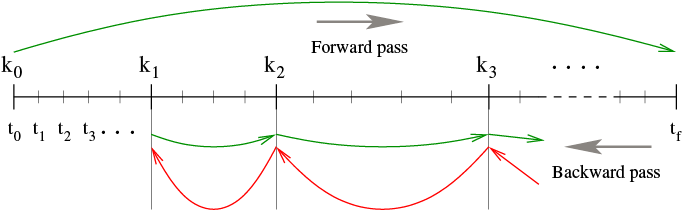
\includegraphics[width=4in]{ckpnt}}
\caption {Illustration of the checkpointing algorithm for generation of
  the forward solution during the integration of the adjoint system.}
\label{f:ckpnt}
\end{figure}

This approach transfers the uncertainty in the number of integration
steps in the forward integration phase to uncertainty in the final
number of checkpoints.  However, $N_c$ is much smaller than the number
of steps taken during the forward integration, and there is no major
penalty for writing/reading the checkpoint data to/from a temporary
file.
%
Note that, at the end of the first forward integration stage, interpolation
data are available from the last checkpoint to the end of the interval
of integration.  If no checkpoints are necessary ($N_d$ is larger than the
number of integration steps taken in the solution of (\ref{e:DAE_p})),
the total cost of an adjoint sensitivity computation can be as low as one forward
plus one backward integration.
%
In addition, {\idas} provides the capability of reusing a set of checkpoints
for multiple backward integrations, thus allowing for efficient computation of
gradients of several functionals (\ref{e:G}).

\bigskip

\index{adjoint sensitivity analysis!implementation in {\idas}|(}
Finally, we note that the adjoint sensitivity module in {\idas} provides the
necessary infrastructure to integrate backwards in time any DAE terminal value
problem dependent on the solution of the IVP (\ref{e:DAE_p}), including
adjoint systems (\ref{e:adj_eqns}) or (\ref{e:adj1_eqns}), as well as any other
quadrature ODEs that may be needed in evaluating the integrals in (\ref{e:dGdp}).
In particular, for DAE systems arising from semi-discretization
of time-dependent PDEs, this feature allows for integration of either the
discretized adjoint PDE system or the adjoint of the discretized PDE.
\index{adjoint sensitivity analysis!implementation in {\idas}|)}
\index{adjoint sensitivity analysis!mathematical background|)}

%----------------------------------------
\section{Second-order sensitivity analysis}\label{ss:hess_sensi}
%----------------------------------------
\index{second-order sensitivity analysis}
In some applications (e.g., dynamically-constrained optimization) it may
be desirable to compute second-order derivative information. Considering
the DAE problem (\ref{e:DAE_p}) and some model output
functional\footnote{For the sake of simplifity in presentation, we do not
include explicit dependencies of $g$ on time $t$ or parameters $p$.
Moreover, we only consider the case in which the dependency of the
original DAE (\ref{e:DAE_p}) on the parameters $p$ is through its initial conditions only.
For details on the derivation in the general case, see~\cite{OzBa:05}.}
$g(y)$, the Hessian $d^2g/dp^2$ can be obtained in a forward sensitivity
analysis setting as
\begin{equation*}
\frac{d^2 g}{d p^2} = \left(g_y \otimes I_{N_p} \right ) y_{pp} + y_p^T g_{yy} y_p \, ,
\end{equation*}
where $\otimes$ is the Kronecker product. The second-order sensitivities are
solution of the matrix DAE system:
\begin{equation*}
  \begin{split}
  & \left( F_{\dot y} \otimes I_{N_p} \right) \cdot \dot y_{pp}  +
  \left( F_y        \otimes I_{N_p} \right) \cdot y_{pp}       +
  \left( I_N \otimes {\dot y}_p^T \right) \cdot \left( F_{\dot y \dot y} \dot y_p + F_{y \dot y} y_p \right) +
  \left( I_N \otimes y_p^T        \right) \cdot \left( F_{y \dot y}      \dot y_p + F_{y y}      y_p \right) = 0 \\
  & y_{pp}(t_0) = \frac{\partial^2 y_0}{\partial p^2} \, , \quad
  \dot y_{pp}(t_0) = \frac{\partial^2 \dot y_0}{\partial p^2} \, ,
  \end{split}
\end{equation*}
where $y_p$ denotes the first-order sensitivity matrix, the solution of $N_p$
systems (\ref{e:sens_eqns}), and $y_{pp}$ is a third-order tensor.
%%
It is easy to see that, except for situations in which the number of parameters
$N_p$ is very small, the computational cost of this so-called {\em forward-over-forward}
approach is exorbitant as it requires the solution of $N_p + N_p^2$ additional
DAE systems of the same dimension as (\ref{e:DAE_p}).

A much more efficient alternative is to compute Hessian-vector products using
a so-called {\em forward-over-adjoint} approach. This method is based on using
the same ``trick'' as the one used in computing gradients of pointwise
functionals with the adjoint method, namely applying a formal directional forward
derivation to the gradient of (\ref{e:dGdp}) (or the equivalent one for a pointwise
functional $g(T, y(T))$). With that, the cost of computing a full Hessian is roughly
equivalent to the cost of computing the  gradient with forward sensitivity analysis.
However, Hessian-vector products can be cheaply computed with one additional adjoint solve.

As an illustration\footnote{The derivation for the general DAE case is too
involved for the purposes of this discussion.}, consider the ODE problem
\begin{equation*}
{\dot y}  = f(t,\,y) \, , \quad y(t_0)  = y_0(p) \, ,
\end{equation*}
depending on some parameters $p$ through the initial conditions only and
consider the model functional output $G(p) = \int_{t_0}^{t_f} g(t,y) \, dt$.
It can be shown that the product between the Hessian of $G$ (with respect to the
parameters $p$) and some vector $u$ can be computed as
\begin{equation*}
  \frac{\partial^2 G}{\partial p^2} u =
  \left[ \left(\lambda^T \otimes I_{N_p} \right) y_{pp}u + y_p^T \mu \right]_{t=t_0} \, ,
\end{equation*}
where $\lambda$ and $\mu$ are solutions of
\begin{equation}
  \begin{split}
    &-\dot\mu = f_y^T\mu + \left(\lambda^T \otimes I_n \right) f_{yy} s \, ; \quad \mu(t_f) = 0 \\
    &-\dot\lambda = f_y^T\lambda + g_y^T \, ; \quad \lambda(t_f) = 0 \\
    &\dot s = f_y s \, ; \quad s(t_0) = y_{0p} u .
  \end{split}
\end{equation}
In the above equation, $s = y_p u$ is a linear combination of the columns of the
sensitivity matrix $y_p$. The {\em forward-over-adjoint}
approach hinges crucially on the fact that $s$ can be computed at the cost of
a forward sensitivity analysis with respect to a single parameter (the last
ODE problem above) which is possible due to the linearity of the forward
sensitivity equations (\ref{e:sens_eqns}).

Therefore (and this is also valid for the DAE case), the cost of computing the
Hessian-vector product is roughly that of two forward and two backward integrations
of a system of DAEs of size $N$.
For more details, including the corresponding formulas for a pointwise model
functional output, see the work by Ozyurt and Barton~\cite{OzBa:05} who discuss
this problem for ODE initial value problems. As far as we know, there is no
published equivalent work on DAE problems. However, the derivations given
in~\cite{OzBa:05} for ODE problems can be extended to DAEs with some careful
consideration given to the derivation of proper final conditions on the
adjoint systems, following the ideas presented in~\cite{CLPS:03}.

\bigskip

\index{second-order sensitivity analysis!support in {\idas}|(}
To allow the {\em foward-over-adjoint} approach described above, {\idas} provides support for:
\begin{itemize}
\item the integration of multiple backward problems depending on the same
  underlying forward problem (\ref{e:DAE_p}), and
\item the integration of backward problems and computation of backward quadratures
  depending on both the states $y$ and forward sensitivities (for this particular
  application, $s$) of the original problem (\ref{e:DAE_p}).
\end{itemize}
\index{second-order sensitivity analysis!support in {\idas}|)}

\clearemptydoublepage
%===============================================================
% IDA Code Organization
%===================================================================================
\chapter{Code Organization}\label{s:organization}
%===================================================================================

%----------------------------------
\section{SUNDIALS organization}\label{ss:sun_org}
%----------------------------------
% This is a shared SUNDIALS TEX file with description of
% the SUNDIALS organization
%
The family of solvers referred to as {\sundials} consists of the solvers
{\cvode} and {\arkode} (for ODE systems), {\kinsol} (for nonlinear algebraic
systems), and {\ida} (for differential-algebraic systems).  In addition,
{\sundials} also includes variants of {\cvode} and {\ida} with sensitivity analysis
capabilities (using either forward or adjoint methods), called {\cvodes} and
{\idas}, respectively.

The various solvers of this family share many subordinate modules.
For this reason, it is organized as a family, with a directory
structure that exploits that sharing (see Figures \ref{f:sunorg1} and
\ref{f:sunorg2}).
%%
%%
\begin{figure}[htb]
{\centerline{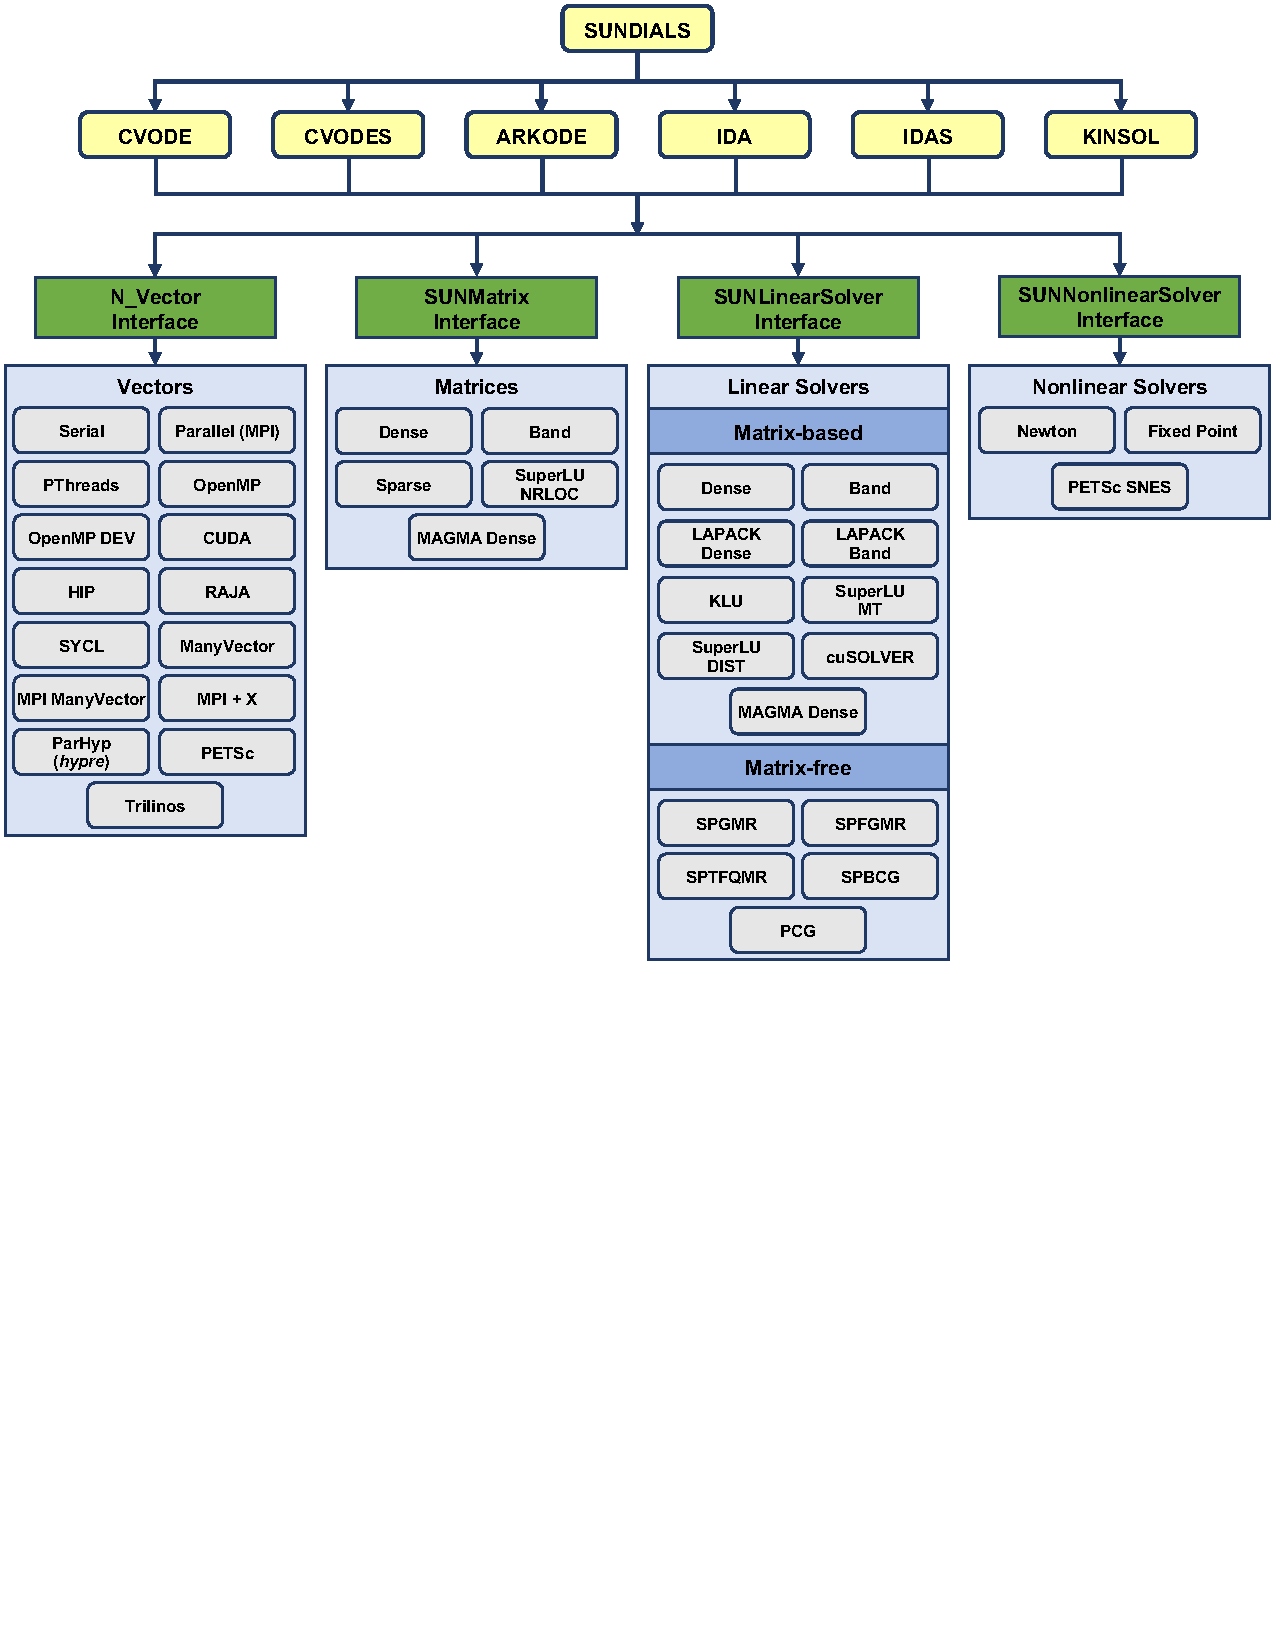
\includegraphics[width=\textwidth]{sunorg1}}}
\caption {High-level diagram of the {\sundials} suite.}\label{f:sunorg1}
\end{figure}
%%
%%
\begin{figure}[htb]
{\centerline{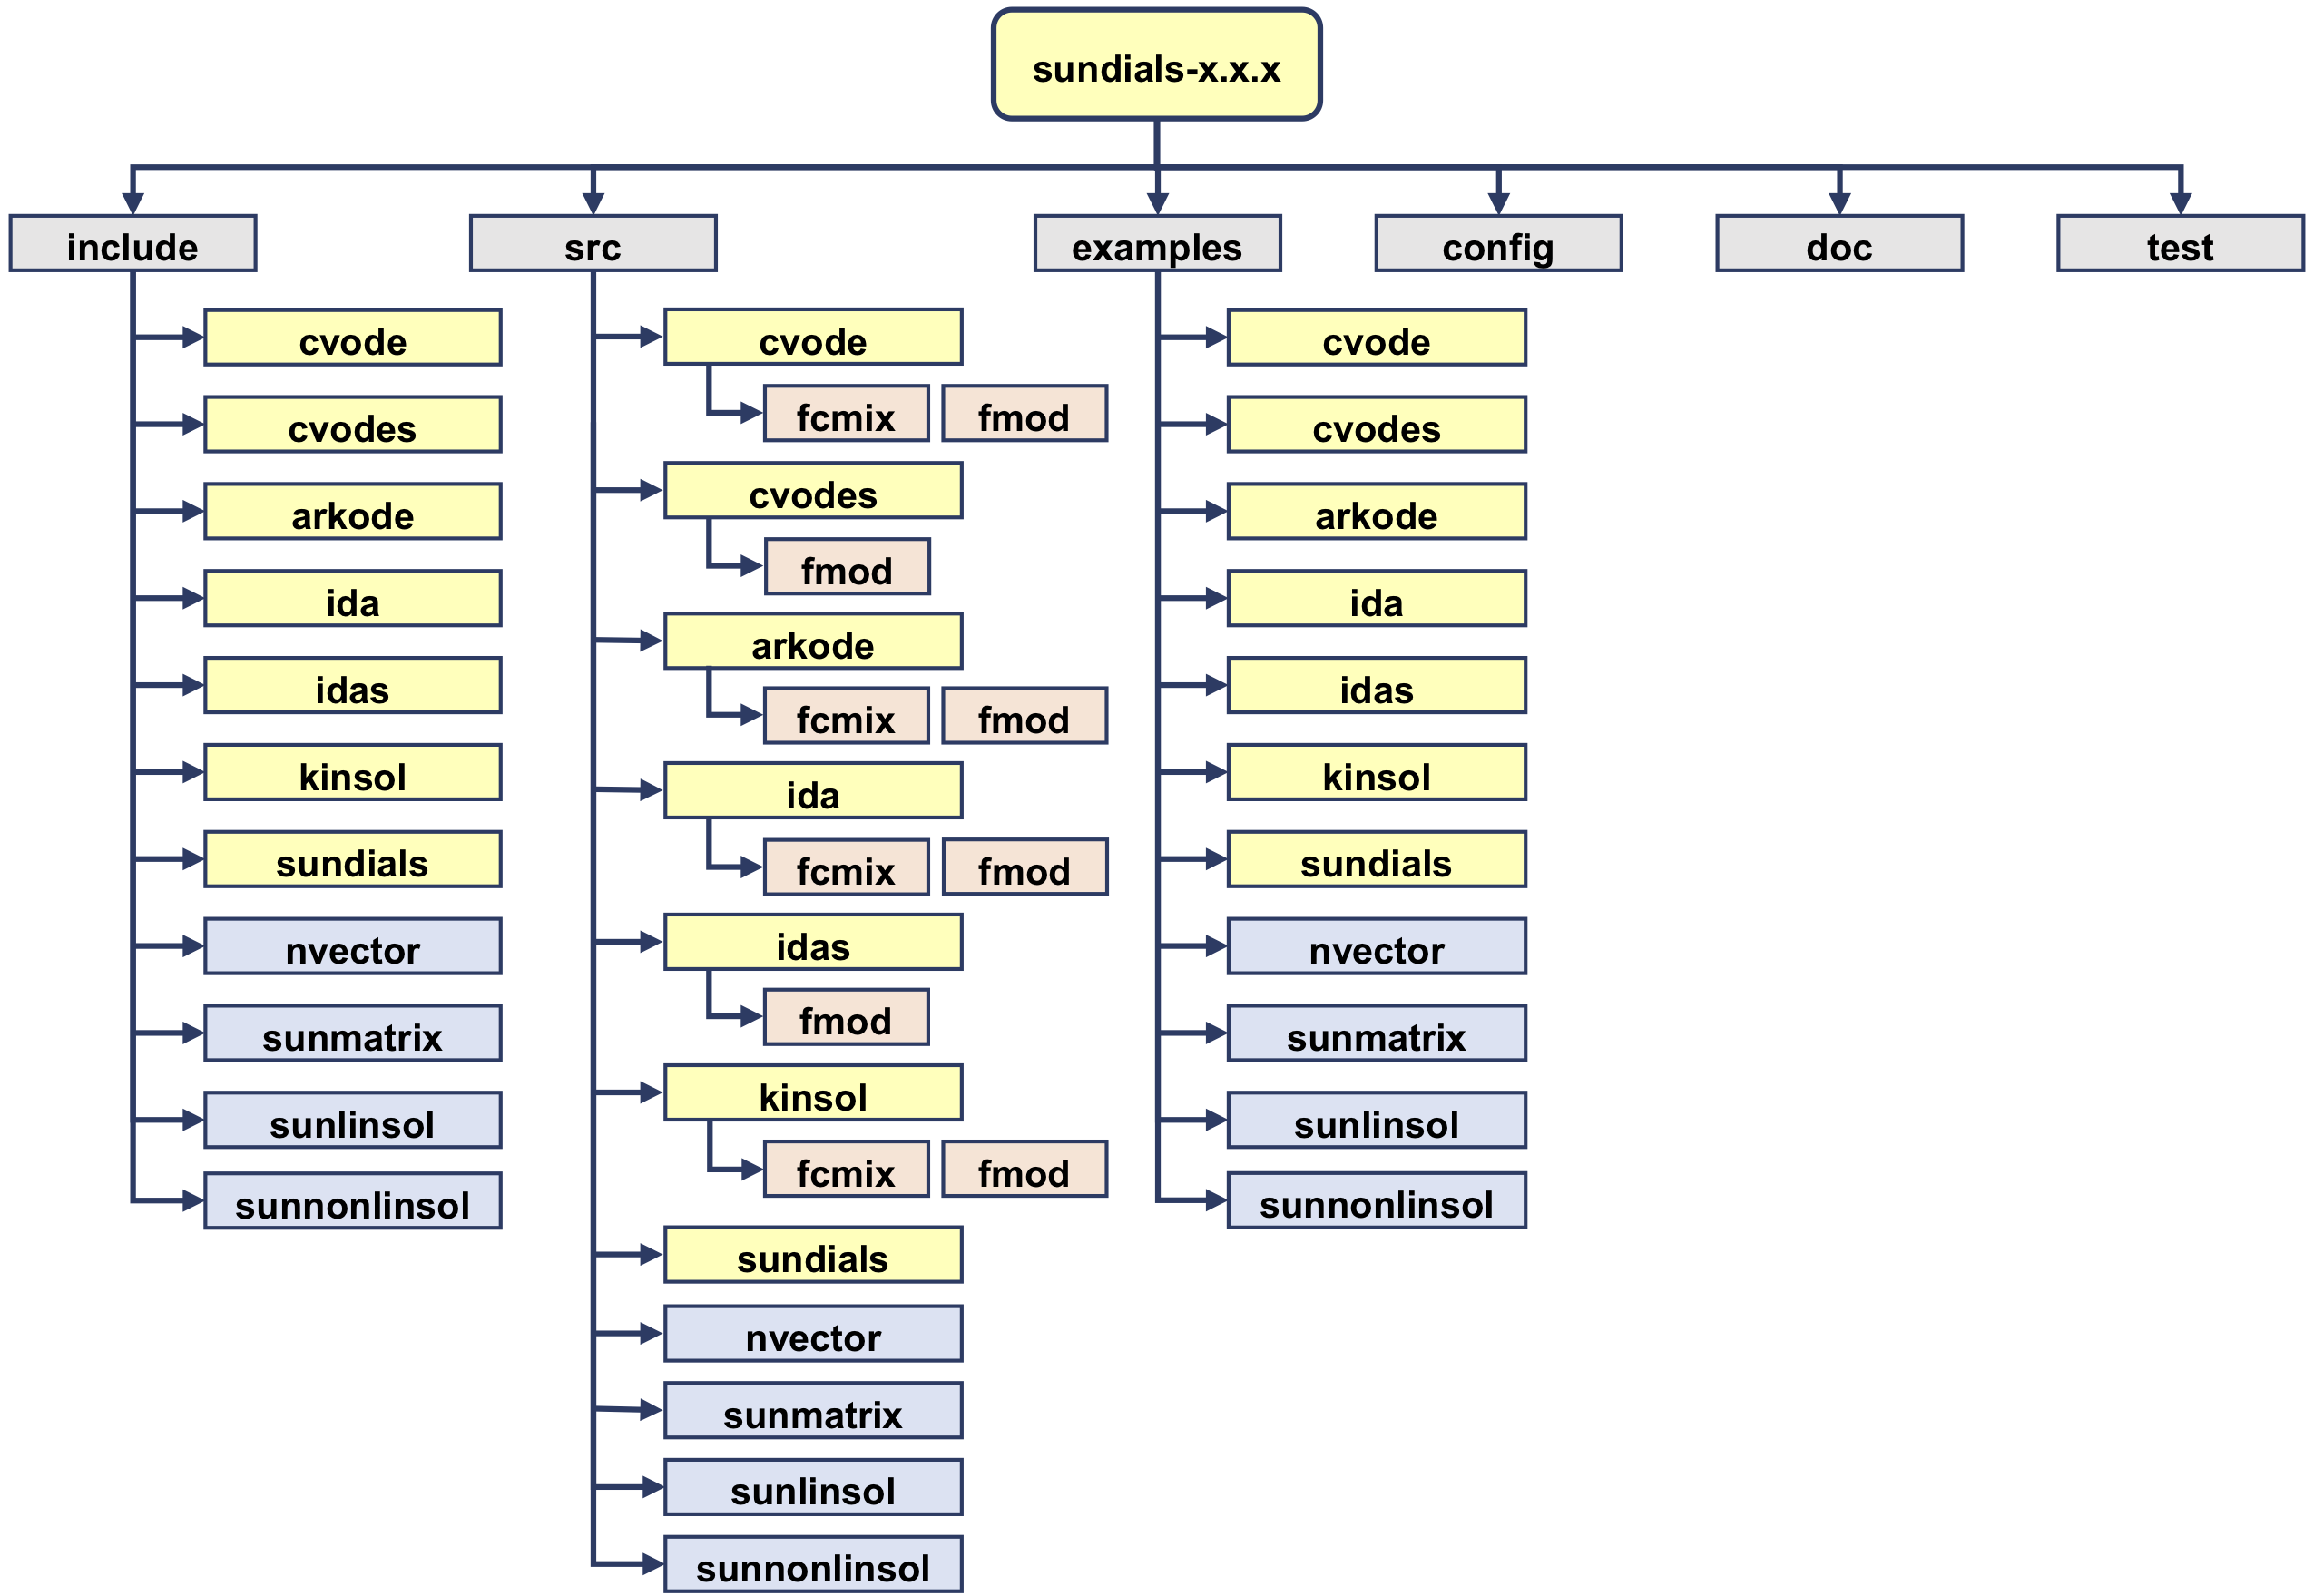
\includegraphics[width=\textwidth]{sunorg2}}}
\caption {Directory structure of the {\sundials} source tree.}\label{f:sunorg2}
\end{figure}
%%
%%
The following is a list of the solver packages presently available, and
the basic functionality of each:
\begin{itemize}

\item {\cvode},
  a solver for stiff and nonstiff ODE systems $dy/dt = f(t,y)$ based
  on Adams and BDF methods;

\item {\cvodes},
  a solver for stiff and nonstiff ODE systems with sensitivity analysis capabilities;

\item {\arkode},
  a solver for stiff, nonstiff, mixed stiff-nonstiff, and multirate ODE systems
  $M dy/dt = f_1(t,y) + f_2(t,y)$ based on Runge-Kutta methods;

\item {\ida},
  a solver for differential-algebraic systems $F(t,y,\dot{y}) = 0$ based on BDF methods;

\item {\idas},
  a solver for differential-algebraic systems
  with sensitivity analysis capabilities;

\item {\kinsol},
  a solver for nonlinear algebraic systems $F(u) = 0$.

\end{itemize}
Note for modules that provide interfaces to third-party libraries (i.e., LAPACK,
{\klu}, {\superlumt}, {\superludist}, {\hypre}, {\petsc}, {\trilinos}, and
{\raja}) users will need to download and compile those packages independently.


%----------------------------------
\section{IDAS organization}\label{ss:idas_org}
%----------------------------------

\index{IDAS@{\idas}!package structure}
The {\idas} package is written in the ANSI {\CC} language. The following
summarizes the basic structure of the package, although knowledge
of this structure is not necessary for its use.

The overall organization of the {\idas} package is shown in Figure
\ref{f:idasorg}.
\begin{figure}[!htb]
{\centerline{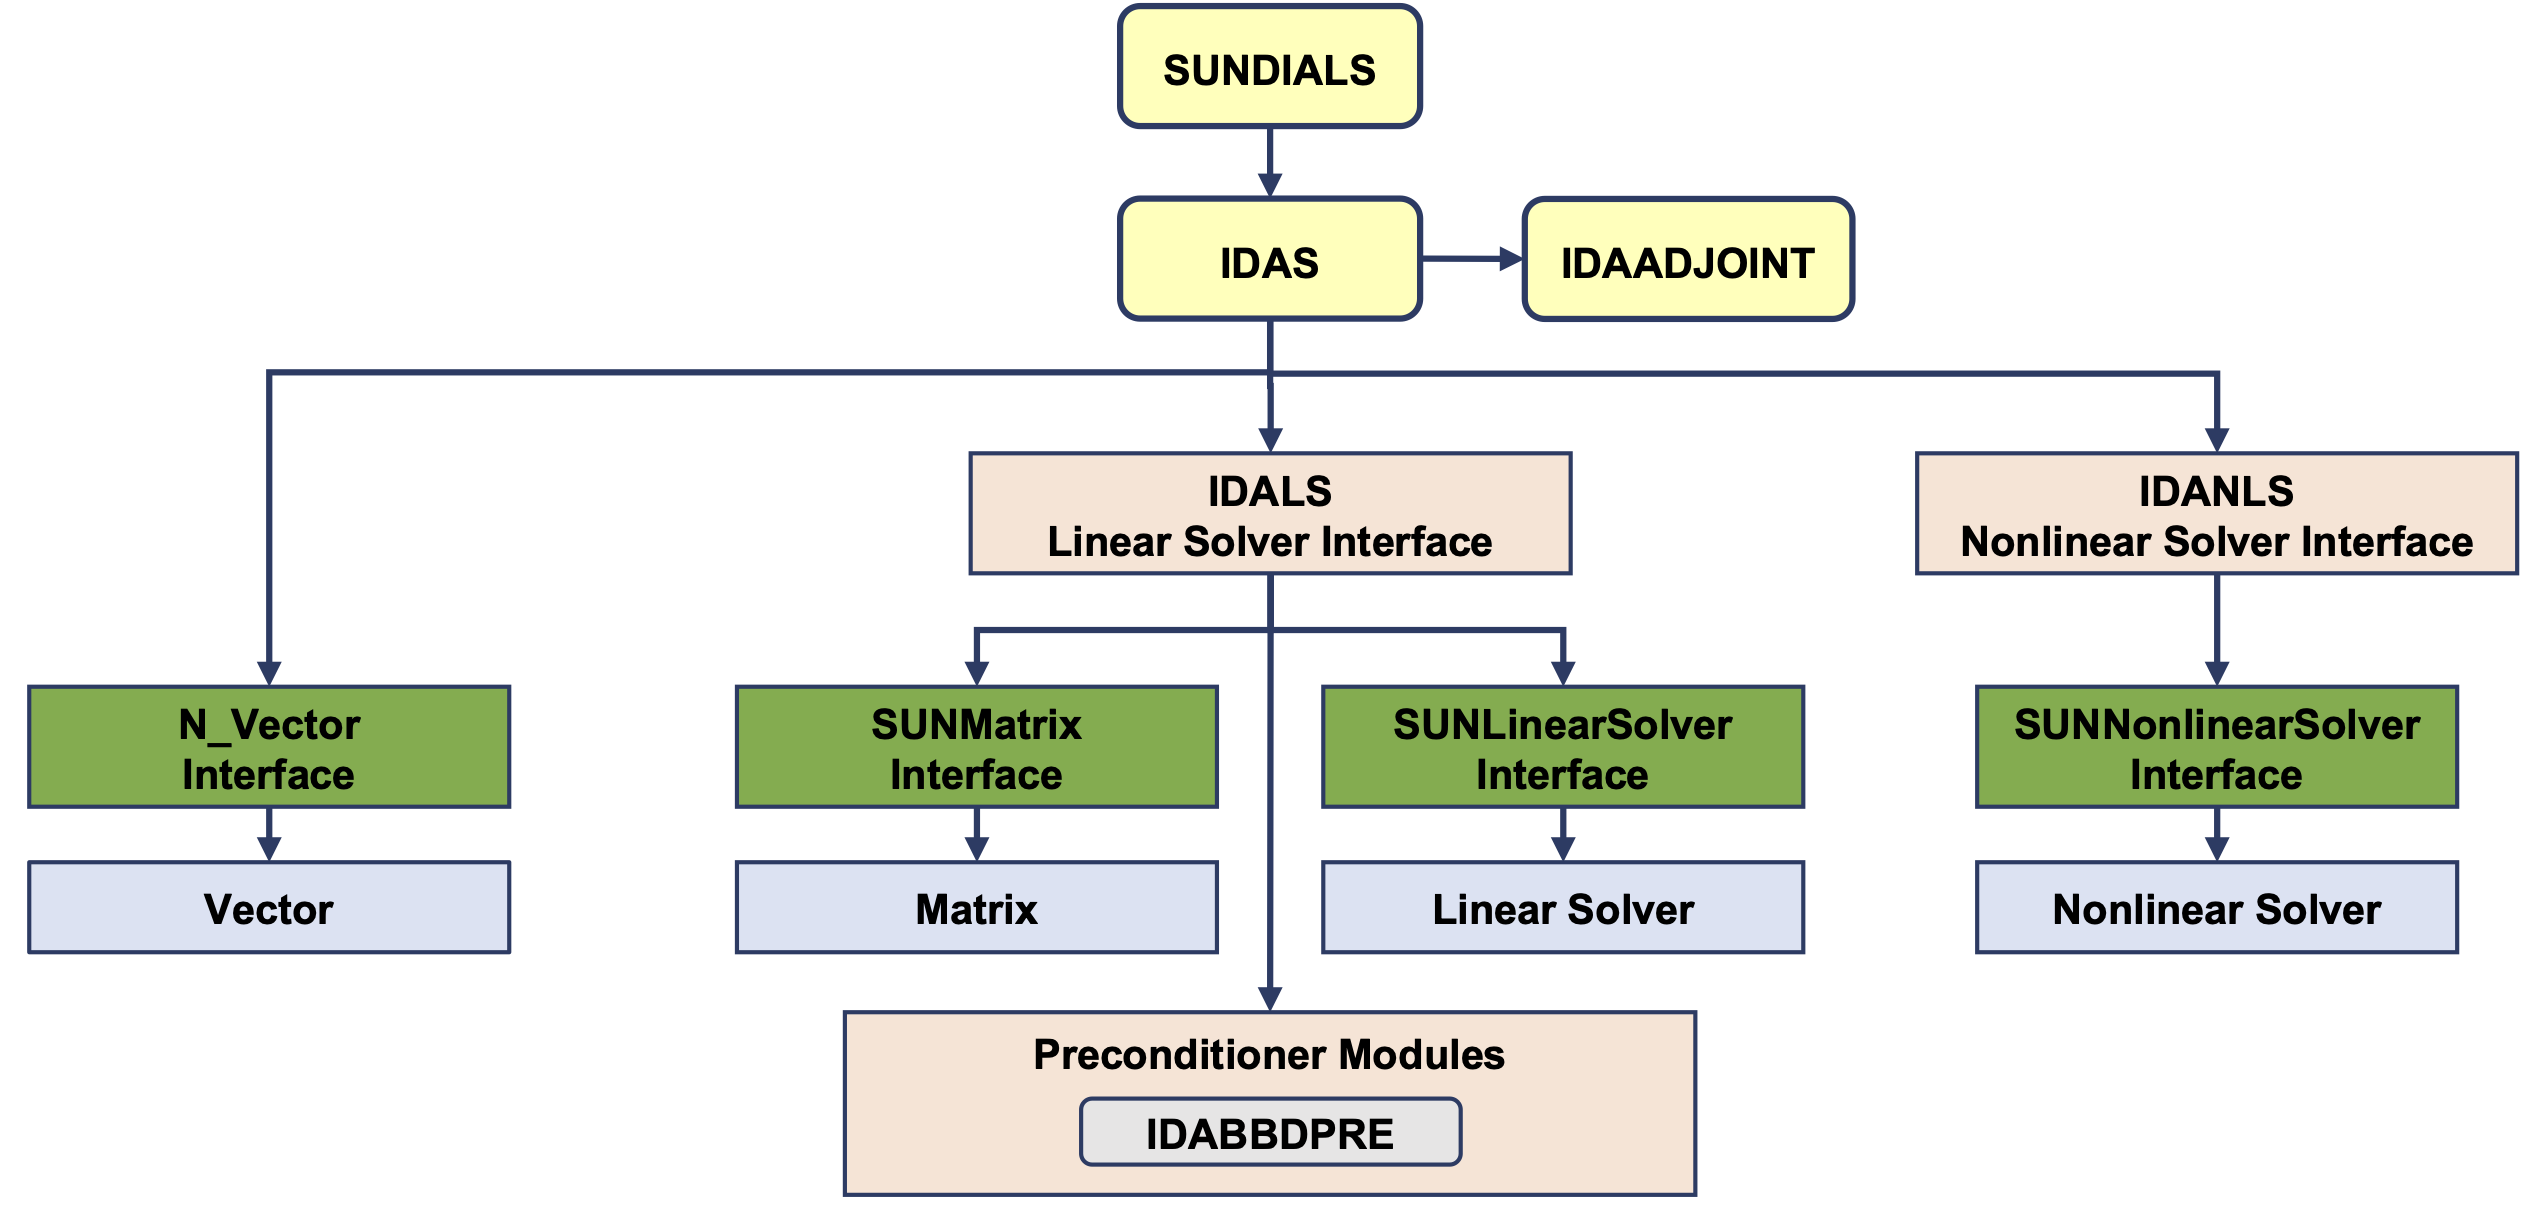
\includegraphics[width=\textwidth]{idasorg}}}
\caption [Overall structure diagram of the {\idas} package]
{Overall structure diagram of the {\idas} package.
  Modules specific to {\idas} begin with ``IDA'' ({\idals}, {\idanls}, and
  {\idabbdpre}), all other items correspond to generic
  {\sundials} vector, matrix, and solver modules (see Figure \ref{f:sunorg1}).}
\label{f:idasorg}
\end{figure}
The central integration module, implemented in the files \id{idas.h},
\id{idas\_impl.h}, and \id{idas.c}, deals with the evaluation of integration
coefficients, estimation of local error,
selection of stepsize and order, and interpolation to user output
points, among other issues.

{\idas} utilizes generic linear and nonlinear solver modules defined by the
{\sunlinsol} API (see Chapter \ref{s:sunlinsol}) and {\sunnonlinsol} API (see
Chapter \ref{c:sunnonlinsol}) respectively. As such, {\idas} has no knowledge
of the method being used to solve the linear and nonlinear systems that
arise in each time step. For any given user problem, there exists a single
nonlinear solver interface and, if necessary, one of the linear system solver
interfaces is specified, and invoked as needed during the integration. While
{\sundials} includes a fixed-point nonlinear solver module, it is not currently
supported in {\idas} (note the fixed-point module is listed in Figure
\ref{f:sunorg1} but not Figure \ref{f:idasorg}).

In addition, if forward sensitivity analysis is turned on, the main module
will integrate the forward sensitivity equations simultaneously with the original
IVP. The sensitivity variables may be included in the local error control
mechanism of the main integrator.
\index{forward sensitivity analysis!correction strategies}
{\idas} provides two different strategies for dealing with the correction
stage for the sensitivity variables: \Id{IDA\_SIMULTANEOUS} \Id{IDA\_STAGGERED}
(see \S\ref{ss:fwd_sensi}).
The {\idas} package includes an algorithm for the approximation of the
sensitivity equations residuals by difference quotients, but the user has
the option of supplying these residual functions directly.

\index{adjoint sensitivity analysis!implementation in {\idas}|(}
The adjoint sensitivity module (file \id{idaa.c}) provides the infrastructure needed for the
backward integration of any system of DAEs which depends on the solution
of the original IVP, in particular the adjoint system and any quadratures required
in evaluating the gradient of the objective functional.  This module deals with
the setup of the checkpoints, the interpolation of the forward solution during
the backward integration, and the backward integration of the adjoint equations.
\index{adjoint sensitivity analysis!implementation in {\idas}|)}

\index{IDAS@{\ida} linear solver interfaces|(}
{\idas} now has a single unified linear solver interface, {\idals},
supporting both direct and iterative linear solvers built using the
generic {\sunlinsol} API (see Chapter \ref{s:sunlinsol}).  These
solvers may utilize a {\sunmatrix} object (see Chapter
\ref{s:sunmatrix}) for storing Jacobian information, or they may be
matrix-free.  Since {\idas} can operate on any valid {\sunlinsol}
implementation, the set of linear solver modules available to {\idas}
will expand as new {\sunlinsol} modules are developed.

For users employing dense or banded Jacobian matrices, {\idals}
includes algorithms for their approximation through difference
quotients, but the user also has the option of supplying the Jacobian
(or an approximation to it) directly.  This user-supplied
routine is required when using sparse or user-supplied Jacobian
matrices.

For users employing matrix-free iterative linear solvers, {\idals}
includes an algorithm for the approximation by difference quotients of
the product between the Jacobian matrix and a vector, $Jv$. Again, the
user has the option of providing routines for this operation, in two
phases: setup (preprocessing of Jacobian data) and multiplication.

For preconditioned iterative methods, \index{preconditioning!setup and solve phases}
the preconditioning must be supplied by the user, again in two phases:
setup and solve.  While\index{preconditioning!advice on} there is no
default choice of preconditioner analogous to the difference-quotient
approximation in the direct case, the references
\cite{BrHi:89,Byr:92}, together with the example and demonstration
programs included with {\idas}, offer considerable assistance in
building preconditioners.

\index{IDAS@{\idas} linear solvers!implementation details|(}
{\idas}' linear solver interface consists of four primary routines,
devoted to (1) memory allocation and initialization, (2) setup of the
matrix data involved, (3) solution of the system, and (4) freeing of memory.
The setup and solution phases are separate because the evaluation of
Jacobians and preconditioners is done only periodically during the
integration, as required to achieve convergence. The call list within
the central {\idas} module to each of the four associated functions is
fixed, thus allowing the central module to be completely independent
of the linear system method.
\index{IDAS@{\idas} linear solvers!implementation details|)}

{\idas} also provides a preconditioner module, {\idabbdpre}, for use
with any of the Krylov iterative linear solvers.  It works in
conjunction with {\nvecp} and generates a preconditioner that is a
block-diagonal matrix with each block being a banded matrix.

All state information used by {\idas} to solve a given problem is saved
in a structure, and a pointer to that structure is returned to the
user.  There is no global data in the {\idas} package, and so, in this
respect, it is reentrant. State information specific to the linear
solver is saved in a separate structure, a pointer to which resides in
the {\idas} memory structure. The reentrancy of {\idas} was motivated
by the situation where two or more problems are solved by
intermixed calls to the package from one user program.

\clearemptydoublepage
%===============================================================
% Usage for simulation
%%==================================================================================
\chapter{Using IDAS for IVP Solution}\label{s:simulation}
%%===================================================================================

This chapter is concerned with the use of {\idas} for the integration
of DAEs in a C language setting.  The following sections treat the header files,
the layout of the user's main program, description of the {\idas} user-callable
functions, and description of user-supplied functions.
This usage is essentially equivalent to using {\ida}~\cite{ida_ug}.

The sample programs described in the companion document \cite{idas_ex}
may also be helpful. Those codes may be used as templates (with the removal of
some lines involved in testing), and are included in the {\idas} package.

The user should be aware that not all {\sunlinsol} and {\sunmatrix}
modules are compatible with all {\nvector} implementations.
\index{IDAS@{\idas} linear solvers!NVECTOR@{\nvector} compatibility}
Details on compatibility are given in the documentation for each
{\sunmatrix} module (Chapter \ref{s:sunmatrix}) and each {\sunlinsol}
module (Chapter \ref{s:sunlinsol}). For example, {\nvecp} is not
compatible with the dense, banded, or sparse {\sunmatrix} types, or with
the corresponding dense, banded, or sparse {\sunlinsol} modules.  Please
check Chapters \ref{s:sunmatrix} and \ref{s:sunlinsol} to verify
compatibility between these modules.  In addition to that
documentation, we note that the preconditioner module {\idabbdpre}
can only be used with {\nvecp}.
It is not recommended to use a threaded vector module with SuperLU\_MT
unless it is the {\nvecopenmp} module, and SuperLU\_MT is also compiled
with OpenMP.

{\idas} uses various constants for both input and output.  These are
defined as needed in this chapter, but for convenience are also listed
separately in Appendix \ref{c:constants}.

%%==============================================================================
\section{Access to library and header files}\label{ss:file_access}
%%==============================================================================

At this point, it is assumed that the installation of {\idas},
following the procedure described in Appendix \ref{c:install}, has
been completed successfully.

Regardless of where the user's application program resides, its
associated compilation and load commands must make reference to the
appropriate locations for the library and header files required by
{\idas}.  The relevant library files are
\begin{itemize}
\item {\em libdir}\id{/libsundials\_idas.}{\em lib},
\item {\em libdir}\id{/libsundials\_nvec*.}{\em lib},
\end{itemize}
where the file extension .{\em lib} is typically \id{.so} for shared libraries
and \id{.a} for static libraries. The relevant header files are located in
the subdirectories
\begin{itemize}
\item {\em incdir}\id{/include/idas}
\item {\em incdir}\id{/include/sundials}
\item {\em incdir}\id{/include/nvector}
\item {\em incdir}\id{/include/sunmatrix}
\item {\em incdir}\id{/include/sunlinsol}
\item {\em incdir}\id{/include/sunnonlinsol}
\end{itemize}
The directories {\em libdir} and {\em incdir} are the install library
and include directories, respectively. For a default installation,
these are {\em instdir}\id{/lib} and {\em instdir}\id{/include},
respectively, where {\em instdir} is the directory where {\sundials}
was installed (see Appendix \ref{c:install}).

Note that an application cannot link to both the {\ida} and {\idas} libraries
because both contain user-callable functions with the same names (to ensure that {\idas}
is backward compatible with {\ida}). Therefore, applications that contain both
DAE problems and DAEs with sensitivity analysis, should use {\idas}.

%%===================================================================================
\section{Data types}\label{s:types}
%%===================================================================================
% This is a shared SUNDIALS TEX file with description of
% types used in llntyps.h
%
\index{portability}
The \ID{sundials\_types.h} file contains the definition of the type \ID{realtype},
which is used by the {\sundials} solvers for all floating-point data, the definition
of the integer type \ID{sunindextype}, which is used for vector and matrix indices,
and \ID{booleantype}, which is used for certain logic operations within {\sundials}.


\subsection{Floating point types}

The type \id{realtype} can be \id{float}, \id{double}, or \id{long double}, with
the default being \id{double}.
The user can change the precision of the {\sundials} solvers arithmetic at the
configuration stage (see \S\ref{ss:configuration_options_nix}).

Additionally, based on the current precision, \id{sundials\_types.h} defines
\Id{BIG\_REAL} to be the largest value representable as a \id{realtype},
\Id{SMALL\_REAL} to be the smallest value representable as a \id{realtype}, and
\Id{UNIT\_ROUNDOFF} to be the difference between $1.0$ and the minimum \id{realtype}
greater than $1.0$.

Within {\sundials}, real constants are set by way of a macro called
\Id{RCONST}.  It is this macro that needs the ability to branch on the
definition \id{realtype}.  In ANSI {\CC}, a floating-point constant with no
suffix is stored as a \id{double}.  Placing the suffix ``F'' at the
end of a floating point constant makes it a \id{float}, whereas using the suffix
``L'' makes it a \id{long double}.  For example,
\begin{verbatim}
#define A 1.0
#define B 1.0F
#define C 1.0L
\end{verbatim}
defines \id{A} to be a \id{double} constant equal to $1.0$, \id{B} to be a
\id{float} constant equal to $1.0$, and \id{C} to be a \id{long double} constant
equal to $1.0$.  The macro call \id{RCONST(1.0)} automatically expands to \id{1.0}
if \id{realtype} is \id{double}, to \id{1.0F} if \id{realtype} is \id{float},
or to \id{1.0L} if \id{realtype} is \id{long double}.  {\sundials} uses the
\id{RCONST} macro internally to declare all of its floating-point constants.

Additionally, {\sundials} defines several macros for common mathematical
functions \textit{e.g.}, \id{fabs}, \id{sqrt}, \id{exp}, etc. in
\id{sundials\_math.h}. The macros are prefixed with \id{SUNR} and expand to the
appropriate \id{C} function based on the \id{realtype}. For example, the macro
\id{SUNRabs} expands to the \id{C} function \id{fabs} when \id{realtype} is
\id{double}, \id{fabsf} when \id{realtype} is \id{float}, and \id{fabsl} when
\id{realtype} is \id{long double}.

A user program which uses the type \id{realtype}, the \id{RCONST} macro, and the
\id{SUNR} mathematical function macros is precision-independent except for any
calls to  precision-specific library functions. Our example programs use
\id{realtype}, \id{RCONST}, and the \id{SUNR} macros. Users can, however, use
the type \id{double}, \id{float}, or \id{long double} in their code (assuming
that this usage is consistent with the typedef for \id{realtype}) and call the
appropriate math library functions directly. Thus, a previously existing piece
of ANSI {\CC} code can use {\sundials} without modifying the code to use
\id{realtype}, \id{RCONST}, or the \id{SUNR} macros so long as the {\sundials}
libraries use the correct precision (for details see
\S\ref{ss:configuration_options_nix}).


\subsection{Integer types used for indexing}

The type \id{sunindextype} is used for indexing array entries in {\sundials}
modules (\textit{e.g.}, vectors lengths and matrix sizes) as well as for storing
the total problem size. During configuration \id{sunindextype} may be selected
to be either a 32- or 64-bit \emph{signed} integer with the default being
64-bit. See \S\ref{ss:configuration_options_nix} for the configuration option
to select the desired size of \id{sunindextype}. When using a 32-bit integer the
total problem size is limited to $2^{31}-1$ and with 64-bit integers the limit
is $2^{63}-1$. For users with problem sizes that exceed the 64-bit limit an
advanced configuration option is available to specify the type used for
\id{sunindextype}.

A user program which uses \id{sunindextype} to handle indices will work with
both index storage types except for any calls to index storage-specific
external libraries. Our \id{C} and \id{C++} example programs
use \id{sunindextype}. Users can, however, use any compatible type
(\textit{e.g.}, \id{int}, \id{long int}, \id{int32\_t}, \id{int64\_t}, or
\id{long long int}) in their code, assuming that this usage is consistent with
the typedef for \id{sunindextype} on their architecture. Thus, a previously
existing piece of ANSI {\CC} code can use {\sundials} without modifying the code
to use \id{sunindextype}, so long as the {\sundials} libraries use the
appropriate index storage type (for details see
\S\ref{ss:configuration_options_nix}).


%%===================================================================================
\section{Header files}\label{ss:header_sim}
%%===================================================================================
\index{header files}
The calling program must include several header files so that various macros
and data types can be used. The header file that is always required is:
%%
\begin{itemize}
\item  \Id{idas/idas.h},
  the header file for {\idas}, which defines the several
  types and various constants, and includes function prototypes.  This
  includes the header file for {\idals}, \Id{ida/ida\_ls.h}.
\end{itemize}
%%
Note that \id{idas.h} includes \Id{sundials\_types.h},
which defines the types \id{realtype}, \id{sunindextype}, and \id{booleantype}
and the constants \id{SUNFALSE} and \id{SUNTRUE}.

The calling program must also include an {\nvector} implementation header file,
of the form \\ \noindent
\id{nvector/nvector\_***.h}.  See Chapter \ref{s:nvector} for the appropriate
name.  This file in turn includes the header file \Id{sundials\_nvector.h}
which defines the abstract \Id{N\_Vector} data type.

If using a non-default nonlinear solver module, or when interacting
with a {\sunnonlinsol} module directly, the calling program must also
include a {\sunnonlinsol} implementation header file, of the form
\id{sunnonlinsol/sunnonlinsol\_***.h} where \id{***} is the name of the
nonlinear solver module (see Chapter \ref{c:sunnonlinsol} for more
information). This file in turn includes the header file
\Id{sundials\_nonlinearsolver.h} which defines the abstract
\Id{SUNNonlinearSolver} data type.

If using a nonlinear solver that requires the solution of a linear
system of the form (\ref{e:DAE_Newtoncorr}) (e.g., the default Newton
iteration), a linear solver module header file is also required.
\index{IDAS@{\idas} linear solvers!header files}
The header files corresponding to the various {\sundials}-provided
linear solver modules available for use with {\idas} are:
%%
\begin{itemize}
\item Direct linear solvers:
  \begin{itemize}
  \item \Id{sunlinsol/sunlinsol\_dense.h},
    which is used with the dense linear solver module,
    {\sunlinsoldense};

  \item \Id{sunlinsol/sunlinsol\_band.h},
    which is used with the banded linear solver module,
    {\sunlinsolband};

  \item \Id{sunlinsol/sunlinsol\_lapackdense.h},
    which is used with the LAPACK dense linear solver module,
    {\sunlinsollapdense};

  \item \Id{sunlinsol/sunlinsol\_lapackband.h},
    which is used with the LAPACK banded linear solver module,
    {\sunlinsollapband};

  \item \Id{sunlinsol/sunlinsol\_klu.h},
    which is used with the {\klu} sparse linear solver module,
    {\sunlinsolklu};

  \item \Id{sunlinsol/sunlinsol\_superlumt.h},
    which is used with the {\superlumt} sparse linear solver
    module, {\sunlinsolslumt};
  \end{itemize}

\item Iterative linear solvers:
  \begin{itemize}
  \item \Id{sunlinsol/sunlinsol\_spgmr.h},
    which is used with the scaled, preconditioned GMRES Krylov linear
    solver module, {\sunlinsolspgmr};

  \item \Id{sunlinsol/sunlinsol\_spfgmr.h},
    which is used with the scaled, preconditioned FGMRES Krylov linear
    solver module, {\sunlinsolspfgmr};

  \item \Id{sunlinsol/sunlinsol\_spbcgs.h},
    which is used with the scaled, preconditioned Bi-CGStab Krylov
    linear solver module, {\sunlinsolspbcgs};

  \item \Id{sunlinsol/sunlinsol\_sptfqmr.h},
    which is used with the scaled, preconditioned TFQMR Krylov linear
    solver module, {\sunlinsolsptfqmr};

  \item \Id{sunlinsol/sunlinsol\_pcg.h},
    which is used with the scaled, preconditioned CG Krylov linear
    solver module, {\sunlinsolpcg};
  \end{itemize}
\end{itemize}

The header files for the {\sunlinsoldense} and {\sunlinsollapdense}
linear solver modules include the file
\id{sunmatrix/sunmatrix\_dense.h}, which defines the {\sunmatdense}
matrix module, as as well as various functions and macros acting on
such matrices.

The header files for the {\sunlinsolband} and {\sunlinsollapband}
linear solver modules include the file
\id{sunmatrix/sunmatrix\_band.h}, which defines the {\sunmatband}
matrix module, as as well as various functions and macros acting on
such matrices.

The header files for the {\sunlinsolklu} and {\sunlinsolslumt}
sparse linear solvers include the file
\id{sunmatrix/sunmatrix\_sparse.h}, which defines the {\sunmatsparse}
matrix module, as well as various functions and macros acting on such
matrices.

The header files for the Krylov iterative solvers include the file
\id{sundials/sundials\_iterative.h}, which enumerates the kind of
preconditioning, and (for the {\spgmr} and {\spfgmr} solvers) the
choices for the Gram-Schmidt process.

Other headers may be needed, according to the choice of
preconditioner, etc.  For example, in the \id{idasFoodWeb\_kry\_p}
example (see \cite{idas_ex}), preconditioning is done with a
block-diagonal matrix. For this, even though the {\sunlinsolspgmr}
linear solver is used, the header \id{sundials/sundials\_dense.h} is
included for access to the underlying generic dense matrix arithmetic
routines.

%%====================================================================
\section{A skeleton of the user's main program}\label{ss:skeleton_sim}
%%====================================================================
The following is a skeleton of the user's main program (or calling program)
for the integration of a DAE IVP. Most of the steps are independent of the
{\nvector}, {\sunmatrix}, {\sunlinsol}, and {\sunnonlinsol} implementations
used. For the steps that are not, refer to Chapter \ref{s:nvector},
\ref{s:sunmatrix}, \ref{s:sunlinsol}, and \ref{c:sunnonlinsol} for the specific
name of the function to be called or macro to be referenced.
%%
\index{User main program!IDAS@{\idas} usage}
\begin{Steps}

\item
  {\bf Initialize parallel or multi-threaded environment, if appropriate}

  For example, call \id{MPI\_Init} to initialize {\mpi} if used, or
  set \id{num\_threads}, the number of threads to use within the threaded
  vector functions, if used.

\item
  {\bf Set problem dimensions etc.}

  This generally includes the problem size \id{N}, and may include
  the local vector length \id{Nlocal}.

  Note: The variables \id{N} and \id{Nlocal} should be of type \id{sunindextype}.

\item
  {\bf Set vectors of initial values}

  To set the vectors \id{y0} and \id{yp0} to initial values for $y$\ and
  $\dot{y}$, use the appropriate functions defined by the particular
  {\nvector} implementation.

  For native {\sundials} vector implementations
  (except the {\cuda} and {\raja}-based ones),
  use a call of the form \id{y0 = N\_VMake\_***(..., ydata)} if the \id{realtype}
  array \id{ydata} containing the initial values of $y$ already exists.
  Otherwise, create a new vector by making a call of the form
  \id{y0 = N\_VNew\_***(...)}, and then set its elements by accessing
  the underlying data with a call of the form
  \id{ ydata = N\_VGetArrayPointer(y0)}.
  See \S\ref{ss:nvec_ser}-\ref{ss:nvec_pthreads} for details.

  For the {\hypre} and {\petsc} vector wrappers, first create and initialize
  the underlying vector and then create an {\nvector} wrapper with a call
  of the form \id{y0 = N\_VMake\_***(yvec)}, where \id{yvec} is a {\hypre}
  or {\petsc} vector. Note that calls like \id{N\_VNew\_***(...)} and
  \id{N\_VGetArrayPointer(...)} are not available for these vector wrappers.
  See \S\ref{ss:nvec_parhyp} and \S\ref{ss:nvec_petsc} for details.

  If using either the {\cuda}- or {\raja}-based vector implementations
  use a call of the form
  \id{y0 = N\_VMake\_***(..., c)} where \id{c} is a pointer to a \id{suncudavec}
  or \id{sunrajavec} vector class if this class already exists.  Otherwise,
  create a new vector
  by making a call of the form \id{y0 = N\_VNew\_***(...)}, and then set its
  elements by accessing the underlying data where it is located
  with a call of the form
  \id{N\_VGetDeviceArrayPointer\_***} or \id{N\_VGetHostArrayPointer\_***}.
  Note that the vector class will allocate memory on both the host and device
  when instantiated.  See \S\ref{ss:nvec_cuda}-\ref{ss:nvec_raja} for details.

%   If a \id{realtype} array \id{ydata} containing the initial values of $y$
%   already exists, it may be possible to set \id{y0} either with a call of the form
%   \id{y0 = N\_VMake\_***(..., ydata);}
%   or by making a call of the form
%   \id{y0 = N\_VNew\_***(...);}
%   and loading values into the structure defined by \id{NV\_DATA\_***(y0)},
%   provided these functions and macro exist for the {\nvector} module chosen.

  Set the vector \id{yp0} of initial conditions for $\dot{y}$ similarly.

\item\label{i:ida_create}
  {\bf Create {\idas} object}

  Call \id{ida\_mem = }\id{IDACreate}\id{()}
  to create the {\idas} memory block.
  \id{IDACreate} returns a pointer to the {\idas} memory structure.
  See \S\ref{sss:idainit} for details.
  This \id{void *} pointer must then be passed as the first argument
  to all subsequent {\idas} function calls.

\item\label{i:ida_init}
  {\bf Initialize {\idas} solver}

  Call \id{IDAInit}\id{(...)} to provide required problem
  specifications (residual function, initial time, and initial conditions),
  allocate internal memory for {\idas}, and initialize {\idas}.
  \id{IDAInit} returns an error flag to indicate success or an illegal argument
  value.  See \S\ref{sss:idainit} for details.

\item
  {\bf Specify integration tolerances}

  Call \id{IDASStolerances}\id{(...)} or \id{IDASVtolerances}\id{(...)}
  to specify, respectively, a scalar relative tolerance and scalar
  absolute tolerance, or a scalar relative tolerance and a vector of
  absolute tolerances.  Alternatively, call \id{IDAWFtolerances} to
  specify a function which sets directly the weights used in
  evaluating WRMS vector norms.  See \S\ref{sss:idatolerances} for
  details.

\item\label{i:matrix}
  {\bf Create matrix object}

  If a nonlinear solver requiring a linear solver will be used (e.g., the
  default Newton iteration) and the linear solver will be a matrix-based linear
  solver, then a template Jacobian matrix must be created by using the
  appropriate constructor function defined by the particular {\sunmatrix}
  implementation.

  For the {\sundials}-supplied {\sunmatrix} implementations, the
  matrix object may be created using a call of the form

  \id{SUNMatrix J = }\Id{SUNBandMatrix}\id{(...);}

   or

  \id{SUNMatrix J = }\Id{SUNDenseMatrix}\id{(...);}

   or

  \id{SUNMatrix J = }\Id{SUNSparseMatrix}\id{(...);}

  NOTE: The dense, banded, and sparse matrix objects are usable only in a
  serial or threaded environment.

\item\label{i:lin_solver}
  {\bf Create linear solver object}

  If a nonlinear solver requiring a linear solver is chosen (e.g., the default
  Newton iteration), then the desired linear solver object must be created by
  calling the appropriate constructor function defined by the particular
  {\sunlinsol} implementation.

  For any of the {\sundials}-supplied {\sunlinsol} implementations,
  the linear solver object may be created using a call of the form

  \id{SUNLinearSolver LS = SUNLinSol\_*(...);}

  where \id{*} can be replaced with ``Dense'', ``SPGMR'', or other
  options, as discussed in \S\ref{sss:lin_solv_init} and Chapter {\ref{s:sunlinsol}}.

\item
  {\bf Set linear solver optional inputs}

  Call \id{*Set*} functions from the selected linear solver module
  to change optional inputs specific to that linear solver.
  See the documentation for each {\sunlinsol} module in Chapter
  {\ref{s:sunlinsol}} for details.

\item\label{i:lin_solver_interface}
  {\bf Attach linear solver module}

  If a nonlinear solver requiring a linear solver is chosen (e.g., the default
  Newton iteration), then initialize the {\idals} linear solver
  interface by attaching the linear solver object (and matrix object, if
  applicable) with the following call (for details see
  \S\ref{sss:lin_solv_init}):

  \id{ier = }\Id{IDASetLinearSolver}\id{(...);}

\item
  {\bf Set optional inputs}

  Optionally, call \id{IDASet*} functions to change from their default values any
  optional inputs that control the behavior of {\idas}.
  See \S\ref{sss:optin_main} and \S\ref{ss:optional_input} for details.

\item\label{i:nonlin_solver}
  {\bf Create nonlinear solver object} (\textit{optional})

  If using a non-default nonlinear solver (see \S\ref{sss:nonlin_solv_init}),
  then create the desired nonlinear solver object by calling the appropriate
  constructor function defined by the particular {\sunnonlinsol} implementation
  (e.g., \id{NLS = SUNNonlinSol\_***(...);} where \id{***} is the name of the
  nonlinear solver (see Chapter \ref{c:sunnonlinsol} for details).

\item\label{i:nonlin_solver_interface}
  {\bf Attach nonlinear solver module} (\textit{optional})

  If using a non-default nonlinear solver, then initialize the nonlinear solver
  interface by attaching the nonlinear solver object by calling
  \id{ier = }\Id{IDASetNonlinearSolver}\id{(ida\_mem, NLS);} (see
  \S\ref{sss:nonlin_solv_init} for details).

\item
  {\bf Set nonlinear solver optional inputs} (\textit{optional})

  Call the appropriate set functions for the selected nonlinear solver module to
  change optional inputs specific to that nonlinear solver. These \textit{must}
  be called after \id{IDAInit} if using the default nonlinear solver or after
  attaching a new nonlinear solver to {\idas}, otherwise the optional inputs will
  be overridden by {\idas} defaults. See Chapter \ref{c:sunnonlinsol} for more
  information on optional inputs.

\item
  {\bf Correct initial values}

  Optionally, call \id{IDACalcIC} to correct the initial values
  \id{y0} and \id{yp0} passed to \id{IDAInit}.  See \S\ref{ss:idacalcic}.
  Also see \S\ref{sss:optin_iccalc} for relevant optional input calls.

\item
  {\bf Specify rootfinding problem}
  \index{Rootfinding}

  Optionally, call \id{IDARootInit} to initialize a rootfinding problem
  to be solved during the integration of the DAE system.
  See \S\ref{ss:idarootinit} for details, and see \S\ref{sss:optin_root}
  for relevant optional input calls.

\item
  {\bf Advance solution in time}

  For each point at which output is desired, call
  \id{flag = }\Id{IDASolve}\id{(ida\_mem, tout, \&tret, yret, ypret, itask)}.
  Here \id{itask} specifies the return mode.  The vector \id{yret}
  (which can be the same as the vector \id{y0} above) will contain $y(t)$,
  while the vector \id{ypret} (which can be the same as the vector \id{yp0}
  above) will contain $\dot{y}(t)$.
  See \S\ref{sss:idasolve} for details.

\item
  {\bf Get optional outputs}

  Call \id{IDA*Get*} functions to obtain optional output.
  See \S\ref{ss:optional_output} for details.

\item
  {\bf Deallocate memory for solution vectors}

  Upon completion of the integration, deallocate memory for the vectors \id{yret}
  and \id{ypret} (or \id{y} and \id{yp}) by calling the appropriate destructor
  function defined by the {\nvector} implementation:

  \id{N\_VDestroy(yret);}

  and similarly for \id{ypret}.

\item
  {\bf Free solver memory}

  \Id{IDAFree}\id{(\&ida\_mem)} to free the memory allocated for {\idas}.

\item
  {\bf Free nonlinear solver memory} (\textit{optional})

  If a non-default nonlinear solver was used, then call
  \Id{SUNNonlinSolFree}\id{(NLS)} to free any memory allocated for the
  {\sunnonlinsol} object.

\item
  {\bf Free linear solver and matrix memory}

  Call \Id{SUNLinSolFree} and \ID{SUNMatDestroy} to free any memory
  allocated for the linear solver and matrix objects created above.

\item
  {\bf Finalize MPI, if used}

  Call \id{MPI\_Finalize()} to terminate MPI.

\end{Steps}

\input{linear-vector-table}


%%==========================================================
\section{User-callable functions}\label{ss:callable_fct_sim}
%%==========================================================

This section describes the {\idas} functions that are called by the
user to set up and solve a DAE. Some of these are required. However,
starting with \S\ref{ss:optional_input}, the functions listed involve
optional inputs/outputs or restarting, and those paragraphs can be
skipped for a casual use of {\idas}. In any case, refer to
\S\ref{ss:skeleton_sim} for the correct order of these calls.

On an error, each user-callable function returns a negative value and
sends an error message to the error handler routine, which prints the
message on \id{stderr} by default. However, the user can set a file
as error output or can provide his own error handler function (see
\S\ref{sss:optin_main}).

\subsection{IDAS initialization and deallocation functions}
\label{sss:idainit}
%%
The following three functions must be called in the order listed. The last one
is to be called only after the DAE solution is complete, as it frees the {\idas}
memory block created and allocated by the first two calls.
%%
\ucfunctionf{IDACreate}
{
  ida\_mem = IDACreate();
}
{
  The function \ID{IDACreate} instantiates an {\idas} solver object.
}
{
  \id{IDACreate} has no arguments.
}
{
  If successful, \id{IDACreate} returns a pointer to the newly created
  {\idas} memory block (of type \id{void *}).  Otherwise it returns \id{NULL}.
}
{}
%%
%%
\ucfunctionf{IDAInit}
{
  flag = IDAInit(ida\_mem, res, t0, y0, yp0);
}
{
  The function \ID{IDAInit} provides required problem and solution
  specifications, allocates internal memory, and initializes {\idas}.
}
{
  \begin{args}[ida\_mem]
  \item[ida\_mem] (\id{void *})
    pointer to the {\idas} memory block returned by \id{IDACreate}.
  \item[res] (\Id{IDAResFn})
    is the {\CC} function which computes the residual function $F$ in the DAE.
     This function has the form \id{res(t, yy, yp, resval, user\_data)}.
     For full details see \S\ref{ss:resFn}.
  \item[t0] (\id{realtype})
    is the initial value of $t$.
  \item[y0] (\id{N\_Vector})
    is the initial value of $y$.
  \item[yp0] (\id{N\_Vector})
    is the initial value of $\dot{y}$.
  \end{args}
}
{
  The return value \id{flag} (of type \id{int}) will be one of the following:
  \begin{args}[IDA\_ILL\_INPUT]
  \item[\Id{IDA\_SUCCESS}]
    The call to \id{IDAInit} was successful.
  \item[\Id{IDA\_MEM\_NULL}]
    The {\idas} memory block was not initialized through a previous call to
    \id{IDACreate}.
  \item[\Id{IDA\_MEM\_FAIL}]
    A memory allocation request has failed.
  \item[\Id{IDA\_ILL\_INPUT}]
    An input argument to \id{IDAInit} has an illegal value.
  \end{args}
}
{
  If an error occurred, \id{IDAInit} also sends an error message to the
  error handler function.
}
%%
%%
\ucfunctionf{IDAFree}
{
  IDAFree(\&ida\_mem);
}
{
  The function \ID{IDAFree} frees the pointer allocated by
  a previous call to \id{IDACreate}.
}
{
  The argument is the pointer to the {\idas} memory block (of type \id{void *}).
}
{
  The function \id{IDAFree} has no return value.
}
{}


%%==============================================================================
\subsection{IDAS tolerance specification functions}\label{sss:idatolerances}
%%==============================================================================
%%
One of the following three functions must be called to specify the
integration tolerances (or directly specify the weights used in
evaluating WRMS vector norms).  Note that this call must be made after
the call to \id{IDAInit}.
%%
\ucfunctionf{IDASStolerances}
{
  flag = IDASStolerances(ida\_mem, reltol, abstol);
}
{
  The function \ID{IDASStolerances} specifies scalar relative and absolute
  tolerances.
}
{
  \begin{args}[ida\_mem]
  \item[ida\_mem] (\id{void *})
    pointer to the {\idas} memory block returned by \id{IDACreate}.
  \item[reltol] (\id{realtype})
    is the scalar relative error tolerance.
  \item[abstol] (\id{realtype})
    is the scalar absolute error tolerance.
  \end{args}
}
{
  The return value \id{flag} (of type \id{int}) will be one of the following:
  \begin{args}[IDA\_ILL\_INPUT]
  \item[\Id{IDA\_SUCCESS}]
    The call to \id{IDASStolerances} was successful.
  \item[\Id{IDA\_MEM\_NULL}]
    The {\idas} memory block was not initialized through a previous call to
    \id{IDACreate}.
  \item[\Id{IDA\_NO\_MALLOC}]
    The allocation function \id{IDAInit} has not been called.
  \item[\Id{IDA\_ILL\_INPUT}]
    One of the input tolerances was negative.
  \end{args}
}
{}
%%
%%
\ucfunctionf{IDASVtolerances}
{
  flag = IDASVtolerances(ida\_mem, reltol, abstol);
}
{
  The function \ID{IDASVtolerances} specifies scalar relative tolerance and
  vector absolute tolerances.
}
{
  \begin{args}[ida\_mem]
  \item[ida\_mem] (\id{void *})
    pointer to the {\idas} memory block returned by \id{IDACreate}.
  \item[reltol] (\id{realtype})
    is the scalar relative error tolerance.
  \item[abstol] (\id{N\_Vector})
    is the vector of absolute error tolerances.
  \end{args}
}
{
  The return value \id{flag} (of type \id{int}) will be one of the following:
  \begin{args}[IDA\_ILL\_INPUT]
  \item[\Id{IDA\_SUCCESS}]
    The call to \id{IDASVtolerances} was successful.
  \item[\Id{IDA\_MEM\_NULL}]
    The {\idas} memory block was not initialized through a previous call to
    \id{IDACreate}.
  \item[\Id{IDA\_NO\_MALLOC}]
    The allocation function \id{IDAInit} has not been called.
  \item[\Id{IDA\_ILL\_INPUT}]
    The relative error tolerance was negative or the absolute tolerance
    had a negative component.
  \end{args}
}
{
  This choice of tolerances is important when the absolute error tolerance needs to
  be different for each component of the state vector $y$.
}
%%
%%
\ucfunctionf{IDAWFtolerances}
{
  flag = IDAWFtolerances(ida\_mem, efun);
}
{
  The function \ID{IDAWFtolerances} specifies a user-supplied function \id{efun}
  that sets the multiplicative error weights $W_i$ for use in the weighted
  RMS norm, which are normally defined by Eq. (\ref{e:errwt}).
}
{
  \begin{args}[ida\_mem]
  \item[ida\_mem] (\id{void *})
    pointer to the {\idas} memory block returned by \id{IDACreate}.
  \item[efun] (\id{IDAEwtFn})
    is the {\CC} function which defines the \id{ewt} vector (see
    \S\ref{ss:ewtsetFn}).
  \end{args}
}
{
  The return value \id{flag} (of type \id{int}) will be one of the following:
  \begin{args}[IDA\_ILL\_INPUT]
  \item[\Id{IDA\_SUCCESS}]
    The call to \id{IDAWFtolerances} was successful.
  \item[\Id{IDA\_MEM\_NULL}]
    The {\idas} memory block was not initialized through a previous call to
    \id{IDACreate}.
  \item[\Id{IDA\_NO\_MALLOC}]
    The allocation function \id{IDAInit} has not been called.
  \end{args}
}
{}

\index{tolerances}
{\bf General advice on choice of tolerances.}
For many users, the appropriate choices for tolerance values in
\id{reltol} and \id{abstol} are a concern.  The following pieces of
advice are relevant.

(1) The scalar relative tolerance \id{reltol} is to be set to control relative
errors.  So \id{reltol}=$10^{-4}$ means that errors are controlled to .01\%.  We
do not recommend using \id{reltol} larger than $10^{-3}$.  On the other hand,
\id{reltol} should not be so small that it is comparable to the unit roundoff
of the machine arithmetic (generally around $10^{-15}$).

(2) The absolute tolerances \id{abstol} (whether scalar or vector) need to
be set to control absolute errors when any components of the solution
vector \id{y} may be so small that pure relative error control is
meaningless.  For example, if \id{y[i]} starts at some nonzero value, but in time
decays to zero, then pure relative error control on \id{y[i]} makes no sense
(and is overly costly) after \id{y[i]} is below some noise level.  Then
\id{abstol} (if scalar) or \id{abstol[i]} (if a vector) needs to be set to that
noise level.  If the different components have different noise levels,
then \id{abstol} should be a vector.  See the example \id{idasRoberts\_dns} in the
{\idas} package, and the discussion of it in the {\idas} Examples document
\cite{idas_ex}.
In that problem, the three components vary between 0 and 1, and have
different noise levels; hence the \id{abstol} vector.  It is impossible to
give any general advice on \id{abstol} values, because the appropriate noise
levels are completely problem-dependent.  The user or modeler hopefully has
some idea as to what those noise levels are.

(3) Finally, it is important to pick all the tolerance values conservatively,
because they control the error committed on each individual time step.
The final (global) errors are a sort of accumulation of those
per-step errors.  A good rule of thumb is to reduce the tolerances by a
factor of .01 from the actual desired limits on errors.  So if you
want .01\% accuracy (globally), a good choice is \id{reltol}$=10^{-6}$.
But in any case, it is a good idea to do a few experiments with
the tolerances to see how the computed solution values vary as
tolerances are reduced.

\vspace{0.1in}
\index{tolerances}
{\bf Advice on controlling unphysical negative values.}
In many applications, some components in the true solution are always
positive or non-negative, though at times very small.  In the numerical
solution, however, small negative (hence unphysical) values can then
occur.  In most cases, these values are harmless, and simply need to
be controlled, not eliminated. The following pieces of advice are relevant.

(1) The way to control the size of unwanted negative computed values
is with tighter absolute tolerances.  Again this requires some
knowledge of the noise level of these components, which may or may not
be different for different components.  Some experimentation may be
needed.

(2) If output plots or tables are being generated, and it is important
to avoid having negative numbers appear there (for the sake of avoiding
a long explanation of them, if nothing else), then eliminate them, but
only in the context of the output medium.  Then the internal values carried
by the solver are unaffected.  Remember that a small negative value in \id{yret}
returned by {\idas}, with magnitude comparable to \id{abstol} or less,
is equivalent to zero as far as the computation is concerned.

(3) The user's residual routine \id{res} should never change a
negative value in the solution vector \id{yy} to a non-negative value,
as a "solution" to this problem.  This can cause instability.  If the
\id{res} routine cannot tolerate a zero or negative value (e.g., because
there is a square root or log of it), then the offending value should
be changed to zero or a tiny positive number in a temporary variable
(not in the input \id{yy} vector) for the purposes of computing $F(t,y,\dot{y})$.

(4) {\idas} provides the option of enforcing positivity or non-negativity
on components.  Also, such constraints can be enforced by use of the
recoverable error return feature in the user-supplied residual function.
However, because these options involve some extra overhead cost, they
should only be exercised if the use of absolute tolerances to control
the computed values is unsuccessful.
%%
%%==================================================================================
%%
\subsection{Linear solver interface functions}\label{sss:lin_solv_init}

As previously explained, if the nonlinear solver requires the solution of
linear systems of the form (\ref{e:DAE_Newtoncorr}) (e.g., the default Newton
iteration, then solution of these linear systems is handled with the
{\idals} linear solver interface.  This interface supports all valid
{\sunlinsol} modules.  Here, matrix-based {\sunlinsol} modules utilize
{\sunmatrix} objects to store the Jacobian matrix
$J = \partial{F}/\partial{y} + \alpha \partial{F}/\partial{\dot{y}}$
and factorizations used throughout the solution process.  Conversely,
matrix-free {\sunlinsol} modules instead use iterative methods to
solve the linear systems of equations, and only require the
\emph{action} of the Jacobian on a vector, $Jv$.

With most iterative linear solvers, preconditioning can be done on the
left only, on the right only, on both the left and the right, or not
at all.  The exceptions to this rule are {\spfgmr} that supports right
preconditioning only and {\pcg} that performs symmetric
preconditioning.  However, in {\idas} only left preconditioning is
supported.  For the specification of a preconditioner, see the
iterative linear solver sections in \S\ref{ss:optional_input} and
\S\ref{ss:user_fct_sim}. A preconditioner matrix $P$ must approximate
the Jacobian $J$, at least crudely.

\index{IDAS@{\idas} linear solvers!selecting one|(}
To specify a generic linear solver to {\idas}, after the call to
\id{IDACreate} but before any calls to \id{IDASolve}, the user's
program must create the appropriate {\sunlinsol} object and call
the function \Id{IDASetLinearSolver}, as documented below.
To create the \id{SUNLinearSolver} object, the user may call one of
the {\sundials}-packaged {\sunlinsol} module constructor routines via
a call of the form

\begin{verbatim}
      SUNLinearSolver LS = SUNLinSol_*(...);
\end{verbatim}

The current list of such constructor routines includes
\Id{SUNLinSol\_Dense},
\Id{SUNLinSol\_Band},\\ \noindent
\Id{SUNLinSol\_LapackDense},
\Id{SUNLinSol\_LapackBand},
\Id{SUNLinSol\_KLU},
\Id{SUNLinSol\_SuperLUMT},\\ \noindent
\Id{SUNLinSol\_SPGMR},
\Id{SUNLinSol\_SPFGMR},
\Id{SUNLinSol\_SPBCGS},
\Id{SUNLinSol\_SPTFQMR}, and
\Id{SUNLinSol\_PCG}.

Alternately, a user-supplied
\id{SUNLinearSolver} module may be created and used instead.  The use
of each of the generic linear solvers involves certain constants,
functions and possibly some macros, that are likely to be needed in
the user code.  These are available in the corresponding header file
associated with the specific {\sunmatrix} or {\sunlinsol} module in
question, as described in Chapters \ref{s:sunmatrix} and
\ref{s:sunlinsol}.

Once this solver object has been constructed, the user should attach
it to {\idas} via a call to \Id{IDASetLinearSolver}.  The first argument
passed to this function is the {\idas} memory pointer returned by
\id{IDACreate}; the second argument is the desired {\sunlinsol} object
to use for solving systems.  The third argument is an optional
{\sunmatrix} object to accompany matrix-based {\sunlinsol} inputs (for
matrix-free linear solvers, the third argument should be \id{NULL}).
A call to this function initializes the {\idals} linear solver
interface, linking it to the main {\idas} integrator, and allows the
user to specify additional parameters and routines pertinent to their
choice of linear solver.
\index{IDAS@{\idas} linear solvers!selecting one|)}
%%
\index{IDAS@{\idas} linear solver interface!IDALS@{\idals}}
\ucfunctionf{IDASetLinearSolver}
{
  flag = IDASetLinearSolver(ida\_mem, LS, J);
}
{
  The function \ID{IDASetLinearSolver} attaches a generic {\sunlinsol}
  object \id{LS} and corresponding template Jacobian {\sunmatrix}
  object \id{J} (if applicable) to {\idas}, initializing the {\idals}
  linear solver interface.
}
{
  \begin{args}[ida\_mem]
  \item[ida\_mem] (\id{void *})
    pointer to the {\idas} memory block.
  \item[LS] (\id{SUNLinearSolver})
    {\sunlinsol} object to use for solving linear systems of the form
    (\ref{e:DAE_Newtoncorr}.
  \item[J] (\id{SUNMatrix})
    {\sunmatrix} object for used as a template for the Jacobian (or
    \id{NULL} if not applicable).
  \end{args}
}
{
  The return value \id{flag} (of type \id{int}) is one of
  \begin{args}
  [IDALS\_ILL\_INPUT]
  \item[\Id{IDALS\_SUCCESS}]
    The {\idals} initialization was successful.
  \item[\Id{IDALS\_MEM\_NULL}]
    The \id{ida\_mem} pointer is \id{NULL}.
  \item[\Id{IDALS\_ILL\_INPUT}]
    The {\idals} interface is not compatible with the \id{LS} or
    \id{J} input objects or is incompatible with the current
    {\nvector} module.
  \item[\Id{IDALS\_SUNLS\_FAIL}]
    A call to the \id{LS} object failed.
  \item[\Id{IDALS\_MEM\_FAIL}]
    A memory allocation request failed.
  \end{args}
}
{
  If \id{LS} is a matrix-based linear solver, then the template
  Jacobian matrix \id{J} will be used in the solve process, so if
  additional storage is required within the {\sunmatrix} object
  (e.g., for factorization of a banded matrix), ensure that the input
  object is allocated with sufficient size (see the documentation of
  the particular {\sunmatrix} type in Chapter \ref{s:sunmatrix} for
  further information).

  The previous routines \Id{IDADlsSetLinearSolver} and
  \Id{IDASpilsSetLinearSolver} are now wrappers for this routine, and may
  still be used for backward-compatibility.  However, these will be
  deprecated in future releases, so we recommend that users transition
  to the new routine name soon.
}
%%
%%
%%
%%==================================================================================
%%
\subsection{Nonlinear solver interface function}
\label{sss:nonlin_solv_init}

By default {\idas} uses the {\sunnonlinsol} implementation of Newton's method
defined by the {\sunnonlinsolnewton} module (see \S\ref{s:sunnonlinsol_newton}).
To specify a different nonlinear solver in {\idas}, the user's program must
create a {\sunnonlinsol} object by calling the appropriate constructor routine.
The user must then attach the {\sunnonlinsol} object to {\idas} by calling
\Id{IDASetNonlinearSolver}, as documented below.

When changing the nonlinear solver in {\idas}, \id{IDASetNonlinearSolver} must
be called after \id{IDAInit}. If any calls to \id{IDASolve} have been made, then
{\idas} will need to be reinitialized by calling \id{IDAReInit} to ensure
that the nonlinear solver is initialized correctly before any subsequent calls
to \id{IDASolve}.

The first argument passed to the routine \id{IDASetNonlinearSolver} is the
{\idas} memory pointer returned by \id{IDACreate} and the second argument is
the {\sunnonlinsol} object to use for solving the nonlinear system
\ref{e:DAE_nls}.
A call to this function attaches the nonlinear solver to the main {\idas}
integrator. We note that at present, the {\sunnonlinsol} object
\emph{must be of type} \id{SUNNONLINEARSOLVER\_ROOTFIND}.

\ucfunctionf{IDASetNonlinearSolver}
{
  flag = IDASetNonlinearSolver(ida\_mem, NLS);
}
{
  The function \ID{IDASetNonLinearSolver} attaches a {\sunnonlinsol}
  object (\id{NLS}) to {\idas}.
}
{
  \begin{args}[ida\_mem]
  \item[ida\_mem] (\id{void *})
    pointer to the {\idas} memory block.
  \item[NLS] (\id{SUNNonlinearSolver})
    {\sunnonlinsol} object to use for solving nonlinear systems.
  \end{args}
}
{
  The return value \id{flag} (of type \id{int}) is one of
  \begin{args}[IDA\_ILL\_INPUT]
  \item[\Id{IDA\_SUCCESS}]
    The nonlinear solver was successfully attached.
  \item[\Id{IDA\_MEM\_NULL}]
    The \id{ida\_mem} pointer is \id{NULL}.
  \item[\Id{IDA\_ILL\_INPUT}]
    The {\sunnonlinsol} object is \id{NULL}, does not implement the required
    nonlinear solver operations, is not of the correct type, or the residual
    function, convergence test function, or maximum number of nonlinear
    iterations could not be set.
  \end{args}
}
{
  When forward sensitivity analysis capabilities are enabled and the
  \id{IDA\_STAGGERED} corrector method is used this
  function sets the nonlinear solver method for correcting state variables (see
  \S\ref{sss:idafwd_nonlin_solv_init} for more details).
}

%%
%%===================================================================================
%%

\subsection{Initial condition calculation function}\label{ss:idacalcic}

\id{IDACalcIC} calculates corrected initial conditions for the DAE system
for certain index-one problems including a class of systems of semi-implicit
form.  (See \S{\ref{ss:ivp_sol} and Ref. \cite{BHP:98}.)
It uses Newton iteration combined with a linesearch algorithm.
Calling \id{IDACalcIC} is optional. It is only necessary when the
initial conditions do not satisfy the given system.  Thus if
\id{y0} and \id{yp0} are known to satisfy $F(t_0, y_0, \dot{y}_0) = 0$,
then a call to \id{IDACalcIC} is generally {\em not} necessary.

A call to the function \id{IDACalcIC} must be preceded by successful calls to
\id{IDACreate} and \id{IDAInit} (or \id{IDAReInit}), and by a
successful call to the linear system solver specification function.
The call to \id{IDACalcIC} should precede the call(s) to \id{IDASolve}
for the given problem.
%
\ucfunctionf{IDACalcIC}
{
  flag = IDACalcIC(ida\_mem, icopt, tout1);
}
{
  The function \ID{IDACalcIC} corrects the initial values \id{y0} and \id{yp0} at
  time \id{t0}.
}
{
  \begin{args}[ida\_mem]

  \item[ida\_mem] (\id{void *})
    pointer to the {\idas} memory block.

  \item[icopt] (\id{int})
    is one of the following two options for the initial condition calculation.

    \id{icopt}$ = $\ID{IDA\_YA\_YDP\_INIT} directs \id{IDACalcIC} to compute
    the algebraic components of $y$ and differential components of $\dot{y}$,
    given the differential components of $y$.
    This option requires that the \id{N\_Vector} \id{id} was set through
    \id{IDASetId}, specifying the differential and algebraic components.

    \id{icopt}$ = $\ID{IDA\_Y\_INIT} directs \id{IDACalcIC} to compute all
    components of $y$, given $\dot{y}$.  In this case, \id{id} is not required.

  \item[tout1] (\id{realtype})
    is the first value of $t$ at which a solution will be requested (from
    \id{IDASolve}).  This value is needed here only to determine the direction of
    integration and rough scale in the independent variable $t$.

  \end{args}
}
{
  The return value \id{flag} (of type \id{int}) will be one of the following:

  \begin{args}[IDA\_LINESEARCH\_FAIL]

  \item[\Id{IDA\_SUCCESS}]
    \id{IDASolve} succeeded.

  \item[\Id{IDA\_MEM\_NULL}]
    The argument \id{ida\_mem} was \id{NULL}.

  \item[\Id{IDA\_NO\_MALLOC}]
    The allocation function \id{IDAInit} has not been called.

  \item[\Id{IDA\_ILL\_INPUT}]
    One of the input arguments was illegal.

  \item[\Id{IDA\_LSETUP\_FAIL}]
    The linear solver's setup function failed in an unrecoverable manner.

  \item[\Id{IDA\_LINIT\_FAIL}]
    The linear solver's initialization function failed.

  \item[\Id{IDA\_LSOLVE\_FAIL}]
    The linear solver's solve function failed in an unrecoverable manner.

  \item[\Id{IDA\_BAD\_EWT}]
    Some component of the error weight vector is zero (illegal), either for
    the input value of \id{y0} or a corrected value.

  \item[\Id{IDA\_FIRST\_RES\_FAIL}]
    The user's residual function returned a recoverable error flag on the first
    call, but \id{IDACalcIC} was unable to recover.

  \item[\Id{IDA\_RES\_FAIL}]
    The user's residual function returned a nonrecoverable error flag.

  \item[\Id{IDA\_NO\_RECOVERY}]
    The user's residual function, or the linear solver's setup or solve function
    had a recoverable error, but \id{IDACalcIC} was unable to recover.

  \item[\Id{IDA\_CONSTR\_FAIL}]
    \id{IDACalcIC} was unable to find a solution
    satisfying the inequality constraints.

  \item[\Id{IDA\_LINESEARCH\_FAIL}]
    The linesearch algorithm failed to find a solution with a step larger than
    \id{steptol} in weighted RMS norm, and within the allowed number of backtracks.

  \item[\Id{IDA\_CONV\_FAIL}]
    \id{IDACalcIC} failed to get convergence of the Newton iterations.

  \end{args}
}
{
  All failure return values are negative and therefore a test \id{flag} $< 0$
  will trap all \id{IDACalcIC} failures.

  Note that \id{IDACalcIC} will correct the values of $y(t_0)$ and $\dot{y}(t_0)$
  which were specified in the previous call to \id{IDAInit} or \id{IDAReInit}.
  To obtain the corrected values, call \id{IDAGetconsistentIC} (see \S\ref{sss:optout_iccalc}).
}


%%===================================================================================
\subsection{Rootfinding initialization function}\label{ss:idarootinit}
\index{Rootfinding}

While integrating the IVP, {\idas} has the capability of finding the
roots of a set of user-defined functions. To activate the rootfinding
algorithm, call the following function.  This is normally called only
once, prior to the first call to \id{IDASolve}, but if the rootfinding
problem is to be changed during the solution, \id{IDARootInit} can also
be called prior to a continuation call to \id{IDASolve}.
%%
%%
\ucfunctionf{IDARootInit}
{
  flag = IDARootInit(ida\_mem, nrtfn, g);
}
{
  The function \ID{IDARootInit} specifies that the roots of a set of
  functions $g_i(t,y,\dot{y})$ are to be found while the IVP is being solved.
}
{
  \begin{args}[ida\_mem]
  \item[ida\_mem] (\id{void *})
    pointer to the {\idas} memory block returned by \id{IDACreate}.
  \item[nrtfn] (\id{int})
    is the number of root functions $g_i$.
  \item[g] (\id{IDARootFn})
    is the {\CC} function which defines the \id{nrtfn} functions $g_i(t,y,\dot{y})$
    whose roots are sought. See \S\ref{ss:rootFn} for details.
 \end{args}
}
{
  The return value \id{flag} (of type \id{int}) is one of
  \begin{args}[IDA\_ILL\_INPUT]
  \item[IDA\_SUCCESS]
    The call to \id{IDARootInit} was successful.
  \item[IDA\_MEM\_NULL]
    The \id{ida\_mem} argument was \id{NULL}.
  \item[IDA\_MEM\_FAIL]
    A memory allocation failed.
  \item[IDA\_ILL\_INPUT]
    The function \id{g} is \id{NULL}, but \id{nrtfn}$>0$.
  \end{args}
}
{
  If a new IVP is to be solved with a call to \id{IDAReInit}, where the new
  IVP has no rootfinding problem but the prior one did, then call
  \id{IDARootInit} with \id{nrtfn}$=0$.
}


%%===================================================================================

\subsection{IDAS solver function}\label{sss:idasolve}
%
This is the central step in the solution process, the call to perform the
integration of the DAE.  One of the input arguments (\id{itask})
specifies one of two modes as to where {\idas} is to return a solution.
But these modes are modified if the user has set a stop time (with
\id{IDASetStopTime}) or requested rootfinding.
%
\ucfunctionf{IDASolve}
{
  flag = IDASolve(ida\_mem, tout, \&tret, yret, ypret, itask);
}
{
  The function \ID{IDASolve} integrates the DAE over an interval in $t$.
}
{
  \begin{args}[ida\_mem]
  \item[ida\_mem] (\id{void *})
    pointer to the {\idas} memory block.
  \item[tout] (\id{realtype})
    the next time at which a computed solution is desired.
  \item[tret] (\id{realtype})
    the time reached by the solver (output).
  \item[yret] (\id{N\_Vector})
    the computed solution vector $y$.
  \item[ypret] (\id{N\_Vector})
    the computed solution vector $\dot{y}$.
  \item[itask] (\id{int})
    \index{itask@\texttt{itask}}
    a flag indicating the job of the solver for the next user step.
    The \Id{IDA\_NORMAL} task is to have the solver take internal steps until
    it has reached or just passed the user specified \id{tout}
    parameter. The solver then interpolates in order to
    return approximate values of $y($\id{tout}$)$ and $\dot{y}($\id{tout}$)$.
    The \Id{IDA\_ONE\_STEP} option tells the solver to just take one internal step
    and return the solution at the point reached by that step.
  \end{args}
}
{
  \id{IDASolve} returns vectors \id{yret} and \id{ypret} and a
  corresponding independent variable value $t =$ \id{tret}, such that (\id{yret},
  \id{ypret}) are the computed values of ($y(t)$, $\dot{y}(t)$).

  In \id{IDA\_NORMAL} mode with no errors, \id{tret} will be equal to \id{tout}
  and \id{yret} = $y($\id{tout}$)$, \id{ypret} = $\dot{y}($\id{tout}$)$.

  The return value \id{flag} (of type \id{int}) will be one of the following:
  \begin{args}[IDA\_TOO\_MUCH\_WORK]
  \item[\Id{IDA\_SUCCESS}]
    \id{IDASolve} succeeded.
  \item[\Id{IDA\_TSTOP\_RETURN}]
    \id{IDASolve} succeeded by reaching the stop point specified through
    the optional input function \id{IDASetStopTime}. See \S\ref{sss:optin_main}
    for more information.
  \item[\Id{IDA\_ROOT\_RETURN}]
    \id{IDASolve} succeeded and found one or more roots.  In this case,
    \id{tret} is the location of the root.  If \id{nrtfn} $>1$,
     call \id{IDAGetRootInfo} to see which $g_i$ were found to
     have a root.  See \S\ref{sss:optout_root} for more information.
  \item[\Id{IDA\_MEM\_NULL}]
    The \id{ida\_mem} argument was \id{NULL}.
  \item[\Id{IDA\_ILL\_INPUT}]
    One of the inputs to \id{IDASolve} was illegal, or some other input to the
    solver was either illegal or missing.
    The latter category includes the following situations:
    (a) The tolerances have not been set.
    (b) A component of the error weight vector became zero during internal
    time-stepping.
    (c) The linear solver initialization function (called by the user after calling
    \id{IDACreate}) failed to set the linear solver-specific \id{lsolve} field in
    \id{ida\_mem}.
    (d) A root of one of the root functions was found both at a point $t$ and also
    very near $t$.
    In any case, the user should see the printed error message for details.
  \item[\Id{IDA\_TOO\_MUCH\_WORK}]
    The solver took \id{mxstep} internal steps but could not reach \id{tout}.
    The default value for \id{mxstep} is \id{MXSTEP\_DEFAULT = 500}.
  \item[\Id{IDA\_TOO\_MUCH\_ACC}]
    The solver could not satisfy the accuracy demanded by the user for some
    internal step.
  \item[\Id{IDA\_ERR\_FAIL}]
    Error test failures occurred too many times (\id{MXNEF = 10}) during one
    internal time step or occurred with $|h| = h_{min}$.
  \item[\Id{IDA\_CONV\_FAIL}]
    Convergence test failures occurred too many times (\id{MXNCF = 10}) during
    one internal time step or occurred with $|h| = h_{min}$.
  \item[\Id{IDA\_LINIT\_FAIL}]
    The linear solver's initialization function failed.
  \item[\Id{IDA\_LSETUP\_FAIL}]
    The linear solver's setup function failed in an unrecoverable manner.
  \item[\Id{IDA\_LSOLVE\_FAIL}]
    The linear solver's solve function failed in an unrecoverable manner.
  \item[\Id{IDA\_CONSTR\_FAIL}]
    The inequality constraints were violated and the solver was unable
    to recover.
  \item[\Id{IDA\_REP\_RES\_ERR}]
    The user's residual function repeatedly returned a recoverable error
    flag, but the solver was unable to recover.
  \item[\Id{IDA\_RES\_FAIL}]
    The user's residual function returned a nonrecoverable error flag.
  \item[\Id{IDA\_RTFUNC\_FAIL}]
    The rootfinding function failed.
  \end{args}
}
{
  The vector \id{yret} can occupy the same space as the vector \id{y0} of
  initial conditions that was passed to \id{IDAInit}, and the
  vector \id{ypret} can occupy the same space as \id{yp0}.

  In the \id{IDA\_ONE\_STEP} mode, \id{tout} is used on the first call only,
  and only to get the direction and rough scale of the independent variable.

  If a stop time is enabled (through a call to \id{IDASetStopTime}), then
  \id{IDASolve} returns the solution at \id{tstop}. Once the integrator returns
  at a stop time, any future testing for \id{tstop} is disabled (and can be
  reenabled only though a new call to \id{IDASetStopTime}).

  All failure return values are negative and therefore a test \id{flag} $< 0$
  will trap all \id{IDASolve} failures.

  On any error return in which one or more internal steps were taken by
  \id{IDASolve}, the returned values of \id{tret}, \id{yret}, and \id{ypret}
  correspond to the farthest point reached in the integration.
  On all other error returns, these values are left unchanged from the
  previous \id{IDASolve} return.
}

%%===================================================================================

\subsection{Optional input functions}\label{ss:optional_input}

There are numerous optional input parameters that control the behavior
of the {\idas} solver.  {\idas} provides functions that can be used to change
these optional input parameters from their default values.
Table \ref{t:optional_input} lists all optional input functions in {\idas} which
are then described in detail in the remainder of this section.
For the most casual use of {\idas}, the reader can skip to \S\ref{ss:user_fct_sim}.

We note that, on an error return, all these functions also send an error message to
the error handler function.
\index{error messages}
We also note that all error return values are negative,
so a test \id{flag} $<0$ will catch any error.

\begin{table}
\centering
\caption{Optional inputs for {\idas} and {\idals}}
\label{t:optional_input}
\medskip
\begin{tabular}{|l|l|l|}\hline
{\bf Optional input} & {\bf Function name} & {\bf Default} \\
\hline
\multicolumn{3}{|c|}{\bf IDAS main solver} \\
\hline
Pointer to an error file & \id{IDASetErrFile} & \id{stderr}  \\
Error handler function & \id{IDASetErrHandlerFn} & internal fn. \\
User data & \id{IDASetUserData} & \id{NULL} \\
Maximum order for BDF method & \id{IDASetMaxOrd} & 5 \\
Maximum no. of internal steps before $t_{\mbox{\scriptsize out}}$ & \id{IDASetMaxNumSteps} & 500 \\
Initial step size & \id{IDASetInitStep} & estimated \\
Maximum absolute step size & \id{IDASetMaxStep} & $\infty$ \\
Value of $t_{stop}$ & \id{IDASetStopTime} & $\infty$ \\
Maximum no. of error test failures & \id{IDASetMaxErrTestFails} & 10 \\
Maximum no. of nonlinear iterations & \id{IDASetMaxNonlinIters} & 4 \\
Maximum no. of convergence failures & \id{IDASetMaxConvFails} & 10 \\
Coeff. in the nonlinear convergence test & \id{IDASetNonlinConvCoef} & 0.33 \\
Suppress alg. vars. from error test & \id{IDASetSuppressAlg} & \id{SUNFALSE} \\
Variable types (differential/algebraic) & \id{IDASetId} & \id{NULL} \\
Inequality constraints on solution & \id{IDASetConstraints} & \id{NULL} \\
Direction of zero-crossing & \id{IDASetRootDirection} & both \\
Disable rootfinding warnings & \id{IDASetNoInactiveRootWarn} & none \\
\hline
\multicolumn{3}{|c|}{\bf IDAS initial conditions calculation} \\
\hline
Coeff. in the nonlinear convergence test & \id{IDASetNonlinConvCoefIC} & 0.0033 \\
Maximum no. of steps & \id{IDASetMaxNumStepsIC} & 5 \\
Maximum no. of Jacobian/precond. evals. & \id{IDASetMaxNumJacsIC} & 4 \\
Maximum no. of Newton iterations & \id{IDASetMaxNumItersIC} & 10 \\
Max. linesearch backtracks per Newton iter. & \id{IDASetMaxBacksIC} & 100 \\
Turn off linesearch & \id{IDASetLineSearchOffIC} & \id{SUNFALSE} \\
Lower bound on Newton step & \id{IDASetStepToleranceIC} &  uround$^{2/3}$ \\
\hline
\multicolumn{3}{|c|}{\bf IDALS linear solver interface} \\
\hline
Jacobian function & \id{IDASetJacFn} & DQ\\
Jacobian-times-vector function & \id{IDASetJacTimes} & NULL, DQ\\
Preconditioner functions & \id{IDASetPreconditioner} &NULL, NULL \\
Ratio between linear and nonlinear tolerances & \id{IDASetEpsLin} & 0.05 \\
Increment factor used in DQ $Jv$ approx. & \id{IDASetIncrementFactor} & 1.0 \\
\hline
\end{tabular}
\end{table}

\subsubsection{Main solver optional input functions}\label{sss:optin_main}
\index{optional input!solver|(}
The calls listed here can be executed in any order.
However, if the user's program calls either \id{IDASetErrFile} or
\id{IDASetErrHandlerFn}, then that call should appear first, in order to
take effect for any later error message.
%%
%%
\index{error messages!redirecting}
\ucfunctionf{IDASetErrFile}
{
flag = IDASetErrFile(ida\_mem, errfp);
}
{
  The function \ID{IDASetErrFile} specifies the pointer to the file
  where all {\idas} messages should be directed when the default
  {\idas} error handler function is used.
}
{
  \begin{args}[ida\_mem]
  \item[ida\_mem] (\id{void *})
    pointer to the {\idas} memory block.
  \item[errfp] (\id{FILE *})
    pointer to output file.
  \end{args}
}
{
  The return value \id{flag} (of type \id{int}) is one of
  \begin{args}[IDA\_MEM\_NULL]
  \item[\Id{IDA\_SUCCESS}]
    The optional value has been successfully set.
  \item[\Id{IDA\_MEM\_NULL}]
    The \id{ida\_mem} pointer is \id{NULL}.
  \end{args}
}
{
  The default value for \id{errfp} is \id{stderr}.

  Passing a value \id{NULL} disables all future error message output
  (except for the case in which the {\idas} memory pointer is \id{NULL}).
  This use of \id{IDASetErrFile} is strongly discouraged.

  {\warn}If \id{IDASetErrFile} is to be called, it should be called before any
  other optional input functions, in order to take effect for any later error
  message.
}
%%
%%
\index{error messages!user-defined handler}
\ucfunctionf{IDASetErrHandlerFn}
{
flag = IDASetErrHandlerFn(ida\_mem, ehfun, eh\_data);
}
{
  The function \ID{IDASetErrHandlerFn} specifies the optional user-defined function
  to be used in handling error messages.
}
{
  \begin{args}[ida\_mem]
  \item[ida\_mem] (\id{void *})
    pointer to the {\idas} memory block.
  \item[ehfun] (\id{IDAErrHandlerFn})
    is the user's {\CC} error handler function (see \S\ref{ss:ehFn}).
  \item[eh\_data] (\id{void *})
    pointer to user data passed to \id{ehfun} every time it is called.
  \end{args}
}
{
  The return value \id{flag} (of type \id{int}) is one of
  \begin{args}[IDA\_MEM\_NULL]
  \item[\Id{IDA\_SUCCESS}]
    The function \id{ehfun} and data pointer \id{eh\_data} have been successfully set.
  \item[\Id{IDA\_MEM\_NULL}]
    The \id{ida\_mem} pointer is \id{NULL}.
  \end{args}
}
{
  Error messages indicating that the {\idas} solver memory is \id{NULL} will
  always be directed to \id{stderr}.
}
%%
%%
\ucfunctionf{IDASetUserData}
{
  flag = IDASetUserData(ida\_mem, user\_data);
}
{
  The function \ID{IDASetUserData} specifies the user data block \Id{user\_data}
  and attaches it to the main {\idas} memory block.
}
{
  \begin{args}[user\_data]
  \item[ida\_mem] (\id{void *})
    pointer to the {\idas} memory block.
  \item[user\_data] (\id{void *})
    pointer to the user data.
  \end{args}
}
{
  The return value \id{flag} (of type \id{int}) is one of
  \begin{args}[IDA\_MEM\_NULL]
  \item[\Id{IDA\_SUCCESS}]
    The optional value has been successfully set.
  \item[\Id{IDA\_MEM\_NULL}]
    The \id{ida\_mem} pointer is \id{NULL}.
  \end{args}
}
{
  If specified, the pointer to \id{user\_data} is passed to all user-supplied
  functions that have it as an argument. Otherwise, a \id{NULL} pointer is passed.

  {\warn}If \id{user\_data} is needed in user linear solver or preconditioner
  functions, the call to \id{IDASetUserData} must be made {\it before} the call
  to specify the linear solver.
}
%%
%%
\ucfunctionf{IDASetMaxOrd}
{
flag = IDASetMaxOrd(ida\_mem, maxord);
}
{
  The function \ID{IDASetMaxOrd} specifies the maximum order of the
  linear multistep method.
}
{
  \begin{args}[ida\_mem]
  \item[ida\_mem] (\id{void *})
    pointer to the {\idas} memory block.
  \item[maxord] (\id{int})
    value of the maximum method order.  This must be positive.
  \end{args}
}
{
  The return value \id{flag} (of type \id{int}) is one of
  \begin{args}[IDA\_ILL\_INPUT]
  \item[\Id{IDA\_SUCCESS}]
    The optional value has been successfully set.
  \item[\Id{IDA\_MEM\_NULL}]
    The \id{ida\_mem} pointer is \id{NULL}.
  \item[\Id{IDA\_ILL\_INPUT}]
    The input value \id{maxord} is $\leq 0$, or larger than
    its previous value.
  \end{args}
}
{
  The default value is $5$.  If the input value exceeds $5$,
  the value $5$ will be used.   Since \id{maxord} affects the memory
  requirements for the internal {\idas} memory block, its value cannot
  be increased past its previous value.
}
%%
%%
\ucfunctionf{IDASetMaxNumSteps}
{
flag = IDASetMaxNumSteps(ida\_mem, mxsteps);
}
{
  The function \ID{IDASetMaxNumSteps} specifies the maximum number
  of steps to be taken by the solver in its attempt to reach
  the next output time.
}
{
  \begin{args}[ida\_mem]
  \item[ida\_mem] (\id{void *})
    pointer to the {\idas} memory block.
  \item[mxsteps] (\id{long int})
    maximum allowed number of steps.
  \end{args}
}
{
  The return value \id{flag} (of type \id{int}) is one of
  \begin{args}[IDA\_ILL\_INPUT]
  \item[\Id{IDA\_SUCCESS}]
    The optional value has been successfully set.
  \item[\Id{IDA\_MEM\_NULL}]
    The \id{ida\_mem} pointer is \id{NULL}.
  \end{args}
}
{
  Passing \id{mxsteps} $= 0$ results in {\idas} using the default value ($500$).

  Passing \id{mxsteps} $< 0$ disables the test (\it{not recommended}).
}
%%
%%
\ucfunctionf{IDASetInitStep}
{
flag = IDASetInitStep(ida\_mem, hin);
}
{
  The function \ID{IDASetInitStep} specifies the initial step size.
}
{
  \begin{args}[ida\_mem]
  \item[ida\_mem] (\id{void *})
    pointer to the {\idas} memory block.
  \item[hin] (\id{realtype})
    value of the initial step size to be attempted.
    Pass $0.0$ to have {\idas} use the default value.
  \end{args}
}
{
  The return value \id{flag} (of type \id{int}) is one of
  \begin{args}[IDA\_MEM\_NULL]
  \item[\Id{IDA\_SUCCESS}]
    The optional value has been successfully set.
  \item[\Id{IDA\_MEM\_NULL}]
    The \id{ida\_mem} pointer is \id{NULL}.
  \end{args}
}
{
  By default, {\idas} estimates the initial step as the solution of
  $\|h \dot{y} \|_{\mbox{\scriptsize WRMS}} = 1/2$, with an added restriction
  that $|h| \leq .001|$\id{tout - t0}$|$.
}
%%
%%
\index{step size bounds|(}
%%
\ucfunctionf{IDASetMaxStep}
{
flag = IDASetMaxStep(ida\_mem, hmax);
}
{
  The function \ID{IDASetMaxStep} specifies the maximum absolute
  value of the step size.
}
{
  \begin{args}[ida\_mem]
  \item[ida\_mem] (\id{void *})
    pointer to the {\idas} memory block.
  \item[hmax] (\id{realtype})
    maximum absolute value of the step size.
  \end{args}
}
{
  The return value \id{flag} (of type \id{int}) is one of
  \begin{args}[IDA\_ILL\_INPUT]
  \item[\Id{IDA\_SUCCESS}]
    The optional value has been successfully set.
  \item[\Id{IDA\_MEM\_NULL}]
    The \id{ida\_mem} pointer is \id{NULL}.
  \item[\Id{IDA\_ILL\_INPUT}]
    Either \id{hmax} is not positive or it is smaller than the minimum allowable
    step.
  \end{args}
}
{
  Pass \id{hmax}$=0$ to obtain the default value $\infty$.
}
\index{step size bounds|)}
%%
%%
\ucfunctionf{IDASetStopTime}
{
flag = IDASetStopTime(ida\_mem, tstop);
}
{
  The function \ID{IDASetStopTime} specifies the value of the
  independent variable $t$ past which the solution is not to proceed.
}
{
  \begin{args}[ida\_mem]
  \item[ida\_mem] (\id{void *})
    pointer to the {\idas} memory block.
  \item[tstop] (\id{realtype})
    value of the independent variable past which the solution should
    not proceed.
  \end{args}
}
{
  The return value \id{flag} (of type \id{int}) is one of
  \begin{args}[IDA\_MEM\_NULL]
  \item[\Id{IDA\_SUCCESS}]
    The optional value has been successfully set.
  \item[\Id{IDA\_MEM\_NULL}]
    The \id{ida\_mem} pointer is \id{NULL}.
  \item[\Id{IDA\_ILL\_INPUT}]
    The value of \id{tstop} is not beyond the current $t$ value, $t_n$.
  \end{args}
}
{
  The default, if this routine is not called, is that no stop time is imposed.

  Once the integrator returns at a stop time, any future testing for \id{tstop}
  is disabled (and can be reenabled only though a new call to \id{IDASetStopTime}).
}
%%
%%
\ucfunctionf{IDASetMaxErrTestFails}
{
flag = IDASetMaxErrTestFails(ida\_mem, maxnef);
}
{
  The function \ID{IDASetMaxErrTestFails} specifies the
  maximum number of error test failures in attempting one step.
}
{
  \begin{args}[ida\_mem]
  \item[ida\_mem] (\id{void *})
    pointer to the {\idas} memory block.
  \item[maxnef] (\id{int})
    maximum number of error test failures allowed on one step ($>0$).
  \end{args}
}
{
  The return value \id{flag} (of type \id{int}) is one of
  \begin{args}[IDA\_MEM\_NULL]
  \item[\Id{IDA\_SUCCESS}]
    The optional value has been successfully set.
  \item[\Id{IDA\_MEM\_NULL}]
    The \id{ida\_mem} pointer is \id{NULL}.
  \end{args}
}
{
  The default value is $10$.
}
%%
%%
\ucfunctionf{IDASetMaxNonlinIters}
{
flag = IDASetMaxNonlinIters(ida\_mem, maxcor);
}
{
  The function \ID{IDASetMaxNonlinIters} specifies the maximum
  number of nonlinear solver iterations at one step.
}
{
  \begin{args}[ida\_mem]
  \item[ida\_mem] (\id{void *})
    pointer to the {\idas} memory block.
  \item[maxcor] (\id{int})
    maximum number of nonlinear solver iterations allowed on one step ($>0$).
  \end{args}
}
{
  The return value \id{flag} (of type \id{int}) is one of
  \begin{args}[IDA\_MEM\_NULL]
  \item[\Id{IDA\_SUCCESS}]
    The optional value has been successfully set.
  \item[\Id{IDA\_MEM\_NULL}]
    The \id{ida\_mem} pointer is \id{NULL}.
  \item[\Id{IDA\_MEM\_FAIL}]
    The {\sunnonlinsol} module is \id{NULL}.
  \end{args}
}
{
  The default value is $4$.
}
%%
%%
\ucfunctionf{IDASetMaxConvFails}
{
flag = IDASetMaxConvFails(ida\_mem, maxncf);
}
{
  The function \ID{IDASetMaxConvFails} specifies the
  maximum number of nonlinear solver convergence failures at one step.
}
{
  \begin{args}[ida\_mem]
  \item[ida\_mem] (\id{void *})
    pointer to the {\idas} memory block.
  \item[maxncf] (\id{int})
    maximum number of allowable nonlinear solver convergence failures
    on one step ($>0$).
  \end{args}
}
{
  The return value \id{flag} (of type \id{int}) is one of
  \begin{args}[IDA\_MEM\_NULL]
  \item[\Id{IDA\_SUCCESS}]
    The optional value has been successfully set.
  \item[\Id{IDA\_MEM\_NULL}]
    The \id{ida\_mem} pointer is \id{NULL}.
  \end{args}
}
{
  The default value is $10$.
}
%%
%%
\ucfunctionf{IDASetNonlinConvCoef}
{
flag = IDASetNonlinConvCoef(ida\_mem, nlscoef);
}
{
  The function \ID{IDASetNonlinConvCoef} specifies the safety factor
  in the nonlinear convergence test;
  see Chapter \ref{s:math}, Eq. (\ref{e:DAE_nls_test}).
}
{
  \begin{args}[ida\_mem]
  \item[ida\_mem] (\id{void *})
    pointer to the {\idas} memory block.
  \item[nlscoef] (\id{realtype})
    coefficient in nonlinear convergence test ($>0.0$).
  \end{args}
}
{
  The return value \id{flag} (of type \id{int}) is one of
  \begin{args}[IDA\_MEM\_NULL]
  \item[\Id{IDA\_SUCCESS}]
    The optional value has been successfully set.
  \item[\Id{IDA\_MEM\_NULL}]
    The \id{ida\_mem} pointer is \id{NULL}.
  \item[\Id{IDA\_ILL\_INPUT}]
    The value of \id{nlscoef} is $<= 0.0$.
  \end{args}
}
{
  The default value is $0.33$.
}
%%
%%
\ucfunctionf{IDASetSuppressAlg}
{
flag = IDASetSuppressAlg(ida\_mem, suppressalg);
}
{
  The function \ID{IDASetSuppressAlg} indicates whether or not to
  suppress algebraic variables in the local error test.
}
{
  \begin{args}[suppressalg]
  \item[ida\_mem] (\id{void *})
    pointer to the {\idas} memory block.
  \item[suppressalg] (\id{booleantype})
    indicates whether to suppress (\id{SUNTRUE}) or not
    (\id{SUNFALSE}) the algebraic variables in the local error test.
  \end{args}
}
{
  The return value \id{flag} (of type \id{int}) is one of
  \begin{args}[IDA\_MEM\_NULL]
  \item[\Id{IDA\_SUCCESS}]
    The optional value has been successfully set.
  \item[\Id{IDA\_MEM\_NULL}]
    The \id{ida\_mem} pointer is \id{NULL}.
  \end{args}
}
{
  The default value is \id{SUNFALSE}.

  If \id{suppressalg}$=$\id{SUNTRUE} is selected, then the \id{id} vector
  must be set (through \id{IDASetId}) to specify the algebraic components.

  In general, the use of this option (with \id{suppressalg = SUNTRUE}) is
  {\em discouraged} when solving DAE systems of index 1, whereas it is
  generally {\em encouraged} for systems of index 2 or more.
  See pp.~146-147 of Ref.~\cite{BCP:96} for more on this issue.
}
%%
%%
\ucfunctionf{IDASetId}
{
flag = IDASetId(ida\_mem, id);
}
{
  The function \ID{IDASetId} specifies algebraic/differential
  components in the $y$ vector.
}
{
  \begin{args}[ida\_mem]
  \item[ida\_mem] (\id{void *})
    pointer to the {\idas} memory block.
  \item[id] (\id{N\_Vector})
    state vector. A value of $1.0$ indicates a differential variable, while
    $0.0$ indicates an algebraic variable.
  \end{args}
}
{
  The return value \id{flag} (of type \id{int}) is one of
  \begin{args}[IDA\_MEM\_NULL]
  \item[\Id{IDA\_SUCCESS}]
    The optional value has been successfully set.
  \item[\Id{IDA\_MEM\_NULL}]
    The \id{ida\_mem} pointer is \id{NULL}.
  \end{args}
}
{
  The vector \id{id} is required if the algebraic variables are to be
  suppressed from the local error test (see \id{IDASetSuppressAlg}) or
  if \id{IDACalcIC} is to be called with \id{icopt} $=$ \id{IDA\_YA\_YDP\_INIT}
  (see \S\ref{ss:idacalcic}).
}
%%
%%
\ucfunctionf{IDASetConstraints}
{
flag = IDASetConstraints(ida\_mem, constraints);
}
{
  The function \ID{IDASetConstraints} specifies a vector defining
  inequality constraints for each component of the solution vector $y$.
}
{
  \begin{args}[ida\_mem]
  \item[ida\_mem] (\id{void *})
    pointer to the {\idas} memory block.
  \item[constraints] (\id{N\_Vector})
    vector of constraint flags. If \id{constraints[i]} is
    \begin{itemize}
    \item[$0.0$] then no constraint is imposed on $y_i$.
    \item[$1.0$] then $y_i$ will be constrained to be $y_i \ge 0.0$.
    \item[$-1.0$] then $y_i$ will be constrained to be $y_i \le 0.0$.
    \item[$2.0$] then $y_i$ will be constrained to be $y_i > 0.0$.
    \item[$-2.0$] then $y_i$ will be constrained to be $y_i < 0.0$.
    \end{itemize}
  \end{args}
}
{
  The return value \id{flag} (of type \id{int}) is one of
  \begin{args}[IDA\_ILL\_INPUT]
  \item[\Id{IDA\_SUCCESS}]
    The optional value has been successfully set.
  \item[\Id{IDA\_MEM\_NULL}]
    The \id{ida\_mem} pointer is \id{NULL}.
  \item[\Id{IDA\_ILL\_INPUT}]
    The constraints vector contains illegal values or the simultaneous corrector
    option has been selected when doing forward sensitivity analysis.
  \end{args}
}
{
  The presence of a non-\id{NULL} constraints vector that is not $0.0$ in
  all components will cause constraint checking to be performed.
  However, a call with $0.0$ in all components of \id{constraints} will
  result in an illegal input return.

  Constraint checking when doing forward sensitivity analysis with the
  simultaneous corrector option is currently disallowed and will result in an
  illegal input return.
}
\index{optional input!solver|)}

%%
%%
%%==================================================================================
%%
\subsubsection{Linear solver interface optional input functions}
\label{sss:optin_ls}
\index{optional input!generic linear solver interface|(}
\index{IDALS@{\idals} linear solver interface!optional input|(}

The mathematical explanation of the linear solver methods
available to {\idas} is provided in \S\ref{ss:ivp_sol}.  We
group the user-callable routines into four categories: general
routines concerning the overall {\idals} linear solver interface,
optional inputs for matrix-based linear solvers, optional inputs for
matrix-free linear solvers, and optional inputs for iterative linear
solvers.  We note that the matrix-based and matrix-free groups are
mutually exclusive, whereas the ``iterative'' tag can apply to either
case.

\index{optional input!matrix-based linear solver|(}
\index{IDALS@{\idals} linear solver interface!Jacobian approximation used by}
When using matrix-based linear solver modules, the {\idals} solver
interface needs a function to compute an approximation to the Jacobian
matrix $J(t,y,\dot{y})$.  This function must be of type
\id{IDALsJacFn}.  The user can supply a Jacobian function, or if using a
dense or banded matrix $J$ can use the default internal difference
quotient approximation
\index{Jacobian approximation function!difference quotient}
that comes with the {\idals} interface.
To specify a user-supplied Jacobian function \id{jac}, {\idals} provides
the function \id{IDASetJacFn}.
The {\idals} interface passes the pointer \id{user\_data}
to the Jacobian function. This allows the user to
create an arbitrary structure with relevant problem data and access it
during the execution of the user-supplied Jacobian function, without
using global data in the program.
The pointer \id{user\_data} may be specified through \id{IDASetUserData}.
%%
\index{Jacobian approximation function!user-supplied}
\ucfunctionf{IDASetJacFn}
{
  flag = IDASetJacFn(ida\_mem, jac);
}
{
  The function \ID{IDASetJacFn} specifies the Jacobian
  approximation function to be used for a matrix-based solver within
  the {\idals} interface.
}
{
  \begin{args}[ida\_mem]
  \item[ida\_mem] (\id{void *})
    pointer to the {\idas} memory block.
  \item[jac] (\id{IDALsJacFn})
    user-defined Jacobian approximation function.
  \end{args}
}
{
  The return value \id{flag} (of type \id{int}) is one of
  \begin{args}
  \item[\Id{IDALS\_SUCCESS}]
    The optional value has been successfully set.
  \item[\Id{IDALS\_MEM\_NULL}]
    The \id{ida\_mem} pointer is \id{NULL}.
  \item[\Id{IDALS\_LMEM\_NULL}]
    The {\idals} linear solver interface has not been initialized.
  \end{args}
}
{
  This function must be called \emph{after} the {\idals} linear solver
  interface has been initialized through a call to
  \id{IDASetLinearSolver}.

  By default, {\idals} uses an internal difference quotient function
  for dense and band matrices.  If \id{NULL} is passed to \id{jac},
  this default function is used.  An error will occur if no \id{jac}
  is supplied when using other matrix types.

  The function type \id{IDALsJacFn} is described in \S\ref{ss:jacFn}.

  The previous routine \Id{IDADlsSetJacFn} is now a wrapper for this
  routine, and may still be used for backward-compatibility.  However,
  this will be deprecated in future releases, so we recommend that
  users transition to the new routine name soon.
}
%%
\index{optional input!matrix-based linear solver|)}
%%
%%
%%
\index{optional input!matrix-free linear solver|(}
\index{IDALS@{\idals} linear solver interface!Jacobian approximation used by}
When using matrix-free linear solver modules, the {\idals} solver
interface requires a function to compute an approximation to the
product between the Jacobian matrix $J(t,y)$ and a vector $v$. The
user can supply a Jacobian-times-vector approximation function,
or use the default internal difference quotient function
\index{Jacobian approximation function!Jacobian times vector!difference quotient}
that comes with the {\idals} solver interface.  A user-defined
Jacobian-vector function must be of type \id{IDALsJacTimesVecFn}
and can be specified through a call to \id{IDASetJacTimes}
(see \S\ref{ss:jtimesFn} for specification details).
The evaluation and processing of any Jacobian-related data needed by
the user's Jacobian-times-vector function may be done in the optional
user-supplied function \id{jtsetup} (see \S\ref{ss:jtsetupFn} for
specification details).
%%
The pointer \id{user\_data} received through \id{IDASetUserData} (or a
pointer to \id{NULL} if \id{user\_data} was not specified)
is passed to the Jacobian-times-vector setup and product functions, \id{jtsetup} and
\id{jtimes}, each time they are called.  This allows the user to
create an arbitrary structure with relevant problem data and access it
during the execution of the user-supplied preconditioner functions
without using global data in the program.
%%
\index{Jacobian approximation function!Jacobian times vector!user-supplied}
\ucfunctionf{IDASetJacTimes}
{
  flag = IDASetJacTimes(ida\_mem, jsetup, jtimes);
}
{
  The function \ID{IDASetJacTimes} specifies the Jacobian-vector
  setup and product functions.
}
{
  \begin{args}[ida\_mem]
  \item[ida\_mem] (\id{void *})
    pointer to the {\idas} memory block.
  \item[jtsetup] (\id{IDALsJacTimesSetupFn})
    user-defined function to set up the Jacobian-vector product.
    Pass \id{NULL} if no setup is necessary.
  \item[jtimes] (\id{IDALsJacTimesVecFn})
    user-defined Jacobian-vector product function.
  \end{args}
}
{
  The return value \id{flag} (of type \id{int}) is one of
  \begin{args}[IDALS\_LMEM\_NULL]
  \item[\Id{IDALS\_SUCCESS}]
    The optional value has been successfully set.
  \item[\Id{IDALS\_MEM\_NULL}]
    The \id{ida\_mem} pointer is \id{NULL}.
  \item[\Id{IDALS\_LMEM\_NULL}]
    The {\idals} linear solver has not been initialized.
  \item[\Id{IDALS\_SUNLS\_FAIL}]
    An error occurred when setting up the system matrix-times-vector
    routines in the {\sunlinsol} object used by the {\idals}
    interface.
  \end{args}
}
{
  The default is to use an internal finite difference quotient for
  \id{jtimes} and to omit \id{jtsetup}.  If \id{NULL} is passed to
  \id{jtimes}, these defaults are used.  A user may specify
  non-\id{NULL} \id{jtimes} and \id{NULL} \id{jtsetup} inputs.

  This function must be called \emph{after} the {\idals} linear solver
  interface has been initialized through a call to
  \id{IDASetLinearSolver}.

  The function type \id{IDALsJacTimesSetupFn} is described in \S\ref{ss:jtsetupFn}.

  The function type \id{IDALsJacTimesVecFn} is described in \S\ref{ss:jtimesFn}.

  The previous routine \Id{IDASpilsSetJacTimes} is now a wrapper for
  this routine, and may still be used for backward-compatibility.
  However, this will be deprecated in future releases, so we recommend
  that users transition to the new routine name soon.
}
%%
%%
Alternately, when using the default difference-quotient approximation
to the Jacobian-vector product, the user may specify the factor to
use in setting increments for the finite-difference approximation, via
a call to \Id{IDASetIncrementFactor}:

\ucfunctionf{IDASetIncrementFactor}
{
  flag = IDASetIncrementFactor(ida\_mem, dqincfac);
}
{
  The function \ID{IDASetIncrementFactor} specifies the increment
  factor to be used in the difference-quotient approximation to the
  product $Jv$.  Specifically, $Jv$ is approximated via the formula
  \[
    Jv = \frac{1}{\sigma}\left[F(t,\tilde{y},\tilde{y}') - F(t,y,y')\right],
  \]
  where $\tilde{y} = y + \sigma v$,  $\tilde{y}' = y' + c_j \sigma v$,
  $c_j$ is a BDF parameter proportional to the step size, $\sigma
  = \sqrt{N}$ \texttt{dqincfac}, and $N$ is the number of equations in
  the DAE system.
}
{
  \begin{args}[dqincfac]
  \item[ida\_mem] (\id{void *})
    pointer to the {\idas} memory block.
  \item[dqincfac] (\id{realtype})
    user-specified increment factor (positive).
  \end{args}
}
{
  The return value \id{flag} (of type \id{int}) is one of
  \begin{args}[IDALS\_LMEM\_NULL]
  \item[\Id{IDALS\_SUCCESS}]
    The optional value has been successfully set.
  \item[\Id{IDALS\_MEM\_NULL}]
    The \id{ida\_mem} pointer is \id{NULL}.
  \item[\Id{IDALS\_LMEM\_NULL}]
    The {\idals} linear solver has not been initialized.
  \item[\Id{IDALS\_ILL\_INPUT}]
    The specified value of \id{dqincfac} is $\le 0$.
  \end{args}
}
{
  The default value is 1.0.

  This function must be called \emph{after} the {\idals} linear solver
  interface has been initialized through a call to
  \id{IDASetLinearSolver}.

  The previous routine \Id{IDASpilsSetIncrementFactor} is now a wrapper for
  this routine, and may still be used for backward-compatibility.
  However, this will be deprecated in future releases, so we recommend
  that users transition to the new routine name soon.
}
%%
%%
\index{optional input!matrix-free linear solver|)}
%%
%%
%%
%%
\index{optional input!iterative-free linear solver|(}
\index{preconditioning!user-supplied|(}
When using an iterative linear solver, the user may supply a
preconditioning operator to aid in solution of the system.  This
operator consists of two user-supplied functions, \id{psetup} and
\id{psolve}, that are supplied to {\ida} using the function
\Id{IDASetPreconditioner}.  The \id{psetup} function supplied to
this routine should handle evaluation and preprocessing of any
Jacobian data needed by the user's preconditioner solve function,
\id{psolve}.  Both of these functions are fully specified in
\S\ref{ss:user_fct_sim}.  The user data pointer received through
\id{IDASetUserData} (or a pointer to \id{NULL} if user data was not
specified) is passed to the \id{psetup} and \id{psolve} functions.
This allows the user to create an arbitrary structure with relevant
problem data and access it during the execution of the user-supplied
preconditioner functions without using global data in the program.

Also, as described in \S\ref{ss:ivp_sol}, the {\idals} interface
requires that iterative linear solvers stop when the norm of the
preconditioned residual satisfies
\[
  \|r\| \le \frac{\epsilon_L \epsilon}{10}
\]
where $\epsilon$ is the nonlinear solver tolerance, and the default
$\epsilon_L = 0.05$; this value may be modified by the user through
the \id{IDASetEpsLin} function.


\index{IDALS@{\idals} linear solver interface!preconditioner solve function}
\index{IDALS@{\idals} linear solver interface!preconditioner setup function}
%%
%%
\ucfunctionf{IDASetPreconditioner}
{
  flag = IDASetPreconditioner(ida\_mem, psetup, psolve);
}
{
  The function \ID{IDASetPreconditioner} specifies the preconditioner
  setup and solve functions.
}
{
  \begin{args}[ida\_mem]
  \item[ida\_mem] (\id{void *})
    pointer to the {\idas} memory block.
  \item[psetup] (\id{IDALsPrecSetupFn})
    user-defined function to set up the preconditioner.  Pass \id{NULL} if no
    setup is necessary.
  \item[psolve] (\id{IDALsPrecSolveFn})
    user-defined preconditioner solve function.
  \end{args}
}
{
  The return value \id{flag} (of type \id{int}) is one of
  \begin{args}[IDALS\_LMEM\_NULL]
  \item[\Id{IDALS\_SUCCESS}]
    The optional values have been successfully set.
  \item[\Id{IDALS\_MEM\_NULL}]
    The \id{ida\_mem} pointer is \id{NULL}.
  \item[\Id{IDALS\_LMEM\_NULL}]
    The {\idals} linear solver has not been initialized.
  \item[\Id{IDALS\_SUNLS\_FAIL}]
    An error occurred when setting up preconditioning in the
    {\sunlinsol} object used by the {\idals} interface.
  \end{args}
}
{
  The default is \id{NULL} for both arguments (i.e., no
  preconditioning).

  This function must be called \emph{after} the {\idals} linear solver
  interface has been initialized through a call to \id{IDASetLinearSolver}.

  The function type \id{IDALsPrecSolveFn} is described in \S\ref{ss:psolveFn}.

  The function type \id{IDALsPrecSetupFn} is described in \S\ref{ss:precondFn}.

  The previous routine \Id{IDASpilsSetPreconditioner} is now a wrapper
  for this routine, and may still be used for backward-compatibility.
  However, this will be deprecated in future releases, so we recommend
  that users transition to the new routine name soon.
}
\index{preconditioning!user-supplied|)}
%%
%%
\index{IDALS@{\idals} linear solver interface!convergence test}
\ucfunctionf{IDASetEpsLin}
{
  flag = IDASetEpsLin(ida\_mem, eplifac);
}
{
  The function \ID{IDASetEpsLin} specifies the factor by
  which the Krylov linear solver's convergence test constant is
  reduced from the nonlinear iteration test constant.
}
{
  \begin{args}[ida\_mem]
  \item[ida\_mem] (\id{void *})
    pointer to the {\idas} memory block.
  \item[eplifac] (\id{realtype}) linear convergence safety factor $(
    \geq 0.0)$.

  \end{args}
}
{
  The return value \id{flag} (of type \id{int}) is one of
  \begin{args}[IDALS\_ILL\_INPUT]
  \item[\Id{IDALS\_SUCCESS}]
    The optional value has been successfully set.
  \item[\Id{IDALS\_MEM\_NULL}]
    The \id{ida\_mem} pointer is \id{NULL}.
  \item[\Id{IDALS\_LMEM\_NULL}]
    The {\idals} linear solver has not been initialized.
  \item[\Id{IDALS\_ILL\_INPUT}]
    The factor \id{eplifac} is negative.
  \end{args}
}
{
  The default value is $0.05$.

  This function must be called \emph{after} the {\idals} linear solver
  interface has been initialized through a call to
  \id{IDASetLinearSolver}.

  If \id{eplifac}$ = 0.0$ is passed, the default value is used.

  The previous routine \Id{IDASpilsSetEpsLin} is now a wrapper for this
  routine, and may still be used for backward-compatibility.  However,
  this will be deprecated in future releases, so we recommend that
  users transition to the new routine name soon.
}
%%
%%
\index{optional input!iterative linear solver|)}
\index{IDALS@{\idals} linear solver interface!optional input|)}
\index{optional input!generic linear solver interface|)}
%%
%%
%%
%%
%%==================================================================================
%%
\subsubsection{Initial condition calculation optional input functions}\label{sss:optin_iccalc}
\index{optional input!initial condition calculation|(}
%%
The following functions can be called just prior to calling \id{IDACalcIC}
to set optional inputs controlling the initial condition calculation.
%%
\ucfunctionf{IDASetNonlinConvCoefIC}
{
flag = IDASetNonlinConvCoefIC(ida\_mem, epiccon);
}
{
  The function \ID{IDASetNonlinConvCoefIC} specifies the positive constant in
  the Newton iteration convergence test within the initial condition calculation.
}
{
  \begin{args}[ida\_mem]
  \item[ida\_mem] (\id{void *})
    pointer to the {\idas} memory block.
  \item[epiccon] (\id{realtype})
    coefficient in the Newton convergence test ($>0$).
  \end{args}
}
{
  The return value \id{flag} (of type \id{int}) is one of
  \begin{args}[IDA\_ILL\_INPUT]
  \item[\Id{IDA\_SUCCESS}]
    The optional value has been successfully set.
  \item[\Id{IDA\_MEM\_NULL}]
    The \id{ida\_mem} pointer is \id{NULL}.
  \item[\Id{IDA\_ILL\_INPUT}]
    The \id{epiccon} factor is $<= 0.0$.
  \end{args}
}
{
  The default value is $0.01 \cdot 0.33$.

  This test uses a weighted RMS norm (with weights defined by the tolerances).
  For new initial value vectors $y$ and $\dot{y}$ to be accepted, the norm
  of $J^{-1}F(t_0, y, \dot{y})$ must be $\le$ \id{epiccon}, where $J$ is the
  system Jacobian.
}
%%
\ucfunctionf{IDASetMaxNumStepsIC}
{
flag = IDASetMaxNumStepsIC(ida\_mem, maxnh);
}
{
  The function \ID{IDASetMaxNumStepsIC} specifies the maximum number
  of steps allowed when \id{icopt}$=$\id{IDA\_YA\_YDP\_INIT}
  in \id{IDACalcIC}, where $h$ appears in the system Jacobian,
  $J = \partial F / \partial y + (1/h) \partial F / \partial \dot{y}$.
}
{
  \begin{args}[ida\_mem]
  \item[ida\_mem] (\id{void *})
    pointer to the {\idas} memory block.
  \item[maxnh] (\id{int})
    maximum allowed number of values for $h$.
  \end{args}
}
{
  The return value \id{flag} (of type \id{int}) is one of
  \begin{args}[IDA\_ILL\_INPUT]
  \item[\Id{IDA\_SUCCESS}]
    The optional value has been successfully set.
  \item[\Id{IDA\_MEM\_NULL}]
    The \id{ida\_mem} pointer is \id{NULL}.
  \item[\Id{IDA\_ILL\_INPUT}]
    \id{maxnh} is non-positive.
  \end{args}
}
{
  The default value is $5$.
}
%%
%%
\ucfunctionf{IDASetMaxNumJacsIC}
{
flag = IDASetMaxNumJacsIC(ida\_mem, maxnj);
}
{
  The function \ID{IDASetMaxNumJacsIC} specifies the maximum number
  of the approximate Jacobian or preconditioner evaluations allowed
  when the Newton iteration appears to be slowly converging.
}
{
  \begin{args}[ida\_mem]
  \item[ida\_mem] (\id{void *})
    pointer to the {\idas} memory block.
  \item[maxnj] (\id{int})
    maximum allowed number of Jacobian or preconditioner evaluations.
  \end{args}
}
{
  The return value \id{flag} (of type \id{int}) is one of
  \begin{args}[IDA\_ILL\_INPUT]
  \item[\Id{IDA\_SUCCESS}]
    The optional value has been successfully set.
  \item[\Id{IDA\_MEM\_NULL}]
    The \id{ida\_mem} pointer is \id{NULL}.
  \item[\Id{IDA\_ILL\_INPUT}]
    \id{maxnj} is non-positive.
  \end{args}
}
{
  The default value is $4$.
}
%%
%%
\ucfunctionf{IDASetMaxNumItersIC}
{
flag = IDASetMaxNumItersIC(ida\_mem, maxnit);
}
{
  The function \ID{IDASetMaxNumItersIC} specifies the maximum
  number of Newton iterations allowed in any one attempt to solve
  the initial conditions calculation problem.
}
{
  \begin{args}[ida\_mem]
  \item[ida\_mem] (\id{void *})
    pointer to the {\idas} memory block.
  \item[maxnit] (\id{int})
    maximum number of Newton iterations.
  \end{args}
}
{
  The return value \id{flag} (of type \id{int}) is one of
  \begin{args}[IDA\_ILL\_INPUT]
  \item[\Id{IDA\_SUCCESS}]
    The optional value has been successfully set.
  \item[\Id{IDA\_MEM\_NULL}]
    The \id{ida\_mem} pointer is \id{NULL}.
  \item[\Id{IDA\_ILL\_INPUT}]
    \id{maxnit} is non-positive.
  \end{args}
}
{
  The default value is $10$.
}
%%
%%
\ucfunctionf{IDASetMaxBacksIC}
{
flag = IDASetMaxBacksIC(ida\_mem, maxbacks);
}
{
  The function \ID{IDASetMaxBacksIC} specifies the maximum number
  of linesearch backtracks allowed in any Newton iteration, when solving
  the initial conditions calculation problem.
}
{
  \begin{args}[ida\_mem]
  \item[ida\_mem] (\id{void *})
    pointer to the {\idas} memory block.
  \item[maxbacks] (\id{int})
    maximum number of linesearch backtracks per Newton step.
  \end{args}
}
{
  The return value \id{flag} (of type \id{int}) is one of
  \begin{args}[IDA\_ILL\_INPUT]
  \item[\Id{IDA\_SUCCESS}]
    The optional value has been successfully set.
  \item[\Id{IDA\_MEM\_NULL}]
    The \id{ida\_mem} pointer is \id{NULL}.
  \item[\Id{IDA\_ILL\_INPUT}]
    \id{maxbacks} is non-positive.
  \end{args}
}
{
  The default value is $100$.

  If \id{IDASetMaxBacksIC} is called in a Forward Sensitivity Analysis, the
  the limit \id{maxbacks} applies in the calculation of both the initial state
  values and the initial sensititivies.
}
%%
%%
\ucfunctionf{IDASetLineSearchOffIC}
{
flag = IDASetLineSearchOffIC(ida\_mem, lsoff);
}
{
  The function \ID{IDASetLineSearchOffIC} specifies whether to turn
  on or off the linesearch algorithm.
}
{
  \begin{args}[ida\_mem]
  \item[ida\_mem] (\id{void *})
    pointer to the {\idas} memory block.
  \item[lsoff] (\id{booleantype})
    a flag to turn off (\id{SUNTRUE}) or keep (\id{SUNFALSE}) the linesearch
    algorithm.
  \end{args}
}
{
  The return value \id{flag} (of type \id{int}) is one of
  \begin{args}[IDA\_MEM\_NULL]
  \item[\Id{IDA\_SUCCESS}]
    The optional value has been successfully set.
  \item[\Id{IDA\_MEM\_NULL}]
    The \id{ida\_mem} pointer is \id{NULL}.
  \end{args}
}
{
  The default value is \id{SUNFALSE}.
}
%%
%%
\ucfunctionf{IDASetStepToleranceIC}
{
flag = IDASetStepToleranceIC(ida\_mem, steptol);
}
{
  The function \ID{IDASetStepToleranceIC} specifies a positive lower bound
  on the Newton step.
}
{
  \begin{args}[ida\_mem]
  \item[ida\_mem] (\id{void *})
    pointer to the {\idas} memory block.
  \item[steptol] (\id{int})
    Minimum allowed WRMS-norm of the Newton step ($> 0.0$).
  \end{args}
}
{
  The return value \id{flag} (of type \id{int}) is one of
  \begin{args}[IDA\_ILL\_INPUT]
  \item[\Id{IDA\_SUCCESS}]
    The optional value has been successfully set.
  \item[\Id{IDA\_MEM\_NULL}]
    The \id{ida\_mem} pointer is \id{NULL}.
  \item[\Id{IDA\_ILL\_INPUT}]
    The \id{steptol} tolerance is  $<= 0.0$.
  \end{args}
}
{
  The default value is (unit roundoff)$^{2/3}$.
}
%%
\index{optional input!initial condition calculation|)}


%%==============================================================================

\subsubsection{Rootfinding optional input functions}\label{sss:optin_root}
\index{optional input!rootfinding|(}
%%
The following functions can be called to set optional inputs to control the
rootfinding algorithm.
%%
\ucfunctionf{IDASetRootDirection}
{
flag = IDASetRootDirection(ida\_mem, rootdir);
}
{
  The function \ID{IDASetRootDirection} specifies the direction of
  zero-crossings to be located and returned to the user.
}
{
  \begin{args}[ida\_mem]
  \item[ida\_mem] (\id{void *})
    pointer to the {\idas} memory block.
  \item[rootdir] (\id{int *})
    state array of length \id{nrtfn}, the number of root functions $g_i$, as
    specified in the call to the function \id{IDARootInit}. A value of $0$ for
    \id{rootdir[i]} indicates that crossing in either direction should be reported
    for $g_i$.  A value of $+1$ or $-1$ indicates that the solver should report
    only zero-crossings where $g_i$ is increasing or decreasing, respectively.
  \end{args}
}
{
  The return value \id{flag} (of type \id{int}) is one of
  \begin{args}[IDA\_ILL\_INPUT]
  \item[\Id{IDA\_SUCCESS}]
    The optional value has been successfully set.
  \item[\Id{IDA\_MEM\_NULL}]
    The \id{ida\_mem} pointer is \id{NULL}.
  \item[\Id{IDA\_ILL\_INPUT}]
    rootfinding has not been activated through a call to \id{IDARootInit}.
  \end{args}
}
{
  The default behavior is to locate both zero-crossing directions.
}
%%
%%
\ucfunctionf{IDASetNoInactiveRootWarn}
{
flag = IDASetNoInactiveRootWarn(ida\_mem);
}
{
  The function \ID{IDASetNoInactiveRootWarn} disables issuing a warning
  if some root function appears to be identically zero at the beginning of the integration.
}
{
  \begin{args}[ida\_mem]
  \item[ida\_mem] (\id{void *})
    pointer to the {\idas} memory block.
  \end{args}
}
{
  The return value \id{flag} (of type \id{int}) is one of
  \begin{args}[IDA\_MEM\_NULL]
  \item[\Id{IDA\_SUCCESS}]
    The optional value has been successfully set.
  \item[\Id{IDA\_MEM\_NULL}]
    The \id{ida\_mem} pointer is \id{NULL}.
  \end{args}
}
{
  {\idas} will not report the initial conditions as a possible zero-crossing
  (assuming that one or more components $g_i$ are zero at the initial time).
  However, if it appears that some $g_i$ is identically zero at the initial
  time (i.e., $g_i$ is zero at the initial time and after the first step),
  {\idas} will issue a warning which can be disabled with this optional input
  function.
}
%%
\index{optional input!rootfinding|)}

%%
%%===================================================================================
%%

\subsection{Interpolated output function}\label{ss:optional_dky}
\index{optional output!interpolated solution}

An optional function \ID{IDAGetDky} is available to obtain additional output
values.  This function must be called after a successful return from \id{IDASolve}
and provides interpolated values of $y$ or its derivatives of order up to the last internal order used
for any value of $t$ in the last internal step taken by {\idas}.

The call to the \id{IDAGetDky} function has the following form:
%%
\ucfunctionf{IDAGetDky}
{
  flag = IDAGetDky(ida\_mem, t, k, dky);
}
{
  The function \ID{IDAGetDky} computes the interpolated values of the $k^{th}$
  derivative of $y$ for any value of $t$ in the last internal step taken by {\idas}.
  The value of $k$ must be non-negative and smaller than the last internal order used. A
  value of $0$ for $k$ means that the $y$ is interpolated.
  The value of $t$ must satisfy $t_n - h_u \le t \le t_n$, where $t_n$ denotes
  the current internal time reached, and $h_u$ is the last internal step size
  used successfully.
}
{
  \begin{args}[ida\_mem]
  \item[ida\_mem] (\id{void *})
    pointer to the {\idas} memory block.
  \item[t] (\id{realtype})
    time at which to interpolate.
  \item[k] (\id{int})
    integer specifying the order of the derivative of $y$ wanted.
  \item[dky] (\id{N\_Vector})
    vector containing the interpolated $k^{th}$ derivative of $y(t)$.
  \end{args}
}
{
  The return value \id{flag} (of type \id{int}) is one of
  \begin{args}[IDA\_MEM\_NULL]
  \item[\Id{IDA\_SUCCESS}]
    \id{IDAGetDky} succeeded.
  \item[\Id{IDA\_MEM\_NULL}]
    The \id{ida\_mem} argument was \id{NULL}.
  \item[\Id{IDA\_BAD\_T}]
    \id{t} is not in the interval $[t_n - h_u , t_n]$.
  \item[\Id{IDA\_BAD\_K}]
    \id{k} is not one of $\{0, 1, \ldots, klast\}$.
  \item[\Id{IDA\_BAD\_DKY}]
    \id{dky} is \id{NULL}.
  \end{args}

}
{
  It is only legal to call the function \id{IDAGetDky} after a
  successful return from \id{IDASolve}. Functions \id{IDAGetCurrentTime},
  \id{IDAGetLastStep} and \id{IDAGetLastOrder} (see \S\ref{sss:optout_main})
  can be used to access $t_n$, $h_u$ and $klast$.
}

%%
%%===================================================================================
%%
\subsection{Optional output functions}\label{ss:optional_output}

{\idas} provides an extensive list of functions that can be used to obtain
solver performance information.  Table \ref{t:optional_output} lists all optional
output functions in {\idas}, which are then described in detail in the remainder
of this section.

Some of the optional outputs, especially the various counters, can be
very useful in determining how successful the {\idas} solver is in
doing its job.  For example, the counters \id{nsteps} and \id{nrevals}
provide a rough measure of the overall cost of a given run, and can be
compared among runs with differing input options to suggest which set
of options is most efficient.  The ratio \id{nniters/nsteps} measures
the performance of the nonlinear solver in solving the nonlinear
systems at each time step; typical values for this range from 1.1 to
1.8.  The ratio \id{njevals/nniters} (in the case of a matrix-based linear
solver), and the ratio \id{npevals/nniters} (in the case of an
iterative linear solver) measure the overall degree of nonlinearity
in these systems, and also the quality of the approximate Jacobian or
preconditioner being used.  Thus, for example, \id{njevals/nniters}
can indicate if a user-supplied Jacobian is inaccurate, if this ratio
is larger than for the case of the corresponding internal Jacobian.
The ratio \id{nliters/nniters} measures the performance of the Krylov
iterative linear solver, and thus (indirectly) the quality of the
preconditioner.

\vspace*{.2in}

\newlength{\colAA}
\settowidth{\colAA}{No. of residual calls for finite diff. Jacobian[-vector] evals.}
\newlength{\colBB}
\settowidth{\colBB}{\id{IDAGetNumNonlinSolvConvFails}}

\begin{table}
\centering
\caption{Optional outputs from {\idas} and {\idals}}
\label{t:optional_output}
\medskip
\begin{tabular}{|p{\colAA}|p{\colBB}|}
\hline
{\bf Optional output} & {\bf Function name} \\
\hline
\multicolumn{2}{|c|}{\bf IDAS main solver} \\
\hline
Size of {\idas} real and integer workspace & \id{IDAGetWorkSpace} \\
Cumulative number of internal steps & \id{IDAGetNumSteps} \\
No. of calls to residual function & \id{IDAGetNumResEvals} \\
No. of calls to linear solver setup function & \id{IDAGetNumLinSolvSetups} \\
No. of local error test failures that have occurred & \id{IDAGetNumErrTestFails} \\
Order used during the last step & \id{IDAGetLastOrder} \\
Order to be attempted on the next step & \id{IDAGetCurrentOrder} \\
Order reductions due to stability limit detection & \id{IDAGetNumStabLimOrderReds} \\
Actual initial step size used & \id{IDAGetActualInitStep} \\
Step size used for the last step & \id{IDAGetLastStep} \\
Step size to be attempted on the next step & \id{IDAGetCurrentStep} \\
Current internal time reached by the solver & \id{IDAGetCurrentTime} \\
Suggested factor for tolerance scaling  & \id{IDAGetTolScaleFactor} \\
Error weight vector for state variables & \id{IDAGetErrWeights} \\
Estimated local errors & \id{IDAGetEstLocalErrors} \\
No. of nonlinear solver iterations & \id{IDAGetNumNonlinSolvIters} \\
No. of nonlinear convergence failures & \id{IDAGetNumNonlinSolvConvFails} \\
Array showing roots found & \id{IDAGetRootInfo} \\
No. of calls to user root function & \id{IDAGetNumGEvals} \\
Name of constant associated with a return flag & \id{IDAGetReturnFlagName} \\
\hline
\multicolumn{2}{|c|}{\bf IDAS initial conditions calculation} \\
\hline
Number of backtrack operations & \id{IDAGetNumBacktrackops} \\
Corrected initial conditions & \id{IDAGetConsistentIC} \\
\hline
\multicolumn{2}{|c|}{\bf IDALS linear solver interface} \\
\hline
Size of real and integer workspace & \id{IDAGetLinWorkSpace} \\
No. of Jacobian evaluations & \id{IDAGetNumJacEvals} \\
No. of residual calls for finite diff. Jacobian[-vector] evals. & \id{IDAGetNumLinResEvals} \\
No. of linear iterations & \id{IDAGetNumLinIters} \\
No. of linear convergence failures & \id{IDAGetNumLinConvFails} \\
No. of preconditioner evaluations & \id{IDAGetNumPrecEvals} \\
No. of preconditioner solves & \id{IDAGetNumPrecSolves} \\
No. of Jacobian-vector setup evaluations & \id{IDAGetNumJTSetupEvals} \\
No. of Jacobian-vector product evaluations & \id{IDAGetNumJtimesEvals} \\
Last return from a linear solver function & \id{IDAGetLastLinFlag} \\
Name of constant associated with a return flag & \id{IDAGetLinReturnFlagName} \\
\hline
\end{tabular}
\end{table}

%%==============================================================================
%% SUNDIALS-wide functions for getting version information
\input{sundials_version}
%%==============================================================================

\subsubsection{Main solver optional output functions}\label{sss:optout_main}
\index{optional output!solver|(}
%%
{\idas} provides several user-callable functions that can be used to obtain
different quantities that may be of interest to the user, such as solver workspace
requirements, solver performance statistics, as well as additional data from
the {\idas} memory block (a suggested tolerance scaling factor, the error weight
vector, and the vector of estimated local errors). Also provided are functions to
extract statistics related to the performance of the {\sunnonlinsol} nonlinear solver
being used. As a convenience, additional extraction functions provide the optional
outputs in groups.
%%
These optional output functions are described next.
%%
%%
\ucfunctionf{IDAGetWorkSpace}
{
  flag = IDAGetWorkSpace(ida\_mem, \&lenrw, \&leniw);
}
{
  The function \ID{IDAGetWorkSpace} returns the
  {\idas} real and integer workspace sizes.
}
{
  \begin{args}[ida\_mem]
  \item[ida\_mem] (\id{void *})
    pointer to the {\idas} memory block.
  \item[lenrw] (\id{long int})
    number of real values in the {\idas} workspace.
  \item[leniw] (\id{long int})
    number of integer values in the {\idas} workspace.
  \end{args}
}
{
  The return value \id{flag} (of type \id{int}) is one of
  \begin{args}[IDA\_MEM\_NULL]
  \item[IDA\_SUCCESS]
    The optional output value has been successfully set.
  \item[\Id{IDA\_MEM\_NULL}]
    The \id{ida\_mem} pointer is \id{NULL}.
  \end{args}
}
{
  \index{memory requirements!IDAS@{\idas} solver}
  In terms of the problem size $N$, the maximum method order \id{maxord}, and
  the number \id{nrtfn} of root functions (see \S\ref{ss:idarootinit}),
  the actual size of the real workspace, in \id{realtype} words, is
  given by the following:
  \begin{itemize}
  \item base value: \id{lenrw} $= 55 + (m + 6)*N_r + 3*$\id{nrtfn};
  \item with \id{IDASVtolerances}: \id{lenrw} $=$ \id{lenrw} $+ N_r$;
  \item with constraint checking (see \id{IDASetConstraints}):
    \id{lenrw} $=$ \id{lenrw} $+ N_r$;
  \item with \id{id} specified (see \id{IDASetId}):
    \id{lenrw} $=$ \id{lenrw} $+ N_r$;
  \end{itemize}
  where $m = \max($\id{maxord}$,3)$, and
  $N_r$ is the number of real words in one \id{N\_Vector} ($\approx N$).

  The size of the integer workspace (without distinction between \id{int}
  and \id{long int} words) is given by:
  \begin{itemize}
  \item base value: \id{leniw} $= 38 + (m + 6)*N_i ~ + ~ $\id{nrtfn};
  \item with \id{IDASVtolerances}: \id{leniw} $=$ \id{leniw} $+ N_i$;
  \item with constraint checking: \id{lenrw} $=$ \id{lenrw} $+ N_i$;
  \item with \id{id} specified: \id{lenrw} $=$ \id{lenrw} $+ N_i$;
  \end{itemize}
  where $N_i$ is the number of integer words in one \id{N\_Vector}
  (= 1 for {\nvecs} and 2*\id{npes} for {\nvecp} on \id{npes} processors).

  For the default value of \id{maxord}, with no rootfinding, no \id{id},
  no constraints, and with no call to \id{IDASVtolerances}, these lengths are
  given roughly by: \id{lenrw} $= 55 + 11N$, \id{leniw} $= 49$.

  Note that additional memory is allocated if quadratures and/or forward sensitivity
  integration is enabled. See \S\ref{ss:quad_init} and \S\ref{ss:sensi_init}
  for more details.
}
%%
\ucfunctionf{IDAGetNumSteps}
{
  flag = IDAGetNumSteps(ida\_mem, \&nsteps);
}
{
  The function \ID{IDAGetNumSteps} returns the cumulative number of internal
  steps taken by the solver (total so far).
}
{
  \begin{args}[ida\_mem]
  \item[ida\_mem] (\id{void *})
    pointer to the {\idas} memory block.
  \item[nsteps] (\id{long int})
    number of steps taken by {\idas}.
  \end{args}
}
{
  The return value \id{flag} (of type \id{int}) is one of
  \begin{args}[IDA\_MEM\_NULL]
  \item[IDA\_SUCCESS]
    The optional output value has been successfully set.
  \item[\Id{IDA\_MEM\_NULL}]
    The \id{ida\_mem} pointer is \id{NULL}.
  \end{args}
}
{}
%%
%%
\ucfunctionf{IDAGetNumResEvals}
{
  flag = IDAGetNumResEvals(ida\_mem, \&nrevals);
}
{
  The function \ID{IDAGetNumResEvals} returns the
  number of calls to the user's residual evaluation function.
}
{
  \begin{args}[ida\_mem]
  \item[ida\_mem] (\id{void *})
    pointer to the {\idas} memory block.
  \item[nrevals] (\id{long int})
    number of calls to the user's \id{res} function.
  \end{args}
}
{
  The return value \id{flag} (of type \id{int}) is one of
  \begin{args}[IDA\_MEM\_NULL]
  \item[IDA\_SUCCESS]
    The optional output value has been successfully set.
  \item[\Id{IDA\_MEM\_NULL}]
    The \id{ida\_mem} pointer is \id{NULL}.
  \end{args}
}
{
  The \id{nrevals} value returned by \id{IDAGetNumResEvals} does not
  account for calls made to \id{res} from a linear solver or preconditioner
  module.
}
%%
%%
\ucfunctionf{IDAGetNumLinSolvSetups}
{
  flag = IDAGetNumLinSolvSetups(ida\_mem, \&nlinsetups);
}
{
  The function \ID{IDAGetNumLinSolvSetups} returns the
  cumulative number of calls made to the linear solver's setup function
  (total so far).
}
{
  \begin{args}[nlinsetups]
  \item[ida\_mem] (\id{void *})
    pointer to the {\idas} memory block.
  \item[nlinsetups] (\id{long int})
    number of calls made to the linear solver setup function.
  \end{args}
}
{
  The return value \id{flag} (of type \id{int}) is one of
  \begin{args}[IDA\_MEM\_NULL]
  \item[IDA\_SUCCESS]
    The optional output value has been successfully set.
  \item[\Id{IDA\_MEM\_NULL}]
    The \id{ida\_mem} pointer is \id{NULL}.
  \end{args}
}
{}
%%
%%
\ucfunctionf{IDAGetNumErrTestFails}
{
  flag = IDAGetNumErrTestFails(ida\_mem, \&netfails);
}
{
  The function \ID{IDAGetNumErrTestFails} returns the
  cumulative number of local error test failures that have occurred
  (total so far).
}
{
  \begin{args}[netfails]
  \item[ida\_mem] (\id{void *})
    pointer to the {\idas} memory block.
  \item[netfails] (\id{long int})
    number of error test failures.
  \end{args}
}
{
  The return value \id{flag} (of type \id{int}) is one of
  \begin{args}[IDA\_MEM\_NULL]
  \item[IDA\_SUCCESS]
    The optional output value has been successfully set.
  \item[\Id{IDA\_MEM\_NULL}]
    The \id{ida\_mem} pointer is \id{NULL}.
  \end{args}
}
{}
%%
%%
\ucfunctionf{IDAGetLastOrder}
{
  flag = IDAGetLastOrder(ida\_mem, \&klast);
}
{
  The function \ID{IDAGetLastOrder} returns the
  integration method order used during the last internal step.
}
{
  \begin{args}[ida\_mem]
  \item[ida\_mem] (\id{void *})
    pointer to the {\idas} memory block.
  \item[klast] (\id{int})
    method order used on the last internal step.
  \end{args}
}
{
  The return value \id{flag} (of type \id{int}) is one of
  \begin{args}[IDA\_MEM\_NULL]
  \item[IDA\_SUCCESS]
    The optional output value has been successfully set.
  \item[\Id{IDA\_MEM\_NULL}]
    The \id{ida\_mem} pointer is \id{NULL}.
  \end{args}
}
{}
%%
%%
\ucfunctionf{IDAGetCurrentOrder}
{
  flag = IDAGetCurrentOrder(ida\_mem, \&kcur);
}
{
  The function \ID{IDAGetCurrentOrder} returns the
  integration method order to be used on the next internal step.
}
{
  \begin{args}[ida\_mem]
  \item[ida\_mem] (\id{void *})
    pointer to the {\idas} memory block.
  \item[kcur] (\id{int})
    method order to be used on the next internal step.
  \end{args}
}
{
  The return value \id{flag} (of type \id{int}) is one of
  \begin{args}[IDA\_MEM\_NULL]
  \item[IDA\_SUCCESS]
    The optional output value has been successfully set.
  \item[\Id{IDA\_MEM\_NULL}]
    The \id{ida\_mem} pointer is \id{NULL}.
  \end{args}
}
{}
%%
%%
\ucfunctionf{IDAGetLastStep}
{
  flag = IDAGetLastStep(ida\_mem, \&hlast);
}
{
  The function \ID{IDAGetLastStep} returns the
  integration step size taken on the last internal step (if from \id{IDASolve}),
  or the last value of the artificial step size $h$ (if from \id{IDACalcIC}).
}
{
  \begin{args}[ida\_mem]
  \item[ida\_mem] (\id{void *})
    pointer to the {\idas} memory block.
  \item[hlast] (\id{realtype})
    step size taken on the last internal step by {\idas}, or last artificial
    step size used in \id{IDACalcIC}, whichever was called last.
  \end{args}
}
{
  The return value \id{flag} (of type \id{int}) is one of
  \begin{args}[IDA\_MEM\_NULL]
  \item[IDA\_SUCCESS]
    The optional output value has been successfully set.
  \item[\Id{IDA\_MEM\_NULL}]
    The \id{ida\_mem} pointer is \id{NULL}.
  \end{args}
}
{}
%%
%%
\ucfunctionf{IDAGetCurrentStep}
{
  flag = IDAGetCurrentStep(ida\_mem, \&hcur);
}
{
  The function \ID{IDAGetCurrentStep} returns the
  integration step size to be attempted on the next internal step.
}
{
  \begin{args}[ida\_mem]
  \item[ida\_mem] (\id{void *})
    pointer to the {\idas} memory block.
  \item[hcur] (\id{realtype})
    step size to be attempted on the next internal step.
  \end{args}
}
{
  The return value \id{flag} (of type \id{int}) is one of
  \begin{args}[IDA\_MEM\_NULL]
  \item[IDA\_SUCCESS]
    The optional output value has been successfully set.
  \item[\Id{IDA\_MEM\_NULL}]
    The \id{ida\_mem} pointer is \id{NULL}.
  \end{args}
}
{}
%%
%%
\ucfunctionf{IDAGetActualInitStep}
{
  flag = IDAGetActualInitStep(ida\_mem, \&hinused);
}
{
  The function \ID{IDAGetActualInitStep} returns the
  value of the integration step size used on the first step.
}
{
  \begin{args}[ida\_mem]
  \item[ida\_mem] (\id{void *})
    pointer to the {\idas} memory block.
  \item[hinused] (\id{realtype})
    actual value of initial step size.
  \end{args}
}
{
  The return value \id{flag} (of type \id{int}) is one of
  \begin{args}[IDA\_MEM\_NULL]
  \item[IDA\_SUCCESS]
    The optional output value has been successfully set.
  \item[\Id{IDA\_MEM\_NULL}]
    The \id{ida\_mem} pointer is \id{NULL}.
  \end{args}
}
{
  Even if the value of the initial integration step size was specified
  by the user through a call to \id{IDASetInitStep}, this value might have
  been changed by {\idas} to ensure that the step size is within the
  prescribed bounds ($h_{\min} \le h_0 \le h_{\max}$), or to meet the
  local error test.
}
%%
%%
\ucfunctionf{IDAGetCurrentTime}
{
  flag = IDAGetCurrentTime(ida\_mem, \&tcur);
}
{
  The function \ID{IDAGetCurrentTime} returns the
  current internal time reached by the solver.
}
{
  \begin{args}[ida\_mem]
  \item[ida\_mem] (\id{void *})
    pointer to the {\idas} memory block.
  \item[tcur] (\id{realtype})
    current internal time reached.
  \end{args}
}
{
  The return value \id{flag} (of type \id{int}) is one of
  \begin{args}[IDA\_MEM\_NULL]
  \item[IDA\_SUCCESS]
    The optional output value has been successfully set.
  \item[\Id{IDA\_MEM\_NULL}]
    The \id{ida\_mem} pointer is \id{NULL}.
  \end{args}
}
{}
%%
%%
\ucfunctionf{IDAGetTolScaleFactor}
{
  flag = IDAGetTolScaleFactor(ida\_mem, \&tolsfac);
}
{
  The function \ID{IDAGetTolScaleFactor} returns a
  suggested factor by which the user's tolerances
  should be scaled when too much accuracy has been
  requested for some internal step.
}
{
  \begin{args}[tolsfac]
  \item[ida\_mem] (\id{void *})
    pointer to the {\idas} memory block.
  \item[tolsfac] (\id{realtype})
    suggested scaling factor for user tolerances.
  \end{args}
}
{
  The return value \id{flag} (of type \id{int}) is one of
  \begin{args}[IDA\_MEM\_NULL]
  \item[IDA\_SUCCESS]
    The optional output value has been successfully set.
  \item[\Id{IDA\_MEM\_NULL}]
    The \id{ida\_mem} pointer is \id{NULL}.
  \end{args}
}
{}
%%
%%
\ucfunctionf{IDAGetErrWeights}
{
  flag = IDAGetErrWeights(ida\_mem, eweight);
}
{
  The function \ID{IDAGetErrWeights} returns the solution error weights
  at the current time. These are the $W_i$ given by Eq. (\ref{e:errwt})
  (or by the user's \id{IDAEwtFn}).
}
{
  \begin{args}[eweight]
  \item[ida\_mem] (\id{void *})
    pointer to the {\idas} memory block.
  \item[eweight] (\id{N\_Vector})
    solution error weights at the current time.
  \end{args}
}
{
  The return value \id{flag} (of type \id{int}) is one of
  \begin{args}[IDA\_MEM\_NULL]
  \item[IDA\_SUCCESS]
    The optional output value has been successfully set.
  \item[\Id{IDA\_MEM\_NULL}]
    The \id{ida\_mem} pointer is \id{NULL}.
  \end{args}
}
{
  {\warn}The user must allocate space for \id{eweight}.
}
%%
%%
\ucfunctionf{IDAGetEstLocalErrors}
{
  flag = IDAGetEstLocalErrors(ida\_mem, ele);
}
{
  The function \ID{IDAGetEstLocalErrors} returns the estimated local errors.
}
{
  \begin{args}[ida\_mem]
  \item[ida\_mem] (\id{void *})
    pointer to the {\idas} memory block.
  \item[ele] (\id{N\_Vector})
    estimated local errors at the current time.
  \end{args}
}
{
  The return value \id{flag} (of type \id{int}) is one of
  \begin{args}[IDA\_MEM\_NULL]
  \item[IDA\_SUCCESS]
    The optional output value has been successfully set.
  \item[\Id{IDA\_MEM\_NULL}]
    The \id{ida\_mem} pointer is \id{NULL}.
  \end{args}
}
{
  {\warn}The user must allocate space for \id{ele}. \\
  The values returned in \id{ele} are only valid if
  \id{IDASolve} returned a non-negative value.

  The \id{ele} vector, togther with the \id{eweight} vector from
  \id{IDAGetErrWeights}, can be used to determine how the various
  components of the system contributed to the estimated local error
  test.  Specifically, that error test uses the RMS norm of a vector
  whose components are the products of the components of these two vectors.
  Thus, for example, if there were recent error test failures, the components
  causing the failures are those with largest values for the products,
  denoted loosely as \id{eweight[i]*ele[i]}.

}
%%
%%
\ucfunctionf{IDAGetIntegratorStats}
{
  \begin{tabular}[t]{@{}r@{}l@{}}
    flag = IDAGetIntegratorStats(&ida\_mem, \&nsteps, \&nrevals, \&nlinsetups, \\
                                 &\&netfails, \&klast, \&kcur, \&hinused,\\
                                 &\&hlast, \&hcur, \&tcur);
  \end{tabular}
}
{
  The function \ID{IDAGetIntegratorStats} returns the {\idas} integrator statistics
  as a group.
}
{
  \begin{args}[nlinsetups]
  \item[ida\_mem] (\id{void *})
    pointer to the {\idas} memory block.
  \item[nsteps] (\id{long int})
    cumulative number of steps taken by {\idas}.
  \item[nrevals] (\id{long int})
    cumulative number of calls to the user's \id{res} function.
  \item[nlinsetups] (\id{long int})
    cumulative number of calls made to the linear solver setup function.
  \item[netfails] (\id{long int})
    cumulative number of error test failures.
  \item[klast] (\id{int})
    method order used on the last internal step.
  \item[kcur] (\id{int})
    method order to be used on the next internal step.
  \item[hinused] (\id{realtype})
    actual value of initial step size.
  \item[hlast] (\id{realtype})
    step size taken on the last internal step.
  \item[hcur] (\id{realtype})
    step size to be attempted on the next internal step.
  \item[tcur] (\id{realtype})
    current internal time reached.
  \end{args}
}
{
  The return value \id{flag} (of type \id{int}) is one of
  \begin{args}[IDA\_MEM\_NULL]
  \item[IDA\_SUCCESS]
    the optional output values have been successfully set.
  \item[\Id{IDA\_MEM\_NULL}]
    the \id{ida\_mem} pointer is \id{NULL}.
  \end{args}
}
{}
%%
%%
\ucfunctionf{IDAGetNumNonlinSolvIters}
{
  flag = IDAGetNumNonlinSolvIters(ida\_mem, \&nniters);
}
{
  The function \ID{IDAGetNumNonlinSolvIters} returns the
  cumulative number of nonlinear iterations performed.
}
{
  \begin{args}[nniters]
  \item[ida\_mem] (\id{void *})
    pointer to the {\idas} memory block.
  \item[nniters] (\id{long int})
    number of nonlinear iterations performed.
  \end{args}
}
{
  The return value \id{flag} (of type \id{int}) is one of
  \begin{args}[IDA\_MEM\_NULL]
  \item[IDA\_SUCCESS]
    The optional output value has been successfully set.
  \item[\Id{IDA\_MEM\_NULL}]
    The \id{ida\_mem} pointer is \id{NULL}.
  \item[\Id{IDA\_MEM\_FAIL}]
    The {\sunnonlinsol} module is \id{NULL}.
  \end{args}
}
{}
%%
%%
\ucfunctionf{IDAGetNumNonlinSolvConvFails}
{
  flag = IDAGetNumNonlinSolvConvFails(ida\_mem, \&nncfails);
}
{
  The function \ID{IDAGetNumNonlinSolvConvFails} returns the
  cumulative number of nonlinear convergence failures that have occurred.
}
{
  \begin{args}[nncfails]
  \item[ida\_mem] (\id{void *})
    pointer to the {\idas} memory block.
  \item[nncfails] (\id{long int})
    number of nonlinear convergence failures.
  \end{args}
}
{
  The return value \id{flag} (of type \id{int}) is one of
  \begin{args}[IDA\_MEM\_NULL]
  \item[IDA\_SUCCESS]
    The optional output value has been successfully set.
  \item[\Id{IDA\_MEM\_NULL}]
    The \id{ida\_mem} pointer is \id{NULL}.
  \end{args}
}
{}
%%
%%
\ucfunctionf{IDAGetNonlinSolvStats}
{
  flag = IDAGetNonlinSolvStats(ida\_mem, \&nniters, \&nncfails);
}
{
  The function \ID{IDAGetNonlinSolvStats} returns the
  {\idas} nonlinear solver statistics as a group.
}
{
  \begin{args}[nncfails]
  \item[ida\_mem] (\id{void *})
    pointer to the {\idas} memory block.
  \item[nniters] (\id{long int})
    cumulative number of nonlinear iterations performed.
  \item[nncfails] (\id{long int})
    cumulative number of nonlinear convergence failures.
  \end{args}
}
{
  The return value \id{flag} (of type \id{int}) is one of
  \begin{args}[IDA\_MEM\_NULL]
  \item[IDA\_SUCCESS]
    The optional output value has been successfully set.
  \item[\Id{IDA\_MEM\_NULL}]
    The \id{ida\_mem} pointer is \id{NULL}.
  \item[\Id{IDA\_MEM\_FAIL}]
    The {\sunnonlinsol} module is \id{NULL}.
  \end{args}
}
{}
%%
\ucfunctionf{IDAGetReturnFlagName}
{
  name = IDAGetReturnFlagName(flag);
}
{
  The function \ID{IDAGetReturnFlagName} returns the
  name of the {\idas} constant corresponding to \id{flag}.
}
{
  The only argument, of type \id{int}, is a return flag from an {\idas} function.
}
{
  The return value is a string containing the name of the corresponding constant.
}
{}
%%
\index{optional output!solver|)}
%%
%%==================================================================================
%%
\subsubsection{Initial condition calculation optional output functions}
\label{sss:optout_iccalc}
\index{optional output!initial condition calculation|(}
%%
\ucfunctionf{IDAGetNumBcktrackOps}
{
  flag = IDAGetNumBacktrackOps(ida\_mem, \&nbacktr);
}
{
  The function \ID{IDAGetNumBacktrackOps} returns the number of backtrack
  operations done in the linesearch algorithm in \id{IDACalcIC}.
}
{
  \begin{args}[nbacktr]
  \item[ida\_mem] (\id{void *})
    pointer to the {\idas} memory block.
  \item[nbacktr] (\id{long int})
    the cumulative number of backtrack operations.
  \end{args}
}
{
  The return value \id{flag} (of type \id{int}) is one of
  \begin{args}[IDA\_MEM\_NULL]
  \item[IDA\_SUCCESS]
    The optional output value has been successfully set.
  \item[\Id{IDA\_MEM\_NULL}]
    The \id{ida\_mem} pointer is \id{NULL}.
  \end{args}
}
{}
%%
\ucfunctionf{IDAGetConsistentIC}
{
  flag = IDAGetConsistentIC(ida\_mem, yy0\_mod, yp0\_mod);
}
{
  The function \ID{IDAGetConsistentIC} returns the corrected initial conditions
  calculated by \id{IDACalcIC}.
}
{
  \begin{args}[yy0\_mod]
  \item[ida\_mem] (\id{void *})
    pointer to the {\idas} memory block.
  \item[yy0\_mod] (\id{N\_Vector})
    consistent solution vector.
  \item[yp0\_mod] (\id{N\_Vector})
    consistent derivative vector.
  \end{args}
}
{
  The return value \id{flag} (of type \id{int}) is one of
  \begin{args}[IDA\_MEM\_NULL]
  \item[IDA\_SUCCESS]
    The optional output value has been successfully set.
  \item[\Id{IDA\_ILL\_INPUT}]
    The function was not called before the first call to \id{IDASolve}.
  \item[\Id{IDA\_MEM\_NULL}]
    The \id{ida\_mem} pointer is \id{NULL}.
  \end{args}
}
{
  If the consistent solution vector or consistent derivative vector
  is not desired, pass \id{NULL} for the corresponding argument.

  {\warn} The user must allocate space for \id{yy0\_mod} and \id{yp0\_mod}
  (if not \id{NULL}).
}
%%
\index{optional output!initial condition calculation|)}

%%
%%==================================================================================
%%
\subsubsection{Rootfinding optional output functions}\label{sss:optout_root}
There are two optional output functions associated with rootfinding.
%%
%%
\ucfunctionf{IDAGetRootInfo}
{
  flag = IDAGetRootInfo(ida\_mem, rootsfound);
}
{
  The function \ID{IDAGetRootInfo} returns an array showing which
  functions were found to have a root.
}
{
  \begin{args}[ida\_mem]
  \item[ida\_mem] (\id{void *})
    pointer to the {\idas} memory block.
  \item[rootsfound] (\id{int *})
    array of length \id{nrtfn} with the indices of the user functions $g_i$ found
    to have a root.  For $i = 0,\ldots, $\id{nrtfn} $-1$,
   \id{rootsfound}[$i$] $\ne 0$ if $g_i$ has a root, and $ = 0$ if not.
  \end{args}
}
{
  The return value \id{flag} (of type \id{int}) is one of
  \begin{args}[IDA\_MEM\_NULL]
  \item[\Id{IDA\_SUCCESS}]
    The optional output values have been successfully set.
  \item[\Id{IDA\_MEM\_NULL}]
    The \id{ida\_mem} pointer is \id{NULL}.
  \end{args}
}
{
  Note that, for the components $g_i$ for which a root was found,
  the sign of \id{rootsfound}[$i$] indicates the direction of
  zero-crossing. A value of $+1$ indicates that $g_i$ is increasing,
  while a value of $-1$ indicates a decreasing $g_i$.

  {\warn}The user must allocate memory for the vector \id{rootsfound}.
}
%%
%%
\ucfunctionf{IDAGetNumGEvals}
{
  flag = IDAGetNumGEvals(ida\_mem, \&ngevals);
}
{
  The function \ID{IDAGetNumGEvals} returns the cumulative
  number of calls to the user root function $g$.
}
{
  \begin{args}[ida\_mem]
  \item[ida\_mem] (\id{void *})
    pointer to the {\idas} memory block.
  \item[ngevals] (\id{long int})
    number of calls to the user's function \id{g} so far.
  \end{args}
}
{
  The return value \id{flag} (of type \id{int}) is one of
  \begin{args}[IDA\_MEM\_NULL]
  \item[\Id{IDA\_SUCCESS}]
    The optional output value has been successfully set.
  \item[\Id{IDA\_MEM\_NULL}]
    The \id{ida\_mem} pointer is \id{NULL}.
  \end{args}
}
{}


%%
%%==================================================================================
%%
\subsubsection{{\idals} linear solver interface optional output functions}
\label{sss:optout_ls}
\index{optional output!generic linear solver interface|(}
\index{IDALS@{\idals} linear solver interface!optional output|(}
The following optional outputs are available from the {\idals} modules:
workspace requirements,
number of calls to the Jacobian routine,
number of calls to the residual routine for finite-difference Jacobian
or Jacobian-vector product approximation,
number of linear iterations,
number of linear convergence failures,
number of calls to the preconditioner setup and solve routines,
number of calls to the Jacobian-vector setup and product routines,
and last return value from an {\idals} function.
Note that, where the name of an output would otherwise conflict with
the name of an optional output from the main solver, a suffix \id{LS}
(for Linear Solver) has been added (e.g., \id{lenrwLS}).
%%
%%
\index{IDALS@{\idals} linear solver interface!memory requirements}
\index{memory requirements!IDALS@{\idals} linear solver interface}

\ucfunctionf{IDAGetLinWorkSpace}
{
  flag = IDAGetLinWorkSpace(ida\_mem, \&lenrwLS, \&leniwLS);
}
{
  The function \ID{IDAGetLinWorkSpace} returns the sizes of the real and
  integer workspaces used by the {\idals} linear solver interface.
}
{
  \begin{args}[ida\_mem]
  \item[ida\_mem] (\id{void *})
    pointer to the {\idas} memory block.
  \item[lenrwLS] (\id{long int})
    the number of real values in the {\idals} workspace.
  \item[leniwLS] (\id{long int})
    the number of integer values in the {\idals} workspace.
  \end{args}
}
{
  The return value \id{flag} (of type \id{int}) is one of
  \begin{args}[IDALS\_LMEM\_NULL]
  \item[\Id{IDALS\_SUCCESS}]
    The optional output value has been successfully set.
  \item[\Id{IDALS\_MEM\_NULL}]
    The \id{ida\_mem} pointer is \id{NULL}.
  \item[\Id{IDALS\_LMEM\_NULL}]
    The {\idals} linear solver has not been initialized.
  \end{args}
}
{
  The workspace requirements reported by this routine correspond only
  to memory allocated within this interface and to memory allocated by
  the {\sunlinsol} object attached to it.  The template Jacobian
  matrix allocated by the user outside of {\idals} is not included in
  this report.

  The previous routines \Id{IDADlsGetWorkspace} and
  \Id{IDASpilsGetWorkspace} are now wrappers for this routine, and may
  still be used for backward-compatibility.  However, these will be
  deprecated in future releases, so we recommend that users transition
  to the new routine name soon.
}
%%
%%
\ucfunctionf{IDAGetNumJacEvals}
{
  flag = IDAGetNumJacEvals(ida\_mem, \&njevals);
}
{
  The function \ID{IDAGetNumJacEvals} returns the
  cumulative number of calls to the {\idals} Jacobian approximation
  function.
}
{
  \begin{args}[njevals]
  \item[ida\_mem] (\id{void *})
    pointer to the {\idas} memory block.
  \item[njevals] (\id{long int})
    the cumulative number of calls to the Jacobian function (total so far).
  \end{args}
}
{
  The return value \id{flag} (of type \id{int}) is one of
  \begin{args}[IDALS\_LMEM\_NULL]
  \item[\Id{IDALS\_SUCCESS}]
    The optional output value has been successfully set.
  \item[\Id{IDALS\_MEM\_NULL}]
    The \id{ida\_mem} pointer is \id{NULL}.
  \item[\Id{IDALS\_LMEM\_NULL}]
    The {\idals} linear solver has not been initialized.
  \end{args}
}
{
  The previous routine \Id{IDADlsGetNumJacEvals} is now a wrapper for
  this routine, and may still be used for backward-compatibility.
  However, this will be deprecated in future releases, so we recommend
  that users transition to the new routine name soon.
}
%%
%%
\ucfunctionf{IDAGetNumLinResEvals}
{
  flag = IDAGetNumLinResEvals(ida\_mem, \&nrevalsLS);
}
{
  The function \ID{IDAGetNumLinResEvals} returns the
  cumulative number of calls to the user residual function due to the
  finite difference Jacobian approximation or finite difference
  Jacobian-vector product approximation.
}
{
  \begin{args}[nrevalsLS]
  \item[ida\_mem] (\id{void *})
    pointer to the {\idas} memory block.
  \item[nrevalsLS] (\id{long int})
    the cumulative number of calls to the user residual function.
  \end{args}
}
{
  The return value \id{flag} (of type \id{int}) is one of
  \begin{args}[IDALS\_LMEM\_NULL]
  \item[\Id{IDALS\_SUCCESS}]
    The optional output value has been successfully set.
  \item[\Id{IDALS\_MEM\_NULL}]
    The \id{ida\_mem} pointer is \id{NULL}.
  \item[\Id{IDALS\_LMEM\_NULL}]
    The {\idals} linear solver has not been initialized.
  \end{args}
}
{
  The value \id{nrevalsLS} is incremented only if one of the default
  internal difference quotient functions is used.

  The previous routines \Id{IDADlsGetNumRhsEvals} and
  \Id{IDASpilsGetNumRhsEvals} are now wrappers for this routine, and may
  still be used for backward-compatibility.  However, these will be
  deprecated in future releases, so we recommend that users transition
  to the new routine name soon.
}
%%
%%
\ucfunctionf{IDAGetNumLinIters}
{
  flag = IDAGetNumLinIters(ida\_mem, \&nliters);
}
{
  The function \ID{IDAGetNumLinIters} returns the
  cumulative number of linear iterations.
}
{
  \begin{args}[ida\_mem]
  \item[ida\_mem] (\id{void *})
    pointer to the {\idas} memory block.
  \item[nliters] (\id{long int})
    the current number of linear iterations.
  \end{args}
}
{
  The return value \id{flag} (of type \id{int}) is one of
  \begin{args}[IDALS\_LMEM\_NULL]
  \item[\Id{IDALS\_SUCCESS}]
    The optional output value has been successfully set.
  \item[\Id{IDALS\_MEM\_NULL}]
    The \id{ida\_mem} pointer is \id{NULL}.
  \item[\Id{IDALS\_LMEM\_NULL}]
    The {\idals} linear solver has not been initialized.
  \end{args}
}
{
  The previous routine \Id{IDASpilsGetNumLinIters} is now a wrapper for
  this routine, and may still be used for backward-compatibility.
  However, this will be deprecated in future releases, so we recommend
  that users transition to the new routine name soon.
}
%%
%%
\ucfunctionf{IDAGetNumLinConvFails}
{
  flag = IDAGetNumLinConvFails(ida\_mem, \&nlcfails);
}
{
  The function \ID{IDAGetNumLinConvFails} returns the
  cumulative number of linear convergence failures.
}
{
  \begin{args}[ida\_mem]
  \item[ida\_mem] (\id{void *})
    pointer to the {\idas} memory block.
  \item[nlcfails] (\id{long int})
    the current number of linear convergence failures.
  \end{args}
}
{
  The return value \id{flag} (of type \id{int}) is one of
  \begin{args}[IDALS\_LMEM\_NULL]
  \item[\Id{IDALS\_SUCCESS}]
    The optional output value has been successfully set.
  \item[\Id{IDALS\_MEM\_NULL}]
    The \id{ida\_mem} pointer is \id{NULL}.
  \item[\Id{IDALS\_LMEM\_NULL}]
    The {\idals} linear solver has not been initialized.
  \end{args}
}
{
  The previous routine \Id{IDASpilsGetNumConvFails} is now a wrapper for
  this routine, and may still be used for backward-compatibility.
  However, this will be deprecated in future releases, so we recommend
  that users transition to the new routine name soon.
}
%%
%%
\ucfunctionf{IDAGetNumPrecEvals}
{
  flag = IDAGetNumPrecEvals(ida\_mem, \&npevals);
}
{
  The function \ID{IDAGetNumPrecEvals} returns the
  cumulative number of preconditioner evaluations, i.e., the number of
  calls made to \id{psetup}.
}
{
  \begin{args}[ida\_mem]
  \item[ida\_mem] (\id{void *})
    pointer to the {\idas} memory block.
  \item[npevals] (\id{long int})
    the cumulative number of calls to \id{psetup}.
  \end{args}
}
{
  The return value \id{flag} (of type \id{int}) is one of
  \begin{args}[IDALS\_LMEM\_NULL]
  \item[\Id{IDALS\_SUCCESS}]
    The optional output value has been successfully set.
  \item[\Id{IDALS\_MEM\_NULL}]
    The \id{ida\_mem} pointer is \id{NULL}.
  \item[\Id{IDALS\_LMEM\_NULL}]
    The {\idals} linear solver has not been initialized.
  \end{args}
}
{
  The previous routine \Id{IDASpilsGetNumPrecEvals} is now a wrapper for
  this routine, and may still be used for backward-compatibility.
  However, this will be deprecated in future releases, so we recommend
  that users transition to the new routine name soon.
}
%%
%%
\ucfunctionf{IDAGetNumPrecSolves}
{
  flag = IDAGetNumPrecSolves(ida\_mem, \&npsolves);
}
{
  The function \ID{IDAGetNumPrecSolves} returns the
  cumulative number of calls made to the preconditioner
  solve function, \id{psolve}.
}
{
  \begin{args}[ida\_mem]
  \item[ida\_mem] (\id{void *})
    pointer to the {\idas} memory block.
  \item[npsolves] (\id{long int})
    the cumulative number of calls to \id{psolve}.
  \end{args}
}
{
  The return value \id{flag} (of type \id{int}) is one of
  \begin{args}[IDALS\_LMEM\_NULL]
  \item[\Id{IDALS\_SUCCESS}]
    The optional output value has been successfully set.
  \item[\Id{IDALS\_MEM\_NULL}]
    The \id{ida\_mem} pointer is \id{NULL}.
  \item[\Id{IDALS\_LMEM\_NULL}]
    The {\idals} linear solver has not been initialized.
  \end{args}
}
{
  The previous routine \Id{IDASpilsGetNumPrecSolves} is now a wrapper for
  this routine, and may still be used for backward-compatibility.
  However, this will be deprecated in future releases, so we recommend
  that users transition to the new routine name soon.
}
%%
%%
\ucfunctionf{IDAGetNumJTSetupEvals}
{
  flag = IDAGetNumJTSetupEvals(ida\_mem, \&njtsetup);
}
{
  The function \ID{IDAGetNumJTSetupEvals} returns the
  cumulative number of calls made to the Jacobian-vector setup
  function \id{jtsetup}.
}
{
  \begin{args}
  \item[ida\_mem] (\id{void *})
    pointer to the {\idas} memory block.
  \item[njtsetup] (\id{long int})
    the current number of calls to \id{jtsetup}.
  \end{args}
}
{
  The return value \id{flag} (of type \id{int}) is one of
  \begin{args}
  \item[\Id{IDA\_SUCCESS}]
    The optional output value has been successfully set.
  \item[\Id{IDA\_MEM\_NULL}]
    The \id{ida\_mem} pointer is \id{NULL}.
  \item[\Id{IDA\_LMEM\_NULL}]
    The {\ida} linear solver has not been initialized.
  \end{args}
}
{
  The previous routine \Id{IDASpilsGetNumJTSetupEvals} is now a wrapper for
  this routine, and may still be used for backward-compatibility.
  However, this will be deprecated in future releases, so we recommend
  that users transition to the new routine name soon.
}
%%
%%
\ucfunctionf{IDAGetNumJtimesEvals}
{
  flag = IDAGetNumJtimesEvals(ida\_mem, \&njvevals);
}
{
  The function \ID{IDAGetNumJtimesEvals} returns the
  cumulative number of calls made to the Jacobian-vector function,
  \id{jtimes}.
}
{
  \begin{args}[njvevals]
  \item[ida\_mem] (\id{void *})
    pointer to the {\idas} memory block.
  \item[njvevals] (\id{long int})
    the cumulative number of calls to \id{jtimes}.
  \end{args}
}
{
  The return value \id{flag} (of type \id{int}) is one of
  \begin{args}[IDA\_LMEM\_NULL]
  \item[\Id{IDA\_SUCCESS}]
    The optional output value has been successfully set.
  \item[\Id{IDA\_MEM\_NULL}]
    The \id{ida\_mem} pointer is \id{NULL}.
  \item[\Id{IDA\_LMEM\_NULL}]
    The {\ida} linear solver has not been initialized.
  \end{args}
}
{
  The previous routine \Id{IDASpilsGetNumJtimesEvals} is now a wrapper for
  this routine, and may still be used for backward-compatibility.
  However, this will be deprecated in future releases, so we recommend
  that users transition to the new routine name soon.
}
%%
%%
\ucfunctionf{IDAGetLastLinFlag}
{
  flag = IDAGetLastLinFlag(ida\_mem, \&lsflag);
}
{
  The function \ID{IDAGetLastLinFlag} returns the
  last return value from an {\idals} routine.
}
{
  \begin{args}[ida\_mem]
  \item[ida\_mem] (\id{void *})
    pointer to the {\idas} memory block.
  \item[lsflag] (\id{long int})
    the value of the last return flag from an {\idals} function.
  \end{args}
}
{
  The return value \id{flag} (of type \id{int}) is one of
  \begin{args}[IDALS\_LMEM\_NULL]
  \item[\Id{IDALS\_SUCCESS}]
    The optional output value has been successfully set.
  \item[\Id{IDALS\_MEM\_NULL}]
    The \id{ida\_mem} pointer is \id{NULL}.
  \item[\Id{IDALS\_LMEM\_NULL}]
    The {\idals} linear solver has not been initialized.
  \end{args}
}
{
  If the {\idals} setup function failed (i.e., \id{IDASolve} returned
  \id{IDA\_LSETUP\_FAIL}) when using the {\sunlinsoldense} or
  {\sunlinsolband} modules, then the value of \id{lsflag} is equal to
  the column index (numbered from one) at which a zero diagonal
  element was encountered during the LU factorization of the (dense or
  banded) Jacobian matrix.

  If the {\idals} setup function failed when using another
  {\sunlinsol} module, then \id{lsflag} will be
  \id{SUNLS\_PSET\_FAIL\_UNREC}, \id{SUNLS\_ASET\_FAIL\_UNREC}, or
  \\ \noindent \id{SUNLS\_PACKAGE\_FAIL\_UNREC}.

  If the {\idals} solve function failed (\id{IDASolve} returned
  \id{IDA\_LSOLVE\_FAIL}), \id{lsflag} contains the error return flag from
  the {\sunlinsol} object, which will be one of: \\ \noindent
  \id{SUNLS\_MEM\_NULL}, indicating that the {\sunlinsol} memory is \id{NULL};
  \\ \noindent \id{SUNLS\_ATIMES\_FAIL\_UNREC}, indicating an
  unrecoverable failure in the $J*v$ function;
  \id{SUNLS\_PSOLVE\_FAIL\_UNREC}, indicating that the preconditioner solve
  function \id{psolve} failed unrecoverably;
  \id{SUNLS\_GS\_FAIL}, indicating a failure in the Gram-Schmidt
  procedure (generated only in {\spgmr} or {\spfgmr});
  \id{SUNLS\_QRSOL\_FAIL}, indicating that the matrix $R$ was found to be
  singular during the QR solve phase ({\spgmr} and {\spfgmr} only); or
  \id{SUNLS\_PACKAGE\_FAIL\_UNREC}, indicating an unrecoverable
  failure in an external iterative linear solver package.

  The previous routines \Id{IDADlsGetLastFlag} and
  \Id{IDASpilsGetLastFlag} are now wrappers for this routine, and may
  still be used for backward-compatibility.  However, these will be
  deprecated in future releases, so we recommend that users transition
  to the new routine name soon.
}
%%
%%
\ucfunctionf{IDAGetLinReturnFlagName}
{
  name = IDAGetLinReturnFlagName(lsflag);
}
{
  The function \ID{IDAGetLinReturnFlagName} returns the
  name of the {\ida} constant corresponding to \id{lsflag}.
}
{
  The only argument, of type \id{long int}, is a return flag from an
  {\idals} function.
}
{
  The return value is a string containing the name of the
  corresponding constant.

  If $1 \leq $ \id{lsflag} $ \leq N$ (LU factorization failed), this
  function returns ``NONE''.
}
{
  The previous routines \Id{IDADlsGetReturnFlagName} and
  \Id{IDASpilsGetReturnFlagName} are now wrappers for this routine, and may
  still be used for backward-compatibility.  However, these will be
  deprecated in future releases, so we recommend that users transition
  to the new routine name soon.
}
\index{IDALS@{\idals} linear solver interface!optional output|)}
\index{optional output!generic linear solver interface|)}
%%===================================================================================

\subsection{IDAS reinitialization function}\label{sss:idareinit}
\index{reinitialization}

The function \ID{IDAReInit} reinitializes the main {\idas} solver for
the solution of a new problem, where a prior call to \Id{IDAInit} has
been made. The new problem must have the same size as the previous one.
\id{IDAReInit} performs the same input checking and initializations
that \id{IDAInit} does, but does no memory allocation, as it assumes that
the existing internal memory is sufficient for the new problem.
A call to \id{IDAReInit} deletes the solution history that was stored
internally during the previous integration.  Following a successful call to
\id{IDAReInit}, call \id{IDASolve} again for the solution of the new problem.

The use of \id{IDAReInit} requires that the maximum method order,
\Id{maxord}, is no larger for the new problem than for the problem
specified in the last call to \id{IDAInit}.  In addition, the same
{\nvector} module set for the previous problem
will be reused for the new problem.

If there are changes to the linear solver specifications, make the
appropriate calls to either the linear solver objects themselves, or
to the {\idals} interface routines, as described in
\S\ref{sss:lin_solv_init}.

If there are changes to any optional inputs, make the appropriate
\id{IDASet***} calls, as described in \S\ref{ss:optional_input}.
Otherwise, all solver inputs set previously remain in effect.

One important use of the \id{IDAReInit} function is in the treating
of jump discontinuities in the residual function.  Except in cases of
fairly small jumps, it is usually more efficient to stop at each point
of discontinuity and restart the integrator with a readjusted DAE
model, using a call to \id{IDAReInit}.  To stop when the location of
the discontinuity is known, simply make that location a value of tout.
To stop when the location of the discontinuity is determined by the
solution, use the rootfinding feature.  In either case, it is critical
that the residual function {\it not} incorporate the discontinuity, but
rather have a smooth extention over the discontinuity, so that the
step across it (and subsequent rootfinding, if used) can be done
efficiently.  Then use a switch within the residual function (communicated
through \id{user\_data}) that can be flipped between the stopping of
the integration and the restart, so that the restarted problem uses
the new values (which have jumped).  Similar comments apply if there
is to be a jump in the dependent variable vector.

%%
%%
\ucfunctionf{IDAReInit}
{
  flag = IDAReInit(ida\_mem, t0, y0, yp0);
}
{
  The function \ID{IDAReInit} provides required problem specifications
  and reinitializes {\idas}.
}
{
  \begin{args}[ida\_mem]
  \item[ida\_mem] (\id{void *})
    pointer to the {\idas} memory block.
  \item[t0] (\id{realtype})
    is the initial value of $t$.
  \item[y0] (\id{N\_Vector})
    is the initial value of $y$.
  \item[yp0] (\id{N\_Vector})
    is the initial value of $\dot{y}$.
  \end{args}
}
{
  The return value \id{flag} (of type \id{int}) will be one of the following:
  \begin{args}[IDA\_NO\_MALLOC]
  \item[\Id{IDA\_SUCCESS}]
    The call to \id{IDAReInit} was successful.
  \item[\Id{IDA\_MEM\_NULL}]
    The {\idas} memory block was not initialized through a
    previous call to \id{IDACreate}.
  \item[\Id{IDA\_NO\_MALLOC}]
    Memory space for the {\idas} memory block was not allocated through a
    previous call to \id{IDAInit}.
  \item[\Id{IDA\_ILL\_INPUT}]
    An input argument to \id{IDAReInit} has an illegal value.
  \end{args}
}
{
  If an error occurred, \id{IDAReInit} also sends an error message to the
  error handler function.
}


%%===================================================================================
\section{User-supplied functions}\label{ss:user_fct_sim}
%%===================================================================================

The user-supplied functions consist of one function defining the DAE residual,
(optionally) a function that handles error and warning messages,
(optionally) a function that provides the error weight vector,
(optionally) one or two functions that provide Jacobian-related information for the linear
solver, and (optionally) one or two functions
that define the preconditioner for use in any of the Krylov iteration algorithms.
%%
%%--------------
%%
\subsection{Residual function}\label{ss:resFn}
\index{residual function}
The user must provide a function of type \ID{IDAResFn} defined as follows:
\usfunction{IDAResFn}
{
  typedef int (*IDAResFn)(&realtype tt, N\_Vector yy, N\_Vector yp,  \\
                          &N\_Vector rr, void *user\_data);
}
{
  This function computes the problem residual for given values
  of the independent variable $t$, state vector $y$, and derivative $\dot{y}$.
}
{
  \begin{args}[user\_data]
  \item[tt]
    is the current value of the independent variable.
  \item[yy]
    is the current value of the dependent variable vector, $y(t)$.
  \item[yp]
    is the current value of $\dot{y}(t)$.
  \item[rr]
    is the output residual vector $F(t,y,\dot{y})$.
  \item[user\_data]
    is a pointer to user data, the same as the \Id{user\_data}
    parameter passed to \id{IDASetUserData}.
  \end{args}
}
{
  An \id{IDAResFn} function type should return a value of $0$ if successful,
  a positive value if a recoverable error occurred (e.g., \id{yy} has an illegal
  value), or a negative value if a nonrecoverable error occurred.
  In the last case, the integrator halts.
  If a recoverable error occurred, the integrator will attempt to correct and retry.
}
{
  A recoverable failure error return from the \id{IDAResFn} is typically used to
  flag a value of the dependent variable \id{y} that is ``illegal'' in
  some way (e.g., negative where only a non-negative value is physically
  meaningful).  If such a return is made, {\idas} will attempt to recover
  (possibly repeating the nonlinear solve, or reducing the step size)
  in order to avoid this recoverable error return.

  For efficiency reasons, the DAE residual function is not evaluated
  at the converged solution of the nonlinear solver. Therefore, in general, a
  recoverable error in that converged value cannot be corrected.  (It may be
  detected when the right-hand side function is called the first time during
  the following integration step, but a successful step cannot be undone.)
  However, if the user program also includes quadrature integration, the
  state variables can be checked for legality in the call to
  \id{IDAQuadRhsFn}, which is called at the converged solution of the
  nonlinear system, and therefore {\idas} can be flagged to attempt
  to recover from such a situation. Also, if sensitivity analysis is
  performed with the staggered method, the DAE residual
  function is called at the converged solution of the nonlinear system,
  and a recoverable error at that point can be flagged, and {\idas}
  will then try to correct it.

  Allocation of memory for \id{yp} is handled within {\idas}.
}
%%
%%--------------
%%
\subsection{Error message handler function}
\label{ss:ehFn}
\index{error messages!user-defined handler}
As an alternative to the default behavior of directing error and warning messages
to the file pointed to by \id{errfp} (see \id{IDASetErrFile}), the user may
provide a function of type \ID{IDAErrHandlerFn} to process any such messages.
The function type \id{IDAErrHandlerFn} is defined as follows:
\usfunction{IDAErrHandlerFn}
{
  typedef void (*IDAErrHandlerFn)(&int error\_code, const char *module,\\
                                  &const char *function, char *msg,\\
                                  &void *eh\_data);
}
{
  This function processes error and warning messages from {\idas} and
  its sub-modules.
}
{
  \begin{args}[error\_code]
  \item[error\_code]
    is the error code.
  \item[module]
    is the name of the {\idas} module reporting the error.
  \item[function]
    is the name of the function in which the error occurred.
  \item[msg]
    is the error message.
  \item[eh\_data]
    is a pointer to user data, the same as the \Id{eh\_data}
    parameter passed to \id{IDASetErrHandlerFn}.
  \end{args}
}
{
  A \id{IDAErrHandlerFn} function has no return value.
}
{
  \id{error\_code} is negative for errors and positive (\Id{IDA\_WARNING}) for warnings.
  If a function that returns a pointer to memory encounters an
  error, it sets \id{error\_code} to 0.
}
%%
%%--------------
%%
\subsection{Error weight function}
\label{ss:ewtsetFn}
\index{tolerances}
As an alternative to providing the relative and absolute tolerances, the user may
provide a function of type \ID{IDAEwtFn} to compute a vector \id{ewt} containing the
multiplicative weights $W_i$ used in the WRMS norm
$\|\ v \|_{\mbox{\scriptsize WRMS}} = \sqrt{(1/N)\sum_1^N (W_i \cdot v_i)^2}$.
These weights will used in place of those defined by Eq. (\ref{e:errwt}).
The function type \id{IDAEwtFn} is defined as follows:
\usfunction{IDAEwtFn}
{
  typedef int (*IDAEwtFn)(N\_Vector y, N\_Vector ewt, void *user\_data);
}
{
  This function computes the WRMS error weights for the vector $y$.
}
{
  \begin{args}[user\_data]
  \item[y]
    is the value of the dependent variable vector at which the weight vector
    is to be computed.
  \item[ewt]
    is the output vector containing the error weights.
  \item[user\_data]
    is a pointer to user data, the same as the \Id{user\_data}
    parameter passed to \id{IDASetUserData}.
  \end{args}
}
{
  An \id{IDAEwtFn} function type must return $0$ if it successfully set
  the error weights and $-1$ otherwise.
}
{
  Allocation of memory for \id{ewt} is handled within {\idas}.

  {\warn}The error weight vector must have all components positive. It is the
  user's responsiblity to perform this test and return $-1$ if it is not
  satisfied.
}
%%
%%--------------
%%
\subsection{Rootfinding function}
\label{ss:rootFn}
If a rootfinding problem is to be solved during the integration of the DAE system,
the user must supply a {\CC} function of type \ID{IDARootFn}, defined as follows:
%%
\usfunction{IDARootFn}
{
  typedef int (*IDARootFn)(&realtype t, N\_Vector y, N\_Vector yp, \\
                           &realtype *gout, void *user\_data);
}
{
  This function computes a vector-valued function $g(t,y,\dot{y})$ such that the
  roots of the \id{nrtfn} components $g_i(t,y,\dot{y})$ are to be found during
  the integration.
}
{
  \begin{args}[user\_data]
  \item[t]
    is the current value of the independent variable.
  \item[y]
    is the current value of the dependent variable vector, $y(t)$.
  \item[yp]
    is the current value of $\dot{y}(t)$, the $t-$derivative of $y$.
  \item[gout]
    is the output array, of length \id{nrtfn}, with components $g_i(t,y,\dot{y})$.
  \item[user\_data]
    is a pointer to user data, the same as the \Id{user\_data}
    parameter passed to \id{IDASetUserData}.
  \end{args}
}
{
  An \id{IDARootFn} should return 0 if successful or a non-zero value if
  an error occurred (in which case the integration is halted and \id{IDASolve} returns
  \Id{IDA\_RTFUNC\_FAIL}).
}
{
  Allocation of memory for \id{gout} is handled within {\idas}.
}

%%
%%--------------
%%
\subsection{Jacobian construction (matrix-based linear solvers)}
\label{ss:jacFn}
\index{Jacobian approximation function!user-supplied|(}
If a matrix-based linear solver module is used (i.e. a non-\id{NULL}
{\sunmatrix} object was supplied to \Id{IDASetLinearSolver}), the user may
provide a function of type \ID{IDALsJacFn} defined as follows:
%%
\usfunction{IDALsJacFn}
{
  typedef int (*IDALsJacFn)(&realtype tt, realtype cj,\\
                            &N\_Vector yy, N\_Vector yp, N\_Vector rr, \\
                            &SUNMatrix Jac, void *user\_data,  \\
                            &N\_Vector tmp1, N\_Vector tmp2, N\_Vector tmp3);
}
{
  This function computes the Jacobian matrix $J$ of the DAE system (or an
  approximation to it), defined by Eq. (\ref{e:DAE_Jacobian}).
}
{
  \begin{args}[user\_data]
  \item[tt]
    is the current value of the independent variable $t$.
  \item[cj]
    is the scalar in the system Jacobian, proportional to the inverse of the
    step size ($\alpha$ in Eq. (\ref{e:DAE_Jacobian}) ).
  \item[yy]
    is the current value of the dependent variable vector, $y(t)$.
  \item[yp]
    is the current value of $\dot{y}(t)$.
  \item[rr]
    is the current value of the residual vector $F(t,y,\dot{y})$.
  \item[Jac]
    is the output (approximate) Jacobian matrix (of type \id{SUNMatrix}),
    $J = \partial{F}/\partial{y} + cj ~ \partial{F}/\partial{\dot{y}}$.
  \item[user\_data]
    is a pointer to user data, the same as the \id{user\_data}
    parameter passed to \id{IDASetUserData}.
  \item[tmp1]
  \item[tmp2]
  \item[tmp3]
    are pointers to memory allocated for variables of type \id{N\_Vector}
    which can be used by \id{IDALsJacFn} function
    as temporary storage or work space.
  \end{args}
}
{
  An \id{IDALsJacFn} should return $0$ if successful,
  a positive value if a recoverable error occurred, or a negative value
  if a nonrecoverable error occurred.

  In the case of a recoverable eror return,
  the integrator will attempt to recover by reducing the stepsize,
  and hence changing $\alpha$ in (\ref{e:DAE_Jacobian}).
}
{
  Information regarding the structure of the specific {\sunmatrix}
  structure (e.g.,~number of rows, upper/lower bandwidth, sparsity
  type) may be obtained through using the implementation-specific
  {\sunmatrix} interface functions (see Chapter \ref{s:sunmatrix} for
  details).

  With direct linear solvers (i.e., linear solvers with type
  \Id{SUNLINEARSOLVER\_DIRECT}), the Jacobian matrix $J(t,y)$ is zeroed out
  prior to calling the user-supplied Jacobian function so only nonzero elements
  need to be loaded into \id{Jac}.

  If the user's \id{IDALsJacFn} function uses difference
  quotient approximations, it may need to access quantities not in the
  call list. These quantities may include the current stepsize, the error weights, etc.
  To obtain these, the user will need to add a pointer to \id{ida\_mem}
  to \id{user\_data} and then use the \id{IDAGet*} functions described in
  \S\ref{sss:optout_main}. The unit roundoff can be accessed as
  \id{UNIT\_ROUNDOFF} defined in \id{sundials\_types.h}.

  {\bf dense:}\\
  A user-supplied dense Jacobian function must load the \id{Neq} $\times$ \id{Neq}
  dense matrix \id{Jac} with an approximation to the Jacobian matrix $J(t,y,\dot{y})$
  at the point (\id{tt}, \id{yy}, \id{yp}).  The accessor macros \Id{SM\_ELEMENT\_D}
  and \Id{SM\_COLUMN\_D} allow the user to read and write dense matrix
  elements without making explicit references to the underlying
  representation of the {\sunmatdense} type.
  \id{SM\_ELEMENT\_D(J, i, j)} references the (\id{i}, \id{j})-th
  element of the dense matrix \id{Jac} (with \id{i}, \id{j }$= 0\ldots
  \id{N}-1$). This macro is meant for small problems for which efficiency
  of access is not a major concern.  Thus, in terms of the indices $m$
  and $n$ ranging from $1$ to $N$, the Jacobian element $J_{m,n}$ can
  be set using the statement \id{SM\_ELEMENT\_D(J, m-1, n-1) =}
  $J_{m,n}$.  Alternatively, \id{SM\_COLUMN\_D(J, j)} returns a
  pointer to the first element of the \id{j}-th column of \id{Jac}
  (with \id{j }$= 0\ldots \id{N}-1$), and the elements of the \id{j}-th column
  can then be accessed using ordinary array indexing.  Consequently,
  $J_{m,n}$ can be loaded using the statements
  \id{col\_n = SM\_COLUMN\_D(J, n-1);} \id{col\_n[m-1] =} $J_{m,n}$.
  For large problems, it is more efficient to use \id{SM\_COLUMN\_D}
  than to use \id{SM\_ELEMENT\_D}.  Note that both of these macros
  number rows and columns starting from $0$.  The {\sunmatdense} type
  and accessor macros are documented in \S\ref{ss:sunmat_dense}.

  {\bf banded}:\\
  A user-supplied banded Jacobian function must load the \id{Neq} $\times$ \id{Neq}
  banded matrix \id{Jac} with an approximation to the Jacobian matrix $J(t,y,\dot{y})$
  at the point (\id{tt}, \id{yy}, \id{yp}).
  The accessor macros \Id{SM\_ELEMENT\_B},
  \Id{SM\_COLUMN\_B}, and \Id{SM\_COLUMN\_ELEMENT\_B} allow the user
  to read and write banded matrix elements without making specific
  references to the underlying representation of the {\sunmatband}
  type.  \id{SM\_ELEMENT\_B(J, i, j)} references the (\id{i},
  \id{j})-th element of the banded matrix \id{Jac}, counting from $0$.
  This macro is meant for use in small problems for which efficiency
  of access is not a major concern.  Thus, in terms of the indices $m$
  and $n$ ranging from $1$ to $\id{N}$ with $(m,n)$ within the band defined
  by \id{mupper} and \id{mlower}, the Jacobian element $J_{m,n}$ can
  be loaded using the statement \id{SM\_ELEMENT\_B(J, m-1, n-1) =}
  $J_{m,n}$. The elements within the band are those with \id{-mupper}
  $\le$ \id{m-n} $\le$ \id{mlower}. Alternatively,
  \id{SM\_COLUMN\_B(J, j)} returns a pointer to the diagonal element
  of the \id{j}-th column of \id{Jac}, and if we assign this address
  to \id{realtype *col\_j}, then the \id{i}-th element of the
  \id{j}-th column is given by
  \id{SM\_COLUMN\_ELEMENT\_B(col\_j, i, j)}, counting from $0$.  Thus,
  for $(m,n)$ within the band, $J_{m,n}$ can be loaded by setting
  \id{col\_n = SM\_COLUMN\_B(J, n-1);} and
  \id{SM\_COLUMN\_ELEMENT\_B(col\_n, m-1, n-1) =} $J_{m,n}$.  The
  elements of the \id{j}-th column can also be accessed via ordinary
  array indexing, but this approach requires knowledge of the
  underlying storage for a band matrix of type {\sunmatband}.
  The array \id{col\_n} can be indexed from $-$\id{mupper} to
  \id{mlower}. For large problems, it is more efficient to use
  \id{SM\_COLUMN\_B} and \id{SM\_COLUMN\_ELEMENT\_B} than to use the
  \id{SM\_ELEMENT\_B} macro.  As in the dense case, these macros all
  number rows and columns starting from $0$.  The {\sunmatband} type
  and accessor macros are documented in \S\ref{ss:sunmat_band}.

  {\bf sparse}:\\
  A user-supplied sparse Jacobian function must load the \id{Neq} $\times$ \id{Neq}
  compressed-sparse-column or compressed-sparse-row matrix \id{Jac}
  with an approximation to the Jacobian matrix $J(t,y,\dot{y})$
  at the point (\id{tt}, \id{yy}, \id{yp}).
  Storage for \id{Jac} already exists on entry to
  this function, although the user should ensure that sufficient space
  is allocated in \id{Jac} to hold the nonzero values to be set; if
  the existing space is insufficient the user may reallocate the data
  and index arrays as needed.  The amount of allocated space in a
  {\sunmatsparse} object may be accessed using the macro
  \Id{SM\_NNZ\_S} or the routine \Id{SUNSparseMatrix\_NNZ}.  The
  {\sunmatsparse} type and accessor macros are documented in
  \S\ref{ss:sunmat_sparse}.

  The previous function type \Id{IDADlsJacFn} is identical to
  \id{IDALsJacFn}, and may still be used for backward-compatibility.
  However, this will be deprecated in future releases, so we recommend
  that users transition to the new function type name soon.
}
\index{Jacobian approximation function!user-supplied|)}
%%
%%--------------
%%
\subsection{Jacobian-vector product (matrix-free linear solvers)}
\label{ss:jtimesFn}
\index{Jacobian approximation function!Jacobian times vector!user-supplied|(}
If a matrix-free linear solver is to be used (i.e., a \id{NULL}-valued
{\sunmatrix} was supplied to \\ \noindent \id{IDASetLinearSolver}), the user may
provide a function of type \Id{IDALsJacTimesVecFn} in the following form,
to compute matrix-vector products $Jv$. If such a function is not supplied,
the default is a difference quotient approximation to these products.
%
\usfunction{IDALsJacTimesVecFn}
{
  typedef int (*IDALsJacTimesVecFn)(&realtype tt, N\_Vector yy, \\
                                    &N\_Vector yp, N\_Vector rr, \\
                                    &N\_Vector v, N\_Vector Jv, \\
                                    &realtype cj, void *user\_data, \\
                                    &N\_Vector tmp1, N\_Vector tmp2);
}
{
  This function computes the product $Jv$ of the DAE system Jacobian $J$
  (or an approximation to it) and a given vector \id{v}, where $J$ is defined by
  Eq. (\ref{e:DAE_Jacobian}).
}
{
  \begin{args}[user\_data]
  \item[tt]
    is the current value of the independent variable.
  \item[yy]
    is the current value of the dependent variable vector, $y(t)$.
  \item[yp]
    is the current value of $\dot{y}(t)$.
  \item[rr]
    is the current value of the residual vector $F(t,y,\dot{y})$.
  \item[v]
    is the vector by which the Jacobian must be multiplied to the right.
  \item[Jv]
      is the computed output vector.
  \item[cj]
    is the scalar in the system Jacobian, proportional to the inverse of the
    step size ($\alpha$ in Eq. (\ref{e:DAE_Jacobian}) ).
  \item[user\_data]
    is a pointer to user data, the same as the \id{user\_data}
    parameter passed to \id{IDASetUserData}.
  \item[tmp1]
  \item[tmp2]
    are pointers to memory allocated for variables of type \id{N\_Vector} which
    can be used by \id{IDALsJacTimesVecFn} as temporary storage or work space.
  \end{args}
}
{
  The value returned by the Jacobian-times-vector function should be 0 if
  successful.  A nonzero value indicates that a nonrecoverable error occurred.
}
{
  This function must return a value of $J*v$ that uses the {\it current}
  value of $J$, i.e. as evaluated at the current $(t,y,\dot{y})$.

  If the user's \id{IDALsJacTimesVecFn} function uses difference quotient
  approximations, it may need to access quantities not in the call
  list. These include the current stepsize, the error weights, etc.
  To obtain these, the user will need to add a pointer to \id{ida\_mem}
  to \id{user\_data} and then use the \id{IDAGet*} functions described in
  \S\ref{sss:optout_main}. The unit roundoff can be accessed as
  \id{UNIT\_ROUNDOFF} defined in \id{sundials\_types.h}.

  The previous function type \Id{IDASpilsJacTimesVecFn} is identical to
  \\ \noindent \id{IDALsJacTimesVecFn}, and may still be used for
  backward-compatibility. However, this will be deprecated in future
  releases, so we recommend that users transition to the new function
  type name soon.
}

\index{Jacobian approximation function!Jacobian times vector!user-supplied|)}
%%
%%--------------
%%
\subsection{Jacobian-vector product setup (matrix-free linear solvers)}
\label{ss:jtsetupFn}
\index{Jacobian approximation function!Jacobian-vector setup!user-supplied|(}
If the user's Jacobian-times-vector requires that any Jacobian-related data
be preprocessed or evaluated, then this needs to be done in a
user-supplied function of type \Id{IDALsJacTimesSetupFn}, defined as follows:
%
\usfunction{IDAJacTimesSetupFn}
{
  typedef int (*IDAJacTimesSetupFn)(&realtype tt, N\_Vector yy, \\
                                    &N\_Vector yp, N\_Vector rr, \\
                                    &realtype cj, void *user\_data);
}
{
  This function preprocesses and/or evaluates Jacobian data needed
  by the Jacobian-times-vector routine.
}
{
  \begin{args}[user\_data]
  \item[tt]
    is the current value of the independent variable.
  \item[yy]
    is the current value of the dependent variable vector, $y(t)$.
  \item[yp]
    is the current value of $\dot{y}(t)$.
  \item[rr]
    is the current value of the residual vector $F(t,y,\dot{y})$.
  \item[cj]
    is the scalar in the system Jacobian, proportional to the inverse of the
    step size ($\alpha$ in Eq. (\ref{e:DAE_Jacobian}) ).
  \item[user\_data]
    is a pointer to user data, the same as the \id{user\_data}
    parameter passed to \id{IDASetUserData}.
  \end{args}
}
{
  The value returned by the Jacobian-vector setup function
  should be $0$ if successful, positive for a recoverable error (in
  which case the step will be retried), or negative for an
  unrecoverable error (in which case the integration is halted).
}
{
  Each call to the Jacobian-vector setup function is preceded by a call to
  the \id{IDAResFn} user function with the same \id{(t,y, yp)} arguments.
  Thus, the setup function can use any auxiliary data that is computed
  and saved during the evaluation of the DAE residual.

  If the user's \id{IDALsJacTimesVecFn} function uses difference quotient
  approximations, it may need to access quantities not in the call
  list. These include the current stepsize, the error weights, etc.
  To obtain these, the user will need to add a pointer to \id{ida\_mem}
  to \id{user\_data} and then use the \id{IDAGet*} functions described in
  \S\ref{sss:optout_main}. The unit roundoff can be accessed as
  \id{UNIT\_ROUNDOFF} defined in \id{sundials\_types.h}.

  The previous function type \Id{IDASpilsJacTimesSetupFn} is identical
  to \\ \noindent \id{IDALsJacTimesSetupFn}, and may still be used for
  backward-compatibility.  However, this will be deprecated in future
  releases, so we recommend that users transition to the new function
  type name soon.
}
\index{Jacobian approximation function!Jacobian-vector setup!user-supplied|)}
%%
%%--------------
%%
\subsection{Preconditioner solve (iterative linear solvers)}
\label{ss:psolveFn}
\index{preconditioning!user-supplied}
\index{IDALS@{\idals} linear solver interface!preconditioner solve function}

If a user-supplied preconditioner is to be used with a {\sunlinsol}
solver module, then the user must provide a function to solve the
linear system $Pz = r$ where $P$ is a left preconditioner matrix which
approximates (at least crudely) the Jacobian matrix
$J = \partial{F}/\partial{y} + cj ~ \partial{F}/\partial{\dot{y}}$.
This function must be of type \ID{IDALsPrecSolveFn}, defined as follows:
%%
%%
\usfunction{IDALsPrecSolveFn}
{
  typedef int (*IDALsPrecSolveFn)(&realtype tt, N\_Vector yy, \\
                                  &N\_Vector yp, N\_Vector rr, \\
                                  &N\_Vector rvec, N\_Vector zvec, \\
                                  &realtype cj, realtype delta, \\
                                  &void *user\_data);
}
{
  This function solves the preconditioning system $Pz = r$.
}
{
  \begin{args}[user\_data]
  \item[tt]
    is the current value of the independent variable.
  \item[yy]
    is the current value of the dependent variable vector, $y(t)$.
  \item[yp]
    is the current value of $\dot{y}(t)$.
  \item[rr]
    is the current value of the residual vector $F(t,y,\dot{y})$.
  \item[rvec]
    is the right-hand side vector $r$ of the linear system to be solved.
  \item[zvec]
    is the computed output vector.
  \item[cj]
    is the scalar in the system Jacobian, proportional to the inverse of the
    step size ($\alpha$ in Eq. (\ref{e:DAE_Jacobian}) ).
  \item[delta]
    is an input tolerance to be used if an iterative method
    is employed in the solution.  In that case, the residual
    vector $Res = r - P z$ of the system should be made less than
    \id{delta} in weighted $l_2$ norm,
    i.e., $\sqrt{\sum_i (Res_i \cdot ewt_i)^2 } <$ \id{delta}.
    To obtain the \id{N\_Vector} \id{ewt}, call \id{IDAGetErrWeights}
    (see \S\ref{sss:optout_main}).
  \item[user\_data]
    is a pointer to user data, the same as the \id{user\_data}
    parameter passed to the function \id{IDASetUserData}.
  \end{args}
}
{
  The value to be returned by the preconditioner solve function is a flag
  indicating whether it was successful.  This value should be $0$ if successful,
  positive for a recoverable error (in which case the step will be retried),
  negative for an unrecoverable error (in which case the integration is halted).
}
{
  The previous function type \Id{IDASpilsPrecSolveFn} is identical to
  \id{IDALsPrecSolveFn}, and may still be used for backward-compatibility.
  However, this will be deprecated in future releases, so we recommend
  that users transition to the new function type name soon.
}
%%
%%-----------------
%%
\subsection{Preconditioner setup (iterative linear solvers)}
\label{ss:precondFn}
\index{preconditioning!user-supplied}
\index{IDALS@{\idals} linear solver interface!preconditioner setup function}
If the user's preconditioner requires that any Jacobian-related data
be evaluated or preprocessed, then this needs to be done in a
user-supplied function of type \ID{IDALsPrecSetupFn}, defined as follows:
\usfunction{IDALsPrecSetupFn}
{
  typedef int (*IDALsPrecSetupFn)(&realtype tt, N\_Vector yy, \\
                                  &N\_Vector yp, N\_Vector rr, \\
                                  &realtype cj, void *user\_data);
}
{
  This function evaluates and/or preprocesses Jacobian-related data needed
  by the preconditioner.
}
{
  \begin{args}[user\_data]
  \item[tt]
    is the current value of the independent variable.
  \item[yy]
    is the current value of the dependent variable vector, $y(t)$.
  \item[yp]
    is the current value of $\dot{y}(t)$.
  \item[rr]
    is the current value of the residual vector $F(t,y,\dot{y})$.
  \item[cj]
    is the scalar in the system Jacobian, proportional to the inverse of the
    step size ($\alpha$ in Eq. (\ref{e:DAE_Jacobian}) ).
  \item[user\_data]
    is a pointer to user data, the same as the \id{user\_data}
    parameter passed to the function \id{IDASetUserData}.
  \end{args}
}
{
  The value returned by the preconditioner setup function is a flag
  indicating whether it was successful.  This value should be $0$ if successful,
  positive for a recoverable error (in which case the step will be retried),
  negative for an unrecoverable error (in which case the integration is halted).
}
{
  The operations performed by this function might include forming a crude
  approximate Jacobian, and performing an LU factorization on the resulting
  approximation.

  Each call to the preconditioner setup function is preceded by a call to the
  \id{IDAResFn} user function with the same (\id{tt}, \id{yy}, \id{yp}) arguments.
  Thus the preconditioner setup function can use any auxiliary data that is
  computed and saved during the evaluation of the DAE residual.

  This function is not called in advance of every call to the preconditioner solve
  function, but rather is called only as often as needed to achieve convergence in
  the nonlinear solver.

  If the user's \id{IDALsPrecSetupFn} function uses difference quotient
  approximations, it may need to access quantities not in the call
  list. These include the current stepsize, the error weights, etc.
  To obtain these, the user will need to add a pointer to \id{ida\_mem}
  to \id{user\_data} and then use the \id{IDAGet*} functions described in
  \S\ref{sss:optout_main}. The unit roundoff can be accessed as
  \id{UNIT\_ROUNDOFF} defined in \id{sundials\_types.h}.

  The previous function type \Id{IDASpilsPrecSetupFn} is identical to
  \id{IDALsPrecSetupFn}, and may still be used for backward-compatibility.
  However, this will be deprecated in future releases, so we recommend
  that users transition to the new function type name soon.
}

%%
%%==============================================================+++===
\section{Integration of pure quadrature equations}\label{ss:purequads}
%%=================================================================+++
%%
{\idas} allows the DAE system to include {\em pure quadratures}.  In
this case, it is more efficient to treat the quadratures separately by
excluding them from the nonlinear solution stage.  To do this, begin
by excluding the quadrature variables from the vectors \id{yy} and
\id{yp} and the quadrature equations from within \id{res}.  Thus a
separate vector \id{yQ} of quadrature variables is to satisfy
$(d/dt)$\id{yQ} = $f_Q(t,y,\dot{y})$.  The following is an overview of the
sequence of calls in a user's main program in this situation. Steps
that are unchanged from the skeleton program presented in
\S\ref{ss:skeleton_sim} are grayed out.

\index{User main program!integration of quadratures}
\begin{Steps}

\item
  \textcolor{gray}{\bf Initialize parallel or multi-threaded environment,
   if appropriate}

\item
  {\bf Set problem dimensions, etc.}

  This generally includes \id{N}, the problem size $N$ (excluding quadrature
  variables), \id{Nq}, the number of quadrature variables, and may include
  the local vector length \id{Nlocal} (excluding quadrature variables), and
  local number of quadrature variables \id{Nqlocal}.

\item
  \textcolor{gray}{\bf Set vectors of initial values}

\item\label{i:quad_ida_create}
  \textcolor{gray}{\bf Create {\idas} object}

\item
  \textcolor{gray}{\bf Initialize {\idas} solver}

\item
  \textcolor{gray}{\bf Specify integration tolerances}

\item
  \textcolor{gray}{\bf Create matrix object}

\item
  \textcolor{gray}{\bf Create linear solver object}

\item
  \textcolor{gray}{\bf Set linear solver optional inputs}

\item
  \textcolor{gray}{\bf Attach linear solver module}

\item
  \textcolor{gray}{\bf Set optional inputs}

\item
  \textcolor{gray}{\bf Create nonlinear solver object}

\item
  \textcolor{gray}{\bf Attach nonlinear solver module}

\item
  \textcolor{gray}{\bf Set nonlinear solver optional inputs}

\item
  \textcolor{gray}{\bf Correct initial values}

\item
  {\bf Set vector of initial values for quadrature variables}

  Typically, the quadrature variables should be initialized to $0$.

\item
  {\bf Initialize quadrature integration}

  Call \id{IDAQuadInit} to specify the quadrature equation right-hand
  side function and to allocate internal memory related to quadrature integration.
  See \S\ref{ss:quad_init} for details.

\item\label{i:quad_optional_inputs}
  {\bf Set optional inputs for quadrature integration}

  Call \id{IDASetQuadErrCon} to indicate whether or not quadrature variables
  should be used in the step size control mechanism. If so, one of the
  \id{IDAQuad*tolerances} functions  must be called to specify the integration
  tolerances for quadrature variables.
  See \S\ref{ss:quad_optional_input} for details.

\item\label{i:quad_ida_solve}
  \textcolor{gray}{\bf Advance solution in time}

\item
  {\bf Extract quadrature variables}

  Call \id{IDAGetQuad} or \id{IDAGetQuadDky} to obtain the values of the quadrature
  variables or their derivatives at the current time. See \S\ref{ss:quad_get} for details.

\item
  \textcolor{gray}{\bf Get optional outputs}

\item
  {\bf Get quadrature optional outputs}

  Call \id{IDAGetQuad*} functions to obtain optional output related to
  the integration of quadratures.
  See \S\ref{ss:quad_optional_output} for details.

\item
  {\bf Deallocate memory for solution vectors and for the vector of quadrature variables}

\item
  \textcolor{gray}{\bf Free solver memory}

\item
  \textcolor{gray}{\bf Free nonlinear solver memory}

\item
  \textcolor{gray}{\bf Free linear solver and matrix memory}

\item
  \textcolor{gray}{\bf Finalize MPI, if used}

\end{Steps}
%%
\id{IDAQuadInit} can be called and quadrature-related optional inputs
(step \ref{i:quad_optional_inputs} above) can be set, anywhere between steps
\ref{i:quad_ida_create} and \ref{i:quad_ida_solve}.

%%===================================================================================

\subsection{Quadrature initialization and deallocation functions}\label{ss:quad_init}

The function \id{IDAQuadInit} activates integration of quadrature equations
and allocates internal memory related to these calculations.
The form of the call to this function is as follows:
%%
\ucfunctionf{IDAQuadInit}
{
flag = IDAQuadInit(ida\_mem, rhsQ, yQ0);
}
{
  The function \ID{IDAQuadInit} provides required problem specifications,
  allocates internal memory, and initializes quadrature integration.
}
{
  \begin{args}[ida\_mem]
  \item[ida\_mem] (\id{void *})
    pointer to the {\idas} memory block returned by \id{IDACreate}.
  \item[rhsQ] (\Id{IDAQuadRhsFn})
    is the {\CC} function which computes $f_Q$, the right-hand side of the quadrature
    equations. This function has the form
    \id{fQ(t, yy, yp, rhsQ, user\_data)} (for full details see \S\ref{ss:user_fct_quad}).
  \item[yQ0] (\id{N\_Vector})
    is the initial value of $y_Q$.
  \end{args}
}
{
  The return value \id{flag} (of type \id{int}) will be one of the following:
  \begin{args}[IDA\_MEM\_FAIL]
  \item[\Id{IDA\_SUCCESS}]
    The call to \id{IDAQuadInit} was successful.
  \item[\Id{IDA\_MEM\_NULL}]
    The {\idas} memory was not initialized by a prior call to \id{IDACreate}.
  \item[\Id{IDA\_MEM\_FAIL}]
    A memory allocation request failed.
  \end{args}
}
{
  If an error occurred, \id{IDAQuadInit} also sends an error message to the
  error handler function.
}
%%
\index{memory requirements!IDAS@{\idas} solver}
In terms of the number of quadrature variables $N_q$ and maximum
method order \id{maxord}, the size of the real workspace is increased
as follows:
\begin{itemize}
\item Base value: \id{lenrw} $=$ \id{lenrw} $+$ (\id{maxord+5})$N_q$
\item If \id{IDAQuadSVtolerances} is called: \id{lenrw} $=$ \id{lenrw} $+ N_q$
\end{itemize}
and the size of the integer workspace is increased as follows:
\begin{itemize}
\item Base value: \id{leniw} $=$ \id{leniw} $+$ (\id{maxord+5})$N_q$
\item If \id{IDAQuadSVtolerances} is called: \id{leniw} $=$ \id{leniw} $+ N_q$
\end{itemize}

The function \id{IDAQuadReInit}, useful during the solution of a
sequence of problems of same size, reinitializes the quadrature-related
internal memory and must follow a call to \Id{IDAQuadInit} (and maybe
a call to \id{IDAReInit}).  The number \id{Nq} of quadratures is
assumed to be unchanged from the prior call to \id{IDAQuadInit}.  The
call to the \id{IDAQuadReInit} function has the following form:
%%
\ucfunctionf{IDAQuadReInit}
{
  flag = IDAQuadReInit(ida\_mem, yQ0);
}
{
  The function \ID{IDAQuadReInit} provides required problem specifications
  and reinitializes the quadrature integration.
}
{
  \begin{args}[ida\_mem]
  \item[ida\_mem] (\id{void *})
    pointer to the {\idas} memory block.
  \item[yQ0] (\id{N\_Vector})
    is the initial value of $y_Q$.
  \end{args}
}
{
  The return value \id{flag} (of type \id{int}) will be one of the following:
  \begin{args}[IDA\_MEM\_NULL]
  \item[\Id{IDA\_SUCCESS}]
    The call to \id{IDAReInit} was successful.
  \item[\Id{IDA\_MEM\_NULL}]
    The {\idas} memory was not initialized by a prior call to \id{IDACreate}.
  \item[\Id{IDA\_NO\_QUAD}]
    Memory space for the quadrature integration was not allocated by a prior
    call to \id{IDAQuadInit}.
  \end{args}
}
{
  If an error occurred, \id{IDAQuadReInit} also sends an error message to the
  error handler function.
}
%%
%%
\ucfunctionf{IDAQuadFree}
{
  IDAQuadFree(ida\_mem);
}
{
  The function \ID{IDAQuadFree} frees the memory allocated for quadrature integration.
}
{
  The argument is the pointer to the {\idas} memory block (of type \id{void *}).
}
{
  The function \id{IDAQuadFree} has no return value.
}
{
  In general, \id{IDAQuadFree} need not be called by the user as it is
  invoked automatically by \id{IDAFree}.
}

%%===================================================================================

\subsection{IDAS solver function}

Even if quadrature integration was enabled, the call to the main solver
function \id{IDASolve} is exactly the same as in \S\ref{sss:idasolve}. However, in
this case the return value \id{flag} can also be one of the following:
\begin{args}[IDA\_FIRST\_QRHSFUNC\_FAIL]
\item[\Id{IDA\_QRHS\_FAIL}]
  The quadrature right-hand side function failed in an unrecoverable manner.
\item[\Id{IDA\_FIRST\_QRHS\_ERR}]
  The quadrature right-hand side function failed at the first call.
\item[\Id{IDA\_REP\_QRHS\_ERR}]
  Convergence test failures occurred too many times due to repeated
  recoverable errors in the quadrature right-hand side function. This
  value will also be returned if the quadrature right-hand side function
  had repeated recoverable errors during the estimation of an initial step
  size (assuming the quadrature variables are included in the error tests).
  \end{args}

%%===================================================================================

\subsection{Quadrature extraction functions}\label{ss:quad_get}

If quadrature integration has been initialized by a call to \id{IDAQuadInit},
or reinitialized by a call to \id{IDAQuadReInit}, then {\idas} computes both a solution
and quadratures at time \id{t}. However, \id{IDASolve} will still return only the solution
$y$ in \id{y}. Solution quadratures can be obtained using the following function:
%%
%%
\ucfunctionf{IDAGetQuad}
{
  flag = IDAGetQuad(ida\_mem, \&tret, yQ);
}
{
  The function \ID{IDAGetQuad} returns the quadrature solution vector after a
  successful return from \id{IDASolve}.
}
{
  \begin{args}[ida\_mem]
  \item[ida\_mem] (\id{void *})
    pointer to the memory previously allocated by \id{IDAInit}.
  \item[tret] (\id{realtype})
    the time reached by the solver (output).
  \item[yQ] (\id{N\_Vector})
    the computed quadrature vector.
  \end{args}
}
{
  The return value \id{flag} of \id{IDAGetQuad} is one of:
  \begin{args}[IDA\_MEM\_NULL]
  \item[\Id{IDA\_SUCCESS}]
    \id{IDAGetQuad} was successful.
  \item[IDA\_MEM\_NULL]
    \id{ida\_mem} was NULL.
  \item[IDA\_NO\_QUAD]
    Quadrature integration was not initialized.
  \item[IDA\_BAD\_DKY]
    \id{yQ} is \id{NULL}.
  \end{args}
}
{}
%%
%%
\index{optional output!interpolated quadratures}
The function \Id{IDAGetQuadDky} computes the \id{k}-th derivatives of the interpolating
polynomials for the quadrature variables at time \id{t}.
This function is called by \id{IDAGetQuad} with \id{k = 0} and with the current
time at which \id{IDASolve} has returned, but may also be called
directly by the user.
%%
\ucfunctionf{IDAGetQuadDky}
{
  flag = IDAGetQuadDky(ida\_mem, t, k, dkyQ);
}
{
  The function \ID{IDAGetQuadDky} returns derivatives of the quadrature solution
  vector after a successful return from \id{IDASolve}.
}
{
  \begin{args}[ida\_mem]
  \item[\id{ida\_mem}] (\id{void *})
    pointer to the memory previously allocated by \id{IDAInit}.
  \item[\id{t}] (\id{realtype})
    the time at which quadrature information is
    requested. The time \id{t} must fall within the interval defined by the last
    successful step taken by {\idas}.
  \item[\id{k}] (\id{int}) order of the requested derivative.  This
    must be $\leq klast$.
  \item[\id{dkyQ}] (\id{N\_Vector})
    the vector containing the derivative. This vector must be allocated by the user.
  \end{args}
}
{
  The return value \id{flag} of \id{IDAGetQuadDky} is one of:
  \begin{args}[IDA\_MEM\_NULL]
  \item[\Id{IDA\_SUCCESS}]
    \id{IDAGetQuadDky} succeeded.
  \item[\Id{IDA\_MEM\_NULL}]
    The pointer to \id{ida\_mem} was NULL.
  \item[\Id{IDA\_NO\_QUAD}]
    Quadrature integration was not initialized.
  \item[\Id{IDA\_BAD\_DKY}]
    The vector \id{dkyQ} is \id{NULL}.
  \item[\Id{IDA\_BAD\_K}]
    \id{k} is not in the range $0, 1, ..., klast$.
  \item[\Id{IDA\_BAD\_T}]
    The time \id{t} is not in the allowed range.
  \end{args}
}
{}
%%
%%

%%===================================================================================

\subsection{Optional inputs for quadrature integration}\label{ss:quad_optional_input}
\index{optional input!quadrature integration|(}
{\idas} provides the following optional input functions to control the integration
of quadrature equations.
%%
\ucfunctionf{IDASetQuadErrCon}
{
 flag = IDASetQuadErrCon(ida\_mem, errconQ);
}
{
  The function \ID{IDASetQuadErrCon} specifies whether or not the
  quadrature variables are to be used in the step size control mechanism
  within {\idas}.  If they are, the user must call either \id{IDAQuadSStolerances}
  or \id{IDAQuadSVtolerances} to specify the
  integration tolerances for the quadrature variables.
}
{
  \begin{args}[ida\_mem]
  \item[ida\_mem] (\id{void *})
    pointer to the {\idas} memory block.
  \item[errconQ] (\id{booleantype})
    specifies whether quadrature variables are included (\id{SUNTRUE}) or not
    (\id{SUNFALSE}) in the error control mechanism.
  \end{args}
}
{
  The return value \id{flag} (of type \id{int}) is one of:
  \begin{args}[IDA\_MEM\_NULL]
  \item[\Id{IDA\_SUCCESS}]
    The optional value has been successfully set.
  \item[\Id{IDA\_MEM\_NULL}]
    The \id{ida\_mem} pointer is \id{NULL}
  \item[\Id{IDA\_NO\_QUAD}]
    Quadrature integration has not been initialized.
  \end{args}
}
{
  By default, \id{errconQ} is set to \id{SUNFALSE}.

  {\warn}It is illegal to call \id{IDASetQuadErrCon} before a call
  to \id{IDAQuadInit}.
}


If the quadrature variables are part of the step size control mechanism,
one of the following functions must be called to specify the
integration tolerances for quadrature variables.

\ucfunctionf{IDAQuadSStolerances}
{
 flag = IDAQuadSVtolerances(ida\_mem, reltolQ, abstolQ);
}
{
  The function \ID{IDAQuadSStolerances} specifies scalar relative and absolute
  tolerances.
}
{
  \begin{args}[ida\_mem]
  \item[ida\_mem] (\id{void *})
    pointer to the {\idas} memory block.
  \item[reltolQ] (\id{realtype})
    \index{tolerances}
    is the scalar relative error tolerance.
  \item[abstolQ] (\id{realtype})
    is the scalar absolute error tolerance.
  \end{args}
}
{
  The return value \id{flag} (of type \id{int}) is one of:
  \begin{args}[IDA\_ILL\_INPUT]
  \item[\Id{IDA\_SUCCESS}]
    The optional value has been successfully set.
  \item[\Id{IDA\_NO\_QUAD}]
    Quadrature integration was not initialized.
  \item[\Id{IDA\_MEM\_NULL}]
    The \id{ida\_mem} pointer is \id{NULL}.
  \item[\Id{IDA\_ILL\_INPUT}]
    One of the input tolerances was negative.
  \end{args}
}
{}

\ucfunctionf{IDAQuadSVtolerances}
{
 flag = IDAQuadSVtolerances(ida\_mem, reltolQ, abstolQ);
}
{
  The function \ID{IDAQuadSVtolerances} specifies scalar relative and
  vector absolute tolerances.
}
{
  \begin{args}[ida\_mem]
  \item[ida\_mem] (\id{void *})
    pointer to the {\idas} memory block.
  \item[reltolQ] (\id{realtype})
    \index{tolerances}
    is the scalar relative error tolerance.
  \item[abstolQ] (\id{N\_Vector})
    is the vector absolute error tolerance.
  \end{args}
}
{
  The return value \id{flag} (of type \id{int}) is one of:
  \begin{args}[IDA\_ILL\_INPUT]
  \item[\Id{IDA\_SUCCESS}]
    The optional value has been successfully set.
  \item[\Id{IDA\_NO\_QUAD}]
    Quadrature integration was not initialized.
  \item[\Id{IDA\_MEM\_NULL}]
    The \id{ida\_mem} pointer is \id{NULL}.
  \item[\Id{IDA\_ILL\_INPUT}]
    One of the input tolerances was negative.
  \end{args}
}
{}
\index{optional input!quadrature integration|)}
%%
%%

%%===================================================================================

\subsection{Optional outputs for quadrature integration}\label{ss:quad_optional_output}
\index{optional output!quadrature integration|(}

{\idas} provides the following functions that can be used to obtain solver
performance information related to quadrature integration.

\ucfunctionf{IDAGetQuadNumRhsEvals}
{
  flag = IDAGetQuadNumRhsEvals(ida\_mem, \&nrhsQevals);
}
{
  The function \ID{IDAGetQuadNumRhsEvals} returns the
  number of calls made to the user's quadrature right-hand side function.
}
{
  \begin{args}[ida\_mem]
  \item[ida\_mem] (\id{void *})
    pointer to the {\idas} memory block.
  \item[nrhsQevals] (\id{long int})
    number of calls made to the user's \id{rhsQ} function.
  \end{args}
}
{
  The return value \id{flag} (of type \id{int}) is one of:
  \begin{args}[IDA\_MEM\_NULL]
  \item[\Id{IDA\_SUCCESS}]
    The optional output value has been successfully set.
  \item[\Id{IDA\_MEM\_NULL}]
    The \id{ida\_mem} pointer is \id{NULL}.
  \item[\Id{IDA\_NO\_QUAD}]
    Quadrature integration has not been initialized.
  \end{args}
}
{}
%%
%%
\ucfunctionf{IDAGetQuadNumErrTestFails}
{
  flag = IDAGetQuadNumErrTestFails(ida\_mem, \&nQetfails);
}
{
  The function \ID{IDAGetQuadNumErrTestFails} returns the
  number of local error test failures due to quadrature variables.
}
{
  \begin{args}[ida\_mem]
  \item[ida\_mem] (\id{void *})
    pointer to the {\idas} memory block.
  \item[nQetfails] (\id{long int})
    number of error test failures due to quadrature variables.
  \end{args}
}
{
  The return value \id{flag} (of type \id{int}) is one of:
  \begin{args}[IDA\_MEM\_NULL]
  \item[\Id{IDA\_SUCCESS}]
    The optional output value has been successfully set.
  \item[\Id{IDA\_MEM\_NULL}]
    The \id{ida\_mem} pointer is \id{NULL}.
  \item[\Id{IDA\_NO\_QUAD}]
    Quadrature integration has not been initialized.
  \end{args}
}
{}
%%
%%
\ucfunctionf{IDAGetQuadErrWeights}
{
  flag = IDAGetQuadErrWeights(ida\_mem, eQweight);
}
{
  The function \ID{IDAGetQuadErrWeights} returns the quadrature error weights
  at the current time.
}
{
  \begin{args}[ida\_mem]
  \item[ida\_mem] (\id{void *})
    pointer to the {\idas} memory block.
  \item[eQweight] (\id{N\_Vector})
    quadrature error weights at the current time.
  \end{args}
}
{
  The return value \id{flag} (of type \id{int}) is one of:
  \begin{args}[IDA\_MEM\_NULL]
  \item[\Id{IDA\_SUCCESS}]
    The optional output value has been successfully set.
  \item[\Id{IDA\_MEM\_NULL}]
    The \id{ida\_mem} pointer is \id{NULL}.
  \item[\Id{IDA\_NO\_QUAD}]
    Quadrature integration has not been initialized.
  \end{args}
}
{
  {\warn}The user must allocate memory for \id{eQweight}.

  If quadratures were not included in the error control mechanism (through a
  call to \id{IDASetQuadErrCon} with \id{errconQ = SUNTRUE}),
  \id{IDAGetQuadErrWeights} does not set the \id{eQweight} vector.
}
%%
%%
\ucfunctionf{IDAGetQuadStats}
{
  flag = IDAGetQuadStats(ida\_mem, \&nrhsQevals, \&nQetfails);
}
{
  The function \ID{IDAGetQuadStats} returns the {\idas} integrator statistics
  as a group.
}
{
  \begin{args}[ida\_mem]
  \item[ida\_mem] (\id{void *})
    pointer to the {\idas} memory block.
  \item[nrhsQevals] (\id{long int})
    number of calls to the user's \id{rhsQ} function.
  \item[nQetfails] (\id{long int})
    number of error test failures due to quadrature variables.
  \end{args}
}
{
  The return value \id{flag} (of type \id{int}) is one of
  \begin{args}[IDA\_MEM\_NULL]
  \item[\Id{IDA\_SUCCESS}]
    the optional output values have been successfully set.
  \item[\Id{IDA\_MEM\_NULL}]
    the \id{ida\_mem} pointer is \id{NULL}.
  \item[\Id{IDA\_NO\_QUAD}]
    Quadrature integration has not been initialized.
  \end{args}
}
{}
\index{optional output!quadrature integration|)}
%%
%%

%%===================================================================================

\subsection{User-supplied function for quadrature integration}
\label{ss:user_fct_quad}

\index{right-hand side function!quadrature equations}
For integration of quadrature equations, the user must provide a function
that defines the right-hand side of the quadrature equations (in other words,
the integrand function of the integral that must be evaluated). This function
must be of type \Id{IDAQuadRhsFn} defined as follows:
\usfunction{IDAQuadRhsFn}
{
  typedef int (*IDAQuadRhsFn)(&realtype t, N\_Vector yy, N\_Vector yp,\\
                             &N\_Vector rhsQ, void *user\_data);
}
{
  This function computes the quadrature equation right-hand side for a given value
  of the independent variable $t$ and state vectors $y$ and $\dot{y}$.
}
{
  \begin{args}[user\_data]
  \item[t]
    is the current value of the independent variable.
  \item[yy]
    is the current value of the dependent variable vector, $y(t)$.
  \item[yp]
    is the current value of the dependent variable derivative vector, $\dot{y}(t)$.
  \item[rhsQ]
    is the output vector $f_Q(t,y,\dot{y})$.
  \item[user\_data]
    is the \Id{user\_data} pointer passed to \id{IDASetUserData}.
  \end{args}
}
{
  A \id{IDAQuadRhsFn} should return 0 if successful, a positive value if a recoverable
  error occurred (in which case {\idas} will attempt to correct), or a negative
  value if it failed unrecoverably (in which case the integration is halted and
  \Id{IDA\_QRHS\_FAIL} is returned).
}
{
  Allocation of memory for \id{rhsQ} is automatically handled within {\idas}.

  Both \id{y} and \id{rhsQ} are of type \id{N\_Vector},
  but they  typically have different internal representations. It is the user's
  responsibility to access the vector data consistently (including the use of the
  correct accessor macros from each {\nvector} implementation). For the sake of
  computational efficiency, the vector functions in the two {\nvector} implementations
  provided with {\idas} do not perform any consistency checks with respect to their
  \id{N\_Vector} arguments (see \S\ref{ss:nvec_ser} and \S\ref{ss:nvec_par}).

  There is one situation in which recovery is not possible even if \id{IDAQuadRhsFn}
  function returns a recoverable error flag.  This is when this occurs at the very
  first call to the \id{IDAQuadRhsFn} (in which case {\idas} returns
  \Id{IDA\_FIRST\_QRHS\_ERR}).
}


%%===================================================================================
\section{A parallel band-block-diagonal preconditioner module}\label{sss:idabbdpre}
%%===================================================================================

A principal reason for using a parallel DAE solver such as {\idas} lies
in the solution of partial differential equations (PDEs).  Moreover,
the use of a Krylov iterative method for the solution of many such
problems is motivated by the nature of the underlying linear system of
equations (\ref{e:DAE_Newtoncorr}) that must be solved at each time step.  The
linear algebraic system is large, sparse, and structured. However, if
a Krylov iterative method is to be effective in this setting, then a
nontrivial preconditioner needs to be used.  Otherwise, the rate of
convergence of the Krylov iterative method is usually unacceptably
slow.  Unfortunately, an effective preconditioner tends to be
problem-specific.

However, we have developed one type of preconditioner that treats a
rather broad class of PDE-based problems.  It has been successfully
used for several realistic, large-scale problems \cite{HiTa:98} and is
included in a software module within the {\idas} package. This module
works with the parallel vector module {\nvecp} and
generates a preconditioner that is a block-diagonal matrix with each
block being a band matrix. The blocks need not have the same number of
super- and sub-diagonals, and these numbers may vary from block to
block. This Band-Block-Diagonal Preconditioner module is called
{\idabbdpre}.

\index{IDABBDPRE@{\idabbdpre} preconditioner!description|(}
\index{preconditioning!band-block diagonal}
One way to envision these preconditioners is to think of the domain of
the computational PDE problem as being subdivided into $M$ non-overlapping
sub-domains.  Each of these sub-domains is then assigned to one of the
$M$ processors to be used to solve the DAE system. The basic idea is
to isolate the preconditioning so that it is local to each processor,
and also to use a (possibly cheaper) approximate residual
function. This requires the definition of a new function $G(t,y,\dot{y})$
which approximates the function $F(t, y, \dot{y})$ in the definition of the DAE
system (\ref{e:DAE}). However, the user may set $G = F$.  Corresponding
to the domain decomposition, there is a decomposition of the solution
vectors $y$ and $\dot{y}$ into $M$ disjoint blocks $y_m$ and $\dot{y}_m$, and a
decomposition of $G$ into blocks $G_m$.  The block $G_m$ depends on $y_m$
and $\dot{y}_m$, and also on components of $y_{m'}$ and $\dot{y}_{m'}$ associated with
neighboring sub-domains (so-called ghost-cell data).  Let $\bar{y}_m$
and $\bar{\dot{y}}_m$ denote $y_m$ and $\dot{y}_m$ (respectively) augmented
with those other components on which $G_m$ depends.  Then we have
\begin{equation}
  G(t,y,\dot{y}) = [G_1(t,\bar{y}_1,\bar{\dot{y}}_1), G_2(t,\bar{y}_2,\bar{\dot{y}}_2),
               \ldots, G_M(t,\bar{y}_M,\bar{\dot{y}}_M)]^T ~,
\end{equation}
and each of the blocks $G_m(t,\bar{y}_m,\bar{\dot{y}}_m)$ is uncoupled from
the others.

The preconditioner associated with this decomposition has the form
\begin{equation}
  P= diag[P_1, P_2, \ldots, P_M]
\end{equation}
where
\begin{equation}
  P_m \approx \partial G_m / \partial y_m
  + \alpha \partial G_m / \partial \dot{y}_m
\end{equation}
This matrix is taken to be banded, with
upper and lower half-bandwidths \id{mudq} and \id{mldq} defined as
the number of non-zero diagonals above and below the main diagonal,
respectively. The difference quotient approximation is computed using
\id{mudq} $+$ \id{mldq} $+ 2$ evaluations of $G_m$, but only a matrix
of bandwidth \id{mukeep} $+$ \id{mlkeep} $+ 1$ is retained.

Neither pair of parameters need be the true half-bandwidths of the Jacobians
of the local block of $G$, if smaller values provide a more efficient
preconditioner.  Such an efficiency gain may occur if the couplings
in the DAE system outside a certain bandwidth are considerably weaker than
those within the band.  Reducing \id{mukeep} and \id{mlkeep} while keeping
\id{mudq} and \id{mldq} at their true values, discards the elements
outside the narrower band.  Reducing both pairs has the additional
effect of lumping the outer Jacobian elements into the computed elements
within the band, and requires more caution and experimentation.

The solution of the complete linear system
\begin{equation}
  Px = b
\end{equation}
reduces to solving each of the equations
\begin{equation}
  P_m x_m = b_m
\end{equation}
and this is done by banded LU factorization of $P_m$ followed by a banded
backsolve.
\index{IDABBDPRE@{\idabbdpre} preconditioner!description|)}

Similar block-diagonal preconditioners could be considered with different
treatment of the blocks $P_m$. For example, incomplete LU factorization or
an iterative method could be used instead of banded LU factorization.

%%
%%------------------------------------------------------------------------------------
%%

\index{IDABBDPRE@{\idabbdpre} preconditioner!user-supplied functions|(}
%%
The {\idabbdpre} module calls two user-provided functions to construct $P$:
a required function \id{Gres} (of type \id{IDABBDLocalFn}) which approximates
the residual function $G(t,y,\dot{y}) \approx F(t,y,\dot{y})$ and which is computed locally,
and an optional function \id{Gcomm} (of type \id{IDABBDCommFn}) which performs
all inter-process communication necessary to evaluate the approximate residual $G$.
These are in addition to the user-supplied residual function \id{res}.
Both functions take as input the same pointer \id{user\_data} as passed
by the user to \id{IDASetUserData} and passed to the user's function \id{res}.
The user is responsible for providing space (presumably within
\id{user\_data}) for components of \id{yy} and \id{yp} that are
communicated by \id{Gcomm} from the other processors, and that are
then used by \id{Gres}, which should not do any communication.
%%
%%
\usfunction{IDABBDLocalFn}
{
  typedef int (*IDABBDLocalFn)(&sunindextype Nlocal, realtype tt,  \\
                                &N\_Vector yy, N\_Vector yp, N\_Vector gval, \\
                                &void *user\_data);
}
{
  This \id{Gres} function computes $G(t,y,\dot{y})$. It loads the vector
  \id{gval} as a function of \id{tt}, \id{yy}, and \id{yp}.
}
{
  \begin{args}[user\_data]
  \item[Nlocal]
    is the local vector length.
  \item[tt]
    is the value of the independent variable.
  \item[yy]
    is the dependent variable.
  \item[yp]
    is the derivative of the dependent variable.
  \item[gval]
    is the output vector.
  \item[user\_data]
    is a pointer to user data, the same as the \Id{user\_data}
    parameter passed to \id{IDASetUserData}.
  \end{args}
}
{
  An \id{IDABBDLocalFn} function type should return 0 to indicate success,
  1 for a recoverable error, or -1 for a non-recoverable error.
}
{
  This function must assume that all inter-processor communication of data needed to
  calculate \id{gval} has already been done, and this data is accessible within
  \id{user\_data}.

  The case where $G$ is mathematically identical to $F$ is allowed.
}
%%
%%
\usfunction{IDABBDCommFn}
{
  typedef int (*IDABBDCommFn)(&sunindextype Nlocal, realtype tt,  \\
                               &N\_Vector yy, N\_Vector yp, void *user\_data);
}
{
  This \id{Gcomm} function performs all inter-processor communications necessary
  for the execution of the \id{Gres} function above, using the input
  vectors \id{yy} and \id{yp}.
}
{
  \begin{args}[user\_data]
  \item[Nlocal]
    is the local vector length.
  \item[tt]
    is the value of the independent variable.
  \item[yy]
    is the dependent variable.
  \item[yp]
    is the derivative of the dependent variable.
  \item[user\_data]
    is a pointer to user data, the same as the \Id{user\_data}
    parameter passed to \id{IDASetUserData}.
  \end{args}
}
{
  An \id{IDABBDCommFn} function type should return 0 to indicate success,
  1 for a recoverable error, or -1 for a non-recoverable error.
}
{
  The \id{Gcomm} function is expected to save communicated data in space defined
  within the structure \id{user\_data}.

  Each call to the \id{Gcomm} function is preceded by a call to the residual
  function \id{res} with the same (\id{tt}, \id{yy}, \id{yp}) arguments.
  Thus \id{Gcomm} can omit any communications done by \id{res} if relevant to the
  evaluation of \id{Gres}.
  If all necessary communication was done in \id{res}, then \id{Gcomm} $=$ \id{NULL}
  can be passed in the call to \id{IDABBDPrecInit} (see below).

}
%%
\index{IDABBDPRE@{\idabbdpre} preconditioner!user-supplied functions|)}

%%
%%------------------------------------------------------------------------------------
%%

\index{IDABBDPRE@{\idabbdpre} preconditioner!usage|(}
%%
Besides the header files required for the integration of the DAE problem
(see \S\ref{ss:header_sim}),  to use the {\idabbdpre} module, the main program
must include the header file \id{idas\_bbdpre.h} which declares the needed
function prototypes.\index{header files}

The following is a summary of the usage of this module and describes the sequence
of calls in the user main program. Steps that are unchanged from the user main
program presented in \S\ref{ss:skeleton_sim} are grayed-out.
%%
%%
\index{User main program!IDABBDPRE@{\idabbdpre} usage}
\begin{Steps}
\item
  \textcolor{gray}{\bf Initialize MPI}

\item
  \textcolor{gray}{\bf Set problem dimensions etc.}

\item
  \textcolor{gray}{\bf Set vectors of initial values}

\item
  \textcolor{gray}{\bf Create {\idas} object}

\item
  \textcolor{gray}{\bf Initialize {\idas} solver}

\item
  \textcolor{gray}{\bf Specify integration tolerances}

\item
  {\bf Create linear solver object}

  When creating the iterative linear solver object, specify the use of
  left preconditioning (\id{PREC\_LEFT}) as {\idas} only supports left preconditioning.

\item
  \textcolor{gray}{\bf Set linear solver optional inputs}

\item \label{i:bbdpre_attach}
  {\bf Attach linear solver module}

\item
  \textcolor{gray}{\bf Set optional inputs}

  Note that the user should not overwrite the preconditioner setup function
  or solve function through calls to id{IDASetPreconditioner}
  optional input function.

\item \label{i:bbdpre_init}
  {\bf Initialize the {\idabbdpre} preconditioner module}

  Specify the upper and lower bandwidths \id{mudq}, \id{mldq} and
  \id{mukeep}, \id{mlkeep} and call

   \id{
     \begin{tabular}[t]{@{}r@{}l@{}}
       flag = IDABBDPrecInit(&ida\_mem, Nlocal, mudq, mldq, \\
                             &mukeep, mlkeep, dq\_rel\_yy, Gres, Gcomm);
     \end{tabular}
   }

  to allocate memory and initialize the internal preconditioner data.
  The last two arguments of \id{IDABBDPrecInit} are the two user-supplied
  functions described above.

\item
  \textcolor{gray}{\bf Create nonlinear solver object}

\item
  \textcolor{gray}{\bf Attach nonlinear solver module}

\item
  \textcolor{gray}{\bf Set nonlinear solver optional inputs}

\item
  \textcolor{gray}{\bf Correct initial values}

\item
  \textcolor{gray}{\bf Specify rootfinding problem}

\item
  \textcolor{gray}{\bf Advance solution in time}

\item
  {\bf Get optional outputs}

  Additional optional outputs associated with {\idabbdpre} are available by
  way of two routines described below,
  \id{IDABBDPrecGetWorkSpace} and \id{IDABBDPrecGetNumGfnEvals}.

\item
  \textcolor{gray}{\bf Deallocate memory for solution vectors}

\item
  \textcolor{gray}{\bf Free solver memory}

\item
  \textcolor{gray}{\bf Free nonlinear solver memory}

\item
  \textcolor{gray}{\bf Free linear solver memory}

\item
  \textcolor{gray}{\bf Finalize MPI}

\end{Steps}
%%
\index{IDABBDPRE@{\idabbdpre} preconditioner!usage|)}
%%
%%------------------------------------------------------------------------------------
%%
\index{IDABBDPRE@{\idabbdpre} preconditioner!user-callable functions|(}
%%
The user-callable functions that initialize (step \ref{i:bbdpre_init}
above) or re-initialize the {\idabbdpre} preconditioner module are
described next.
%%
\index{half-bandwidths}
\ucfunctionf{IDABBDPrecInit}
{
   \begin{tabular}[t]{@{}r@{}l@{}}
     flag = IDABBDPrecInit(&ida\_mem, Nlocal, mudq, mldq, \\
                           &mukeep, mlkeep, dq\_rel\_yy, Gres, Gcomm);
   \end{tabular}
}
{
  The function \ID{IDABBDPrecInit} initializes and allocates (internal)
  memory for the {\idabbdpre} preconditioner.
}
{
  \begin{args}[dq\_rel\_yy]
  \item[ida\_mem] (\id{void *})
    pointer to the {\idas} memory block.
  \item[Nlocal] (\id{sunindextype})
    local vector dimension.
  \item[mudq] (\id{sunindextype})
    upper half-bandwidth to be used in the difference-quotient Jacobian approximation.
  \item[mldq] (\id{sunindextype})
    lower half-bandwidth to be used in the difference-quotient Jacobian approximation.
  \item[mukeep] (\id{sunindextype})
    upper half-bandwidth of the retained banded approximate Jacobian block.
  \item[mlkeep] (\id{sunindextype})
    lower half-bandwidth of the retained banded approximate Jacobian block.
  \item[dq\_rel\_yy] (\id{realtype})
    the relative increment in components of \id{y} used in the difference quotient
    approximations.  The default
    is \id{dq\_rel\_yy}$ = \sqrt{\text{unit roundoff}}$, which
    can be specified by passing \id{dq\_rel\_yy}$ = 0.0$.
  \item[Gres] (\id{IDABBDLocalFn})
    the {\CC} function which computes the local residual approximation
    $G(t,y,\dot{y})$.
  \item[Gcomm] (\id{IDABBDCommFn})
    the optional {\CC} function which performs all inter-process communication
    required for the computation of $G(t,y,\dot{y})$.
  \end{args}
}
{
  The return value \id{flag} (of type \id{int}) is one of
  \begin{args}[IDALS\_ILL\_INPUT]
  \item[\Id{IDALS\_SUCCESS}]
    The call to \id{IDABBDPrecInit} was successful.
  \item[\Id{IDALS\_MEM\_NULL}]
    The \id{ida\_mem} pointer was \id{NULL}.
  \item[\Id{IDALS\_MEM\_FAIL}]
    A memory allocation request has failed.
  \item[\Id{IDALS\_LMEM\_NULL}]
    An {\idals} linear solver memory was not attached.
  \item[\Id{IDALS\_ILL\_INPUT}]
    The supplied vector implementation was not compatible with the block band preconditioner.
  \end{args}
}
{
  If one of the half-bandwidths \id{mudq} or \id{mldq} to be used in the
  difference-quotient calculation of the approximate Jacobian is negative or
  exceeds the value \id{Nlocal}$-1$, it is replaced by 0 or \id{Nlocal}$-1$
  accordingly.

  The half-bandwidths \id{mudq} and \id{mldq} need not be the true
  half-bandwidths of the Jacobian of the local block of $G$,
  when smaller values may provide a greater efficiency.

  Also, the half-bandwidths \id{mukeep} and \id{mlkeep} of the retained
  banded approximate Jacobian block may be even smaller,
  to reduce storage and computation costs further.

  For all four half-bandwidths, the values need not be the
  same on every processor.
}



The {\idabbdpre} module also provides a reinitialization function to allow
for a sequence of problems of the same size, with the same linear solver choice,
provided there is no
change in \id{local\_N}, \id{mukeep}, or \id{mlkeep}.
After solving one problem, and after calling \id{IDAReInit} to re-initialize
{\idas} for a subsequent problem, a call to \id{IDABBDPrecReInit} can be made
to change any of the following: the half-bandwidths \id{mudq} and \id{mldq}
used in the difference-quotient Jacobian approximations, the relative increment
\id{dq\_rel\_yy}, or one of the user-supplied functions \id{Gres} and \id{Gcomm}.
If there is a change in any of the linear solver inputs, an additional call
to the ``Set'' routines provided by the {\sunlinsol} module, and/or
one or more of the corresponding \id{IDASet***} functions, must
also be made (in the proper order).
%%
%%
%%
\ucfunctionf{IDABBDPrecReInit}
{
  flag = IDABBDPrecReInit(ida\_mem, mudq, mldq, dq\_rel\_yy);
}
{
  The function \ID{IDABBDPrecReInit} reinitializes the {\idabbdpre} preconditioner.
}
{
  \begin{args}[dq\_rel\_yy]
  \item[ida\_mem] (\id{void *})
    pointer to the {\idas} memory block.
  \item[mudq] (\id{sunindextype})
    upper half-bandwidth to be used in the difference-quotient Jacobian approximation.
  \item[mldq] (\id{sunindextype})
    lower half-bandwidth to be used in the difference-quotient Jacobian approximation.
  \item[dq\_rel\_yy] (\id{realtype})
    the relative increment in components of \id{y} used in the difference quotient
    approximations.
    The default is \id{dq\_rel\_yy} $= \sqrt{\text{unit roundoff}}$, which
    can be specified by passing \id{dq\_rel\_yy} $= 0.0$.
  \end{args}
}
{
  The return value \id{flag} (of type \id{int}) is one of
  \begin{args}[IDALS\_PMEM\_NULL]
  \item[\Id{IDALS\_SUCCESS}]
    The call to \id{IDABBDPrecReInit} was successful.
  \item[\Id{IDALS\_MEM\_NULL}]
    The \id{ida\_mem} pointer was \id{NULL}.
  \item[\Id{IDALS\_LMEM\_NULL}]
    An {\idals} linear solver memory was not attached.
  \item[\Id{IDALS\_PMEM\_NULL}]
    The function \id{IDABBDPrecInit} was not previously called.
  \end{args}
}
{
  If one of the half-bandwidths \id{mudq} or \id{mldq} is negative or
  exceeds the value \id{Nlocal}$-1$, it is replaced by 0 or \id{Nlocal}$-1$,
  accordingly.
}
%%
\index{IDABBDPRE@{\idabbdpre} preconditioner!user-callable functions|)}
%%
%%------------------------------------------------------------------------------------
%%
\index{optional output!band-block-diagonal preconditioner|(}
\index{IDABBDPRE@{\idabbdpre} preconditioner!optional output|(}
The following two optional output functions are available for use with
the {\idabbdpre} module:
%%
\index{memory requirements!IDABBDPRE@{\idabbdpre} preconditioner}
\ucfunctionf{IDABBDPrecGetWorkSpace}
{
  flag = IDABBDPrecGetWorkSpace(ida\_mem, \&lenrwBBDP, \&leniwBBDP);
}
{
  The function \ID{IDABBDPrecGetWorkSpace} returns the local sizes
  of the {\idabbdpre} real and integer workspaces.
}
{
  \begin{args}[lenrwBBDP]
  \item[ida\_mem] (\id{void *})
    pointer to the {\idas} memory block.
  \item[lenrwBBDP] (\id{long int})
    local number of real values in the {\idabbdpre} workspace.
  \item[leniwBBDP] (\id{long int})
    local number of integer values in the {\idabbdpre} workspace.
  \end{args}
}
{
  The return value \id{flag} (of type \id{int}) is one of
  \begin{args}[IDALS\_PMEM\_NULL]
  \item[\Id{IDALS\_SUCCESS}]
    The optional output value has been successfully set.
  \item[\Id{IDALS\_MEM\_NULL}]
    The \id{ida\_mem} pointer was \id{NULL}.
  \item[\Id{IDALS\_PMEM\_NULL}]
    The {\idabbdpre} preconditioner has not been initialized.
  \end{args}
}
{
%%  In terms of the local vector dimension $N_l$, and
%%  \id{smu} = $\min ( N_l - 1 ,$ \id{mukeep} $+$ \id{mlkeep}$)$,
%%  the actual size of the real workspace is
%%  $N_l \,(2$ \id{mlkeep} $+$ \id{mukeep} $+$ \id{smu} $+2)$ \id{realtype} words.
%%  The actual size of the integer workspace is $N_l$ integer words.
%%
  The workspace requirements reported by this routine correspond only
  to memory allocated within the {\idabbdpre} module (the banded
  matrix approximation, banded {\sunlinsol} object, temporary vectors).
  These values are local to each process.

  The workspaces referred to here exist in addition to those given by the
  corresponding function \id{IDAGetLinWorkSpace}.
}
%%
%%
\ucfunctionf{IDABBDPrecGetNumGfnEvals}
{
  flag = IDABBDPrecGetNumGfnEvals(ida\_mem, \&ngevalsBBDP);
}
{
  The function \ID{IDABBDPrecGetNumGfnEvals} returns the
  cumulative number of calls to the user \id{Gres} function due to the
  finite difference approximation of the Jacobian blocks used within
  {\idabbdpre}'s preconditioner setup function.
}
{
  \begin{args}[ngevalsBBDP]
  \item[ida\_mem] (\id{void *})
    pointer to the {\idas} memory block.
  \item[ngevalsBBDP] (\id{long int})
    the cumulative number of calls to the user \id{Gres} function.
  \end{args}
}
{
  The return value \id{flag} (of type \id{int}) is one of
  \begin{args}[IDALS\_PMEM\_NULL]
  \item[\Id{IDALS\_SUCCESS}]
    The optional output value has been successfully set.
  \item[\Id{IDALS\_MEM\_NULL}]
    The \id{ida\_mem} pointer was \id{NULL}.
  \item[\Id{IDALS\_PMEM\_NULL}]
    The {\idabbdpre} preconditioner has not been initialized.
  \end{args}
}
{}
%%
\index{IDABBDPRE@{\idabbdpre} preconditioner!optional output|)}
\index{optional output!band-block-diagonal preconditioner|)}

In addition to the \id{ngevalsBBDP} \id{Gres} evaluations,
the costs associated with {\idabbdpre} also include \id{nlinsetups} LU
factorizations, \id{nlinsetups} calls to \id{Gcomm}, \id{npsolves} banded
backsolve calls, and \id{nrevalsLS} residual function evaluations,
where \id{nlinsetups} is an optional {\idas} output (see
\S\ref{sss:optout_main}), and \id{npsolves} and \id{nrevalsLS} are
linear solver optional outputs (see \S\ref{sss:optout_ls}).

\clearemptydoublepage
%===============================================================
% Usage for FSA
%===================================================================================
\chapter{Using IDAS for Forward Sensitivity Analysis}\label{s:forward}
%===================================================================================

This chapter describes the use of {\idas} to compute solution sensitivities using
forward sensitivity analysis. One of our main guiding principles was to design
the {\idas} user interface for forward sensitivity analysis as an extension of
that for IVP integration. Assuming a user main program and user-defined support
routines for IVP integration have already been defined, in order to perform
forward sensitivity analysis the user only has to insert a few more calls
into the main program and (optionally) define an additional routine which
computes the residuals for sensitivity systems (\ref{e:sens_eqns}).
The only departure from this philosophy is due to the \id{IDAResFn} type definition
(\S\ref{ss:resFn}). Without changing the definition of this type, the
only way to pass values of the problem parameters to the DAE residual
function is to require the user data structure \id{user\_data} to contain a pointer
to the array of real parameters $p$.

{\idas} uses various constants for both input and output.  These are
defined as needed in this chapter, but for convenience are also listed
separately in Appendix \ref{c:constants}.

We begin with a brief overview, in the form of a skeleton user program.
Following that are detailed descriptions of the interface to the
various user-callable routines and of the user-supplied routines that were not already
described in Chapter \ref{s:simulation}.

%---------------------------------------------------------------------
\section{A skeleton of the user's main program}\label{s:forward_usage}
%---------------------------------------------------------------------

The following is a skeleton of the user's main program (or calling
program) as an application of {\idas}. The user program is to have these
steps in the order indicated, unless otherwise noted.
For the sake of brevity, we defer many of the details to the later sections.
As in \S\ref{ss:skeleton_sim}, most steps are independent of the {\nvector},
{\sunmatrix}, {\sunlinsol}, and {\sunnonlinsol} implementations
used. For the steps that are not, refer to Chapter \ref{s:nvector},
\ref{s:sunmatrix}, \ref{s:sunlinsol}, and \ref{c:sunnonlinsol} for the specific
name of the function to be called or macro to be referenced.

Differences between the user main program in \S\ref{ss:skeleton_sim} and
the one below start only at step (\ref{i:fwd_start}).
Steps that are unchanged from the skeleton program presented in
\S\ref{ss:skeleton_sim} are grayed out.

First, note that no additional header files need be included for
forward sensitivity analysis beyond those for IVP solution
(\S\ref{ss:skeleton_sim}).
%%
%%
\index{User main program!forward
sensitivity analysis} \begin{Steps}

\item
  \textcolor{gray}{\bf Initialize parallel or multi-threaded environment,
  if appropriate}

\item
  \textcolor{gray}{\bf Set problem dimensions etc.}

\item
  \textcolor{gray}{\bf Set vectors of initial values}

\item
  \textcolor{gray}{\bf Create {\idas} object}

\item
  \textcolor{gray}{\bf Initialize {\idas} solver}

\item
  \textcolor{gray}{\bf Specify integration tolerances}

\item
  \textcolor{gray}{\bf Create matrix object}

\item
  \textcolor{gray}{\bf Create linear solver object}

\item
  \textcolor{gray}{\bf Set linear solver optional inputs}

\item
  \textcolor{gray}{\bf Attach linear solver module}

\item
  \textcolor{gray}{\bf Set optional inputs}

\item
  \textcolor{gray}{\bf Create nonlinear solver object}

\item
  \textcolor{gray}{\bf Attach nonlinear solver module}

\item
  \textcolor{gray}{\bf Set nonlinear solver optional inputs}

\item
  \textcolor{gray}{\bf Initialize quadrature problem, if not sensitivity-dependent}

\item \label{i:fwd_start}
  {\bf Define the sensitivity problem}

  \begin{itemize}

    \item Number of sensitivities (required)

      Set \id{Ns} $= N_s$, the number of parameters with respect to which sensitivities
      are to be computed.

    \item Problem parameters (optional)

      If {\idas} is to evaluate the residuals of the sensitivity
      systems, set \id{p}, an array of \id{Np} real parameters upon which the IVP
      depends. Only parameters with respect to which sensitivities are (potentially)
      desired need to be included.
      Attach \id{p} to the user data structure \id{user\_data}.
      For example, \id{user\_data->p = p;}

      If the user provides a function to evaluate the sensitivity residuals,
      \id{p} need not be specified.

    \item Parameter list (optional)

      If {\idas} is to evaluate the sensitivity residuals,
      set \id{plist}, an array of \id{Ns} integers to specify the
      parameters \id{p} with respect to which solution sensitivities are to be computed.
      If sensitivities with respect to the $j$-th parameter \id{p[j]}
      ($0 \leq $ \id{j} $<$ \id{Np}) are desired, set
      ${\text{plist}}_i = j$, for some $i=0,\ldots, N_s-1$.

      If \id{plist} is not specified, {\idas} will compute sensitivities with respect
      to the first \id{Ns} parameters; i.e., ${\text{plist}}_i = i ~~ (i=0,\ldots,N_s-1)$.

      If the user provides a function to evaluate the sensitivity residuals,
      \id{plist} need not be specified.

    \item Parameter scaling factors (optional)

      If {\idas} is to estimate tolerances for the sensitivity solution vectors (based
      on tolerances for the state solution vector) or if {\idas} is to evaluate
      the residuals of the sensitivity systems using the internal difference-quotient
      function, the results will be more accurate if order of magnitude information is provided.

      Set \id{pbar}, an array of \id{Ns} positive scaling factors. Typically,
      if $p_i \ne 0$, the value ${\bar p}_i = |p_{\text{plist}_i}|$ can be used.

      If \id{pbar} is not specified, {\idas} will use ${\bar p}_i = 1.0$.

      If the user provides a function to evaluate the sensitivity residual and specifies
      tolerances for the sensitivity variables, \id{pbar} need not be specified.

    \end{itemize}

    Note that the names for \id{p}, \id{pbar}, \id{plist}, as well as the field
    {\em p} of \id{user\_data} are arbitrary, but they must agree with the arguments
    passed to \id{IDASetSensParams} below.

\item
  {\bf Set sensitivity initial conditions}

  Set the \id{Ns} vectors \id{yS0[i]} and \id{ypS0[i]} of initial values
  for sensitivities (for $i=0,\ldots,$ \id{Ns} $ - 1$), using the
  appropriate functions defined by the particular {\nvector} implementation chosen.

  First, create an array of \id{Ns} vectors by making the appropriate call

  \id{yS0 = N\_VCloneVectorArray\_***(Ns, y0);}

  or

  \id{yS0 = N\_VCloneVectorArrayEmpty\_***(Ns, y0);}

  Here the argument \id{y0} serves only to provide the \id{N\_Vector}
  type for cloning.

  Then, for each $i = 0,\ldots, $\id{Ns} $ - 1$, load initial values
  for the $i$-th sensitivity vector \id{yS0[i]}.

  Set the initial conditions for the \id{Ns} sensitivity derivative vectors \id{ypS0}
  of $\dot{y}$ similarly.

\item
  {\bf Activate sensitivity calculations}

  Call \id{flag = }\Id{IDASensInit}\id{(\ldots);} to activate forward
  sensitivity computations and allocate internal memory for {\idas} related
  to sensitivity calculations (see \S\ref{ss:sensi_init}).

\item
  {\bf Set sensitivity tolerances}

  Call \id{IDASensSStolerances}, \id{IDASensSVtolerances}, or \id{IDASensEEtolerances}.
  See \S\ref{sss:idafwdtolerances}.

\item
  {\bf Set sensitivity analysis optional inputs}

  Call \id{IDASetSens*} routines to change from their default values any
  optional inputs that control the behavior of {\idas} in computing forward
  sensitivities.  See \S\ref{ss:sens_optional_input}.

\item
  {\bf Create sensitivity nonlinear solver object} (\textit{optional})

  If using a non-default nonlinear solver (see
  \S\ref{sss:idafwd_nonlin_solv_init}), then create the desired nonlinear solver
  object by calling the appropriate constructor function defined by the
  particular {\sunnonlinsol} implementation e.g.,
\begin{verbatim}
    NLSSens = SUNNonlinSol_***Sens(...);
\end{verbatim}
  where \id{***} is the name of the nonlinear solver and \id{...} are
  constructor specific arguments (see Chapter \ref{c:sunnonlinsol} for
  details).

\item
  {\bf Attach the sensitvity nonlinear solver module} (\textit{optional})

  If using a non-default nonlinear solver, then initialize the nonlinear solver
  interface by attaching the nonlinear solver object by calling
\begin{verbatim}
  ier = IDASetNonlinearSolverSensSim(ida_mem, NLSSens);
\end{verbatim}
  when using the \id{IDA\_SIMULTANEOUS} corrector method or
\begin{verbatim}
  ier = IDASetNonlinearSolverSensStg(ida_mem, NLSSens);
\end{verbatim}
  when using the \id{IDA\_STAGGERED} corrector method
  (see \S\ref{sss:idafwd_nonlin_solv_init} for details).

\item
  {\bf Set sensitivity nonlinear solver optional inputs} (\textit{optional})

  Call the appropriate set functions for the selected nonlinear solver module to
  change optional inputs specific to that nonlinear solver. These \textit{must}
  be called after \id{IDASensInit} if using the default nonlinear solver or after
  attaching a new nonlinear solver to {\idas}, otherwise the optional inputs will
  be overridden by {\idas} defaults. See Chapter \ref{c:sunnonlinsol} for more
  information on optional inputs.

\item
  \textcolor{gray}{\bf Correct initial values}

\item
  \textcolor{gray}{\bf Specify rootfinding problem}

\item
  \textcolor{gray}{\bf Advance solution in time}

\item
  {\bf Extract sensitivity solution}

  After each successful return from \id{IDASolve}, the solution of the
  original IVP is available in the \id{y} argument of \id{IDASolve},
  while the sensitivity solution can be extracted into \id{yS} and \id{ypS}
  (which can be the same as \id{yS0} and \id{ypS0}, respectively) by calling
  one of the following routines: \Id{IDAGetSens}, \Id{IDAGetSens1},
  \Id{IDAGetSensDky} or \Id{IDAGetSensDky1} (see \S\ref{ss:sensi_get}).

\item
 \textcolor{gray}{\bf Get optional outputs}

\item
  \textcolor{gray}{\bf Deallocate memory for solution vector}

\item
  {\bf Deallocate memory for sensitivity vectors}

  Upon completion of the integration, deallocate memory for the vectors contained
  in \id{yS0} and \id{ypS0}:

  \id{N\_VDestroyVectorArray\_***(yS0, Ns);}

  If \id{yS} was created from \id{realtype} arrays \id{yS\_i}, it is the
  user's responsibility to also free the space for the arrays \id{yS\_i},
  and likewise for \id{ypS}.

\item
  {\bf Free user data structure}

\item
  \textcolor{gray}{\bf Free solver memory}

\item
  \textcolor{gray}{\bf Free nonlinear solver memory}

\item
  \textcolor{gray}{\bf Free vector specification memory}

\item
  \textcolor{gray}{\bf Free linear solver and matrix memory}

\item
  \textcolor{gray}{\bf Finalize MPI, if used}

\end{Steps}

%-------------------------------------------------------------------------------
\section{User-callable routines for forward sensitivity analysis}
%-------------------------------------------------------------------------------

This section describes the {\idas} functions, in addition to those presented
in \S\ref{ss:callable_fct_sim}, that are called by the user to set up and solve
a forward sensitivity problem.

\subsection{Forward sensitivity initialization and deallocation functions}
\label{ss:sensi_init}
%%
Activation of forward sensitivity computation is done by calling
\id{IDASensInit}.
The form of the call to this routine is as follows:
%%
\ucfunctionf{IDASensInit}
{
  flag = IDASensInit(ida\_mem, Ns, ism, resS, yS0, ypS0);
}
{
  The routine \ID{IDASensInit} activates forward sensitivity computations and
  allocates internal memory related to sensitivity calculations.
}
{
  \begin{args}[ida\_mem]

  \item[ida\_mem] (\id{void *})
    pointer to the {\idas} memory block returned by \id{IDACreate}.
  \item[Ns] (\id{int})
    the number of sensitivities to be computed.
  \item[ism] (\id{int})
    \index{forward sensitivity analysis!correction strategies}
    a flag used to select the sensitivity solution method.  Its value can
    be either \id{IDA\_SIMULTANEOUS} or \id{IDA\_STAGGERED}:
    \begin{itemize}
    \item In the \ID{IDA\_SIMULTANEOUS} approach, the state and sensitivity
      variables are corrected at the same time. If the default Newton nonlinear
      solver is used, this amounts to performing a modified Newton iteration on
      the combined nonlinear system;
    \item In the \ID{IDA\_STAGGERED} approach, the correction step for the sensitivity
      variables takes place at the same time for all sensitivity equations, but only after
      the correction of the state variables has converged and the state variables
      have passed the local error test;
    \end{itemize}
  \item[resS] (\Id{IDASensResFn})
    is the {\CC} function which computes the residual of the sensitivity DAE.
    For full details see \S\ref{s:user_fct_fwd}.
  \item[yS0] (\id{N\_Vector *})
    a pointer to an array of \id{Ns} vectors containing the initial
    values of the sensitivities of $y$.
  \item[ypS0] (\id{N\_Vector *})
    a pointer to an array of \id{Ns} vectors containing the initial
    values of the sensitivities of $\dot{y}$.
  \end{args}
}
{
  The return value \id{flag} (of type \id{int}) will be one of the following:
  \begin{args}[IDA\_ILL\_INPUT]
  \item[\Id{IDA\_SUCCESS}]
    The call to \id{IDASensInit} was successful.
  \item[\Id{IDA\_MEM\_NULL}]
    The {\idas} memory block was not initialized through a
    previous call to \id{IDACreate}.
  \item[\Id{IDA\_MEM\_FAIL}]
    A memory allocation request has failed.
  \item[\Id{IDA\_ILL\_INPUT}]
    An input argument to \id{IDASensInit} has an illegal value.
  \end{args}
}
{
  Passing \id{resS}$=$\id{NULL} indicates using the default internal difference
  quotient sensitivity residual routine.

  If an error occurred, \id{IDASensInit} also prints an error message to the
  file specified by the optional input \id{errfp}.
}
%%
\index{memory requirements!IDAS@{\idas} solver}
In terms of the problem size $N$, number of sensitivity vectors $N_s$, and maximum method
order \id{maxord}, the size of the real workspace is increased as follows:
\begin{itemize}
\item Base value: \id{lenrw} $=$ \id{lenrw} $+$ (\id{maxord+5})$N_s N$
\item With \id{IDASensSVtolerances}:
  \id{lenrw} $=$ \id{lenrw} $+ N_s N$
\end{itemize}
the size of the integer workspace is increased as follows:
\begin{itemize}
\item Base value: \id{leniw} $=$ \id{leniw} $+$ (\id{maxord+5})$N_s N_i$
\item With \id{IDASensSVtolerances}: \id{leniw} $=$ \id{leniw} $+ N_s N_i$,
\end{itemize}
where $N_i$ is the number of integer words in one \id{N\_Vector}.

The routine \ID{IDASensReInit}, useful during the solution of a sequence of problems of
same size, reinitializes the sensitivity-related internal memory
and must follow a call to \Id{IDASensInit} (and maybe a call to \id{IDAReInit}).
The number \id{Ns} of sensitivities is assumed to be unchanged since the call to
\Id{IDASensInit}.
%%
The call to the \id{IDASensReInit} function has the form:
%%
\ucfunctionf{IDASensReInit}
{
  flag = IDASensReInit(ida\_mem, ism, yS0, ypS0);
}
{
  The routine \ID{IDASensReInit} reinitializes forward sensitivity computations.
}
{
  \begin{args}[ida\_mem]

  \item[ida\_mem] (\id{void *})
    pointer to the {\idas} memory block returned by \id{IDACreate}.

  \item[ism] (\id{int})
    \index{forward sensitivity analysis!correction strategies}
    a flag used to select the sensitivity solution method.  Its value can
    be either \id{IDA\_SIMULTANEOUS} or \id{IDA\_STAGGERED}.
  \item[yS0] (\id{N\_Vector *})
    a pointer to an array of \id{Ns} variables of type \id{N\_Vector} containing the
    initial values of the sensitivities of $y$.
  \item[ypS0] (\id{N\_Vector *})
    a pointer to an array of \id{Ns} variables of type \id{N\_Vector} containing the
    initial values of the sensitivities of $\dot{y}$.
  \end{args}
}
{
  The return value \id{flag} (of type \id{int}) will be one of the following:
  \begin{args}[IDA\_ILL\_INPUT]
  \item[\Id{IDA\_SUCCESS}]
    The call to \id{IDAReInit} was successful.
  \item[\Id{IDA\_MEM\_NULL}]
    The {\idas} memory block was not initialized through a
    previous call to \id{IDACreate}.
  \item[\Id{IDA\_NO\_SENS}]
    Memory space for sensitivity integration was not allocated through a
    previous call to \id{IDASensInit}.
  \item[\Id{IDA\_ILL\_INPUT}]
    An input argument to \id{IDASensReInit} has an illegal value.
  \item[\Id{IDA\_MEM\_FAIL}]
    A memory allocation request has failed.
  \end{args}
}
{
  All arguments of \id{IDASensReInit} are the same as those of
  \id{IDASensInit}.

  If an error occurred, \id{IDASensReInit} also prints an error message to the
  file specified by the optional input \id{errfp}.
}
%%
%%
To deallocate all forward sensitivity-related memory (allocated in a prior call
to \id{IDASensInit}), the user must call
%%
\ucfunctionf{IDASensFree}
{
  IDASensFree(ida\_mem);
}
{
  The function \ID{IDASensFree} frees the memory allocated for forward sensitivity
  computations by a previous call to \id{IDASensInit}.
}
{
  The argument is the pointer to the {\idas} memory block (of type \id{void *}).
}
{
  The function \id{IDASensFree} has no return value.
}
{
  In general, \id{IDASensFree} need not be called by the user as it is
  invoked automatically by \id{IDAFree}.

  After a call to \id{IDASensFree}, forward sensitivity computations can be reactivated
  only by calling \id{IDASensInit} again.
}
%%
%%
To activate and deactivate forward sensitivity calculations for successive {\idas} runs,
without having to allocate and deallocate memory, the following function is provided:
%%
\ucfunctionf{IDASensToggleOff}
{
  IDASensToggleOff(ida\_mem);
}
{
  The function \ID{IDASensToggleOff} deactivates forward sensitivity
  calculations. It does {\em not} deallocate sensitivity-related memory.
}
{
  \begin{args}[ida\_mem]
  \item[ida\_mem] (\id{void *})
    pointer to the memory previously allocated by \id{IDAInit}.
  \end{args}
}
{
  The return value \id{flag} of \id{IDASensToggle} is one of:
  \begin{args}[IDA\_MEM\_NULL]
  \item[\Id{IDA\_SUCCESS}]
    \id{IDASensToggleOff} was successful.
  \item[\Id{IDA\_MEM\_NULL}]
    \id{ida\_mem} was \id{NULL}.
  \end{args}
}
{
  Since sensitivity-related memory is not deallocated, sensitivities can
  be reactivated at a later time (using \id{IDASensReInit}).
}

%%==============================================================================
\subsection{Forward sensitivity tolerance specification functions}
\label{sss:idafwdtolerances}
%%==============================================================================
%%
One of the following three functions must be called to specify the
integration tolerances for sensitivities. Note that this call must be made after
the call to \id{IDASensInit}.
%%
\ucfunctionf{IDASensSStolerances}
{
  flag = IDASensSStolerances(ida\_mem, reltolS, abstolS);
}
{
  The function \ID{IDASensSStolerances} specifies scalar relative and absolute
  tolerances.
}
{
  \begin{args}[ida\_mem]
  \item[ida\_mem] (\id{void *})
    pointer to the {\idas} memory block returned by \id{IDACreate}.
  \item[reltolS] (\id{realtype})
    is the scalar relative error tolerance.
  \item[abstolS] (\id{realtype*})
    is a pointer to an array of length \id{Ns} containing the scalar absolute
    error tolerances.
  \end{args}
}
{
  The return flag \id{flag} (of type \id{int}) will be one of the following:
  \begin{args}[IDA\_ILL\_INPUT]
  \item[\Id{IDA\_SUCCESS}]
    The call to \id{IDASStolerances} was successful.
  \item[\Id{IDA\_MEM\_NULL}]
    The {\idas} memory block was not initialized through a previous call to
    \id{IDACreate}.
  \item[\Id{IDA\_NO\_SENS}]
    The sensitivity allocation function \id{IDASensInit} has not been called.
  \item[\Id{IDA\_ILL\_INPUT}]
    One of the input tolerances was negative.
  \end{args}
}
{}
%%
%%
\ucfunctionf{IDASensSVtolerances}
{
  flag = IDASensSVtolerances(ida\_mem, reltolS, abstolS);
}
{
  The function \ID{IDASensSVtolerances} specifies scalar relative tolerance and
  vector absolute tolerances.
}
{
  \begin{args}[ida\_mem]
  \item[ida\_mem] (\id{void *})
    pointer to the {\idas} memory block returned by \id{IDACreate}.
  \item[reltolS] (\id{realtype})
    is the scalar relative error tolerance.
  \item[abstolS] (\id{N\_Vector*})
    is an array of \id{Ns} variables of type \id{N\_Vector}. The \id{N\_Vector} from
    \id{abstolS[is]} specifies the vector tolerances for \id{is}-th sensitivity.
  \end{args}
}
{
  The return flag \id{flag} (of type \id{int}) will be one of the following:
  \begin{args}[IDA\_ILL\_INPUT]
  \item[\Id{IDA\_SUCCESS}]
    The call to \id{IDASVtolerances} was successful.
  \item[\Id{IDA\_MEM\_NULL}]
    The {\idas} memory block was not initialized through a previous call to
    \id{IDACreate}.
  \item[\Id{IDA\_NO\_SENS}]
    The sensitivity allocation function \id{IDASensInit} has not been called.
  \item[\Id{IDA\_ILL\_INPUT}]
    The relative error tolerance was negative or one of the absolute tolerance
    vectors had a negative component.
  \end{args}
}
{
  This choice of tolerances is important when the absolute error tolerance needs to
  be different for each component of any vector \id{yS[i]}.
}
%%
%%
\ucfunctionf{IDASensEEtolerances}
{
  flag = IDASensEEtolerances(ida\_mem);
}
{
  When \ID{IDASensEEtolerances} is called, {\idas} will estimate tolerances for
  sensitivity variables based on the tolerances supplied for states variables
  and the scaling factors $\bar p$.
}
{
  \begin{args}[ida\_mem]
  \item[ida\_mem] (\id{void *})
    pointer to the {\idas} memory block returned by \id{IDACreate}.
  \end{args}
}
{
  The return flag \id{flag} (of type \id{int}) will be one of the following:
  \begin{args}[IDA\_ILL\_INPUT]
  \item[\Id{IDA\_SUCCESS}]
    The call to \id{IDASensEEtolerances} was successful.
  \item[\Id{IDA\_MEM\_NULL}]
    The {\idas} memory block was not initialized through a previous call to
    \id{IDACreate}.
  \item[\Id{IDA\_NO\_SENS}]
    The sensitivity allocation function \id{IDASensInit} has not been called.
  \end{args}
}
{}

%%==================================================================================
\subsection{Forward sensitivity nonlinear solver interface functions}
\label{sss:idafwd_nonlin_solv_init}

As in the pure DAE case, when computing solution sensitivities using forward
sensitivitiy analysis {\idas} uses the {\sunnonlinsol} implementation of
Newton's method defined by the {\sunnonlinsolnewton} module (see
\S\ref{s:sunnonlinsol_newton}) by default. To specify a different nonlinear solver in
{\idas}, the user's program must create a {\sunnonlinsol} object by calling
the appropriate constructor routine.  The user must then attach the
{\sunnonlinsol} object to {\idas} by calling either
\Id{IDASetNonlinearSolverSensSim} when using the \id{IDA\_SIMULTANEOUS}
corrector option, or \Id{IDASetNonlinearSolver} (see
\S\ref{sss:nonlin_solv_init}) and
\Id{IDASetNonlinearSolverSensStg} when using
the \id{IDA\_STAGGERED} corrector option, as documented below.

When changing the nonlinear solver in {\idas}, \id{IDASetNonlinearSolver} must
be called after \id{IDAInit}; similarly \id{IDASetNonlinearSolverSensSim} and
\id{IDASetNonlinearSolverStg} must be called after \id{IDASensInit}. If any
calls to \id{IDASolve} have been made, then {\idas} will need to be
reinitialized by calling \id{IDAReInit} to ensure that the nonlinear solver is
initialized correctly before any subsequent calls to \id{IDASolve}.

The first argument passed to the routines
\id{IDASetNonlinearSolverSensSim} and \\ \noindent
\id{IDASetNonlinearSolverSensStg} is the {\idas} memory pointer returned by
\id{IDACreate} and the second argument is the {\sunnonlinsol} object to use for
solving the nonlinear system \ref{e:DAE_nls}. A call to this function attaches
the nonlinear solver to the main {\idas} integrator. We note that at present,
the {\sunnonlinsol} object \emph{must be of type}
\id{SUNNONLINEARSOLVER\_ROOTFIND}.

\ucfunctionf{IDASetNonlinearSolverSensSim}
{
  flag = IDASetNonlinearSolverSensSim(ida\_mem, NLS);
}
{
  The function \ID{IDASetNonLinearSolverSensSim} attaches a {\sunnonlinsol}
  object (\id{NLS}) to {\idas} when using the \id{IDA\_SIMULTANEOUS} approach to
  correct the state and sensitivity variables at the same time.
}
{
  \begin{args}[ida\_mem]
  \item[ida\_mem] (\id{void *})
    pointer to the {\idas} memory block.
  \item[NLS] (\id{SUNNonlinearSolver})
    {\sunnonlinsol} object to use for solving nonlinear systems.
  \end{args}
}
{
  The return value \id{flag} (of type \id{int}) is one of
  \begin{args}[IDA\_ILL\_INPUT]
  \item[\Id{IDA\_SUCCESS}]
    The nonlinear solver was successfully attached.
  \item[\Id{IDA\_MEM\_NULL}]
    The \id{ida\_mem} pointer is \id{NULL}.
  \item[\Id{IDA\_ILL\_INPUT}]
    The {\sunnonlinsol} object is \id{NULL}, does not implement the required
    nonlinear solver operations, is not of the correct type, or the residual
    function, convergence test function, or maximum number of nonlinear
    iterations could not be set.
  \end{args}
}
{}


\ucfunctionf{IDASetNonlinearSolverSensStg}
{
  flag = IDASetNonlinearSolverSensStg(ida\_mem, NLS);
}
{
  The function \ID{IDASetNonLinearSolverSensStg} attaches a {\sunnonlinsol}
  object (\id{NLS}) to {\idas} when using the \id{IDA\_STAGGERED} approach to
  correct the sensitivity variables after the correction of the state variables.
}
{
  \begin{args}[ida\_mem]
  \item[ida\_mem] (\id{void *})
    pointer to the {\idas} memory block.
  \item[NLS] (\id{SUNNonlinearSolver})
    {\sunnonlinsol} object to use for solving nonlinear systems.
  \end{args}
}
{
  The return value \id{flag} (of type \id{int}) is one of
  \begin{args}[IDA\_ILL\_INPUT]
  \item[\Id{IDA\_SUCCESS}]
    The nonlinear solver was successfully attached.
  \item[\Id{IDA\_MEM\_NULL}]
    The \id{ida\_mem} pointer is \id{NULL}.
  \item[\Id{IDA\_ILL\_INPUT}]
    The {\sunnonlinsol} object is \id{NULL}, does not implement the required
    nonlinear solver operations, is not of the correct type, or the residual
    function, convergence test function, or maximum number of nonlinear
    iterations could not be set.
  \end{args}
}
{
  This function only attaches the {\sunnonlinsol} object for correcting the
  sensitivity variables. To attach a {\sunnonlinsol} object for the state
  variable correction use \Id{IDASetNonlinearSolver} (see
  \S\ref{sss:nonlin_solv_init}).
}

%%==============================================================================
\subsection{Forward sensitivity initial condition calculation function}
\label{sss:idasenscalcic}

\id{IDACalcIC} also calculates corrected initial conditions for sensitivity
variables of a DAE system. When used for initial conditions calculation of the
forward sensitivities, \id{IDACalcIC} must be preceded by successful calls to
\id{IDASensInit} (or \id{IDASensReInit}) and should precede the call(s) to
\id{IDASolve}.  For restrictions that apply for initial conditions
calculation of the state variables, see \S\ref{ss:idacalcic}.

Calling \id{IDACalcIC} is optional. It is only necessary when the
initial conditions do not satisfy the sensitivity systems. Even if forward
sensitivity analysis was enabled, the call to the initial conditions
calculation function \id{IDACalcIC} is exactly the same as for state
variables.

\begin{verbatim}
  flag = IDACalcIC(ida_mem, icopt, tout1);
\end{verbatim}

See \S\ref{ss:idacalcic} for a list of possible return values.


%%==============================================================================
\subsection{IDAS solver function}
%%==============================================================================
%%
Even if forward sensitivity analysis was enabled, the call to the main solver
function \id{IDASolve} is exactly the same as in \S\ref{sss:idasolve}. However,
in this case the return value \id{flag} can also be one of the following:
\begin{args}[IDA\_REP\_SRES\_ERR]
\item[\Id{IDA\_SRES\_FAIL}]
  The sensitivity residual function failed in an unrecoverable manner.
\item[\Id{IDA\_REP\_SRES\_ERR}]
  The user's residual function repeatedly returned a recoverable error flag,
  but the solver was unable to recover.
\end{args}

%--------------------------

\subsection{Forward sensitivity extraction functions}\label{ss:sensi_get}

If forward sensitivity computations have been initialized by a call to
\id{IDASensInit}, or reinitialized by a call to \id{IDASensReInit},
then {\idas} computes both a solution and sensitivities at time
\id{t}. However, \id{IDASolve} will still return only the solutions
$y$ and $\dot{y}$ in \id{yret} and \id{ypret}, respectively.  Solution
sensitivities can be obtained through one of the following functions:
%%
%%
\ucfunctionf{IDAGetSens}
{
  flag = IDAGetSens(ida\_mem, \&tret, yS);
}
{
  The function \ID{IDAGetSens} returns the sensitivity solution vectors after a
  successful return from \id{IDASolve}.
}
{
  \begin{args}[ida\_mem]
  \item[ida\_mem] (\id{void *})
    pointer to the memory previously allocated by \id{IDAInit}.
  \item[tret] (\id{realtype})
    the time reached by the solver (output).
  \item[yS] (\id{N\_Vector *})
    the array of \id{Ns} computed forward sensitivity vectors.
  \end{args}
}
{
  The return value \id{flag} of \id{IDAGetSens} is one of:
  \begin{args}[IDA\_MEM\_NULL]
  \item[\Id{IDA\_SUCCESS}]
    \id{IDAGetSens} was successful.
  \item[\Id{IDA\_MEM\_NULL}]
    \id{ida\_mem} was \id{NULL}.
  \item[\Id{IDA\_NO\_SENS}]
    Forward sensitivity analysis was not initialized.
  \item[\Id{IDA\_BAD\_DKY}]
    \id{yS} is \id{NULL}.
  \end{args}
}
{
  Note that the argument \id{tret} is an output for this function. Its value will be
  the same as that returned at the last \id{IDASolve} call.
}
%%
%%
\index{optional output!interpolated sensitivities}
The function \ID{IDAGetSensDky} computes the \id{k}-th derivatives of the interpolating
polynomials for the sensitivity variables at time \id{t}.
This function is called by \id{IDAGetSens} with \id{k} $= 0$, but may also be called
directly by the user.
%%
\ucfunctionf{IDAGetSensDky}
{
  flag = IDAGetSensDky(ida\_mem, t, k, dkyS);
}
{
  The function \ID{IDAGetSensDky} returns derivatives of the sensitivity solution
  vectors after a successful return from \id{IDASolve}.
}
{
  \begin{args}[ida\_mem]
  \item[ida\_mem] (\id{void *})
    pointer to the memory previously allocated by \id{IDAInit}.
  \item[t] (\id{realtype})
    specifies the time at which sensitivity information is
    requested. The time \id{t} must fall within the interval defined by the last
    successful step taken by {\idas}.
  \item[k] (\id{int}) order of derivatives. \id{k} must be in the range $0, 1,
    ..., klast$ where $klast$ is the method order of the last successful step.
  \item[dkyS] (\id{N\_Vector *})
    array of \id{Ns} vectors containing the derivatives on output. The space for
    \id{dkyS} must be allocated by the user.
  \end{args}
}
{
  The return value \id{flag} of \id{IDAGetSensDky} is one of:
  \begin{args}[IDA\_MEM\_NULL]
  \item[\Id{IDA\_SUCCESS}]
    \id{IDAGetSensDky} succeeded.
  \item[\Id{IDA\_MEM\_NULL}]
    \id{ida\_mem} was \id{NULL}.
  \item[\Id{IDA\_NO\_SENS}]
    Forward sensitivity analysis was not initialized.
  \item[\Id{IDA\_BAD\_DKY}]
    \id{dkyS} or one of the vectors \id{dkyS[i]} is \id{NULL}.
  \item[\Id{IDA\_BAD\_K}]
    \id{k} is not in the range $0, 1, ..., klast$.
  \item[\Id{IDA\_BAD\_T}]
    The time \id{t} is not in the allowed range.
  \end{args}
}
{}
%%
%%
Forward sensitivity solution vectors can also be extracted separately for
each parameter in turn through the functions \id{IDAGetSens1} and
\id{IDAGetSensDky1}, defined as follows:
\ucfunctionf{IDAGetSens1}
{
  flag = IDAGetSens1(ida\_mem, \&tret, is, yS);
}
{
  The function \ID{IDAGetSens1} returns the \id{is}-th sensitivity solution vector
  after a successful return from \id{IDASolve}.
}
{
  \begin{args}[ida\_mem]
  \item[ida\_mem] (\id{void *})
    pointer to the memory previously allocated by \id{IDAInit}.
  \item[tret] (\id{realtype *})
    the time reached by the solver (output).
  \item[is] (\id{int}) specifies which sensitivity vector is to be returned
    ($0\le$\id{is}$< N_s$).
  \item[yS] (\id{N\_Vector})
    the computed forward sensitivity vector.
  \end{args}
}
{
  The return value \id{flag} of \id{IDAGetSens1} is one of:
  \begin{args}[IDA\_MEM\_NULL]
  \item[\Id{IDA\_SUCCESS}]
    \id{IDAGetSens1} was successful.
  \item[\Id{IDA\_MEM\_NULL}]
    \id{ida\_mem} was \id{NULL}.
  \item[\Id{IDA\_NO\_SENS}]
    Forward sensitivity analysis was not initialized.
  \item[\Id{IDA\_BAD\_IS}]
    The index \id{is} is not in the allowed range.
  \item[\Id{IDA\_BAD\_DKY}]
    \id{yS} is \id{NULL}.
  \item[\Id{IDA\_BAD\_T}]
    The time \id{t} is not in the allowed range.
  \end{args}
}
{
  Note that the argument \id{tret} is an output for this function. Its value will be
  the same as that returned at the last \id{IDASolve} call.
}
%%
%%
\ucfunctionf{IDAGetSensDky1}
{
  flag = IDAGetSensDky1(ida\_mem, t, k, is, dkyS);
}
{
  The function \ID{IDAGetSensDky1} returns the \id{k}-th derivative of the
  \id{is}-th sensitivity solution vector after a successful return from \id{IDASolve}.
}
{
  \begin{args}[ida\_mem]
  \item[ida\_mem] (\id{void *})
    pointer to the memory previously allocated by \id{IDAInit}.
  \item[t] (\id{realtype})
    specifies the time at which sensitivity information is
    requested. The time \id{t} must fall within the interval defined by the last
    successful step taken by {\idas}.
  \item[k] (\id{int}) order of derivative. \id{k} must be in the range $0, 1,
    ..., klast$ where $klast$ is the method order of the last successful step.
  \item[is] (\id{int}) specifies the sensitivity derivative vector to be returned
    ($0\le$\id{is}$< N_s$).
  \item[dkyS] (\id{N\_Vector})
    the vector containing the derivative on output. The space for \id{dkyS} must be
    allocated by the user.
  \end{args}
}
{
  The return value \id{flag} of \id{IDAGetSensDky1} is one of:
  \begin{args}[IDA\_MEM\_NULL]
  \item[\Id{IDA\_SUCCESS}]
    \id{IDAGetQuadDky1} succeeded.
  \item[\Id{IDA\_MEM\_NULL}]
    \id{ida\_mem} was \id{NULL}.
  \item[\Id{IDA\_NO\_SENS}]
    Forward sensitivity analysis was not initialized.
  \item[\Id{IDA\_BAD\_DKY}]
    \id{dkyS} is \id{NULL}.
  \item[\Id{IDA\_BAD\_IS}]
    The index \id{is} is not in the allowed range.
  \item[\Id{IDA\_BAD\_K}]
    \id{k} is not in the range $0, 1, ..., klast$.
  \item[\Id{IDA\_BAD\_T}]
    The time \id{t} is not in the allowed range.
  \end{args}
}
{}
%%
%%

%--------------------------
\subsection{Optional inputs for forward sensitivity analysis}
\label{ss:sens_optional_input}
\index{optional input!forward sensitivity|(}
Optional input variables that control the computation of sensitivities
can be changed from their default values through calls to \id{IDASetSens*}
functions. Table~\ref{t:optional_input_fwd} lists all forward sensitivity
optional input functions in {\idas} which are described in detail in the
remainder of this section.
%%
%%
\begin{table}[b]
\centering
\caption{Forward sensitivity optional inputs}
\label{t:optional_input_fwd}
\medskip
\begin{tabular}{|l|l|l|}\hline
{\bf Optional input} & {\bf Routine name} & {\bf Default} \\
\hline
Sensitivity scaling factors & \id{IDASetSensParams} & \id{NULL} \\
DQ approximation method & \id{IDASetSensDQMethod} & centered,0.0 \\
Error control strategy & \id{IDASetSensErrCon} & \id{SUNFALSE} \\
Maximum no. of nonlinear iterations & \id{IDASetSensMaxNonlinIters} & 4 \\
\hline
\end{tabular}
\end{table}
%%
%%
\ucfunctionf{IDASetSensParams}
{
  flag = IDASetSensParams(ida\_mem, p, pbar, plist);
}
{
  The function \ID{IDASetSensParams} specifies problem parameter information
  for sensitivity calculations.
}
{
  \begin{args}[ida\_mem]
  \item[ida\_mem] (\id{void *})
    pointer to the {\idas} memory block.
  \item[p] (\id{realtype *})
    a pointer to the array of real problem parameters used to evaluate $F(t,y,\dot{y},p)$.
    If non-\id{NULL}, \id{p} must point to a field in the user's data structure
    \id{user\_data} passed to the user's residual function.
    (See \S\ref{s:forward_usage}).
  \item[pbar] (\id{realtype *})
    an array of \id{Ns} positive scaling factors. If non-\id{NULL}, \id{pbar} must
    have all its components $> 0.0$.
    (See \S\ref{s:forward_usage}).
  \item[plist] (\id{int *})
    an array of \id{Ns} non-negative indices to specify which components of
    \id{p} to use in estimating the sensitivity equations.
    If non-\id{NULL}, \id{plist} must have all components $\ge 0$.
    (See \S\ref{s:forward_usage}).
  \end{args}
}
{
  The return value \id{flag} (of type \id{int}) is one of:
  \begin{args}[IDA\_ILL\_INPUT]
  \item[\Id{IDA\_SUCCESS}]
    The optional value has been successfully set.
  \item[\Id{IDA\_MEM\_NULL}]
    The \id{ida\_mem} pointer is \id{NULL}.
  \item[\Id{IDA\_NO\_SENS}]
    Forward sensitivity analysis was not initialized.
  \item[\Id{IDA\_ILL\_INPUT}]
    An argument has an illegal value.
  \end{args}
}
{
  {\warn}This function must be preceded by a call to \id{IDASensInit}.
}
%%
%%
\ucfunctionf{IDASetSensDQMethod}
{
  flag = IDASetSensDQMethod(ida\_mem, DQtype, DQrhomax);
}
{
  The function \ID{IDASetSensDQMethod} specifies the difference quotient strategy in
  the case in which the residual of the sensitivity equations are to
  be computed by {\idas}.
}
{
  \begin{args}[ida\_mem]
  \item[ida\_mem] (\id{void *})
    pointer to the {\idas} memory block.
  \item[DQtype] (\id{int})
    specifies the difference quotient type and can be either \ID{IDA\_CENTERED}
    or \ID{IDA\_FORWARD}.
  \item[DQrhomax] (\id{realtype})
    positive value of the selection parameter used in deciding switching between a simultaneous
    or separate approximation of the two terms in the sensitivity residual.
  \end{args}
}
{
  The return value \id{flag} (of type \id{int}) is one of:
  \begin{args}[IDA\_ILL\_INPUT]
  \item[\Id{IDA\_SUCCESS}]
    The optional value has been successfully set.
  \item[\Id{IDA\_MEM\_NULL}]
    The \id{ida\_mem} pointer is \id{NULL}.
  \item[\Id{IDA\_ILL\_INPUT}]
    An argument has an illegal value.
  \end{args}
}
{
  If \id{DQrhomax} $= 0.0$, then no switching is performed. The approximation is done simultaneously
  using either centered or forward finite differences, depending on the value of \id{DQtype}.
  For values of \id{DQrhomax} $\ge 1.0$, the simultaneous approximation is used whenever the
  estimated finite difference perturbations for states and parameters are within a factor of
  \id{DQrhomax}, and the separate approximation is used otherwise. Note that a value
  \id{DQrhomax} $< 1.0$ will effectively disable switching.
  See \S\ref{ss:fwd_sensi} for more details.

  The default value are \id{DQtype}$=$\id{IDA\_CENTERED} and \id{DQrhomax}$=0.0$.
}
%%
%%
\ucfunctionf{IDASetSensErrCon}
{
  flag = IDASetSensErrCon(ida\_mem, errconS);
}
{
  The function \ID{IDASetSensErrCon} specifies the error control
  strategy for sensitivity variables.
}
{
  \begin{args}[ida\_mem]
  \item[ida\_mem] (\id{void *})
    pointer to the {\idas} memory block.
  \item[errconS] (\id{booleantype})
    specifies whether sensitivity variables are included (\id{SUNTRUE}) or not
    (\id{SUNFALSE}) in the error control mechanism.
  \end{args}
}
{
  The return value \id{flag} (of type \id{int}) is one of:
  \begin{args}[IDA\_MEM\_NULL]
  \item[\Id{IDA\_SUCCESS}]
    The optional value has been successfully set.
  \item[\Id{IDA\_MEM\_NULL}]
    The \id{ida\_mem} pointer is \id{NULL}.
  \end{args}
}
{
  By default, \id{errconS} is set to \id{SUNFALSE}.
  If \id{errconS}$=$\id{SUNTRUE} then both state variables and
  sensitivity variables are included in the error tests.
  If \id{errconS}$=$\id{SUNFALSE} then the sensitivity variables are excluded from the
  error tests. Note that, in any event, all variables are considered in the convergence
  tests.
}
%%
%%
\ucfunctionf{IDASetSensMaxNonlinIters}
{
  flag = IDASetSensMaxNonlinIters(ida\_mem, maxcorS);
}
{
  The function \ID{IDASetSensMaxNonlinIters} specifies the maximum
  number of nonlinear solver iterations for sensitivity variables per step.
}
{
  \begin{args}[ida\_mem]
  \item[ida\_mem] (\id{void *})
    pointer to the {\idas} memory block.
  \item[maxcorS] (\id{int})
    maximum number of nonlinear solver iterations allowed per step $( > 0)$.
  \end{args}
}
{
  The return value \id{flag} (of type \id{int}) is one of:
  \begin{args}[IDA\_MEM\_NULL]
  \item[\Id{IDA\_SUCCESS}]
    The optional value has been successfully set.
  \item[\Id{IDA\_MEM\_NULL}]
    The \id{ida\_mem} pointer is \id{NULL}.
  \item[\Id{IDA\_MEM\_FAIL}]
    The \id{ida\_mem} {\sunnonlinsol} module is \id{NULL}.
  \end{args}
}
{
  The default value is $4$.
}
\index{optional input!forward sensitivity|)}
%%
%%
%%--------------------------

\subsection{Optional outputs for forward sensitivity analysis}
\label{ss:sens_optional_output}

\subsubsection{Main solver optional output functions}\label{sss:sens_optout_main}
\index{optional output!forward sensitivity|(}
Optional output functions that return statistics and solver performance information
related to forward sensitivity computations are listed in Table~\ref{t:optional_output_fwd}
and described in detail in the remainder of this section.
%%
%%
\begin{table}[b]
\centering
\caption{Forward sensitivity optional outputs}
\label{t:optional_output_fwd}
\medskip
\begin{tabular}{|l|l|}\hline
{\bf Optional output} & {\bf Routine name} \\
\hline
No. of calls to sensitivity residual function & \id{IDAGetSensNumResEvals} \\
No. of calls to residual function for sensitivity& \id{IDAGetNumResEvalsSens} \\
No. of sensitivity local error test failures & \id{IDAGetSensNumErrTestFails} \\
No. of calls to lin. solv. setup routine for sens. & \id{IDAGetSensNumLinSolvSetups} \\
Sensitivity-related statistics as a group & \id{IDAGetSensStats} \\
Error weight vector for sensitivity variables & \id{IDAGetSensErrWeights} \\
No. of sens. nonlinear solver iterations& \id{IDAGetSensNumNonlinSolvIters} \\
No. of sens. convergence failures& \id{IDAGetSensNumNonlinSolvConvFails} \\
Sens. nonlinear solver statistics as a group & \id{IDAGetSensNonlinSolvStats} \\
\hline
\end{tabular}
\end{table}
%%
%%
\ucfunctionf{IDAGetSensNumResEvals}
{
  flag = IDAGetSensNumResEvals(ida\_mem, \&nfSevals);
}
{
  The function \ID{IDAGetSensNumResEvals} returns the number of calls to the sensitivity
  residual function.
}
{
  \begin{args}[ida\_mem]
  \item[ida\_mem] (\id{void *})
    pointer to the {\idas} memory block.
  \item[nfSevals] (\id{long int})
    number of calls to the sensitivity residual function.
  \end{args}
}
{
  The return value \id{flag} (of type \id{int}) is one of:
  \begin{args}[IDA\_MEM\_NULL]
  \item[\Id{IDA\_SUCCESS}]
    The optional output value has been successfully set.
  \item[\Id{IDA\_MEM\_NULL}]
    The \id{ida\_mem} pointer is \id{NULL}.
  \item[\Id{IDA\_NO\_SENS}]
    Forward sensitivity analysis was not initialized.
  \end{args}
}
{}
%%
%%
\ucfunctionf{IDAGetNumResEvalsSens}
{
  flag = IDAGetNumResEvalsSens(ida\_mem, \&nfevalsS);
}
{
  The function \ID{IDAGetNumResEvalsSEns} returns the number of calls to the
  user's residual function due to the internal finite difference approximation
  of the sensitivity residuals.
}
{
  \begin{args}[ida\_mem]
  \item[ida\_mem] (\id{void *})
    pointer to the {\idas} memory block.
  \item[nfevalsS] (\id{long int})
    number of calls to the user residual function for sensitivity residuals.
  \end{args}
}
{
  The return value \id{flag} (of type \id{int}) is one of:
  \begin{args}[IDA\_MEM\_NULL]
  \item[\Id{IDA\_SUCCESS}]
    The optional output value has been successfully set.
  \item[\Id{IDA\_MEM\_NULL}]
    The \id{ida\_mem} pointer is \id{NULL}.
  \item[\Id{IDA\_NO\_SENS}]
    Forward sensitivity analysis was not initialized.
  \end{args}
}
{
  This counter is incremented only if the internal finite difference approximation
  routines are used for the evaluation of the sensitivity residuals.
}
%%
%%
\ucfunctionf{IDAGetSensNumErrTestFails}
{
  flag = IDAGetSensNumErrTestFails(ida\_mem, \&nSetfails);
}
{
  The function \ID{IDAGetSensNumErrTestFails} returns the number of local
  error test failures for the sensitivity variables that have occurred.
}
{
  \begin{args}[ida\_mem]
  \item[ida\_mem] (\id{void *})
    pointer to the {\idas} memory block.
  \item[nSetfails] (\id{long int})
    number of error test failures.
  \end{args}
}
{
  The return value \id{flag} (of type \id{int}) is one of:
  \begin{args}[IDA\_MEM\_NULL]
  \item[\Id{IDA\_SUCCESS}]
    The optional output value has been successfully set.
  \item[\Id{IDA\_MEM\_NULL}]
    The \id{ida\_mem} pointer is \id{NULL}.
  \item[\Id{IDA\_NO\_SENS}]
    Forward sensitivity analysis was not initialized.
  \end{args}
}
{
  This counter is incremented only if the sensitivity variables have been included
  in the error test (see \id{IDASetSensErrCon} in \S\ref{ss:sens_optional_input}).
  Even in that case, this counter is not incremented if the \id{ism}$=$\id{IDA\_SIMULTANEOUS}
  sensitivity solution method has been used.
}
%%
%%
\ucfunctionf{IDAGetSensNumLinSolvSetups}
{
  flag = IDAGetSensNumLinSolvSetups(ida\_mem, \&nlinsetupsS);
}
{
  The function \ID{IDAGetSensNumLinSolvSetups} returns the number of calls
  to the linear solver setup function due to forward sensitivity calculations.
}
{
  \begin{args}[ida\_mem]
  \item[ida\_mem] (\id{void *})
    pointer to the {\idas} memory block.
  \item[nlinsetupsS] (\id{long int})
    number of calls to the linear solver setup function.
  \end{args}
}
{
  The return value \id{flag} (of type \id{int}) is one of:
  \begin{args}[IDA\_MEM\_NULL]
  \item[\Id{IDA\_SUCCESS}]
    The optional output value has been successfully set.
  \item[\Id{IDA\_MEM\_NULL}]
    The \id{ida\_mem} pointer is \id{NULL}.
  \item[\Id{IDA\_NO\_SENS}]
    Forward sensitivity analysis was not initialized.
  \end{args}
}
{
  This counter is incremented only if a nonlinear solver requiring linear solves
  has been used and staggered sensitivity solution method
  (\id{ism}$=$\id{IDA\_STAGGERED}) was specified in the call to \id{IDASensInit}
  (see \S\ref{ss:sensi_init}).
}
%%
%%
\ucfunctionf{IDAGetSensStats}
{
  \begin{tabular}[t]{@{}r@{}l@{}}
    flag = IDAGetSensStats(&ida\_mem, \&nfSevals, \&nfevalsS, \&nSetfails,\\
                             &\&nlinsetupsS);
  \end{tabular}
}
{
  The function \ID{IDAGetSensStats} returns all of the above sensitivity-related solver
  statistics as a group.
}
{
  \begin{args}[ida\_mem]
  \item[ida\_mem] (\id{void *})
    pointer to the {\idas} memory block.
  \item[nfSevals] (\id{long int})
    number of calls to the sensitivity residual function.
  \item[nfevalsS] (\id{long int})
    number of calls to the user-supplied residual function.
  \item[nSetfails] (\id{long int})
    number of error test failures.
  \item[nlinsetupsS] (\id{long int})
    number of calls to the linear solver setup function.
  \end{args}
}
{
  The return value \id{flag} (of type \id{int}) is one of:
  \begin{args}[IDA\_MEM\_NULL]
  \item[\Id{IDA\_SUCCESS}]
    The optional output values have been successfully set.
  \item[\Id{IDA\_MEM\_NULL}]
    The \id{ida\_mem} pointer is \id{NULL}.
  \item[\Id{IDA\_NO\_SENS}]
    Forward sensitivity analysis was not initialized.
  \end{args}
}
{}
%%
%%
\ucfunctionf{IDAGetSensErrWeights}
{
  flag = IDAGetSensErrWeights(ida\_mem, eSweight);
}
{
  The function \ID{IDAGetSensErrWeights} returns the sensitivity error weight
  vectors at the current time. These are the reciprocals of the $W_i$ of
  (\ref{e:errwt}) for the sensitivity variables.
}
{
  \begin{args}[ida\_mem]
  \item[ida\_mem] (\id{void *})
    pointer to the {\idas} memory block.
  \item[eSweight] (\id{N\_Vector\_S})
    pointer to the array of error weight vectors.
  \end{args}
}
{
  The return value \id{flag} (of type \id{int}) is one of:
  \begin{args}[IDA\_MEM\_NULL]
  \item[\Id{IDA\_SUCCESS}]
    The optional output value has been successfully set.
  \item[\Id{IDA\_MEM\_NULL}]
    The \id{ida\_mem} pointer is \id{NULL}.
  \item[\Id{IDA\_NO\_SENS}]
    Forward sensitivity analysis was not initialized.
  \end{args}
}
{
  The user must allocate memory for \id{eweightS}.
}
%%
%%
\ucfunctionf{IDAGetSensNumNonlinSolvIters}
{
  flag = IDAGetSensNumNonlinSolvIters(ida\_mem, \&nSniters);
}
{
  The function \ID{IDAGetSensNumNonlinSolvIters} returns the
  number of nonlinear iterations performed for
  sensitivity calculations.
}
{
  \begin{args}[ida\_mem]
  \item[ida\_mem] (\id{void *})
    pointer to the {\idas} memory block.
  \item[nSniters] (\id{long int})
    number of nonlinear iterations performed.
  \end{args}
}
{
  The return value \id{flag} (of type \id{int}) is one of:
  \begin{args}[IDA\_MEM\_NULL]
  \item[\Id{IDA\_SUCCESS}]
    The optional output value has been successfully set.
  \item[\Id{IDA\_MEM\_NULL}]
    The \id{ida\_mem} pointer is \id{NULL}.
  \item[\Id{IDA\_NO\_SENS}]
    Forward sensitivity analysis was not initialized.
  \item[\Id{IDA\_MEM\_FAIL}]
    The {\sunnonlinsol} module is \id{NULL}.
  \end{args}
}
{
  This counter is incremented only if \id{ism} was \id{IDA\_STAGGERED}
  in the call to \id{IDASensInit} (see \S\ref{ss:sensi_init}).
}
%%
%%
\ucfunctionf{IDAGetSensNumNonlinSolvConvFails}
{
  flag = IDAGetSensNumNonlinSolvConvFails(ida\_mem, \&nSncfails);
}
{
  The function \ID{IDAGetSensNumNonlinSolvConvFails} returns the
  number of nonlinear convergence failures that have occurred for
  sensitivity calculations.
}
{
  \begin{args}[ida\_mem]
  \item[ida\_mem] (\id{void *})
    pointer to the {\idas} memory block.
  \item[nSncfails] (\id{long int})
    number of nonlinear convergence failures.
  \end{args}
}
{
  The return value \id{flag} (of type \id{int}) is one of:
  \begin{args}[IDA\_MEM\_NULL]
  \item[\Id{IDA\_SUCCESS}]
    The optional output value has been successfully set.
  \item[\Id{IDA\_MEM\_NULL}]
    The \id{ida\_mem} pointer is \id{NULL}.
  \item[\Id{IDA\_NO\_SENS}]
    Forward sensitivity analysis was not initialized.
  \end{args}
}
{
  This counter is incremented only if \id{ism} was \id{IDA\_STAGGERED}
  in the call to \id{IDASensInit} (see \S\ref{ss:sensi_init}).
}
%%
%%
\ucfunctionf{IDAGetSensNonlinSolvStats}
{
  flag = IDAGetSensNonlinSolvStats(ida\_mem, \&nSniters, \&nSncfails);
}
{
  The function \ID{IDAGetSensNonlinSolvStats} returns the sensitivity-related
  nonlinear solver statistics as a group.
}
{
  \begin{args}[ida\_mem]
  \item[ida\_mem] (\id{void *})
    pointer to the {\idas} memory block.
  \item[nSniters] (\id{long int})
    number of nonlinear iterations performed.
  \item[nSncfails] (\id{long int})
    number of nonlinear convergence failures.
  \end{args}
}
{
  The return value \id{flag} (of type \id{int}) is one of:
  \begin{args}[IDA\_MEM\_NULL]
  \item[\Id{IDA\_SUCCESS}]
    The optional output values have been successfully set.
  \item[\Id{IDA\_MEM\_NULL}]
    The \id{ida\_mem} pointer is \id{NULL}.
  \item[\Id{IDA\_NO\_SENS}]
    Forward sensitivity analysis was not initialized.
  \item[\Id{IDA\_MEM\_FAIL}]
    The {\sunnonlinsol} module is \id{NULL}.
  \end{args}
}
{}
%%
\index{optional output!forward sensitivity|)}
%%
%%-------------------------------------------------------------------
%%
\subsubsection{Initial condition calculation optional output functions}
\label{sss:sens_optout_iccalc}
\index{optional output!initial condition calculation|(}

The sensitivity consistent initial conditions found by {\idas} (after a successful
call to \id{IDACalcIC}) can be obtained by calling the following function:

\ucfunctionf{IDAGetSensConsistentIC}
{
  flag = IDAGetSensConsistentIC(ida\_mem, yyS0\_mod, ypS0\_mod);
}
{
  The function \ID{IDAGetSensConsistentIC} returns the corrected initial conditions
  calculated by \id{IDACalcIC} for sensitivities variables.
}
{
  \begin{args}[yyS0\_mod]
  \item[ida\_mem] (\id{void *})
    pointer to the {\idas} memory block.
  \item[yyS0\_mod] (\id{N\_Vector *})
    a pointer to an array of \id{Ns} vectors containing consistent sensitivity
    vectors.
  \item[ypS0\_mod] (\id{N\_Vector *})
    a pointer to an array of \id{Ns} vectors containing consistent sensitivity
    derivative vectors.
  \end{args}
}
{
  The return value \id{flag} (of type \id{int}) is one of
  \begin{args}[IDA\_ILL\_INPUT]
  \item[IDA\_SUCCESS]
    \id{IDAGetSensConsistentIC} succeeded.
  \item[\Id{IDA\_MEM\_NULL}]
    The \id{ida\_mem} pointer is \id{NULL}.
  \item[\Id{IDA\_NO\_SENS}]
    The function \id{IDASensInit} has not been previously called.
  \item[\Id{IDA\_ILL\_INPUT}]
    \id{IDASolve} has been already called.
  \end{args}
}
{
  If the consistent sensitivity vectors or consistent derivative vectors
  are not desired, pass \id{NULL} for the corresponding argument.

  {\warn} The user must allocate space for \id{yyS0\_mod} and \id{ypS0\_mod}
  (if not \id{NULL}).
}
%%
%%
%-------------------------------------------------------------------
\section{User-supplied routines for forward sensitivity analysis}
\label{s:user_fct_fwd}
%-------------------------------------------------------------------

In addition to the required and optional user-supplied routines described
in \S\ref{ss:user_fct_sim}, when using {\idas} for forward sensitivity analysis,
the user has the option of providing a routine that calculates the residual
of the sensitivity equations (\ref{e:sens_eqns}).

By default, {\idas} uses difference quotient approximation routines for the
residual of the sensitivity equations. However, {\idas} allows the option for
user-defined sensitivity residual routines (which also provides a mechanism for
interfacing {\idas} to routines generated by automatic differentiation).

\index{forward sensitivity analysis!residual evaluation|(}
\index{residual function!forward sensitivity|(}

The user may provide the residuals of the sensitivity equations
(\ref{e:sens_eqns}), for all sensitivity parameters at once, through a function
of type \ID{IDASensResFn} defined by:
%%
\usfunction{IDASensResFn}
{
  typedef int (*IDASensResFn)(&int Ns, realtype t, \\
                              &N\_Vector yy, N\_Vector yp, N\_Vector resval, \\
                              &N\_Vector *yS, N\_Vector *ypS, \\
                              &N\_Vector *resvalS, void *user\_data,  \\
                              &N\_Vector tmp1, N\_Vector tmp2, N\_Vector tmp3);
}
{
  This function computes the sensitivity residual for all sensitivity equations.
  It must compute the vectors $(\dFdyI)s_i(t) + (\dFdypI) \dot{s}_i(t) + (\dFdpiI)$
  and store them in \id{resvalS[i]}.
}
{
  \begin{args}[user\_data]
  \item[Ns]
    is the number of sensitivities.
  \item[t]
    is the current value of the independent variable.
  \item[yy]
    is the current value of the state vector, $y(t)$.
  \item[yp]
    is the current value of $\dot{y}(t)$.
  \item[resval]
    contains the current value $F$ of the original DAE residual.
  \item[yS]
    contains the current values of the sensitivities $s_i$.
  \item[ypS]
    contains the current values of the sensitivity derivatives $\dot{s}_i$.
  \item[resvalS]
    contains the output sensitivity residual vectors. Memory allocation for
    \id{resvalS} is handled within {\idas}.
  \item[user\_data]
    is a pointer to user data.
  \item[tmp1]
  \item[tmp2]
  \item[tmp3]
    are \id{N\_Vector}s of length $N$ which can be used as temporary storage.
  \end{args}
}
{
  An \id{IDASensResFn} should return 0 if successful, a positive value if a recoverable
  error occurred (in which case {\idas} will attempt to correct), or a negative
  value if it failed unrecoverably (in which case the integration is halted and
  \Id{IDA\_SRES\_FAIL} is returned).
}
{
  There is one situation in which recovery is not possible even if
  \id{IDASensResFn} function returns a recoverable error flag.  That is
  when this occurs at the very first call to the \id{IDASensResFn}, in
  which case {\idas} returns \Id{IDA\_FIRST\_RES\_FAIL}.
}

%%
%%==============================================================================
\section{Integration of quadrature equations depending on forward sensitivities}
\label{s:forward_quad_usage}
%%==============================================================================
%%

{\idas} provides support for integration of quadrature equations that depends not only
on the state variables but also on forward sensitivities.

The following is an overview of the sequence of calls in a user's main program in
this situation. Steps that are unchanged from the skeleton program presented in
\S\ref{s:forward_usage} are grayed out.  See also \S\ref{ss:purequads}.

\index{User main program!integration of sensitivitiy-dependent quadratures}
\begin{Steps}

\item
  \textcolor{gray}{\bf Initialize parallel or multi-threaded environment}

\item
  \textcolor{gray}{\bf Set problem dimensions, etc.}

\item
  \textcolor{gray}{\bf Set vectors of initial values}

\item
  \textcolor{gray}{\bf Create {\idas} object}

\item
  \textcolor{gray}{\bf Initialize {\idas} solver}

\item
  \textcolor{gray}{\bf Specify integration tolerances}

\item
  \textcolor{gray}{\bf Create matrix object}

\item
  \textcolor{gray}{\bf Create linear solver object}

\item
  \textcolor{gray}{\bf Set linear solver optional inputs}

\item
  \textcolor{gray}{\bf Attach linear solver module}

\item
  \textcolor{gray}{\bf Set optional inputs}

\item
  \textcolor{gray}{\bf Create nonlinear solver object}

\item
  \textcolor{gray}{\bf Attach nonlinear solver module}

\item
  \textcolor{gray}{\bf Set nonlinear solver optional inputs}

\item
  \textcolor{gray}{\bf Initialize sensitivity-independent quadrature problem}

\item\label{i:quad_sens_sens_def}
  \textcolor{gray}{\bf Define the sensitivity problem}

\item
  \textcolor{gray}{\bf Set sensitivity initial conditions}

\item
  \textcolor{gray}{\bf Activate sensitivity calculations}

\item
  \textcolor{gray}{\bf Set sensitivity tolerances}

\item
  \textcolor{gray}{\bf Set sensitivity analysis optional inputs}

\item
  \textcolor{gray}{\bf Create sensitivity nonlinear solver object}

\item
  \textcolor{gray}{\bf Attach the sensitvity nonlinear solver module}

\item
  \textcolor{gray}{\bf Set sensitivity nonlinear solver optional inputs}

\item
  {\bf Set vector of initial values for quadrature variables}

  Typically, the quadrature variables should be initialized to $0$.

\item\label{i:quad_sens_init}
  {\bf Initialize sensitivity-dependent quadrature integration}

  Call \id{IDAQuadSensInit} to specify the quadrature equation right-hand
  side function and to allocate internal memory related to quadrature integration.
  See \S\ref{ss:quad_sens_init} for details.

\item\label{i:quad_sens_optional_input}
  {\bf Set optional inputs for sensitivity-dependent quadrature integration}

  Call \id{IDASetQuadSensErrCon} to indicate whether or not quadrature variables
  should be used in the step size control mechanism. If so, one of the
  \id{IDAQuadSens*tolerances} functions  must be called to specify the integration
  tolerances for quadrature variables.
  See \S\ref{ss:quad_sens_optional_input} for details.

\item\label{i:quad_sens_ida_solve}
  \textcolor{gray}{\bf Advance solution in time}

\item
  {\bf Extract sensitivity-dependent quadrature variables}

  Call \id{IDAGetQuadSens}, \id{IDAGetQuadSens1}, \id{IDAGetQuadSensDky} or
  \id{IDAGetQuadSensDky1} to obtain the values of the quadrature variables or their
  derivatives at the current time. See \S\ref{ss:quad_sens_get} for details.

\item
  \textcolor{gray}{\bf Get optional outputs}

\item
  \textcolor{gray}{\bf Extract sensitivity solution}

\item
  {\bf Get sensitivity-dependent quadrature optional outputs}

  Call \id{IDAGetQuadSens*} functions to obtain optional output related to
  the integration of sensitivity-dependent quadratures.
  See \S\ref{ss:quad_sens_optional_output} for details.

\item
  \textcolor{gray}{\bf Deallocate memory for solutions vector}

\item
  \textcolor{gray}{\bf Deallocate memory for sensitivity vectors}

\item
  {\bf Deallocate memory for sensitivity-dependent quadrature variables}

\item
  \textcolor{gray}{\bf Free solver memory}

\item
  \textcolor{gray}{\bf Free nonlinear solver memory}

\item
  \textcolor{gray}{\bf Free vector specification memory}

\item
  \textcolor{gray}{\bf Free linear solver and matrix memory}

\item
  \textcolor{gray}{\bf Finalize MPI, if used}

\end{Steps}
%%
Note: \id{IDAQuadSensInit} (step \ref{i:quad_sens_init} above) can be called and
quadrature-related optional inputs (step \ref{i:quad_sens_optional_input} above)
can be set, anywhere between steps \ref{i:quad_sens_sens_def} and
\ref{i:quad_sens_ida_solve}.

%%===================================================================================

\subsection{Sensitivity-dependent quadrature initialization and deallocation}
\label{ss:quad_sens_init}

The function \id{IDAQuadSensInit} activates integration of quadrature equations depending
on sensitivities and allocates internal memory related to these calculations.
If \id{rhsQS} is input as \id{NULL}, then {\idas} uses an internal function that
computes difference quotient approximations to the functions
$\bar q_i = (\partial q / \partial y) s_i + (\partial q / \partial \dot{y}) \dot{s}_i +
 \partial q / \partial p_i$, in the notation of (\ref{e:QUAD}).
The form of the call to this function is as follows:
%%
\ucfunctionf{IDAQuadSensInit}
{
flag = IDAQuadSensInit(ida\_mem, rhsQS, yQS0);
}
{
  The function \ID{IDAQuadSensInit} provides required problem specifications,
  allocates internal memory, and initializes quadrature integration.
}
{
  \begin{args}[ida\_mem]
  \item[ida\_mem] (\id{void *})
    pointer to the {\idas} memory block returned by \id{IDACreate}.
  \item[rhsQS] (\Id{IDAQuadSensRhsFn})
    is the {\CC} function which computes $f_{QS}$, the right-hand side of the
    sensitivity-dependent quadrature equations
    (for full details see \S\ref{ss:user_fct_quad_sens}).
  \item[yQS0] (\id{N\_Vector *})
    contains the initial values of sensitivity-dependent quadratures.
  \end{args}
}
{
  The return value \id{flag} (of type \id{int}) will be one of the following:
  \begin{args}[IDA\_ILL\_INPUT]
  \item[\Id{IDA\_SUCCESS}]
    The call to \id{IDAQuadSensInit} was successful.
  \item[\Id{IDA\_MEM\_NULL}]
    The {\idas} memory was not initialized by a prior call to \id{IDACreate}.
  \item[\Id{IDA\_MEM\_FAIL}]
    A memory allocation request failed.
  \item[\Id{IDA\_NO\_SENS}]
    The sensitivities were not initialized by a prior call to \id{IDASensInit}.
  \item[\Id{IDA\_ILL\_INPUT}]
    The parameter \id{yQS0} is \id{NULL}.
  \end{args}
}
{

 {\warn}Before calling \id{IDAQuadSensInit}, the user must enable the sensitivites
  by calling \\ \id{IDASensInit}.

  If an error occurred, \id{IDAQuadSensInit} also sends an error message to the
  error handler function.
}
%%
\index{memory requirements!IDAS@{\idas} solver}
In terms of the number of quadrature variables $N_q$ and maximum method order \id{maxord},
the size of the real workspace is increased as follows:
\begin{itemize}
\item Base value: \id{lenrw} $=$ \id{lenrw} $+$ (\id{maxord+5})$N_q$
\item If \id{IDAQuadSensSVtolerances} is called: \id{lenrw} $=$ \id{lenrw} $+ N_q N_s$
\end{itemize}
and the size of the integer workspace is increased as follows:
\begin{itemize}
\item Base value: \id{leniw} $=$ \id{leniw} $+$ (\id{maxord+5})$N_q$
\item If \id{IDAQuadSensSVtolerances} is called: \id{leniw} $=$ \id{leniw} $+ N_q N_s$
\end{itemize}

The function \id{IDAQuadSensReInit}, useful during the solution of a sequence
of problems of same size, reinitializes the quadrature related internal memory
and must follow a call to \Id{IDAQuadSensInit}. The number \id{Nq} of
quadratures as well as the number \id{Ns} of sensitivities are assumed to be
unchanged from the prior call to \id{IDAQuadSensInit}.
The call to the \id{IDAQuadSensReInit} function has the form:
%%
\ucfunctionf{IDAQuadSensReInit}
{
  flag = IDAQuadSensReInit(ida\_mem, yQS0);
}
{
  The function \ID{IDAQuadSensReInit} provides required problem specifications
  and reinitializes the sensitivity-dependent quadrature integration.
}
{
  \begin{args}[ida\_mem]
  \item[ida\_mem] (\id{void *})
    pointer to the {\idas} memory block.
  \item[yQS0] (\id{N\_Vector *})
    contains the initial values of sensitivity-dependent quadratures.
  \end{args}
}
{
  The return value \id{flag} (of type \id{int}) will be one of the following:
  \begin{args}[IDA\_NO\_QUADSENS]
  \item[\Id{IDA\_SUCCESS}]
    The call to \id{IDAQuadSensReInit} was successful.
  \item[\Id{IDA\_MEM\_NULL}]
    The {\idas} memory was not initialized by a prior call to \id{IDACreate}.
  \item[\Id{IDA\_NO\_SENS}]
    Memory space for the sensitivity calculation was not allocated by a prior
    call to \id{IDASensInit}.
  \item[\Id{IDA\_NO\_QUADSENS}]
    Memory space for the sensitivity quadratures integration was not allocated by a prior
    call to \id{IDAQuadSensInit}.
  \item[\Id{IDA\_ILL\_INPUT}]
    The parameter \id{yQS0} is \id{NULL}.
  \end{args}
}
{
  If an error occurred, \id{IDAQuadSensReInit} also sends an error message to the
  error handler function.
}
%%
%%
\ucfunctionf{IDAQuadSensFree}
{
  IDAQuadSensFree(ida\_mem);
}
{
  The function \ID{IDAQuadSensFree} frees the memory allocated for sensitivity
  quadrature integration.
}
{
  The argument is the pointer to the {\idas} memory block (of type \id{void *}).
}
{
  The function \id{IDAQuadSensFree} has no return value.
}
{
  In general, \id{IDAQuadSensFree} need not be called by the user as it is
  called automatically by \id{IDAFree}.
}


%%===================================================================================

\subsection{IDAS solver function}

Even if quadrature integration was enabled, the call to the main solver
function \id{IDASolve} is exactly the same as in \S\ref{sss:idasolve}. However, in this
case the return value \id{flag} can also be one of the following:
\begin{args}[IDA\_FIRST\_QRHS\_FAIL]
\item[\Id{IDA\_QSRHS\_FAIL}]
  The sensitivity quadrature right-hand side function failed in an unrecoverable manner.
\item[\Id{IDA\_FIRST\_QSRHS\_ERR}]
  The sensitivity quadrature right-hand side function failed at the first call.
\item[\Id{IDA\_REP\_QSRHS\_ERR}]
  Convergence test failures occurred too many times due to repeated recoverable errors in
  the quadrature right-hand side function. The \id{IDA\_REP\_RES\_ERR} will also
  be returned if the quadrature right-hand side function had repeated recoverable errors
  during the estimation of an initial step size (assuming the sensitivity quadrature
  variables are included in the error tests).
  \end{args}

%%===================================================================================

\subsection{Sensitivity-dependent quadrature extraction functions}\label{ss:quad_sens_get}

If sensitivity-dependent quadratures have been initialized by a call to \id{IDAQuadSensInit},
or reinitialized by a call to \id{IDAQuadSensReInit}, then {\idas} computes a solution,
sensitivities, and quadratures depending on sensitivities at time \id{t}. However,
\id{IDASolve} will still return only the solutions $y$ and $\dot{y}$. Sensitivity-dependent
quadratures can be obtained using one of the following functions:
%%
%%
\ucfunctionf{IDAGetQuadSens}
{
  flag = IDAGetQuadSens(ida\_mem, \&tret, yQS);
}
{
  The function \ID{IDAGetQuadSens} returns the quadrature sensitivity
  solution vectors after a successful return from \id{IDASolve}.
}
{
  \begin{args}[ida\_mem]
  \item[ida\_mem] (\id{void *})
    pointer to the memory previously allocated by \id{IDAInit}.
  \item[tret] (\id{realtype})
    the time reached by the solver (output).
  \item[yQS] (\id{N\_Vector *})
    array of \id{Ns} computed sensitivity-dependent quadrature vectors. This
    array of vectors must be allocated by the user.
  \end{args}
}
{
  The return value \id{flag} of \id{IDAGetQuadSens} is one of:
  \begin{args}[IDA\_NO\_QUADSENS]
  \item[\Id{IDA\_SUCCESS}]
    \id{IDAGetQuadSens} was successful.
  \item[IDA\_MEM\_NULL]
    \id{ida\_mem} was NULL.
  \item[IDA\_NO\_SENS]
    Sensitivities were not activated.
  \item[\Id{IDA\_NO\_QUADSENS}]
    Quadratures depending on the sensitivities were not activated.
  \item[IDA\_BAD\_DKY]
    \id{yQS} or one of the \id{yQS[i]} is \id{NULL}.
  \end{args}
}
{}
%%
%%
\index{optional output!interpolated sensitivity-dep. quadratures}
The function \Id{IDAGetQuadSensDky} computes the \id{k}-th derivatives of the interpolating
polynomials for the sensitivity-dependent quadrature variables at time \id{t}.
This function is called by \id{IDAGetQuadSens} with \id{k = 0}, but may also be called
directly by the user.
%%
\ucfunctionf{IDAGetQuadSensDky}
{
  flag = IDAGetQuadSensDky(ida\_mem, t, k, dkyQS);
}
{
  The function \ID{IDAGetQuadSensDky} returns derivatives of the quadrature sensitivities
  solution vectors after a successful return from \id{IDASolve}.
}
{
  \begin{args}[ida\_mem]
  \item[\id{ida\_mem}] (\id{void *})
    pointer to the memory previously allocated by \id{IDAInit}.
  \item[\id{t}] (\id{realtype})
    the time at which information is requested. The time \id{t} must fall within the
    interval defined by the last successful step taken by {\idas}.
  \item[\id{k}] (\id{int}) order of the requested derivative. \id{k} must be in
    the range $0, 1, ..., klast$ where $klast$ is the method order of the last
    successful step.
  \item[\id{dkyQS}] (\id{N\_Vector *})
    array of \id{Ns} vectors containing the derivatives. This vector
    array must be allocated by the user.
  \end{args}
}
{
  The return value \id{flag} of \id{IDAGetQuadSensDky} is one of:
  \begin{args}[IDA\_NO\_QUADSENS]
  \item[\Id{IDA\_SUCCESS}]
    \id{IDAGetQuadSensDky} succeeded.
  \item[\Id{IDA\_MEM\_NULL}]
    \id{ida\_mem} was \id{NULL}.
  \item[IDA\_NO\_SENS]
    Sensitivities were not activated.
  \item[\Id{IDA\_NO\_QUADSENS}]
    Quadratures depending on the sensitivities were not activated.
  \item[\Id{IDA\_BAD\_DKY}]
    \id{dkyQS} or one of the vectors \id{dkyQS[i]} is \id{NULL}.
  \item[\Id{IDA\_BAD\_K}]
    \id{k} is not in the range $0, 1, ..., klast$.
  \item[\Id{IDA\_BAD\_T}]
    The time \id{t} is not in the allowed range.
  \end{args}
}
{}
%%
%%
Quadrature sensitivity solution vectors can also be extracted separately for
each parameter in turn through the functions \id{IDAGetQuadSens1} and
\id{IDAGetQuadSensDky1}, defined as follows:
\ucfunctionf{IDAGetQuadSens1}
{
  flag = IDAGetQuadSens1(ida\_mem, \&tret, is, yQS);
}
{
  The function \ID{IDAGetQuadSens1} returns the \id{is}-th sensitivity
  of quadratures after a successful return from \id{IDASolve}.
}
{
  \begin{args}[ida\_mem]
  \item[ida\_mem] (\id{void *})
    pointer to the memory previously allocated by \id{IDAInit}.
  \item[tret] (\id{realtype})
    the time reached by the solver (output).
  \item[is] (\id{int}) specifies which sensitivity vector is to be returned
    ($0\le$\id{is}$< N_s$).
  \item[yQS] (\id{N\_Vector})
    the computed sensitivity-dependent quadrature vector. This
    vector must be allocated by the user.
  \end{args}
}
{
  The return value \id{flag} of \id{IDAGetQuadSens1} is one of:
  \begin{args}[IDA\_NO\_QUADSENS]
  \item[\Id{IDA\_SUCCESS}]
    \id{IDAGetQuadSens1} was successful.
  \item[\Id{IDA\_MEM\_NULL}]
    \id{ida\_mem} was \id{NULL}.
  \item[\Id{IDA\_NO\_SENS}]
    Forward sensitivity analysis was not initialized.
  \item[\Id{IDA\_NO\_QUADSENS}]
    Quadratures depending on the sensitivities were not activated.
  \item[\Id{IDA\_BAD\_IS}]
    The index \id{is} is not in the allowed range.
  \item[\Id{IDA\_BAD\_DKY}]
    \id{yQS} is \id{NULL}.
  \end{args}
}
{}
%%
%%
\ucfunctionf{IDAGetQuadSensDky1}
{
  flag = IDAGetQuadSensDky1(ida\_mem, t, k, is, dkyQS);
}
{
  The function \ID{IDAGetQuadSensDky1} returns the \id{k}-th derivative of the
  \id{is}-th sensitivity solution vector after a successful
  return from \id{IDASolve}.
}
{
  \begin{args}[ida\_mem]
  \item[ida\_mem] (\id{void *})
    pointer to the memory previously allocated by \id{IDAInit}.
  \item[t] (\id{realtype})
    specifies the time at which sensitivity information is
    requested. The time \id{t} must fall within the interval defined by the last
    successful step taken by {\idas}.
  \item[k] (\id{int}) order of derivative. \id{k} must be in
    the range $0, 1, ..., klast$ where $klast$ is the method order of the last
    successful step.
  \item[is] (\id{int}) specifies the sensitivity derivative vector to be returned
    ($0\le$\id{is}$< N_s$).
  \item[dkyQS] (\id{N\_Vector})
    the vector containing the derivative. The space for \id{dkyQS} must be allocated by
    the user.
  \end{args}
}
{
  The return value \id{flag} of \id{IDAGetQuadSensDky1} is one of:
  \begin{args}[IDA\_NO\_QUADSENS]
  \item[\Id{IDA\_SUCCESS}]
    \id{IDAGetQuadDky1} succeeded.
  \item[\Id{IDA\_MEM\_NULL}]
    \id{ida\_mem} was \id{NULL}.
  \item[\Id{IDA\_NO\_SENS}]
    Forward sensitivity analysis was not initialized.
  \item[\Id{IDA\_NO\_QUADSENS}]
    Quadratures depending on the sensitivities were not activated.
  \item[\Id{IDA\_BAD\_DKY}]
    \id{dkyQS} is \id{NULL}.
  \item[\Id{IDA\_BAD\_IS}]
    The index \id{is} is not in the allowed range.
  \item[\Id{IDA\_BAD\_K}]
    \id{k} is not in the range $0, 1, ..., klast$.
  \item[\Id{IDA\_BAD\_T}]
    The time \id{t} is not in the allowed range.
  \end{args}
}
{}
%%
%%


%%===================================================================================

\subsection{Optional inputs for sensitivity-dependent quadrature integration}
\label{ss:quad_sens_optional_input}
\index{optional input!sensitivity-dependent quadrature integration|(}
{\idas} provides the following optional input functions to control the integration
of sensitivity-dependent quadrature equations.
%%
%%
\ucfunctionf{IDASetQuadSensErrCon}
{
 flag = IDASetQuadSensErrCon(ida\_mem, errconQS)
}
{
  The function \ID{IDASetQuadSensErrCon} specifies whether or not the
  quadrature variables are to be used in the local error control mechanism.
  If they are, the user must specify the error tolerances for the quadrature
  variables by calling \id{IDAQuadSensSStolerances},
  \id{IDAQuadSensSVtolerances}, or \id{IDAQuadSensEEtolerances}.
}
{
  \begin{args}[errconQS]
  \item[ida\_mem] (\id{void *})
    pointer to the {\idas} memory block.
  \item[errconQS] (\id{booleantype})
    specifies whether sensitivity quadrature variables are included (\id{SUNTRUE}) or not
    (\id{SUNFALSE}) in the error control mechanism.
  \end{args}
}
{
  The return value \id{flag} (of type \id{int}) is one of:
  \begin{args}[IDA\_NO\_QUADSENS]
  \item[\Id{IDA\_SUCCESS}]
    The optional value has been successfully set.
  \item[\Id{IDA\_MEM\_NULL}]
    The \id{ida\_mem} pointer is \id{NULL}.
  \item[IDA\_NO\_SENS]
    Sensitivities were not activated.
  \item[\Id{IDA\_NO\_QUADSENS}]
    Quadratures depending on the sensitivities were not activated.
  \end{args}
}
{
  By default, \id{errconQS} is set to \id{SUNFALSE}.

  {\warn}It is illegal to call \id{IDASetQuadSensErrCon} before a call
  to \id{IDAQuadSensInit}.
}


If the quadrature variables are part of the step size control mechanism,
one of the following functions must be called to specify the
integration tolerances for quadrature variables.

\ucfunctionf{IDAQuadSensSStolerances}
{
 flag = IDAQuadSensSVtolerances(ida\_mem, reltolQS, abstolQS);
}
{
  The function \ID{IDAQuadSensSStolerances} specifies scalar relative and absolute
  tolerances.
}
{
  \begin{args}[abstolQS]
  \item[ida\_mem] (\id{void *})
    pointer to the {\idas} memory block.
  \item[reltolQS] (\id{realtype})
    \index{tolerances}
    is the scalar relative error tolerance.
  \item[abstolQS] (\id{realtype*})
    is a pointer to an array containing the \id{Ns} scalar absolute
    error tolerances.
  \end{args}
}
{
  The return value \id{flag} (of type \id{int}) is one of:
  \begin{args}[IDA\_NO\_QUADSENS]
  \item[\Id{IDA\_SUCCESS}]
    The optional value has been successfully set.
  \item[\Id{IDA\_MEM\_NULL}]
    The \id{ida\_mem} pointer is \id{NULL}.
  \item[IDA\_NO\_SENS]
    Sensitivities were not activated.
  \item[\Id{IDA\_NO\_QUADSENS}]
    Quadratures depending on the sensitivities were not activated.
  \item[\Id{IDA\_ILL\_INPUT}]
    One of the input tolerances was negative.
  \end{args}
}
{}

\ucfunctionf{IDAQuadSensSVtolerances}
{
 flag = IDAQuadSensSVtolerances(ida\_mem, reltolQS, abstolQS);
}
{
  The function \ID{IDAQuadSensSVtolerances} specifies scalar relative and
  vector absolute tolerances.
}
{
  \begin{args}[reltolQS]
  \item[ida\_mem] (\id{void *})
    pointer to the {\idas} memory block.
  \item[reltolQS] (\id{realtype})
    \index{tolerances}
    is the scalar relative error tolerance.
  \item[abstolQS] (\id{N\_Vector*})
    is an array of \id{Ns} variables of type \id{N\_Vector}. The \id{N\_Vector} from
    \id{abstolS[is]} specifies the vector tolerances for \id{is}-th quadrature
    sensitivity.
  \end{args}
}
{
  The return value \id{flag} (of type \id{int}) is one of:
  \begin{args}[IDA\_NO\_QUADSENS]
  \item[\Id{IDA\_SUCCESS}]
    The optional value has been successfully set.
  \item[\Id{IDA\_NO\_QUAD}]
    Quadrature integration was not initialized.
  \item[\Id{IDA\_MEM\_NULL}]
    The \id{ida\_mem} pointer is \id{NULL}.
  \item[IDA\_NO\_SENS]
    Sensitivities were not activated.
  \item[\Id{IDA\_NO\_QUADSENS}]
    Quadratures depending on the sensitivities were not activated.
  \item[\Id{IDA\_ILL\_INPUT}]
    One of the input tolerances was negative.
  \end{args}
}
{}

\ucfunctionf{IDAQuadSensEEtolerances}
{
  flag = IDAQuadSensEEtolerances(ida\_mem);
}
{
  The function \ID{IDAQuadSensEEtolerances} specifies that the tolerances for
  the sensitivity-dependent quadratures should be estimated from those provided
  for the pure quadrature variables.
}
{
  \begin{args}[ida\_mem]
  \item[ida\_mem] (\id{void *})
    pointer to the {\idas} memory block.
  \end{args}
}
{
  The return value \id{flag} (of type \id{int}) is one of:
  \begin{args}[IDA\_MEM\_NULL]
  \item[\Id{IDA\_SUCCESS}]
    The optional value has been successfully set.
  \item[\Id{IDA\_MEM\_NULL}]
    The \id{ida\_mem} pointer is \id{NULL}.
  \item[IDA\_NO\_SENS]
    Sensitivities were not activated.
  \item[\Id{IDA\_NO\_QUADSENS}]
    Quadratures depending on the sensitivities were not activated.
  \end{args}
}
{
  When \ID{IDAQuadSensEEtolerances}  is used, before calling \Id{IDASolve},
  integration of pure quadratures must be initialized (see \ref{ss:quad_init})
  and tolerances for pure quadratures must be also specified
  (see \ref{ss:quad_optional_input}).

}
%%
\index{optional input!sensitivity-dependent quadrature integration|)}
%%
%%

%%===================================================================================

\subsection{Optional outputs for sensitivity-dependent quadrature integration}
\label{ss:quad_sens_optional_output}
\index{optional output!sensitivity-dependent quadrature integration|(}

{\idas} provides the following functions that can be used to obtain solver
performance information related to quadrature integration.

\ucfunctionf{IDAGetQuadSensNumRhsEvals}
{
  flag = IDAGetQuadSensNumRhsEvals(ida\_mem, \&nrhsQSevals);
}
{
  The function \ID{IDAGetQuadSensNumRhsEvals} returns the
  number of calls made to the user's quadrature right-hand side function.
}
{
  \begin{args}[nrhsQSevals]
  \item[ida\_mem] (\id{void *})
    pointer to the {\idas} memory block.
  \item[nrhsQSevals] (\id{long int})
    number of calls made to the user's \id{rhsQS} function.
  \end{args}
}
{
  The return value \id{flag} (of type \id{int}) is one of:
  \begin{args}[IDA\_NO\_QUADSENS]
  \item[\Id{IDA\_SUCCESS}]
    The optional output value has been successfully set.
  \item[\Id{IDA\_MEM\_NULL}]
    The \id{ida\_mem} pointer is \id{NULL}.
  \item[\Id{IDA\_NO\_QUADSENS}]
    Sensitivity-dependent quadrature integration has not been initialized.
  \end{args}
}
{}
%%
%%
\ucfunctionf{IDAGetQuadSensNumErrTestFails}
{
  flag = IDAGetQuadSensNumErrTestFails(ida\_mem, \&nQSetfails);
}
{
  The function \ID{IDAGetQuadSensNumErrTestFails} returns the
  number of local error test failures due to quadrature variables.
}
{
  \begin{args}[nQSetfails]
  \item[ida\_mem] (\id{void *})
    pointer to the {\idas} memory block.
  \item[nQSetfails] (\id{long int})
    number of error test failures due to quadrature variables.
  \end{args}
}
{
  The return value \id{flag} (of type \id{int}) is one of:
  \begin{args}[IDA\_NO\_QUADSENS]
  \item[\Id{IDA\_SUCCESS}]
    The optional output value has been successfully set.
  \item[\Id{IDA\_MEM\_NULL}]
    The \id{ida\_mem} pointer is \id{NULL}.
  \item[\Id{IDA\_NO\_QUADSENS}]
    Sensitivity-dependent quadrature integration has not been initialized.
  \end{args}
}
{}
%%
%%
\ucfunctionf{IDAGetQuadSensErrWeights}
{
  flag = IDAGetQuadSensErrWeights(ida\_mem, eQSweight);
}
{
  The function \ID{IDAGetQuadSensErrWeights} returns the quadrature error weights
  at the current time.
}
{
  \begin{args}[eQSweight]
  \item[ida\_mem] (\id{void *})
    pointer to the {\idas} memory block.
  \item[eQSweight] (\id{N\_Vector *})
    array of quadrature error weight vectors at the current time.
  \end{args}
}
{
  The return value \id{flag} (of type \id{int}) is one of:
  \begin{args}[IDA\_MEM\_NULL]
  \item[\Id{IDA\_SUCCESS}]
    The optional output value has been successfully set.
  \item[\Id{IDA\_MEM\_NULL}]
    The \id{ida\_mem} pointer is \id{NULL}.
  \item[\Id{IDA\_NO\_QUADSENS}]
    Sensitivity-dependent quadrature integration has not been initialized.
  \end{args}
}
{
  {\warn}The user must allocate memory for \id{eQSweight}.

  If quadratures were not included in the error control mechanism (through a
  call to \id{IDASetQuadSensErrCon} with \id{errconQS=SUNTRUE}),
  \id{IDAGetQuadSensErrWeights} does not set the \id{eQSweight} vector.
}
%%
%%
\ucfunctionf{IDAGetQuadSensStats}
{
  flag = IDAGetQuadSensStats(ida\_mem, \&nrhsQSevals, \&nQSetfails);
}
{
  The function \ID{IDAGetQuadSensStats} returns the {\idas} integrator statistics
  as a group.
}
{
  \begin{args}[nrhsQSevals]
  \item[ida\_mem] (\id{void *})
    pointer to the {\idas} memory block.
  \item[nrhsQSevals] (\id{long int})
    number of calls to the user's \id{rhsQS} function.
  \item[nQSetfails] (\id{long int})
    number of error test failures due to quadrature variables.
  \end{args}
}
{
  The return value \id{flag} (of type \id{int}) is one of
  \begin{args}[IDA\_NO\_QUADSENS]
  \item[\Id{IDA\_SUCCESS}]
    the optional output values have been successfully set.
  \item[\Id{IDA\_MEM\_NULL}]
    the \id{ida\_mem} pointer is \id{NULL}.
  \item[\Id{IDA\_NO\_QUADSENS}]
    Sensitivity-dependent quadrature integration has not been initialized.
  \end{args}
}
{}
\index{optional output!sensitivity-dependent quadrature integration|)}
%%
%%

%%===================================================================================

\subsection{User-supplied function for sensitivity-dependent quadrature integration}
\label{ss:user_fct_quad_sens}

\index{right-hand side function!sensitivity-dependent quadrature equations}
For the integration of sensitivity-dependent quadrature equations, the user must provide
a function that defines the right-hand side of the sensitivity quadrature equations.
For sensitivities of quadratures (\ref{e:QUAD}) with integrands $q$, the appropriate
right-hand side functions are given by
$\bar q_i = (\partial q / \partial y) s_i + (\partial q / \partial \dot{y}) \dot{s}_i +
 \partial q / \partial p_i$.
This user function must be of type \Id{IDAQuadSensRhsFn}, defined as follows:
\usfunction{IDAQuadSensRhsFn}
{
  typedef int (*IDAQuadSensRhsFn)(&int Ns, realtype t, N\_Vector yy,\\
                             &N\_Vector yp, N\_Vector *yyS, N\_Vector *ypS,\\
                             &N\_Vector rrQ, N\_Vector *rhsvalQS,\\
                             &void *user\_data, N\_Vector tmp1,\\
                             &N\_Vector tmp2, N\_Vector tmp3)
}
{
  This function computes the sensitivity quadrature equation right-hand side for a given value
  of the independent variable $t$ and state vector $y$.
}
{
  \begin{args}[user\_data]
  \item[Ns]
    is the number of sensitivity vectors.
  \item[t]
    is the current value of the independent variable.
  \item[yy]
    is the current value of the dependent variable vector, $y(t)$.
  \item[yp]
    is the current value of the dependent variable vector, $\dot{y}(t)$.
  \item[yyS]
    is an array of \id{Ns} variables of type \id{N\_Vector} containing the
    dependent sensitivity vectors $s_i$.
  \item[ypS]
    is an array of \id{Ns} variables of type \id{N\_Vector} containing the
    dependent sensitivity derivatives $\dot{s}_i$.
  \item[rrQ]
    is the current value of the quadrature right-hand side $q$.
  \item[rhsvalQS]
    contains the \id{Ns} output vectors.
  \item[user\_data]
    is the \Id{user\_data} pointer passed to \id{IDASetUserData}.
  \item[tmp1]
  \item[tmp2]
  \item[tmp3]
    are \id{N\_Vector}s which can be used as temporary storage.
  \end{args}
}
{
  An \id{IDAQuadSensRhsFn} should return 0 if successful, a positive value if a recoverable
  error occurred (in which case {\idas} will attempt to correct), or a negative
  value if it failed unrecoverably (in which case the integration is halted and
  \Id{IDA\_QRHS\_FAIL} is returned).
}
{
  Allocation of memory for \id{rhsvalQS} is automatically handled within {\idas}.

  Both \id{yy} and \id{yp} are of type \id{N\_Vector} and both \id{yyS} and \id{ypS}
  are pointers to an array containing \id{Ns} vectors of type \id{N\_Vector}.
  It is the user's responsibility to access the vector data consistently
  (including the use of the correct accessor macros from each {\nvector} implementation).
  For the sake of computational efficiency, the vector functions in the two {\nvector}
  implementations provided with {\idas} do not perform any consistency checks with respect
  to their \id{N\_Vector} arguments (see \S\ref{ss:nvec_ser} and \S\ref{ss:nvec_par}).

  There is one situation in which recovery is not possible even if
  \id{IDAQuadSensRhsFn} function returns a recoverable error flag.  That is when
  this occurs at the very first call to the \id{IDAQuadSensRhsFn}, in which case
  {\idas} returns \Id{IDA\_FIRST\_QSRHS\_ERR}).
}


%%-------------------------------------------------------------------
\section{Note on using partial error control}\label{ss:partial}
%%-------------------------------------------------------------------
%%
\index{partial error control!explanation of {\idas} behavior}
For some problems, when sensitivities are excluded from the error control test,
the behavior of {\idas} may appear at first glance to be erroneous. One would
expect that, in such cases, the sensitivity variables would not influence in
any way the step size selection.

The short explanation of this behavior is that the step size selection
implemented by the error control mechanism in {\idas} is based on the
magnitude of the correction calculated by the nonlinear solver. As mentioned
in \S\ref{ss:sensi_init}, even with partial error control selected
in the call to \id{IDASensInit}, the sensitivity variables are included
in the convergence tests of the nonlinear solver.

When using the simultaneous corrector method (\S\ref{ss:fwd_sensi}),
the nonlinear system that is solved at each step involves both the state
and sensitivity equations. In this case, it is easy to see how the sensitivity
variables may affect the convergence rate of the nonlinear solver and therefore
the step size selection.
The case of the staggered corrector approach is more subtle. The sensitivity
variables at a given step are
computed only once the solver for the nonlinear state equations has converged.
However, if the nonlinear system corresponding to the sensitivity equations
has convergence problems, {\idas} will attempt to improve the initial guess
by reducing the step size in order to provide a better prediction of the
sensitivity variables. Moreover, even if there are no convergence failures in
the solution of the sensitivity system, {\idas} may trigger a call to the
linear solver's setup routine which typically involves reevaluation of Jacobian
information (Jacobian approximation in the case of {\idadense} and {\idaband}, or
preconditioner data in the case of the Krylov solvers). The new Jacobian information
will be used by subsequent calls to the nonlinear solver for the state equations
and, in this way, potentially affect the step size selection.

When using the simultaneous corrector method it is not possible to decide whether
nonlinear solver convergence failures or calls to the linear solver setup routine
have been triggered by convergence problems due to the state or the sensitivity
equations.
When using one of the staggered corrector methods, however, these situations can be
identified by carefully monitoring the diagnostic information provided through
optional outputs. If there are no convergence
failures in the sensitivity nonlinear solver, and none
of the calls to the linear solver setup routine were made by the sensitivity
nonlinear solver, then the step size selection is
not affected by the sensitivity variables.

Finally, the user must be warned that the effect of appending sensitivity
equations to a given system of DAEs on the step size selection
(through the mechanisms described above) is problem-dependent and can therefore
lead to either an increase or decrease of the total number of steps that {\idas} takes
to complete the simulation. At first glance, one would expect that the impact
of the sensitivity variables, if any, would be in the direction of increasing the
step size and therefore reducing the total number of steps. The argument for this
is that the presence of the sensitivity variables in the convergence test of the
nonlinear solver can only lead to additional iterations (and therefore a smaller
iteration error), or to additional calls to the linear solver setup routine
(and therefore more up-to-date Jacobian information), both of which will lead
to larger steps being taken by {\idas}. However, this is true only locally.
Overall, a larger integration step taken at a given time may lead to
step size reductions at later times, due to either nonlinear solver convergence
failures or error test failures.

\clearemptydoublepage
%===============================================================
% Usage for ASA
%===================================================================================
\chapter{Using IDAS for Adjoint Sensitivity Analysis}\label{s:adjoint}
%===================================================================================

This chapter describes the use of {\idas} to compute sensitivities of derived
functions using adjoint sensitivity analysis. As mentioned before, the adjoint
sensitivity module of {\idas} provides the infrastructure for integrating
backward in time any system of DAEs that depends on the solution of the original
IVP, by providing various interfaces to the main {\idas} integrator, as well
as several supporting user-callable functions. For this reason, in the following
sections we refer to the {\em backward problem} and not to the
{\em adjoint problem} when discussing details relevant to the DAEs that
are integrated backward in  time. The backward problem can be the adjoint problem
(\ref{e:adj_eqns}) or (\ref{e:adj1_eqns}), and
can be augmented with some quadrature differential equations.

{\idas} uses various constants for both input and output.  These are
defined as needed in this chapter, but for convenience are also listed
separately in Appendix \ref{c:constants}.

We begin with a brief overview, in the form of a skeleton user program.
Following that are detailed descriptions of the interface to the
various user-callable functions and of the user-supplied functions that were
not already described in Chapter \ref{s:simulation}.

%%
%%----------------------------------------------------------------------
%%----------------------------------------------------------------------
\section{A skeleton of the user's main program}\label{ss:skeleton_adj}
%%---------------------------------------------------------------------
%%----------------------------------------------------------------------
%%
The following is a skeleton of the user's main program as an application of
{\idas}. The user program is to have these steps in the order indicated,
unless otherwise noted. For the sake of brevity, we defer many of the details
to the later sections.
As in \S\ref{ss:skeleton_sim}, most steps are independent of
the {\nvector}, {\sunmatrix}, {\sunlinsol}, and {\sunnonlinsol}
implementations used. For the steps that are not, refer to Chapters
\ref{s:nvector}, \ref{s:sunmatrix}, \ref{s:sunlinsol}, and \ref{c:sunnonlinsol}
for the specific name of the function to be called or macro to be referenced.

Steps that are unchanged from the skeleton programs presented in
\S\ref{ss:skeleton_sim}, \S\ref{s:forward_usage}, and
\S\ref{s:forward_quad_usage}, are grayed out.

\index{User main program!Adjoint sensitivity analysis}
\begin{Steps}

\item
  \textcolor{gray}{\bf Include necessary header files}

  The \id{idas.h} header file also defines additional types, constants, and
  function prototypes for the adjoint sensitivity module user-callable functions.
  In addition, the main program should include an {\nvector} implementation
  header file (for the particular implementation used) and, if a nonlinear
  solver requiring a linear solver (e.g., the default Newton iteration) will be
  used, the header file of the desired linear solver module.

\item
  \textcolor{gray}{\bf Initialize parallel or multi-threaded environment}

  \vspace{0.2in}\centerline{\bf Forward problem}

\item
  \textcolor{gray}{\bf Set problem dimensions etc. for the forward problem}

\item
  \textcolor{gray}{\bf Set initial conditions for the forward problem}

\item
  \textcolor{gray}{\bf Create {\idas} object for the forward problem}

\item
  \textcolor{gray}{\bf Initialize {\idas} solver for the forward problem}

\item
  \textcolor{gray}{\bf Specify integration tolerances for forward problem}

\item
  \textcolor{gray}{\bf Set optional inputs for the forward problem}

\item
  \textcolor{gray}{\bf Create matrix object for the forward problem}

\item
  \textcolor{gray}{\bf Create linear solver object for the forward problem}

\item
  \textcolor{gray}{\bf Set linear solver optional inputs for the forward problem}

\item
  \textcolor{gray}{\bf Attach linear solver module for the forward problem}

\item
  \textcolor{gray}{\bf Create nonlinear solver module for the forward problem}

\item
  \textcolor{gray}{\bf Attach nonlinear solver module for the forward problem}

\item
  \textcolor{gray}{\bf Set nonlinear solver optional inputs for the forward problem}

\item
  \textcolor{gray}{\bf Initialize quadrature problem or problems for forward
   problems, using \id{IDAQuadInit} and/or \id{IDAQuadSensInit}.}

\item
  \textcolor{gray}{\bf Initialize forward sensitivity problem}

\item
  \textcolor{gray}{\bf Specify rootfinding}

\item
  {\bf Allocate space for the adjoint computation}

  Call \Id{IDAAdjInit}\id{()} to allocate memory for the
  combined forward-backward problem (see \S\ref{sss:idaadjinit} for details).
  This call requires \id{Nd}, the number of steps between two consecutive checkpoints.
  \Id{IDAAdjInit} also specifies the type of interpolation used
  (see \S\ref{ss:checkpointing}).

\item
  {\bf Integrate forward problem}

  Call \Id{IDASolveF}, a wrapper for the {\idas} main integration
  function \id{IDASolve}, either in \Id{IDA\_NORMAL} mode to the time
  \id{tout} or in \Id{IDA\_ONE\_STEP} mode inside a loop (if intermediate
  solutions of the forward problem are desired (see \S\ref{sss:idasolvef})).
  The final value of \id{tret} is then the maximum allowable value for
  the endpoint $T$ of the backward problem.

  \vspace{0.2in}\centerline{\bf Backward problem(s)}

 \item \label{i:back_start}
   {\bf Set problem dimensions etc. for the backward problem}

   This generally includes \id{NB}, the number of variables in the backward problem
   and possibly the local vector length \id{NBlocal}.

\item
  {\bf Set initial values for the backward problem}

  Set the endpoint time \id{tB0} $= T$, and set the corresponding vectors \id{yB0}
  and \id{ypB0} at which the backward problem starts.

\item
  {\bf Create the backward problem}

  Call \Id{IDACreateB}, a wrapper for \id{IDACreate}, to create the
  {\idas} memory block for the new backward problem. Unlike \id{IDACreate},
  the function \id{IDACreateB} does not return a pointer to the newly created
  memory block (see \S\ref{sss:idainitb}). Instead, this pointer is attached to
  the internal adjoint memory  block (created by \id{IDAAdjInit}) and returns an
  identifier called \id{which} that the user must later specify in any actions on
  the newly created backward problem.

\item
  {\bf Allocate memory for the backward problem}

  Call \Id{IDAInitB} (or \Id{IDAInitBS}, when the backward problem depends on the
  forward sensitivities). The two functions are actually wrappers for \id{IDAInit}
  and allocate internal memory, specify problem data, and initialize {\idas}
  at \id{tB0} for the backward problem (see \S\ref{sss:idainitb}).

\item
  {\bf Specify integration tolerances for backward problem}

  Call \id{IDASStolerancesB}\id{(...)} or \id{IDASVtolerancesB}\id{(...)}
  to specify a scalar relative tolerance and scalar absolute tolerance, or a
  scalar relative tolerance and a vector of absolute tolerances, respectively.
  The functions are wrappers for \id{IDASStolerances}\id{(...)} and
  \id{IDASVtolerances}\id{(...)} but they require an extra argument \id{which},
  the identifier of the backward problem returned by \id{IDACreateB}.
  See \S\ref{sss:idatolerances_b} for more information.


\item
  {\bf Set optional inputs for the backward problem}

  Call \id{IDASet*B} functions to change from their default values
  any optional inputs that control the behavior of {\idas}. Unlike
  their counterparts for the forward problem, these functions take an
  extra argument \id{which}, the identifier of the backward problem returned
  by \id{IDACreateB} (see \S\ref{ss:optional_input_b}).


\item \label{i:matrixB}
  {\bf Create matrix object for the backward problem}

  If a nonlinear solver requiring a linear solve will be used (e.g., the
  the default Newton iteration) and the linear solver will be a direct linear
  solver, then a template Jacobian matrix must be created by calling the
  appropriate constructor function defined by the particular {\sunmatrix}
  implementation.

  NOTE: The dense, banded, and sparse matrix objects are usable only in a
  serial or threaded environment.

  Note also that it is not required to use the same matrix type for both the forward
  and the backward problems.

\item \label{i:lin_solverB}
  {\bf Create linear solver object for the backward problem}

  If a nonlinear solver requiring a linear solver is chosen (e.g., the default
  Newton iteration), then the desired linear solver object for the backward
  problem must be created by calling the appropriate constructor function
  defined by the particular {\sunlinsol} implementation.

  Note that it is not required to use the same linear solver module for both the forward
  and the backward problems; for example, the forward problem could be solved
  with the {\sunlinsoldense} linear solver module and the backward
  problem with {\sunlinsolspgmr} linear solver module.

\item
  {\bf Set linear solver interface optional inputs for the backward problem}

  Call \id{IDASet*B} functions to change optional inputs specific to
  the linear solver interface. See \S\ref{ss:optional_input_b} for details.

\item\label{i:lin_solver_interfaceB}
  {\bf Attach linear solver module for the backward problem}

  If a nonlinear solver requiring a linear solver is chosen for the backward
  problem (e.g., the default Newton iteration), then initialize the
  {\idals} linear solver interface by attaching the linear solver
  object (and matrix object, if applicable) with the following call (for details see
  \S\ref{sss:lin_solv_init}):

  \id{ier = }\Id{IDASetLinearSolverB}\id{(...);}

\item
  {\bf Create nonlinear solver object for the backward problem} (\textit{optional})

  If using a non-default nonlinear solver for the backward problem, then create
  the desired nonlinear solver object by calling the appropriate constructor
  function defined by the particular {\sunnonlinsol} implementation e.g.,
  \id{NLSB = SUNNonlinSol\_***(...);} where \id{***} is the name of the
  nonlinear solver (see Chapter \ref{c:sunnonlinsol} for details).

\item
  {\bf Attach nonlinear solver module for the backward problem} (\textit{optional})

  If using a non-default nonlinear solver for the backward problem, then
  initialize the nonlinear solver interface by attaching the nonlinear solver
  object by calling \\ \noindent
  \id{ier = }\Id{IDASetNonlinearSolverB}\id{(idaode\_mem, NLSB);}
  (see \S\ref{sss:nonlin_solv_init_b} for details).

\item \label{i:quadB}
  {\bf Initialize quadrature calculation}

  If additional quadrature equations must be evaluated,
  call \id{IDAQuadInitB} or \id{IDAQuadInitBS} (if quadrature depends also on the
  forward sensitivities) as shown in \S\ref{sss:idaquadinitb}. These functions are
  wrappers around \id{IDAQuadInit} and can be used to initialize and allocate
  memory for quadrature integration. Optionally, call \id{IDASetQuad*B} functions
  to change from their default values optional inputs that control the integration
  of quadratures during the backward phase.

\item
  {\bf Integrate backward problem}

  Call \Id{IDASolveB}, a second wrapper around the {\idas} main integration
  function \id{IDASolve}, to integrate the backward problem from \id{tB0}
  (see \S\ref{sss:idasolveb}). This function can be called either in \id{IDA\_NORMAL}
  or \id{IDA\_ONE\_STEP} mode. Typically, \id{IDASolveB} will be called in \id{IDA\_NORMAL}
  mode with an end time equal to the initial time $t_0$ of the forward problem.

\item \label{i:back_end}
  {\bf Extract quadrature variables}

  If applicable, call \Id{IDAGetQuadB}, a wrapper around \id{IDAGetQuad},
  to extract the values of the quadrature variables at the time returned
  by the last call to \id{IDASolveB}.  See \S\ref{sss:quad_get_b}.

\item
  {\bf Deallocate memory}

  Upon completion of the backward integration, call all necessary deallocation
  functions. These include appropriate destructors for the vectors \id{y} and
  \id{yB}, a call to \id{IDAFree} to free the {\idas} memory block for the
  forward problem.  If one or more additional adjoint sensitivity analyses are to
  be done for this problem, a call to \id{IDAAdjFree} (see \S\ref{sss:idaadjinit})
  may be made to free and deallocate the memory allocated for the backward problems,
  followed by a call to \id{IDAAdjInit}.

\item
  {\bf Free the nonlinear solver memory for the forward and backward problems}

\item
  {\bf Free linear solver and matrix memory for the forward and backward problems}

\item
  \textcolor{gray}{\bf Finalize MPI, if used}

\end{Steps}

The above user interface to the adjoint sensitivity module in {\idas} was motivated by
the desire to keep it as close as possible in look and feel to the one for DAE IVP
integration. Note that if steps (\ref{i:back_start})-(\ref{i:back_end}) are not present,
a program with the above structure will have the same functionality as one described in
\S\ref{ss:skeleton_sim} for integration of DAEs, albeit with some overhead due to
the checkpointing scheme.

If there are multiple backward problems associated with the same forward problem,
repeat steps (\ref{i:back_start})-(\ref{i:back_end}) above for each successive
backward problem.  In the process, each call to \id{IDACreateB} creates a new
value of the identifier \id{which}.

%%
%%-------------------------------------------------------------------------------
%%-------------------------------------------------------------------------------
\section{User-callable functions for adjoint sensitivity analysis}
%%-------------------------------------------------------------------------------
%%-------------------------------------------------------------------------------
%%

%%-------------------------------------------------------------------------------
\subsection{Adjoint sensitivity allocation and deallocation functions}
\label{sss:idaadjinit}
%%-------------------------------------------------------------------------------

After the setup phase for the forward problem, but before the call
to \id{IDASolveF}, memory for the combined forward-backward problem must be
allocated by a call to the function \id{IDAAdjInit}.
The form of the call to this function is
%%
%%
\ucfunctionf{IDAAdjInit}
{
  flag = IDAAdjInit(ida\_mem, Nd, interpType);
}
{
  The function \ID{IDAAdjInit} updates {\idas} memory block by allocating
  the internal memory needed for backward integration.
  Space is allocated for the \id{Nd} $= N_d$ interpolation data points, and
  a linked list of checkpoints is initialized.
}
{
  \begin{args}[interpType]
  \item[ida\_mem] (\id{void *})
    is the pointer to the {\idas} memory block returned by a previous call
    to \id{IDACreate}.
  \item[Nd] (\id{long int})
    is the number of integration steps between two consecutive checkpoints.
  \item[interpType] (\id{int})
    specifies the type of interpolation used and can be \Id{IDA\_POLYNOMIAL}
    or \Id{IDA\_HERMITE}, indicating variable-degree polynomial and cubic Hermite
    interpolation, respectively (see \S\ref{ss:checkpointing}).
  \end{args}
}
{
   The return value \id{flag} (of type \id{int}) is one of:
   \begin{args}[IDA\_ILL\_INPUT]
   \item[\Id{IDA\_SUCCESS}]
     \id{IDAAdjInit} was successful.
   \item[\Id{IDA\_MEM\_FAIL}]
     A memory allocation request has failed.
   \item[IDA\_MEM\_NULL]
     \id{ida\_mem} was NULL.
   \item[\Id{IDA\_ILL\_INPUT}]
     One of the parameters was invalid: \id{Nd} was not positive or \id{interpType}
     is not one of the \id{IDA\_POLYNOMIAL} or \id{IDA\_HERMITE}.
   \end{args}
}
{
  The user must set \id{Nd} so that all data needed for interpolation of the
  forward problem solution between two checkpoints fits in memory. \id{IDAAdjInit}
  attempts to allocate space for $(2$\id{Nd}$+3)$ variables of type \id{N\_Vector}.

  If an error occurred, \id{IDAAdjInit} also sends a message to the
  error handler function.
}
%%
%%
\ucfunctionf{IDAAdjReInit}
{
  flag = IDAAdjReInit(ida\_mem);
}
{
  The function \ID{IDAAdjReInit} reinitializes the {\idas} memory
  block for ASA, assuming that the number of steps between check
  points and the type of interpolation remain unchanged.
}
{
  \begin{args}[ida\_mem]
  \item[ida\_mem] (\id{void *})
    is the pointer to the {\idas} memory block returned by a previous call to
    \id{IDACreate}.
  \end{args}
}
{
   The return value \id{flag} (of type \id{int}) is one of:
   \begin{args}[IDA\_MEM\_NULL]
   \item[\Id{IDA\_SUCCESS}]
     \id{IDAAdjReInit} was successful.
   \item[IDA\_MEM\_NULL]
     \id{ida\_mem} was NULL.
   \item[\Id{IDA\_NO\_ADJ}]
     The function \id{IDAAdjInit} was not previously called.
   \end{args}
}
{
  The list of check points (and associated memory) is deleted.

  The list of backward problems is kept. However, new backward problems can
  be added to this list by calling \id{IDACreateB}. If a new list of backward
  problems is also needed, then free the adjoint memory (by calling
  \id{IDAAdjFree}) and reinitialize ASA with \id{IDAAdjInit}.

  The {\idas} memory for the forward and backward problems can be reinitialized
  separately by calling \id{IDAReInit} and \id{IDAReInitB}, respectively.
}



%%
%%
\ucfunctionf{IDAAdjFree}
{
  IDAAdjFree(ida\_mem);
}
{
  The function \ID{IDAAdjFree} frees the memory related to backward integration
  allocated by a previous call to \id{IDAAdjInit}.
}
{
  The only argument is the {\idas} memory block pointer returned by a previous call
  to \id{IDACreate}.
}
{
  The function \id{IDAAdjFree} has no return value.
}
{
  This function frees all memory allocated by \id{IDAAdjInit}. This
  includes workspace memory, the linked list of checkpoints, memory
  for the interpolation data, as well as the {\idas} memory for the
  backward integration phase.

  Unless one or more further calls to \id{IDAAdjInit} are to be made,
  \id{IDAAdjFree} should not be called by the user, as it is invoked
  automatically by \id{IDAFree}.
}
%%
%%


%%-------------------------------------------------------------------------------
\subsection{Adjoint sensitivity optional input}

At any time during the integration of the forward problem, the user
can disable the checkpointing of the forward sensitivities by calling
the following function:

\ucfunctionf{IDAAdjSetNoSensi}
{
  flag = IDAAdjSetNoSensi(ida\_mem);
}
{
  The function \ID{IDAAdjSetNoSensi} instructs \id{IDASolveF} not
  to save checkpointing data for forward sensitivities any more.
}
{
  \begin{args}[ida\_mem]
  \item[ida\_mem] (\id{void *})
    pointer to the {\idas}  memory block.
  \end{args}
}
{
  The return \id{flag} (of type \id{int}) is one of:
  \begin{args}[IDA\_MEM\_FAIL]
  \item[\Id{IDA\_SUCCESS}]
    The call to \id{IDACreateB} was successful.
  \item[\Id{IDA\_MEM\_NULL}]
    The \id{ida\_mem} was \id{NULL}.
  \item[\Id{IDA\_NO\_ADJ}]
    The function \id{IDAAdjInit} has not been previously called.
  \end{args}
}
{}
%%-------------------------------------------------------------------------------


%%---------------------------------------------------------------------
\subsection{Forward integration function}
\label{sss:idasolvef}
%%---------------------------------------------------------------------

The function \ID{IDASolveF} is very similar to the {\idas} function \id{IDASolve}
(see \S\ref{sss:idasolve}) in that it integrates the solution of the forward
problem and returns the solution $(y,\dot{y})$. At the same time, however,
\id{IDASolveF} stores checkpoint data every \id{Nd} integration steps.
\id{IDASolveF} can be called repeatedly by the user.
%%
Note that \id{IDASolveF} is used only for the forward integration pass within
an Adjoint Sensitivity Analysis.  It is not for use in Forward Sensitivity
Analysis; for that, see Chapter \ref{s:forward}.
%%
The call to this function has the form
%%
\ucfunctionf{IDASolveF}
{
  flag = IDASolveF(ida\_mem, tout, \&tret, yret, ypret, itask, \&ncheck);
}
{
  The function \ID{IDASolveF} integrates the forward problem over an interval in $t$
  and saves checkpointing data.
}
{
  \begin{args}[ida\_mem]
  \item[ida\_mem] (\id{void *})
    pointer to the {\idas} memory block.
  \item[tout] (\id{realtype})
    the next time at which a computed solution is desired.
  \item[tret] (\id{realtype})
    the time reached by the solver (output).
  \item[yret] (\id{N\_Vector})
    the computed solution vector $y$.
  \item[ypret] (\id{N\_Vector})
    the computed solution vector $\dot{y}$.
  \item[itask] (\id{int})
    \index{itask@\texttt{itask}}
    \index{output mode}
    a flag indicating the job of the solver for the next step.
    The \Id{IDA\_NORMAL} task is to have the solver take internal steps until
    it has reached or just passed the user-specified \id{tout}
    parameter. The solver then interpolates in order to
    return an approximate value of $y($\id{tout}$)$ and $\dot{y}($\id{tout}$)$.
    The \Id{IDA\_ONE\_STEP} option tells the solver to take just one internal step
    and return the solution at the point reached by that step.
  \item[ncheck] (\id{int})
    the number of (internal) checkpoints stored so far.
  \end{args}
}
{
  On return, \id{IDASolveF} returns vectors \id{yret}, \id{ypret} and a corresponding
  independent variable value $t =$ \id{tret}, such that \id{yret} is the computed
  value of $y(t)$ and \id{ypret} the value of $\dot{y}(t)$. Additionally, it returns
  in \id{ncheck} the number of internal checkpoints saved; the total number of
  checkpoint intervals is \id{ncheck}$ + 1$.
  The return value \id{flag} (of type \id{int}) will be one of the following.
  For more details see \S\ref{sss:idasolve}.
  \begin{args}[IDA\_TOO\_MUCH\_WORK]
  \item[\Id{IDA\_SUCCESS}]
    \id{IDASolveF} succeeded.
  \item[\Id{IDA\_TSTOP\_RETURN}]
    \id{IDASolveF} succeeded by reaching the optional stopping point.
  \item[\Id{IDA\_ROOT\_RETURN}]
    \id{IDASolveF} succeeded and found one or more roots.  In this case,
    \id{tret} is the location of the root.  If \id{nrtfn} $>1$, call
    \id{IDAGetRootInfo} to see which $g_i$ were found to have a root.
  \item[\Id{IDA\_NO\_MALLOC}]
    The function \id{IDAInit} has not been previously called.
  \item[\Id{IDA\_ILL\_INPUT}]
    One of the inputs to \id{IDASolveF} is illegal.
  \item[\Id{IDA\_TOO\_MUCH\_WORK}]
    The solver took \id{mxstep} internal steps but could not reach \id{tout}.
  \item[\Id{IDA\_TOO\_MUCH\_ACC}]
    The solver could not satisfy the accuracy demanded by the user for some
    internal step.
  \item[\Id{IDA\_ERR\_FAILURE}]
    Error test failures occurred too many times during one
    internal time step or occurred with $|h| = h_{min}$.
  \item[\Id{IDA\_CONV\_FAILURE}]
    Convergence test failures occurred too many times during
    one internal time step or occurred with $|h| = h_{min}$.
  \item[\Id{IDA\_LSETUP\_FAIL}]
    The linear solver's setup function failed in an unrecoverable manner.
  \item[\Id{IDA\_LSOLVE\_FAIL}]
    The linear solver's solve function failed in an unrecoverable manner.
  \item[\Id{IDA\_NO\_ADJ}]
     The function \id{IDAAdjInit} has not been previously called.
  \item[\Id{IDA\_MEM\_FAIL}]
    A memory allocation request has failed (in an attempt to allocate space
    for a new checkpoint).
  \end{args}
}
{
  All failure return values are negative and therefore a test \id{flag}$< 0$
  will trap all \id{IDASolveF} failures.

  At this time, \id{IDASolveF} stores checkpoint information in memory
  only. Future versions will provide for a safeguard option of dumping checkpoint
  data into a temporary file as needed. The data stored at each checkpoint is basically
  a snapshot of the {\idas} internal memory block and contains enough information
  to restart the integration from that time and to proceed with the same step size and
  method order sequence as during the forward integration.

  In addition, \id{IDASolveF} also stores interpolation data between consecutive checkpoints
  so that, at the end of this first forward integration phase, interpolation information
  is already available from the last checkpoint forward. In particular,
  if no checkpoints were necessary, there is no need for the second forward integration phase.

  {\warn}It is illegal to change the integration tolerances between consecutive calls
  to \id{IDASolveF}, as this information is not captured in the checkpoint data.
}

%%---------------------------------------------------------------------
\subsection{Backward problem initialization functions}
\label{sss:idainitb}
%%---------------------------------------------------------------------

The functions \id{IDACreateB} and \id{IDAInitB} (or \id{IDAInitBS}) must be
called in the order listed. They instantiate an {\idas} solver object, provide problem
and solution specifications, and allocate internal memory for the backward problem.
%%
%%
\ucfunctionf{IDACreateB}
{
  flag = IDACreateB(ida\_mem, \&which);
}
{
  The function \ID{IDACreateB} instantiates an {\idas} solver object for the
  backward problem.
}
{
  \begin{args}[ida\_mem]
  \item[ida\_mem] (\id{void *})
    pointer to the {\idas} memory block returned by \id{IDACreate}.
  \item[which] (\id{int})
    contains the identifier assigned by {\idas} for the newly created backward
    problem. Any call to \id{IDA*B} functions requires such an identifier.
  \end{args}
}
{
   The return \id{flag} (of type \id{int}) is one of:
   \begin{args}[IDA\_MEM\_FAIL]
   \item[\Id{IDA\_SUCCESS}]
     The call to \id{IDACreateB} was successful.
   \item[\Id{IDA\_MEM\_NULL}]
     The \id{ida\_mem} was \id{NULL}.
   \item[\Id{IDA\_NO\_ADJ}]
     The function \id{IDAAdjInit} has not been previously called.
   \item[\Id{IDA\_MEM\_FAIL}]
     A memory allocation request has failed.
   \end{args}
}
{}

There are two initialization functions for the backward problem -- one for
the case when the backward problem does not depend on the forward
sensitivities, and one for the case when it does.  These two functions
are described next.

The function \id{IDAInitB} initializes the backward problem when it does not
depend on the forward sensitivities.  It is essentially wrapper for \id{IDAInit}
with some particularization for backward integration, as described below.

\ucfunctionf{IDAInitB}
{
  flag = IDAInitB(ida\_mem, which, resB, tB0, yB0, ypB0);
}
{
  The function \ID{IDAInitB} provides problem specification, allocates internal memory,
  and initializes the backward problem.
}
{
  \begin{args}[ida\_mem]
  \item[ida\_mem] (\id{void *})
    pointer to the {\idas} memory block returned by \id{IDACreate}.
  \item[which] (\id{int})
    represents the identifier of the backward problem.
  \item[resB] (\Id{IDAResFnB})
    is the {\CC} function which computes $fB$, the residual of the
    backward DAE problem. This function has the form
    \id{resB(t, y, yp, yB, ypB, resvalB, user\_dataB)} (for full details see
    \S\ref{ss:DAEres_b}).
  \item[tB0] (\id{realtype})
    specifies the endpoint $T$ where final conditions are provided for the backward
    problem, normally equal to the endpoint of the forward integration.
  \item[yB0] (\id{N\_Vector})
    is the initial value (at $t =$ \id{tB0}) of the backward solution.
  \item[ypB0] (\id{N\_Vector})
    is the initial derivative value (at $t =$ \id{tB0}) of the backward solution.
  \end{args}
}
{
  The return \id{flag} (of type \id{int}) will be one of the following:
  \begin{args}[IDA\_ILL\_INPUT]
  \item[\Id{IDA\_SUCCESS}]
    The call to \id{IDAInitB} was successful.
  \item[\Id{IDA\_NO\_MALLOC}]
    The function \id{IDAInit} has not been previously called.
  \item[\Id{IDA\_MEM\_NULL}]
    The \id{ida\_mem} was \id{NULL}.
  \item[\Id{IDA\_NO\_ADJ}]
    The function \id{IDAAdjInit} has not been previously called.
  \item[\Id{IDA\_BAD\_TB0}]
    The final time \id{tB0} was outside the interval over which the forward problem
    was solved.
  \item[\Id{IDA\_ILL\_INPUT}]
    The parameter \id{which} represented an invalid identifier, or one
    of \id{yB0}, \id{ypB0}, \id{resB} was \id{NULL}.
  \end{args}
}
{
  The memory allocated by \id{IDAInitB} is deallocated by the function
  \id{IDAAdjFree}.
}

For the case when backward problem also depends on the forward sensitivities, user
must call \id{IDAInitBS} instead of \id{IDAInitB}. Only the third argument of each
function differs between these functions.

\ucfunctionf{IDAInitBS}
{
  flag = IDAInitBS(ida\_mem, which, resBS, tB0, yB0, ypB0);
}
{
  The function \ID{IDAInitBS} provides problem specification, allocates internal memory,
  and initializes the backward problem.
}
{
  \begin{args}[ida\_mem]
  \item[ida\_mem] (\id{void *})
    pointer to the {\idas} memory block returned by \id{IDACreate}.
  \item[which] (\id{int})
    represents the identifier of the backward problem.
  \item[resBS] (\Id{IDAResFnBS})
    is the {\CC} function which computes $fB$, the residual or the
    backward DAE problem. This function has the form
    \id{resBS(t, y, yp, yS, ypS, yB, ypB, resvalB, user\_dataB)}
    (for full details see \S\ref{ss:DAEres_bs}).
  \item[tB0] (\id{realtype})
    specifies the endpoint $T$ where final conditions are provided for the
    backward problem.
  \item[yB0] (\id{N\_Vector})
    is the initial value (at $t =$ \id{tB0}) of the backward solution.
  \item[ypB0] (\id{N\_Vector})
    is the initial derivative value (at $t =$ \id{tB0}) of the backward solution.
  \end{args}
}
{
  The return \id{flag} (of type \id{int}) will be one of the following:
  \begin{args}[IDA\_ILL\_INPUT]
  \item[\Id{IDA\_SUCCESS}]
    The call to \id{IDAInitB} was successful.
  \item[\Id{IDA\_NO\_MALLOC}]
    The function \id{IDAInit} has not been previously called.
  \item[\Id{IDA\_MEM\_NULL}]
    The \id{ida\_mem} was \id{NULL}.
  \item[\Id{IDA\_NO\_ADJ}]
    The function \id{IDAAdjInit} has not been previously called.
  \item[\Id{IDA\_BAD\_TB0}]
    The final time \id{tB0} was outside the interval over which the forward problem
    was solved.
  \item[\Id{IDA\_ILL\_INPUT}]
    The parameter \id{which} represented an invalid identifier, or one
    of \id{yB0}, \id{ypB0}, \id{resB} was \id{NULL}, or sensitivities were not
    active during the forward integration.
  \end{args}
}
{
  The memory allocated by \id{IDAInitBS} is deallocated by the function
  \id{IDAAdjFree}.

}

The function \id{IDAReInitB} reinitializes {\idas} for the solution of a series
of backward problems, each identified by a value of the parameter \id{which}.
\id{IDAReInitB} is essentially a wrapper for \id{IDAReInit}, and so all details
given for \id{IDAReInit} in \S\ref{sss:idareinit} apply here.\index{reinitialization}
Also, \id{IDAReInitB} can be called to reinitialize a backward problem even if it
has been initialized with the sensitivity-dependent version \id{IDAInitBS}.
Before calling \id{IDAReInitB} for a new backward problem, call any
desired solution extraction functions \id{IDAGet**} associated with the
previous backward problem.
The call to the \id{IDAReInitB} function has the form
%%
%%
\ucfunctionf{IDAReInitB}
{
  flag = IDAReInitB(ida\_mem, which, tB0, yB0, ypB0)
}
{
  The function \ID{IDAReInitB} reinitializes an {\idas} backward problem.
}
{
  \begin{args}[ida\_mem]
  \item[ida\_mem] (\id{void *})
    pointer to {\idas} memory block returned by \id{IDACreate}.
  \item[which] (\id{int})
    represents the identifier of the backward problem.
  \item[tB0] (\id{realtype})
    specifies the endpoint $T$ where final conditions are provided for the
    backward problem.
  \item[yB0] (\id{N\_Vector})
    is the initial value (at $t =$ \id{tB0}) of the backward solution.
  \item[ypB0] (\id{N\_Vector})
    is the initial derivative value (at $t =$ \id{tB0}) of the backward solution.
  \end{args}
}
{
  The return value \id{flag} (of type \id{int}) will be one of the following:
  \begin{args}[IDA\_ILL\_INPUT]
  \item[\Id{IDA\_SUCCESS}]
    The call to \id{IDAReInitB} was successful.
  \item[\Id{IDA\_NO\_MALLOC}]
    The function \id{IDAInit} has not been previously called.
  \item[\Id{IDA\_MEM\_NULL}]
    The \id{ida\_mem} memory block pointer was \id{NULL}.
  \item[\Id{IDA\_NO\_ADJ}]
    The function \id{IDAAdjInit} has not been previously called.
  \item[\Id{IDA\_BAD\_TB0}]
    The final time \id{tB0} is outside the interval over which the forward problem
    was solved.
  \item[\Id{IDA\_ILL\_INPUT}]
    The parameter \id{which} represented an invalid identifier, or one
    of \id{yB0}, \id{ypB0} was \id{NULL}.
  \end{args}
}
{}

%%
%%==============================================================================
\subsection{Tolerance specification functions for backward problem}
\label{sss:idatolerances_b}
%%==============================================================================
%%
One of the following two functions must be called to specify the integration
tolerances for the backward problem. Note that this call must be made after the
call to \id{IDAInitB} or \id{IDAInitBS}.
%%
\ucfunctionf{IDASStolerancesB}
{
  flag = IDASStolerances(ida\_mem, which, reltolB, abstolB);
}
{
  The function \ID{IDASStolerancesB} specifies scalar relative and absolute
  tolerances.
}
{
  \begin{args}[ida\_mem]
  \item[ida\_mem] (\id{void *})
    pointer to the {\idas} memory block returned by \id{IDACreate}.
  \item[which] (\id{int})
    represents the identifier of the backward problem.
  \item[reltolB] (\id{realtype})
    is the scalar relative error tolerance.
  \item[abstolB] (\id{realtype})
    is the scalar absolute error tolerance.
  \end{args}
}
{
  The return \id{flag} (of type \id{int}) will be one of the following:
  \begin{args}[IDA\_ILL\_INPUT]
  \item[\Id{IDA\_SUCCESS}]
    The call to \id{IDASStolerancesB} was successful.
  \item[\Id{IDA\_MEM\_NULL}]
    The {\idas} memory block was not initialized through a previous call to
    \id{IDACreate}.
  \item[\Id{IDA\_NO\_MALLOC}]
    The allocation function \id{IDAInit} has not been called.
  \item[\Id{IDA\_NO\_ADJ}]
    The function \id{IDAAdjInit} has not been previously called.
  \item[\Id{IDA\_ILL\_INPUT}]
    One of the input tolerances was negative.
  \end{args}
}
{}
%%
%%
\ucfunctionf{IDASVtolerancesB}
{
  flag = IDASVtolerancesB(ida\_mem, which, reltolB, abstolB);
}
{
  The function \ID{IDASVtolerancesB} specifies scalar relative tolerance and
  vector absolute tolerances.
}
{
  \begin{args}[ida\_mem]
  \item[ida\_mem] (\id{void *})
    pointer to the {\idas} memory block returned by \id{IDACreate}.
  \item[which] (\id{int})
    represents the identifier of the backward problem.
  \item[reltol] (\id{realtype})
    is the scalar relative error tolerance.
  \item[abstol] (\id{N\_Vector})
    is the vector of absolute error tolerances.
  \end{args}
}
{
  The return \id{flag} (of type \id{int}) will be one of the following:
  \begin{args}[IDA\_ILL\_INPUT]
  \item[\Id{IDA\_SUCCESS}]
    The call to \id{IDASVtolerancesB} was successful.
  \item[\Id{IDA\_MEM\_NULL}]
    The {\idas} memory block was not initialized through a previous call to
    \id{IDACreate}.
  \item[\Id{IDA\_NO\_MALLOC}]
    The allocation function \id{IDAInit} has not been called.
  \item[\Id{IDA\_NO\_ADJ}]
    The function \id{IDAAdjInit} has not been previously called.
  \item[\Id{IDA\_ILL\_INPUT}]
    The relative error tolerance was negative or the absolute tolerance
    had a negative component.
  \end{args}
}
{
  This choice of tolerances is important when the absolute error tolerance needs to
  be different for each component of the DAE state vector $y$.
}
%%

%%---------------------------------------------------------------------
\subsection{Linear solver initialization functions for backward problem}
\label{sss:lin_solv_b}
%%---------------------------------------------------------------------

\index{IDAS@{\idas} linear solvers!usage with adjoint module|(}
All {\idas} linear solver modules available for forward problems
are available for the backward problem.  They should be created as
for the forward problem then attached to the memory structure for the backward
problem using the following function.

\index{IDAS@{\idas} linear solver interface!IDALS@{\idals}}
\ucfunctionf{IDASetLinearSolverB}
{
  flag = IDASetLinearSolverB(ida\_mem, which, LS, A);
}
{
  The function \ID{IDASetLinearSolverB} attaches a generic
  {\sunlinsol} object \id{LS} and corresponding template
  Jacobian {\sunmatrix} object \id{A} (if applicable) to {\idas},
  initializing the {\idals} linear solver interface for solution of
  the backward problem.
}
{
  \begin{args}[ida\_mem]
  \item[ida\_mem] (\id{void *})
    pointer to the {\idas} memory block.
  \item[which] (\id{int})
    represents the identifier of the backward problem returned by \id{IDACreateB}.
  \item[LS] (\id{SUNLinearSolver})
    {\sunlinsol} object to use for solving linear systems for the backward problem.
  \item[A] (\id{SUNMatrix})
    {\sunmatrix} object for used as a template for the Jacobian for the backward
    problem (or \id{NULL} if not applicable).
  \end{args}
}
{
  The return value \id{flag} (of type \id{int}) is one of
  \begin{args}
  \item[\Id{IDALS\_SUCCESS}]
    The {\idals} initialization was successful.
  \item[\Id{IDALS\_MEM\_NULL}]
    The \id{ida\_mem} pointer is \id{NULL}.
  \item[\Id{IDALS\_ILL\_INPUT}]
    The {\idals} interface is not compatible with the \id{LS} or
    \id{A} input objects or is incompatible with the current
    {\nvector} module.
  \item[\Id{IDALS\_MEM\_FAIL}]
    A memory allocation request failed.
  \item[\Id{IDALS\_NO\_ADJ}]
    The function \id{IDAAdjInit} has not been previously called.
  \item[\Id{IDALS\_ILL\_INPUT}]
    The parameter \id{which} represented an invalid identifier.
  \end{args}
}
{
  If \id{LS} is a matrix-based linear solver, then the template
  Jacobian matrix \id{A} will be used in the solve process, so if
  additional storage is required within the {\sunmatrix} object
  (e.g. for factorization of a banded matrix), ensure that the input
  object is allocated with sufficient size (see the documentation of
  the particular {\sunmatrix} type in Chapter \ref{s:sunmatrix} for
  further information).

  The previous routines \Id{IDADlsSetLinearSolverB} and
  \Id{IDASpilsSetLinearSolverB} are now wrappers for this routine, and may
  still be used for backward-compatibility.  However, these will be
  deprecated in future releases, so we recommend that users transition
  to the new routine name soon.
}


%%---------------------------------------------------------------------
\subsection{Nonlinear solver initialization functions for backward problem}
\label{sss:nonlin_solv_init_b}
%%---------------------------------------------------------------------

\index{IDAS@{\idas} nonlinear solvers!usage with adjoint module|(}
As with the forward problem {\idas} uses the {\sunnonlinsol} implementation of
Newton's method defined by the {\sunnonlinsolnewton} module (see
\S\ref{s:sunnonlinsol_newton}) by default.

To specify a different nonlinear solver in {\idas} for the backward problem, the
user's program must create a {\sunnonlinsol} object by calling the appropriate
constructor routine. The user must then attach the {\sunnonlinsol} object to
{\idas} by calling \Id{IDASetNonlinearSolverB}, as documented below.

When changing the nonlinear solver in {\idas}, \id{IDASetNonlinearSolverB}
must be called after \id{IDAInitB}. If any calls to \id{IDASolveB} have been
made, then {\idas} will need to be reinitialized by calling \id{IDAReInitB}
to ensure that the nonlinear solver is initialized correctly before any
subsequent calls to \id{IDASolveB}.

\ucfunctionf{IDASetNonlinearSolverB}
{
  flag = IDASetNonlinearSolverB(ida\_mem, which, NLS);
}
{
  The function \ID{IDASetNonLinearSolverB} attaches a {\sunnonlinsol}
  object (\id{NLS}) to {\idas} for the solution of the backward problem.
}
{
  \begin{args}[ida\_mem]
  \item[ida\_mem] (\id{void *})
    pointer to the {\idas} memory block.
  \item[which] (\id{int})
    represents the identifier of the backward problem returned by \\ \noindent
    \id{IDACreateB}.
  \item[NLS] (\id{SUNNonlinearSolver})
    {\sunnonlinsol} object to use for solving nonlinear systems for the backward
    problem.
  \end{args}
}
{
  The return value \id{flag} (of type \id{int}) is one of
  \begin{args}[CV\_ILL\_INPUT]
  \item[\Id{IDA\_SUCCESS}]
    The nonlinear solver was successfully attached.
  \item[\Id{IDA\_MEM\_NULL}]
    The \id{ida\_mem} pointer is \id{NULL}.
  \item[\Id{IDALS\_NO\_ADJ}]
    The function \id{CVAdjInit} has not been previously called.
  \item[\Id{IDA\_ILL\_INPUT}]
    The parameter \id{which} represented an invalid identifier or the
    {\sunnonlinsol} object is \id{NULL}, does not implement the required
    nonlinear solver operations, is not of the correct type, or the residual
    function, convergence test function, or maximum number of nonlinear
    iterations could not be set.
  \end{args}
}
{}


%%---------------------------------------------------------------------
\subsection{Initial condition calculation functions for backward problem}
\label{sss:idacalcicB}
%%---------------------------------------------------------------------

{\idas} provides support for calculation of consistent initial
conditions for certain backward index-one problems of semi-implicit form through
the functions \Id{IDACalcICB} and \Id{IDACalcICBS}. Calling them is
optional. It is only necessary when the initial conditions do not satisfy
the adjoint system.

The above functions provide the same functionality for backward problems as
\id{IDACalcIC} with parameter \id{icopt} =  \id{IDA\_YA\_YDP\_INIT}
provides for forward problems (see \S\ref{ss:idacalcic}): compute the
algebraic components of $yB$ and differential  components of $\dot{y}B$, given
the differential components of $yB$.  They require that the \id{IDASetIdB}
was previously called to specify the differential and algebraic components.


Both functions require forward solutions at the final time \id{tB0}.
\id{IDACalcICBS} also needs forward sensitivities at the final time \id{tB0}.

\ucfunctionf{IDACalcICB}
{
  flag = IDACalcICB(ida\_mem, which, tBout1, N\_Vector yfin, N\_Vector ypfin);
}
{
  The function \ID{IDACalcICB} corrects the initial values \id{yB0} and \id{ypB0} at
  time \id{tB0} for the backward problem.
}
{
  \begin{args}[ida\_mem]
  \item[ida\_mem] (\id{void *})
    pointer to the {\idas} memory block.
  \item[which] (\id{int})
    is the identifier of the backward problem.
  \item[tBout1] (\id{realtype})
    is the first value of $t$ at which a solution will be requested (from
    \id{IDASolveB}). This value is needed here only to determine the direction of
    integration and rough scale in the independent variable $t$.
  \item[yfin] (\id{N\_Vector})
    the forward solution at the final time \id{tB0}.
  \item[ypfin] (\id{N\_Vector})
    the forward solution derivative at the final time \id{tB0}.
  \end{args}
}
{
  The return value \id{flag} (of type \id{int}) can be any that is returned by
  \id{IDACalcIC} (see \S\ref{ss:idacalcic}). However \id{IDACalcICB} can also
  return one of the following:

  \begin{args}[IDA\_ILL\_INPUT]
  \item[\Id{IDA\_NO\_ADJ}]
    \id{IDAAdjInit} has not been previously called.
  \item[\id{IDA\_ILL\_INPUT}]
    Parameter \id{which} represented an invalid identifier.
  \end{args}
}
{
  All failure return values are negative and therefore a test \id{flag} $< 0$
  will trap all \id{IDACalcICB} failures.

  Note that \id{IDACalcICB} will correct the values of $yB(tB_0)$ and
  $\dot{y}B(tB_0)$ which were specified in the previous call to \id{IDAInitB}
  or \id{IDAReInitB}. To obtain the corrected values, call
  \id{IDAGetconsistentICB} (see \S\ref{sss:optout_iccalcB}).
}

In the case where the backward problem also depends on the forward sensitivities,
user must call the following function to correct the initial conditions:

\ucfunctionf{IDACalcICBS}
{
  \begin{tabular}[t]{@{}r@{}l@{}}
  flag = IDACalcICBS(&ida\_mem, which, tBout1, N\_Vector yfin, N\_Vector ypfin, \\
                     &N\_Vector ySfin, N\_Vector ypSfin);
  \end{tabular}
}
{
  The function \ID{IDACalcICBS} corrects the initial values \id{yB0} and \id{ypB0} at
  time \id{tB0} for the backward problem.
}
{
  \begin{args}[ida\_mem]
  \item[ida\_mem] (\id{void *})
    pointer to the {\idas} memory block.
  \item[which] (\id{int})
    is the identifier of the backward problem.
  \item[tBout1] (\id{realtype})
    is the first value of $t$ at which a solution will be requested (from
    \id{IDASolveB}).This value is needed here only to determine the direction of
    integration and rough scale in the independent variable $t$.
  \item[yfin] (\id{N\_Vector})
    the forward solution at the final time \id{tB0}.
  \item[ypfin] (\id{N\_Vector})
    the forward solution derivative at the final time \id{tB0}.
  \item[ySfin]  (\id{N\_Vector *})
    a pointer to an array of \id{Ns} vectors containing the sensitivities of
    the forward solution at the final time \id{tB0}.
  \item[ypSfin]  (\id{N\_Vector *})
    a pointer to an array of \id{Ns} vectors containing the derivatives of
    the forward solution sensitivities at the final time \id{tB0}.

  \end{args}
}
{
  The return value \id{flag} (of type \id{int}) can be any that is returned by
  \id{IDACalcIC} (see \S\ref{ss:idacalcic}). However \id{IDACalcICBS} can also
  return one of the following:

  \begin{args}[IDA\_ILL\_INPUT]
  \item[\Id{IDA\_NO\_ADJ}]
    \id{IDAAdjInit} has not been previously called.
  \item[\id{IDA\_ILL\_INPUT}]
    Parameter \id{which} represented an invalid identifier, sensitivities were
    not active during forward integration, or \id{IDAInitBS} (or \id{IDAReInitBS})
    has not been previously called.
  \end{args}
}
{
  All failure return values are negative and therefore a test \id{flag} $< 0$
  will trap all \id{IDACalcICBS} failures.

  Note that \id{IDACalcICBS} will correct the values of $yB(tB_0)$ and
  $\dot{y}B(tB_0)$ which were specified in the previous call to \id{IDAInitBS}
  or \id{IDAReInitBS}. To obtain the corrected values, call
  \id{IDAGetConsistentICB} (see \S\ref{sss:optout_iccalcB}).
}



%%---------------------------------------------------------------------
\subsection{Backward integration function}
\label{sss:idasolveb}
%%---------------------------------------------------------------------

The function \ID{IDASolveB} performs the integration of the backward problem.
It is essentially a wrapper for the {\idas} main integration function
\id{IDASolve} and, in the case in which checkpoints were needed, it evolves
the solution of the backward problem through a sequence of forward-backward
integration pairs between consecutive checkpoints.
In each pair, the first run integrates the original IVP forward in time and
stores interpolation data; the second run integrates the backward problem
backward in time and performs the required interpolation to provide
the solution of the IVP to the backward problem.

The function \id{IDASolveB} does not return the solution \id{yB}
itself.  To obtain that, call the function \id{IDAGetB}, which is
also described below.

The \id{IDASolveB} function does not support rootfinding, unlike
\id{IDASoveF}, which supports the finding of roots of functions of
$(t,y,\dot{y})$.  If rootfinding was performed by \id{IDASolveF}, then
for the sake of efficiency, it should be disabled for \id{IDASolveB}
by first calling \id{IDARootInit} with \id{nrtfn} = 0.

The call to \id{IDASolveB} has the form
%%
\ucfunctionf{IDASolveB}
{
  flag = IDASolveB(ida\_mem, tBout, itaskB);
}
{
  The function \ID{IDASolveB} integrates the backward DAE problem.
}
{
  \begin{args}[ida\_mem]
  \item[ida\_mem] (\id{void *})
    pointer to the {\idas} memory returned by \id{IDACreate}.
  \item[tBout] (\id{realtype})
    the next time at which a computed solution is desired.
  \item[itaskB] (\id{int})
    \index{output mode}
    a flag indicating the job of the solver for the next step.
    The \Id{IDA\_NORMAL} task is to have the solver take internal steps until
    it has reached or just passed the user-specified value \id{tBout}.
    The solver then interpolates in order to
    return an approximate value of $yB($\id{tBout}$)$.
    The \Id{IDA\_ONE\_STEP} option tells the solver to take just one internal
    step in the direction of \id{tBout} and return.
  \end{args}
}
{
  The return value \id{flag} (of type \id{int}) will be one of the following.
  For more details see \S\ref{sss:idasolve}.
  \begin{args}[IDA\_TOO\_MUCH\_WORK]
  \item[\Id{IDA\_SUCCESS}]
    \id{IDASolveB} succeeded.
  \item[\Id{IDA\_MEM\_NULL}]
    The \id{ida\_mem} was \id{NULL}.
  \item[\Id{IDA\_NO\_ADJ}]
    The function \id{IDAAdjInit} has not been previously called.
  \item[\Id{IDA\_NO\_BCK}]
    No backward problem has been added to the list of backward problems by
    a call to \id{IDACreateB}
  \item[\Id{IDA\_NO\_FWD}]
    The function \id{IDASolveF} has not been previously called.
  \item[\Id{IDA\_ILL\_INPUT}]
    One of the inputs to \id{IDASolveB} is illegal.
  \item[\Id{IDA\_BAD\_ITASK}]
    The \id{itaskB} argument has an illegal value.
  \item[\Id{IDA\_TOO\_MUCH\_WORK}]
    The solver took \id{mxstep} internal steps but could not reach \id{tBout}.
  \item[\Id{IDA\_TOO\_MUCH\_ACC}]
    The solver could not satisfy the accuracy demanded by the user for some
    internal step.
  \item[\Id{IDA\_ERR\_FAILURE}]
    Error test failures occurred too many times during one internal time step.
  \item[\Id{IDA\_CONV\_FAILURE}]
    Convergence test failures occurred too many times during one internal time step.
  \item[\Id{IDA\_LSETUP\_FAIL}]
    The linear solver's setup function failed in an unrecoverable manner.
  \item[\Id{IDA\_SOLVE\_FAIL}]
    The linear solver's solve function failed in an unrecoverable manner.
  \item[\Id{IDA\_BCKMEM\_NULL}]
    The {\idas} memory for the backward problem was not created with
    a call to \id{IDACreateB}.
  \item[\Id{IDA\_BAD\_TBOUT}]
    The desired output time \id{tBout} is outside the interval over which the
    forward problem was solved.
  \item[\Id{IDA\_REIFWD\_FAIL}]
    Reinitialization of the forward problem failed at the first checkpoint
    (corresponding to the initial time of the forward problem).
  \item[\Id{IDA\_FWD\_FAIL}]
    An error occurred during the integration of the forward problem.
  \end{args}
}
{
  All failure return values are negative and therefore a test \id{flag}$< 0$
  will trap all \id{IDASolveB} failures.

  In the case of multiple checkpoints and multiple backward problems, a given
  call to \id{IDASolveB} in \id{IDA\_ONE\_STEP} mode may not advance every problem
  one step, depending on the relative locations of the current times reached.
  But repeated calls will eventually advance all problems to \id{tBout}.
}
%%
%%
To obtain the solution \id{yB} to the backward problem, call the function
\id{IDAGetB} as follows:
%%
\ucfunctionf{IDAGetB}
{
  flag = IDAGetB(ida\_mem, which, \&tret, yB, ypB);
}
{
  The function \ID{IDAGetB} provides the solution \id{yB} of the backward DAE
  problem.
}
{
  \begin{args}[ida\_mem]
  \item[ida\_mem] (\id{void *})
    pointer to the {\idas} memory returned by \id{IDACreate}.
  \item[which] (\id{int})
    the identifier of the backward problem.
  \item[tret] (\id{realtype})
    the time reached by the solver (output).
  \item[yB] (\id{N\_Vector})
    the backward solution at time \id{tret}.
  \item[ypB] (\id{N\_Vector})
    the backward solution derivative at time \id{tret}.
  \end{args}
}
{
  The return value \id{flag} (of type \id{int}) will be one of the following.
  \begin{args}[IDA\_ILL\_INPUT]
  \item[\Id{IDA\_SUCCESS}]
    \id{IDAGetB} was successful.
  \item[\Id{IDA\_MEM\_NULL}]
    \id{ida\_mem} is \id{NULL}.
  \item[\Id{IDA\_NO\_ADJ}]
    The function \id{IDAAdjInit} has not been previously called.
   \item[\Id{IDA\_ILL\_INPUT}]
    The parameter \id{which} is an invalid identifier.
  \end{args}
}
{
  {\warn}The user must allocate space for \id{yB} and \id{ypB}.

  To obtain the solution associated with a given backward problem at some
  other time within the last integration step, first obtain a pointer to the
  proper {\idas} memory structure by calling \id{IDAGetAdjIDABmem}
  and then use it to call \id{IDAGetDky}.
}


%%---------------------------------------------------------------------
\subsection{Optional input functions for the backward problem}
\label{ss:optional_input_b}
%%---------------------------------------------------------------------
%%

As for the forward problem there are numerous optional input parameters that
control the behavior of the {\idas} solver for the backward problem. {\idas}
provides functions that can be used to change these optional input parameters
from their default values which are then described in detail in the remainder of
this section, beginning with those for the main {\idas} solver and continuing
with those for the linear solver interfaces. For the most casual use of {\idas},
the reader can skip to \S\ref{ss:user_fct_adj}.

We note that, on an error return, all of the optional input functions send an
error message to the error handler function.
\index{error messages}
All error return values are negative, so the test \id{flag < 0} will catch all
errors. Finally, a call to a \id{IDASet***B} function can be made from the
user's calling program at any time and, if successful, takes effect immediately.

\subsubsection{Main solver optional input functions}
\index{optional input!backward solver|(}

The adjoint module in {\idas} provides wrappers for most of the optional
input functions defined in \S\ref{sss:optin_main}. The only difference is
that the user must specify the identifier \id{which} of the backward problem
within the list managed by {\idas}.

The optional input functions defined for the backward problem are:
\begin{verbatim}
  flag = IDASetUserDataB(ida_mem, which, user_dataB);
  flag = IDASetMaxOrdB(ida_mem, which, maxordB);
  flag = IDASetMaxNumStepsB(ida_mem, which, mxstepsB);
  flag = IDASetInitStepB(ida_mem, which, hinB)
  flag = IDASetMaxStepB(ida_mem, which, hmaxB);
  flag = IDASetSuppressAlgB(ida_mem, which, suppressalgB);
  flag = IDASetIdB(ida_mem, which, idB);
  flag = IDASetConstraintsB(ida_mem, which, constraintsB);
\end{verbatim}
Their return value \id{flag} (of type \id{int}) can have any of the return values
of their counterparts, but it can also be \Id{IDA\_NO\_ADJ} if \id{IDAAdjInit}
has not been called, or \Id{IDA\_ILL\_INPUT} if \id{which} was an invalid identifier.

\index{optional input!backward solver|)}

%%
%%
%%==================================================================================
%%
\subsubsection{Linear solver interface optional input functions}
\index{optional input!generic linear solver interface|(}
\index{IDALS@{\idals} linear solver interface!optional input|(}

\index{optional input!matrix-based linear solver|(}
When using matrix-based linear solver modules for the backward
problem, i.e., a non-\id{NULL} {\sunmatrix} object \id{A} was passed
to \id{IDASetLinearSolverB}, the {\idals} linear solver interface
needs a function to compute an approximation to the Jacobian matrix.
This can be attached through a call to either \id{IDASetJacFnB} or
\id{IDASetJacFnBS}, with the second used when the backward problem
depends on the forward sensitivities.
%%
\index{Jacobian approximation function!user-supplied (backward)}
\ucfunctionf{IDASetJacFnB}
{
  flag = IDASetJacFnB(ida\_mem, which, jacB);
}
{
  The function \ID{IDASetJacFnB} specifies the Jacobian
  approximation function to be used for the backward problem.
}
{
  \begin{args}[ida\_mem]
  \item[ida\_mem] (\id{void *})
    pointer to the {\idas} memory block.
  \item[which] (\id{int})
    represents the identifier of the backward problem.
  \item[jacB] (\id{IDALsJacFnB})
    user-defined Jacobian approximation function.
  \end{args}
}
{
  The return value \id{flag} (of type \id{int}) is one of
  \begin{args}
  \item[\Id{IDALS\_SUCCESS}]
    \id{IDASetJacFnB} succeeded.
  \item[\Id{IDALS\_MEM\_NULL}]
    The \id{ida\_mem} was \id{NULL}.
  \item[\Id{IDALS\_NO\_ADJ}]
    The function \id{IDAAdjInit} has not been previously called.
  \item[\Id{IDALS\_LMEM\_NULL}]
    The linear solver has not been initialized with a call to \\ \noindent
    \id{IDASetLinearSolverB}.
  \item[\Id{IDALS\_ILL\_INPUT}]
    The parameter \id{which} represented an invalid identifier.
  \end{args}
}
{
  The function type \id{IDALsJacFnB} is described in \S\ref{ss:jacFn_b}.

  The previous routine \Id{IDADlsSetJacFnB} is now a wrapper for this
  routine, and may still be used for backward-compatibility.  However,
  this will be deprecated in future releases, so we recommend that
  users transition to the new routine name soon.
}
%%
\ucfunctionf{IDASetJacFnBS}
{
  flag = IDASetJacFnBS(ida\_mem, which, jacBS);
}
{
  The function \ID{IDASetJacFnBS} specifies the Jacobian
  approximation function to be used for the backward problem in the case
  where the backward problem depends on the forward sensitivities.
}
{
  \begin{args}[ida\_mem]
  \item[ida\_mem] (\id{void *})
    pointer to the {\idas} memory block.
  \item[which] (\id{int})
    represents the identifier of the backward problem.
  \item[jacBS] (\id{IDALJacFnBS})
    user-defined Jacobian approximation function.
  \end{args}
}
{
  The return value \id{flag} (of type \id{int}) is one of
  \begin{args}
  \item[\Id{IDALS\_SUCCESS}]
    \id{IDASetJacFnBS} succeeded.
  \item[\Id{IDALS\_MEM\_NULL}]
    The \id{ida\_mem} was \id{NULL}.
  \item[\Id{IDALS\_NO\_ADJ}]
    The function \id{IDAAdjInit} has not been previously called.
  \item[\Id{IDALS\_LMEM\_NULL}]
    The linear solver has not been initialized with a call to \\ \noindent
    \id{IDASetLinearSolverBS}.
  \item[\Id{IDALS\_ILL\_INPUT}]
    The parameter \id{which} represented an invalid identifier.
  \end{args}
}
{
  The function type \id{IDALsJacFnBS} is described in \S\ref{ss:jacFn_b}.

  The previous routine \Id{IDADlsSetJacFnBS} is now a wrapper for this
  routine, and may still be used for backward-compatibility.  However,
  this will be deprecated in future releases, so we recommend that
  users transition to the new routine name soon.
}
%%
The function \id{IDASetLinearSolutionScalingB} can be used to enable or
disable solution scaling when using a matrix-based linear solver.
%%
\index{Linear solution scaling function!user-supplied (backward)}
\ucfunctionf{IDASetLinearSolutionScalingB}
{
  flag = IDASetLinearSolutionScaling(ida\_mem, which, onoffB);
}
{
  The function \ID{SetLinearSolutionScalingB} enables or disables scaling
  the linear system solution to account for a change in $\alpha$ in the linear
  system in the backward problem. For more details see
  \S\ref{ss:sunlinsol_lagged_matrix}.
}
{
  \begin{args}[ida\_mem]
  \item[ida\_mem] (\id{void *})
    pointer to the {\idas} memory block.
  \item[which] (\id{int})
    represents the identifier of the backward problem.
  \item[onoffB] (\id{booleantype})
    flag to enable (\id{SUNTRUE}) or disable (\id{SUNFALSE}) scaling
  \end{args}
}
{
  The return value \id{flag} (of type \id{int}) is one of
  \begin{args}[IDALS\_ILL\_INPUT]
  \item[\Id{IDALS\_SUCCESS}]
    The flag value has been successfully set.
  \item[\Id{IDALS\_MEM\_NULL}]
    The \id{ida\_mem} pointer is \id{NULL}.
  \item[\Id{IDALS\_LMEM\_NULL}]
    The {\idals} linear solver interface has not been initialized.
  \item[\Id{IDALS\_ILL\_INPUT}]
    The attached linear solver is not matrix-based.
  \end{args}
}
{
  By default scaling is enabled with matrix-based linear solvers when using BDF
  methods.
}
%%
\index{optional input!matrix-based linear solver|)}
%%
%%
\index{optional input!matrix-free linear solver|(}
When using a matrix-free linear solver module for the backward
problem, the {\idals} linear solver interface requires a function to
compute an approximation to the product between the Jacobian matrix
$J(t,y)$ and a vector $v$.  This may be performed internally using a
difference-quotient approximation, or it may be supplied by the user
by calling one of the following two functions:
%%
\index{Jacobian approximation function!Jacobian-vector product!user-supplied (backward)}
\ucfunctionf{IDASetJacTimesB}
{
  flag = IDASetJacTimesB(ida\_mem, which, jsetupB, jtimesB);
}
{
  The function \ID{IDASetJacTimesB} specifies the Jacobian-vector
  setup and product functions to be used.
}
{
  \begin{args}[ida\_mem]
  \item[ida\_mem] (\id{void *})
    pointer to the {\idas} memory block.
  \item[which] (\id{int})
    the identifier of the backward problem.
  \item[jtsetupB] (\id{IDALsJacTimesSetupFnB})
    user-defined function to set up the Jacobian-vector product.
    Pass \id{NULL} if no setup is necessary.
  \item[jtimesB] (\id{IDALsJacTimesVecFnB})
    user-defined Jacobian-vector product function.
  \end{args}
}
{
  The return value \id{flag} (of type \id{int}) is one of:
  \begin{args}[IDALS\_ILL\_INPUT]
  \item[\Id{IDALS\_SUCCESS}]
    The optional value has been successfully set.
  \item[\Id{IDALS\_MEM\_NULL}]
    The \id{ida\_mem} memory block pointer was \id{NULL}.
  \item[\Id{IDALS\_LMEM\_NULL}]
    The {\idals} linear solver has not been initialized.
  \item[\Id{IDALS\_NO\_ADJ}]
    The function \id{IDAAdjInit} has not been previously called.
  \item[\Id{IDALS\_ILL\_INPUT}]
    The parameter \id{which} represented an invalid identifier.
  \end{args}
}
{
  The function types \id{IDALsJacTimesVecFnB} and
  \id{IDALsJacTimesSetupFnB} are described in \S\ref{ss:jactimesvec_b}.

  The previous routine \Id{IDASpilsSetJacTimesB} is now a wrapper for this
  routine, and may still be used for backward-compatibility.  However,
  this will be deprecated in future releases, so we recommend that
  users transition to the new routine name soon.
}
%%
\ucfunctionf{IDASetJacTimesBS}
{
  flag = IDASetJacTimesBS(ida\_mem, which, jsetupBS, jtimesBS);
}
{
  The function \ID{IDASetJacTimesBS} specifies the Jacobian-vector
  product setup and evaluation functions to be used, in the case where the
  backward problem depends on the forward sensitivities.
}
{
  \begin{args}[ida\_mem]
  \item[ida\_mem] (\id{void *})
    pointer to the {\idas} memory block.
  \item[which] (\id{int})
    the identifier of the backward problem.
  \item[jtsetupBS] (\id{IDALsJacTimesSetupFnBS})
    user-defined function to set up the Jacobian-vector product.
    Pass \id{NULL} if no setup is necessary.
  \item[jtimesBS] (\id{IDALsJacTimesVecFnBS})
    user-defined Jacobian-vector product function.
  \end{args}
}
{
  The return value \id{flag} (of type \id{int}) is one of:
  \begin{args}[IDALS\_ILL\_INPUT]
  \item[\Id{IDALS\_SUCCESS}]
    The optional value has been successfully set.
  \item[\Id{IDALS\_MEM\_NULL}]
    The \id{ida\_mem} memory block pointer was \id{NULL}.
  \item[\Id{IDALS\_LMEM\_NULL}]
    The {\idals} linear solver has not been initialized.
  \item[\Id{IDALS\_NO\_ADJ}]
    The function \id{IDAAdjInit} has not been previously called.
  \item[\Id{IDALS\_ILL\_INPUT}]
    The parameter \id{which} represented an invalid identifier.
  \end{args}
}
{
  The function types \id{IDALsJacTimesVecFnBS} and
  \id{IDALsJacTimesSetupFnBS} are described in
  \S\ref{ss:jactimesvec_b}.

  The previous routine \Id{IDASpilsSetJacTimesBS} is now a wrapper for this
  routine, and may still be used for backward-compatibility.  However,
  this will be deprecated in future releases, so we recommend that
  users transition to the new routine name soon.
}
%%
%%
When using the default difference-quotient approximation to the Jacobian-vector
product for the backward problem, the user may specify the factor to use in
setting increments for the finite-difference approximation, via a call to
\Id{IDASetIncrementFactorB}.
%%
\index{Jacobian approximation function!Jacobian times vector!increment (backward)}
\ucfunctionf{IDASetIncrementFactorB}
{
  flag = IDASetIncrementFactorB(ida\_mem, which, dqincfacB);
}
{
  The function \ID{IDASetIncrementFactorB} specifies the factor
  in the increments used in the difference quotient approximations to matrix-vector
  products for the backward problem.

  This routine can be used in both the cases wherethe backward problem
  does and does not depend on the forward sensitvities.
}
{
  \begin{args}[ida\_mem]
  \item[ida\_mem] (\id{void *})
    pointer to the {\idas} memory block.
  \item[which] (\id{int})
    the identifier of the backward problem.
  \item[dqincfacB] (\id{realtype})
    difference quotient approximation factor.
  \end{args}
}
{
  The return value \id{flag} (of type \id{int}) is one of
  \begin{args}[IDALS\_ILL\_INPUT]
  \item[\Id{IDALS\_SUCCESS}]
    The optional value has been successfully set.
  \item[\Id{IDALS\_MEM\_NULL}]
    The \id{ida\_mem} pointer is \id{NULL}.
  \item[\Id{IDALS\_LMEM\_NULL}]
    The {\idals} linear solver has not been initialized.
  \item[\Id{IDALS\_NO\_ADJ}]
    The function \id{IDAAdjInit} has not been previously called.
  \item[\Id{IDALS\_ILL\_INPUT}]
    The value of \id{eplifacB} is negative.
  \item[\Id{IDALS\_ILL\_INPUT}]
    The parameter \id{which} represented an invalid identifier.
  \end{args}
}
{
  The default value is $1.0$.

  The previous routine \Id{IDASpilsSetIncrementFactorB} is now a
  wrapper for this routine, and may still be used for
  backward-compatibility.  However, this will be deprecated in future
  releases, so we recommend that users transition to the new routine
  name soon.
}
%%
%%
Additionally, When using the internal difference quotient for the backward
problem, the user may also optionally supply an alternative residual function
for use in the Jacobian-vector product approximation by calling
\id{IDASetJacTimesResFnB}. The alternative residual side function should compute
a suitable (and differentiable) approximation to the residual function provided
to \id{IDAInitB} or \id{IDAInitBS}. For example, as done in
\cite{dorr2010numerical} for the forward integration of an ODE in explicit form
without sensitivity analysis, the alternative function may use lagged values
when evaluating a nonlinearity in the right-hand side to avoid differencing a
potentially non-differentiable factor.
%%
%%
\index{Jacobian approximation function!Jacobian times vector!alternative-res (backward)}
\ucfunctionf{IDASetJacTimesResFnB}
{
  flag = IDASetJacTimesResFnB(ida\_mem, which, jtimesResFn);
}
{
  The function \ID{IDASetJacTimesResFnB} specifies an alternative DAE residual
  function for use in the internal Jacobian-vector product difference quotient
  approximation for the backward problem.
}
{
  \begin{args}[jtimesResFn]
  \item[ida\_mem] (\id{void *})
    pointer to the {\idas} memory block.
  \item[which] (\id{int})
    the identifier of the backward problem.
  \item[jtimesResFn] (\Id{IDAResFn})
    is the {\CC} function which computes the alternative DAE residual function
    to use in Jacobian-vector product difference quotient approximations. This
    function has the form \id{res(t, yy, yp, resval, user\_data)}. For full
    details see \S\ref{ss:resFn}.
  \end{args}
}
{
  The return value \id{flag} (of type \id{int}) is one of
  \begin{args}[IDALS\_SUNLS\_FAIL]
  \item[\Id{IDALS\_SUCCESS}]
    The optional value has been successfully set.
  \item[\Id{IDALS\_MEM\_NULL}]
    The \id{ida\_mem} pointer is \id{NULL}.
  \item[\Id{IDALS\_LMEM\_NULL}]
    The {\idals} linear solver has not been initialized.
  \item[\Id{IDALS\_NO\_ADJ}]
    The function \id{IDAAdjInit} has not been previously called.
  \item[\Id{IDALS\_ILL\_INPUT}]
    The parameter \id{which} represented an invalid identifier or the internal
    difference quotient approximation is disabled.
  \end{args}
}
{
  The default is to use the residual function provided to \id{IDAInit} in the
  internal difference quotient. If the input resudual function is \id{NULL},
  the default is used.

  This function must be called \emph{after} the {\idals} linear solver interface
  has been initialized through a call to \id{IDASetLinearSolverB}.
}
%%
%%
\index{optional input!matrix-free linear solver|)}
%%
%%
\index{optional input!iterative linear solver|(}
%%
When using an iterative linear solver for the backward problem, the
user may supply a preconditioning operator to aid in solution of the
system, or she/he may adjust the convergence tolerance factor for the
iterative linear solver.  These may be accomplished through calling
the following functions:
%%
\index{preconditioning!user-supplied|(}
\ucfunctionf{IDASetPreconditionerB}
{
  flag = IDASetPreconditionerB(ida\_mem, which, psetupB, psolveB);
}
{
  The function \ID{IDASetPrecSolveFnB} specifies the preconditioner
  setup and solve functions for the backward integration.
}
{
  \begin{args}[psetupB]
  \item[ida\_mem] (\id{void *})
    pointer to the {\idas} memory block.
  \item[which] (\id{int})
    the identifier of the backward problem.
  \item[psetupB] (\id{IDALsPrecSetupFnB})
    user-defined preconditioner setup function.
  \item[psolveB] (\id{IDALsPrecSolveFnB})
    user-defined preconditioner solve function.
  \end{args}
}
{
  The return value \id{flag} (of type \id{int}) is one of:
  \begin{args}[IDALS\_ILL\_INPUT]
  \item[\Id{IDALS\_SUCCESS}]
    The optional value has been successfully set.
  \item[\Id{IDALS\_MEM\_NULL}]
    The \id{ida\_mem} memory block pointer was \id{NULL}.
  \item[\Id{IDALS\_LMEM\_NULL}]
    The {\idals} linear solver has not been initialized.
  \item[\Id{IDALS\_NO\_ADJ}]
    The function \id{IDAAdjInit} has not been previously called.
  \item[\Id{IDALS\_ILL\_INPUT}]
    The parameter \id{which} represented an invalid identifier.
  \end{args}
}
{
  The function types \id{IDALsPrecSolveFnB} and \id{IDALsPrecSetupFnB} are
  described in \S\ref{ss:psolve_b} and \S\ref{ss:psetup_b}, respectively.
  The \id{psetupB} argument may be \id{NULL} if no setup operation is involved
  in the preconditioner.

  The previous routine \Id{IDASpilsSetPreconditionerB} is now a
  wrapper for this routine, and may still be used for
  backward-compatibility.  However, this will be deprecated in future
  releases, so we recommend that users transition to the new routine
  name soon.
}
%%
\ucfunctionf{IDASetPreconditionerBS}
{
  flag = IDASetPreconditionerBS(ida\_mem, which, psetupBS, psolveBS);
}
{
  The function \ID{IDASetPrecSolveFnBS} specifies the preconditioner
  setup and solve functions for the backward integration, in the case
  where the backward problem depends on the forward sensitivities.
}
{
  \begin{args}[psetupBS]
  \item[ida\_mem] (\id{void *})
    pointer to the {\idas} memory block.
  \item[which] (\id{int})
    the identifier of the backward problem.
  \item[psetupBS] (\id{IDALsPrecSetupFnBS})
    user-defined preconditioner setup function.
  \item[psolveBS] (\id{IDALsPrecSolveFnBS})
    user-defined preconditioner solve function.
  \end{args}
}
{
  The return value \id{flag} (of type \id{int}) is one of:
  \begin{args}[IDALS\_ILL\_INPUT]
  \item[\Id{IDALS\_SUCCESS}]
    The optional value has been successfully set.
  \item[\Id{IDALS\_MEM\_NULL}]
    The \id{ida\_mem} memory block pointer was \id{NULL}.
  \item[\Id{IDALS\_LMEM\_NULL}]
    The {\idals} linear solver has not been initialized.
  \item[\Id{IDALS\_NO\_ADJ}]
    The function \id{IDAAdjInit} has not been previously called.
  \item[\Id{IDALS\_ILL\_INPUT}]
    The parameter \id{which} represented an invalid identifier.
  \end{args}
}
{
  The function types \id{IDALsPrecSolveFnBS} and \id{IDALsPrecSetupFnBS} are
  described in \S\ref{ss:psolve_b} and \S\ref{ss:psetup_b}, respectively.
  The \id{psetupBS} argument may be \id{NULL} if no setup operation is involved
  in the preconditioner.

  The previous routine \Id{IDASpilsSetPreconditionerBS} is now a
  wrapper for this routine, and may still be used for
  backward-compatibility.  However, this will be deprecated in future
  releases, so we recommend that users transition to the new routine
  name soon.
}
%%
\index{preconditioning!user-supplied|)}
%%
%%
\ucfunctionf{IDASetEpsLinB}
{
  flag = IDASetEpsLinB(ida\_mem, which, eplifacB);
}
{
  The function \ID{IDASetEpsLinB} specifies the factor by
  which the Krylov linear solver's convergence test constant is reduced
  from the nonlinear iteration test constant. (See \S\ref{ss:ivp_sol}).
  This routine can be used in both the cases wherethe backward problem
  does and does not depend on the forward sensitvities.
}
{
  \begin{args}[ida\_mem]
  \item[ida\_mem] (\id{void *})
    pointer to the {\idas} memory block.
  \item[which] (\id{int})
    the identifier of the backward problem.
  \item[eplifacB] (\id{realtype})
    linear convergence safety factor ($>= 0.0$).
  \end{args}
}
{
  The return value \id{flag} (of type \id{int}) is one of
  \begin{args}[IDALS\_ILL\_INPUT]
  \item[\Id{IDALS\_SUCCESS}]
    The optional value has been successfully set.
  \item[\Id{IDALS\_MEM\_NULL}]
    The \id{ida\_mem} pointer is \id{NULL}.
  \item[\Id{IDALS\_LMEM\_NULL}]
    The {\idals} linear solver has not been initialized.
  \item[\Id{IDALS\_NO\_ADJ}]
    The function \id{IDAAdjInit} has not been previously called.
  \item[\Id{IDALS\_ILL\_INPUT}]
    The value of \id{eplifacB} is negative.
  \item[\Id{IDALS\_ILL\_INPUT}]
    The parameter \id{which} represented an invalid identifier.
  \end{args}
}
{
  The default value is $0.05$.

  Passing a value \id{eplifacB}$ = 0.0$ also indicates using the default value.

  The previous routine \Id{IDASpilsSetEpsLinB} is now a
  wrapper for this routine, and may still be used for
  backward-compatibility.  However, this will be deprecated in future
  releases, so we recommend that users transition to the new routine
  name soon.
}
%%
\index{optional input!iterative linear solver|)}
%%
\index{optional input!generic linear solver interface|)}
\index{IDALS@{\idals} linear solver interface!optional input|)}
%%
%%
%%
%%
%---------------------------------------------------------------------------
\subsection{Optional output functions for the backward problem}
\label{ss:optional_output_b}
%---------------------------------------------------------------------------

\subsubsection{Main solver optional output functions}
\index{optional output!backward solver|(}

The user of the adjoint module in {\idas} has access to any of the
optional output functions described in \S\ref{ss:optional_output},
both for the main solver and for the linear solver modules. The first
argument of these \id{IDAGet*} and \id{IDA*Get*} functions is the
pointer to the {\idas} memory block for the backward problem. In order
to call any of these functions, the user must first call the following
function to obtain this pointer:
%%
\ucfunctionf{IDAGetAdjIDABmem}
{
  ida\_memB = IDAGetAdjIDABmem(ida\_mem, which);
}
{
  The function \ID{IDAGetAdjIDABmem} returns a pointer to the {\idas}
  memory block for the backward problem.
}
{
  \begin{args}[ida\_mem]
  \item[ida\_mem] (\id{void *})
    pointer to the {\idas} memory block created by \id{IDACreate}.
  \item[which] (\id{int})
    the identifier of the backward problem.
  \end{args}
}
{
  The return value, \id{ida\_memB} (of type \id{void *}), is a pointer to the
  {\idas} memory for the backward problem.
}
{
  {\warn}The user should not modify \id{ida\_memB} in any way.

  Optional output calls should pass \id{ida\_memB} as the first argument;
  thus, for example, to get the number of integration steps:
  \id{flag = IDAGetNumSteps(idas\_memB,\&nsteps)}.
}
\index{optional output!backward solver|)}


To get values of the {\it forward} solution during a backward integration,
use the following function.  The input value of \id{t} would typically be
equal to that at which the backward solution has just been obtained with
\id{IDAGetB}.  In any case, it must be within the last checkpoint interval
used by \id{IDASolveB}.

\ucfunctionf{IDAGetAdjY}
{
  flag = IDAGetAdjY(ida\_mem, t, y, yp);
}
{
  The function \ID{IDAGetAdjY} returns the interpolated value of the
 forward solution $y$ and its derivative during a backward integration.
}
{
  \begin{args}[ida\_mem]
  \item[ida\_mem] (\id{void *})
    pointer to the {\idas} memory block created by \id{IDACreate}.
  \item[t] (\id{realtype})
    value of the independent variable at which $y$ is desired (input).
  \item[y] (\id{N\_Vector}) forward solution $y(t)$.
  \item[yp] (\id{N\_Vector}) forward solution derivative $\dot{y}(t)$.
  \end{args}
}
{
  The return value \id{flag} (of type \id{int}) is one of:
 \begin{args}[IDA\_GETY\_BADT]
  \item[\Id{IDA\_SUCCESS}]
    \id{IDAGetAdjY} was successful.
  \item[\Id{IDA\_MEM\_NULL}]
    \id{ida\_mem} was \id{NULL}.
  \item[\Id{IDA\_GETY\_BADT}]
    The value of \id{t} was outside the current checkpoint interval.
  \end{args}
}
{
  {\warn} The user must allocate space for \id{y} and \id{yp}.
}

\ucfunctionf{IDAGetAdjCheckPointsInfo}
{
  flag = IDAGetAdjCheckPointsInfo(ida\_mem, IDAadjCheckPointRec *ckpnt);
}
{
  The function \ID{IDAGetAdjCheckPointsInfo} loads an array of \id{ncheck+1}
  records of type \id{IDAadjCheckPointRec}.
  The user must allocate space for the array \id{ckpnt}.
}
{
  \begin{args}[ida\_mem]
  \item[ida\_mem] (\id{void *})
    pointer to the {\idas} memory block created by \id{IDACreate}.
  \item[ckpnt] (\id{IDAadjCheckPointRec *})
    array of \id{ncheck+1} checkpoint records, each of type \id{IDAadjCheckPointRec}.
  \end{args}
}
{  The return value is \id{IDA\_SUCCESS} if successful, or
   \id{IDA\_MEM\_NULL} if \id{ida\_mem} is \id{NULL}, or
   \id{IDA\_NO\_ADJ} if ASA was not initialized.}
{  The members of each record \id{ckpnt[i]} are:
\begin{itemize}
 \item \id{ckpnt[i].my\_addr} (\id{void *}) address of current checkpoint
        in \id{ida\_mem->ida\_adj\_mem}
 \item \id{ckpnt[i].next\_addr} (\id{void *}) address of next checkpoint
 \item \id{ckpnt[i].t0} (\id{realtype}) start of checkpoint interval
 \item \id{ckpnt[i].t1} (\id{realtype}) end of checkpoint interval
 \item \id{ckpnt[i].nstep} (\id{long int}) step counter at ckeckpoint \id{t0}
 \item \id{ckpnt[i].order} (\id{int}) method order at checkpoint \id{t0}
 \item \id{ckpnt[i].step} (\id{realtype}) step size at checkpoint \id{t0}
\end{itemize}
}


%%
\subsubsection{Initial condition calculation optional output function}
\label{sss:optout_iccalcB}
\index{optional output!backward initial condition calculation|(}
%%

\ucfunctionf{IDAGetConsistentICB}
{
  flag = IDAGetConsistentICB(ida\_mem, which, yB0\_mod, ypB0\_mod);
}
{
  The function \ID{IDAGetConsistentICB} returns the corrected initial conditions
  for backward problem calculated by \id{IDACalcICB}.
}
{
  \begin{args}[ypB0\_mod]
  \item[ida\_mem] (\id{void *})
    pointer to the {\idas} memory block.
  \item[which]
    is the identifier of the backward problem.
  \item[yB0\_mod] (\id{N\_Vector})
    consistent initial vector.
  \item[ypB0\_mod] (\id{N\_Vector})
    consistent initial derivative vector.
  \end{args}
}
{
  The return value \id{flag} (of type \id{int}) is one of
  \begin{args}[IDA\_ILL\_INPUT]
  \item[IDA\_SUCCESS]
    The optional output value has been successfully set.
  \item[\Id{IDA\_MEM\_NULL}]
    The \id{ida\_mem} pointer is \id{NULL}.
  \item[\Id{IDA\_NO\_ADJ}]
    \id{IDAAdjInit} has not been previously called.
  \item[\Id{IDA\_ILL\_INPUT}]
    Parameter \id{which} did not refer a valid backward problem identifier.
  \end{args}
}
{
  If the consistent solution vector or consistent derivative vector
  is not desired, pass \id{NULL} for the corresponding argument.

  {\warn} The user must allocate space for \id{yB0\_mod} and \id{ypB0\_mod}
  (if not \id{NULL}).
}
%%
\index{optional output!backward initial condition calculation|}

%%---------------------------------------------------------------------
\subsection{Backward integration of quadrature equations}
%%---------------------------------------------------------------------

Not only the backward problem but also the backward quadrature equations
may or may not depend on the forward sensitivities. Accordingly, one of the
\id{IDAQuadInitB} or \id{IDAQuadInitBS} should be used to allocate internal
memory and to initialize backward quadratures.  For any other operation
(extraction, optional input/output, reinitialization, deallocation), the
same function is called regardless of whether or not the quadratures are
sensitivity-dependent.

\subsubsection{Backward quadrature initialization functions}
\label{sss:idaquadinitb}

The function \id{IDAQuadInitB} initializes and allocates memory for the backward
integration of quadrature equations that do not depende on forward sensititvities.
It has the following form:
%%
%%
\ucfunctionf{IDAQuadInitB}
{
flag = IDAQuadInitB(ida\_mem, which, rhsQB, yQB0);
}
{
  The function \ID{IDAQuadInitB} provides required problem specifications,
  allocates internal memory, and initializes backward quadrature integration.
}
{
  \begin{args}[ida\_mem]
  \item[ida\_mem] (\id{void *})
    pointer to the {\idas} memory block.
  \item[which] (\id{int})
    the identifier of the backward problem.
  \item[rhsQB] (\Id{IDAQuadRhsFnB})
    is the {\CC} function which computes $fQB$, the residual of the
    backward quadrature equations. This function has the form
    \id{rhsQB(t, y, yp, yB, ypB, rhsvalBQ, user\_dataB)}
    (see \S\ref{sss:rhs_quad_B}).
  \item[yQB0] (\id{N\_Vector})
    is the value of the quadrature variables at \id{tB0}.
  \end{args}
}
{
  The return value \id{flag} (of type \id{int}) will be one of the following:
  \begin{args}[IDA\_ILL\_INPUT]
  \item[\Id{IDA\_SUCCESS}]
    The call to \id{IDAQuadInitB} was successful.
  \item[\Id{IDA\_MEM\_NULL}]
    \id{ida\_mem} was \id{NULL}.
  \item[\Id{IDA\_NO\_ADJ}]
    The function \id{IDAAdjInit} has not been previously called.
  \item[\Id{IDA\_MEM\_FAIL}]
    A memory allocation request has failed.
  \item[\Id{IDA\_ILL\_INPUT}]
    The parameter \id{which} is an invalid identifier.
  \end{args}
}
{}
%%
%%

The function \id{IDAQuadInitBS} initializes and allocates memory for the backward
integration of quadrature equations that depend on the forward sensitivities.
%%
%%
\ucfunctionf{IDAQuadInitBS}
{
flag = IDAQuadInitBS(ida\_mem, which, rhsQBS, yQBS0);
}
{
  The function \ID{IDAQuadInitBS} provides required problem specifications,
  allocates internal memory, and initializes backward quadrature integration.
}
{
  \begin{args}[ida\_mem]
  \item[ida\_mem] (\id{void *})
    pointer to the {\idas} memory block.
  \item[which] (\id{int})
    the identifier of the backward problem.
  \item[rhsQBS] (\Id{IDAQuadRhsFnBS})
    is the {\CC} function which computes $fQBS$, the residual of the
    backward quadrature equations. This function has the form
    \id{rhsQBS(t, y, yp, yS, ypS, yB, ypB, rhsvalBQS, user\_dataB)}
    (see \S\ref{sss:rhs_quad_sens_B}).
  \item[yQBS0] (\id{N\_Vector})
    is the value of the sensitivity-dependent quadrature variables at \id{tB0}.
  \end{args}
}
{
  The return value \id{flag} (of type \id{int}) will be one of the following:
  \begin{args}[IDA\_ILL\_INPUT]
  \item[\Id{IDA\_SUCCESS}]
    The call to \id{IDAQuadInitBS} was successful.
  \item[\Id{IDA\_MEM\_NULL}]
    \id{ida\_mem} was \id{NULL}.
  \item[\Id{IDA\_NO\_ADJ}]
    The function \id{IDAAdjInit} has not been previously called.
  \item[\Id{IDA\_MEM\_FAIL}]
    A memory allocation request has failed.
  \item[\Id{IDA\_ILL\_INPUT}]
    The parameter \id{which} is an invalid identifier.
  \end{args}
}
{}

The integration of quadrature equations during the backward phase can be
re-initialized by calling the following function.
Before calling \id{IDAQuadReInitB} for a new backward problem, call any
desired solution extraction functions \id{IDAGet**} associated with the
previous backward problem.

%%
%%
\ucfunctionf{IDAQuadReInitB}
{
  flag = IDAQuadReInitB(ida\_mem, which, yQB0);
}
{
  The function \ID{IDAQuadReInitB} re-initializes the backward quadrature integration.
}
{
  \begin{args}[ida\_mem]
  \item[ida\_mem] (\id{void *})
    pointer to the {\idas} memory block.
  \item[which] (\id{int})
    the identifier of the backward problem.
  \item[yQB0] (\id{N\_Vector})
    is the value of the quadrature variables at \id{tB0}.
  \end{args}
}
{
  The return value \id{flag} (of type \id{int}) will be one of the following:
  \begin{args}[IDA\_ILL\_INPUT]
  \item[\Id{IDA\_SUCCESS}]
    The call to \id{IDAQuadReInitB} was successful.
 \item[\Id{IDA\_MEM\_NULL}]
    \id{ida\_mem} was \id{NULL}.
  \item[\Id{IDA\_NO\_ADJ}]
    The function \id{IDAAdjInit} has not been previously called.
  \item[\Id{IDA\_MEM\_FAIL}]
    A memory allocation request has failed.
  \item[\Id{IDA\_NO\_QUAD}]
    Quadrature integration was not activated through a  previous
    call to \id{IDAQuadInitB}.
  \item[\Id{IDA\_ILL\_INPUT}]
    The parameter \id{which} is an invalid identifier.
  \end{args}
}
{
  \id{IDAQuadReInitB} can be used after a call to either \id{IDAQuadInitB}
  or \id{IDAQuadInitBS}.
}

\subsubsection{Backward quadrature extraction function}
\label{sss:quad_get_b}
To extract the values of the quadrature variables at the last return time
of \id{IDASolveB}, {\idas} provides a wrapper for the function \ID{IDAGetQuad}
(see \S\ref{ss:quad_get}). The call to this function has the form
%%
%%
\ucfunctionf{IDAGetQuadB}
{
  flag = IDAGetQuadB(ida\_mem, which, \&tret, yQB);
}
{
  The function \ID{IDAGetQuadB} returns the quadrature solution vector after
  a successful return from \id{IDASolveB}.
}
{
  \begin{args}[ida\_mem]
  \item[ida\_mem] (\id{void *})
    pointer to the {\idas} memory.
  \item[tret] (\id{realtype})
    the time reached by the solver (output).
  \item[yQB] (\id{N\_Vector})
    the computed quadrature vector.
  \end{args}
}
{
  The return value \id{flag} of \id{IDAGetQuadB} is one of:
  \begin{args}[IDA\_ILL\_INPUT]
  \item[\Id{IDA\_SUCCESS}]
    \id{IDAGetQuadB} was successful.
  \item[\Id{IDA\_MEM\_NULL}]
    \id{ida\_mem} is \id{NULL}.
  \item[\Id{IDA\_NO\_ADJ}]
    The function \id{IDAAdjInit} has not been previously called.
  \item[IDA\_NO\_QUAD]
    Quadrature integration was not initialized.
  \item[IDA\_BAD\_DKY]
    \id{yQB} was \id{NULL}.
  \item[\Id{IDA\_ILL\_INPUT}]
    The parameter \id{which} is an invalid identifier.
  \end{args}
}
{
  {\warn}The user must allocate space for \id{yQB}.

  To obtain the quadratures associated with a given backward problem at some
  other time within the last integration step, first obtain a pointer to the
  proper {\idas} memory structure by calling \id{IDAGetAdjIDABmem}
  and then use it to call \id{IDAGetQuadDky}.
}
%%\subsubsection{Tolerance specification functions for backward quadrature integration}

\subsubsection{Optional input/output functions for backward quadrature integration}
\label{sss:quad_optional_input_B}
\index{optional input!quadrature integration}
\index{optional output!quadrature integration}
Optional values controlling the backward integration of quadrature equations can be
changed from their default values through calls to one of the following functions
which are wrappers for the corresponding optional input functions defined in
\S\ref{ss:quad_optional_input}. The user must specify  the identifier \id{which}
of the backward problem for which the optional values are specified.

\begin{verbatim}
  flag = IDASetQuadErrConB(ida_mem, which, errconQ);
  flag = IDAQuadSStolerancesB(ida_mem, which, reltolQ, abstolQ);
  flag = IDAQuadSVtolerancesB(ida_mem, which, reltolQ, abstolQ);
\end{verbatim}
Their return value \id{flag} (of type \id{int}) can have any of the return values
of its counterparts, but it can also be \Id{IDA\_NO\_ADJ} if the function
\id{IDAAdjInit} has not been previously called or \Id{IDA\_ILL\_INPUT} if the
parameter \id{which} was an invalid identifier.

Access to optional outputs related to backward quadrature integration
can be obtained by calling the corresponding \id{IDAGetQuad*}
functions (see \S\ref{ss:quad_optional_output}).  A pointer
\id{ida\_memB} to the {\idas} memory block for the backward problem,
required as the first argument of these functions, can be obtained
through a call to the functions \id{IDAGetAdjIDABmem} (see
\S\ref{ss:optional_output_b}).



%%-------------------------------------------------------------------------------------
%%-------------------------------------------------------------------------------------
\section{User-supplied functions for adjoint sensitivity analysis}
\label{ss:user_fct_adj}
%%-------------------------------------------------------------------------------------
%%-------------------------------------------------------------------------------------
%%

In addition to the required DAE residual function and any optional functions
for the forward problem, when using the adjoint sensitivity module in {\idas},
the user must supply one function defining the backward problem DAE and, optionally,
functions to supply Jacobian-related information and one or two functions
that define the preconditioner (if applicable for the choice of
{\sunlinsol} object) for the backward problem.
Type definitions for all these user-supplied functions are given below.

\subsection{DAE residual for the backward problem}\label{ss:DAEres_b}
\index{adjoint sensitivity analysis!residual evaluation}
\index{residual function!backward problem}

The user must provide a \id{resB} function of type \ID{IDAResFnB} defined as follows:
\usfunction{IDAResFnB}
{
  typedef int (*IDAResFnB)(&realtype t, N\_Vector y, N\_Vector yp, \\
                           &N\_Vector yB, N\_Vector ypB, \\
                           &N\_Vector resvalB, void *user\_dataB);
}
{
  This function evaluates the residual of the backward problem DAE system.
  This could be (\ref{e:adj_eqns}) or (\ref{e:adj1_eqns}).
}
{
  \begin{args}[user\_dataB]
  \item[t]
    is the current value of the independent variable.
  \item[y]
    is the current value of the forward solution vector.
  \item[yp]
    is the current value of the forward solution derivative vector.
  \item[yB]
    is the current value of the backward dependent variable vector.
  \item[ypB]
    is the current value of the backward dependent derivative vector.
  \item[resvalB]
    is the output vector containing the residual for the backward DAE problem.
  \item[user\_dataB]
    is a pointer to user data, same as passed to \id{IDASetUserDataB}.
  \end{args}
}
{
  An \id{IDAResFnB} should return 0 if successful, a positive value if a recoverable
  error occurred (in which case {\idas} will attempt to correct), or a negative
  value if an unrecoverabl failure occurred (in which case the integration stops and
  \id{IDASolveB} returns \Id{IDA\_RESFUNC\_FAIL}).
}
{
  Allocation of memory for \id{resvalB} is handled within {\idas}.

  The \id{y}, \id{yp}, \id{yB}, \id{ypB}, and \id{resvalB} arguments are all
  of type \id{N\_Vector}, but \id{yB}, \id{ypB}, and \id{resvalB} typically have
  different internal representations from \id{y} and \id{yp}.  It is the user's
  responsibility to access the vector data consistently (including the use of the
  correct accessor macros from each {\nvector} implementation). For the sake of
  computational efficiency, the vector functions in the two {\nvector} implementations
  provided with {\idas} do not perform any consistency checks with respect to their
  \id{N\_Vector} arguments (see \S\ref{ss:nvec_ser} and \S\ref{ss:nvec_par}).

  The \id{user\_dataB} pointer is passed to
  the user's \id{resB} function every time it is called and can be the same as the
  \id{user\_data} pointer used for the forward problem.

  {\warn}Before calling the user's \id{resB} function, {\idas} needs to evaluate
  (through interpolation) the values of the states from the forward integration.
  If an error occurs in the interpolation, {\idas} triggers an unrecoverable
  failure in the residual function which will halt the integration and
  \id{IDASolveB} will return \id{IDA\_RESFUNC\_FAIL}.
}

\subsection{DAE residual for the backward problem depending on the forward sensitivities}\label{ss:DAEres_bs}
\index{adjoint sensitivity analysis!residual evaluation}
\index{residual function!backward problem}

The user must provide a \id{resBS} function of type \ID{IDAResFnBS} defined as follows:
\usfunction{IDAResFnBS}
{
  typedef int (*IDAResFnBS)(&realtype t, N\_Vector y, N\_Vector yp, \\
                           &N\_Vector *yS, N\_Vector *ypS, \\
                           &N\_Vector yB, N\_Vector ypB, \\
                           &N\_Vector resvalB, void *user\_dataB);
}
{
  This function evaluates the residual of the backward problem DAE system.
  This could be (\ref{e:adj_eqns}) or (\ref{e:adj1_eqns}).
}
{
  \begin{args}[user\_dataB]
  \item[t]
    is the current value of the independent variable.
  \item[y]
    is the current value of the forward solution vector.
  \item[yp]
    is the current value of the forward solution derivative vector.
  \item[yS]
    a pointer to an array of \id{Ns} vectors containing the sensitivities of
    the forward solution.
  \item[ypS]
    a pointer to an array of \id{Ns} vectors containing the derivatives of
    the forward sensitivities.
  \item[yB]
    is the current value of the backward dependent variable vector.
  \item[ypB]
    is the current value of the backward dependent derivative vector.
  \item[resvalB]
    is the output vector containing the residual for the backward DAE problem.
  \item[user\_dataB]
    is a pointer to user data, same as passed to \id{IDASetUserDataB}.
  \end{args}
}
{
  An \id{IDAResFnBS} should return 0 if successful, a positive value if a
  recoverable error occurred (in which case {\idas} will attempt to correct),
  or a negative value if an unrecoverable error occurred (in which case the
  integration stops and \id{IDASolveB} returns \Id{IDA\_RESFUNC\_FAIL}).
}
{
  Allocation of memory for \id{resvalB} is handled within {\idas}.

  The \id{y}, \id{yp}, \id{yB}, \id{ypB}, and \id{resvalB} arguments are all
  of type \id{N\_Vector}, but \id{yB}, \id{ypB}, and \id{resvalB} typically have
  different internal representations from \id{y} and \id{yp}. Likewise for each
  \id{yS[i]} and \id{ypS[i]}. It is the user's
  responsibility to access the vector data consistently (including the use of the
  correct accessor macros from each {\nvector} implementation). For the sake of
  computational efficiency, the vector functions in the two {\nvector} implementations
  provided with {\idas} do not perform any consistency checks with respect to their
  \id{N\_Vector} arguments (see \S\ref{ss:nvec_ser} and \S\ref{ss:nvec_par}).

  The \id{user\_dataB} pointer is passed to
  the user's \id{resBS} function every time it is called and can be the same as the
  \id{user\_data} pointer used for the forward problem.

  {\warn}Before calling the user's \id{resBS} function, {\idas} needs to evaluate
  (through interpolation) the values of the states from the forward integration.
  If an error occurs in the interpolation, {\idas} triggers an unrecoverable
  failure in the residual function which will halt the integration and
  \id{IDASolveB} will return \id{IDA\_RESFUNC\_FAIL}.
}


%%-------------------------------------------------------------------------------------
\subsection{Quadrature right-hand side for the backward problem}
\index{residual function!quadrature backward problem}
\index{adjoint sensitivity analysis!quadrature evaluation}
\label{sss:rhs_quad_B}
The user must provide an \id{fQB} function of type \ID{IDAQuadRhsFnB} defined by
\usfunction{IDAQuadRhsFnB}
{
  typedef int (*IDAQuadRhsFnB)(&realtype t, N\_Vector y, N\_Vector yp, \\
                               &N\_Vector yB, N\_Vector ypB, \\
                               &N\_Vector rhsvalBQ, void *user\_dataB);
}
{
  This function computes the quadrature equation right-hand side for the
  backward problem.
}
{
  \begin{args}[user\_dataB]
  \item[t]
    is the current value of the independent variable.
  \item[y]
    is the current value of the forward solution vector.
  \item[yp]
    is the current value of the forward solution derivative vector.
  \item[yB]
    is the current value of the backward dependent variable vector.
  \item[ypB]
    is the current value of the backward dependent derivative vector.
  \item[rhsvalBQ]
    is the output vector containing the residual for the backward quadrature
    equations.
  \item[user\_dataB]
    is a pointer to user data, same as passed to \id{IDASetUserDataB}.
  \end{args}
}
{
  An \id{IDAQuadRhsFnB} should return 0 if successful, a positive value if a recoverable
  error occurred (in which case {\idas} will attempt to correct), or a negative
  value if it failed unrecoverably (in which case the integration is halted and
  \id{IDASolveB} returns \Id{IDA\_QRHSFUNC\_FAIL}).
}
{
  Allocation of memory for \id{rhsvalBQ} is handled within {\idas}.

  The \id{y}, \id{yp}, \id{yB}, \id{ypB}, and \id{rhsvalBQ} arguments are all
  of type \id{N\_Vector}, but they typically all have
  different internal representations. It is the user's
  responsibility to access the vector data consistently (including the use of the
  correct accessor macros from each {\nvector} implementation). For the sake of
  computational efficiency, the vector functions in the two {\nvector} implementations
  provided with {\idas} do not perform any consistency checks with repsect to their
  \id{N\_Vector} arguments (see \S\ref{ss:nvec_ser} and \S\ref{ss:nvec_par}).

  The \id{user\_dataB} pointer is passed to the user's \id{fQB} function every time
  it is called and can be the same as the \id{user\_data} pointer used for the forward problem.

  {\warn}Before calling the user's \id{fQB} function, {\idas} needs to evaluate
  (through interpolation) the values of the states from the forward integration.
  If an error occurs in the interpolation, {\idas} triggers an unrecoverable
  failure in the quadrature right-hand side function which will halt the integration and
  \id{IDASolveB} will return \id{IDA\_QRHSFUNC\_FAIL}.
}

\subsection{Sensitivity-dependent quadrature right-hand side for the backward problem}
\index{residual function!sensitivity-dep. quadrature backward problem}
\index{adjoint sensitivity analysis!sensitivity-dependent quadrature evaluation}
\label{sss:rhs_quad_sens_B}
The user must provide an \id{fQBS} function of type \ID{IDAQuadRhsFnBS} defined by
\usfunction{IDAQuadRhsFnBS}
{
  typedef int (*IDAQuadRhsFnBS)(&realtype t, N\_Vector y, N\_Vector yp, \\
                                &N\_Vector *yS, N\_Vector *ypS, \\
                                &N\_Vector yB, N\_Vector ypB, \\
                                &N\_Vector rhsvalBQS, void *user\_dataB);
}
{
  This function computes the quadrature equation residual for the
  backward problem.
}
{
  \begin{args}[user\_dataB]
  \item[t]
    is the current value of the independent variable.
  \item[y]
    is the current value of the forward solution vector.
  \item[yp]
    is the current value of the forward solution derivative vector.
  \item[yS]
    a pointer to an array of \id{Ns} vectors containing the sensitivities of
    the forward solution.
  \item[ypS]
    a pointer to an array of \id{Ns} vectors containing the derivatives of
    the forward sensitivities.
  \item[yB]
    is the current value of the backward dependent variable vector.
  \item[ypB]
    is the current value of the backward dependent derivative vector.
  \item[rhsvalBQS]
    is the output vector containing the residual for the backward quadrature
    equations.
  \item[user\_dataB]
    is a pointer to user data, same as passed to \id{IDASetUserDataB}.
  \end{args}
}
{
  An \id{IDAQuadRhsFnBS} should return 0 if successful, a positive value if a recoverable
  error occurred (in which case {\idas} will attempt to correct), or a negative
  value if it failed unrecoverably (in which case the integration is halted and
  \id{IDASolveB} returns \Id{IDA\_QRHSFUNC\_FAIL}).
}
{
  Allocation of memory for \id{rhsvalBQS} is handled within {\idas}.

  The \id{y}, \id{yp}, \id{yB}, \id{ypB}, and \id{rhsvalBQS} arguments are all
  of type \id{N\_Vector}, but they typically do not all have the same internal
  representations.  Likewise for each \id{yS[i]} and \id{ypS[i]}.  It is the user's
  responsibility to access the vector data consistently (including the use of the
  correct accessor macros from each {\nvector} implementation). For the sake of
  computational efficiency, the vector functions in the two {\nvector} implementations
  provided with {\idas} do not perform any consistency checks with repsect to their
  \id{N\_Vector} arguments (see \S\ref{ss:nvec_ser} and \S\ref{ss:nvec_par}).

  The \id{user\_dataB} pointer is passed to the user's \id{fQBS} function every time
  it is called and can be the same as the \id{user\_data} pointer used for the forward
  problem.

  {\warn}Before calling the user's \id{fQBS} function, {\idas} needs to evaluate
  (through interpolation) the values of the states from the forward integration.
  If an error occurs in the interpolation, {\idas} triggers an unrecoverable
  failure in the quadrature right-hand side function which will halt the integration and
  \id{IDASolveB} will return \id{IDA\_QRHSFUNC\_FAIL}.
}


%%-------------------------------------------------------------------------------------
\subsection{Jacobian construction for the backward problem
  (matrix-based linear solvers)}\label{ss:jacFn_b}

If a matrix-based linear solver module is is used for the backward problem (i.e.,
\Id{IDASetLinearSolverB} is called with non-\id{NULL} {\sunmatrix}
argument in the step described in \S\ref{ss:skeleton_adj}), the user may
provide a function of type \ID{IDALsJacFnB} or \ID{IDALsJacFnBS}
(see \S\ref{ss:optional_input_b}), defined as follows:
%%
\index{Jacobian approximation function!user-supplied (backward)}
\usfunction{IDALsJacFnB}
{
  typedef int (*IDALsJacFnB)(&realtype tt, realtype cjB, \\
                             &N\_Vector yy, N\_Vector yp,\\
                             &N\_Vector yB, N\_Vector ypB,\\
                             &N\_Vector resvalB,\\
                             &SUNMatrix JacB, void *user\_dataB,\\
                             &N\_Vector tmp1B, N\_Vector tmp2B,\\
                             &N\_Vector tmp3B);
}
{
  This function computes the Jacobian of the backward problem (or an approximation
  to it).
}
{
  \begin{args}[user\_dataB]
  \item[tt]
    is the current value of the independent variable.
  \item[cjB]
    is the scalar in the system Jacobian, proportional to the inverse of the
    step size ($\alpha$ in Eq. (\ref{e:DAE_Jacobian}) ).
  \item[yy]
    is the current value of the forward solution vector.
  \item[yp]
    is the current value of the forward solution derivative vector.
  \item[yB]
    is the current value of the backward dependent variable vector.
  \item[ypB]
    is the current value of the backward dependent derivative vector.
  \item[resvalB]
    is the current value of the residual for the backward problem.
  \item[JacB]
    is the output approximate Jacobian matrix.
  \item[user\_dataB]
    is a pointer to user data --- the parameter passed to \id{IDASetUserDataB}.
  \item[tmp1B]
  \item[tmp2B]
  \item[tmp3B]
    are pointers to memory allocated for variables of type \id{N\_Vector}
    which can be used by the \id{IDALsJacFnB} function
    as temporary storage or work space.
  \end{args}
}
{
  An \id{IDALsJacFnB} should return 0 if successful, a positive value if a recoverable
  error occurred (in which case {\idas} will attempt to correct, while {\idals} sets
  \id{last\_flag} to \Id{IDALS\_JACFUNC\_RECVR}), or a negative
  value if it failed unrecoverably (in which case the integration is halted, \id{IDASolveB}
  returns \Id{IDA\_LSETUP\_FAIL} and {\idals} sets \id{last\_flag} to
  \Id{IDALS\_JACFUNC\_UNRECVR}).
}
{
  A user-supplied Jacobian function must load the
  matrix \id{JacB} with an approximation to the Jacobian matrix
  at the point (\id{tt},\id{yy},\id{yB}), where \id{yy} is the solution
  of the original IVP at time \id{tt}, and \id{yB} is the solution of the
  backward problem at the same time.
  Information regarding the structure of the specific {\sunmatrix}
  structure (e.g.~number of rows, upper/lower bandwidth, sparsity
  type) may be obtained through using the implementation-specific
  {\sunmatrix} interface functions (see Chapter \ref{s:sunmatrix} for
  details).

  With direct linear solvers (i.e., linear solvers with type
  \Id{SUNLINEARSOLVER\_DIRECT}), the Jacobian matrix $J(t,y)$ is zeroed out
  prior to calling the user-supplied Jacobian function so only nonzero elements
  need to be loaded into \id{JacB}.

  {\warn}Before calling the user's \id{IDALsJacFnB}, {\idas} needs to evaluate
  (through interpolation) the values of the states from the forward integration.
  If an error occurs in the interpolation, {\idas} triggers an unrecoverable
  failure in the Jacobian function which will halt the integration
  (\id{IDASolveB} returns \id{IDA\_LSETUP\_FAIL} and {\idals} sets \id{last\_flag} to
  \Id{IDALS\_JACFUNC\_UNRECVR}).

  The previous function type \Id{IDADlsJacFnB} is identical to
  \id{IDALsJacFnB}, and may still be used for backward-compatibility.
  However, this will be deprecated in future releases, so we recommend
  that users transition to the new function type name soon.
}

\usfunction{IDALsJacFnBS}
{
  typedef int (*IDALsJacFnBS)(&realtype tt, realtype cjB, \\
                              &N\_Vector yy, N\_Vector yp,\\
                              &N\_Vector *yS, N\_Vector *ypS,\\
                              &N\_Vector yB, N\_Vector ypB,\\
                              &N\_Vector resvalB,\\
                              &SUNMatrix JacB, void *user\_dataB,\\
                              &N\_Vector tmp1B, N\_Vector tmp2B,\\
                              &N\_Vector tmp3B);
}
{
  This function computes the Jacobian of the backward problem (or an
  approximation to it), in the case where the backward problem depends on the
  forward sensitivities.
}
{
  \begin{args}[user\_dataB]
  \item[tt]
    is the current value of the independent variable.
  \item[cjB]
    is the scalar in the system Jacobian, proportional to the inverse of the
    step size ($\alpha$ in Eq. (\ref{e:DAE_Jacobian}) ).
  \item[yy]
    is the current value of the forward solution vector.
  \item[yp]
    is the current value of the forward solution derivative vector.
  \item[yS]
    a pointer to an array of \id{Ns} vectors containing the sensitivities
    of the forward solution.
  \item[ypS]
    a pointer to an array of \id{Ns} vectors containing the derivatives
    of the forward solution sensitivities.
  \item[yB]
    is the current value of the backward dependent variable vector.
  \item[ypB]
    is the current value of the backward dependent derivative vector.
  \item[resvalB]
    is the current value of the residual for the backward problem.
  \item[JacB]
    is the output approximate Jacobian matrix.
  \item[user\_dataB]
    is a pointer to user data --- the parameter passed to \id{IDASetUserDataB}.
  \item[tmp1B]
  \item[tmp2B]
  \item[tmp3B]
    are pointers to memory allocated  for variables of type \id{N\_Vector} which
    can be used by \id{IDALsJacFnBS} as temporary storage or work space.
  \end{args}
}
{
  An \id{IDALsJacFnBS} should return 0 if successful, a positive value if a recoverable
  error occurred (in which case {\idas} will attempt to correct, while {\idals} sets
  \id{last\_flag} to \Id{IDALS\_JACFUNC\_RECVR}), or a negative
  value if it failed unrecoverably (in which case the integration is halted, \id{IDASolveB}
  returns \Id{IDA\_LSETUP\_FAIL} and {\idals} sets \id{last\_flag} to
  \Id{IDALS\_JACFUNC\_UNRECVR}).
}
{
  A user-supplied dense Jacobian function must load the
  matrix \id{JacB} with an approximation to the Jacobian matrix
  at the point (\id{tt},\id{yy},\id{yS},\id{yB}), where \id{yy} is the solution
  of the original IVP at time \id{tt}, \id{yS} is the array of forward sensitivities
  at time \id{tt}, and \id{yB} is the solution of the backward problem at the same time.
  Information regarding the structure of the specific {\sunmatrix}
  structure (e.g.~number of rows, upper/lower bandwidth, sparsity
  type) may be obtained through using the implementation-specific
  {\sunmatrix} interface functions (see Chapter \ref{s:sunmatrix} for
  details).

  With direct linear solvers (i.e., linear solvers with type
  \Id{SUNLINEARSOLVER\_DIRECT}, the Jacobian matrix $J(t,y)$ is zeroed out prior
  to calling the user-supplied Jacobian function so only nonzero elements need
  to be loaded into \id{JacB}.

  {\warn}Before calling the user's \id{IDALsJacFnBS}, {\idas} needs to evaluate
  (through interpolation) the values of the states from the forward integration.
  If an error occurs in the interpolation, {\idas} triggers an unrecoverable
  failure in the Jacobian function which will halt the integration
  (\id{IDASolveB} returns \id{IDA\_LSETUP\_FAIL} and {\idals} sets \id{last\_flag} to
  \Id{IDALS\_JACFUNC\_UNRECVR}).


  The previous function type \Id{IDADlsJacFnBS} is identical to
  \id{IDALsJacFnBS}, and may still be used for backward-compatibility.
  However, this will be deprecated in future releases, so we recommend
  that users transition to the new function type name soon.
}

%%-------------------------------------------------------------------------------------
\subsection{Jacobian-vector product for the backward problem
   (matrix-free linear solvers)}\label{ss:jactimesvec_b}
\index{Jacobian approximation function!Jacobian-vector product!user-supplied (backward)}
If a matrix-free linear solver is selected for the backward problem
(i.e., \id{IDASetLinearSolverB} is called with \id{NULL}-valued
{\sunmatrix} argument in the steps described in \S\ref{ss:skeleton_adj}), the user may
provide a function of type \\ \noindent
\Id{IDALsJacTimesVecFnB} or
\Id{IDALsJacTimesVecFnBS} in the following form,
to compute matrix-vector products $Jv$. If such a function is not supplied,
the default is a difference quotient approximation to these products.
%%
\usfunction{IDALsJacTimesVecFnB}
{
  typedef int (*IDALsJacTimesVecFnB)(&realtype t, \\
                                     &N\_Vector yy, N\_Vector yp, \\
                                     &N\_Vector yB, N\_Vector ypB, \\
                                     &N\_Vector resvalB, \\
                                     &N\_Vector vB, N\_Vector JvB, \\
                                     &realtype cjB, void *user\_dataB, \\
                                     &N\_Vector tmp1B, N\_Vector tmp2B);
}
{
  This function computes the action of the backward problem Jacobian \id{JB}
  on a given vector \id{vB}.
}
{
  \begin{args}[user\_dataB]
  \item[t]
    is the current value of the independent variable.
  \item[yy]
    is the current value of the forward solution vector.
  \item[yp]
    is the current value of the forward solution derivative vector.
  \item[yB]
    is the current value of the backward dependent variable vector.
  \item[ypB]
    is the current value of the backward dependent derivative vector.
  \item[resvalB]
    is the current value of the residual for the backward problem.
  \item[vB]
    is the vector by which the Jacobian must be multiplied.
  \item[JvB]
      is the computed output vector, \id{JB*vB}.
  \item[cjB]
    is the scalar in the system Jacobian, proportional to the inverse of the
    step size ($\alpha$ in Eq. (\ref{e:DAE_Jacobian}) ).
  \item[user\_dataB]
    is a pointer to user data --- the same as the \id{user\_dataB}
    parameter passed to \id{IDASetUserDataB}.
  \item[tmp1B]
  \item[tmp2B]
    are pointers to memory allocated for variables of type \id{N\_Vector} which
    can be used by \id{IDALsJacTimesVecFnB} as temporary storage or work space.
  \end{args}
}
{
  The return value of a function of type \id{IDALsJtimesVecFnB} should be
  $0$ if successful or nonzero if an error was encountered, in which case
  the integration is halted.
}
{
  A user-supplied Jacobian-vector product function must load the vector \id{JvB}
  with the product of the Jacobian of the backward problem
  at the point (\id{t}, \id{y}, \id{yB}) and the vector \id{vB}.
  Here, \id{y} is the solution of the original IVP at time \id{t} and
  \id{yB} is the solution of the backward problem at the same time.
  The rest of the arguments are equivalent to those passed to a function of type
  \id{IDALsJacTimesVecFn} (see \S\ref{ss:jtimesFn}).
  If the backward problem is the adjoint of ${\dot y} = f(t, y)$, then this
  function is to compute $-(\dfdyI)^T v_B$.

  The previous function type \Id{IDASpilsJacTimesVecFnB} is identical to
  \\ \noindent \id{IDALsJacTimesVecFnB}, and may still be used for
  backward-compatibility.  However, this will be deprecated in future
  releases, so we recommend that users transition to the new function
  type name soon.
}
%%
\usfunction{IDALsJacTimesVecFnBS}
{
  typedef int (*IDALsJacTimesVecFnBS)(&realtype t, \\
                                      &N\_Vector yy, N\_Vector yp, \\
                                      &N\_Vector *yyS, N\_Vector *ypS, \\
                                      &N\_Vector yB, N\_Vector ypB, \\
                                      &N\_Vector resvalB, \\
                                      &N\_Vector vB, N\_Vector JvB, \\
                                      &realtype cjB, void *user\_dataB, \\
                                      &N\_Vector tmp1B, N\_Vector tmp2B);
}
{
  This function computes the action of the backward problem Jacobian \id{JB}
  on a given vector \id{vB}, in the case where the backward problem depends
  on the forward sensitivities.
}
{
  \begin{args}[user\_dataB]
  \item[t]
    is the current value of the independent variable.
  \item[yy]
    is the current value of the forward solution vector.
  \item[yp]
    is the current value of the forward solution derivative vector.
  \item[yyS]
    a pointer to an array of \id{Ns} vectors containing the sensitivities of
    the forward solution.
  \item[ypS]
    a pointer to an array of \id{Ns} vectors containing the derivatives of
    the forward sensitivities.
  \item[yB]
    is the current value of the backward dependent variable vector.
  \item[ypB]
    is the current value of the backward dependent derivative vector.
  \item[resvalB]
    is the current value of the residual for the backward problem.
  \item[vB]
    is the vector by which the Jacobian must be multiplied.
  \item[JvB]
      is the computed output vector, \id{JB*vB}.
  \item[cjB]
    is the scalar in the system Jacobian, proportional to the inverse of the
    step size ($\alpha$ in Eq. (\ref{e:DAE_Jacobian}) ).
  \item[user\_dataB]
    is a pointer to user data --- the same as the \id{user\_dataB}
    parameter passed to \id{IDASetUserDataB}.
  \item[tmp1B]
  \item[tmp2B]
    are pointers to memory allocated for variables of type \id{N\_Vector} which
    can be used by \id{IDALsJacTimesVecFnBS} as temporary storage or work space.
  \end{args}
}
{
  The return value of a function of type \id{IDALsJtimesVecFnBS} should be
  $0$ if successful or nonzero if an error was encountered, in which case
  the integration is halted.
}
{
  A user-supplied Jacobian-vector product function must load the vector \id{JvB}
  with the product of the Jacobian of the backward problem
  at the point (\id{t}, \id{y}, \id{yB}) and the vector \id{vB}.
  Here, \id{y} is the solution of the original IVP at time \id{t} and
  \id{yB} is the solution of the backward problem at the same time.
  The rest of the arguments are equivalent to those passed to a function of type
  \id{IDALsJacTimesVecFn} (see \S\ref{ss:jtimesFn}).

  The previous function type \Id{IDASpilsJacTimesVecFnBS} is identical to
  \\ \noindent \id{IDALsJacTimesVecFnBS}, and may still be used for
  backward-compatibility.  However, this will be deprecated in future
  releases, so we recommend that users transition to the new function
  type name soon.
}


%%-------------------------------------------------------------------------------------
\subsection{Jacobian-vector product setup for the backward problem
   (matrix-free linear solvers)}\label{ss:jactimesvecsetup_b}
\index{Jacobian approximation function!Jacobian-vector setup!user-supplied (backward)}
If the user's Jacobian-times-vector requires that any Jacobian-related data
be preprocessed or evaluated, then this needs to be done in a
user-supplied function of type \Id{IDALsJacTimesSetupFnB} or
\Id{IDALsJacTimesSetupFnBS}, defined as follows:
%%
\usfunction{IDALsJacTimesSetupFnB}
{
  typedef int (*IDALsJacTimesSetupFnB)(&realtype tt, \\
                                       &N\_Vector yy, N\_Vector yp, \\
                                       &N\_Vector yB, N\_Vector ypB, \\
                                       &N\_Vector resvalB, \\
                                       &realtype cjB, void *user\_dataB);
}
{
  This function preprocesses and/or evaluates Jacobian data needed
  by the Jacobian-times-vector routine for the backward problem.
}
{
  \begin{args}[user\_data]
  \item[tt]
    is the current value of the independent variable.
  \item[yy]
    is the current value of the dependent variable vector, $y(t)$.
  \item[yp]
    is the current value of $\dot{y}(t)$.
  \item[yB]
    is the current value of the backward dependent variable vector.
  \item[ypB]
    is the current value of the backward dependent derivative vector.
  \item[resvalB]
    is the current value of the residual for the backward problem.
  \item[cjB]
    is the scalar in the system Jacobian, proportional to the inverse of the
    step size ($\alpha$ in Eq. (\ref{e:DAE_Jacobian}) ).
  \item[user\_dataB]
    is a pointer to user data --- the same as the \id{user\_dataB}
    parameter passed to \id{IDASetUserDataB}.
  \end{args}
}
{
  The value returned by the Jacobian-vector setup function
  should be $0$ if successful, positive for a recoverable error (in
  which case the step will be retried), or negative for an
  unrecoverable error (in which case the integration is halted).
}
{
  Each call to the Jacobian-vector setup function is preceded by a call to
  the backward problem residual user function with the same
  \id{(t,y, yp, yB, ypB)} arguments.
  Thus, the setup function can use any auxiliary data that is computed
  and saved during the evaluation of the DAE residual.

  If the user's \id{IDALsJacTimesVecFnB} function uses difference quotient
  approximations, it may need to access quantities not in the call
  list. These include the current stepsize, the error weights, etc.
  To obtain these, the user will need to add a pointer to \id{ida\_mem}
  to \id{user\_dataB} and then use the \id{IDAGet*} functions described in
  \S\ref{sss:optout_main}. The unit roundoff can be accessed as
  \id{UNIT\_ROUNDOFF} defined in \id{sundials\_types.h}.

  The previous function type \Id{IDASpilsJacTimesSetupFnB} is identical
  to \\ \noindent \id{IDALsJacTimesSetupFnB}, and may still be used for
  backward-compatibility.  However, this will be deprecated in future
  releases, so we recommend that users transition to the new function
  type name soon.
}
%%
\usfunction{IDALsJacTimesSetupFnBS}
{
  typedef int (*IDALsJacTimesSetupFnBS)(&realtype tt, \\
                                        &N\_Vector yy, N\_Vector yp, \\
                                        &N\_Vector *yyS, N\_Vector *ypS, \\
                                        &N\_Vector yB, N\_Vector ypB, \\
                                        &N\_Vector resvalB, \\
                                        &realtype cjB, void *user\_dataB);
}
{
  This function preprocesses and/or evaluates Jacobian data needed
  by the Jacobian-times-vector routine for the backward problem, in the case that
  the backward problem depends on the forward sensitivities.
}
{
  \begin{args}[user\_data]
  \item[tt]
    is the current value of the independent variable.
  \item[yy]
    is the current value of the dependent variable vector, $y(t)$.
  \item[yp]
    is the current value of $\dot{y}(t)$.
  \item[yyS]
    a pointer to an array of \id{Ns} vectors containing the sensitivities of
    the forward solution.
  \item[ypS]
    a pointer to an array of \id{Ns} vectors containing the derivatives of
    the forward sensitivities.
  \item[yB]
    is the current value of the backward dependent variable vector.
  \item[ypB]
    is the current value of the backward dependent derivative vector.
  \item[resvalB]
    is the current value of the residual for the backward problem.
  \item[cjB]
    is the scalar in the system Jacobian, proportional to the inverse of the
    step size ($\alpha$ in Eq. (\ref{e:DAE_Jacobian}) ).
  \item[user\_dataB]
    is a pointer to user data --- the same as the \id{user\_dataB}
    parameter passed to \id{IDASetUserDataB}.
  \end{args}
}
{
  The value returned by the Jacobian-vector setup function
  should be $0$ if successful, positive for a recoverable error (in
  which case the step will be retried), or negative for an
  unrecoverable error (in which case the integration is halted).
}
{
  Each call to the Jacobian-vector setup function is preceded by a call to
  the backward problem residual user function with the same
  \id{(t,y, yp, yyS, ypS, yB, ypB)} arguments.
  Thus, the setup function can use any auxiliary data that is computed
  and saved during the evaluation of the DAE residual.

  If the user's \id{IDALsJacTimesVecFnB} function uses difference quotient
  approximations, it may need to access quantities not in the call
  list. These include the current stepsize, the error weights, etc.
  To obtain these, the user will need to add a pointer to \id{ida\_mem}
  to \id{user\_dataB} and then use the \id{IDAGet*} functions described in
  \S\ref{sss:optout_main}. The unit roundoff can be accessed as
  \id{UNIT\_ROUNDOFF} defined in \id{sundials\_types.h}.

  The previous function type \Id{IDASpilsJacTimesSetupFnBS} is identical
  to \\ \noindent \id{IDALsJacTimesSetupFnBS}, and may still be used for
  backward-compatibility.  However, this will be deprecated in future
  releases, so we recommend that users transition to the new function
  type name soon.
}
%%
%%
%%-------------------------------------------------------------------------------------
\subsection{Preconditioner solve for the backward problem
  (iterative linear solvers)}\label{ss:psolve_b}
\index{preconditioning!user-supplied}
\index{IDALS@{\idals} linear solver interface!preconditioner solve function (backward)}
If preconditioning is used during integration of the backward problem,
then the user must provide a function to solve the linear system
$Pz = r$, where $P$ is a left preconditioner matrix.
This function must have one of the following two forms:
%%
\usfunction{IDALsPrecSolveFnB}
{
  typedef int (*IDALsPrecSolveFnB)(&realtype t, \\
                                   &N\_Vector yy, N\_Vector yp, \\
                                   &N\_Vector yB, N\_Vector ypB, \\
                                   &N\_Vector resvalB, \\
                                   &N\_Vector rvecB, N\_Vector zvecB, \\
                                   &realtype cjB, realtype deltaB, \\
                                   &void *user\_dataB);
}
{
  This function solves the preconditioning system $Pz = r$ for the backward problem.
}
{
  \begin{args}[user\_dataB]
  \item[t]
    is the current value of the independent variable.
  \item[yy]
    is the current value of the forward solution vector.
  \item[yp]
    is the current value of the forward solution derivative vector.
  \item[yB]
    is the current value of the backward dependent variable vector.
  \item[ypB]
    is the current value of the backward dependent derivative vector.
  \item[resvalB]
    is the current value of the residual for the backward problem.
  \item[rvecB]
    is the right-hand side vector $r$ of the linear system to be solved.
  \item[zvecB]
    is the computed output vector.
  \item[cjB]
    is the scalar in the system Jacobian, proportional to the inverse of the
    step size ($\alpha$ in Eq. (\ref{e:DAE_Jacobian}) ).
  \item[deltaB]
    is an input tolerance to be used if an iterative method
    is employed in the solution.
  \item[user\_dataB]
    is a pointer to user data --- the same as the \id{user\_dataB}
    parameter passed to the function \id{IDASetUserDataB}.
  \end{args}
}
{
  The return value of a preconditioner solve function for the backward
  problem should be $0$ if successful,
  positive for a recoverable error (in which case the step will be retried), or
  negative for an unrecoverable error (in which case the integration is halted).
}
{
  The previous function type \Id{IDASpilsPrecSolveFnB} is identical to
  \id{IDALsPrecSolveFnB}, and may still be used for backward-compatibility.
  However, this will be deprecated in future releases, so we recommend
  that users transition to the new function type name soon.
}
%%
\usfunction{IDALsPrecSolveFnBS}
{
  typedef int (*IDALsPrecSolveFnBS)(&realtype t, \\
                                    &N\_Vector yy, N\_Vector yp, \\
                                    &N\_Vector *yyS, N\_Vector *ypS, \\
                                    &N\_Vector yB, N\_Vector ypB, \\
                                    &N\_Vector resvalB, \\
                                    &N\_Vector rvecB, N\_Vector zvecB, \\
                                    &realtype cjB, realtype deltaB, \\
                                    &void *user\_dataB);
}
{
  This function solves the preconditioning system $Pz = r$ for the backward problem,
  for the case in which the backward problem depends on the forward sensitivities.
}
{
  \begin{args}[user\_dataB]
  \item[t]
    is the current value of the independent variable.
  \item[yy]
    is the current value of the forward solution vector.
  \item[yp]
    is the current value of the forward solution derivative vector.
  \item[yyS]
    a pointer to an array of \id{Ns} vectors containing the sensitivities of
    the forward solution.
  \item[ypS]
    a pointer to an array of \id{Ns} vectors containing the derivatives of
    the forward sensitivities.
  \item[yB]
    is the current value of the backward dependent variable vector.
  \item[ypB]
    is the current value of the backward dependent derivative vector.
  \item[resvalB]
    is the current value of the residual for the backward problem.
  \item[rvecB]
    is the right-hand side vector $r$ of the linear system to be solved.
  \item[zvecB]
    is the computed output vector.
  \item[cjB]
    is the scalar in the system Jacobian, proportional to the inverse of the
    step size ($\alpha$ in Eq. (\ref{e:DAE_Jacobian}) ).
  \item[deltaB]
    is an input tolerance to be used if an iterative method
    is employed in the solution.
  \item[user\_dataB]
    is a pointer to user data --- the same as the \id{user\_dataB}
    parameter passed to the function \id{IDASetUserDataB}.
  \end{args}
}
{
  The return value of a preconditioner solve function for the backward
  problem should be $0$ if successful,
  positive for a recoverable error (in which case the step will be retried), or
  negative for an unrecoverable error (in which case the integration is halted).
}
{
  The previous function type \Id{IDASpilsPrecSolveFnBS} is identical to
  \id{IDALsPrecSolveFnBS}, and may still be used for backward-compatibility.
  However, this will be deprecated in future releases, so we recommend
  that users transition to the new function type name soon.
}

%%-------------------------------------------------------------------------------------
\subsection{Preconditioner setup for the backward problem
  (iterative linear solvers)}\label{ss:psetup_b}
\index{preconditioning!user-supplied}
\index{IDALS@{\idals} linear solver interface!preconditioner setup function (backward)}
If the user's preconditioner requires that any Jacobian-related data
be preprocessed or evaluated, then this needs to be done in a
user-supplied function of one of the following two types:
%%
\usfunction{IDALsPrecSetupFnB}
{
  typedef int (*IDALsPrecSetupFnB)(&realtype t, \\
                                   &N\_Vector yy, N\_Vector yp,  \\
                                   &N\_Vector yB, N\_Vector ypB, \\
                                   &N\_Vector resvalB, \\
                                   &realtype cjB, void *user\_dataB);
}
{
  This function preprocesses and/or evaluates Jacobian-related data needed
  by the preconditioner for the backward problem.
}
{
  The arguments of an \id{IDALsPrecSetupFnB} are as follows:
  \begin{args}[user\_dataB]
  \item[t]
    is the current value of the independent variable.
  \item[yy]
    is the current value of the forward solution vector.
  \item[yp]
    is the current value of the forward solution vector.
  \item[yB]
    is the current value of the backward dependent variable vector.
  \item[ypB]
    is the current value of the backward dependent derivative vector.
  \item[resvalB]
    is the current value of the residual for the backward problem.
  \item[cjB]
    is the scalar in the system Jacobian, proportional to the inverse of the
    step size ($\alpha$ in Eq. (\ref{e:DAE_Jacobian}) ).
  \item[user\_dataB]
    is a pointer to user data --- the same as the \id{user\_dataB}
    parameter passed to the function \id{IDASetUserDataB}.
  \end{args}
}
{
  The return value of a preconditioner setup function for the backward
  problem should be $0$ if successful,
  positive for a recoverable error (in which case the step will be retried),
  or negative for an unrecoverable error (in which case the integration is halted).
}
{
  The previous function type \Id{IDASpilsPrecSetupFnB} is identical to
  \id{IDALsPrecSetupFnB}, and may still be used for backward-compatibility.
  However, this will be deprecated in future releases, so we recommend
  that users transition to the new function type name soon.
}
%%
\usfunction{IDALsPrecSetupFnBS}
{
  typedef int (*IDALsPrecSetupFnBS)(&realtype t, \\
                                    &N\_Vector yy, N\_Vector yp,  \\
                                    &N\_Vector *yyS, N\_Vector *ypS,  \\
                                    &N\_Vector yB, N\_Vector ypB, \\
                                    &N\_Vector resvalB, \\
                                    &realtype cjB, void *user\_dataB);
}
{
  This function preprocesses and/or evaluates Jacobian-related data needed
  by the preconditioner for the backward problem, in the case where the
  backward problem depends on the forward sensitivities.
}
{
  The arguments of an \id{IDALsPrecSetupFnBS} are as follows:
  \begin{args}[user\_dataB]
  \item[t]
    is the current value of the independent variable.
  \item[yy]
    is the current value of the forward solution vector.
  \item[yp]
    is the current value of the forward solution vector.
  \item[yyS]
    a pointer to an array of \id{Ns} vectors containing the sensitivities of
    the forward solution.
  \item[ypS]
    a pointer to an array of \id{Ns} vectors containing the derivatives of
    the forward sensitivities.
  \item[yB]
    is the current value of the backward dependent variable vector.
  \item[ypB]
    is the current value of the backward dependent derivative vector.
  \item[resvalB]
    is the current value of the residual for the backward problem.
  \item[cjB]
    is the scalar in the system Jacobian, proportional to the inverse of the
    step size ($\alpha$ in Eq. (\ref{e:DAE_Jacobian}) ).
  \item[user\_dataB]
    is a pointer to user data --- the same as the \id{user\_dataB}
    parameter passed to the function \id{IDASetUserDataB}.
  \end{args}
}
{
  The return value of a preconditioner setup function for the backward
  problem should be $0$ if successful,
  positive for a recoverable error (in which case the step will be retried),
  or negative for an unrecoverable error (in which case the integration is halted).
}
{
  The previous function type \Id{IDASpilsPrecSetupFnBS} is identical to
  \id{IDALsPrecSetupFnBS}, and may still be used for backward-compatibility.
  However, this will be deprecated in future releases, so we recommend
  that users transition to the new function type name soon.
}

%%
%%-------------------------------------------------------------------
%%-------------------------------------------------------------------
\section{Using the band-block-diagonal preconditioner for backward problems}
%%-------------------------------------------------------------------
%%-------------------------------------------------------------------
%%

As on the forward integration phase, the efficiency of Krylov iterative methods
for the solution of linear systems can be greatly enhanced through preconditioning.
The band-block-diagonal preconditioner module {\idabbdpre},
provides interface functions through which it can be used on the backward integration phase.

\index{IDABBDPRE@{\idabbdpre} preconditioner!usage with adjoint module|(}
The adjoint module in {\idas} offers an interface to the band-block-diagonal
preconditioner module {\idabbdpre} described in section \S\ref{sss:idabbdpre}.
This generates a preconditioner that is a block-diagonal matrix with each
block being a band matrix and can be used with one of the Krylov linear solvers
and with the MPI-parallel vector module {\nvecp}.

In order to use the {\idabbdpre} module in the solution of the backward problem,
the user must define one or two additional functions, described at the end of this section.

\subsection{Usage of IDABBDPRE for the backward problem}
%%
\index{IDABBDPRE@{\idabbdpre} preconditioner!user-callable functions|(}
The {\idabbdpre} module is initialized by calling the following function,
{\em after} an iterative linear solver for the backward problem has
been attached to {\idas} by calling \Id{IDASetLinearSolverB} (see
\S\ref{sss:lin_solv_b}).
%%
%%
\ucfunctionf{IDABBDPrecInitB}
{
  \begin{tabular}[t]{@{}r@{}l@{}}
    flag = IDABBDPrecInitB(&ida\_mem, which, NlocalB, mudqB, mldqB,\\
                           &mukeepB, mlkeepB, dqrelyB, GresB, GcommB);
  \end{tabular}
}
{
  The function \ID{IDABBDPrecInitB} initializes and allocates
  memory for the {\idabbdpre} preconditioner for the backward problem.
}
{
  \begin{args}[ida\_mem]
  \item[ida\_mem] (\id{void *})
    pointer to the {\idas} memory block.
  \item[which] (\id{int})
    the identifier of the backward problem.
  \item[NlocalB] (\id{sunindextype})
    local vector dimension for the backward problem.
  \item[mudqB] (\id{sunindextype})
    upper half-bandwidth to be used in the difference-quotient Jacobian approximation.
  \item[mldqB] (\id{sunindextype})
    lower half-bandwidth to be used in the difference-quotient Jacobian approximation.
  \item[mukeepB] (\id{sunindextype})
    upper half-bandwidth of the retained banded approximate Jacobian block.
  \item[mlkeepB] (\id{sunindextype})
    lower half-bandwidth of the retained banded approximate Jacobian block.
  \item[dqrelyB] (\id{realtype})
    the relative increment in components of \id{yB} used in the difference quotient
    approximations.  The default is \id{dqrelyB}$ = \sqrt{\text{unit roundoff}}$, which
    can be specified by passing \id{dqrely}$ = 0.0$.
  \item[GresB] (\id{IDABBDLocalFnB})
    the {\CC} function which computes $G_B(t,y,\dot y, y_B, \dot y_B)$, the
    function approximating the residual of the backward problem.
  \item[GcommB] (\id{IDABBDCommFnB})
    the optional {\CC} function which performs all interprocess communication required for
    the computation of $G_B$.
  \end{args}
}
{
  If successful, \id{IDABBDPrecInitB} creates, allocates, and stores (internally
  in the {\idas} solver block) a pointer to the newly created
  {\idabbdpre} memory block.
  The return value \id{flag} (of type \id{int}) is one of:
  \begin{args}[IDALS\_ILL\_INPUT]
  \item[\Id{IDALS\_SUCCESS}]
    The call to \id{IDABBDPrecInitB} was successful.
  \item[\Id{IDALS\_MEM\_FAIL}]
    A memory allocation request has failed.
  \item[\Id{IDALS\_MEM\_NULL}]
    The \id{ida\_mem} argument was \id{NULL}.
  \item[\Id{IDALS\_LMEM\_NULL}]
    No linear solver has been attached.
  \item[\Id{IDALS\_ILL\_INPUT}]
    An invalid parameter has been passed.
  \end{args}
}
{}
%%
%%
To reinitialize the {\idabbdpre} preconditioner module for the backward problem,
possibly with a change in \id{mudqB}, \id{mldqB}, or \id{dqrelyB}, call the
following function:
%%
\ucfunctionf{IDABBDPrecReInitB}
{
  flag = IDABBDPrecReInitB(ida\_mem, which, mudqB, mldqB, dqrelyB);
}
{
  The function \ID{IDABBDPrecReInitB} reinitializes the {\idabbdpre} preconditioner
  for the backward problem.
}
{
  \begin{args}[ida\_mem]
  \item[ida\_mem] (\id{void *})
    pointer to the {\idas} memory block returned by \id{IDACreate}.
  \item[which] (\id{int})
    the identifier of the backward problem.
  \item[mudqB] (\id{sunindextype})
    upper half-bandwidth to be used in the difference-quotient Jacobian approximation.
  \item[mldqB] (\id{sunindextype})
    lower half-bandwidth to be used in the difference-quotient Jacobian approximation.
  \item[dqrelyB] (\id{realtype})
    the relative increment in components of \id{yB} used in the difference quotient
    approximations.
  \end{args}
}
{
  The return value \id{flag} (of type \id{int}) is one of:
  \begin{args}[IDALS\_ILL\_INPUT]
  \item[\Id{IDALS\_SUCCESS}]
    The call to \id{IDABBDPrecReInitB} was successful.
  \item[\Id{IDALS\_MEM\_FAIL}]
    A memory allocation request has failed.
  \item[\Id{IDALS\_MEM\_NULL}]
    The \id{ida\_mem} argument was \id{NULL}.
  \item[\Id{IDALS\_PMEM\_NULL}]
    The \id{IDABBDPrecInitB} has not been previously called.
  \item[\Id{IDALS\_LMEM\_NULL}]
    No linear solver has been attached.
  \item[\Id{IDALS\_ILL\_INPUT}]
    An invalid parameter has been passed.
  \end{args}
}
{}
\index{IDABBDPRE@{\idabbdpre} preconditioner!user-callable functions|)}
%%
For more details on {\idabbdpre} see \S\ref{sss:idabbdpre}.

\subsection{User-supplied functions for IDABBDPRE}
%%
\index{IDABBDPRE@{\idabbdpre} preconditioner!user-supplied functions|(}
To use the {\idabbdpre} module, the user must supply one or two functions which the
module calls to construct the preconditioner: a required function \id{GresB}
(of type \id{IDABBDLocalFnB}) which approximates the residual of the backward
problem and which is computed locally, and an optional function \id{GcommB}
(of type \id{IDABBDCommFnB}) which performs all interprocess communication necessary
to evaluate this approximate residual (see \S\ref{sss:idabbdpre}).
The prototypes for these two functions are described below.
%%
%%
\usfunction{IDABBDLocalFnB}
{
  typedef int (*IDABBDLocalFnB)(&sunindextype NlocalB, realtype t,  \\
                                &N\_Vector y, N\_Vector yp, \\
                                &N\_Vector yB, N\_Vector ypB, \\
                                &N\_Vector gB, void *user\_dataB);
}
{
  This \id{GresB} function loads the vector \id{gB}, an approximation to the
  residual of the backward problem, as a function of \id{t}, \id{y}, \id{yp},
  and \id{yB} and \id{ypB}.
}
{
  \begin{args}[user\_dataB]
  \item[NlocalB]
    is the local vector length for the backward problem.
  \item[t]
    is the value of the independent variable.
  \item[y]
    is the current value of the forward solution vector.
  \item[yp]
    is the current value of the forward solution derivative vector.
  \item[yB]
    is the current value of the backward dependent variable vector.
  \item[ypB]
    is the current value of the backward dependent derivative vector.
  \item[gB]
    is the output vector, $G_B(t,y,\dot y, y_B, \dot y_B)$.
  \item[user\_dataB]
    is a pointer to user data --- the same as the \Id{user\_dataB}
    parameter passed to \id{IDASetUserDataB}.
  \end{args}
}
{
  An \id{IDABBDLocalFnB} should return 0 if successful, a positive value if a recoverable
  error occurred (in which case {\idas} will attempt to correct), or a negative
  value if it failed unrecoverably (in which case the integration is halted and
  \id{IDASolveB} returns \Id{IDA\_LSETUP\_FAIL}).
}
{
  This routine must assume that all interprocess communication of data needed to
  calculate \id{gB} has already been done, and this data is accessible within
  \id{user\_dataB}.

  {\warn}Before calling the user's \id{IDABBDLocalFnB}, {\idas} needs to evaluate
  (through interpolation) the values of the states from the forward integration.
  If an error occurs in the interpolation, {\idas} triggers an unrecoverable
  failure in the preconditioner setup function which will halt the integration
  (\id{IDASolveB} returns \id{IDA\_LSETUP\_FAIL}).
}
%%
%%
\usfunction{IDABBDCommFnB}
{
  typedef int (*IDABBDCommFnB)(&sunindextype NlocalB, realtype t,  \\
                           &N\_Vector y, N\_Vector yp, \\
                           &N\_Vector yB, N\_Vector ypB, \\
                           &void *user\_dataB);
}
{
  This \id{GcommB} function performs all interprocess communications necessary
  for the execution of the \id{GresB} function above, using the input
  vectors \id{y}, \id{yp}, \id{yB} and \id{ypB}.
}
{
  \begin{args}[user\_dataB]
  \item[NlocalB]
    is the local vector length.
  \item[t]
    is the value of the independent variable.
  \item[y]
    is the current value of the forward solution vector.
  \item[yp]
    is the current value of the forward solution derivative vector.
  \item[yB]
    is the current value of the backward dependent variable vector.
  \item[ypB]
    is the current value of the backward dependent derivative vector.
  \item[user\_dataB]
    is a pointer to user data --- the same as the \Id{user\_dataB}
    parameter passed to \id{IDASetUserDataB}.
  \end{args}
}
{
  An \id{IDABBDCommFnB} should return 0 if successful, a positive value if a recoverable
  error occurred (in which case {\idas} will attempt to correct), or a negative
  value if it failed unrecoverably (in which case the integration is halted and
  \id{IDASolveB} returns \Id{IDA\_LSETUP\_FAIL}).
}
{
  The \id{GcommB} function is expected to save communicated data in space defined within the
  structure \id{user\_dataB}.

  Each call to the \id{GcommB} function is preceded by a call to the function that
  evaluates the residual of the backward problem with the same \id{t}, \id{y}, \id{yp},
  \id{yB} and \id{ypB} arguments. If there is no additional communication needed, then
  pass \id{GcommB} $=$ \id{NULL} to \id{IDABBDPrecInitB}.
}
\index{IDABBDPRE@{\idabbdpre} preconditioner!user-supplied functions|)}
%%
%%
\index{IDABBDPRE@{\idabbdpre} preconditioner!usage with adjoint module|)}

\clearemptydoublepage
%===============================================================
% Usage from Fortran
%%==============================================================================
\chapter{Using IDAS for Fortran Applications}\label{s:idasfort}
%%==============================================================================

A Fortran 2003 module (\id{fidas\_mod}) is provided to support the use of
{\idas}, for the solution of DAE systems and performing forward sensitivity analysis
or adjoint sensitivity analysis in a mixed Fortran/{\CC} setting. While {\idas} is
written in {\CC}, it is assumed here that the user's calling program and user-supplied
problem-defining routines are written in Fortran.

%%==============================================================================
% Fortran 2003 Interfaces.
%%==============================================================================

\let\sectiontype\subsection
\section{IDAS Fortran 2003 Interface Module}\label{s:idasf2003}

The \ID{fidas\_mod} Fortran module defines interfaces to most {\idas} {\CC}
functions using the intrinsic \id{iso\_c\_binding} module which provides a
standardized mechanism for interoperating with {\CC}. All interfaced functions
are named after the corresponding {\CC} function, but with a leading `F'. For
example, the {\idas} function \id{IDACreate} is interfaced as
\id{FIDACreate}. Thus, the steps to use {\idas} and the function calls in
Fortran 2003 are identical (ignoring language differences) to those in {\CC}. The
{\CC} functions with Fortran 2003 interfaces indicate this in their description in
Chapters \ref{s:simulation}, \ref{s:forward}, and \ref{s:adjoint} . The Fortran
2003 {\idas} interface module can be accessed by the \id{use} statement, i.e.
\id{use fidas\_mod}, and linking to the library
\id{libsundials\_fidas\_mod}.{\em lib} in addition to
\id{libsundials\_idas}.{\em lib}.

% Pull in sections on portability and data types.
\textit{The Fortran 2003 interface modules were generated with SWIG Fortran, a
fork of SWIG \cite{Swig-Fortran}. Users who are interested in the SWIG code used
in the generation process should contact the {\sundials} development team.}

\subsection{SUNDIALS Fortran 2003 Interface Modules}

All of the generic {\sundials} modules provide Fortran 2003 interface modules.
Many of the generic module implementations provide Fortran 2003 interfaces
(a complete list of modules with Fortran 2003 interfaces is given in
Table~\ref{t:f2003interface}). A module can be accessed with the \id{use}
statement, e.g. \id{use fnvector\_openmp\_mod}, and linking to the Fortran
2003 library in addition to the {\CC} library, e.g.
\id{libsundials\_fnvecpenmp\_mod}.{\em lib} and
\id{libsundials\_nvecopenmp}.{\em lib}.

The Fortran 2003 interfaces leverage the \id{iso\_c\_binding} module and the
\id{bind(C)} attribute to closely follow the {\sundials} {\CC} API (ignoring
language differences). The generic {\sundials} structures, e.g. \id{N\_Vector},
are interfaced as Fortran derived types, and function signatures are matched
but with an \id{F} prepending the name, e.g. \id{FN\_VConst} instead of
\id{N\_VConst}. Constants are named exactly as they are in the {\CC} API.
Accordingly, using {\sundials} via the Fortran 2003 interfaces looks just like
using it in {\CC}. Some caveats stemming from the language differences are
discussed in the section \ref{ss:fortran2003_differences}. A discussion on the
topic of equivalent data types in {\CC} and Fortran 2003 is presented in
section \ref{ss:fortran2003_data_types}.

Further information on the Fortran 2003 interfaces specific to modules is given
in the {\nvector}, {\sunmatrix}, {\sunlinsol}, and {\sunnonlinsol} alongside
the {\CC} documentation (chapters \ref{s:nvector}, \ref{s:sunmatrix},
\ref{s:sunlinsol}, and \ref{c:sunnonlinsol} respectively). For details on where
the Fortran 2003 module (\id{.mod}) files and libraries are installed see Appendix
\ref{c:install}.

\begin{table}[!htb]
\centering
\caption{Summary of Fortran 2003 interfaces for shared {\sundials} modules.}
\label{t:f2003interface}
\medskip
\begin{tabular}{|l|l|c|}
\hline
{\bf Module}                & {\bf Fortran 2003 Module Name}       \\
\hline
  NVECTOR                   & \id{fsundials\_nvector\_mod}         \\
  {\nvecs}                  & \id{fnvector\_serial\_mod}           \\
  {\nvecp}                  & \id{fnvector\_parallel\_mod}         \\
  {\nvecopenmp}             & \id{fnvector\_openmp\_mod}           \\
  {\nvecpthreads}           & \id{fnvector\_pthreads\_mod}         \\
  {\nvecph}                 & Not interfaced                       \\
  {\nvecpetsc}              & Not interfaced                       \\
  {\nveccuda}               & Not interfaced                       \\
  {\nvecraja}               & Not interfaced                       \\
  {\nvecmanyvector}         & \id{fnvector\_manyvector\_mod}       \\
  {\nvecmpimanyvector}      & \id{fnvector\_mpimanyvector\_mod}    \\
  {\nvecmpiplusx}           & \id{fnvector\_mpiplusx\_mod}         \\
  SUNMatrix                 & \id{fsundials\_matrix\_mod}          \\
  {\sunmatband}             & \id{fsunmatrix\_band\_mod}           \\
  {\sunmatdense}            & \id{fsunmatrix\_dense\_mod}          \\
  {\sunmatsparse}           & \id{fsunmatrix\_sparse\_mod}         \\
  SUNLinearSolver           & \id{fsundials\_linearsolver\_mod}    \\
  {\sunlinsolband}          & \id{fsunlinsol\_band\_mod}           \\
  {\sunlinsoldense}         & \id{fsunlinsol\_dense\_mod}          \\
  {\sunlinsollapband}       & Not interfaced                       \\
  {\sunlinsollapdense}      & Not interfaced                       \\
  {\sunlinsolklu}           & \id{fsunlinsol\_klu\_mod}            \\
  {\sunlinsolslumt}         & Not interfaced                       \\
  {\sunlinsolsludist}       & Not interfaced                       \\
  {\sunlinsolspgmr}         & \id{fsunlinsol\_spgmr\_mod}          \\
  {\sunlinsolspfgmr}        & \id{fsunlinsol\_spfgmr\_mod}         \\
  {\sunlinsolspbcgs}        & \id{fsunlinsol\_spbcgs\_mod}         \\
  {\sunlinsolsptfqmr}       & \id{fsunlinsol\_sptfqmr\_mod}        \\
  {\sunlinsolpcg}           & \id{fsunlinsol\_pcg\_mod}            \\
  SUNNonlinearSolver        & \id{fsundials\_nonlinearsolver\_mod} \\
  {\sunnonlinsolnewton}     & \id{fsunnonlinsol\_newton\_mod}      \\
  {\sunnonlinsolfixedpoint} & \id{fsunnonlinsol\_fixedpoint\_mod}  \\
\hline
\end{tabular}
\end{table}


\subsection{Data Types}\label{ss:fortran2003_data_types}
Generally, the Fortran 2003 type that is equivalent to the {\CC} type is what one
would expect. Primitive types map to the \id{iso\_c\_binding} type equivalent.
{\sundials} generic types map to a Fortran derived type. However, the handling
of pointer types is not always clear as they can depend on the parameter direction.
Table \ref{t:fortran2003_data_types} presents a summary of the type equivalencies
with the parameter direction in mind.
\\
\\
\noindent{\warn}Currently, the Fortran 2003 interfaces are only compatible with
{\sundials} builds where the \id{realtype} is double precision and the \id{sunindextype}
size is 64-bits.

\begin{table}[!htb]
\centering
\caption{C/Fortran 2003 Equivalent Types}
\label{t:fortran2003_data_types}
\medskip
\begin{tabular}{|l|l|l|}
\hline
{\bf {\CC} type}         & {\bf Parameter Direction} & {\bf Fortran 2003 type}                      \\
\hline
\id{double}              & in, inout, out, return    & \id{real(c\_double)}                         \\
\id{int}                 & in, inout, out, return    & \id{integer(c\_int)}                         \\
\id{long}                & in, inout, out, return    & \id{integer(c\_long)}                        \\
\id{booleantype}         & in, inout, out, return    & \id{integer(c\_int)}                         \\
\id{realtype}            & in, inout, out, return    & \id{real(c\_double)}                         \\
\id{sunindextype}        & in, inout, out, return    & \id{integer(c\_long)}                        \\
\id{double*}             & in, inout, out            & \id{real(c\_double), dimension(*)}           \\
\id{double*}             & return                    & \id{real(c\_double), pointer, dimension(:)}  \\
\id{int*}                & in, inout, out            & \id{integer(c\_int), dimension(*)}           \\
\id{int*}                & return                    & \id{integer(c\_int), pointer, dimension(:)}  \\
\id{long*}               & in, inout, out            & \id{integer(c\_long), dimension(*)}          \\
\id{long*}               & return                    & \id{integer(c\_long), pointer, dimension(:)} \\
\id{realtype*}           & in, inout, out            & \id{real(c\_double), dimension(*)}           \\
\id{realtype*}           & return                    & \id{real(c\_double), pointer, dimension(:)}  \\
\id{sunindextype*}       & in, inout, out            & \id{integer(c\_long), dimension(*)}          \\
\id{sunindextype*}       & return                    & \id{integer(c\_long), pointer, dimension(:)} \\
\id{realtype[]}          & in, inout, out            & \id{real(c\_double), dimension(*)}           \\
\id{sunindextype[]}      & in, inout, out            & \id{integer(c\_long), dimension(*)}          \\
\id{N\_Vector}           & in, inout, out            & \id{type(N\_Vector)}                         \\
\id{N\_Vector}           & return                    & \id{type(N\_Vector), pointer}                \\
\id{SUNMatrix}           & in, inout, out            & \id{type(SUNMatrix)}                         \\
\id{SUNMatrix}           & return                    & \id{type(SUNMatrix), pointer}                \\
\id{SUNLinearSolver}     & in, inout, out            & \id{type(SUNLinearSolver)}                   \\
\id{SUNLinearSolver}     & return                    & \id{type(SUNLinearSolver), pointer}          \\
\id{SUNNonlinearSolver}  & in, inout, out            & \id{type(SUNNonlinearSolver)}                \\
\id{SUNNonlinearSolver}  & return                    & \id{type(SUNNonlinearSolver), pointer}       \\
\id{FILE*}               & in, inout, out, return    & \id{type(c\_ptr)}                            \\
\id{void*}               & in, inout, out, return    & \id{type(c\_ptr)}                            \\
\id{T**}                 & in, inout, out, return    & \id{type(c\_ptr)}                            \\
\id{T***}                & in, inout, out, return    & \id{type(c\_ptr)}                            \\
\id{T****}               & in, inout, out, return    & \id{type(c\_ptr)}                            \\
\hline
\end{tabular}
\end{table}


\subsection{Notable Fortran/C usage differences}\label{ss:fortran2003_differences}

While the Fortran 2003 interface to {\sundials} closely follows the {\CC} API,
some differences are inevitable due to the differences between Fortran and {\CC}.
In this section, we note the most critical differences. Additionally, section
\ref{ss:fortran2003_data_types} discusses equivalencies of data types in the
two languages.

\subsubsection{Creating generic {\sundials} objects}

In the {\CC} API a generic {\sundials} object, such as an \id{N\_Vector}, is actually
a pointer to an underlying {\CC} struct. However, in the Fortran 2003 interface,
the derived type is bound to the {\CC} struct, not the pointer to the struct. E.g.,
\id{type(N\_Vector)} is bound to the {\CC} struct \id{\_generic\_N\_Vector} not the
\id{N\_Vector} type. The consequence of this is that creating and declaring {\sundials}
objects in Fortran is nuanced. This is illustrated in the code snippets below:
\\
\\
\noindent \emph{{\CC} code}:
\begin{verbatim}
N_Vector x;
x = N_VNew_Serial(N);
\end{verbatim}

\noindent \emph{Fortran code}:
\begin{verbatim}
type(N_Vector), pointer :: x
x => FN_VNew_Serial(N)
\end{verbatim}

Note that in the Fortran declaration, the vector is a \id{type(N\_Vector), pointer}, and
that the pointer assignment operator is then used.

\subsubsection{Arrays and pointers}

Unlike in the {\CC} API, in the Fortran 2003 interface, arrays and pointers are
treated differently when they are return values versus arguments to a function.
Additionally, pointers which are meant to be out parameters, not arrays,
in the {\CC} API must still be declared as a rank-1 array in Fortran.
The reason for this is partially due to the Fortran 2003 standard for C bindings,
and partially due to the tool used to generate the interfaces. Regardless, the
code snippets below illustrate the differences.
\\
\\
\noindent \emph{{\CC} code}:
\begin{verbatim}
N_Vector x
realtype* xdata;
long int leniw, lenrw;

x = N_VNew_Serial(N);

/* capturing a returned array/pointer */
xdata = N_VGetArrayPointer(x)

/* passing array/pointer to a function */
N_VSetArrayPointer(xdata, x)

/* pointers that are out-parameters */
N_VSpace(x, &leniw, &lenrw);
\end{verbatim}

\noindent \emph{Fortran code}:
\begin{verbatim}
type(N_Vector), pointer :: x
real(c_double), pointer :: xdataptr(:)
real(c_double)          :: xdata(N)
integer(c_long)         :: leniw(1), lenrw(1)

x => FN_VNew_Serial(x)

! capturing a returned array/pointer
xdataptr => FN_VGetArrayPointer(x)

! passing array/pointer to a function
call FN_VSetArrayPointer(xdata, x)

! pointers that are out-parameters
call FN_VSpace(x, leniw, lenrw)
\end{verbatim}

\subsubsection{Passing procedure pointers and user data}

Since functions/subroutines passed to {\sundials} will be called from within
{\CC} code, the Fortran procedure must have the attribute \id{bind(C)}.
Additionally, when providing them as arguments to a Fortran 2003 interface
routine, it is required to convert a procedure's Fortran address to C with
the Fortran intrinsic \id{c\_funloc}.

Typically when passing user data to a {\sundials} function, a user may
simply cast some custom data structure as a \id{void*}. When using the
Fortran 2003 interfaces, the same thing can be achieved. Note, the
custom data structure \emph{does not} have to be \id{bind(C)} since
it is never accessed on the {\CC} side.
\\
\\
\noindent \emph{{\CC} code}:
\begin{verbatim}
MyUserData* udata;
void *cvode_mem;

ierr = CVodeSetUserData(cvode_mem, udata);
\end{verbatim}

\noindent \emph{Fortran code}:
\begin{verbatim}
type(MyUserData) :: udata
type(c_ptr)      :: cvode_mem

ierr = FCVodeSetUserData(cvode_mem, c_loc(udata))
\end{verbatim}

On the other hand, Fortran users may instead choose to store problem-specific data,
e.g. problem parameters, within modules, and thus do not need the SUNDIALS-provided
\id{user\_data} pointers to pass such data back to user-supplied functions. These users
should supply the \id{c\_null\_ptr} input for \id{user\_data} arguments to the relevant
{\sundials} functions.

\subsubsection{Passing NULL to optional parameters}

In the {\sundials} {\CC} API some functions have optional parameters that a
caller can pass \id{NULL} to. If the optional parameter is of a type that is
equivalent to a Fortran \id{type(c\_ptr)} (see section \ref{ss:fortran2003_data_types}),
then a Fortran user can pass the intrinsic \id{c\_null\_ptr}. However, if the
optional parameter is of a type that is not equivalent to \id{type(c\_ptr)},
then a caller must provide a Fortran pointer that is dissociated. This
is demonstrated in the code example below.
\\
\\
\noindent \emph{{\CC} code}:
\begin{verbatim}
SUNLinearSolver LS;
N_Vector x, b;

! SUNLinSolSolve expects a SUNMatrix or NULL
! as the second parameter.
ierr = SUNLinSolSolve(LS, NULL, x, b);
\end{verbatim}

\noindent \emph{Fortran code}:
\begin{verbatim}
type(SUNLinearSolver), pointer :: LS
type(SUNMatrix), pointer :: A
type(N_Vector), pointer :: x, b

A => null()

! SUNLinSolSolve expects a type(SUNMatrix), pointer
! as the second parameter. Therefore, we cannot
! pass a c_null_ptr, rather we pass a disassociated A.
ierr = FSUNLinSolSolve(LS, A, x, b)
\end{verbatim}

\subsubsection{Working with \id{N\_Vector} arrays}
\label{sss:fortran2003_nvarrays}

Arrays of \id{N\_Vector} objects are interfaced to Fortran 2003 as opaque
\id{type(c\_ptr)}.  As such, it is not possible to directly index an array of
\id{N\_Vector} objects returned by the \id{N\_Vector} ``VectorArray''
operations, or packages with sensitivity capablities.  Instead, {\sundials}
provides a utility function \id{FN\_VGetVecAtIndexVectorArray} that can be called for
accessing a vector in a vector array. The example below demonstrates this:
\\
\\
\noindent \emph{{\CC} code}:
\begin{verbatim}
N_Vector x;
N_Vector* vecs;

vecs = N_VCloneVectorArray(count, x);
for (int i=0; i < count; ++i)
  N_VConst(vecs[i]);
\end{verbatim}

\noindent \emph{Fortran code}:
\begin{verbatim}
type(N_Vector), pointer :: x, xi
type(c_ptr)             :: vecs

vecs = FN_VCloneVectorArray(count, x)
do index, count
  xi => FN_VGetVecAtIndexVectorArray(vecs, index)
  call FN_VConst(xi)
enddo
\end{verbatim}

{\sundials} also provides the functions \id{FN\_VSetVecAtIndexVectorArray} and
\id{FN\_VNewVectorArray} for working with \id{N\_Vector} arrays. These functions
are particularly useful for users of the Fortran interface to the
{\nvecmanyvector} or {\nvecmpimanyvector} when creating the subvector array.
Both of these functions along with \id{FN\_VGetVecAtIndexVectorArray} are further
described in Chapter \ref{ss:nvecutils}.

\subsubsection{Providing file pointers}

Expert {\sundials} users may notice that there are a few advanced functions in the {\sundials}
{\CC} API that take a \id{FILE *} argument. Since there is no portable way to convert between
a Fortran file descriptor and a {\CC} file pointer, {\sundials} provides two utility functions
for creating a \id{FILE *} and destroying it. These functions are defined in the module
\id{fsundials\_futils\_mod}.
\\
\\
\ucfunction{FSUNDIALSFileOpen}
{
  fp = FSUNDIALSFileOpen(filename, mode)
}
{
  The function allocates a \id{FILE *} by calling the C function \id{fopen}.
}
{
  \begin{args}[filename]
  \item[filename] (\id{character(kind=C\_CHAR, len=*)}) - the path to the file to open
  \item[mode] (\id{character(kind=C\_CHAR, len=*)}) - the mode string given to \id{fopen}
    It should begin with one of the following characters: 
    \begin{itemize}
      \item[] ``r'' - open text file for reading
      \item[] ``r+'' - open text file for reading and writing
      \item[] ``w''  - truncate text file to zero length or create it for writing
      \item[] ``w+'' - open text file for reading or writing, create it if it does not exist
      \item[] ``a''  - open for appending, see documentation of ``fopen`` for your system/compiler
      \item[] ``a+'' - open for reading and appending, see documentation for ``fopen`` for your system/compiler
    \end{itemize}
  \end{args}
}
{
  This returns a \id{type(C\_PTR)} which is a \id{FILE*} in C.
  If it is \id{NULL}, then there was an error opening the file.
}
{}
%
\ucfunction{FSUNDIALSFileClose}
{
  call FSUNDIALSFileClose(fp)
}
{
  The function deallocates a \id{FILE*} by calling the C function \id{fclose}.
}
{
  \begin{args}[fp]
  \item[fp] (\id{type(C\_PTR)}) - the file pointer (type \id{FILE*} in C)
  \end{args}
}
{}
{}

% =============================================================================
\subsection{Important notes on portability}\label{ss:f2003_portability}

The {\sundials} Fortran 2003 interface \textit{should} be compatible with any compiler
supporting the Fortran 2003 ISO standard. However, it has only been tested and confirmed
to be working with GNU Fortran 4.9+ and Intel Fortran 18.0.1+.

Upon compilation of {\sundials}, Fortran module (\id{.mod}) files are generated
for each Fortran 2003 interface. These files are highly compiler specific, and
thus it is almost always necessary to compile a consuming application with the
same compiler used to generate the modules.


\clearemptydoublepage
%===============================================================
% Description of the NVECTOR Concept
%===================================================================================
\chapter{Description of the NVECTOR module}\label{s:nvector}
%===================================================================================
\index{NVECTOR@\texttt{NVECTOR} module}
% This is a shared SUNDIALS TEX file with description of
% the generic nvector abstraction
%
The {\sundials} solvers are written in a data-independent manner.
They all operate on generic vectors (of type \Id{N\_Vector}) through a set of
operations defined by the particular {\nvector} implementation.
Users can provide their own specific implementation of the {\nvector}
module, or use one of the implementations provided with {\sundials}.
The generic {\nvector} is described below and the implementations
provided with {\sundials} are described in the following sections.

% ====================================================================
\section{The NVECTOR API}
\label{s:nvector_api}
% ====================================================================

The generic {\nvector} API can be broken down into five groups of functions:
the core vector operations, the fused vector operations, the vector array
operations, the local reduction operations, and finally some utility functions.
The first four groups are defined by a particular {\nvector} implementation.
The utility functions are defined by the generic {\nvector} itself.

% ====================================================================
\subsection{NVECTOR core functions}\label{ss:nvecops}

\ucfunctionf{N\_VGetVectorID}
{
  id = N\_VGetVectorID(w);
}
{
  Returns the vector type identifier for the vector \id{w}. It is used to determine the
  vector implementation type (e.g.~serial, parallel,\ldots) from the abstract
  \id{N\_Vector} interface.
}
{
  \begin{args}[w]
  \item[w] (\id{N\_Vector}) a {\nvector} object
  \end{args}
}
{
  This function returns an \id{N\_Vector\_ID}. Possible values are given in Table
  \ref{t:vectorIDs}.
}
{}

\ucfunctionf{N\_VClone}
{
  v = N\_VClone(w);
}
{
  Creates a new \id{N\_Vector} of the same type as an existing vector \id{w} and sets the
  {\em ops} field. It does not copy the vector, but rather allocates storage for the new vector.
}
{
  \begin{args}[w]
  \item[w] (\id{N\_Vector}) a {\nvector} object
  \end{args}
}
{
  This function returns an \id{N\_Vector} object. If an error occurs, then this
  routine will return \id{NULL}.
}
{}

\ucfunctionf{N\_VCloneEmpty}
{
  v = N\_VCloneEmpty(w);
}
{
  Creates a new \id{N\_Vector} of the same type as an existing vector \id{w} and sets the
  {\em ops} field. It does not allocate storage for data.
}
{
  \begin{args}[w]
  \item[w] (\id{N\_Vector}) a {\nvector} object
  \end{args}
}
{
  This function returns an \id{N\_Vector} object. If an error occurs, then this
  routine will return \id{NULL}.
}
{}

\ucfunctionf{N\_VDestroy}
{
  N\_VDestroy(v);
}
{
  Destroys the \id{N\_Vector} \id{v} and frees memory allocated for its
  internal data.
}
{
  \begin{args}[v]
  \item[v] (\id{N\_Vector}) a {\nvector} object to destroy
  \end{args}
}
{}
{}

\ucfunctionfl{N\_VSpace}
{
  N\_VSpace(v, \&lrw, \&liw);
}
{
  Returns storage requirements for one \id{N\_Vector}.
  \id{lrw} contains the number of realtype words and \id{liw}
  contains the number of integer words, This function is advisory
  only, for use in determining a user's total space requirements;
  it could be a dummy function in a user-supplied
  {\nvector} module if that information is not of interest.
}
{
  \begin{args}[v]
  \item[v] (\id{N\_Vector}) a {\nvector} object
  \item[lrw] (\id{sunindextype*}) out parameter containing the number of realtype words
  \item[liw] (\id{sunindextype*}) out parameter containing the number of integer words
  \end{args}
}
{}
{}
{
  integer(c\_long) :: lrw(1), liw(1)\\
  call FN\_VSpace\_Serial(v, lrw, liw)
}

\ucfunctionf{N\_VGetArrayPointer}
{
  vdata = N\_VGetArrayPointer(v);
}
{
  Returns a pointer to a \id{realtype} array from the \id{N\_Vector} \id{v}.
  Note that this assumes that the internal data in \id{N\_Vector} is
  a contiguous array of \id{realtype}. This routine is only used in the
  solver-specific interfaces to the dense and banded (serial) linear
  solvers, the sparse linear solvers (serial and threaded), and in the
  interfaces to the banded (serial) and band-block-diagonal (parallel)
  preconditioner modules provided with {\sundials}.
}
{
  \begin{args}[v]
  \item[v] (\id{N\_Vector}) a {\nvector} object
  \end{args}
}
{
  \id{realtype*}
}
{}

\ucfunctionf{N\_VSetArrayPointer}
{
  N\_VSetArrayPointer(vdata, v);
}
{
  Overwrites the pointer to the data in an \id{N\_Vector} with a given \id{realtype*}.
  Note that this assumes that the internal data in \id{N\_Vector} is a contiguous
  array of \id{realtype}. This routine is only used in the interfaces to the dense
  (serial) linear solver, hence need not exist in a user-supplied {\nvector} module
  for a parallel environment.
}
{
  \begin{args}[v]
  \item[v] (\id{N\_Vector}) a {\nvector} object
  \end{args}
}
{}
{}

\ucfunctionf{N\_VGetCommunicator}
{
  N\_VGetCommunicator(v);
}
{

  Returns a pointer to the \id{MPI\_Comm} object associated with the
  vector (if applicable). For MPI-unaware vector implementations, this
  should return \id{NULL}.
}
{
  \begin{args}[v]
  \item[v] (\id{N\_Vector}) a {\nvector} object
  \end{args}
}
{
  A \id{void *} pointer to the \id{MPI\_Comm} object if the vector is MPI-aware,
  otherwise \id{NULL}.
}
{}

\ucfunctionf{N\_VGetLength}
{
  N\_VGetLength(v);
}
{
  Returns the global length (number of `active' entries) in the
  {\nvector} \id{v}.  This value should be cumulative across all
  processes if the vector is used in a parallel environment.  If \id{v}
  contains additional storage, e.g., for parallel communication, those
  entries should not be included.
}
{
  \begin{args}[v]
  \item[v] (\id{N\_Vector}) a {\nvector} object
  \end{args}
}
{
  \id{sunindextype}
}
{}

\ucfunctionf{N\_VLinearSum}
{
  N\_VLinearSum(a, x, b, y, z);
}
{
  Performs the operation $z = a x + b y$, where $a$ and $b$ are \id{realtype}
  scalars and $x$ and $y$ are of type \id{N\_Vector}:
  $z_i = a x_i + b y_i, \: i=0,\ldots,n-1$.
}
{
  \begin{args}[a]
  \item[a] (\id{realtype}) constant that scales \id{x}
  \item[x] (\id{N\_Vector}) a {\nvector} object
  \item[b] (\id{realtype}) constant that scales \id{y}
  \item[y] (\id{N\_Vector}) a {\nvector} object
  \item[z] (\id{N\_Vector}) a {\nvector} object containing the result
  \end{args}
}
{}
{}

\ucfunctionf{N\_VConst}
{
  N\_VConst(c, z);
}
{
  Sets all components of the \id{N\_Vector} \id{z} to \id{realtype} \id{c}:
  $z_i = c,\: i=0,\ldots,n-1$.
}
{
  \begin{args}[c]
  \item[c] (\id{realtype}) constant to set all components of \id{z} to
  \item[z] (\id{N\_Vector}) a {\nvector} object containing the result
  \end{args}
}
{}
{}

\ucfunctionf{N\_VProd}
{
  N\_VProd(x, y, z);
}
{
  Sets the \id{N\_Vector} \id{z} to be the component-wise product of the
  \id{N\_Vector} inputs \id{x} and \id{y}: $z_i = x_i y_i,\: i=0,\ldots,n-1$.
}
{
  \begin{args}[x]
  \item[x] (\id{N\_Vector}) a {\nvector} object
  \item[y] (\id{N\_Vector}) a {\nvector} object
  \item[z] (\id{N\_Vector}) a {\nvector} object containing the result
  \end{args}
}
{}
{}

\ucfunctionf{N\_VDiv}
{
  N\_VDiv(x, y, z);
}
{
  Sets the \id{N\_Vector} \id{z} to be the component-wise ratio of the
  \id{N\_Vector} inputs \id{x} and \id{y}:
  $z_i = x_i / y_i,\: i=0,\ldots,n-1$. The $y_i$ may not be tested
  for $0$ values. It should only be called with a \id{y} that is
  guaranteed to have all nonzero components.
}
{
  \begin{args}[x]
  \item[x] (\id{N\_Vector}) a {\nvector} object
  \item[y] (\id{N\_Vector}) a {\nvector} object
  \item[z] (\id{N\_Vector}) a {\nvector} object containing the result
  \end{args}
}
{}
{}

\ucfunctionf{N\_VScale}
{
  N\_VScale(c, x, z);
}
{
  Scales the \id{N\_Vector} \id{x} by the \id{realtype} scalar \id{c}
  and returns the result in \id{z}: $z_i = c x_i , \: i=0,\ldots,n-1$.
}
{
  \begin{args}[c]
  \item[c] (\id{realtype}) constant that scales the vector \id{x}
  \item[x] (\id{N\_Vector}) a {\nvector} object
  \item[z] (\id{N\_Vector}) a {\nvector} object containing the result
  \end{args}
}
{}
{}

\ucfunctionf{N\_VAbs}
{
  N\_VAbs(x, z);
}
{
  Sets the components of the \id{N\_Vector} \id{z} to be the absolute
  values of the components of the \id{N\_Vector} \id{x}:
  $y_i = | x_i | , \: i=0,\ldots,n-1$.
}
{
  \begin{args}[x]
  \item[x] (\id{N\_Vector}) a {\nvector} object
  \item[z] (\id{N\_Vector}) a {\nvector} object containing the result
  \end{args}
}
{}
{}

\ucfunctionf{N\_VInv}
{
  N\_VInv(x, z);
}
{

  Sets the components of the \id{N\_Vector} \id{z} to be the inverses
  of the components of the \id{N\_Vector} \id{x}:
  $z_i = 1.0 /  x_i  , \: i=0,\ldots,n-1$. This routine
  may not check for division by $0$. It should be called only with an
  \id{x} which is guaranteed to have all nonzero components.
}
{
  \begin{args}[x]
  \item[x] (\id{N\_Vector}) a {\nvector} object to
  \item[z] (\id{N\_Vector}) a {\nvector} object containing the result
  \end{args}
}
{}
{}

\ucfunctionf{N\_VAddConst}
{
  N\_VAddConst(x, b, z);
}
{
  Adds the \id{realtype} scalar \id{b} to all components of \id{x}
  and returns the result in the \id{N\_Vector} \id{z}:
  $z_i = x_i + b , \: i=0,\ldots,n-1$.
}
{
  \begin{args}[x]
  \item[x] (\id{N\_Vector}) a {\nvector} object
  \item[b] (\id{realtype}) constant added to all components of \id{x}
  \item[z] (\id{N\_Vector}) a {\nvector} object containing the result
  \end{args}
}
{}
{}

\ucfunctionf{N\_VDotProd}
{
  d = N\_VDotProd(x, y);
}
{
  Returns the value of the ordinary dot product of \id{x} and \id{y}:
  $d=\sum_{i=0}^{n-1} x_i y_i$.
}
{
  \begin{args}[x]
  \item[x] (\id{N\_Vector}) a {\nvector} object
    with \id{y}
  \item[y] (\id{N\_Vector}) a {\nvector} object
    with \id{x}
  \end{args}
}
{
  \id{realtype}
}
{}

\ucfunctionf{N\_VMaxNorm}
{
  m = N\_VMaxNorm(x);
}
{
  Returns the maximum norm of the \id{N\_Vector} \id{x}:
  $m = \max_{i} | x_i |$.
}
{
  \begin{args}[x]
  \item[x] (\id{N\_Vector}) a {\nvector} object
  \end{args}
}
{
  \id{realtype}
}
{}

\ucfunctionf{N\_VWrmsNorm}
{
  m = N\_VWrmsNorm(x, w)
}
{
  Returns the weighted root-mean-square norm of the \id{N\_Vector} \id{x} with
  \id{realtype} weight vector \id{w}:
  $m = \sqrt{\left( \sum_{i=0}^{n-1} (x_i w_i)^2 \right) / n}$.
}
{
  \begin{args}[x]
  \item[x] (\id{N\_Vector}) a {\nvector} object
  \item[w] (\id{N\_Vector}) a {\nvector} object containing weights
  \end{args}
}
{
  \id{realtype}
}
{}

\ucfunctionf{N\_VWrmsNormMask}
{
  m = N\_VWrmsNormMask(x, w, id);
}
{
  Returns the weighted root mean square norm of the \id{N\_Vector} \id{x} with
  \id{realtype} weight vector \id{w} built using only
  the elements of \id{x} corresponding to
  positive elements of the \id{N\_Vector} \id{id}:
  $m = \sqrt{\left( \sum_{i=0}^{n-1} (x_i w_i H(id_i))^2 \right) / n}$,
  where
  $
  H(\alpha) =
  \begin{cases}
  1 & \alpha > 0 \\
  0 & \alpha \leq 0
  \end{cases}
  $
}
{
  \begin{args}[x]
  \item[x] (\id{N\_Vector}) a {\nvector} object
  \item[w] (\id{N\_Vector}) a {\nvector} object containing weights
  \item[id] (\id{N\_Vector}) mask vector
  \end{args}
}
{
  \id{realtype}
}
{}

\ucfunctionf{N\_VMin}
{
  m = N\_VMin(x);
}
{
  Returns the smallest element of the \id{N\_Vector} \id{x}:
  $m = \min_i x_i $.
}
{
  \begin{args}[x]
  \item[x] (\id{N\_Vector}) a {\nvector} object
  \end{args}
}
{
  \id{realtype}
}
{}

\ucfunctionf{N\_VWL2Norm}
{
  m = N\_VWL2Norm(x, w);
}
{
  Returns the weighted Euclidean $\ell_2$ norm of the \id{N\_Vector} \id{x}
  with \id{realtype} weight vector \id{w}:
  $m = \sqrt{\sum_{i=0}^{n-1} (x_i w_i)^2}$.
}
{
  \begin{args}[x]
  \item[x] (\id{N\_Vector}) a {\nvector} object
  \item[w] (\id{N\_Vector}) a {\nvector} object containing weights
  \end{args}
}
{
  \id{realtype}
}
{}

\ucfunctionf{N\_VL1Norm}
{
  m = N\_VL1Norm(x);
}
{
  Returns the $\ell_1$ norm of the \id{N\_Vector} \id{x}:
  $m = \sum_{i=0}^{n-1} | x_i |$.
}
{
  \begin{args}[x]
  \item[x] (\id{N\_Vector}) a {\nvector} object to obtain the norm of
  \end{args}
}
{
  \id{realtype}
}
{}

\ucfunctionf{N\_VCompare}
{
  N\_VCompare(c, x, z);
}
{
  Compares the components of the \id{N\_Vector} \id{x} to the \id{realtype}
  scalar \id{c} and returns an \id{N\_Vector} \id{z} such that:
  $z_i = 1.0$ if $| x_i | \ge c$ and $z_i = 0.0$ otherwise.
}
{
  \begin{args}[c]
  \item[c] (\id{realtype}) constant that each component of \id{x} is compared to
  \item[x] (\id{N\_Vector}) a {\nvector} object
  \item[z] (\id{N\_Vector}) a {\nvector} object containing the result
  \end{args}
}
{}
{}

\ucfunctionf{N\_VInvTest}
{
  t = N\_VInvTest(x, z);
}
{
  Sets the components of the \id{N\_Vector} \id{z} to be the inverses
  of the components of the \id{N\_Vector} \id{x}, with prior testing
  for zero values: $z_i = 1.0 /  x_i  , \: i=0,\ldots,n-1$.
}
{
  \begin{args}[x]
  \item[x] (\id{N\_Vector}) a {\nvector} object
  \item[z] (\id{N\_Vector}) an output {\nvector} object
  \end{args}
}
{
  Returns a \id{booleantype} with value \id{SUNTRUE} if all components
  of \id{x} are nonzero (successful inversion) and returns
  \id{SUNFALSE} otherwise.
}
{}

\ucfunctionf{N\_VConstrMask}
{
  t = N\_VConstrMask(c, x, m);
}
{
  Performs the following constraint tests:
  $x_i > 0$ if $c_i=2$,
  $x_i \ge 0$ if $c_i=1$,
  $x_i \le 0$ if $c_i=-1$,
  $x_i < 0$ if $c_i=-2$.
  There is no constraint on $x_i$ if $c_i=0$. This routine returns a boolean
  assigned to \id{SUNFALSE} if any element failed the constraint test and
  assigned to \id{SUNTRUE} if all passed.  It also sets a mask vector \id{m},
  with elements equal to $1.0$ where the constraint test failed, and $0.0$
  where the test passed. This routine is used only for constraint checking.
}
{
  \begin{args}[c]
  \item[c] (\id{realtype}) scalar constraint value
  \item[x] (\id{N\_Vector}) a {\nvector} object
  \item[m] (\id{N\_Vector}) output mask vector
  \end{args}
}
{
  Returns a \id{booleantype} with value \id{SUNFALSE} if any element failed the
  constraint test, and \id{SUNTRUE} if all passed.
}
{}

\ucfunctionf{N\_VMinQuotient}
{
  minq = N\_VMinQuotient(num, denom);
}
{
  This routine returns the minimum of the quotients obtained
  by term-wise dividing \id{num}$_i$ by \id{denom}$_i$.
  A zero element in \id{denom} will be skipped.
  If no such quotients are found, then the large value
  \Id{BIG\_REAL} (defined in the header file \id{sundials\_types.h})
  is returned.
}
{
  \begin{args}[x]
  \item[num] (\id{N\_Vector}) a {\nvector} object used as the numerator
  \item[denom] (\id{N\_Vector}) a {\nvector} object used as the denominator
  \end{args}
}
{
  \id{realtype}
}
{}


% ====================================================================
\subsection{NVECTOR fused functions}\label{ss:nvecfusedops}

Fused and vector array operations are intended to increase data reuse, reduce
parallel communication on distributed memory systems, and lower the number of
kernel launches on systems with accelerators. If a particular {\nvector}
implementation defines a fused or vector array operation as \id{NULL}, the
generic {\nvector} module will automatically call standard vector operations as
necessary to complete the desired operation.  In all
{\sundials}-provided {\nvector} implementations, all fused and vector
array operations are disabled by default.  However, these
implementations provide additional user-callable functions to enable/disable
any or all of the fused and vector array operations. See the following sections
for the implementation specific functions to enable/disable operations.


\ucfunctionfl{N\_VLinearCombination}
{
  ier = N\_VLinearCombination(nv, c, X, z);
}
{
  This routine computes the linear combination of $n_v$ vectors with $n$
  elements:
  \begin{equation*}
    z_i = \sum_{j=0}^{n_v-1} c_j x_{j,i}, \quad i=0,\ldots,n-1,
  \end{equation*}
  where $c$ is an array of $n_v$ scalars, $X$ is an array of $n_v$ vectors,
  and $z$ is the output vector.
}
{
  \begin{args}[nv]
  \item[nv] (\id{int}) the number of vectors in the linear combination
  \item[c] (\id{realtype*}) an array of $n_v$ scalars used to scale
    the corresponding vector in \id{X}
  \item[X] (\id{N\_Vector*}) an array of $n_v$ {\nvector} objects
    to be scaled and combined
  \item[z] (\id{N\_Vector}) a {\nvector} object containing the result
  \end{args}
}
{
  Returns an \id{int} with value \id{0} for success and a non-zero value otherwise.
}
{
  If the output vector $z$ is one of the vectors in $X$, then it \textit{must} be
  the first vector in the vector array.
}
{
  real(c\_double) :: c(nv)\\
  type(c\_ptr), target :: X(nv)\\
  type(N\_Vector), pointer :: z\\
  ierr = FN\_VLinearCombination(nv, c, X, z)
}

\ucfunctionfl{N\_VScaleAddMulti}
{
  ier = N\_VScaleAddMulti(nv, c, x, Y, Z);
}
{
  This routine scales and adds one vector to $n_v$ vectors with $n$ elements:
  \begin{equation*}
    z_{j,i} = c_j x_i + y_{j,i}, \quad j=0,\ldots,n_v-1 \quad i=0,\ldots,n-1,
  \end{equation*}
  where $c$ is an array of $n_v$ scalars, $x$ is the vector to be scaled and
  added to each vector in the vector array of $n_v$ vectors $Y$, and $Z$ is a
  vector array of $n_v$ output vectors.
}
{
  \begin{args}[nv]
  \item[nv] (\id{int}) the number of scalars and vectors in \id{c}, \id{Y}, and \id{Z}
  \item[c] (\id{realtype*}) an array of $n_v$ scalars
  \item[x] (\id{N\_Vector}) a {\nvector} object to be scaled and added to each
    vector in \id{Y}
  \item[Y] (\id{N\_Vector*}) an array of $n_v$ {\nvector} objects where each vector
    $j$ will have the vector \id{x} scaled by \id{c\_j} added to it
  \item[Z] (\id{N\_Vector}) an output array of $n_v$ {\nvector} objects
  \end{args}
}
{
  Returns an \id{int} with value \id{0} for success and a non-zero value otherwise.
}
{}
{
  real(c\_double) :: c(nv)\\
  type(c\_ptr), target :: Y(nv), Z(nv)\\
  type(N\_Vector), pointer :: x\\
  ierr = FN\_VScaleAddMulti(nv, c, x, Y, Z)
}

\ucfunctionfl{N\_VDotProdMulti}
{
  ier = N\_VDotProdMulti(nv, x, Y, d);
}
{
  This routine computes the dot product of a vector with $n_v$ other vectors:
  \begin{equation*}
    d_j = \sum_{i=0}^{n-1} x_i y_{j,i}, \quad j=0,\ldots,n_v-1,
  \end{equation*}
  where $d$ is an array of $n_v$ scalars containing the dot products of the
  vector $x$ with each of the $n_v$ vectors in the vector array $Y$.
}
{
  \begin{args}[nv]
  \item[nv] (\id{int}) the number of vectors in \id{Y}
  \item[x] (\id{N\_Vector}) a {\nvector} object to be used in a dot product
    with each of the vectors in \id{Y}
  \item[Y] (\id{N\_Vector*}) an array of $n_v$ {\nvector} objects to use
    in a dot product with \id{x}
  \item[d] (\id{realtype*}) an output array of $n_v$ dot products
  \end{args}
}
{
  Returns an \id{int} with value \id{0} for success and a non-zero value otherwise.
}
{}
{
  real(c\_double) :: d(nv)\\
  type(c\_ptr), target :: Y(nv)\\
  type(N\_Vector), pointer :: x\\
  ierr = FN\_VDotProdMulti(nv, x, Y, d)
}


% ====================================================================
\subsection{NVECTOR vector array functions}\label{ss:nvecarrayops}


\ucfunctionf{N\_VLinearSumVectorArray}
{
  ier = N\_VLinearSumVectorArray(nv, a, X, b, Y, Z);
}
{
  This routine computes the linear sum of two vector arrays containing $n_v$
  vectors of $n$ elements:
  \begin{equation*}
    z_{j,i} = a x_{j,i} + b y_{j,i}, \quad i=0,\ldots,n-1 \quad j=0,\ldots,n_v-1,
  \end{equation*}
  where $a$ and $b$ are scalars and $X$, $Y$, and $Z$ are arrays of $n_v$ vectors.
}
{
  \begin{args}[nv]
  \item[nv] (\id{int}) the number of vectors in the vector arrays
  \item[a] (\id{realtype}) constant to scale each vector in \id{X} by
  \item[X] (\id{N\_Vector*}) an array of $n_v$ {\nvector} objects
  \item[Y] (\id{N\_Vector*}) an array of $n_v$ {\nvector} objects
  \item[Z] (\id{N\_Vector*}) an output array of $n_v$ {\nvector} objects
  \end{args}
}
{
  Returns an \id{int} with value \id{0} for success and a non-zero value otherwise.
}
{}

\ucfunctionf{N\_VScaleVectorArray}
{
  ier = N\_VScaleVectorArray(nv, c, X, Z);
}
{
  This routine scales each vector of $n$ elements in a vector array of $n_v$
  vectors by a potentially different constant:
  \begin{equation*}
    z_{j,i} = c_j x_{j,i}, \quad i=0,\ldots,n-1 \quad j=0,\ldots,n_v-1,
  \end{equation*}
  where $c$ is an array of $n_v$ scalars and $X$ and $Z$ are arrays of $n_v$
  vectors.
}
{
  \begin{args}[nv]
  \item[nv] (\id{int}) the number of vectors in the vector arrays
  \item[c] (\id{realtype}) constant to scale each vector in \id{X} by
  \item[X] (\id{N\_Vector*}) an array of $n_v$ {\nvector} objects
  \item[Z] (\id{N\_Vector*}) an output array of $n_v$ {\nvector} objects
  \end{args}
}
{
  Returns an \id{int} with value \id{0} for success and a non-zero value otherwise.
}
{}

\ucfunctionf{N\_VConstVectorArray}
{
  ier = N\_VConstVectorArray(nv, c, X);
}
{
  This routine sets each element in a vector of $n$ elements in a vector array of
  $n_v$ vectors to the same value:
  \begin{equation*}
    z_{j,i} = c, \quad i=0,\ldots,n-1 \quad j=0,\ldots,n_v-1,
  \end{equation*}
  where $c$ is a scalar and $X$ is an array of $n_v$ vectors.
}
{
  \begin{args}[nv]
  \item[nv] (\id{int}) the number of vectors in \id{X}
  \item[c] (\id{realtype}) constant to set every element in every
    vector of \id{X} to
  \item[X] (\id{N\_Vector*}) an array of $n_v$ {\nvector} objects
  \end{args}
}
{
  Returns an \id{int} with value \id{0} for success and a non-zero value otherwise.
}
{}

\ucfunctionf{N\_VWrmsNormVectorArray}
{
  ier = N\_VWrmsNormVectorArray(nv, X, W, m);
}
{
  This routine computes the weighted root mean square norm of $n_v$ vectors with
  $n$ elements:
  \begin{equation*}
    m_j = \left( \frac1n \sum_{i=0}^{n-1} \left(x_{j,i} w_{j,i}\right)^2\right)^{1/2}, \quad j=0,\ldots,n_v-1,
  \end{equation*}
  where $m$ contains the $n_v$ norms of the vectors in the vector array $X$ with
  corresponding weight vectors $W$.
}
{
  \begin{args}[nv]
  \item[nv] (\id{int}) the number of vectors in the vector arrays
  \item[X] (\id{N\_Vector*}) an array of $n_v$ {\nvector} objects
  \item[W] (\id{N\_Vector*}) an array of $n_v$ {\nvector} objects
  \item[m] (\id{realtype*}) an output array of $n_v$ norms
  \end{args}
}
{
  Returns an \id{int} with value \id{0} for success and a non-zero value otherwise.
}
{}

\ucfunctionf{N\_VWrmsNormMaskVectorArray}
{
  ier = N\_VWrmsNormMaskVectorArray(nv, X, W, id, m);
}
{
  This routine computes the masked weighted root mean square norm of $n_v$
  vectors with $n$ elements:
  \begin{equation*}
    m_j = \left( \frac1n \sum_{i=0}^{n-1} \left(x_{j,i} w_{j,i}
    H(id_i)\right)^2 \right)^{1/2}, \quad j=0,\ldots,n_v-1,
  \end{equation*}
  $H(id_i)=1$ for $id_i > 0$ and is zero otherwise, $m$ contains the $n_v$
  norms of the vectors in the vector array $X$ with corresponding weight
  vectors $W$ and mask vector $id$.
}
{
  \begin{args}[nv]
  \item[nv] (\id{int}) the number of vectors in the vector arrays
  \item[X] (\id{N\_Vector*}) an array of $n_v$ {\nvector} objects
  \item[W] (\id{N\_Vector*}) an array of $n_v$ {\nvector} objects
  \item[id] (\id{N\_Vector}) the mask vector
  \item[m] (\id{realtype*}) an output array of $n_v$ norms
  \end{args}
}
{
  Returns an \id{int} with value \id{0} for success and a non-zero value otherwise.
}
{}

\ucfunction{N\_VScaleAddMultiVectorArray}
{
  ier = N\_VScaleAddMultiVectorArray(nv, ns, c, X, YY, ZZ);
}
{
  This routine scales and adds a vector in a vector array of $n_v$ vectors to
  the corresponding vector in $n_s$ vector arrays:
  \begin{equation*}
    z_{j,i} = \sum_{k=0}^{n_s-1} c_k x_{k,j,i}, \quad i=0,\ldots,n-1 \quad j=0,\ldots,n_v-1,
  \end{equation*}
  where $c$ is an array of $n_s$ scalars, $X$ is a vector array of $n_v$ vectors
  to be scaled and added to the corresponding vector in each of the $n_s$ vector
  arrays in the array of vector arrays $YY$ and stored in the output array of vector
  arrays $ZZ$.
}
{
  \begin{args}[nv]
  \item[nv] (\id{int}) the number of vectors in the vector arrays
  \item[ns] (\id{int}) the number of scalars in \id{c} and vector arrays
    in \id{YY} and \id{ZZ}
  \item[c] (\id{realtype*}) an array of $n_s$ scalars
  \item[X] (\id{N\_Vector*}) an array of $n_v$ {\nvector} objects
  \item[YY] (\id{N\_Vector**}) an array of $n_s$ {\nvector} arrays
  \item[ZZ] (\id{N\_Vector**}) an output array of $n_s$ {\nvector}
    arrays
  \end{args}
}
{
  Returns an \id{int} with value \id{0} for success and a non-zero value otherwise.
}
{}

\ucfunction{N\_VLinearCombinationVectorArray}
{
  ier = N\_VLinearCombinationVectorArray(nv, ns, c, XX, Z);
}
{
  This routine computes the linear combination of $n_s$ vector arrays containing
  $n_v$ vectors with $n$ elements:
  \begin{equation*}
  z_{j,i} = \sum_{k=0}^{n_s-1} c_k x_{k,j,i}, \quad i=0,\ldots,n-1 \quad j=0,\ldots,n_v-1,
  \end{equation*}
  where $c$ is an array of $n_s$ scalars (type \id{realtype*}), $XX$
  (type \id{N\_Vector**}) is an array of $n_s$ vector arrays each containing $n_v$
  vectors to be summed into the output vector array of $n_v$ vectors $Z$ (type
  \id{N\_Vector*}). If the output vector array $Z$ is one of the vector arrays in
  $XX$, then it \textit{must} be the first vector array in $XX$.
}
{
 \begin{args}[nv]
  \item[nv] (\id{int}) the number of vectors in the vector arrays
  \item[ns] (\id{int}) the number of scalars in \id{c} and vector arrays
    in \id{YY} and \id{ZZ}
  \item[c] (\id{realtype*}) an array of $n_s$ scalars
  \item[XX] (\id{N\_Vector**}) an array of $n_s$ {\nvector} arrays
  \item[Z] (\id{N\_Vector*}) an output array {\nvector} objects
  \end{args}
}
{
  Returns an \id{int} with value \id{0} for success and a non-zero value otherwise.
}
{}

% ====================================================================
\subsection{NVECTOR local reduction functions}\label{ss:nveclocalops}

Local reduction operations are intended to reduce parallel
communication on distributed memory systems, particularly when
{\nvector} objects are combined together within a \\
{\nvecmpimanyvector} object (see Section \ref{ss:nvec_mpimanyvector}).  If a
particular {\nvector} implementation defines a local reduction
operation as \id{NULL}, the {\nvecmpimanyvector} module will
automatically call standard vector reduction operations as necessary
to complete the desired operation. All {\sundials}-provided {\nvector}
implementations include these local reduction operations, which may be
used as templates for user-defined {\nvector} implementations.


\ucfunctionf{N\_VDotProdLocal}
{
  d = N\_VDotProdLocal(x, y);
}
{
  This routine computes the MPI task-local portion of the ordinary dot product of \id{x} and \id{y}:
  \begin{equation*}
    d=\sum_{i=0}^{n_{local}-1} x_i y_i,
  \end{equation*}
  where $n_{local}$ corresponds
  to the number of components in the vector on this MPI task (or
  $n_{local}=n$ for MPI-unaware applications).
}
{
  \begin{args}[x]
  \item[x] (\id{N\_Vector}) a {\nvector} object
  \item[y] (\id{N\_Vector}) a {\nvector} object
  \end{args}
}
{
  \id{realtype}
}
{}

\ucfunctionf{N\_VMaxNormLocal}
{
  m = N\_VMaxNormLocal(x);
}
{
  This routine computes the MPI task-local portion of the maximum norm of the \id{N\_Vector} \id{x}:
  \begin{equation*}
    m = \max_{0\le i< n_{local}} | x_i |,
  \end{equation*}
  where $n_{local}$ corresponds
  to the number of components in the vector on this MPI task (or
  $n_{local}=n$ for MPI-unaware applications).
}
{
  \begin{args}[x]
  \item[x] (\id{N\_Vector}) a {\nvector} object
  \end{args}
}
{
  \id{realtype}
}
{}

\ucfunctionf{N\_VMinLocal}
{
  m = N\_VMinLocal(x);
}
{
  This routine computes the smallest element of the MPI task-local portion of
  the \id{N\_Vector} \id{x}:
  \begin{equation*}
    m = \min_{0\le i< n_{local}} x_i,
  \end{equation*}
  where $n_{local}$ corresponds
  to the number of components in the vector on this MPI task (or
  $n_{local}=n$ for MPI-unaware applications).
}
{
  \begin{args}[x]
  \item[x] (\id{N\_Vector}) a {\nvector} object
  \end{args}
}
{
  \id{realtype}
}
{}

\ucfunctionf{N\_VL1NormLocal}
{
  n = N\_VL1NormLocal(x);
}
{
  This routine computes the MPI task-local portion of the $\ell_1$ norm of the \id{N\_Vector} \id{x}:
  \begin{equation*}
  n = \sum_{i=0}^{n_{local}-1} | x_i |,
  \end{equation*}
  where $n_{local}$ corresponds
  to the number of components in the vector on this MPI task (or
  $n_{local}=n$ for MPI-unaware applications).
}
{
  \begin{args}[x]
  \item[x] (\id{N\_Vector}) a {\nvector} object
  \end{args}
}
{
  \id{realtype}
}
{}

\ucfunctionf{N\_VWSqrSumLocal}
{
  s = N\_VWSqrSumLocal(x,w);
}
{
  This routine computes the MPI task-local portion of the weighted
  squared sum of the \id{N\_Vector} \id{x} with weight vector \id{w}:
  \begin{equation*}
    s = \sum_{i=0}^{n_{local}-1} (x_i w_i)^2,
  \end{equation*}
  where $n_{local}$ corresponds
  to the number of components in the vector on this MPI task (or
  $n_{local}=n$ for MPI-unaware applications).
}
{
  \begin{args}[x]
  \item[x] (\id{N\_Vector}) a {\nvector} object
  \item[w] (\id{N\_Vector}) a {\nvector} object containing weights
  \end{args}
}
{
  \id{realtype}
}
{}

\ucfunctionf{N\_VWSqrSumMaskLocal}
{
  s = N\_VWSqrSumMaskLocal(x,w,id);
}
{
  This routine computes the MPI task-local portion of the weighted
  squared sum of the \id{N\_Vector} \id{x} with weight
  vector \id{w} built using only the elements of \id{x} corresponding to
  positive elements of the \id{N\_Vector} \id{id}:
  \begin{equation*}
    m = \sum_{i=0}^{n_{local}-1} (x_i w_i H(id_i))^2, \quad \text{where} \quad H(\alpha)
  = \begin{cases} 1 & \alpha > 0 \\ 0 & \alpha \leq 0 \end{cases}
  \end{equation*}
  and
  $n_{local}$ corresponds to the number of components in the vector on
  this MPI task (or $n_{local}=n$ for MPI-unaware applications).
}
{
  \begin{args}[x]
  \item[x] (\id{N\_Vector}) a {\nvector} object
  \item[w] (\id{N\_Vector}) a {\nvector} object containing weights
  \item[id] (\id{N\_Vector}) a {\nvector} object used as a mask
  \end{args}
}
{
  \id{realtype}
}
{}

\ucfunctionf{N\_VInvTestLocal}
{
  t = N\_VInvTestLocal(x, z);
}
{
  Sets the MPI task-local components of the \id{N\_Vector} \id{z} to
  be the inverses of the components of the \id{N\_Vector} \id{x}, with
  prior testing for zero values:
  \begin{equation*}
  z_i = 1.0 /  x_i  , \: i=0,\ldots,n_{local}-1,
  \end{equation*}
  where $n_{local}$
  corresponds to the number of components in the vector on this MPI task
  (or $n_{local}=n$ for MPI-unaware applications).
}
{
  \begin{args}[x]
  \item[x] (\id{N\_Vector}) a {\nvector} object
  \item[z] (\id{N\_Vector}) an output {\nvector} object
  \end{args}
}
{
  Returns a \id{booleantype} with the value \id{SUNTRUE} if all task-local
  components of \id{x} are nonzero (successful inversion) and with the
  value \id{SUNFALSE} otherwise.
}
{}

\ucfunctionf{N\_VConstrMaskLocal}
{
  t = N\_VConstrMaskLocal(c,x,m);
}
{
  Performs the following constraint tests:
  {\begin{align*}
  x_i > 0        & \quad \text{if} \quad c_i=2, \\
  x_i \ge 0      & \quad \text{if} \quad c_i=1, \\
  x_i \le 0      & \quad \text{if} \quad c_i=-1, \\
  x_i < 0        & \quad \text{if} \quad c_i=-2, \text{and} \\
  \text{no test} & \quad \text{if} \quad c_i=0,
  \end{align*}}%
  for all MPI task-local components of the vectors.
  It sets a mask vector \id{m}, with elements equal to $1.0$ where
  the constraint test failed, and $0.0$ where the test passed. This
  routine is used only for constraint checking.
}
{
  \begin{args}[c]
  \item[c] (\id{realtype}) scalar constraint value
  \item[x] (\id{N\_Vector}) a {\nvector} object
  \item[m] (\id{N\_Vector}) output mask vector
  \end{args}
}
{
  Returns a \id{booleantype} with the value \id{SUNFALSE} if any
  task-local element failed the constraint test and the value
  \id{SUNTRUE} if all passed.
}
{}

\ucfunctionf{N\_VMinQuotientLocal}
{
  minq = N\_VMinQuotientLocal(num,denom);
}
{
  This routine returns the minimum of the quotients obtained
  by term-wise dividing \id{num}$_i$ by \id{denom}$_i$, for all MPI
  task-local components of the vectors.  A zero element in \id{denom}
  will be skipped. If no such quotients are found, then the large value
  \Id{BIG\_REAL} (defined in the header file \id{sundials\_types.h})
  is returned.
}
{
  \begin{args}[x]
  \item[num] (\id{N\_Vector}) a {\nvector} object used as the numerator
  \item[denom] (\id{N\_Vector}) a {\nvector} object used as the denominator
  \end{args}
}
{
  \id{realtype}
}
{}


% ====================================================================
\subsection{NVECTOR utility functions}\label{ss:nvecutils}

To aid in the creation of custom {\nvector} modules the generic {\nvector}
module provides three  utility functions \id{N\_VNewEmpty}, \id{N\_VCopyOps}
and \id{N\_VFreeEmpty}. When used in custom {\nvector} constructors and clone
routines these functions will ease the introduction of any new optional vector
operations to the {\nvector} API by ensuring only required operations need to
be set and all operations are copied when cloning a vector.

To aid the use of arrays of {\nvector} objects, the generic {\nvector} module
also provides the utility functions \ID{N\_VCloneVectorArray},
\ID{N\_VCloneVectorArrayEmpty}, and \ID{N\_VDestroyVectorArray}.


\ucfunctionf{N\_VNewEmpty}
{
  v = N\_VNewEmpty();
}
{
  The function \Id{N\_VNewEmpty} allocates a new generic {\nvector} object and
  initializes its content pointer and the function pointers in the operations
  structure to \id{NULL}.
}
{}
{
  This function returns an \id{N\_Vector} object. If an error occurs when
  allocating the object, then this routine will return \id{NULL}.
}
{}
{}

\ucfunctionf{N\_VCopyOps}
{
  retval = N\_VCopyOps(w, v);
}
{
  The function \Id{N\_VCopyOps} copies the function pointers in the \id{ops}
  structure of \id{w} into the \id{ops} structure of \id{v}.
}
{
  \begin{args}[w]
  \item[w] (\id{N\_Vector}) the vector to copy operations from
  \item[v] (\id{N\_Vector}) the vector to copy operations to
  \end{args}
}
{
  This returns \id{0} if successful and a non-zero value if either of the inputs
  are \id{NULL} or the \id{ops} structure of either input is \id{NULL}.
}
{}

\ucfunctionf{N\_VFreeEmpty}
{
  N\_VFreeEmpty(v);
}
{
  This routine frees the generic \id{N\_Vector} object, under the assumption that any
  implementation-specific data that was allocated within the underlying content structure
  has already been freed. It will additionally test whether the ops pointer is \id{NULL},
  and, if it is not, it will free it as well.
}
{
  \begin{args}[v]
  \item[v] (\id{N\_Vector})
  \end{args}
}
{}
{}

\ucfunction{N\_VCloneEmptyVectorArray}
{
  vecarray = N\_VCloneEmptyVectorArray(count, w);
}
{
  Creates an array of \id{count} variables of type \id{N\_Vector},
  each of the same type as the existing \id{N\_Vector} w. It achieves
  this by calling the implementation-specific \id{N\_VCloneEmpty} operation.
}
{
  \begin{args}[count]
  \item[count] (\id{int}) the size of the vector array
  \item[w] (\id{N\_Vector}) the vector to clone
  \end{args}
}
{
  Returns an array of \id{count} \id{N\_Vector} objects if successful, or
  \id{NULL} if an error occurred while cloning.
}
{}

\ucfunction{N\_VCloneVectorArray}
{
  vecarray = N\_VCloneVectorArray(count, w);
}
{
  Creates an array of \id{count} variables of type \id{N\_Vector},
  each of the same type as the existing \id{N\_Vector} w. It achieves
  this by calling the implementation-specific \id{N\_VClone} operation.
}
{
  \begin{args}[count]
  \item[count] (\id{int}) the size of the vector array
  \item[w] (\id{N\_Vector}) the vector to clone
  \end{args}
}
{
  Returns an array of \id{count} \id{N\_Vector} objects if successful, or
  \id{NULL} if an error occurred while cloning.
}
{}

\ucfunction{N\_VDestroyVectorArray}
{
   N\_VDestroyVectorArray(count, w);
}
{
  Destroys (frees) an array of variables of type \id{N\_Vector}. It
  depends on the implementation-specific \id{N\_VDestroy} operation.
}
{
  \begin{args}[count]
  \item[vs] (\id{N\_Vector*}) the array of vectors to destroy
  \item[count] (\id{int}) the size of the vector array
  \end{args}
}
{}
{}

\ucfunctionf{N\_VNewVectorArray}
{
  vecarray = N\_VNewVectorArray(count);
}
{
  Returns an empty \id{N\_Vector} array large enough to hold \id{count}
  \id{N\_Vector} objects. This function is primarily meant for users of
  the Fortran 2003 interface.
}
{
  \begin{args}[count]
  \item[count] (\id{int}) the size of the vector array
  \end{args}
}
{
  Returns a \id{N\_Vector*} if successful, Returns \id{NULL} if an error occurred.
}
{
  Users of the Fortran 2003 interface to the \id{N\_VManyVector} or
  \id{N\_VMPIManyVector} will need this to create an array to hold
  the subvectors. Note that this function does restrict the the max
  number of subvectors usable with the \id{N\_VManyVector} and
  \id{N\_VMPIManyVector} to the max size of an \id{int} despite the
  ManyVector implementations accepting a subvector count larger than
  this value.
}

\ucfunctionf{N\_VGetVecAtIndexVectorArray}
{
  v = N\_VGetVecAtIndexVectorArray(vecs, index);
}
{
  Returns the \id{N\_Vector} object stored in the vector array at the 
  provided index. This function is primarily meant for users of the
  Fortran 2003 interface.
}
{
  \begin{args}[count]
  \item[vecs] (\id{N\_Vector}*) the array of vectors to index
  \item[index] (\id{int}) the index of the vector to return
  \end{args}
}
{
  Returns the \id{N\_Vector} object stored in the vector array at the 
  provided index. Returns \id{NULL} if an error occurred.
}
{}

\ucfunctionf{N\_VSetVecAtIndexVectorArray}
{
  N\_VSetVecAtIndexVectorArray(vecs, index, v);
}
{
  Sets the \id{N\_Vector} object stored in the vector array at the 
  provided index. This function is primarily meant for users of the
  Fortran 2003 interface.
}
{
  \begin{args}[count]
  \item[vecs] (\id{N\_Vector}*) the array of vectors to index
  \item[index] (\id{int}) the index of the vector to return
  \item[v] (\id{N\_Vector}) the vector to store at the index
  \end{args}
}
{}
{}


% ====================================================================
\subsection{NVECTOR identifiers}
\label{ss:nvecIDs}

Each {\nvector} implementation included in {\sundials} has a
unique identifier specified in enumeration and shown in Table \ref{t:vectorIDs}.

\begin{table}
\centering
\caption{Vector Identifications associated with vector kernels supplied with \id{\sundials}.}
\label{t:vectorIDs}
\medskip
\begin{tabular}{|l|l|c|}
\hline
{\bf Vector ID} & {\bf Vector type} & {\bf ID Value} \\
\hline
SUNDIALS\_NVEC\_SERIAL        & Serial                                        & 0 \\
SUNDIALS\_NVEC\_PARALLEL      & Distributed memory parallel (MPI)             & 1 \\
SUNDIALS\_NVEC\_OPENMP        & OpenMP shared memory parallel                 & 2 \\
SUNDIALS\_NVEC\_PTHREADS      & PThreads shared memory parallel               & 3 \\
SUNDIALS\_NVEC\_PARHYP        & {\hypre} ParHyp parallel vector               & 4 \\
SUNDIALS\_NVEC\_PETSC         & {\petsc} parallel vector                      & 5 \\
SUNDIALS\_NVEC\_CUDA          & {\cuda} parallel vector                       & 6 \\
SUNDIALS\_NVEC\_RAJA          & {\raja} parallel vector                       & 7 \\
SUNDIALS\_NVEC\_OPENMPDEV     & OpenMP parallel vector with device offloading & 8 \\
SUNDIALS\_NVEC\_TRILINOS      & {\trilinos} Tpetra vector                     & 9 \\
SUNDIALS\_NVEC\_MANYVECTOR    & ``ManyVector'' vector                         & 10 \\
SUNDIALS\_NVEC\_MPIMANYVECTOR & MPI-enabled ``ManyVector'' vector             & 11 \\
SUNDIALS\_NVEC\_MPIPLUSX      & MPI+X vector                                  & 12 \\
SUNDIALS\_NVEC\_CUSTOM        & User-provided custom vector                   & 13 \\
\hline
\end{tabular}
\end{table}


% ====================================================================
\subsection{The generic NVECTOR module implementation}
\label{ss:nvec_impl_details}

The generic \ID{N\_Vector} type is a pointer to a structure that has an
implementation-dependent {\em content} field containing the
description and actual data of the vector, and an {\em ops} field
pointing to a structure with generic vector operations.
The type \id{N\_Vector} is defined as
%%
%%
\begin{verbatim}
typedef struct _generic_N_Vector *N_Vector;

struct _generic_N_Vector {
    void *content;
    struct _generic_N_Vector_Ops *ops;
};
\end{verbatim}
%%
%%
The \id{\_generic\_N\_Vector\_Ops} structure is essentially a list of pointers to
the various actual vector operations, and is defined as
%%
\begin{verbatim}
struct _generic_N_Vector_Ops {
  N_Vector_ID  (*nvgetvectorid)(N_Vector);
  N_Vector     (*nvclone)(N_Vector);
  N_Vector     (*nvcloneempty)(N_Vector);
  void         (*nvdestroy)(N_Vector);
  void         (*nvspace)(N_Vector, sunindextype *, sunindextype *);
  realtype*    (*nvgetarraypointer)(N_Vector);
  void         (*nvsetarraypointer)(realtype *, N_Vector);
  void*        (*nvgetcommunicator)(N_Vector);
  sunindextype (*nvgetlength)(N_Vector);
  void         (*nvlinearsum)(realtype, N_Vector, realtype, N_Vector, N_Vector);
  void         (*nvconst)(realtype, N_Vector);
  void         (*nvprod)(N_Vector, N_Vector, N_Vector);
  void         (*nvdiv)(N_Vector, N_Vector, N_Vector);
  void         (*nvscale)(realtype, N_Vector, N_Vector);
  void         (*nvabs)(N_Vector, N_Vector);
  void         (*nvinv)(N_Vector, N_Vector);
  void         (*nvaddconst)(N_Vector, realtype, N_Vector);
  realtype     (*nvdotprod)(N_Vector, N_Vector);
  realtype     (*nvmaxnorm)(N_Vector);
  realtype     (*nvwrmsnorm)(N_Vector, N_Vector);
  realtype     (*nvwrmsnormmask)(N_Vector, N_Vector, N_Vector);
  realtype     (*nvmin)(N_Vector);
  realtype     (*nvwl2norm)(N_Vector, N_Vector);
  realtype     (*nvl1norm)(N_Vector);
  void         (*nvcompare)(realtype, N_Vector, N_Vector);
  booleantype  (*nvinvtest)(N_Vector, N_Vector);
  booleantype  (*nvconstrmask)(N_Vector, N_Vector, N_Vector);
  realtype     (*nvminquotient)(N_Vector, N_Vector);
  int          (*nvlinearcombination)(int, realtype*, N_Vector*, N_Vector);
  int          (*nvscaleaddmulti)(int, realtype*, N_Vector, N_Vector*, N_Vector*);
  int          (*nvdotprodmulti)(int, N_Vector, N_Vector*, realtype*);
  int          (*nvlinearsumvectorarray)(int, realtype, N_Vector*, realtype,
                                         N_Vector*, N_Vector*);
  int          (*nvscalevectorarray)(int, realtype*, N_Vector*, N_Vector*);
  int          (*nvconstvectorarray)(int, realtype, N_Vector*);
  int          (*nvwrmsnomrvectorarray)(int, N_Vector*, N_Vector*, realtype*);
  int          (*nvwrmsnomrmaskvectorarray)(int, N_Vector*, N_Vector*, N_Vector,
                                            realtype*);
  int          (*nvscaleaddmultivectorarray)(int, int, realtype*, N_Vector*,
                                             N_Vector**, N_Vector**);
  int          (*nvlinearcombinationvectorarray)(int, int, realtype*, N_Vector**,
                                                 N_Vector*);
  realtype     (*nvdotprodlocal)(N_Vector, N_Vector);
  realtype     (*nvmaxnormlocal)(N_Vector);
  realtype     (*nvminlocal)(N_Vector);
  realtype     (*nvl1normlocal)(N_Vector);
  booleantype  (*nvinvtestlocal)(N_Vector, N_Vector);
  booleantype  (*nvconstrmasklocal)(N_Vector, N_Vector, N_Vector);
  realtype     (*nvminquotientlocal)(N_Vector, N_Vector);
  realtype     (*nvwsqrsumlocal)(N_Vector, N_Vector);
  realtype     (*nvwsqrsummasklocal(N_Vector, N_Vector, N_Vector);

};
\end{verbatim}

The generic {\nvector} module defines and implements the vector operations
acting on an \id{N\_Vector}. These routines are nothing but wrappers for
the vector operations defined by a particular {\nvector} implementation,
which are accessed through the {\em ops} field of the \id{N\_Vector}
structure. To illustrate this point we show below the implementation of a
typical vector operation from the generic {\nvector} module, namely \id{N\_VScale},
which performs the scaling of a vector \id{x} by a scalar \id{c}:
%%
%%
\begin{verbatim}
void N_VScale(realtype c, N_Vector x, N_Vector z)
{
   z->ops->nvscale(c, x, z);
}
\end{verbatim}
%%
%%
Section \ref{ss:nvecops} defines a complete list of all standard vector operations
defined by the generic {\nvector} module. Sections \ref{ss:nvecfusedops},
\ref{ss:nvecarrayops} and \ref{ss:nveclocalops} list \textit{optional} fused,
vector array and local reduction operations, respectively.


The Fortran 2003 interface provides a \id{bind(C)} derived-type for the
\id{\_generic\_N\_Vector} and the \id{\_generic\_N\_Vector\_Ops} structures.
Their definition is given below.
%%
%%
\begin{verbatim}
 type, bind(C), public :: N_Vector
  type(C_PTR), public :: content
  type(C_PTR), public :: ops
 end type N_Vector

 type, bind(C), public :: N_Vector_Ops
  type(C_FUNPTR), public :: nvgetvectorid
  type(C_FUNPTR), public :: nvclone
  type(C_FUNPTR), public :: nvcloneempty
  type(C_FUNPTR), public :: nvdestroy
  type(C_FUNPTR), public :: nvspace
  type(C_FUNPTR), public :: nvgetarraypointer
  type(C_FUNPTR), public :: nvsetarraypointer
  type(C_FUNPTR), public :: nvgetcommunicator
  type(C_FUNPTR), public :: nvgetlength
  type(C_FUNPTR), public :: nvlinearsum
  type(C_FUNPTR), public :: nvconst
  type(C_FUNPTR), public :: nvprod
  type(C_FUNPTR), public :: nvdiv
  type(C_FUNPTR), public :: nvscale
  type(C_FUNPTR), public :: nvabs
  type(C_FUNPTR), public :: nvinv
  type(C_FUNPTR), public :: nvaddconst
  type(C_FUNPTR), public :: nvdotprod
  type(C_FUNPTR), public :: nvmaxnorm
  type(C_FUNPTR), public :: nvwrmsnorm
  type(C_FUNPTR), public :: nvwrmsnormmask
  type(C_FUNPTR), public :: nvmin
  type(C_FUNPTR), public :: nvwl2norm
  type(C_FUNPTR), public :: nvl1norm
  type(C_FUNPTR), public :: nvcompare
  type(C_FUNPTR), public :: nvinvtest
  type(C_FUNPTR), public :: nvconstrmask
  type(C_FUNPTR), public :: nvminquotient
  type(C_FUNPTR), public :: nvlinearcombination
  type(C_FUNPTR), public :: nvscaleaddmulti
  type(C_FUNPTR), public :: nvdotprodmulti
  type(C_FUNPTR), public :: nvlinearsumvectorarray
  type(C_FUNPTR), public :: nvscalevectorarray
  type(C_FUNPTR), public :: nvconstvectorarray
  type(C_FUNPTR), public :: nvwrmsnormvectorarray
  type(C_FUNPTR), public :: nvwrmsnormmaskvectorarray
  type(C_FUNPTR), public :: nvscaleaddmultivectorarray
  type(C_FUNPTR), public :: nvlinearcombinationvectorarray
  type(C_FUNPTR), public :: nvdotprodlocal
  type(C_FUNPTR), public :: nvmaxnormlocal
  type(C_FUNPTR), public :: nvminlocal
  type(C_FUNPTR), public :: nvl1normlocal
  type(C_FUNPTR), public :: nvinvtestlocal
  type(C_FUNPTR), public :: nvconstrmasklocal
  type(C_FUNPTR), public :: nvminquotientlocal
  type(C_FUNPTR), public :: nvwsqrsumlocal
  type(C_FUNPTR), public :: nvwsqrsummasklocal
 end type N_Vector_Ops
\end{verbatim}

% =====================================================================
\subsection{Implementing a custom NVECTOR}
\label{ss:nvector_custom_implmentation}

A particular implementation of the {\nvector} module must:

\begin{itemize}
\item Specify the {\em content} field of \id{N\_Vector}.
\item Define and implement the vector operations.
  Note that the names of these routines should be unique to that implementation in order
  to permit using more than one {\nvector} module (each with different \id{N\_Vector}
  internal data representations) in the same code.
\item Define and implement user-callable constructor and destructor
  routines to create and free an \id{N\_Vector} with
  the new {\em content} field and with {\em ops} pointing to the
  new vector operations.
\item Optionally, define and implement additional user-callable routines
  acting on the newly defined \id{N\_Vector} (e.g., a routine to print
  the content for debugging purposes).
\item Optionally, provide accessor macros as needed for that particular implementation to
  be used to access different parts in the {\em content} field of the newly defined \id{N\_Vector}.
\end{itemize}

It is recommended that a user-supplied {\nvector} implementation returns the
\id{SUNDIALS\_NVEC\_CUSTOM} identifier from the \id{N\_VGetVectorID} function.

To aid in the creation of custom {\nvector} modules the generic {\nvector}
module provides two utility functions \id{N\_VNewEmpty} and \id{N\_VCopyOps}.
When used in custom {\nvector} constructors and clone routines these functions
will ease the introduction of any new optional vector operations to the
{\nvector} API by ensuring only required operations need to be set and all
operations are copied when cloning a vector.


\subsubsection{Support for complex-valued vectors}

While {\sundials} itself is written under an assumption of real-valued
data, it does provide limited support for complex-valued problems.
However, since none of the built-in {\nvector} modules supports
complex-valued data, users must provide a custom {\nvector}
implementation for this task.  Many of the {\nvector} routines
described in Sections \ref{ss:nvecops}-\ref{ss:nveclocalops} above
naturally extend to complex-valued vectors; however, some do not.  To
this end, we provide the following guidance:

\begin{itemize}
\item \id{N\_VMin} and \id{N\_VMinLocal} should return the minimum of
  all \emph{real} components of the vector, i.e.,  $m = \min_i
  \operatorname{real}(x_i) $.

\item \id{N\_VConst} (and similarly \id{N\_VConstVectorArray}) should
  set the real components of the vector to the input constant, and set
  all imaginary components to zero, i.e.,
  $z_i = c + 0 j,\: i=0,\ldots,n-1$.

\item \id{N\_VAddConst} should only update the real components of the
  vector with the input constant, leaving all imaginary components
  unchanged.

\item \id{N\_VWrmsNorm}, \id{N\_VWrmsNormMask}, \id{N\_VWSqrSumLocal}
  and \id{N\_VWSqrSumMaskLocal} should assume that all entries of the
  weight vector \id{w} and the mask vector \id{id} are real-valued.

\item \id{N\_VDotProd} should mathematically return a complex number
  for complex-valued vectors; as this is not possible with
  {\sundials}' current \id{realtype}, this routine should
  be set to \id{NULL} in the custom {\nvector} implementation.

\item \id{N\_VCompare}, \id{N\_VConstrMask}, \id{N\_VMinQuotient},
  \id{N\_VConstrMaskLocal} and \id{N\_VMinQuotientLocal}
  are ill-defined due to the lack of a clear ordering in the
  complex plane.  These routines should be set to \id{NULL}
  in the custom {\nvector} implementation.

\end{itemize}

While many {\sundials} solver modules may be utilized on
complex-valued data, others cannot.  Specifically, although both
{\sunnonlinsolnewton} and {\sunnonlinsolfixedpoint} may be used with
any of the IVP solvers ({\cvode}, {\cvodes}, {\ida}, {\idas} and
{\arkode}) for complex-valued problems, the Anderson-acceleration
feature {\sunnonlinsolfixedpoint} cannot be used due to its reliance
on \id{N\_VDotProd}.  By this same logic, the Anderson acceleration
feature within {\kinsol} also will not work with complex-valued
vectors.

Similarly, although each package's linear solver interface (e.g.,
{\cvls}) may be used on complex-valued problems, none of the built-in
{\sunmatrix} or {\sunlinsol} modules work.  Hence a complex-valued
user should provide a custom {\sunlinsol} (and optionally a custom
{\sunmatrix}) implementation for solving linear systems, and then
attach this module as normal to the package's linear solver
interface.

Finally, constraint-handling features of each package cannot be used
for complex-valued data, due to the issue of
ordering in the complex plane discussed above with
\id{N\_VCompare}, \id{N\_VConstrMask}, \id{N\_VMinQuotient},
\id{N\_VConstrMaskLocal} and \id{N\_VMinQuotientLocal}.

We provide a simple example of a complex-valued example problem,
including a custom complex-valued Fortran 2003 {\nvector} module, in the
files
\newline\noindent\id{examples/arkode/F2003\_custom/ark\_analytic\_complex\_f2003.f90},
\newline\noindent\id{examples/arkode/F2003\_custom/fnvector\_complex\_mod.f90}, and
\newline\noindent\id{examples/arkode/F2003\_custom/test\_fnvector\_complex\_mod.f90}.



%---------------------------------------------------------------------------
\section{NVECTOR functions used by IDAS}

In Table \ref{t:nvecuse} below, we list the vector functions used in the
{\nvector} module used by the {\idas} package.
The table also shows, for each function, which of the code modules uses
the function. The {\idas} column shows function usage within the main
integrator module, while the remaining columns show function usage
within the {\idas} linear solvers interface, the {\idabbdpre}
preconditioner module, and the {\idaa} module.

At this point, we should emphasize that the {\idas} user does not need to know
anything about the usage of vector functions by the {\idas} code modules in order
to use {\idas}. The information is presented as an implementation detail for the
interested reader.

\begin{table}[htb]
\centering
\caption{List of vector functions usage by {\idas} code modules}\label{t:nvecuse}
\medskip
\begin{tabular}{|r|c|c|c|c|c|} \hline
                                            &
\begin{sideways}{\idas}      \end{sideways} &
\begin{sideways}{\idals}     \end{sideways} &
\begin{sideways}{\idabbdpre} \end{sideways} &
\begin{sideways}{\idaa}      \end{sideways}  \\ \hline\hline
%                                      IDAS   LS   BBD   IDAA
\id{N\_VGetVectorID}                  &     &     &     &     \\ \hline
\id{N\_VGetLength}                    &     &  4  &     &     \\ \hline
\id{N\_VClone}                        & \cm & \cm & \cm & \cm \\ \hline
\id{N\_VCloneEmpty}                   &     &  1  &     &     \\ \hline
\id{N\_VDestroy}                      & \cm & \cm & \cm & \cm \\ \hline
\id{N\_VCloneVectorArray}             & \cm &     &     & \cm \\ \hline
\id{N\_VDestroyVectorArray}           & \cm &     &     & \cm \\ \hline
\id{N\_VSpace}                        & \cm &  2  &     &     \\ \hline
\id{N\_VGetArrayPointer}              &     &  1  & \cm &     \\ \hline
\id{N\_VSetArrayPointer}              &     &  1  &     &     \\ \hline
\id{N\_VLinearSum}                    & \cm & \cm &     & \cm \\ \hline
\id{N\_VConst}                        & \cm & \cm &     & \cm \\ \hline
\id{N\_VProd}                         & \cm &     &     &     \\ \hline
\id{N\_VDiv}                          & \cm &     &     &     \\ \hline
\id{N\_VScale}                        & \cm & \cm & \cm & \cm \\ \hline
\id{N\_VAbs}                          & \cm &     &     &     \\ \hline
\id{N\_VInv}                          & \cm &     &     &     \\ \hline
\id{N\_VAddConst}                     & \cm &     &     &     \\ \hline
\id{N\_VMaxNorm}                      & \cm &     &     &     \\ \hline
\id{N\_VWrmsNorm}                     & \cm & \cm &     &     \\ \hline
\id{N\_VMin}                          & \cm &     &     &     \\ \hline
\id{N\_VMinQuotient}                  & \cm &     &     &     \\ \hline
\id{N\_VConstrMask}                   & \cm &     &     &     \\ \hline
\id{N\_VWrmsNormMask}                 & \cm &     &     &     \\ \hline
\id{N\_VCompare}                      & \cm &     &     &     \\ \hline
\hline
\id{N\_VLinearCombination}            & \cm &     &     &     \\ \hline
\id{N\_VScaleAddMulti}                & \cm &     &     &     \\ \hline
\id{N\_VDotProdMulti}                 &     &  3  &     &     \\ \hline
\hline
\id{N\_VLinearSumVectorArray}         & \cm &     &     &     \\ \hline
\id{N\_VScaleVectorArray}             & \cm &     &     &     \\ \hline
\id{N\_VConstVectorArray}             & \cm &     &     &     \\ \hline
\id{N\_VWrmsNormVectorArray}          & \cm &     &     &     \\ \hline
\id{N\_VWrmsNormMaskVectorArray}      & \cm &     &     &     \\ \hline
\id{N\_VScaleAddMultiVectorArray}     & \cm &     &     &     \\ \hline
\id{N\_VLinearCombinationVectorArray} & \cm &     &     &     \\ \hline
\end{tabular}
\end{table}

Special cases (numbers match markings in table):
\begin{enumerate}
\item These routines are only required if an internal
  difference-quotient routine for constructing dense or band
  Jacobian matrices is used.
\item This routine is optional, and is only used in estimating
  space requirements for {\idas} modules for user feedback.
\item The optional function \id{N\_VDotProdMulti} is only used
  when Classical Gram-Schmidt is enabled with {\spgmr} or
  {\spfgmr}. The remaining operations from Tables \ref{ss:nvecfusedops}
  and \ref{ss:nvecarrayops} not listed above are unused and a
  user-supplied {\nvector} module for {\idas} could omit these
  operations.
\item This routine is only used when an iterative or matrix iterative
  {\sunlinsol} module is supplied to {\idas}.
\end{enumerate}

Of the functions listed in Table \ref{ss:nvecops}, \id{N\_DotProd},
\id{N\_VWL2Norm}, \id{N\_VL1Norm}, \id{N\_VInvTest}, and
\id{N\_VGetCommunicator} are {\em not} used by
{\idas}. Therefore a user-supplied {\nvector} module for {\idas} could
omit these functions (although some may be needed by {\sunnonlinsol}
or {\sunlinsol} modules).

%---------------------------------------------------------------------------
% nvector module sections
%---------------------------------------------------------------------------

% This is a shared SUNDIALS TEX file with a description of the
%% serial nvector implementation
%%
\section{The NVECTOR\_SERIAL implementation}\label{ss:nvec_ser}

The serial implementation of the {\nvector} module provided with {\sundials},
{\nvecs}, defines the {\em content} field of \id{N\_Vector} to be a structure
containing the length of the vector, a pointer to the beginning of a contiguous
data array, and a boolean flag {\em own\_data} which specifies the ownership
of {\em data}.
%%
\begin{verbatim}
struct _N_VectorContent_Serial {
  sunindextype length;
  booleantype own_data;
  realtype *data;
};
\end{verbatim}
%%
%%--------------------------------------------
%%

The header file to include when using this module is \id{nvector\_serial.h}.
The installed module library to link to is
\id{libsundials\_nvecserial.\textit{lib}}
where \id{\em.lib} is typically \id{.so} for shared libraries and \id{.a}
for static libraries.


% ====================================================================
\subsection{NVECTOR\_SERIAL accessor macros}
\label{ss:nvec_ser_macros}
% ====================================================================

The following macros are provided to access the content of an {\nvecs}
vector. The suffix \id{\_S} in the names denotes the serial version.
%%
\begin{itemize}

\item \ID{NV\_CONTENT\_S}

  This routine gives access to the contents of the serial
  vector \id{N\_Vector}.

  The assignment \id{v\_cont} $=$ \id{NV\_CONTENT\_S(v)} sets
  \id{v\_cont} to be a pointer to the serial \id{N\_Vector} content
  structure.

  Implementation:

  \verb|#define NV_CONTENT_S(v) ( (N_VectorContent_Serial)(v->content) )|

\item \ID{NV\_OWN\_DATA\_S}, \ID{NV\_DATA\_S}, \ID{NV\_LENGTH\_S}


  These macros give individual access to the parts of
  the content of a serial \id{N\_Vector}.

  The assignment \id{v\_data = NV\_DATA\_S(v)} sets \id{v\_data} to be
  a pointer to the first component of the data for the \id{N\_Vector} \id{v}.
  The assignment \id{NV\_DATA\_S(v) = v\_data} sets the component array of \id{v} to
  be \id{v\_data} by storing the pointer \id{v\_data}.

  The assignment \id{v\_len = NV\_LENGTH\_S(v)} sets \id{v\_len} to be
  the length of \id{v}. On the other hand, the call \id{NV\_LENGTH\_S(v) = len\_v}
  sets the length of \id{v} to be \id{len\_v}.

  Implementation:

  \verb|#define NV_OWN_DATA_S(v) ( NV_CONTENT_S(v)->own_data )|

  \verb|#define NV_DATA_S(v) ( NV_CONTENT_S(v)->data )|

  \verb|#define NV_LENGTH_S(v) ( NV_CONTENT_S(v)->length )|

\item \ID{NV\_Ith\_S}

  This macro gives access to the individual components of the data
  array of an \id{N\_Vector}.

  The assignment \id{r = NV\_Ith\_S(v,i)} sets \id{r} to be the value of
  the \id{i}-th component of \id{v}. The assignment \id{NV\_Ith\_S(v,i) = r}
  sets the value of the \id{i}-th component of \id{v} to be \id{r}.

  Here $i$ ranges from $0$ to $n-1$ for a vector of length $n$.

  Implementation:

  \verb|#define NV_Ith_S(v,i) ( NV_DATA_S(v)[i] )|

\end{itemize}


% ====================================================================
\subsection{NVECTOR\_SERIAL functions}
\label{ss:nvec_ser_functions}
% ====================================================================

The {\nvecs} module defines serial implementations of all vector operations listed
in Tables \ref{ss:nvecops}, \ref{ss:nvecfusedops}, \ref{ss:nvecarrayops}
and \ref{ss:nveclocalops}. Their
names are obtained from those in these tables by appending the suffix \id{\_Serial}
(e.g. \id{N\_VDestroy\_Serial}).
All the standard vector operations listed in \ref{ss:nvecops} with the suffix
\id{\_Serial} appended are callable via the {\F} 2003 interface by prepending an
`F' (e.g. \id{FN\_VDestroy\_Serial}).

The module {\nvecs} provides the following additional user-callable routines:
%%--------------------------------------
\sunmodfunf{N\_VNew\_Serial}
{
  This function creates and allocates memory for a serial \id{N\_Vector}.
  Its only argument is the vector length.
}
{
  N\_Vector N\_VNew\_Serial(sunindextype vec\_length);
}
%%--------------------------------------
\sunmodfunf{N\_VNewEmpty\_Serial}
{
  This function creates a new serial \id{N\_Vector} with an empty (\id{NULL})
  data array.
}
{
  N\_Vector N\_VNewEmpty\_Serial(sunindextype vec\_length);
}
%%--------------------------------------
\sunmodfunf{N\_VMake\_Serial}
{
  This function creates and allocates memory for a serial vector
  with user-provided data array.

  (This function does {\em not} allocate memory for \id{v\_data} itself.)
}
{
  N\_Vector N\_VMake\_Serial(sunindextype vec\_length, realtype *v\_data);
}
%%--------------------------------------
\sunmodfunf{N\_VCloneVectorArray\_Serial}
{
  This function creates (by cloning) an array of \id{count} serial vectors.
}
{
  N\_Vector *N\_VCloneVectorArray\_Serial(int count, N\_Vector w);
}
%%--------------------------------------
\sunmodfunf{N\_VCloneVectorArrayEmpty\_Serial}
{
  This function creates (by cloning) an array of \id{count} serial vectors,
  each with an empty (\id{NULL}) data array.
}
{
  N\_Vector *N\_VCloneVectorArrayEmpty\_Serial(int count, N\_Vector w);
}
%%--------------------------------------
\sunmodfunf{N\_VDestroyVectorArray\_Serial}
{
  This function frees memory allocated for the array of \id{count} variables of type
  \id{N\_Vector} created with \id{N\_VCloneVectorArray\_Serial} or with \newline
  \id{N\_VCloneVectorArrayEmpty\_Serial}.
}
{
  void N\_VDestroyVectorArray\_Serial(N\_Vector *vs, int count);
}
%%--------------------------------------
\sunmodfunf{N\_VPrint\_Serial}
{
  This function prints the content of a serial vector to \id{stdout}.
}
{
  void N\_VPrint\_Serial(N\_Vector v);
}
%%--------------------------------------
\sunmodfunf{N\_VPrintFile\_Serial}
{
  This function prints the content of a serial vector to \id{outfile}.
}
{
  void N\_VPrintFile\_Serial(N\_Vector v, FILE *outfile);
}
%%--------------------------------------

By default all fused and vector array operations are disabled in the {\nvecs}
module. The following additional user-callable routines are provided to
enable or disable fused and vector array operations for a specific vector. To
ensure consistency across vectors it is recommended to first create a vector
with \id{N\_VNew\_Serial}, enable/disable the desired operations for that vector
with the functions below, and create any additional vectors from that vector
using \id{N\_VClone}. This guarantees the new vectors will have the same
operations enabled/disabled as cloned vectors inherit the same enable/disable
options as the vector they are cloned from while vectors created with
\id{N\_VNew\_Serial} will have the default settings for the {\nvecs} module.
%%--------------------------------------
\sunmodfunf{N\_VEnableFusedOps\_Serial}
{
  This function enables (\id{SUNTRUE}) or disables (\id{SUNFALSE}) all fused and
  vector array operations in the serial vector. The return value is \id{0} for
  success and \id{-1} if the input vector or its \id{ops} structure are \id{NULL}.
}
{
  int N\_VEnableFusedOps\_Serial(N\_Vector v, booleantype tf);
}
%%--------------------------------------
\sunmodfunf{N\_VEnableLinearCombination\_Serial}
{
  This function enables (\id{SUNTRUE}) or disables (\id{SUNFALSE}) the linear
  combination fused operation in the serial vector. The return value is \id{0} for
  success and \id{-1} if the input vector or its \id{ops} structure are \id{NULL}.
}
{
  int N\_VEnableLinearCombination\_Serial(N\_Vector v, booleantype tf);
}
%%--------------------------------------
\sunmodfunf{N\_VEnableScaleAddMulti\_Serial}
{
  This function enables (\id{SUNTRUE}) or disables (\id{SUNFALSE}) the scale and
  add a vector to multiple vectors fused operation in the serial vector. The
  return value is \id{0} for success and \id{-1} if the input vector or its
  \id{ops} structure are \id{NULL}.
}
{
  int N\_VEnableScaleAddMulti\_Serial(N\_Vector v, booleantype tf);
}
%%--------------------------------------
\sunmodfunf{N\_VEnableDotProdMulti\_Serial}
{
  This function enables (\id{SUNTRUE}) or disables (\id{SUNFALSE}) the multiple
  dot products fused operation in the serial vector. The return value is \id{0}
  for success and \id{-1} if the input vector or its \id{ops} structure are
  \id{NULL}.
}
{
  int N\_VEnableDotProdMulti\_Serial(N\_Vector v, booleantype tf);
}
%%--------------------------------------
\sunmodfunf{N\_VEnableLinearSumVectorArray\_Serial}
{
  This function enables (\id{SUNTRUE}) or disables (\id{SUNFALSE}) the linear sum
  operation for vector arrays in the serial vector. The return value is \id{0} for
  success and \id{-1} if the input vector or its \id{ops} structure are \id{NULL}.
}
{
  int N\_VEnableLinearSumVectorArray\_Serial(N\_Vector v, booleantype tf);
}
%%--------------------------------------
\sunmodfunf{N\_VEnableScaleVectorArray\_Serial}
{
  This function enables (\id{SUNTRUE}) or disables (\id{SUNFALSE}) the scale
  operation for vector arrays in the serial vector. The return value is \id{0} for
  success and \id{-1} if the input vector or its \id{ops} structure are \id{NULL}.
}
{
  int N\_VEnableScaleVectorArray\_Serial(N\_Vector v, booleantype tf);
}
%%--------------------------------------
\sunmodfunf{N\_VEnableConstVectorArray\_Serial}
{
  This function enables (\id{SUNTRUE}) or disables (\id{SUNFALSE}) the const
  operation for vector arrays in the serial vector. The return value is \id{0} for
  success and \id{-1} if the input vector or its \id{ops} structure are \id{NULL}.
}
{
  int N\_VEnableConstVectorArray\_Serial(N\_Vector v, booleantype tf);
}
%%--------------------------------------
\sunmodfunf{N\_VEnableWrmsNormVectorArray\_Serial}
{
  This function enables (\id{SUNTRUE}) or disables (\id{SUNFALSE}) the WRMS norm
  operation for vector arrays in the serial vector. The return value is \id{0} for
  success and \id{-1} if the input vector or its \id{ops} structure are \id{NULL}.
}
{
  int N\_VEnableWrmsNormVectorArray\_Serial(N\_Vector v, booleantype tf);
}
%%--------------------------------------
\sunmodfunf{N\_VEnableWrmsNormMaskVectorArray\_Serial}
{
  This function enables (\id{SUNTRUE}) or disables (\id{SUNFALSE}) the masked WRMS
  norm operation for vector arrays in the serial vector. The return value is
  \id{0} for success and \id{-1} if the input vector or its \id{ops} structure are
  \id{NULL}.
}
{
  int N\_VEnableWrmsNormMaskVectorArray\_Serial(N\_Vector v, booleantype tf);
}
%%--------------------------------------
\sunmodfun{N\_VEnableScaleAddMultiVectorArray\_Serial}
{
  This function enables (\id{SUNTRUE}) or disables (\id{SUNFALSE}) the scale and
  add a vector array to multiple vector arrays operation in the serial vector. The
  return value is \id{0} for success and \id{-1} if the input vector or its
  \id{ops} structure are \id{NULL}.
}
{
  int N\_VEnableScaleAddMultiVectorArray\_Serial(N\_Vector v,
  \newlinefill{int N\_VEnableScaleAddMultiVectorArray\_Serial}
  booleantype tf);
}
%%--------------------------------------
\sunmodfun{N\_VEnableLinearCombinationVectorArray\_Serial}
{
  This function enables (\id{SUNTRUE}) or disables (\id{SUNFALSE}) the linear
  combination operation for vector arrays in the serial vector. The return value
  is \id{0} for success and \id{-1} if the input vector or its \id{ops} structure
  are \id{NULL}.
}
{
  int N\_VEnableLinearCombinationVectorArray\_Serial(N\_Vector v,
  \newlinefill{int N\_VEnableLinearCombinationVectorArray\_Serial}
  booleantype tf);
}
%%
%%------------------------------------
%%
\paragraph{\bf Notes}

\begin{itemize}

\item
  When looping over the components of an \id{N\_Vector} \id{v}, it is
  more efficient to first obtain the component array via
  \id{v\_data = NV\_DATA\_S(v)} and then access \id{v\_data[i]} within the
  loop than it is to use \id{NV\_Ith\_S(v,i)} within the loop.

\item
  {\warn}\id{N\_VNewEmpty\_Serial}, \id{N\_VMake\_Serial},
  and \id{N\_VCloneVectorArrayEmpty\_Serial} set the field
  {\em own\_data} $=$ \id{SUNFALSE}.
  \id{N\_VDestroy\_Serial} and \id{N\_VDestroyVectorArray\_Serial}
  will not attempt to free the pointer {\em data} for any \id{N\_Vector} with
  {\em own\_data} set to \id{SUNFALSE}. In such a case, it is the user's responsibility to
  deallocate the {\em data} pointer.

\item
  {\warn}To maximize efficiency, vector operations in the {\nvecs} implementation
  that have more than one \id{N\_Vector} argument do not check for
  consistent internal representation of these vectors. It is the user's
  responsibility to ensure that such routines are called with \id{N\_Vector}
  arguments that were all created with the same internal representations.

\end{itemize}


% ====================================================================
\subsection{NVECTOR\_SERIAL Fortran interfaces}
\label{ss:nvec_ser_fortran}
% ====================================================================

The {\nvecs} module provides a {\F} 2003 module as well as {\F} 77
style interface functions for use from {\F} applications.

\subsubsection*{FORTRAN 2003 interface module}
The \ID{fnvector\_serial\_mod} {\F} module defines interfaces to all
{\nvecs} {\CC} functions using the intrinsic \id{iso\_c\_binding}
module which provides a standardized mechanism for interoperating with {\CC}. As
noted in the {\CC} function descriptions above, the interface functions are
named after the corresponding {\CC} function, but with a leading `F'. For
example, the function \id{N\_VNew\_Serial} is interfaced as
\id{FN\_VNew\_Serial}.

The {\F} 2003 {\nvecs} interface module can be accessed with the \id{use}
statement, i.e. \id{use fnvector\_serial\_mod}, and linking to the library
\id{libsundials\_fnvectorserial\_mod}.{\em lib} in addition to the {\CC} library.
For details on where the library and module file
\id{fnvector\_serial\_mod.mod} are installed see Appendix \ref{c:install}.
We note that the module is accessible from the {\F} 2003 {\sundials} integrators
\textit{without} separately linking to the
\id{libsundials\_fnvectorserial\_mod} library.

\subsubsection*{FORTRAN 77 interface functions}
For solvers that include a {\F} 77 interface module, the {\nvecs} module
also includes a {\F}-callable function \id{FNVINITS(code, NEQ, IER)},
to initialize this {\nvecs} module.  Here \id{code} is an input solver id
(1 for {\cvode}, 2 for {\ida}, 3 for {\kinsol}, 4 for {\arkode}); NEQ is
the problem size (declared so as to match C type \id{long int}); and
IER is an error return flag equal 0 for success and -1 for failure.

% This is a shared SUNDIALS TEX file with description of
% the MPI parallel nvector implementation
%
\section{The NVECTOR\_PARALLEL implementation}\label{ss:nvec_par}

The {\nvecp} implementation of the {\nvector} module provided with
{\sundials} is based on {\mpi}.  It defines the {\em content}
field of \id{N\_Vector} to be a structure containing the global and local lengths
of the vector, a pointer to the beginning of a contiguous local data array,
an {\mpi} communicator, and a boolean flag {\em own\_data} indicating ownership of
the data array {\em data}.
%%
\begin{verbatim}
struct _N_VectorContent_Parallel {
  sunindextype local_length;
  sunindextype global_length;
  booleantype own_data;
  realtype *data;
  MPI_Comm comm;
};
\end{verbatim}
%%
%%--------------------------------------------

The header file to include when using this module is \id{nvector\_parallel.h}.
The installed module library to link to is
\id{libsundials\_nvecparallel.\textit{lib}}
where \id{\em.lib} is typically \id{.so} for shared libraries and \id{.a}
for static libraries.


% ====================================================================
\subsection{NVECTOR\_PARALLEL accessor macros}
\label{ss:nvec_par_macros}
% ====================================================================

The following macros are provided to access the content of a {\nvecp}
vector. The suffix \id{\_P} in the names denotes the distributed memory
parallel version.
\begin{itemize}

\item
  \ID{NV\_CONTENT\_P}

  This macro gives access to the contents of the parallel
  vector \id{N\_Vector}.

  The assignment \id{v\_cont = NV\_CONTENT\_P(v)} sets
  \id{v\_cont} to be a pointer to the \id{N\_Vector} content
  structure of type \id{struct \_N\_VectorContent\_Parallel}.

  Implementation:

  \verb|#define NV_CONTENT_P(v) ( (N_VectorContent_Parallel)(v->content) )|

\item
  \ID{NV\_OWN\_DATA\_P}, \ID{NV\_DATA\_P},
  \ID{NV\_LOCLENGTH\_P}, \ID{NV\_GLOBLENGTH\_P}

  These macros give individual access to the parts of
  the content of a parallel \id{N\_Vector}.

  The assignment \id{v\_data = NV\_DATA\_P(v)} sets \id{v\_data} to be
  a pointer to the first component of the local data for the \id{N\_Vector} \id{v}.
  The assignment \id{NV\_DATA\_P(v) = v\_data} sets the component array of
  \id{v} to be \id{v\_data} by storing the pointer \id{v\_data}.

  The assignment \id{v\_llen = NV\_LOCLENGTH\_P(v)} sets \id{v\_llen} to be
  the length of the local part of \id{v}.
  The call \id{NV\_LENGTH\_P(v) = llen\_v} sets
  the local length of \id{v} to be \id{llen\_v}.

  The assignment \id{v\_glen = NV\_GLOBLENGTH\_P(v)} sets \id{v\_glen} to
  be the global length of the vector \id{v}.
  The call \id{NV\_GLOBLENGTH\_P(v) = glen\_v} sets the global
  length of \id{v} to be \id{glen\_v}.

  Implementation:

  \verb|#define NV_OWN_DATA_P(v)   ( NV_CONTENT_P(v)->own_data )|

  \verb|#define NV_DATA_P(v)       ( NV_CONTENT_P(v)->data )|

  \verb|#define NV_LOCLENGTH_P(v)  ( NV_CONTENT_P(v)->local_length )|

  \verb|#define NV_GLOBLENGTH_P(v) ( NV_CONTENT_P(v)->global_length )|

\item \ID{NV\_COMM\_P}

  This macro provides access to the {\mpi} communicator used by the {\nvecp}
  vectors.

  Implementation:

  \verb|#define NV_COMM_P(v) ( NV_CONTENT_P(v)->comm )|

\item \ID{NV\_Ith\_P}

  This macro gives access to the individual components of the local data
  array of an \id{N\_Vector}.

  The assignment \id{r = NV\_Ith\_P(v,i)} sets \id{r} to be the value of
  the \id{i}-th component of the local part of \id{v}.
  The assignment \id{NV\_Ith\_P(v,i) = r}
  sets the value of the \id{i}-th component of the local part of \id{v}
  to be \id{r}.

  Here $i$ ranges from $0$ to $n-1$, where $n$ is the local length.

  Implementation:

  \verb|#define NV_Ith_P(v,i) ( NV_DATA_P(v)[i] )|

\end{itemize}


% ====================================================================
\subsection{NVECTOR\_PARALLEL functions}
\label{ss:nvec_par_functions}
% ====================================================================

The {\nvecp} module defines parallel implementations of all vector operations listed
in Tables \ref{ss:nvecops}, \ref{ss:nvecfusedops}, \ref{ss:nvecarrayops},
and \ref{ss:nveclocalops}. Their names
are obtained from those in these tables by appending the suffix \id{\_Parallel}
(e.g. \id{N\_VDestroy\_Parallel}).
The module {\nvecp} provides the following additional
user-callable routines:
%%--------------------------------------
\sunmodfunf{N\_VNew\_Parallel}
{
  This function creates and allocates memory for a parallel vector.
}
{
  N\_Vector N\_VNew\_Parallel(MPI\_Comm comm, sunindextype
  local\_length,
  \newlinefill{N\_Vector N\_VNew\_Parallel}
  sunindextype global\_length);
}
%%--------------------------------------
\sunmodfunf{N\_VNewEmpty\_Parallel}
{
  This function creates a new parallel \id{N\_Vector} with an empty
  (\id{NULL}) data array.
}
{
  N\_Vector N\_VNewEmpty\_Parallel(MPI\_Comm comm, sunindextype
  local\_length,
  \newlinefill{N\_Vector N\_VNewEmpty\_Parallel}
  sunindextype global\_length);
}
%%--------------------------------------
\sunmodfunf{N\_VMake\_Parallel}
{
  This function creates and allocates memory for a parallel vector
  with user-provided data array. This function does {\em not} allocate memory
  for \id{v\_data} itself.
}
{
  N\_Vector N\_VMake\_Parallel(MPI\_Comm comm,
  sunindextype local\_length,
  \newlinefill{N\_Vector N\_VMake\_Parallel}
  sunindextype global\_length,
  realtype *v\_data);
}
%%--------------------------------------
\sunmodfunf{N\_VCloneVectorArray\_Parallel}
{
  This function creates (by cloning) an array of \id{count} parallel vectors.
}
{
  N\_Vector *N\_VCloneVectorArray\_Parallel(int count, N\_Vector w);
}
%%--------------------------------------
\sunmodfunf{N\_VCloneVectorArrayEmpty\_Parallel}
{
  This function creates (by cloning) an array of \id{count} parallel vectors,
  each with an empty (\id{NULL}) data array.
}
{
  N\_Vector *N\_VCloneVectorArrayEmpty\_Parallel(int count, N\_Vector w);
}
%%--------------------------------------
\sunmodfunf{N\_VDestroyVectorArray\_Parallel}
{
  This function frees memory allocated for the array of \id{count}  variables of
  type \id{N\_Vector} created with \id{N\_VCloneVectorArray\_Parallel} or with \\
  \id{N\_VCloneVectorArrayEmpty\_Parallel}.
}
{
  void N\_VDestroyVectorArray\_Parallel(N\_Vector *vs, int count);
}
%%--------------------------------------
\sunmodfunf{N\_VGetLocalLength\_Parallel}
{
  This function returns the local vector length.
}
{
  sunindextype N\_VGetLocalLength\_Parallel(N\_Vector v);
}
%%--------------------------------------
\sunmodfunf{N\_VPrint\_Parallel}
{
  This function prints the local content of a parallel vector to \id{stdout}.
}
{
  void N\_VPrint\_Parallel(N\_Vector v);
}
%%--------------------------------------
\sunmodfunf{N\_VPrintFile\_Parallel}
{
  This function prints the local content of a parallel vector to \id{outfile}.
}
{
  void N\_VPrintFile\_Parallel(N\_Vector v, FILE *outfile);
}
%%--------------------------------------
By default all fused and vector array operations are disabled in the {\nvecp}
module. The following additional user-callable routines are provided to
enable or disable fused and vector array operations for a specific vector. To
ensure consistency across vectors it is recommended to first create a vector
with \id{N\_VNew\_Parallel}, enable/disable the desired operations for that vector
with the functions below, and create any additional vectors from that vector
using \id{N\_VClone} with that vector. This guarantees the new vectors will
have the same operations enabled/disabled as cloned vectors inherit the same
enable/disable options as the vector they are cloned from while vectors created with
\id{N\_VNew\_Parallel} will have the default settings for the {\nvecp} module.
%%--------------------------------------
\sunmodfunf{N\_VEnableFusedOps\_Parallel}
{
  This function enables (\id{SUNTRUE}) or disables (\id{SUNFALSE}) all fused and
  vector array operations in the parallel vector. The return value is \id{0} for
  success and \id{-1} if the input vector or its \id{ops} structure are \id{NULL}.
}
{
  int N\_VEnableFusedOps\_Parallel(N\_Vector v, booleantype tf);
}
%%--------------------------------------
\sunmodfunf{N\_VEnableLinearCombination\_Parallel}
{
  This function enables (\id{SUNTRUE}) or disables (\id{SUNFALSE}) the linear
  combination fused operation in the parallel vector. The return value is \id{0} for
  success and \id{-1} if the input vector or its \id{ops} structure are \id{NULL}.
}
{
  int N\_VEnableLinearCombination\_Parallel(N\_Vector v, booleantype tf);
}
%%--------------------------------------
\sunmodfunf{N\_VEnableScaleAddMulti\_Parallel}
{
  This function enables (\id{SUNTRUE}) or disables (\id{SUNFALSE}) the scale and
  add a vector to multiple vectors fused operation in the parallel vector. The
  return value is \id{0} for success and \id{-1} if the input vector or its
  \id{ops} structure are \id{NULL}.
}
{
  int N\_VEnableScaleAddMulti\_Parallel(N\_Vector v, booleantype tf);
}
%%--------------------------------------
\sunmodfunf{N\_VEnableDotProdMulti\_Parallel}
{
  This function enables (\id{SUNTRUE}) or disables (\id{SUNFALSE}) the multiple
  dot products fused operation in the parallel vector. The return value is \id{0}
  for success and \id{-1} if the input vector or its \id{ops} structure are
  \id{NULL}.
}
{
  int N\_VEnableDotProdMulti\_Parallel(N\_Vector v, booleantype tf);
}
%%--------------------------------------
\sunmodfunf{N\_VEnableLinearSumVectorArray\_Parallel}
{
  This function enables (\id{SUNTRUE}) or disables (\id{SUNFALSE}) the linear sum
  operation for vector arrays in the parallel vector. The return value is \id{0} for
  success and \id{-1} if the input vector or its \id{ops} structure are \id{NULL}.
}
{
  int N\_VEnableLinearSumVectorArray\_Parallel(N\_Vector v, booleantype tf);
}
%%--------------------------------------
\sunmodfunf{N\_VEnableScaleVectorArray\_Parallel}
{
  This function enables (\id{SUNTRUE}) or disables (\id{SUNFALSE}) the scale
  operation for vector arrays in the parallel vector. The return value is \id{0} for
  success and \id{-1} if the input vector or its \id{ops} structure are \id{NULL}.
}
{
  int N\_VEnableScaleVectorArray\_Parallel(N\_Vector v, booleantype tf);
}
%%--------------------------------------
\sunmodfunf{N\_VEnableConstVectorArray\_Parallel}
{
  This function enables (\id{SUNTRUE}) or disables (\id{SUNFALSE}) the const
  operation for vector arrays in the parallel vector. The return value is \id{0} for
  success and \id{-1} if the input vector or its \id{ops} structure are \id{NULL}.
}
{
  int N\_VEnableConstVectorArray\_Parallel(N\_Vector v, booleantype tf);
}
%%--------------------------------------
\sunmodfunf{N\_VEnableWrmsNormVectorArray\_Parallel}
{
  This function enables (\id{SUNTRUE}) or disables (\id{SUNFALSE}) the WRMS norm
  operation for vector arrays in the parallel vector. The return value is \id{0} for
  success and \id{-1} if the input vector or its \id{ops} structure are \id{NULL}.
}
{
  int N\_VEnableWrmsNormVectorArray\_Parallel(N\_Vector v, booleantype tf);
}
%%--------------------------------------
\sunmodfunf{N\_VEnableWrmsNormMaskVectorArray\_Parallel}
{
  This function enables (\id{SUNTRUE}) or disables (\id{SUNFALSE}) the masked WRMS
  norm operation for vector arrays in the parallel vector. The return value is
  \id{0} for success and \id{-1} if the input vector or its \id{ops} structure are
  \id{NULL}.
}
{
  int N\_VEnableWrmsNormMaskVectorArray\_Parallel(N\_Vector v, booleantype tf);
}
%%--------------------------------------
\sunmodfun{N\_VEnableScaleAddMultiVectorArray\_Parallel}
{
  This function enables (\id{SUNTRUE}) or disables (\id{SUNFALSE}) the scale and
  add a vector array to multiple vector arrays operation in the parallel vector. The
  return value is \id{0} for success and \id{-1} if the input vector or its
  \id{ops} structure are \id{NULL}.
}
{
  int N\_VEnableScaleAddMultiVectorArray\_Parallel(N\_Vector v,
  \newlinefill{int N\_VEnableScaleAddMultiVectorArray\_Parallel}
  booleantype tf);
}
%%--------------------------------------
\sunmodfun{N\_VEnableLinearCombinationVectorArray\_Parallel}
{
  This function enables (\id{SUNTRUE}) or disables (\id{SUNFALSE}) the linear
  combination operation for vector arrays in the parallel vector. The return value
  is \id{0} for success and \id{-1} if the input vector or its \id{ops} structure
  are \id{NULL}.
}
{
  int N\_VEnableLinearCombinationVectorArray\_Parallel(N\_Vector v,
  \newlinefill{int N\_VEnableLinearCombinationVectorArray\_Parallel}
  booleantype tf);
}
%%
%%------------------------------------
%%
\paragraph{\bf Notes}

\begin{itemize}

\item
  When looping over the components of an \id{N\_Vector} \id{v}, it is
  more efficient to first obtain the local component array via
  \id{v\_data = NV\_DATA\_P(v)} and then access \id{v\_data[i]} within the
  loop than it is to use \id{NV\_Ith\_P(v,i)} within the loop.

\item
  {\warn}\id{N\_VNewEmpty\_Parallel}, \id{N\_VMake\_Parallel},
  and \id{N\_VCloneVectorArrayEmpty\_Parallel} set the field
  {\em own\_data} $=$ \id{SUNFALSE}.
  \id{N\_VDestroy\_Parallel} and \id{N\_VDestroyVectorArray\_Parallel}
  will not attempt to free the pointer {\em data} for any \id{N\_Vector} with
  {\em own\_data} set to \id{SUNFALSE}. In such a case, it is the user's responsibility to
  deallocate the {\em data} pointer.

\item
  {\warn}To maximize efficiency, vector operations in the {\nvecp} implementation
  that have more than one \id{N\_Vector} argument do not check for
  consistent internal representation of these vectors. It is the user's
  responsibility to ensure that such routines are called with \id{N\_Vector}
  arguments that were all created with the same internal representations.

\end{itemize}


% ====================================================================
\subsection{NVECTOR\_PARALLEL Fortran interfaces}
\label{ss:nvec_par_fortran}
% ====================================================================

For solvers that include a {\F} 77 interface module, the {\nvecp} module
also includes a {\F}-callable function
\id{FNVINITP(COMM, code, NLOCAL, NGLOBAL, IER)},
to initialize this {\nvecp} module.  Here \id{COMM} is the MPI communicator,
\id{code} is an input solver id (1 for {\cvode}, 2 for {\ida}, 3 for {\kinsol},
4 for {\arkode}); \id{NLOCAL} and \id{NGLOBAL} are the local and global
vector sizes, respectively (declared so as to match C type \id{long int});
and IER is an error return flag equal 0 for success and -1 for failure.
{\warn}NOTE: If the header file \id{sundials\_config.h} defines
\id{SUNDIALS\_MPI\_COMM\_F2C} to be $1$ (meaning the {\mpi}
implementation used to build {\sundials} includes the
\id{MPI\_Comm\_f2c} function), then \id{COMM} can be any valid
{\mpi} communicator. Otherwise, \id{MPI\_COMM\_WORLD} will be used, so
just pass an integer value as a placeholder.

%% This is a shared SUNDIALS TEX file with a description of the
%% OpenMP nvector implementation
%%
\section{The NVECTOR\_OPENMP implementation}\label{ss:nvec_openmp}

In situations where a user has a multi-core processing unit capable of
running multiple parallel threads with shared memory, {\sundials} provides
an implementation of {\nvector} using OpenMP, called {\nvecopenmp}, and
an implementation using Pthreads, called {\nvecpthreads}.
Testing has shown that vectors should be of length at least $100,000$
before the overhead associated with creating and using the threads is
made up by the parallelism in the vector calculations.

The OpenMP {\nvector} implementation provided with {\sundials},
{\nvecopenmp}, defines the {\em content} field of \id{N\_Vector} to be a structure
containing the length of the vector, a pointer to the beginning of a contiguous
data array, a boolean flag {\em own\_data} which specifies the ownership
of {\em data}, and the number of threads.
Operations on the vector are threaded using OpenMP.
%%
\begin{verbatim}
struct _N_VectorContent_OpenMP {
  sunindextype length;
  booleantype own_data;
  realtype *data;
  int num_threads;
};
\end{verbatim}
%%
%%--------------------------------------------
%%

The header file to include when using this module is \id{nvector\_openmp.h}.
The installed module library to link to is
\id{libsundials\_nvecopenmp.\textit{lib}}
where \id{\em.lib} is typically \id{.so} for shared libraries and \id{.a}
for static libraries.
The {\F} module file to use when using the {\F} 2003 interface to
this module is \id{fnvector\_openmp\_mod.mod}.


% ====================================================================
\subsection{NVECTOR\_OPENMP accessor macros}
\label{ss:nvec_openmp_macros}
% ====================================================================

The following macros are provided to access the content of an {\nvecopenmp}
vector. The suffix \id{\_OMP} in the names denotes the OpenMP version.
%%
\begin{itemize}

\item \ID{NV\_CONTENT\_OMP}

  This routine gives access to the contents of the OpenMP
  vector \id{N\_Vector}.

  The assignment \id{v\_cont} $=$ \id{NV\_CONTENT\_OMP(v)} sets
  \id{v\_cont} to be a pointer to the OpenMP \id{N\_Vector} content
  structure.

  Implementation:

  \verb|#define NV_CONTENT_OMP(v) ( (N_VectorContent_OpenMP)(v->content) )|

\item \ID{NV\_OWN\_DATA\_OMP}, \ID{NV\_DATA\_OMP}, \ID{NV\_LENGTH\_OMP}, \ID{NV\_NUM\_THREADS\_OMP}


  These macros give individual access to the parts of
  the content of a OpenMP \id{N\_Vector}.

  The assignment \id{v\_data = NV\_DATA\_OMP(v)} sets \id{v\_data} to be
  a pointer to the first component of the data for the \id{N\_Vector} \id{v}.
  The assignment \id{NV\_DATA\_OMP(v) = v\_data} sets the component array of \id{v} to
  be \id{v\_data} by storing the pointer \id{v\_data}.

  The assignment \id{v\_len = NV\_LENGTH\_OMP(v)} sets \id{v\_len} to be
  the length of \id{v}. On the other hand, the call \id{NV\_LENGTH\_OMP(v) = len\_v}
  sets the length of \id{v} to be \id{len\_v}.

  The assignment \id{v\_num\_threads = NV\_NUM\_THREADS\_OMP(v)} sets \id{v\_num\_threads} to be
  the number of threads from \id{v}. On the other hand, the call \id{NV\_NUM\_THREADS\_OMP(v) = num\_threads\_v}
  sets the number of threads for \id{v} to be \id{num\_threads\_v}.

  Implementation:

  \verb|#define NV_OWN_DATA_OMP(v) ( NV_CONTENT_OMP(v)->own_data )|

  \verb|#define NV_DATA_OMP(v) ( NV_CONTENT_OMP(v)->data )|

  \verb|#define NV_LENGTH_OMP(v) ( NV_CONTENT_OMP(v)->length )|

  \verb|#define NV_NUM_THREADS_OMP(v) ( NV_CONTENT_OMP(v)->num_threads )|

\item \ID{NV\_Ith\_OMP}

  This macro gives access to the individual components of the data
  array of an \id{N\_Vector}.

  The assignment \id{r = NV\_Ith\_OMP(v,i)} sets \id{r} to be the value of
  the \id{i}-th component of \id{v}. The assignment \id{NV\_Ith\_OMP(v,i) = r}
  sets the value of the \id{i}-th component of \id{v} to be \id{r}.

  Here $i$ ranges from $0$ to $n-1$ for a vector of length $n$.

  Implementation:

  \verb|#define NV_Ith_OMP(v,i) ( NV_DATA_OMP(v)[i] )|

\end{itemize}


% ====================================================================
\subsection{NVECTOR\_OPENMP functions}
\label{ss:nvec_openmp_functions}
% ====================================================================

The {\nvecopenmp} module defines OpenMP implementations of all vector operations listed
in Tables \ref{ss:nvecops}, \ref{ss:nvecfusedops}, \ref{ss:nvecarrayops},
and \ref{ss:nveclocalops}. Their names are obtained from those in these
tables by appending the suffix \id{\_OpenMP} (e.g. \id{N\_VDestroy\_OpenMP}).
All the standard vector operations listed in \ref{ss:nvecops} with the suffix
\id{\_OpenMP} appended are callable via the {\F} 2003 interface by prepending an
`F' (e.g. \id{FN\_VDestroy\_OpenMP}).

The module {\nvecopenmp} provides the following additional user-callable routines:
%%--------------------------------------
\sunmodfunf{N\_VNew\_OpenMP}
{
 This function creates and allocates memory for a OpenMP \id{N\_Vector}.
 Arguments are the vector length and number of threads.
}
{
 N\_Vector N\_VNew\_OpenMP(sunindextype vec\_length, int num\_threads)
}

%%--------------------------------------

\sunmodfunf{N\_VNewEmpty\_OpenMP}
{
  This function creates a new OpenMP \id{N\_Vector} with an empty (\id{NULL}) data array.
}
{
  N\_Vector N\_VNewEmpty\_OpenMP(sunindextype vec\_length, int num\_threads)
}
%%--------------------------------------
\sunmodfunf{N\_VMake\_OpenMP}
{
 This function creates and allocates memory for a OpenMP vector
 with user-provided data array. This function does {\em not} allocate memory for
 \id{v\_data} itself.
}
{
  N\_Vector N\_VMake\_OpenMP(sunindextype vec\_length, realtype *v\_data,
  \newlinefill{N\_Vector N\_VMake\_OpenMP}
  int num\_threads);
}
%%--------------------------------------
\sunmodfunf{N\_VCloneVectorArray\_OpenMP}
{
  This function creates (by cloning) an array of \id{count} OpenMP vectors.
}
{
  N\_Vector *N\_VCloneVectorArray\_OpenMP(int count, N\_Vector w)
}
%%--------------------------------------
\sunmodfunf{N\_VCloneVectorArrayEmpty\_OpenMP}
{
  This function creates (by cloning) an array of \id{count} OpenMP vectors, each with an
  empty (\id{NULL}) data array.
}
{
  N\_Vector *N\_VCloneVectorArrayEmpty\_OpenMP(int count, N\_Vector w)
}
%%--------------------------------------
\sunmodfunf{N\_VDestroyVectorArray\_OpenMP}
{
  This function frees memory allocated for the array of \id{count} variables of type
  \id{N\_Vector} created with \id{N\_VCloneVectorArray\_OpenMP} or with
  \id{N\_VCloneVectorArrayEmpty\_OpenMP}.
}
{
 void N\_VDestroyVectorArray\_OpenMP(N\_Vector *vs, int count)
}
%%--------------------------------------
\sunmodfunf{N\_VPrint\_OpenMP}
{
  This function prints the content of an OpenMP vector to \id{stdout}.
}
{
  void N\_VPrint\_OpenMP(N\_Vector v)
}
%%--------------------------------------
\sunmodfunf{N\_VPrintFile\_OpenMP}
{
  This function prints the content of an OpenMP vector to \id{outfile}.
}
{
  void N\_VPrintFile\_OpenMP(N\_Vector v, FILE *outfile)
}
%%--------------------------------------

By default all fused and vector array operations are disabled in the {\nvecopenmp}
module. The following additional user-callable routines are provided to
enable or disable fused and vector array operations for a specific vector. To
ensure consistency across vectors it is recommended to first create a vector
with \id{N\_VNew\_OpenMP}, enable/disable the desired operations for that vector
with the functions below, and create any additional vectors from that vector
using \id{N\_VClone}. This guarantees the new vectors will have the same
operations enabled/disabled as cloned vectors inherit the same enable/disable
options as the vector they are cloned from while vectors created with
\id{N\_VNew\_OpenMP} will have the default settings for the {\nvecopenmp} module.
%%--------------------------------------
\sunmodfunf{N\_VEnableFusedOps\_OpenMP}
{
  This function enables (\id{SUNTRUE}) or disables (\id{SUNFALSE}) all fused and
  vector array operations in the OpenMP vector. The return value is \id{0} for
  success and \id{-1} if the input vector or its \id{ops} structure are \id{NULL}.
}
{
  int N\_VEnableFusedOps\_OpenMP(N\_Vector v, booleantype tf)
}
%%--------------------------------------
\sunmodfunf{N\_VEnableLinearCombination\_OpenMP}
{
  This function enables (\id{SUNTRUE}) or disables (\id{SUNFALSE}) the linear
  combination fused operation in the OpenMP vector. The return value is \id{0} for
  success and \id{-1} if the input vector or its \id{ops} structure are \id{NULL}.
}
{
  int N\_VEnableLinearCombination\_OpenMP(N\_Vector v, booleantype tf)
}
%%--------------------------------------
\sunmodfunf{N\_VEnableScaleAddMulti\_OpenMP}
{
  This function enables (\id{SUNTRUE}) or disables (\id{SUNFALSE}) the scale and
  add a vector to multiple vectors fused operation in the OpenMP vector. The
  return value is \id{0} for success and \id{-1} if the input vector or its
  \id{ops} structure are \id{NULL}.
}
{
  int N\_VEnableScaleAddMulti\_OpenMP(N\_Vector v, booleantype tf)
}
%%--------------------------------------
\sunmodfunf{N\_VEnableDotProdMulti\_OpenMP}
{
  This function enables (\id{SUNTRUE}) or disables (\id{SUNFALSE}) the multiple
  dot products fused operation in the OpenMP vector. The return value is \id{0}
  for success and \id{-1} if the input vector or its \id{ops} structure are
  \id{NULL}.
}
{
  int N\_VEnableDotProdMulti\_OpenMP(N\_Vector v, booleantype tf)
}
%%--------------------------------------
\sunmodfunf{N\_VEnableLinearSumVectorArray\_OpenMP}
{
  This function enables (\id{SUNTRUE}) or disables (\id{SUNFALSE}) the linear sum
  operation for vector arrays in the OpenMP vector. The return value is \id{0} for
  success and \id{-1} if the input vector or its \id{ops} structure are \id{NULL}.
}
{
  int N\_VEnableLinearSumVectorArray\_OpenMP(N\_Vector v, booleantype tf)
}
%%--------------------------------------
\sunmodfunf{N\_VEnableScaleVectorArray\_OpenMP}
{
  This function enables (\id{SUNTRUE}) or disables (\id{SUNFALSE}) the scale
  operation for vector arrays in the OpenMP vector. The return value is \id{0} for
  success and \id{-1} if the input vector or its \id{ops} structure are \id{NULL}.
}
{
  int N\_VEnableScaleVectorArray\_OpenMP(N\_Vector v, booleantype tf)
}
%%--------------------------------------
\sunmodfunf{N\_VEnableConstVectorArray\_OpenMP}
{
  This function enables (\id{SUNTRUE}) or disables (\id{SUNFALSE}) the const
  operation for vector arrays in the OpenMP vector. The return value is \id{0} for
  success and \id{-1} if the input vector or its \id{ops} structure are \id{NULL}.
}
{
  int N\_VEnableConstVectorArray\_OpenMP(N\_Vector v, booleantype tf)
}
%%--------------------------------------
\sunmodfunf{N\_VEnableWrmsNormVectorArray\_OpenMP}
{
  This function enables (\id{SUNTRUE}) or disables (\id{SUNFALSE}) the WRMS norm
  operation for vector arrays in the OpenMP vector. The return value is \id{0} for
  success and \id{-1} if the input vector or its \id{ops} structure are \id{NULL}.
}
{
  int N\_VEnableWrmsNormVectorArray\_OpenMP(N\_Vector v, booleantype tf)
}
%%--------------------------------------
\sunmodfunf{N\_VEnableWrmsNormMaskVectorArray\_OpenMP}
{
  This function enables (\id{SUNTRUE}) or disables (\id{SUNFALSE}) the masked WRMS
  norm operation for vector arrays in the OpenMP vector. The return value is
  \id{0} for success and \id{-1} if the input vector or its \id{ops} structure are
  \id{NULL}.
}
{
  int N\_VEnableWrmsNormMaskVectorArray\_OpenMP(N\_Vector v, booleantype tf)
}
%%--------------------------------------
\sunmodfun{N\_VEnableScaleAddMultiVectorArray\_OpenMP}
{
  This function enables (\id{SUNTRUE}) or disables (\id{SUNFALSE}) the scale and
  add a vector array to multiple vector arrays operation in the OpenMP vector. The
  return value is \id{0} for success and \id{-1} if the input vector or its
  \id{ops} structure are \id{NULL}.
}
{
  int N\_VEnableScaleAddMultiVectorArray\_OpenMP(N\_Vector v, booleantype tf)
}
%%--------------------------------------
\sunmodfun{N\_VEnableLinearCombinationVectorArray\_OpenMP}
{
  This function enables (\id{SUNTRUE}) or disables (\id{SUNFALSE}) the linear
  combination operation for vector arrays in the OpenMP vector. The return value
  is \id{0} for success and \id{-1} if the input vector or its \id{ops} structure
  are \id{NULL}.
}
{
  int N\_VEnableLinearCombinationVectorArray\_OpenMP(N\_Vector v,
  \newlinefill{int N\_VEnableLinearCombinationVectorArray\_OpenMP}
  booleantype tf)
}
%%
%%------------------------------------
%%
\paragraph{\bf Notes}

\begin{itemize}

\item
  When looping over the components of an \id{N\_Vector} \id{v}, it is
  more efficient to first obtain the component array via
  \id{v\_data = NV\_DATA\_OMP(v)} and then access \id{v\_data[i]} within the
  loop than it is to use \id{NV\_Ith\_OMP(v,i)} within the loop.

\item
  {\warn}\id{N\_VNewEmpty\_OpenMP}, \id{N\_VMake\_OpenMP},
  and \id{N\_VCloneVectorArrayEmpty\_OpenMP} set the field
  {\em own\_data} $=$ \id{SUNFALSE}.
  \id{N\_VDestroy\_OpenMP} and \id{N\_VDestroyVectorArray\_OpenMP}
  will not attempt to free the pointer {\em data} for any \id{N\_Vector} with
  {\em own\_data} set to \id{SUNFALSE}. In such a case, it is the user's responsibility to
  deallocate the {\em data} pointer.

\item
  {\warn}To maximize efficiency, vector operations in the {\nvecopenmp} implementation
  that have more than one \id{N\_Vector} argument do not check for
  consistent internal representation of these vectors. It is the user's
  responsibility to ensure that such routines are called with \id{N\_Vector}
  arguments that were all created with the same internal representations.

\end{itemize}


% ====================================================================
\subsection{NVECTOR\_OPENMP Fortran interfaces}
\label{ss:nvec_openmp_fortran}
% ====================================================================

The {\nvecopenmp} module provides a {\F} 2003 module as well as {\F} 77
style interface functions for use from {\F} applications.

\subsubsection*{FORTRAN 2003 interface module}
The \ID{nvector\_openmp\_mod} {\F} module defines interfaces to most
{\nvecopenmp} {\CC} functions using the intrinsic \id{iso\_c\_binding}
module which provides a standardized mechanism for interoperating with {\CC}. As
noted in the {\CC} function descriptions above, the interface functions are
named after the corresponding {\CC} function, but with a leading `F'. For
example, the function \id{N\_VNew\_OpenMP} is interfaced as
\id{FN\_VNew\_OpenMP}.

The {\F} 2003 {\nvecopenmp} interface module can be accessed with the \id{use}
statement, i.e. \id{use fnvector\_openmp\_mod}, and linking to the library
\id{libsundials\_fnvectoropenmp\_mod}.{\em lib} in addition to the {\CC} library.
For details on where the library and module file
\id{fnvector\_openmp\_mod.mod} are installed see Appendix \ref{c:install}.

\subsubsection*{FORTRAN 77 interface functions}
For solvers that include a {\F} 77 interface module, the {\nvecopenmp}
module also includes a {\F}-callable function
\id{FNVINITOMP(code, NEQ, NUMTHREADS, IER)}, to initialize this
module.  Here \id{code} is an input solver id
(1 for {\cvode}, 2 for {\ida}, 3 for {\kinsol}, 4 for {\arkode}); NEQ is
the problem size (declared so as to match C type \id{long int});
NUMTHREADS is the number of threads; and IER is an error return flag
equal 0 for success and -1 for failure.

%% This is a shared SUNDIALS TEX file with a description of the
%% Pthreads nvector implementation
%%
\section{The NVECTOR\_PTHREADS implementation}\label{ss:nvec_pthreads}

In situations where a user has a multi-core processing unit capable of
running multiple parallel threads with shared memory, {\sundials} provides
an implementation of {\nvector} using OpenMP, called {\nvecopenmp}, and
an implementation using Pthreads, called {\nvecpthreads}.
Testing has shown that vectors should be of length at least $100,000$
before the overhead associated with creating and using the threads is
made up by the parallelism in the vector calculations.

The Pthreads {\nvector} implementation provided with {\sundials}, denoted
{\nvecpthreads}, defines the {\em content} field of \id{N\_Vector} to be a structure
containing the length of the vector, a pointer to the beginning of a contiguous
data array, a boolean flag {\em own\_data} which specifies the ownership
of {\em data}, and the number of threads.
Operations on the vector are threaded using POSIX threads
(Pthreads).
%%
\begin{verbatim}
struct _N_VectorContent_Pthreads {
  sunindextype length;
  booleantype own_data;
  realtype *data;
  int num_threads;
};
\end{verbatim}
%%
%%--------------------------------------------
%%

The header file to include when using this module is \id{nvector\_pthreads.h}.
The installed module library to link to is
\id{libsundials\_nvecpthreads.\textit{lib}}
where \id{\em.lib} is typically \id{.so} for shared libraries and \id{.a}
for static libraries.

% ====================================================================
\subsection{NVECTOR\_PTHREADS accessor macros}
\label{ss:nvec_pthreads_macros}
% ====================================================================

The following macros are provided to access the content of an {\nvecpthreads}
vector. The suffix \id{\_PT} in the names denotes the Pthreads version.
%%
\begin{itemize}

\item \ID{NV\_CONTENT\_PT}

  This routine gives access to the contents of the Pthreads
  vector \id{N\_Vector}.

  The assignment \id{v\_cont} $=$ \id{NV\_CONTENT\_PT(v)} sets
  \id{v\_cont} to be a pointer to the Pthreads \id{N\_Vector} content
  structure.

  Implementation:

  \verb|#define NV_CONTENT_PT(v) ( (N_VectorContent_Pthreads)(v->content) )|

\item \ID{NV\_OWN\_DATA\_PT}, \ID{NV\_DATA\_PT}, \ID{NV\_LENGTH\_PT}, \ID{NV\_NUM\_THREADS\_PT}


  These macros give individual access to the parts of
  the content of a Pthreads \id{N\_Vector}.

  The assignment \id{v\_data = NV\_DATA\_PT(v)} sets \id{v\_data} to be
  a pointer to the first component of the data for the \id{N\_Vector} \id{v}.
  The assignment \id{NV\_DATA\_PT(v) = v\_data} sets the component array of \id{v} to
  be \id{v\_data} by storing the pointer \id{v\_data}.

  The assignment \id{v\_len = NV\_LENGTH\_PT(v)} sets \id{v\_len} to be
  the length of \id{v}. On the other hand, the call \id{NV\_LENGTH\_PT(v) = len\_v}
  sets the length of \id{v} to be \id{len\_v}.

  The assignment \id{v\_num\_threads = NV\_NUM\_THREADS\_PT(v)} sets \id{v\_num\_threads} to be
  the number of threads from \id{v}. On the other hand, the call \id{NV\_NUM\_THREADS\_PT(v) = num\_threads\_v}
  sets the number of threads for \id{v} to be \id{num\_threads\_v}.

  Implementation:

  \verb|#define NV_OWN_DATA_PT(v) ( NV_CONTENT_PT(v)->own_data )|

  \verb|#define NV_DATA_PT(v) ( NV_CONTENT_PT(v)->data )|

  \verb|#define NV_LENGTH_PT(v) ( NV_CONTENT_PT(v)->length )|

  \verb|#define NV_NUM_THREADS_PT(v) ( NV_CONTENT_PT(v)->num_threads )|

\item \ID{NV\_Ith\_PT}

  This macro gives access to the individual components of the data
  array of an \id{N\_Vector}.

  The assignment \id{r = NV\_Ith\_PT(v,i)} sets \id{r} to be the value of
  the \id{i}-th component of \id{v}. The assignment \id{NV\_Ith\_PT(v,i) = r}
  sets the value of the \id{i}-th component of \id{v} to be \id{r}.

  Here $i$ ranges from $0$ to $n-1$ for a vector of length $n$.

  Implementation:

  \verb|#define NV_Ith_PT(v,i) ( NV_DATA_PT(v)[i] )|

\end{itemize}

% ====================================================================
\subsection{NVECTOR\_PTHREADS functions}
\label{ss:nvec_pthreads_functions}
% ====================================================================

The {\nvecpthreads} module defines Pthreads implementations of all vector operations listed
in Tables \ref{ss:nvecops}, \ref{ss:nvecfusedops}, \ref{ss:nvecarrayops},
and \ref{ss:nveclocalops}. Their names are
obtained from those in these tables by appending the suffix \id{\_Pthreads}
(e.g. \id{N\_VDestroy\_Pthreads}).
All the standard vector operations listed in \ref{ss:nvecops} are callable via
the {\F} 2003 interface by prepending an `F' (e.g. \id{FN\_VDestroy\_Pthreads}).
The module {\nvecpthreads} provides the following additional user-callable routines:
%%--------------------------------------
\sunmodfunf{N\_VNew\_Pthreads}
{
  This function creates and allocates memory for a Pthreads \id{N\_Vector}.
  Arguments are the vector length and number of threads.
}
{
  N\_Vector N\_VNew\_Pthreads(sunindextype vec\_length, int num\_threads)
}
%%--------------------------------------
\sunmodfunf{N\_VNewEmpty\_Pthreads}
{
  This function creates a new Pthreads \id{N\_Vector} with an empty (\id{NULL}) data array.
}
{
  N\_Vector N\_VNewEmpty\_Pthreads(sunindextype vec\_length, int num\_threads)
}
%%--------------------------------------
\sunmodfunf{N\_VMake\_Pthreads}
{
  This function creates and allocates memory for a Pthreads vector
  with user-provided data array. This function does {\em not} allocate memory
  for \id{v\_data} itself.
}
{
  N\_Vector N\_VMake\_Pthreads(sunindextype vec\_length, realtype *v\_data,
  \newlinefill{N\_Vector N\_VMake\_Pthreads}
  int num\_threads);
}
%%--------------------------------------
\sunmodfunf{N\_VCloneVectorArray\_Pthreads}
{
  This function creates (by cloning) an array of \id{count} Pthreads vectors.
}
{
  N\_Vector *N\_VCloneVectorArray\_Pthreads(int count, N\_Vector w)
}
%%--------------------------------------
\sunmodfunf{N\_VCloneVectorArrayEmpty\_Pthreads}
{
  This function creates (by cloning) an array of \id{count} Pthreads vectors, each with an
  empty (\id{NULL}) data array.
}
{
  N\_Vector *N\_VCloneVectorArrayEmpty\_Pthreads(int count, N\_Vector w)
}
%%--------------------------------------
\sunmodfunf{N\_VDestroyVectorArray\_Pthreads}
{
  This function frees memory allocated for the array of \id{count} variables of type
  \id{N\_Vector} created with \id{N\_VCloneVectorArray\_Pthreads} or with \newline
  \id{N\_VCloneVectorArrayEmpty\_Pthreads}.
}
{
  void N\_VDestroyVectorArray\_Pthreads(N\_Vector *vs, int count)
}
%%--------------------------------------
\sunmodfunf{N\_VPrint\_Pthreads}
{
  This function prints the content of a Pthreads vector to \id{stdout}.
}
{
  void N\_VPrint\_Pthreads(N\_Vector v)
}
%%--------------------------------------
\sunmodfunf{N\_VPrintFile\_Pthreads}
{
  This function prints the content of a Pthreads vector to \id{outfile}.
}
{
  void N\_VPrintFile\_Pthreads(N\_Vector v, FILE *outfile)
}
%%--------------------------------------

By default all fused and vector array operations are disabled in the {\nvecpthreads}
module. The following additional user-callable routines are provided to
enable or disable fused and vector array operations for a specific vector. To
ensure consistency across vectors it is recommended to first create a vector
with \id{N\_VNew\_Pthreads}, enable/disable the desired operations for that vector
with the functions below, and create any additional vectors from that vector
using \id{N\_VClone}. This guarantees the new vectors will have the same
operations enabled/disabled as cloned vectors inherit the same enable/disable
options as the vector they are cloned from while vectors created with
\id{N\_VNew\_Pthreads} will have the default settings for the {\nvecpthreads} module.
%%--------------------------------------
\sunmodfunf{N\_VEnableFusedOps\_Pthreads}
{
  This function enables (\id{SUNTRUE}) or disables (\id{SUNFALSE}) all fused and
  vector array operations in the Pthreads vector. The return value is \id{0} for
  success and \id{-1} if the input vector or its \id{ops} structure are \id{NULL}.
}
{
  int N\_VEnableFusedOps\_Pthreads(N\_Vector v, booleantype tf)
}
%%--------------------------------------
\sunmodfunf{N\_VEnableLinearCombination\_Pthreads}
{
  This function enables (\id{SUNTRUE}) or disables (\id{SUNFALSE}) the linear
  combination fused operation in the Pthreads vector. The return value is \id{0} for
  success and \id{-1} if the input vector or its \id{ops} structure are \id{NULL}.
}
{
  int N\_VEnableLinearCombination\_Pthreads(N\_Vector v, booleantype tf)
}
%%--------------------------------------
\sunmodfunf{N\_VEnableScaleAddMulti\_Pthreads}
{
  This function enables (\id{SUNTRUE}) or disables (\id{SUNFALSE}) the scale and
  add a vector to multiple vectors fused operation in the Pthreads vector. The
  return value is \id{0} for success and \id{-1} if the input vector or its
  \id{ops} structure are \id{NULL}.
}
{
  int N\_VEnableScaleAddMulti\_Pthreads(N\_Vector v, booleantype tf)
}
%%--------------------------------------
\sunmodfunf{N\_VEnableDotProdMulti\_Pthreads}
{
  This function enables (\id{SUNTRUE}) or disables (\id{SUNFALSE}) the multiple
  dot products fused operation in the Pthreads vector. The return value is \id{0}
  for success and \id{-1} if the input vector or its \id{ops} structure are
  \id{NULL}.
}
{
  int N\_VEnableDotProdMulti\_Pthreads(N\_Vector v, booleantype tf)
}
%%--------------------------------------
\sunmodfunf{N\_VEnableLinearSumVectorArray\_Pthreads}
{
  This function enables (\id{SUNTRUE}) or disables (\id{SUNFALSE}) the linear sum
  operation for vector arrays in the Pthreads vector. The return value is \id{0} for
  success and \id{-1} if the input vector or its \id{ops} structure are \id{NULL}.
}
{
  int N\_VEnableLinearSumVectorArray\_Pthreads(N\_Vector v, booleantype tf)
}
%%--------------------------------------
\sunmodfunf{N\_VEnableScaleVectorArray\_Pthreads}
{
  This function enables (\id{SUNTRUE}) or disables (\id{SUNFALSE}) the scale
  operation for vector arrays in the Pthreads vector. The return value is \id{0} for
  success and \id{-1} if the input vector or its \id{ops} structure are \id{NULL}.
}
{
  int N\_VEnableScaleVectorArray\_Pthreads(N\_Vector v, booleantype tf)
}
%%--------------------------------------
\sunmodfunf{N\_VEnableConstVectorArray\_Pthreads}
{
  This function enables (\id{SUNTRUE}) or disables (\id{SUNFALSE}) the const
  operation for vector arrays in the Pthreads vector. The return value is \id{0} for
  success and \id{-1} if the input vector or its \id{ops} structure are \id{NULL}.
}
{
  int N\_VEnableConstVectorArray\_Pthreads(N\_Vector v, booleantype tf)
}
%%--------------------------------------
\sunmodfunf{N\_VEnableWrmsNormVectorArray\_Pthreads}
{
  This function enables (\id{SUNTRUE}) or disables (\id{SUNFALSE}) the WRMS norm
  operation for vector arrays in the Pthreads vector. The return value is \id{0} for
  success and \id{-1} if the input vector or its \id{ops} structure are \id{NULL}.
}
{
  int N\_VEnableWrmsNormVectorArray\_Pthreads(N\_Vector v, booleantype tf)
}
%%--------------------------------------
\sunmodfunf{N\_VEnableWrmsNormMaskVectorArray\_Pthreads}
{
  This function enables (\id{SUNTRUE}) or disables (\id{SUNFALSE}) the masked WRMS
  norm operation for vector arrays in the Pthreads vector. The return value is
  \id{0} for success and \id{-1} if the input vector or its \id{ops} structure are
  \id{NULL}.
}
{
  int N\_VEnableWrmsNormMaskVectorArray\_Pthreads(N\_Vector v, booleantype tf)
}
%%--------------------------------------
\sunmodfun{N\_VEnableScaleAddMultiVectorArray\_Pthreads}
{
  This function enables (\id{SUNTRUE}) or disables (\id{SUNFALSE}) the scale and
  add a vector array to multiple vector arrays operation in the Pthreads vector. The
  return value is \id{0} for success and \id{-1} if the input vector or its
  \id{ops} structure are \id{NULL}.
}
{
  int N\_VEnableScaleAddMultiVectorArray\_Pthreads(N\_Vector v,
  \newlinefill{int N\_VEnableScaleAddMultiVectorArray\_Pthreads}
  booleantype tf)
}
%%--------------------------------------
\sunmodfun{N\_VEnableLinearCombinationVectorArray\_Pthreads}
{
  This function enables (\id{SUNTRUE}) or disables (\id{SUNFALSE}) the linear
  combination operation for vector arrays in the Pthreads vector. The return value
  is \id{0} for success and \id{-1} if the input vector or its \id{ops} structure
  are \id{NULL}.
}
{
  int N\_VEnableLinearCombinationVectorArray\_Pthreads(N\_Vector v,
  \newlinefill{int N\_VEnableLinearCombinationVectorArray\_Pthreads}
  booleantype tf)
}
%%
%%------------------------------------
%%
\paragraph{\bf Notes}

\begin{itemize}

\item
  When looping over the components of an \id{N\_Vector} \id{v}, it is
  more efficient to first obtain the component array via
  \id{v\_data = NV\_DATA\_PT(v)} and then access \id{v\_data[i]} within the
  loop than it is to use \id{NV\_Ith\_PT(v,i)} within the loop.

\item
  {\warn}\id{N\_VNewEmpty\_Pthreads}, \id{N\_VMake\_Pthreads},
  and \id{N\_VCloneVectorArrayEmpty\_Pthreads} set the field
  {\em own\_data} $=$ \id{SUNFALSE}.
  \id{N\_VDestroy\_Pthreads} and \id{N\_VDestroyVectorArray\_Pthreads}
  will not attempt to free the pointer {\em data} for any \id{N\_Vector} with
  {\em own\_data} set to \id{SUNFALSE}. In such a case, it is the user's responsibility to
  deallocate the {\em data} pointer.

\item
  {\warn}To maximize efficiency, vector operations in the {\nvecpthreads} implementation
  that have more than one \id{N\_Vector} argument do not check for
  consistent internal representation of these vectors. It is the user's
  responsibility to ensure that such routines are called with \id{N\_Vector}
  arguments that were all created with the same internal representations.

\end{itemize}


% ====================================================================
\subsection{NVECTOR\_PTHREADS Fortran interfaces}
\label{ss:nvec_pthreads_fortran}
% ====================================================================

The {\nvecpthreads} module provides a {\F} 2003 module as well as {\F} 77
style interface functions for use from {\F} applications.

\subsubsection*{FORTRAN 2003 interface module}
The \ID{nvector\_pthreads\_mod} {\F} module defines interfaces to most
{\nvecpthreads} {\CC} functions using the intrinsic \id{iso\_c\_binding}
module which provides a standardized mechanism for interoperating with {\CC}. As
noted in the {\CC} function descriptions above, the interface functions are
named after the corresponding {\CC} function, but with a leading `F'. For
example, the function \id{N\_VNew\_Pthreads} is interfaced as
\id{FN\_VNew\_Pthreads}.

The {\F} 2003 {\nvecpthreads} interface module can be accessed with the \id{use}
statement, i.e. \id{use fnvector\_pthreads\_mod}, and linking to the library
\id{libsundials\_fnvectorpthreads\_mod}.{\em lib} in addition to the {\CC} library.
For details on where the library and module file
\id{fnvector\_pthreads\_mod.mod} are installed see Appendix \ref{c:install}.

\subsubsection*{FORTRAN 77 interface functions}
For solvers that include a {\F} interface module, the {\nvecpthreads}
module also includes a {\F}-callable function
\id{FNVINITPTS(code, NEQ, NUMTHREADS, IER)}, to initialize this
module.  Here \id{code} is an input solver id
(1 for {\cvode}, 2 for {\ida}, 3 for {\kinsol}, 4 for {\arkode}); NEQ is
the problem size (declared so as to match C type \id{long int});
NUMTHREADS is the number of threads; and IER is an error return flag
equal 0 for success and -1 for failure.

% This is a shared SUNDIALS TEX file with description of
% the MPI parallel ParHyp hypre nvector implementation
%
\section{The NVECTOR\_PARHYP implementation}\label{ss:nvec_parhyp}

The {\nvecph} implementation of the {\nvector} module provided with
{\sundials} is a wrapper around {\hypre}'s ParVector class. 
Most of the vector kernels simply call {\hypre} vector operations. 
The implementation defines the {\em content} field of \id{N\_Vector} to 
be a structure containing the global and local lengths of the vector, a 
pointer to an object of type \id{HYPRE\_ParVector}, an {\mpi} communicator, 
and a boolean flag {\em own\_parvector} indicating ownership of the
{\hypre} parallel vector object {\em x}.
%%
%%
\begin{verbatim}
struct _N_VectorContent_ParHyp {
  sunindextype local_length;
  sunindextype global_length;
  booleantype own_parvector;
  MPI_Comm comm;
  HYPRE_ParVector x;
};
\end{verbatim}
%%
%%--------------------------------------------
The header file to include when using this module is \id{nvector\_parhyp.h}.
The installed module library to link to is
\id{libsundials\_nvecparhyp.\textit{lib}}
where \id{\em.lib} is typically \id{.so} for shared libraries and \id{.a}
for static libraries.

Unlike native {\sundials} vector types, {\nvecph} does not provide macros 
to access its member variables.
Note that {\nvecph} requires {\sundials} to be built with {\mpi} support.


% ====================================================================
\subsection{NVECTOR\_PARHYP functions}
\label{ss:nvec_parhyp_functions}
% ====================================================================

The {\nvecph} module defines implementations of all vector operations 
listed in Tables \ref{ss:nvecops}, \ref{ss:nvecfusedops},
\ref{ss:nvecarrayops}, and \ref{ss:nveclocalops}, except
for \id{N\_VSetArrayPointer} and \id{N\_VGetArrayPointer}, because accessing raw vector
data is handled by low-level {\hypre} functions.
As such, this vector is not available for use with {\sundials} Fortran interfaces.
When access to raw vector data is needed, one
should extract the {\hypre} vector first, and then use {\hypre}
methods to access the data. Usage examples of {\nvecph} are provided in
the \id{cvAdvDiff\_non\_ph.c} example program for {\cvode} \cite{cvode_ex}
and the \id{ark\_diurnal\_kry\_ph.c} example program for {\arkode} \cite{arkode_ex}.

The names of parhyp methods are obtained from those in Tables \ref{ss:nvecops},
\ref{ss:nvecfusedops}, \ref{ss:nvecarrayops}, and \ref{ss:nveclocalops}
by appending the suffix \id{\_ParHyp} (e.g. \id{N\_VDestroy\_ParHyp}).
The module {\nvecph} provides the following additional user-callable routines:
%%--------------------------------------
\sunmodfun{N\_VNewEmpty\_ParHyp}
{
  This function creates a new parhyp \id{N\_Vector} with the pointer to the {\hypre} 
  vector set to \id{NULL}.
}
{
  N\_Vector N\_VNewEmpty\_ParHyp(MPI\_Comm comm, sunindextype local\_length,
  \newlinefill{N\_Vector N\_VNewEmpty\_ParHyp}
  sunindextype global\_length)
}
%%--------------------------------------
\sunmodfun{N\_VMake\_ParHyp}
{  
  This function creates an \id{N\_Vector} wrapper around an existing
  {\hypre} parallel vector. It does {\em not} allocate memory for \id{x} 
  itself.  
}
{
  N\_Vector N\_VMake\_ParHyp(HYPRE\_ParVector x)
}
%%--------------------------------------
\sunmodfun{N\_VGetVector\_ParHyp}
{  
  This function returns the underlying {\hypre} vector.
}
{
  HYPRE\_ParVector N\_VGetVector\_ParHyp(N\_Vector v)
}
%%--------------------------------------
\sunmodfun{N\_VCloneVectorArray\_ParHyp}
{ 
  This function creates (by cloning) an array of \id{count} parallel vectors.
}
{
  N\_Vector *N\_VCloneVectorArray\_ParHyp(int count, N\_Vector w)
}
%%--------------------------------------
\sunmodfun{N\_VCloneVectorArrayEmpty\_ParHyp}
{
  This function creates (by cloning) an array of \id{count} parallel vectors,
  each with an empty (\id{NULL}) data array.
}
{
  N\_Vector *N\_VCloneVectorArrayEmpty\_ParHyp(int count, N\_Vector w)
}
%%--------------------------------------
\sunmodfun{N\_VDestroyVectorArray\_ParHyp}
{ 
  This function frees memory allocated for the array of \id{count}  variables of
  type \id{N\_Vector} created with \id{N\_VCloneVectorArray\_ParHyp} or with
  \id{N\_VCloneVectorArrayEmpty\_ParHyp}.
}
{
  void N\_VDestroyVectorArray\_ParHyp(N\_Vector *vs, int count)
}
%%--------------------------------------
\sunmodfun{N\_VPrint\_ParHyp}
{  
  This function prints the local content of a parhyp vector to \id{stdout}.
}
{   
  void N\_VPrint\_ParHyp(N\_Vector v)
}
%%--------------------------------------
\sunmodfun{N\_VPrintFile\_ParHyp}
{  
  This function prints the local content of a parhyp vector to \id{outfile}.
}
{   
  void N\_VPrintFile\_ParHyp(N\_Vector v, FILE *outfile)
}

By default all fused and vector array operations are disabled in the {\nvecph}
module. The following additional user-callable routines are provided to
enable or disable fused and vector array operations for a specific vector. To
ensure consistency across vectors it is recommended to first create a vector
with \id{N\_VMake\_ParHyp}, enable/disable the desired operations for that vector
with the functions below, and create any additional vectors from that vector
using \id{N\_VClone}. This guarantees the new vectors will have the same
operations enabled/disabled as cloned vectors inherit the same enable/disable
options as the vector they are cloned from while vectors created with
\id{N\_VMake\_ParHyp} will have the default settings for the {\nvecph} module.
%%--------------------------------------
\sunmodfun{N\_VEnableFusedOps\_ParHyp}
{
  This function enables (\id{SUNTRUE}) or disables (\id{SUNFALSE}) all fused and
  vector array operations in the parhyp vector. The return value is \id{0} for
  success and \id{-1} if the input vector or its \id{ops} structure are \id{NULL}.
}
{
  int N\_VEnableFusedOps\_ParHyp(N\_Vector v, booleantype tf)
}
%%--------------------------------------
\sunmodfun{N\_VEnableLinearCombination\_ParHyp}
{
  This function enables (\id{SUNTRUE}) or disables (\id{SUNFALSE}) the linear
  combination fused operation in the parhyp vector. The return value is \id{0} for
  success and \id{-1} if the input vector or its \id{ops} structure are \id{NULL}.
}
{
  int N\_VEnableLinearCombination\_ParHyp(N\_Vector v, booleantype tf)
}
%%--------------------------------------
\sunmodfun{N\_VEnableScaleAddMulti\_ParHyp}
{
  This function enables (\id{SUNTRUE}) or disables (\id{SUNFALSE}) the scale and
  add a vector to multiple vectors fused operation in the parhyp vector. The
  return value is \id{0} for success and \id{-1} if the input vector or its
  \id{ops} structure are \id{NULL}.
}
{
  int N\_VEnableScaleAddMulti\_ParHyp(N\_Vector v, booleantype tf)
}
%%--------------------------------------
\sunmodfun{N\_VEnableDotProdMulti\_ParHyp}
{
  This function enables (\id{SUNTRUE}) or disables (\id{SUNFALSE}) the multiple
  dot products fused operation in the parhyp vector. The return value is \id{0}
  for success and \id{-1} if the input vector or its \id{ops} structure are
  \id{NULL}.
}
{
  int N\_VEnableDotProdMulti\_ParHyp(N\_Vector v, booleantype tf)
}
%%--------------------------------------
\sunmodfun{N\_VEnableLinearSumVectorArray\_ParHyp}
{
  This function enables (\id{SUNTRUE}) or disables (\id{SUNFALSE}) the linear sum
  operation for vector arrays in the parhyp vector. The return value is \id{0} for
  success and \id{-1} if the input vector or its \id{ops} structure are \id{NULL}.
}
{
  int N\_VEnableLinearSumVectorArray\_ParHyp(N\_Vector v, booleantype tf)
}
%%--------------------------------------
\sunmodfun{N\_VEnableScaleVectorArray\_ParHyp}
{
  This function enables (\id{SUNTRUE}) or disables (\id{SUNFALSE}) the scale
  operation for vector arrays in the parhyp vector. The return value is \id{0} for
  success and \id{-1} if the input vector or its \id{ops} structure are \id{NULL}.
}
{
  int N\_VEnableScaleVectorArray\_ParHyp(N\_Vector v, booleantype tf)
}
%%--------------------------------------
\sunmodfun{N\_VEnableConstVectorArray\_ParHyp}
{
  This function enables (\id{SUNTRUE}) or disables (\id{SUNFALSE}) the const
  operation for vector arrays in the parhyp vector. The return value is \id{0} for
  success and \id{-1} if the input vector or its \id{ops} structure are \id{NULL}.
}
{
  int N\_VEnableConstVectorArray\_ParHyp(N\_Vector v, booleantype tf)
}
%%--------------------------------------
\sunmodfun{N\_VEnableWrmsNormVectorArray\_ParHyp}
{
  This function enables (\id{SUNTRUE}) or disables (\id{SUNFALSE}) the WRMS norm
  operation for vector arrays in the parhyp vector. The return value is \id{0} for
  success and \id{-1} if the input vector or its \id{ops} structure are \id{NULL}.
}
{
  int N\_VEnableWrmsNormVectorArray\_ParHyp(N\_Vector v, booleantype tf)
}
%%--------------------------------------
\sunmodfun{N\_VEnableWrmsNormMaskVectorArray\_ParHyp}
{
  This function enables (\id{SUNTRUE}) or disables (\id{SUNFALSE}) the masked WRMS
  norm operation for vector arrays in the parhyp vector. The return value is
  \id{0} for success and \id{-1} if the input vector or its \id{ops} structure are
  \id{NULL}.
}
{
  int N\_VEnableWrmsNormMaskVectorArray\_ParHyp(N\_Vector v, booleantype tf)
}
%%--------------------------------------
\sunmodfun{N\_VEnableScaleAddMultiVectorArray\_ParHyp}
{
  This function enables (\id{SUNTRUE}) or disables (\id{SUNFALSE}) the scale and
  add a vector array to multiple vector arrays operation in the parhyp vector. The
  return value is \id{0} for success and \id{-1} if the input vector or its
  \id{ops} structure are \id{NULL}.
}
{
  int N\_VEnableScaleAddMultiVectorArray\_ParHyp(N\_Vector v,
  \newlinefill{int N\_VEnableScaleAddMultiVectorArray\_ParHyp}
  booleantype tf)
}
%%--------------------------------------
\sunmodfun{N\_VEnableLinearCombinationVectorArray\_ParHyp}
{
  This function enables (\id{SUNTRUE}) or disables (\id{SUNFALSE}) the linear
  combination operation for vector arrays in the parhyp vector. The return value
  is \id{0} for success and \id{-1} if the input vector or its \id{ops} structure
  are \id{NULL}.
}
{
  int N\_VEnableLinearCombinationVectorArray\_ParHyp(N\_Vector v,
  \newlinefill{int N\_VEnableLinearCombinationVectorArray\_ParHyp}
  booleantype tf)
}
%%
%%------------------------------------
%%
\paragraph{\bf Notes} 
           
\begin{itemize}
                                        
\item
  When there is a need to access components of an \id{N\_Vector\_ParHyp}, \id{v}, 
  it is recommended to extract the {\hypre} vector via       
  \id{x\_vec = N\_VGetVector\_ParHyp(v)} and then access components using 
  appropriate {\hypre} functions.        
                                                               
\item
  {\warn}\id{N\_VNewEmpty\_ParHyp}, \id{N\_VMake\_ParHyp}, 
  and \id{N\_VCloneVectorArrayEmpty\_ParHyp} set the field 
  {\em own\_parvector} to \id{SUNFALSE}. 
  \id{N\_VDestroy\_ParHyp} and \id{N\_VDestroyVectorArray\_ParHyp}
  will not attempt to delete an underlying {\hypre} vector for any \id{N\_Vector} 
  with {\em own\_parvector} set to \id{SUNFALSE}. In such a case, it is the 
  user's responsibility to delete the underlying vector.

\item
  {\warn}To maximize efficiency, vector operations in the {\nvecph} implementation
  that have more than one \id{N\_Vector} argument do not check for
  consistent internal representations of these vectors. It is the user's 
  responsibility to ensure that such routines are called with \id{N\_Vector}
  arguments that were all created with the same internal representations.

\end{itemize}

% This is a shared SUNDIALS TEX file with description of
% the PETSc nvector wrapper implementation
%
\section{The NVECTOR\_PETSC implementation}\label{ss:nvec_petsc}

The {\nvecpetsc} module is an {\nvector} wrapper around the {\petsc} vector.
It defines the {\em content} field of a \id{N\_Vector} to be a structure containing
the global and local lengths of the vector, a pointer to the {\petsc} vector,
an {\mpi} communicator, and a boolean flag {\em own\_data} indicating ownership of 
the wrapped {\petsc} vector.
%%
\begin{verbatim} 
struct _N_VectorContent_Petsc {
  sunindextype local_length;
  sunindextype global_length;
  booleantype own_data;
  Vec *pvec;
  MPI_Comm comm;
};
\end{verbatim}
%%
%%--------------------------------------------
The header file to include when using this module is \id{nvector\_petsc.h}.
The installed module library to link to is
\id{libsundials\_nvecpetsc.\textit{lib}}
where \id{\em.lib} is typically \id{.so} for shared libraries and \id{.a}
for static libraries.

Unlike native {\sundials} vector types, {\nvecpetsc} does not provide macros 
to access its member variables.
Note that {\nvecpetsc} requires {\sundials} to be built with {\mpi} support.


% ====================================================================
\subsection{NVECTOR\_PETSC functions}
\label{ss:nvec_petsc_functions}
% ====================================================================

The {\nvecpetsc} module defines implementations of all vector operations listed 
in Tables \ref{ss:nvecops}, \ref{ss:nvecfusedops}, \ref{ss:nvecarrayops},
and \ref{ss:nveclocalops}, except for
\id{N\_VGetArrayPointer} and \id{N\_VSetArrayPointer}. As such, this vector cannot be
used with {\sundials} Fortran interfaces.
When access to raw vector data is needed, it is 
recommended to extract the {\petsc} vector first, and then use {\petsc} 
methods to access the data. Usage examples of {\nvecpetsc} are provided in
example programs for {\ida} \cite{ida_ex}.

The names of vector operations are obtained from those in 
Tables \ref{ss:nvecops}, \ref{ss:nvecfusedops}, \ref{ss:nvecarrayops}, and
\ref{ss:nveclocalops} by appending the
suffix \id{\_Petsc} (e.g. \id{N\_VDestroy\_Petsc}).
The module {\nvecpetsc}  provides the following additional user-callable routines:
%%--------------------------------------
\sunmodfun{N\_VNewEmpty\_Petsc}
{ 
  This function creates a new {\nvector} wrapper with the pointer to
  the wrapped {\petsc} vector set to (\id{NULL}). It is used by the 
  \id{N\_VMake\_Petsc} and \id{N\_VClone\_Petsc} implementations. 
}
{
  N\_Vector N\_VNewEmpty\_Petsc(MPI\_Comm comm, sunindextype local\_length, 
  \newlinefill{N\_Vector N\_VNewEmpty\_Petsc}
  sunindextype global\_length)
}
%%--------------------------------------
\sunmodfun{N\_VMake\_Petsc}
{  
  This function creates and allocates memory for an {\nvecpetsc}
  wrapper around a user-provided {\petsc} vector. It does {\em not} 
  allocate memory for the vector \id{pvec} itself.
}
{
  N\_Vector N\_VMake\_Petsc(Vec *pvec)
}
%%--------------------------------------
\sunmodfun{N\_VGetVector\_Petsc}
{  
  This function returns a pointer to the underlying {\petsc} vector.
}
{
  Vec *N\_VGetVector\_Petsc(N\_Vector v)
}
%%--------------------------------------
\sunmodfun{N\_VCloneVectorArray\_Petsc}
{ 
  This function creates (by cloning) an array of \id{count} {\nvecpetsc} vectors.
}
{
  N\_Vector *N\_VCloneVectorArray\_Petsc(int count, N\_Vector w)
}
%%--------------------------------------
\sunmodfun{N\_VCloneVectorArrayEmpty\_Petsc}
{ 
  This function creates (by cloning) an array of \id{count} {\nvecpetsc} vectors,
  each with pointers to {\petsc} vectors set to (\id{NULL}).
}
{
  N\_Vector *N\_VCloneVectorArrayEmpty\_Petsc(int count, N\_Vector w)
}
%%--------------------------------------
\sunmodfun{N\_VDestroyVectorArray\_Petsc}
{
  This function frees memory allocated for the array of \id{count} variables of
  type \id{N\_Vector} created with \id{N\_VCloneVectorArray\_Petsc} or with
  \id{N\_VCloneVectorArrayEmpty\_Petsc}.
}
{
  void N\_VDestroyVectorArray\_Petsc(N\_Vector *vs, int count)
}
%%--------------------------------------
\sunmodfun{N\_VPrint\_Petsc}
{
  This function prints the global content of a wrapped {\petsc} vector to \id{stdout}.
}
{
  void N\_VPrint\_Petsc(N\_Vector v)
}
%%--------------------------------------
\sunmodfun{N\_VPrintFile\_Petsc}
{  
  This function prints the global content of a wrapped {\petsc} vector to \id{fname}.
}
{
  void N\_VPrintFile\_Petsc(N\_Vector v, const char fname[])
}
%%--------------------------------------

By default all fused and vector array operations are disabled in the {\nvecpetsc}
module. The following additional user-callable routines are provided to
enable or disable fused and vector array operations for a specific vector. To
ensure consistency across vectors it is recommended to first create a vector
with \id{N\_VMake\_Petsc}, enable/disable the desired operations for that vector
with the functions below, and create any additional vectors from that vector
using \id{N\_VClone}. This guarantees the new vectors will have the same
operations enabled/disabled as cloned vectors inherit the same enable/disable
options as the vector they are cloned from while vectors created with
\id{N\_VMake\_Petsc} will have the default settings for the {\nvecpetsc} module.
%%--------------------------------------
\sunmodfun{N\_VEnableFusedOps\_Petsc}
{
  This function enables (\id{SUNTRUE}) or disables (\id{SUNFALSE}) all fused and
  vector array operations in the {\petsc} vector. The return value is \id{0} for
  success and \id{-1} if the input vector or its \id{ops} structure are \id{NULL}.
}
{
  int N\_VEnableFusedOps\_Petsc(N\_Vector v, booleantype tf)
}
%%--------------------------------------
\sunmodfun{N\_VEnableLinearCombination\_Petsc}
{
  This function enables (\id{SUNTRUE}) or disables (\id{SUNFALSE}) the linear
  combination fused operation in the {\petsc} vector. The return value is \id{0} for
  success and \id{-1} if the input vector or its \id{ops} structure are \id{NULL}.
}
{
  int N\_VEnableLinearCombination\_Petsc(N\_Vector v, booleantype tf)
}
%%--------------------------------------
\sunmodfun{N\_VEnableScaleAddMulti\_Petsc}
{
  This function enables (\id{SUNTRUE}) or disables (\id{SUNFALSE}) the scale and
  add a vector to multiple vectors fused operation in the {\petsc} vector. The
  return value is \id{0} for success and \id{-1} if the input vector or its
  \id{ops} structure are \id{NULL}.
}
{
  int N\_VEnableScaleAddMulti\_Petsc(N\_Vector v, booleantype tf)
}
%%--------------------------------------
\sunmodfun{N\_VEnableDotProdMulti\_Petsc}
{
  This function enables (\id{SUNTRUE}) or disables (\id{SUNFALSE}) the multiple
  dot products fused operation in the {\petsc} vector. The return value is \id{0}
  for success and \id{-1} if the input vector or its \id{ops} structure are
  \id{NULL}.
}
{
  int N\_VEnableDotProdMulti\_Petsc(N\_Vector v, booleantype tf)
}
%%--------------------------------------
\sunmodfun{N\_VEnableLinearSumVectorArray\_Petsc}
{
  This function enables (\id{SUNTRUE}) or disables (\id{SUNFALSE}) the linear sum
  operation for vector arrays in the {\petsc} vector. The return value is \id{0} for
  success and \id{-1} if the input vector or its \id{ops} structure are \id{NULL}.
}
{
  int N\_VEnableLinearSumVectorArray\_Petsc(N\_Vector v, booleantype tf)
}
%%--------------------------------------
\sunmodfun{N\_VEnableScaleVectorArray\_Petsc}
{
  This function enables (\id{SUNTRUE}) or disables (\id{SUNFALSE}) the scale
  operation for vector arrays in the {\petsc} vector. The return value is \id{0} for
  success and \id{-1} if the input vector or its \id{ops} structure are \id{NULL}.
}
{
  int N\_VEnableScaleVectorArray\_Petsc(N\_Vector v, booleantype tf)
}
%%--------------------------------------
\sunmodfun{N\_VEnableConstVectorArray\_Petsc}
{
  This function enables (\id{SUNTRUE}) or disables (\id{SUNFALSE}) the const
  operation for vector arrays in the {\petsc} vector. The return value is \id{0} for
  success and \id{-1} if the input vector or its \id{ops} structure are \id{NULL}.
}
{
  int N\_VEnableConstVectorArray\_Petsc(N\_Vector v, booleantype tf)
}
%%--------------------------------------
\sunmodfun{N\_VEnableWrmsNormVectorArray\_Petsc}
{
  This function enables (\id{SUNTRUE}) or disables (\id{SUNFALSE}) the WRMS norm
  operation for vector arrays in the {\petsc} vector. The return value is \id{0} for
  success and \id{-1} if the input vector or its \id{ops} structure are \id{NULL}.
}
{
  int N\_VEnableWrmsNormVectorArray\_Petsc(N\_Vector v, booleantype tf)
}
%%--------------------------------------
\sunmodfun{N\_VEnableWrmsNormMaskVectorArray\_Petsc}
{
  This function enables (\id{SUNTRUE}) or disables (\id{SUNFALSE}) the masked WRMS
  norm operation for vector arrays in the {\petsc} vector. The return value is
  \id{0} for success and \id{-1} if the input vector or its \id{ops} structure are
  \id{NULL}.
}
{
  int N\_VEnableWrmsNormMaskVectorArray\_Petsc(N\_Vector v, booleantype tf)
}
%%--------------------------------------
\sunmodfun{N\_VEnableScaleAddMultiVectorArray\_Petsc}
{
  This function enables (\id{SUNTRUE}) or disables (\id{SUNFALSE}) the scale and
  add a vector array to multiple vector arrays operation in the {\petsc} vector. The
  return value is \id{0} for success and \id{-1} if the input vector or its
  \id{ops} structure are \id{NULL}.
}
{
  int N\_VEnableScaleAddMultiVectorArray\_Petsc(N\_Vector v, booleantype tf)
}
%%--------------------------------------
\sunmodfun{N\_VEnableLinearCombinationVectorArray\_Petsc}
{
  This function enables (\id{SUNTRUE}) or disables (\id{SUNFALSE}) the linear
  combination operation for vector arrays in the {\petsc} vector. The return value
  is \id{0} for success and \id{-1} if the input vector or its \id{ops} structure
  are \id{NULL}.
}
{
  int N\_VEnableLinearCombinationVectorArray\_Petsc(N\_Vector v,
  \newlinefill{int N\_VEnableLinearCombinationVectorArray\_Petsc}
  booleantype tf)
}
%%
%%------------------------------------
%%
\paragraph{\bf Notes} 
           
\begin{itemize}
                                        
\item
  When there is a need to access components of an \id{N\_Vector\_Petsc}, \id{v}, 
  it is recommeded to extract the {\petsc} vector via       
  \id{x\_vec = N\_VGetVector\_Petsc(v)} and then access components using 
  appropriate {\petsc} functions.        
                                                               
\item
  {\warn}The functions \id{N\_VNewEmpty\_Petsc}, \id{N\_VMake\_Petsc}, and
  \id{N\_VCloneVectorArrayEmpty\_Petsc} set the field {\em own\_data} to \id{SUNFALSE}.   
  \id{N\_VDestroy\_Petsc} and \id{N\_VDestroyVectorArray\_Petsc}
  will not attempt to free the pointer {\em pvec} for any \id{N\_Vector} with
  {\em own\_data} set to \id{SUNFALSE}. In such a case, it is the user's responsibility to
  deallocate the {\em pvec} pointer.

\item
  {\warn}To maximize efficiency, vector operations in the {\nvecpetsc} implementation
  that have more than one \id{N\_Vector} argument do not check for
  consistent internal representations of these vectors. It is the user's 
  responsibility to ensure that such routines are called with \id{N\_Vector}
  arguments that were all created with the same internal representations.

\end{itemize}


% This is a shared SUNDIALS TEX file with description of
% the CUDA nvector implementation
%
\section{The NVECTOR\_CUDA implementation}\label{ss:nvec_cuda}

The {\nveccuda} module is an {\nvector} implementation in the {\cuda} language.
The module allows for {\sundials} vector kernels to run on NVIDIA GPU devices. It is intended
for users who are already familiar with {\cuda} and GPU programming. Building this vector
module requires a CUDA compiler and, by extension, a C++ compiler. The vector content layout
is as follows:

\begin{verbatim}
struct _N_VectorContent_Cuda 
{
  sunindextype       length;
  booleantype        own_data;
  realtype*          host_data;
  realtype*          device_data;
  SUNCudaExecPolicy* stream_exec_policy;
  SUNCudaExecPolicy* reduce_exec_policy;
  void*              priv; /* 'private' data */
};

typedef struct _N_VectorContent_Cuda *N_VectorContent_Cuda;
\end{verbatim}

The content members are the vector length (size), a boolean flag that signals if 
the vector owns the data (i.e. it is in charge of freeing the data), pointers to
vector data on the host and the device, pointers to \id{SUNCudaExecPolicy}
implementations that control how the CUDA kernels are launched for streaming and 
reduction vector kernels, and a private data structure which holds additonal members
that should not be accessed directly.

When instantiated with \id{N\_VNew\_Cuda}, the underlying data will be allocated
memory on both the host and the device. Alternatively, a user can provide host
and device data arrays by using the \id{N\_VMake\_Cuda} constructor. To use {\cuda}
managed memory, the constructors \id{N\_VNewManaged\_Cuda} and \newline
\id{N\_VMakeManaged\_Cuda} are provided. Details on each of these constructors
are provided below.

To use the {\nveccuda} module, the header file to include is \id{nvector\_cuda.h},
and the library to link to is \id{libsundials\_nveccuda.\textit{lib}}. The
extension \id{\textit{.lib}} is typically \id{.so} for shared libraries and \id{.a}
for static libraries.

% ====================================================================
\subsection{NVECTOR\_CUDA functions}
\label{ss:nvec_cuda_functions}
% ====================================================================

Unlike other native {\sundials} vector types, {\nveccuda} does not provide macros
to access its member variables. Instead, user should use the accessor functions:
%%--------------------------------------
\sunmodfun{N\_VGetHostArrayPointer\_Cuda}
{
  This function returns a pointer to the vector data on the host.
}
{
  realtype *N\_VGetHostArrayPointer\_Cuda(N\_Vector v)
}
%%--------------------------------------
\sunmodfun{N\_VGetDeviceArrayPointer\_Cuda}
{
  This function returns a pointer to the vector data on the device.
}
{
  realtype *N\_VGetDeviceArrayPointer\_Cuda(N\_Vector v)
}
%%--------------------------------------
\sunmodfun{N\_VIsManagedMemory\_Cuda}
{
  This function returns a boolean flag indicating if the vector
  data is allocated in managed memory or not.
}
{
  booleantype *N\_VIsManagedMemory\_Cuda(N\_Vector v)
}
%%--------------------------------------------

The {\nveccuda} module defines implementations of all vector operations listed
in Tables \ref{ss:nvecops}, \ref{ss:nvecfusedops}, \ref{ss:nvecarrayops}
and \ref{ss:nveclocalops}, except for \id{N\_VSetArrayPointer}, and,
if using unmanaged memory, \id{N\_VGetArrayPointer}.
As such, this vector can only be used with the {\sundials} Fortran interfaces,
and the {\sundials} direct solvers and preconditioners when using managed memory.
The {\nveccuda} module provides separate functions to access data on the host
and on the device for the unmanaged memory use case. It also provides methods
for copying from the host to the device and vice versa. Usage examples of
{\nveccuda} are provided in some example programs for {\cvode} \cite{cvode_ex}.

The names of vector operations are obtained from those in Tables \ref{ss:nvecops},
\ref{ss:nvecfusedops}, \ref{ss:nvecarrayops}, and \ref{ss:nveclocalops}
by appending the suffix \id{\_Cuda}
(e.g. \id{N\_VDestroy\_Cuda}). The module {\nveccuda} provides the following
functions:
%%--------------------------------------
\sunmodfun{N\_VNew\_Cuda}
{
  This function creates and allocates memory for a {\cuda} \id{N\_Vector}.
  The vector data array is allocated on both the host and device.
}
{
  N\_Vector N\_VNew\_Cuda(sunindextype length)
}
%%--------------------------------------
\sunmodfun{N\_VNewManaged\_Cuda}
{
  This function creates and allocates memory for a {\cuda} \id{N\_Vector}.
  The vector data array is allocated in managed memory.
}
{
  N\_Vector N\_VNewManaged\_Cuda(sunindextype length)
}
%%--------------------------------------
\sunmodfun{N\_VNewEmpty\_Cuda}
{
  This function creates a new {\nvector} wrapper with the pointer to
  the wrapped {\cuda} vector set to \id{NULL}. It is used by the
  \id{N\_VNew\_Cuda}, \id{N\_VMake\_Cuda}, and \id{N\_VClone\_Cuda}
  implementations.
}
{
  N\_Vector N\_VNewEmpty\_Cuda()
}
%%--------------------------------------
\sunmodfun{N\_VMake\_Cuda}
{
  This function creates an {\nveccuda} with user-supplied vector data arrays
  \id{h\_vdata} and \id{d\_vdata}. This function does not allocate memory for
  data itself.
}
{
  N\_Vector N\_VMake\_Cuda(sunindextype length, realtype *h\_data, realtype *dev\_data)
}
%%--------------------------------------
\sunmodfun{N\_VMakeManaged\_Cuda}
{
  This function creates an {\nveccuda} with a user-supplied managed memory data
  array. This function does not allocate memory for data itself.
}
{
  N\_Vector N\_VMakeManaged\_Cuda(sunindextype length, realtype *vdata)
}
%%--------------------------------------
\sunmodfun{N\_VMakeWithManagedAllocator\_Cuda}
{
  This function creates an {\nveccuda} with a user-supplied memory allocator.
  It requires the user to provide a corresponding free function as well.
  The memory allocated by the allocator function must behave like CUDA managed memory.
}
{
  N\_Vector N\_VMakeWithManagedAllocator\_Cuda(sunindextype length,
                                               void* (*allocfn)(size\_t size),
                                               void (*freefn)(void* ptr));
}

The module {\nveccuda} also provides the following user-callable routines:
%%--------------------------------------
\sunmodfun{N\_VSetKernelExecPolicy\_Cuda}
{
  This function sets the execution policies which control the kernel parameters
  utilized when launching the streaming and reduction CUDA kernels. By default
  the vector is setup to use the \id{SUNCudaThreadDirectExecPolicy} and 
  \id{SUNCudaBlockReduceExecPolicy}. Any custom execution policy for reductions
  must ensure that the grid dimensions (number of thread blocks) is a multiple of
  the CUDA warp size (32). See section \ref{ss:suncudaexecpolicy} below for more
  information about the \id{SUNCudaExecPolicy} class.

  \textit{Note: All vectors used in a single instance of a {\sundials} solver must
  use the same execution policy. It is \textbf{strongly recommended} that
  this function is called immediately after constructing the vector, and
  any subsequent vector be created by cloning to ensure consistent execution
  policies across vectors.}
}
{
  void N\_VSetKernelExecPolicy\_Cuda(N\_Vector v, 
                                    SUNCudaExecPolicy* stream\_exec\_policy,
                                    SUNCudaExecPolicy* reduce\_exec\_policy);
}
%%--------------------------------------
\sunmodfun{N\_VSetCudaStream\_Cuda}
{
  \textbf{DEPRECATED} This function will be removed in the next major release,
  user should utilize the \id{N\_VSetKernelExecPolicy\_Cuda} function instead.

  This function sets the {\cuda} stream that all vector kernels will be launched on.
  By default an {\nveccuda} uses the default {\cuda} stream.\\

  \textit{Note: All vectors used in a single instance of a {\sundials} solver must
  use the same {\cuda} stream. It is \textbf{strongly recommended} that
  this function is called immediately after constructing the vector, and
  any subsequent vector be created by cloning to ensure consistent execution
  policies across vectors.}
}
{
  void N\_VSetCudaStream\_Cuda(N\_Vector v, cudaStream\_t *stream)
}
%%--------------------------------------
\sunmodfun{N\_VCopyToDevice\_Cuda}
{
 This function copies host vector data to the device.
}
{
 void N\_VCopyToDevice\_Cuda(N\_Vector v)
}
%%--------------------------------------
\sunmodfun{N\_VCopyFromDevice\_Cuda}
{
 This function copies vector data from the device to the host.
}
{
 void N\_VCopyFromDevice\_Cuda(N\_Vector v)
}
%%--------------------------------------
\sunmodfun{N\_VPrint\_Cuda}
{
  This function prints the content of a {\cuda} vector to \id{stdout}.
}
{
  void N\_VPrint\_Cuda(N\_Vector v)
}
%%--------------------------------------
\sunmodfun{N\_VPrintFile\_Cuda}
{
  This function prints the content of a {\cuda} vector to \id{outfile}.
}
{
  void N\_VPrintFile\_Cuda(N\_Vector v, FILE *outfile)
}
%%--------------------------------------

By default all fused and vector array operations are disabled in the {\nveccuda}
module. The following additional user-callable routines are provided to
enable or disable fused and vector array operations for a specific vector. To
ensure consistency across vectors it is recommended to first create a vector
with \id{N\_VNew\_Cuda}, enable/disable the desired operations for that vector
with the functions below, and create any additional vectors from that vector
using \id{N\_VClone}. This guarantees the new vectors will have the same
operations enabled/disabled as cloned vectors inherit the same enable/disable
options as the vector they are cloned from while vectors created with
\id{N\_VNew\_Cuda} will have the default settings for the {\nveccuda} module.
%%--------------------------------------
\sunmodfun{N\_VEnableFusedOps\_Cuda}
{
  This function enables (\id{SUNTRUE}) or disables (\id{SUNFALSE}) all fused and
  vector array operations in the {\cuda} vector. The return value is \id{0} for
  success and \id{-1} if the input vector or its \id{ops} structure are \id{NULL}.
}
{
  int N\_VEnableFusedOps\_Cuda(N\_Vector v, booleantype tf)
}
%%--------------------------------------
\sunmodfun{N\_VEnableLinearCombination\_Cuda}
{
  This function enables (\id{SUNTRUE}) or disables (\id{SUNFALSE}) the linear
  combination fused operation in the {\cuda} vector. The return value is \id{0} for
  success and \id{-1} if the input vector or its \id{ops} structure are \id{NULL}.
}
{
  int N\_VEnableLinearCombination\_Cuda(N\_Vector v, booleantype tf)
}
%%--------------------------------------
\sunmodfun{N\_VEnableScaleAddMulti\_Cuda}
{
  This function enables (\id{SUNTRUE}) or disables (\id{SUNFALSE}) the scale and
  add a vector to multiple vectors fused operation in the {\cuda} vector. The
  return value is \id{0} for success and \id{-1} if the input vector or its
  \id{ops} structure are \id{NULL}.
}
{
  int N\_VEnableScaleAddMulti\_Cuda(N\_Vector v, booleantype tf)
}
%%--------------------------------------
\sunmodfun{N\_VEnableDotProdMulti\_Cuda}
{
  This function enables (\id{SUNTRUE}) or disables (\id{SUNFALSE}) the multiple
  dot products fused operation in the {\cuda} vector. The return value is \id{0}
  for success and \id{-1} if the input vector or its \id{ops} structure are
  \id{NULL}.
}
{
  int N\_VEnableDotProdMulti\_Cuda(N\_Vector v, booleantype tf)
}
%%--------------------------------------
\sunmodfun{N\_VEnableLinearSumVectorArray\_Cuda}
{
  This function enables (\id{SUNTRUE}) or disables (\id{SUNFALSE}) the linear sum
  operation for vector arrays in the {\cuda} vector. The return value is \id{0} for
  success and \id{-1} if the input vector or its \id{ops} structure are \id{NULL}.
}
{
  int N\_VEnableLinearSumVectorArray\_Cuda(N\_Vector v, booleantype tf)
}
%%--------------------------------------
\sunmodfun{N\_VEnableScaleVectorArray\_Cuda}
{
  This function enables (\id{SUNTRUE}) or disables (\id{SUNFALSE}) the scale
  operation for vector arrays in the {\cuda} vector. The return value is \id{0} for
  success and \id{-1} if the input vector or its \id{ops} structure are \id{NULL}.
}
{
  int N\_VEnableScaleVectorArray\_Cuda(N\_Vector v, booleantype tf)
}
%%--------------------------------------
\sunmodfun{N\_VEnableConstVectorArray\_Cuda}
{
  This function enables (\id{SUNTRUE}) or disables (\id{SUNFALSE}) the const
  operation for vector arrays in the {\cuda} vector. The return value is \id{0} for
  success and \id{-1} if the input vector or its \id{ops} structure are \id{NULL}.
}
{
  int N\_VEnableConstVectorArray\_Cuda(N\_Vector v, booleantype tf)
}
%%--------------------------------------
\sunmodfun{N\_VEnableWrmsNormVectorArray\_Cuda}
{
  This function enables (\id{SUNTRUE}) or disables (\id{SUNFALSE}) the WRMS norm
  operation for vector arrays in the {\cuda} vector. The return value is \id{0} for
  success and \id{-1} if the input vector or its \id{ops} structure are \id{NULL}.
}
{
  int N\_VEnableWrmsNormVectorArray\_Cuda(N\_Vector v, booleantype tf)
}
%%--------------------------------------
\sunmodfun{N\_VEnableWrmsNormMaskVectorArray\_Cuda}
{
  This function enables (\id{SUNTRUE}) or disables (\id{SUNFALSE}) the masked WRMS
  norm operation for vector arrays in the {\cuda} vector. The return value is
  \id{0} for success and \id{-1} if the input vector or its \id{ops} structure are
  \id{NULL}.
}
{
  int N\_VEnableWrmsNormMaskVectorArray\_Cuda(N\_Vector v, booleantype tf)
}
%%--------------------------------------
\sunmodfun{N\_VEnableScaleAddMultiVectorArray\_Cuda}
{
  This function enables (\id{SUNTRUE}) or disables (\id{SUNFALSE}) the scale and
  add a vector array to multiple vector arrays operation in the {\cuda} vector. The
  return value is \id{0} for success and \id{-1} if the input vector or its
  \id{ops} structure are \id{NULL}.
}
{
  int N\_VEnableScaleAddMultiVectorArray\_Cuda(N\_Vector v, booleantype tf)
}
%%--------------------------------------
\sunmodfun{N\_VEnableLinearCombinationVectorArray\_Cuda}
{
  This function enables (\id{SUNTRUE}) or disables (\id{SUNFALSE}) the linear
  combination operation for vector arrays in the {\cuda} vector. The return value
  is \id{0} for success and \id{-1} if the input vector or its \id{ops} structure
  are \id{NULL}.
}
{
  int N\_VEnableLinearCombinationVectorArray\_Cuda(N\_Vector v,
  \newlinefill{int N\_VEnableLinearCombinationVectorArray\_Cuda}
  booleantype tf)
}
%%
%%------------------------------------
%%
\paragraph{\bf Notes}

\begin{itemize}

\item
  When there is a need to access components of an \id{N\_Vector\_Cuda}, \id{v},
  it is recommeded to use functions \id{N\_VGetDeviceArrayPointer\_Cuda} or
  \id{N\_VGetHostArrayPointer\_Cuda}. However, when using managed memory, the
  function \id{N\_VGetArrayPointer} may also be used.

\item
  {\warn}To maximize efficiency, vector operations in the {\nveccuda} implementation
  that have more than one \id{N\_Vector} argument do not check for
  consistent internal representations of these vectors. It is the user's
  responsibility to ensure that such routines are called with \id{N\_Vector}
  arguments that were all created with the same internal representations.

\end{itemize}

%% Eventually we should move this section to a "Using <package> in GPU Environments" section
\subsection{The SUNCudaExecPolicy Class}\label{ss:suncudaexecpolicy}

In order to provide maximum flexibility to users, the CUDA kernel execution parameters used
by kernels within SUNDIALS are defined by objects of the \id{sundials::CudaExecPolicy}
abstract class type (this class can be accessed in the global namespace as \id{SUNCudaExecPolicy}).
Thus, users may provide custom execution policies that fit the needs of their problem. The
\id{sundials::CudaExecPolicy} is defined in the header file \id{sundials\_cuda\_policies.hpp},
and is as follows:

\begin{verbatim}
class CudaExecPolicy
{
public:
  virtual size_t gridSize(size_t numWorkUnits = 0, size_t blockDim = 0) const = 0;
  virtual size_t blockSize(size_t numWorkUnits = 0, size_t gridDim = 0) const = 0; 
  virtual cudaStream_t stream() const = 0;
  virtual CudaExecPolicy* clone() const = 0;
  virtual ~CudaExecPolicy() {}
};
\end{verbatim}

To define a custom execution policy, a user simply needs to create a class that inherits from
the abstract class and implements the methods. The {\sundials} provided
\id{sundials::CudaThreadDirectExecPolicy} (aka in the global namespace as
\id{SUNCudaThreadDirectExecPolicy}) class is a good example of a what a custom execution policy
may look like:

\begin{verbatim}
class CudaThreadDirectExecPolicy : public CudaExecPolicy
{
public:
  CudaThreadDirectExecPolicy(const size_t blockDim, const cudaStream_t stream = 0)
    : blockDim_(blockDim), stream_(stream)
  {}

  CudaThreadDirectExecPolicy(const CudaThreadDirectExecPolicy& ex)
    : blockDim_(ex.blockDim_), stream_(ex.stream_)
  {} 

  virtual size_t gridSize(size_t numWorkUnits = 0, size_t blockDim = 0) const
  {
    return (numWorkUnits + blockSize() - 1) / blockSize();
  }

  virtual size_t blockSize(size_t numWorkUnits = 0, size_t gridDim = 0) const
  {
    return blockDim_;
  }

  virtual cudaStream_t stream() const
  {
    return stream_;
  }

  virtual CudaExecPolicy* clone() const
  {
    return static_cast<CudaExecPolicy*>(new CudaThreadDirectExecPolicy(*this));
  }

private:
  const cudaStream_t stream_;
  const size_t blockDim_;
};
\end{verbatim}

In total, {\sundials} provides 3 execution policies:

\begin{enumerate}
  \item \id{SUNCudaThreadDirectExecPolicy(const size\_t blockDim, const cudaStream\_t stream = 0)}
    maps each CUDA thread to a work unit. The number of threads per block (blockDim) can be set
    to anything. The grid size will be calculated so that there are enough threads for one
    thread per element. If a CUDA stream is provided, it will be used to execute the kernel.

  \item \id{SUNCudaGridStrideExecPolicy(const size\_t blockDim, const size\_t gridDim, const cudaStream\_t stream = 0)}
    is for kernels that use grid stride loops. The number of threads per block (blockDim)
    can be set to anything. The number of blocks (gridDim) can be set to anything. If a
    CUDA stream is provided, it will be used to execute the kernel.

  \item \id{SUNCudaBlockReduceExecPolicy(const size\_t blockDim, const size\_t gridDim, const cudaStream\_t stream = 0)}
    is for kernels performing a reduction across individual thread blocks. The number of threads
    per block (blockDim) can be set to any valid multiple of the CUDA warp size. The grid size
    (gridDim) can be set to any value greater than 0. If it is set to 0, then the grid size
    will be chosen so that there is enough threads for one thread per work unit. If a
    CUDA stream is provided, it will be used to execute the kernel.
\end{enumerate}

For example, a policy that uses 128 threads per block and a user provided stream can be
created like so:

\begin{verbatim}
  cudaStream_t stream;
  cudaStreamCreate(&stream);
  SUNCudaThreadDirectExecPolicy thread_direct(128, stream);
\end{verbatim}

These default policy objects can be reused for multiple {\sundials} data structures
since they do not hold any modifiable state information.
% This is a shared SUNDIALS TEX file with description of
% the HIP nvector implementation
%
\section{The NVECTOR\_HIP implementation}\label{ss:nvec_hip}

The {\nvechip} module is an {\nvector} implementation using the AMD ROCm {\hip}
library. The module allows for {\sundials} vector kernels to run on AMD or
NVIDIA GPU devices. It is intended for users who are already familiar with
{\hip} and GPU programming. Building this vector module requires the HIP-clang
compiler. The vector content layout is as follows:

\begin{verbatim}
struct _N_VectorContent_Hip
{
  sunindextype       length;
  booleantype        own_exec;
  booleantype        own_helper;
  SUNMemory          host_data;
  SUNMemory          device_data;
  SUNHipExecPolicy*  stream_exec_policy;
  SUNHipExecPolicy*  reduce_exec_policy;
  SUNMemoryHelper    mem_helper;
  void*              priv; /* 'private' data */
};

typedef struct _N_VectorContent_Hip *N_VectorContent_Hip;
\end{verbatim}

The content members are the vector length (size), a boolean flag that signals if
the vector owns the data (i.e. it is in charge of freeing the data), pointers to
vector data on the host and the device, pointers to \id{SUNHipExecPolicy}
implementations that control how the HIP kernels are launched for streaming and
reduction vector kernels, and a private data structure which holds additional members
that should not be accessed directly.

When instantiated with \id{N\_VNew\_Hip}, the underlying data will be allocated
memory on both the host and the device. Alternatively, a user can provide host
and device data arrays by using the \id{N\_VMake\_Hip} constructor. To use {\hip}
managed memory, the constructors \id{N\_VNewManaged\_Hip} and \newline
\id{N\_VMakeManaged\_Hip} are provided. Details on each of these constructors
are provided below.

To use the {\nvechip} module, the header file to include is \id{nvector\_hip.h},
and the library to link to is \id{libsundials\_nvechip.\textit{lib}}. The
extension \id{\textit{.lib}} is typically \id{.so} for shared libraries and \id{.a}
for static libraries.

% ====================================================================
\subsection{NVECTOR\_HIP functions}
\label{ss:nvec_hip_functions}
% ====================================================================

Unlike other native {\sundials} vector types, {\nvechip} does not provide macros
to access its member variables. Instead, user should use the accessor functions:
%%--------------------------------------
\sunmodfun{N\_VGetHostArrayPointer\_Hip}
{
  This function returns a pointer to the vector data on the host.
}
{
  realtype *N\_VGetHostArrayPointer\_Hip(N\_Vector v)
}
%%--------------------------------------
\sunmodfun{N\_VGetDeviceArrayPointer\_Hip}
{
  This function returns a pointer to the vector data on the device.
}
{
  realtype *N\_VGetDeviceArrayPointer\_Hip(N\_Vector v)
}
%%--------------------------------------
\sunmodfun{N\_VIsManagedMemory\_Hip}
{
  This function returns a boolean flag indicating if the vector
  data is allocated in managed memory or not.
}
{
  booleantype *N\_VIsManagedMemory\_Hip(N\_Vector v)
}
%%--------------------------------------------

The {\nvechip} module defines implementations of all vector operations listed
in Tables \ref{ss:nvecops}, \ref{ss:nvecfusedops}, \ref{ss:nvecarrayops}
and \ref{ss:nveclocalops}, except for \id{N\_VSetArrayPointer}.
The names of vector operations are obtained from those in Tables \ref{ss:nvecops},
\ref{ss:nvecfusedops}, \ref{ss:nvecarrayops}, and \ref{ss:nveclocalops}
by appending the suffix \id{\_Hip}
(e.g. \id{N\_VDestroy\_Hip}). The module {\nvechip} provides the following
functions:
%%--------------------------------------
\sunmodfun{N\_VNew\_Hip}
{
  This function creates an empty {\hip} \id{N\_Vector} with the data
  pointers set to \id{NULL}.
}
{
  N\_Vector N\_VNew\_Hip(sunindextype length)
}
%%--------------------------------------
\sunmodfun{N\_VNewManaged\_Hip}
{
  This function creates and allocates memory for a {\hip} \id{N\_Vector}.
  The vector data array is allocated in managed memory.
}
{
  N\_Vector N\_VNewManaged\_Hip(sunindextype length)
}
%%--------------------------------------
\sunmodfun{N\_VNewEmpty\_Hip}
{
  This function creates a new {\nvector} wrapper with the pointer to
  the wrapped {\hip} vector set to \id{NULL}. It is used by the
  \id{N\_VNew\_Hip}, \id{N\_VMake\_Hip}, and \id{N\_VClone\_Hip}
  implementations.
}
{
  N\_Vector N\_VNewEmpty\_Hip()
}
%%--------------------------------------
\sunmodfun{N\_VMake\_Hip}
{
  This function creates an {\nvechip} with user-supplied vector data arrays
  \id{h\_vdata} and \id{d\_vdata}. This function does not allocate memory for
  data itself.
}
{
  N\_Vector N\_VMake\_Hip(sunindextype length, realtype *h\_data, realtype *dev\_data)
}
%%--------------------------------------
\sunmodfun{N\_VMakeManaged\_Hip}
{
  This function creates an {\nvechip} with a user-supplied managed memory data
  array. This function does not allocate memory for data itself.
}
{
  N\_Vector N\_VMakeManaged\_Hip(sunindextype length, realtype *vdata)
}

The module {\nvechip} also provides the following user-callable routines:
%%--------------------------------------
\sunmodfun{N\_VSetKernelExecPolicy\_Hip}
{
  This function sets the execution policies which control the kernel parameters
  utilized when launching the streaming and reduction HIP kernels. By default
  the vector is setup to use the \id{SUNHipThreadDirectExecPolicy} and
  \id{SUNHipBlockReduceExecPolicy}. Any custom execution policy for reductions
  must ensure that the grid dimensions (number of thread blocks) is a multiple of
  the HIP warp size (64 when targeting AMD GPUs and 32 when targing NVIDIA GPUs).
  See section \ref{ss:sunhipexecpolicy} below for more
  information about the \id{SUNHipExecPolicy} class.

  \textit{Note: All vectors used in a single instance of a {\sundials} solver must
  use the same execution policy. It is \textbf{strongly recommended} that
  this function is called immediately after constructing the vector, and
  any subsequent vector be created by cloning to ensure consistent execution
  policies across vectors.}
}
{
  void N\_VSetKernelExecPolicy\_Hip(N\_Vector v,
  \newlinefill{void N\_VSetKernelExecPolicy\_Hip}
  SUNHipExecPolicy* stream\_exec\_policy,
  \newlinefill{void N\_VSetKernelExecPolicy\_Hip}
  SUNHipExecPolicy* reduce\_exec\_policy);
}
%%--------------------------------------
\sunmodfun{N\_VCopyToDevice\_Hip}
{
 This function copies host vector data to the device.
}
{
 void N\_VCopyToDevice\_Hip(N\_Vector v)
}
%%--------------------------------------
\sunmodfun{N\_VCopyFromDevice\_Hip}
{
 This function copies vector data from the device to the host.
}
{
 void N\_VCopyFromDevice\_Hip(N\_Vector v)
}
%%--------------------------------------
\sunmodfun{N\_VPrint\_Hip}
{
  This function prints the content of a {\hip} vector to \id{stdout}.
}
{
  void N\_VPrint\_Hip(N\_Vector v)
}
%%--------------------------------------
\sunmodfun{N\_VPrintFile\_Hip}
{
  This function prints the content of a {\hip} vector to \id{outfile}.
}
{
  void N\_VPrintFile\_Hip(N\_Vector v, FILE *outfile)
}
%%--------------------------------------

By default all fused and vector array operations are disabled in the {\nvechip}
module. The following additional user-callable routines are provided to
enable or disable fused and vector array operations for a specific vector. To
ensure consistency across vectors it is recommended to first create a vector
with \id{N\_VNew\_Hip}, enable/disable the desired operations for that vector
with the functions below, and create any additional vectors from that vector
using \id{N\_VClone}. This guarantees the new vectors will have the same
operations enabled/disabled as cloned vectors inherit the same enable/disable
options as the vector they are cloned from while vectors created with
\id{N\_VNew\_Hip} will have the default settings for the {\nvechip} module.
%%--------------------------------------
\sunmodfun{N\_VEnableFusedOps\_Hip}
{
  This function enables (\id{SUNTRUE}) or disables (\id{SUNFALSE}) all fused and
  vector array operations in the {\hip} vector. The return value is \id{0} for
  success and \id{-1} if the input vector or its \id{ops} structure are \id{NULL}.
}
{
  int N\_VEnableFusedOps\_Hip(N\_Vector v, booleantype tf)
}
%%--------------------------------------
\sunmodfun{N\_VEnableLinearCombination\_Hip}
{
  This function enables (\id{SUNTRUE}) or disables (\id{SUNFALSE}) the linear
  combination fused operation in the {\hip} vector. The return value is \id{0} for
  success and \id{-1} if the input vector or its \id{ops} structure are \id{NULL}.
}
{
  int N\_VEnableLinearCombination\_Hip(N\_Vector v, booleantype tf)
}
%%--------------------------------------
\sunmodfun{N\_VEnableScaleAddMulti\_Hip}
{
  This function enables (\id{SUNTRUE}) or disables (\id{SUNFALSE}) the scale and
  add a vector to multiple vectors fused operation in the {\hip} vector. The
  return value is \id{0} for success and \id{-1} if the input vector or its
  \id{ops} structure are \id{NULL}.
}
{
  int N\_VEnableScaleAddMulti\_Hip(N\_Vector v, booleantype tf)
}
%%--------------------------------------
\sunmodfun{N\_VEnableDotProdMulti\_Hip}
{
  This function enables (\id{SUNTRUE}) or disables (\id{SUNFALSE}) the multiple
  dot products fused operation in the {\hip} vector. The return value is \id{0}
  for success and \id{-1} if the input vector or its \id{ops} structure are
  \id{NULL}.
}
{
  int N\_VEnableDotProdMulti\_Hip(N\_Vector v, booleantype tf)
}
%%--------------------------------------
\sunmodfun{N\_VEnableLinearSumVectorArray\_Hip}
{
  This function enables (\id{SUNTRUE}) or disables (\id{SUNFALSE}) the linear sum
  operation for vector arrays in the {\hip} vector. The return value is \id{0} for
  success and \id{-1} if the input vector or its \id{ops} structure are \id{NULL}.
}
{
  int N\_VEnableLinearSumVectorArray\_Hip(N\_Vector v, booleantype tf)
}
%%--------------------------------------
\sunmodfun{N\_VEnableScaleVectorArray\_Hip}
{
  This function enables (\id{SUNTRUE}) or disables (\id{SUNFALSE}) the scale
  operation for vector arrays in the {\hip} vector. The return value is \id{0} for
  success and \id{-1} if the input vector or its \id{ops} structure are \id{NULL}.
}
{
  int N\_VEnableScaleVectorArray\_Hip(N\_Vector v, booleantype tf)
}
%%--------------------------------------
\sunmodfun{N\_VEnableConstVectorArray\_Hip}
{
  This function enables (\id{SUNTRUE}) or disables (\id{SUNFALSE}) the const
  operation for vector arrays in the {\hip} vector. The return value is \id{0} for
  success and \id{-1} if the input vector or its \id{ops} structure are \id{NULL}.
}
{
  int N\_VEnableConstVectorArray\_Hip(N\_Vector v, booleantype tf)
}
%%--------------------------------------
\sunmodfun{N\_VEnableWrmsNormVectorArray\_Hip}
{
  This function enables (\id{SUNTRUE}) or disables (\id{SUNFALSE}) the WRMS norm
  operation for vector arrays in the {\hip} vector. The return value is \id{0} for
  success and \id{-1} if the input vector or its \id{ops} structure are \id{NULL}.
}
{
  int N\_VEnableWrmsNormVectorArray\_Hip(N\_Vector v, booleantype tf)
}
%%--------------------------------------
\sunmodfun{N\_VEnableWrmsNormMaskVectorArray\_Hip}
{
  This function enables (\id{SUNTRUE}) or disables (\id{SUNFALSE}) the masked WRMS
  norm operation for vector arrays in the {\hip} vector. The return value is
  \id{0} for success and \id{-1} if the input vector or its \id{ops} structure are
  \id{NULL}.
}
{
  int N\_VEnableWrmsNormMaskVectorArray\_Hip(N\_Vector v, booleantype tf)
}
%%--------------------------------------
\sunmodfun{N\_VEnableScaleAddMultiVectorArray\_Hip}
{
  This function enables (\id{SUNTRUE}) or disables (\id{SUNFALSE}) the scale and
  add a vector array to multiple vector arrays operation in the {\hip} vector. The
  return value is \id{0} for success and \id{-1} if the input vector or its
  \id{ops} structure are \id{NULL}.
}
{
  int N\_VEnableScaleAddMultiVectorArray\_Hip(N\_Vector v, booleantype tf)
}
%%--------------------------------------
\sunmodfun{N\_VEnableLinearCombinationVectorArray\_Hip}
{
  This function enables (\id{SUNTRUE}) or disables (\id{SUNFALSE}) the linear
  combination operation for vector arrays in the {\hip} vector. The return value
  is \id{0} for success and \id{-1} if the input vector or its \id{ops} structure
  are \id{NULL}.
}
{
  int N\_VEnableLinearCombinationVectorArray\_Hip(N\_Vector v,
  \newlinefill{int N\_VEnableLinearCombinationVectorArray\_Hip}
  booleantype tf)
}
%%
%%------------------------------------
%%
\paragraph{\bf Notes}

\begin{itemize}

\item
  When there is a need to access components of an \id{N\_Vector\_Hip}, \id{v},
  it is recommended to use functions \id{N\_VGetDeviceArrayPointer\_Hip} or
  \id{N\_VGetHostArrayPointer\_Hip}. However, when using managed memory, the
  function \id{N\_VGetArrayPointer} may also be used.

\item
  {\warn}To maximize efficiency, vector operations in the {\nvechip} implementation
  that have more than one \id{N\_Vector} argument do not check for
  consistent internal representations of these vectors. It is the user's
  responsibility to ensure that such routines are called with \id{N\_Vector}
  arguments that were all created with the same internal representations.

\end{itemize}

%% Eventually we should move this section to a "Using <package> in GPU Environments" section
\subsection{The SUNHipExecPolicy Class}\label{ss:sunhipexecpolicy}

In order to provide maximum flexibility to users, the HIP kernel execution parameters used
by kernels within SUNDIALS are defined by objects of the \id{sundials::HipExecPolicy}
abstract class type (this class can be accessed in the global namespace as \id{SUNHipExecPolicy}).
Thus, users may provide custom execution policies that fit the needs of their problem. The
\id{sundials::HipExecPolicy} is defined in the header file \id{sundials\_hip\_policies.hpp},
and is as follows:

\begin{verbatim}
class HipExecPolicy
{
public:
  virtual size_t gridSize(size_t numWorkUnits = 0, size_t blockDim = 0) const = 0;
  virtual size_t blockSize(size_t numWorkUnits = 0, size_t gridDim = 0) const = 0;
  virtual hipStream_t stream() const = 0;
  virtual HipExecPolicy* clone() const = 0;
  virtual ~HipExecPolicy() {}
};
\end{verbatim}

To define a custom execution policy, a user simply needs to create a class that inherits from
the abstract class and implements the methods. The {\sundials} provided
\id{sundials::HipThreadDirectExecPolicy} (aka in the global namespace as
\id{SUNHipThreadDirectExecPolicy}) class is a good example of a what a custom execution policy
may look like:

\begin{verbatim}
class HipThreadDirectExecPolicy : public HipExecPolicy
{
public:
  HipThreadDirectExecPolicy(const size_t blockDim, const hipStream_t stream = 0)
    : blockDim_(blockDim), stream_(stream)
  {}

  HipThreadDirectExecPolicy(const HipThreadDirectExecPolicy& ex)
    : blockDim_(ex.blockDim_), stream_(ex.stream_)
  {}

  virtual size_t gridSize(size_t numWorkUnits = 0, size_t blockDim = 0) const
  {
    return (numWorkUnits + blockSize() - 1) / blockSize();
  }

  virtual size_t blockSize(size_t numWorkUnits = 0, size_t gridDim = 0) const
  {
    return blockDim_;
  }

  virtual hipStream_t stream() const
  {
    return stream_;
  }

  virtual HipExecPolicy* clone() const
  {
    return static_cast<HipExecPolicy*>(new HipThreadDirectExecPolicy(*this));
  }

private:
  const hipStream_t stream_;
  const size_t blockDim_;
};
\end{verbatim}

In total, {\sundials} provides 3 execution policies:

\begin{enumerate}
  \item \id{SUNHipThreadDirectExecPolicy(const size\_t blockDim, const hipStream\_t stream = 0)}
    maps each HIP thread to a work unit. The number of threads per block (blockDim) can be set
    to anything. The grid size will be calculated so that there are enough threads for one
    thread per element. If a HIP stream is provided, it will be used to execute the kernel.

  \item \id{SUNHipGridStrideExecPolicy(const size\_t blockDim, const size\_t gridDim, const hipStream\_t stream = 0)}
    is for kernels that use grid stride loops. The number of threads per block (blockDim)
    can be set to anything. The number of blocks (gridDim) can be set to anything. If a
    HIP stream is provided, it will be used to execute the kernel.

  \item \id{SUNHipBlockReduceExecPolicy(const size\_t blockDim, const size\_t gridDim, const hipStream\_t stream = 0)}
    is for kernels performing a reduction across individual thread blocks. The number of threads
    per block (blockDim) can be set to any valid multiple of the HIP warp size. The grid size
    (gridDim) can be set to any value greater than 0. If it is set to 0, then the grid size
    will be chosen so that there is enough threads for one thread per work unit. If a
    HIP stream is provided, it will be used to execute the kernel.
\end{enumerate}

For example, a policy that uses 128 threads per block and a user provided stream can be
created like so:

\begin{verbatim}
  hipStream_t stream;
  hipStreamCreate(&stream);
  SUNHipThreadDirectExecPolicy thread_direct(128, stream);
\end{verbatim}

These default policy objects can be reused for multiple {\sundials} data structures
since they do not hold any modifiable state information.

% This is a shared SUNDIALS TEX file with description of
% the CUDA nvector implementation
%
\section{The NVECTOR\_RAJA implementation}\label{ss:nvec_raja}

The {\nvecraja} module is an experimental {\nvector} implementation using the
\href{https://software.llnl.gov/RAJA/}{\raja} hardware abstraction layer.
In this implementation, {\raja}
allows for {\sundials} vector kernels to run on GPU devices. The module is intended for users
who are already familiar with {\raja} and GPU programming. Building this vector
module requires a C++11 compliant compiler and a CUDA software development toolkit.
Besides the {\cuda} backend, {\raja} has other backends such as serial, OpenMP,
and OpenACC. These backends are not used in this {\sundials} release.
Class \id{Vector} in namespace \id{sunrajavec} manages the vector data layout:
\begin{verbatim}
template <class T, class I>
class Vector {
   I size_;
   I mem_size_;
   T* h_vec_;
   T* d_vec_;
  ...
};
\end{verbatim}
The class members are: vector size (length), size of the vector data
memory block, the global vector size (length), a pointer to  the
vector data on the host, and a pointer to the vector data on the device.
The class \id{Vector} inherits from an empty structure
\begin{verbatim}
struct _N_VectorContent_Raja { };
\end{verbatim}
to interface the C++ class with the {\nvector} C code. When instantiated, the class
\id{Vector} will allocate memory on both the host and the device. Due to the rapid
progress of {\raja} development, we expect that the \id{sunrajavec::Vector}
class will change frequently in future {\sundials} releases. The code is
structured so that it can tolerate significant changes in the
\id{sunrajavec::Vector} class without requiring changes to the user API.

%%
%%--------------------------------------------

The header file to include when using this module is \id{nvector\_raja.h}.
The installed module library to link to are \id{libsundials\_nveccudaraja.\textit{lib}}.
The extension \id{\textit{.lib}} is typically \id{.so} for shared libraries and \id{.a}
for static libraries.

% ====================================================================
\subsection{NVECTOR\_RAJA functions}
\label{ss:nvec_raja_functions}
% ====================================================================

Unlike other native {\sundials} vector types, {\nvecraja} does not provide macros
to access its member variables. Instead, user should use the accessor functions:
%%--------------------------------------
%%--------------------------------------
\sunmodfun{N\_VGetHostArrayPointer\_Raja}
{
  This function returns a pointer to the vector data on the host.
}
{
  realtype *N\_VGetHostArrayPointer\_Raja(N\_Vector v)
}
%%--------------------------------------
\sunmodfun{N\_VGetDeviceArrayPointer\_Raja}
{
  This function returns a pointer to the vector data on the device.
}
{
  realtype *N\_VGetDeviceArrayPointer\_Raja(N\_Vector v)
}
%%--------------------------------------

The {\nvecraja} module defines the implementations of all vector operations listed
in Tables \ref{ss:nvecops}, \ref{ss:nvecfusedops}, \ref{ss:nvecarrayops},
and \ref{ss:nveclocalops}, except
for \id{N\_VDotProdMulti}, \id{N\_VWrmsNormVectorArray}, and \\ \noindent
\id{N\_VWrmsNormMaskVectorArray} as support for arrays of reduction vectors is not
yet supported in {\raja}. These function will be added to the {\nvecraja}
implementation in the future. Additionally the vector operations \id{N\_VGetArrayPointer} and
\id{N\_VSetArrayPointer} are not implemented by the {\raja} vector.
As such, this vector cannot be used with the {\sundials} Fortran interfaces,
nor with the {\sundials} direct solvers and preconditioners.
The {\nvecraja} module provides separate functions to access data on the host
and on the device. It also provides methods for copying data from the host to
the device and vice versa. Usage examples of {\nvecraja} are provided in
some example programs for {\cvode} \cite{cvode_ex}.

The names of vector operations are obtained from those in Tables \ref{ss:nvecops},
\ref{ss:nvecfusedops}, \ref{ss:nvecarrayops}, and \ref{ss:nveclocalops}
by appending the suffix \id{\_Raja} (e.g. \id{N\_VDestroy\_Raja}).
The module {\nvecraja}  provides the following additional user-callable routines:
%%--------------------------------------
\sunmodfun{N\_VNew\_Raja}
{
  This function creates and allocates memory for a {\cuda} \id{N\_Vector}.
  The vector data array is allocated on both the host and device.
}
{
  N\_Vector N\_VNew\_Raja(sunindextype length)
}
%%--------------------------------------
\sunmodfun{N\_VNewEmpty\_Raja}
{
  This function creates a new {\nvector} wrapper with the pointer to
  the wrapped {\raja} vector set to \id{NULL}. It is used by the
  \id{N\_VNew\_Raja}, \id{N\_VMake\_Raja}, and \id{N\_VClone\_Raja}
  implementations.
}
{
  N\_Vector N\_VNewEmpty\_Raja()
}
%%--------------------------------------
\sunmodfun{N\_VMake\_Raja}
{
  This function creates and allocates memory for an {\nvecraja}
  wrapper around a user-provided \id{sunrajavec::Vector} class.
  Its only argument is of type \newline
  \id{N\_VectorContent\_Raja}, which is the pointer to the class.
}
{
  N\_Vector N\_VMake\_Raja(N\_VectorContent\_Raja c)
}
%%--------------------------------------
\sunmodfun{N\_VCopyToDevice\_Raja}
{
 This function copies host vector data to the device.
}
{
 realtype *N\_VCopyToDevice\_Raja(N\_Vector v)
}
%%--------------------------------------
\sunmodfun{N\_VCopyFromDevice\_Raja}
{
  This function copies vector data from the device to the host.
}
{
  realtype *N\_VCopyFromDevice\_Raja(N\_Vector v)
}
%%--------------------------------------
\sunmodfun{N\_VPrint\_Raja}
{
  This function prints the content of a {\raja} vector to \id{stdout}.
}
{
  void N\_VPrint\_Raja(N\_Vector v)
}
%%--------------------------------------
\sunmodfun{N\_VPrintFile\_Raja}
{
  This function prints the content of a {\raja} vector to \id{outfile}.
}
{
  void N\_VPrintFile\_Raja(N\_Vector v, FILE *outfile)
}
%%--------------------------------------

By default all fused and vector array operations are disabled in the {\nvecraja}
module. The following additional user-callable routines are provided to
enable or disable fused and vector array operations for a specific vector. To
ensure consistency across vectors it is recommended to first create a vector
with \id{N\_VNew\_Raja}, enable/disable the desired operations for that vector
with the functions below, and create any additional vectors from that vector
using \id{N\_VClone}. This guarantees the new vectors will have the same
operations enabled/disabled as cloned vectors inherit the same enable/disable
options as the vector they are cloned from while vectors created with
\id{N\_VNew\_Raja} will have the default settings for the {\nvecraja} module.
%%--------------------------------------
\sunmodfun{N\_VEnableFusedOps\_Raja}
{
  This function enables (\id{SUNTRUE}) or disables (\id{SUNFALSE}) all fused and
  vector array operations in the {\raja} vector. The return value is \id{0} for
  success and \id{-1} if the input vector or its \id{ops} structure are \id{NULL}.
}
{
  int N\_VEnableFusedOps\_Raja(N\_Vector v, booleantype tf)
}
%%--------------------------------------
\sunmodfun{N\_VEnableLinearCombination\_Raja}
{
  This function enables (\id{SUNTRUE}) or disables (\id{SUNFALSE}) the linear
  combination fused operation in the {\raja} vector. The return value is \id{0} for
  success and \id{-1} if the input vector or its \id{ops} structure are \id{NULL}.
}
{
  int N\_VEnableLinearCombination\_Raja(N\_Vector v, booleantype tf)
}
%%--------------------------------------
\sunmodfun{N\_VEnableScaleAddMulti\_Raja}
{
  This function enables (\id{SUNTRUE}) or disables (\id{SUNFALSE}) the scale and
  add a vector to multiple vectors fused operation in the {\raja} vector. The
  return value is \id{0} for success and \id{-1} if the input vector or its
  \id{ops} structure are \id{NULL}.
}
{
  int N\_VEnableScaleAddMulti\_Raja(N\_Vector v, booleantype tf)
}
%%--------------------------------------
\sunmodfun{N\_VEnableLinearSumVectorArray\_Raja}
{
  This function enables (\id{SUNTRUE}) or disables (\id{SUNFALSE}) the linear sum
  operation for vector arrays in the {\raja} vector. The return value is \id{0} for
  success and \id{-1} if the input vector or its \id{ops} structure are \id{NULL}.
}
{
  int N\_VEnableLinearSumVectorArray\_Raja(N\_Vector v, booleantype tf)
}
%%--------------------------------------
\sunmodfun{N\_VEnableScaleVectorArray\_Raja}
{
  This function enables (\id{SUNTRUE}) or disables (\id{SUNFALSE}) the scale
  operation for vector arrays in the {\raja} vector. The return value is \id{0} for
  success and \id{-1} if the input vector or its \id{ops} structure are \id{NULL}.
}
{
  int N\_VEnableScaleVectorArray\_Raja(N\_Vector v, booleantype tf)
}
%%--------------------------------------
\sunmodfun{N\_VEnableConstVectorArray\_Raja}
{
  This function enables (\id{SUNTRUE}) or disables (\id{SUNFALSE}) the const
  operation for vector arrays in the {\raja} vector. The return value is \id{0} for
  success and \id{-1} if the input vector or its \id{ops} structure are \id{NULL}.
}
{
  int N\_VEnableConstVectorArray\_Raja(N\_Vector v, booleantype tf)
}
%%--------------------------------------
\sunmodfun{N\_VEnableScaleAddMultiVectorArray\_Raja}
{
  This function enables (\id{SUNTRUE}) or disables (\id{SUNFALSE}) the scale and
  add a vector array to multiple vector arrays operation in the {\raja} vector. The
  return value is \id{0} for success and \id{-1} if the input vector or its
  \id{ops} structure are \id{NULL}.
}
{
  int N\_VEnableScaleAddMultiVectorArray\_Raja(N\_Vector v, booleantype tf)
}
%%--------------------------------------
\sunmodfun{N\_VEnableLinearCombinationVectorArray\_Raja}
{
  This function enables (\id{SUNTRUE}) or disables (\id{SUNFALSE}) the linear
  combination operation for vector arrays in the {\raja} vector. The return value
  is \id{0} for success and \id{-1} if the input vector or its \id{ops} structure
  are \id{NULL}.
}
{
  int N\_VEnableLinearCombinationVectorArray\_Raja(N\_Vector v,
  \newlinefill{int N\_VEnableLinearCombinationVectorArray\_Raja}
  booleantype tf)
}
%%
%%------------------------------------
%%
\paragraph{\bf Notes}

\begin{itemize}

\item
  When there is a need to access components of an \id{N\_Vector\_Raja}, \id{v},
  it is recommeded to use functions \id{N\_VGetDeviceArrayPointer\_Raja} or
  \id{N\_VGetHostArrayPointer\_Raja}.

% \item
%   {\warn}Unlike in other {\nvector} implementations, vector data will always be
%   deleted when invoking \id{N\_VDestroy\_Raja} and \id{N\_VDestroyVectorArray\_Raja},
%   even when the vector is created using \id{N\_VMake\_Raja}. It is user's responsibility
%   to track memory allocations and deletions when using \id{N\_VMake\_Raja}.

\item
  {\warn}To maximize efficiency, vector operations in the {\nvecraja} implementation
  that have more than one \id{N\_Vector} argument do not check for
  consistent internal representations of these vectors. It is the user's
  responsibility to ensure that such routines are called with \id{N\_Vector}
  arguments that were all created with the same internal representations.

\end{itemize}

\section{The NVECTOR\_SYCL implementation}\label{ss:nvec_sycl}

The {\nvecsycl} module is an experimental {\nvector} implementation using the
\href{https://www.khronos.org/sycl/}{\sycl} abstraction layer.  At present the
only supported {\sycl} compiler is the DPC++ (Intel oneAPI) compiler. This module
allows for {\sundials} vector kernels to run on Intel GPU devices. The module is
intended for users who are already familiar with {\sycl} and GPU programming.

The vector content layout is as follows:
\begin{verbatim}
struct _N_VectorContent_Sycl
{
   sunindextype       length;
   booleantype        own_exec;
   booleantype        own_helper;
   SUNMemory          host_data;
   SUNMemory          device_data;
   SUNSyclExecPolicy* stream_exec_policy;
   SUNSyclExecPolicy* reduce_exec_policy;
   SUNMemoryHelper    mem_helper;
   sycl::queue*       queue;
   void*              priv; /* 'private' data */
};

typedef struct _N_VectorContent_Sycl *N_VectorContent_Sycl;
\end{verbatim}
The content members are the vector length (size), boolean flags that indicate
if the vector owns the execution policies and memory helper objects (i.e., it is
in charge of freeing the objects), \id{SUNMemory} objects for the vector data on
the host and device, pointers to execution policies that control how streaming
and reduction kernels are launched, a \id{SUNMemoryHelper} for performing memory
operations, the {\sycl} queue, and a private data structure which holds additional
members that should not be accessed directly.

When instantiated with \id{N\_VNew\_Sycl()}, the underlying data will be
allocated on both the host and the device. Alternatively, a user can provide
host and device data arrays by using the \id{N\_VMake\_Sycl()} constructor.
To use managed (shared) memory, the constructors \id{N\_VNewManaged\_Sycl()} and
\\ \noindent
\id{N\_VMakeManaged\_Sycl()} are provided. Additionally, a user-defined
\id{SUNMemoryHelper} for allocating/freeing data can be provided with the
constructor \id{N\_VNewWithMemHelp\_Sycl()}. Details on each of these
constructors are provided below.

The header file to include when using this is \id{nvector\_sycl.h}. The
installed module library to link to is \id{libsundials\_nvecsycl.lib}. The
extension \id{.lib} is typically \id{.so} for shared libraries \id{.a} for
static libraries.

% ====================================================================
\subsection{NVECTOR\_SYCL functions}
\label{ss:nvec_sycl_functions}
% ====================================================================

The {\nvecsycl} module implementations of all vector operations listed in the
sections in Tables \ref{ss:nvecops}, \ref{ss:nvecfusedops},
\ref{ss:nvecarrayops}, and \ref{ss:nveclocalops}, except for
\id{N\_VDotProdMulti}, \id{N\_VWrmsNormVectorArray}, and \\ \noindent
\id{N\_VWrmsNormMaskVectorArray} as support for arrays of reduction vectors is
not yet supported. These function will be added to the {\nvecsycl}
implementation in the future. The names of vector operations are obtained from
those in the aforementioned sections by appending the suffix \id{\_Sycl} (e.g.,
\id{N\_VDestroy\_Sycl}).

Additionally, the {\nvecsycl} module provides the following user-callable
constructors for creating a new {\nvecsycl}:

%%--------------------------------------
\sunmodfun{N\_VNew\_Sycl}
{
  This function creates and allocates memory for a {\sycl} \id{N\_Vector}.
  The vector data array is allocated on both the host and device.
}
{
  N\_Vector N\_VNew\_Sycl(sunindextype length, sycl::queue* Q)
}
%%--------------------------------------
\sunmodfun{N\_VNewManaged\_Sycl}
{
  This function creates and allocates memory for a {\sycl} \id{N\_Vector}.
  The vector data array is allocated in managed memory.
}
{
  N\_Vector N\_VNewManaged\_Sycl(sunindextype length, sycl::queue* Q)
}
%%--------------------------------------
\sunmodfun{N\_VMake\_Sycl}
{
  This function creates an {\nvecsycl} with user-supplied vector data arrays
  \id{h\_vdata} and \id{d\_vdata}. This function does not allocate memory for
  data itself.
}
{
  N\_Vector N\_VMake\_Sycl(sunindextype length, realtype *h\_data,
  \newlinefill{N\_Vector N\_VMake\_Sycl} realtype *dev\_data, sycl::queue* Q)
}
%%--------------------------------------
\sunmodfun{N\_VMakeManaged\_Sycl}
{
  This function creates an {\nvecsycl} with a user-supplied managed memory data
  array. This function does not allocate memory for data itself.
}
{
  N\_Vector N\_VMakeManaged\_Sycl(sunindextype length, realtype *vdata,
  \newlinefill{N\_Vector N\_VMakeManaged\_Sycl} sycl::queue* Q)
}
%%--------------------------------------
\sunmodfun{N\_VNewWithMemHelp\_Sycl}
{
  This function creates an {\nvecsycl} which will use the \id{SUNMemoryHelper}
  object to allocate memory. If \id{use\_managed\_memory} is 0, then unmanaged
  memory is used, otherwise managed memory is used.
}
{
  N\_Vector N\_VNewWithMemHelp\_Sycl(sunindextype length,
  \newlinefill{N\_Vector N\_VNewWithMemHelp\_Sycl} booleantype use\_managed\_mem,
  \newlinefill{N\_Vector N\_VNewWithMemHelp\_Sycl} SUNMemoryHelper helper, sycl::queue* Q);
}

%%--------------------------------------
\sunmodfun{N\_VNewEmpty\_Sycl}
{
  This function creates a new {\nvecsycl} where the members of the content
  structure have not been allocated. This utility function is used by the
  other constructors to create a new vector.
}
{
  N\_Vector N\_VNewEmpty\_Sycl()
}
%%--------------------------------------

The following user-callable functions are provided for accessing the vector data
arrays on the host and device and copying data between the two memory spaces.
Note the generic {\nvector} operations \id{N\_VGetArrayPointer()} and
\id{N\_VSetArrayPointer()} are mapped to the corresponding \id{HostArray}
functions given below. To ensure memory coherency, a user will need to call the
\id{CopyTo} or \id{CopyFrom} functions as necessary to transfer data between the
host and device, unless managed (shared) memory is used.

%%--------------------------------------
\sunmodfun{N\_VGetHostArrayPointer\_Sycl}
{
  This function returns a pointer to the vector data on the host.
}
{
  realtype *N\_VGetHostArrayPointer\_Sycl(N\_Vector v)
}
%%--------------------------------------
\sunmodfun{N\_VGetDeviceArrayPointer\_Sycl}
{
  This function returns a pointer to the vector data on the device.
}
{
  realtype *N\_VGetDeviceArrayPointer\_Sycl(N\_Vector v)
}
%%--------------------------------------
\sunmodfun{N\_VSetHostArrayPointer\_Sycl}
{
  This function sets the pointer to the vector data on the host.
  The existing pointer \textit{will not} be freed first.
}
{
  realtype *N\_VSetHostArrayPointer\_Sycl(N\_Vector v)
}
%%--------------------------------------
\sunmodfun{N\_VSetDeviceArrayPointer\_Sycl}
{
  This function sets pointer to the vector data on the device.
  The existing pointer \textit{will not} be freed first.
}
{
  realtype *N\_VSetDeviceArrayPointer\_Sycl(N\_Vector v)
}
%%--------------------------------------
\sunmodfun{N\_VCopyToDevice\_Sycl}
{
 This function copies host vector data to the device.
}
{
 realtype *N\_VCopyToDevice\_Sycl(N\_Vector v)
}
%%--------------------------------------
\sunmodfun{N\_VCopyFromDevice\_Sycl}
{
  This function copies vector data from the device to the host.
}
{
  realtype *N\_VCopyFromDevice\_Sycl(N\_Vector v)
}
%%--------------------------------------
\sunmodfun{N\_VIsManagedMemory\_Sycl}
{
  This function returns a boolean flag indicating if the vector
  data is allocated in managed memory or not.
}
{
  booleantype *N\_VIsManagedMemory\_Sycl(N\_Vector v)
}
%%--------------------------------------

The following user-callable function is provided to set the execution policies
for how {\sycl} kernels are launched on a device.

\sunmodfun{N\_VSetKernelExecPolicy\_Sycl}
{
  This function sets the execution policies which control the kernel parameters
  utilized when launching the streaming and reduction kernels. By default the
  vector is setup to use the \id{SUNSyclThreadDirectExecPolicy} and
  \id{SUNSyclBlockReduceExecPolicy}. See Section \ref{ss:sunsyclexecpolicy}
  below for more information about the \id{SUNSyclExecPolicy} class.

  \textbf{Note:} All vectors used in a single instance of a {\sundials} package
  must use the same execution policy. It is \textbf{strongly recommended} that
  this function is called immediately after constructing the vector, and any
  subsequent vector be created by cloning to ensure consistent execution
  policies across vectors.
}
{
  int N\_VSetKernelExecPolicy\_Sycl(N\_Vector v,
  \newlinefill{int N\_VSetKernelExecPolicy\_Sycl} SUNSyclExecPolicy *stream\_exec\_policy,
  \newlinefill{int N\_VSetKernelExecPolicy\_Sycl} SUNSyclExecPolicy *reduce\_exec\_policy)
}


The following user-callable functions are provided to print the host vector data
array. Unless managed memory is used, a user may need to call
\id{N\_VCopyFromDevice\_Sycl()} to ensure consistency between the host and
device array.
%%--------------------------------------
\sunmodfun{N\_VPrint\_Sycl}
{
  This function prints the host data of a {\sycl} vector to \id{stdout}.
}
{
  void N\_VPrint\_Sycl(N\_Vector v)
}
%%--------------------------------------
\sunmodfun{N\_VPrintFile\_Sycl}
{
  This function prints the host data of a {\sycl} vector to \id{outfile}.
}
{
  void N\_VPrintFile\_Sycl(N\_Vector v, FILE *outfile)
}
%%--------------------------------------

By default all fused and vector array operations are disabled in the {\nvecsycl}
module. The following additional user-callable routines are provided to
enable or disable fused and vector array operations for a specific vector. To
ensure consistency across vectors it is recommended to first create a vector
with one of the above constructors, enable/disable the desired operations on
that vector with the functions below, and then use this vector in conjunction
\id{N\_VClone} to create any additional vectors. This guarantees the new vectors
will have the same operations enabled/disabled as cloned vectors inherit the
same enable/disable options as the vector they are cloned from while vectors
created by any of the above constructors will have the default settings for the
{\nvecsycl} module.
%%--------------------------------------
\sunmodfun{N\_VEnableFusedOps\_Sycl}
{
  This function enables (\id{SUNTRUE}) or disables (\id{SUNFALSE}) all fused and
  vector array operations in the {\sycl} vector. The return value is \id{0} for
  success and \id{-1} if the input vector or its \id{ops} structure are \id{NULL}.
}
{
  int N\_VEnableFusedOps\_Sycl(N\_Vector v, booleantype tf)
}
%%--------------------------------------
\sunmodfun{N\_VEnableLinearCombination\_Sycl}
{
  This function enables (\id{SUNTRUE}) or disables (\id{SUNFALSE}) the linear
  combination fused operation in the {\sycl} vector. The return value is \id{0} for
  success and \id{-1} if the input vector or its \id{ops} structure are \id{NULL}.
}
{
  int N\_VEnableLinearCombination\_Sycl(N\_Vector v, booleantype tf)
}
%%--------------------------------------
\sunmodfun{N\_VEnableScaleAddMulti\_Sycl}
{
  This function enables (\id{SUNTRUE}) or disables (\id{SUNFALSE}) the scale and
  add a vector to multiple vectors fused operation in the {\sycl} vector. The
  return value is \id{0} for success and \id{-1} if the input vector or its
  \id{ops} structure are \id{NULL}.
}
{
  int N\_VEnableScaleAddMulti\_Sycl(N\_Vector v, booleantype tf)
}
%%--------------------------------------
\sunmodfun{N\_VEnableLinearSumVectorArray\_Sycl}
{
  This function enables (\id{SUNTRUE}) or disables (\id{SUNFALSE}) the linear sum
  operation for vector arrays in the {\sycl} vector. The return value is \id{0} for
  success and \id{-1} if the input vector or its \id{ops} structure are \id{NULL}.
}
{
  int N\_VEnableLinearSumVectorArray\_Sycl(N\_Vector v, booleantype tf)
}
%%--------------------------------------
\sunmodfun{N\_VEnableScaleVectorArray\_Sycl}
{
  This function enables (\id{SUNTRUE}) or disables (\id{SUNFALSE}) the scale
  operation for vector arrays in the {\sycl} vector. The return value is \id{0} for
  success and \id{-1} if the input vector or its \id{ops} structure are \id{NULL}.
}
{
  int N\_VEnableScaleVectorArray\_Sycl(N\_Vector v, booleantype tf)
}
%%--------------------------------------
\sunmodfun{N\_VEnableConstVectorArray\_Sycl}
{
  This function enables (\id{SUNTRUE}) or disables (\id{SUNFALSE}) the const
  operation for vector arrays in the {\sycl} vector. The return value is \id{0} for
  success and \id{-1} if the input vector or its \id{ops} structure are \id{NULL}.
}
{
  int N\_VEnableConstVectorArray\_Sycl(N\_Vector v, booleantype tf)
}
%%--------------------------------------
\sunmodfun{N\_VEnableScaleAddMultiVectorArray\_Sycl}
{
  This function enables (\id{SUNTRUE}) or disables (\id{SUNFALSE}) the scale and
  add a vector array to multiple vector arrays operation in the {\sycl} vector. The
  return value is \id{0} for success and \id{-1} if the input vector or its
  \id{ops} structure are \id{NULL}.
}
{
  int N\_VEnableScaleAddMultiVectorArray\_Sycl(N\_Vector v, booleantype tf)
}
%%--------------------------------------
\sunmodfun{N\_VEnableLinearCombinationVectorArray\_Sycl}
{
  This function enables (\id{SUNTRUE}) or disables (\id{SUNFALSE}) the linear
  combination operation for vector arrays in the {\sycl} vector. The return value
  is \id{0} for success and \id{-1} if the input vector or its \id{ops} structure
  are \id{NULL}.
}
{
  int N\_VEnableLinearCombinationVectorArray\_Sycl(N\_Vector v,
  \newlinefill{int N\_VEnableLinearCombinationVectorArray\_Sycl}
  booleantype tf)
}
%%
%%------------------------------------
%%
\paragraph{\bf Notes}

\begin{itemize}

\item
  When there is a need to access components of an \id{N\_Vector\_Sycl}, \id{v},
  it is recommended to use \id{N\_VGetDeviceArrayPointer} to access the device
  array or \id{N\_VGetArrayPointer} for the host array. When using managed
  (shared) memory, either function may be used. To ensure memory coherency, a
  user may need to call the \id{CopyTo} or \id{CopyFrom} functions as necessary
  to transfer data between the host and device, unless managed (shared) memory
  is used.

\item
  {\warn}To maximize efficiency, vector operations in the {\nvecsycl} implementation
  that have more than one \id{N\_Vector} argument do not check for
  consistent internal representations of these vectors. It is the user's
  responsibility to ensure that such routines are called with \id{N\_Vector}
  arguments that were all created with the same internal representations.

\end{itemize}

% ====================================================================
\subsection{The SUNSyclExecPolicy Class}
\label{ss:sunsyclexecpolicy}
% ====================================================================

In order to provide maximum flexibility to users, the {\sycl} kernel execution
parameters used by kernels within {\sundials} are defined by objects of the
\id{sundials::SyclExecPolicy} abstract class type (this class can be accessed in
the global namespace as \id{SUNSyclExecPolicy}). Thus, users may provide custom
execution policies that fit the needs of their problem. The
\id{sundials::SyclExecPolicy} is defined in the header file
\id{sundials\_sycl\_policies.hpp}, as follows:

\begin{verbatim}
class SyclExecPolicy
{
public:
   virtual size_t gridSize(size_t numWorkUnits = 0, size_t blockDim = 0) const = 0;
   virtual size_t blockSize(size_t numWorkUnits = 0, size_t gridDim = 0) const = 0;
   virtual SyclExecPolicy* clone() const = 0;
   virtual ~SyclExecPolicy() {}
};
\end{verbatim}

For consistency the function names and behavior mirror the execution policies
for the CUDA and HIP vectors. In the {\sycl} case the \id{blockSize} is the local
work-group range in a one-dimensional \id{nd\_range} (threads per group). The
\id{gridSize} is the number of local work groups so the global work-group range
in a one-dimensional \id{nd\_range} is \id{blockSize * gridSize} (total number of
threads). All vector kernels are written with a many-to-one mapping where work
units (vector elements) are mapped in a round-robin manner across the global
range. As such, the \id{blockSize} and \id{gridSize} can be set to any positive
value.

To define a custom execution policy, a user simply needs to create a class that
inherits from the abstract class and implements the methods. The {\sundials}
provided \\ \noindent
\id{sundials::SyclThreadDirectExecPolicy} (aka in the global namespace
as \\ \noindent
\id{SUNSyclThreadDirectExecPolicy}) class is a good example of a what a custom
execution policy may look like:

\begin{verbatim}
class SyclThreadDirectExecPolicy : public SyclExecPolicy
{
public:
   SyclThreadDirectExecPolicy(const size_t blockDim)
      : blockDim_(blockDim)
   {}

   SyclThreadDirectExecPolicy(const SyclThreadDirectExecPolicy& ex)
      : blockDim_(ex.blockDim_)
   {}

   virtual size_t gridSize(size_t numWorkUnits = 0, size_t blockDim = 0) const
   {
      return (numWorkUnits + blockSize() - 1) / blockSize();
   }

   virtual size_t blockSize(size_t numWorkUnits = 0, size_t gridDim = 0) const
   {
      return blockDim_;
   }

   virtual SyclExecPolicy* clone() const
   {
      return static_cast<SyclExecPolicy*>(new SyclThreadDirectExecPolicy(*this));
   }

private:
   const size_t blockDim_;
};
\end{verbatim}

{\sundials} provides the following execution policies:
\begin{enumerate}
\item \id{SUNSyclThreadDirectExecPolicy(const size\_t blockDim)}
  is for kernels performing streaming operations and maps each work unit
  (vector element) to a work-item (thread). Based on the local work-group range
  (number of threads per group, \id{blockSize}) the number of local work-groups
  (\id{gridSize}) is computed so there are enough work-items in the global
  work-group range ( total number of threads, \id{blockSize * gridSize}) for one
  work unit per work-item (thread).

\item  \id{SUNSyclGridStrideExecPolicy(const size\_t blockDim, const size\_t gridDim)}
  is for kernels performing streaming operations and maps each work unit
  (vector element) to a work-item (thread) in a round-robin manner so the local
  work-group range (number of threads per group, \id{blockSize}) and the number
  of local work-groups (\id{gridSize}) can be set to any positive value. In this
  case the global work-group range (total number of threads,
  \id{blockSize * gridSize}) may be less than the number of work units (vector
  elements).

\item \id{SUNSyclBlockReduceExecPolicy(const size\_t blockDim)}
  is for kernels performing a reduction, the local work-group range (number
  of threads per group, \id{blockSize}) and the number of local work-groups
  (\id{gridSize}) can be set to any positive value or the \id{gridSize} may be
  set to \id{0} in which case the global range is chosen so that there are
  enough threads for at most two work units per work-item.
\end{enumerate}


By default the {\nvecsycl} module uses the \id{SUNSyclThreadDirectExecPolicy}
and \\ \noindent
\id{SUNSyclBlockReduceExecPolicy} where the default \id{blockDim} is
determined by querying the device for the \id{max\_work\_group\_size}. User may
specify different policies by constructing a new \id{SyclExecPolicy} and
attaching it with \id{N\_VSetKernelExecPolicy\_Sycl()}. For example, a policy
that uses 128 work-items (threads) per group can be created and attached like
so:

\begin{verbatim}
N_Vector v = N_VNew_Sycl(length);
SUNSyclThreadDirectExecPolicy thread_direct(128);
SUNSyclBlockReduceExecPolicy  block_reduce(128);
flag = N_VSetKernelExecPolicy_Sycl(v, &thread_direct, &block_reduce);
\end{verbatim}

These default policy objects can be reused for multiple {\sundials} data structures
(e.g. a \id{SUNMatrix} and an \id{N\_Vector}) since they do not hold any
modifiable state information.

%% This is a shared SUNDIALS TEX file with a description of the
%% OpenMPDEV nvector implementation
%%
\section{The NVECTOR\_OPENMPDEV implementation}\label{ss:nvec_openmpdev}

In situations where a user has access to a device such as a GPU for
offloading computation, {\sundials} provides an {\nvector} implementation using
OpenMP device offloading, called {\nvecopenmpdev}.

The {\nvecopenmpdev} implementation defines the \textit{content} field
of the \id{N\_Vector} to be a structure  containing the length of the vector, a pointer
to the beginning of a contiguous  data array on the host, a pointer to the beginning of
a contiguous data array on the device, and a boolean flag \id{own\_data} which specifies
the ownership of host and device data arrays.
%%
\begin{verbatim}
struct _N_VectorContent_OpenMPDEV {
  sunindextype length;
  booleantype own_data;
  realtype *host_data;
  realtype *dev_data;
};
\end{verbatim}
%%
%%--------------------------------------------

The header file to include when using this module is \id{nvector\_openmpdev.h}.
The installed module library to link to is
\id{libsundials\_nvecopenmpdev.\textit{lib}}
where \id{\em.lib} is typically \id{.so} for shared libraries and \id{.a}
for static libraries.


% ====================================================================
\subsection{NVECTOR\_OPENMPDEV accessor macros}
\label{ss:nvec_openmpdev_macros}
% ====================================================================

The following macros are provided to access the content of an {\nvecopenmpdev}
vector.
%%
\begin{itemize}

\item \ID{NV\_CONTENT\_OMPDEV}

  This routine gives access to the contents of the {\nvecopenmpdev}
  vector \id{N\_Vector}.

  The assignment \id{v\_cont} $=$ \id{NV\_CONTENT\_OMPDEV(v)} sets
  \id{v\_cont} to be a pointer to the {\nvecopenmpdev} \id{N\_Vector} content
  structure.

  Implementation:

  \verb|#define NV_CONTENT_OMPDEV(v) ( (N_VectorContent_OpenMPDEV)(v->content) )|

\item \ID{NV\_OWN\_DATA\_OMPDEV}, \ID{NV\_DATA\_HOST\_OMPDEV}, \ID{NV\_DATA\_DEV\_OMPDEV}, \ID{NV\_LENGTH\_OMPDEV}

  These macros give individual access to the parts of
  the content of an {\nvecopenmpdev} \id{N\_Vector}.

  The assignment \id{v\_data = NV\_DATA\_HOST\_OMPDEV(v)} sets \id{v\_data} to be
  a pointer to the first component of the data on the host for the \id{N\_Vector} \id{v}.
  The assignment \id{NV\_DATA\_HOST\_OMPDEV(v) = v\_data} sets the host component array of \id{v} to
  be \id{v\_data} by storing the pointer \id{v\_data}.

  The assignment \id{v\_dev\_data = NV\_DATA\_DEV\_OMPDEV(v)} sets \id{v\_dev\_data} to be
  a pointer to the first component of the data on the device for the \id{N\_Vector} \id{v}.
  The assignment \id{NV\_DATA\_DEV\_OMPDEV(v) = v\_dev\_data} sets the device component array of \id{v} to
  be \id{v\_dev\_data} by storing the pointer \id{v\_dev\_data}.

  The assignment \id{v\_len = NV\_LENGTH\_OMPDEV(v)} sets \id{v\_len} to be
  the length of \id{v}. On the other hand, the call \id{NV\_LENGTH\_OMPDEV(v) = len\_v}
  sets the length of \id{v} to be \id{len\_v}.

  Implementation:

  \verb|#define NV_OWN_DATA_OMPDEV(v) ( NV_CONTENT_OMPDEV(v)->own_data )|

  \verb|#define NV_DATA_HOST_OMPDEV(v) ( NV_CONTENT_OMPDEV(v)->host_data )|

  \verb|#define NV_DATA_DEV_OMPDEV(v) ( NV_CONTENT_OMPDEV(v)->dev_data )|

  \verb|#define NV_LENGTH_OMPDEV(v) ( NV_CONTENT_OMPDEV(v)->length )|

\end{itemize}


% ====================================================================
\subsection{NVECTOR\_OPENMPDEV functions}
\label{ss:nvec_openmpdev_functions}
% ====================================================================%

The {\nvecopenmpdev} module defines OpenMP device offloading implementations of
all vector operations listed in Tables \ref{ss:nvecops}, \ref{ss:nvecfusedops},
\ref{ss:nvecarrayops}, and \ref{ss:nveclocalops}, except for \id{N\_VGetArrayPointer} and
\id{N\_VSetArrayPointer}. As such, this vector cannot be used with the
{\sundials} Fortran interfaces, nor with the {\sundials} direct solvers and
preconditioners. It also provides methods for copying from the host to
the device and vice versa.

The names of vector operations are obtained from those in Tables
\ref{ss:nvecops}, \ref{ss:nvecfusedops}, \ref{ss:nvecarrayops}, and
\ref{ss:nveclocalops} by appending the
suffix \id{\_OpenMPDEV} (e.g. \id{N\_VDestroy\_OpenMPDEV}). The module
{\nvecopenmpdev} provides the following additional user-callable routines:
%%--------------------------------------
\sunmodfun{N\_VNew\_OpenMPDEV}
{
  This function creates and allocates memory for an {\nvecopenmpdev} \id{N\_Vector}.
}
{
  N\_Vector N\_VNew\_OpenMPDEV(sunindextype vec\_length)
}
%%--------------------------------------
\sunmodfun{N\_VNewEmpty\_OpenMPDEV}
{
  This function creates a new {\nvecopenmpdev} \id{N\_Vector} with an empty
  (\id{NULL}) host and device data arrays.
}
{
  N\_Vector N\_VNewEmpty\_OpenMPDEV(sunindextype vec\_length)
}
%%--------------------------------------
\sunmodfun{N\_VMake\_OpenMPDEV}
{
 This function creates an {\nvecopenmpdev} vector with user-supplied vector data
 arrays \id{h\_vdata} and \id{d\_vdata}. This function does not allocate memory for
 data itself.
}
{
  N\_Vector N\_VMake\_OpenMPDEV(sunindextype vec\_length, realtype *h\_vdata,
  \newlinefill{N\_Vector N\_VMake\_OpenMPDEV}
  realtype *d\_vdata)
}
%%--------------------------------------
\sunmodfun{N\_VCloneVectorArray\_OpenMPDEV}
{
 This function creates (by cloning) an array of \id{count} {\nvecopenmpdev} vectors.
}
{
 N\_Vector *N\_VCloneVectorArray\_OpenMPDEV(int count, N\_Vector w)
}
%%--------------------------------------
\sunmodfun{N\_VCloneVectorArrayEmpty\_OpenMPDEV}
{
 This function creates (by cloning) an array of \id{count} {\nvecopenmpdev} vectors, each with an
 empty (\id{NULL}) data array.
}
{
 N\_Vector *N\_VCloneVectorArrayEmpty\_OpenMPDEV(int count, N\_Vector w)
}
%%--------------------------------------
\sunmodfun{N\_VDestroyVectorArray\_OpenMPDEV}
{
 This function frees memory allocated for the array of \id{count} variables of type
 \id{N\_Vector} created with \id{N\_VCloneVectorArray\_OpenMPDEV} or with \newline
 \id{N\_VCloneVectorArrayEmpty\_OpenMPDEV}.
}
{
 void N\_VDestroyVectorArray\_OpenMPDEV(N\_Vector *vs, int count)
}
%%--------------------------------------
\sunmodfun{N\_VGetHostArrayPointer\_OpenMPDEV}
{
 This function returns a pointer to the host data array.
}
{
 realtype *N\_VGetHostArrayPointer\_OpenMPDEV(N\_Vector v)
}
%%--------------------------------------
\sunmodfun{N\_VGetDeviceArrayPointer\_OpenMPDEV}
{
 This function returns a pointer to the device data array.
}
{
 realtype *N\_VGetDeviceArrayPointer\_OpenMPDEV(N\_Vector v)
}
%%--------------------------------------
\sunmodfun{N\_VPrint\_OpenMPDEV}
{
 This function prints the content of an {\nvecopenmpdev} vector to \id{stdout}.
}
{
 void N\_VPrint\_OpenMPDEV(N\_Vector v)
}
%%--------------------------------------
\sunmodfun{N\_VPrintFile\_OpenMPDEV}
{
 This function prints the content of an {\nvecopenmpdev} vector to \id{outfile}.
}
{
 void N\_VPrintFile\_OpenMPDEV(N\_Vector v, FILE *outfile)
}
%%--------------------------------------
\sunmodfun{N\_VCopyToDevice\_OpenMPDEV}
{
 This function copies the content of an {\nvecopenmpdev} vector's host data array
 to the device data array.
}
{
 void N\_VCopyToDevice\_OpenMPDEV(N\_Vector v)
}
%%--------------------------------------
\sunmodfun{N\_VCopyFromDevice\_OpenMPDEV}
{
 This function copies the content of an {\nvecopenmpdev} vector's device data array
 to the host data array.
}
{
  void N\_VCopyFromDevice\_OpenMPDEV(N\_Vector v)
}
%%--------------------------------------

By default all fused and vector array operations are disabled in the {\nvecopenmpdev}
module. The following additional user-callable routines are provided to
enable or disable fused and vector array operations for a specific vector. To
ensure consistency across vectors it is recommended to first create a vector
with \id{N\_VNew\_OpenMPDEV}, enable/disable the desired operations for that vector
with the functions below, and create any additional vectors from that vector
using \id{N\_VClone}. This guarantees the new vectors will have the same
operations enabled/disabled as cloned vectors inherit the same enable/disable
options as the vector they are cloned from while vectors created with
\id{N\_VNew\_OpenMPDEV} will have the default settings for the {\nvecopenmpdev} module.
%%--------------------------------------
\sunmodfun{N\_VEnableFusedOps\_OpenMPDEV}
{
  This function enables (\id{SUNTRUE}) or disables (\id{SUNFALSE}) all fused and
  vector array operations in the {\nvecopenmpdev} vector. The return value is \id{0} for
  success and \id{-1} if the input vector or its \id{ops} structure are \id{NULL}.
}
{
  int N\_VEnableFusedOps\_OpenMPDEV(N\_Vector v, booleantype tf)
}
%%--------------------------------------
\sunmodfun{N\_VEnableLinearCombination\_OpenMPDEV}
{
  This function enables (\id{SUNTRUE}) or disables (\id{SUNFALSE}) the linear
  combination fused operation in the {\nvecopenmpdev} vector. The return value is \id{0} for
  success and \id{-1} if the input vector or its \id{ops} structure are \id{NULL}.
}
{
  int N\_VEnableLinearCombination\_OpenMPDEV(N\_Vector v, booleantype tf)
}
%%--------------------------------------
\sunmodfun{N\_VEnableScaleAddMulti\_OpenMPDEV}
{
  This function enables (\id{SUNTRUE}) or disables (\id{SUNFALSE}) the scale and
  add a vector to multiple vectors fused operation in the {\nvecopenmpdev} vector. The
  return value is \id{0} for success and \id{-1} if the input vector or its
  \id{ops} structure are \id{NULL}.
}
{
  int N\_VEnableScaleAddMulti\_OpenMPDEV(N\_Vector v, booleantype tf)
}
%%--------------------------------------
\sunmodfun{N\_VEnableDotProdMulti\_OpenMPDEV}
{
  This function enables (\id{SUNTRUE}) or disables (\id{SUNFALSE}) the multiple
  dot products fused operation in the {\nvecopenmpdev} vector. The return value is \id{0}
  for success and \id{-1} if the input vector or its \id{ops} structure are
  \id{NULL}.
}
{
  int N\_VEnableDotProdMulti\_OpenMPDEV(N\_Vector v, booleantype tf)
}
%%--------------------------------------
\sunmodfun{N\_VEnableLinearSumVectorArray\_OpenMPDEV}
{
  This function enables (\id{SUNTRUE}) or disables (\id{SUNFALSE}) the linear sum
  operation for vector arrays in the {\nvecopenmpdev} vector. The return value is \id{0} for
  success and \id{-1} if the input vector or its \id{ops} structure are \id{NULL}.
}
{
  int N\_VEnableLinearSumVectorArray\_OpenMPDEV(N\_Vector v, booleantype tf)
}
%%--------------------------------------
\sunmodfun{N\_VEnableScaleVectorArray\_OpenMPDEV}
{
  This function enables (\id{SUNTRUE}) or disables (\id{SUNFALSE}) the scale
  operation for vector arrays in the {\nvecopenmpdev} vector. The return value is \id{0} for
  success and \id{-1} if the input vector or its \id{ops} structure are \id{NULL}.
}
{
  int N\_VEnableScaleVectorArray\_OpenMPDEV(N\_Vector v, booleantype tf)
}
%%--------------------------------------
\sunmodfun{N\_VEnableConstVectorArray\_OpenMPDEV}
{
  This function enables (\id{SUNTRUE}) or disables (\id{SUNFALSE}) the const
  operation for vector arrays in the {\nvecopenmpdev} vector. The return value is \id{0} for
  success and \id{-1} if the input vector or its \id{ops} structure are \id{NULL}.
}
{
  int N\_VEnableConstVectorArray\_OpenMPDEV(N\_Vector v, booleantype tf)
}
%%--------------------------------------
\sunmodfun{N\_VEnableWrmsNormVectorArray\_OpenMPDEV}
{
  This function enables (\id{SUNTRUE}) or disables (\id{SUNFALSE}) the WRMS norm
  operation for vector arrays in the {\nvecopenmpdev} vector. The return value is \id{0} for
  success and \id{-1} if the input vector or its \id{ops} structure are \id{NULL}.
}
{
  int N\_VEnableWrmsNormVectorArray\_OpenMPDEV(N\_Vector v, booleantype tf)
}
%%--------------------------------------
\sunmodfun{N\_VEnableWrmsNormMaskVectorArray\_OpenMPDEV}
{
  This function enables (\id{SUNTRUE}) or disables (\id{SUNFALSE}) the masked WRMS
  norm operation for vector arrays in the {\nvecopenmpdev} vector. The return value is
  \id{0} for success and \id{-1} if the input vector or its \id{ops} structure are
  \id{NULL}.
}
{
  int N\_VEnableWrmsNormMaskVectorArray\_OpenMPDEV(N\_Vector v,
  \newlinefill{int N\_VEnableWrmsNormMaskVectorArray\_OpenMPDEV}
  booleantype tf)
}
%%--------------------------------------
\sunmodfun{N\_VEnableScaleAddMultiVectorArray\_OpenMPDEV}
{
  This function enables (\id{SUNTRUE}) or disables (\id{SUNFALSE}) the scale and
  add a vector array to multiple vector arrays operation in the {\nvecopenmpdev} vector. The
  return value is \id{0} for success and \id{-1} if the input vector or its
  \id{ops} structure are \id{NULL}.
}
{
  int N\_VEnableScaleAddMultiVectorArray\_OpenMPDEV(N\_Vector v,
  \newlinefill{int N\_VEnableScaleAddMultiVectorArray\_OpenMPDEV}
  booleantype tf)
}
%%--------------------------------------
\sunmodfun{N\_VEnableLinearCombinationVectorArray\_OpenMPDEV}
{
  This function enables (\id{SUNTRUE}) or disables (\id{SUNFALSE}) the linear
  combination operation for vector arrays in the {\nvecopenmpdev} vector. The return value
  is \id{0} for success and \id{-1} if the input vector or its \id{ops} structure
  are \id{NULL}.
}
{
  int N\_VEnableLinearCombinationVectorArray\_OpenMPDEV(N\_Vector v,
  \newlinefill{int N\_VEnableLinearCombinationVectorArray\_OpenMPDEV}
  booleantype tf)
}
%%
%%------------------------------------
%%
\paragraph{\bf Notes}

\begin{itemize}

\item
  When looping over the components of an \id{N\_Vector} \id{v}, it is
  most efficient to first obtain the component array via
  \id{h\_data = NV\_DATA\_HOST\_OMPDEV(v)} for the host array or \newline
  \id{d\_data = NV\_DATA\_DEV\_OMPDEV(v)} for the device array and then access
  \id{h\_data[i]} or \id{d\_data[i]} within the loop.

\item
  When accessing individual components of an \id{N\_Vector} \id{v} on
  the host remember to first copy the array
  back from the device with \id{N\_VCopyFromDevice\_OpenMPDEV(v)}
  to ensure the array is up to date.

\item
  {\warn}\id{N\_VNewEmpty\_OpenMPDEV}, \id{N\_VMake\_OpenMPDEV},
  and \id{N\_VCloneVectorArrayEmpty\_OpenMPDEV} set the field
  \id{own\_data} $=$ \id{SUNFALSE}.
  \id{N\_VDestroy\_OpenMPDEV} and \id{N\_VDestroyVectorArray\_OpenMPDEV}
  will not attempt to free the pointer {\em data} for any \id{N\_Vector} with
  \id{own\_data} set to \id{SUNFALSE}. In such a case, it is the user's responsibility to
  deallocate the {\em data} pointer.

\item
  {\warn}To maximize efficiency, vector operations in the {\nvecopenmpdev} implementation
  that have more than one \id{N\_Vector} argument do not check for
  consistent internal representation of these vectors. It is the user's
  responsibility to ensure that such routines are called with \id{N\_Vector}
  arguments that were all created with the same internal representations.

\end{itemize}

% This is a shared SUNDIALS TEX file with description of
% the Trilinos nvector wrapper implementation
%
\section{The NVECTOR\_TRILINOS implementation}\label{ss:nvec_trilinos}

The {\nvectrilinos} module is an {\nvector} wrapper around the {\trilinos}
\href{https://github.com/trilinos/Trilinos}{Tpetra} vector. The interface
to Tpetra is implemented in the \id{Sundials::TpetraVectorInterface} class. This
class simply stores a reference counting pointer to a Tpetra vector and
inherits from an empty structure
%%
\begin{verbatim}
struct _N_VectorContent_Trilinos {};
\end{verbatim}
%%
%%--------------------------------------------
to interface the C++ class with the {\nvector} C code.
A pointer to an instance of this class is kept in the \id{content} field
of the \id{N\_Vector} object, to ensure that the Tpetra vector
is not deleted for as long as the \id{N\_Vector} object exists.

The Tpetra vector type in the \id{Sundials::TpetraVectorInterface} class is defined
as:
\begin{verbatim}
  typedef Tpetra::Vector<realtype, int, sunindextype> vector_type;
\end{verbatim}
The Tpetra vector will use the {\sundials}-specified \id{realtype} as its scalar
type, \id{int} as its local ordinal type, and \id{sunindextype} as the global ordinal type.
This type definition will use Tpetra's default node type. Available Kokkos node
types in {\trilinos} 12.14 release are serial (single thread), OpenMP, Pthread,
and {\cuda}. The default node type is selected when building the Kokkos package.
For example, the Tpetra vector will use a {\cuda} node if Tpetra was built with
{\cuda} support and the {\cuda} node was selected as the default when Tpetra was
built.

The header file to include when using this module is \id{nvector\_trilinos.h}.
The installed module library to link to is
\id{libsundials\_nvectrilinos.\textit{lib}}
where \id{\em.lib} is typically \id{.so} for shared libraries and \id{.a}
for static libraries.


% ====================================================================
\subsection{NVECTOR\_TRILINOS functions}
\label{ss:nvec_trilinos_functions}
% ====================================================================

The {\nvectrilinos} module defines implementations of all vector operations listed
in Tables \ref{ss:nvecops}, \ref{ss:nveclocalops}, and
\ref{ss:nveclocalops}, except for \verb|N_VGetArrayPointer| and
\verb|N_VSetArrayPointer|. As such, this vector cannot be used with
{\sundials} Fortran interfaces, nor with the {\sundials} direct
solvers and preconditioners. When access to raw vector data is needed, it is
recommended to extract the {\trilinos} Tpetra vector first, and then use Tpetra vector
methods to access the data. Usage examples of {\nvectrilinos} are provided in
example programs for {\ida} \cite{ida_ex}.

The names of vector operations are obtained from those in
Tables \ref{ss:nvecops}, \ref{ss:nveclocalops}, and \ref{ss:nveclocalops} by appending the
suffix \id{\_Trilinos} (e.g. \id{N\_VDestroy\_Trilinos}).
Vector operations call existing \id{Tpetra::Vector} methods when available. Vector
operations specific to {\sundials} are implemented as standalone functions in the namespace
\id{Sundials::TpetraVector}, located in the file \id{SundialsTpetraVectorKernels.hpp}.
The module {\nvectrilinos} provides the following additional user-callable functions:
%%
%%
\begin{itemize}


%%--------------------------------------

\item \ID{N\_VGetVector\_Trilinos}

  This C++ function takes an \id{N\_Vector} as the argument and returns a reference
  counting pointer to the underlying Tpetra vector. This is a standalone function
  defined in the global namespace.

\begin{verbatim}
Teuchos::RCP<vector_type> N_VGetVector_Trilinos(N_Vector v);
\end{verbatim}


%%--------------------------------------

\item \ID{N\_VMake\_Trilinos}

  This C++ function creates and allocates memory for an {\nvectrilinos}
  wrapper around a user-provided Tpetra vector. This is a standalone function
  defined in the global namespace.

\begin{verbatim}
N_Vector N_VMake_Trilinos(Teuchos::RCP<vector_type> v);
\end{verbatim}


\end{itemize}
%%
%%------------------------------------
%%
\paragraph{\bf Notes}

\begin{itemize}

\item

  The template parameter \id{vector\_type} should be set as:\\
  \verb|  typedef Sundials::TpetraVectorInterface::vector_type vector_type|\\
   This will ensure that data types used in Tpetra vector match those in {\sundials}.

\item
  When there is a need to access components of an \id{N\_Vector\_Trilinos}, \id{v},
  it is recommeded to extract the {\trilinos} vector object via
  \id{x\_vec = N\_VGetVector\_Trilinos(v)} and then access components using
  the appropriate {\trilinos} functions.

\item
  The functions \id{N\_VDestroy\_Trilinos} and \id{N\_VDestroyVectorArray\_Trilinos}
  only delete the \id{N\_Vector} wrapper. The underlying Tpetra vector object will exist for as long as
  there is at least one reference to it.

\end{itemize}

% This is a shared SUNDIALS TEX file with description of
% the ManyVector nvector implementation
%
\section{The NVECTOR\_MANYVECTOR implementation}\label{ss:nvec_manyvector}

The {\nvecmanyvector} implementation of the {\nvector} module provided
with {\sundials} is designed to facilitate problems with an inherent
data partitioning for the solution vector within a computational node.
These data partitions are entirely user-defined, through construction
of distinct {\nvector} modules for each component, that are then
combined together to form the {\nvecmanyvector}.  We envision two
generic use cases for this implementation:
\begin{itemize}
\item[A.] \emph{Heterogeneous computational architectures}: for users
  who wish to partition data on a node between different computing
  resources, they may create architecture-specific subvectors for each
  partition.  For example, a user could create one serial component
  based on {\nvecs}, another component for GPU accelerators based on
  {\nveccuda}, and another threaded component based on {\nvecopenmp}.
\item[B.] \emph{Structure of arrays (SOA) data layouts}: for users who
  wish to create separate subvectors for each solution component,
  e.g., in a Navier-Stokes simulation they could have separate
  subvectors for density, velocities and pressure, which are combined
  together into a single {\nvecmanyvector} for the overall ``solution''.
\end{itemize}
We note that the above use cases are not mutually exclusive, and the
{\nvecmanyvector} implementation should support arbitrary combinations
of these cases.

The {\nvecmanyvector} implementation is designed to
work with any {\nvector} subvectors that implement the minimum
\emph{required} set of operations.
Additionally, {\nvecmanyvector} sets no limit on the number of
subvectors that may be attached (aside from the limitations of using
\id{sunindextype} for indexing, and standard per-node memory
limitations).  However, while this ostensibly supports subvectors
with one entry each (i.e., one subvector for each solution entry), we
anticipate that this extreme situation will hinder performance due to
non-stride-one memory accesses and increased function call overhead.
We therefore recommend a relatively coarse partitioning of the
problem, although actual performance will likely be
problem-dependent.

As a final note, in the coming years we plan to introduce additional
algebraic solvers and time integration modules that will leverage the
problem partitioning enabled by {\nvecmanyvector}.  However, even at
present we anticipate that users will be able to leverage such data
partitioning in their problem-defining ODE right-hand side, DAE
residual, or nonlinear solver residual functions.


% ====================================================================
\subsection{NVECTOR\_MANYVECTOR structure}
\label{ss:nvec_manyvector_structure}
% ====================================================================

The {\nvecmanyvector} implementation defines the {\em content} field
of \id{N\_Vector} to be a structure containing the number of
subvectors comprising the ManyVector, the global length of the
ManyVector (including all subvectors), a pointer to
the beginning of the array of subvectors, and a boolean flag
\id{own\_data} indicating ownership of the subvectors that populate
\id{subvec\_array}.
%%
\begin{verbatim}
struct _N_VectorContent_ManyVector {
  sunindextype  num_subvectors;  /* number of vectors attached      */
  sunindextype  global_length;   /* overall manyvector length       */
  N_Vector*     subvec_array;    /* pointer to N_Vector array       */
  booleantype   own_data;        /* flag indicating data ownership  */
};
\end{verbatim}
%%
%%--------------------------------------------

The header file to include when using this module is
\id{nvector\_manyvector.h}. The installed module library to link against is
\id{libsundials\_nvecmanyvector.\textit{lib}} where \id{\em.lib} is typically
\id{.so} for shared libraries and \id{.a} for static libraries.



% ====================================================================
\subsection{NVECTOR\_MANYVECTOR functions}
\label{ss:nvec_manyvector_functions}
% ====================================================================

The {\nvecmanyvector} module implements all vector operations listed
in Tables \ref{ss:nvecops}, \ref{ss:nvecfusedops}, \ref{ss:nvecarrayops},
and \ref{ss:nveclocalops}, except for \id{N\_VGetArrayPointer},
\id{N\_VSetArrayPointer}, \id{N\_VScaleAddMultiVectorArray}, and
\id{N\_VLinearCombinationVectorArray}.  As such, this vector cannot be
used with the {\sundials} Fortran-77 interfaces, nor with the
{\sundials} direct solvers and preconditioners. Instead, the \\
{\nvecmanyvector} module provides functions to access subvectors,
whose data may in turn be accessed according to their {\nvector}
implementations.

The names of vector operations are obtained from those in Tables
\ref{ss:nvecops}, \ref{ss:nvecfusedops}, \ref{ss:nvecarrayops}, and
\ref{ss:nveclocalops} by appending the suffix \id{\_ManyVector}
(e.g. \id{N\_VDestroy\_ManyVector}).
The module {\nvecmanyvector} provides the following additional
user-callable routines:
%%--------------------------------------
\sunmodfunf{N\_VNew\_ManyVector}
{
  This function creates a ManyVector from a set of existing {\nvector}
  objects.

  This routine will copy all \id{N\_Vector} pointers from the input
  \id{vec\_array}, so the user may modify/free that pointer array
  after calling this function.  However, this routine does \emph{not}
  allocate any new subvectors, so the underlying {\nvector} objects
  themselves should not be destroyed before the ManyVector that
  contains them.

  Upon successful completion, the new ManyVector is returned;
  otherwise this routine returns \id{NULL} (e.g., a memory allocation
  failure occurred).

  Users of the Fortran 2003 interface to this function will first need
  to use the generic \id{N\_Vector} utility functions
  \id{N\_VNewVectorArray}, and \id{N\_VSetVecAtIndexVectorArray} to create
  the \id{N\_Vector*} argument. This is further explained in 
  Chapter~\ref{sss:fortran2003_nvarrays}, and the functions are documented
  in Chapter~\ref{ss:nvecutils}.
}
{
  N\_Vector N\_VNew\_ManyVector(sunindextype num\_subvectors,
  \newlinefill{N\_Vector N\_VNew\_ManyVector}
  N\_Vector *vec\_array);
}
%%--------------------------------------
\sunmodfunf{N\_VGetSubvector\_ManyVector}
{
  This function returns the \id{vec\_num} subvector from the {\nvector}
  array.
}
{
  N\_Vector N\_VGetSubvector\_ManyVector(N\_Vector v, sunindextype vec\_num);
}
%%--------------------------------------
\sunmodfunf{N\_VGetSubvectorArrayPointer\_ManyVector}
{
  This function returns the data array pointer for the \id{vec\_num}
  subvector from the {\nvector} array.

  If the input \id{vec\_num} is invalid, or if the subvector does not
  support the \id{N\_VGetArrayPointer} operation, then \id{NULL} is returned.
}
{
  realtype *N\_VGetSubvectorArrayPointer\_ManyVector(N\_Vector v, sunindextype vec\_num);
}
%%--------------------------------------
\sunmodfunf{N\_VSetSubvectorArrayPointer\_ManyVector}
{
  This function sets the data array pointer for the \id{vec\_num}
  subvector from the {\nvector} array.

  If the input \id{vec\_num} is invalid, or if the subvector does not
  support the \id{N\_VSetArrayPointer} operation, then this routine
  returns \id{-1}; otherwise it returns \id{0}.
}
{
  int N\_VSetSubvectorArrayPointer\_ManyVector(realtype *v\_data, N\_Vector v, sunindextype vec\_num);
}
%%--------------------------------------
\sunmodfunf{N\_VGetNumSubvectors\_ManyVector}
{
  This function returns the overall number of subvectors in the
  ManyVector object.
}
{
  sunindextype N\_VGetNumSubvectors\_ManyVector(N\_Vector v);
}
%%--------------------------------------
By default all fused and vector array operations are disabled in the {\nvecmanyvector}
module, except for \id{N\_VWrmsNormVectorArray} and
\id{N\_VWrmsNormMaskVectorArray}, that are enabled by default. The
following additional user-callable routines are provided to enable or
disable fused and vector array operations for a specific vector. To
ensure consistency across vectors it is recommended to first create a
vector with \id{N\_VNew\_ManyVector},
enable/disable the desired operations for that vector with the
functions below, and create any additional vectors from that vector
using \id{N\_VClone}. This guarantees that the new vectors will have
the same operations enabled/disabled, since cloned vectors inherit
those configuration options from the vector they are cloned from, while
vectors created with \id{N\_VNew\_ManyVector}
will have the default settings for the
{\nvecmanyvector} module.  We note that these routines \emph{do not}
call the corresponding routines on subvectors, so those should be set up
as desired \emph{before} attaching them to the ManyVector in
\id{N\_VNew\_ManyVector}.
%%--------------------------------------
\sunmodfunf{N\_VEnableFusedOps\_ManyVector}
{
  This function enables (\id{SUNTRUE}) or disables (\id{SUNFALSE}) all fused and
  vector array operations in the ManyVector. The return value is \id{0} for
  success and \id{-1} if the input vector or its \id{ops} structure are \id{NULL}.
}
{
  int N\_VEnableFusedOps\_ManyVector(N\_Vector v, booleantype tf);
}
%%--------------------------------------
\sunmodfunf{N\_VEnableLinearCombination\_ManyVector}
{
  This function enables (\id{SUNTRUE}) or disables (\id{SUNFALSE}) the linear
  combination fused operation in the ManyVector. The return value is \id{0} for
  success and \id{-1} if the input vector or its \id{ops} structure are \id{NULL}.
}
{
  int N\_VEnableLinearCombination\_ManyVector(N\_Vector v, booleantype tf);
}
%%--------------------------------------
\sunmodfunf{N\_VEnableScaleAddMulti\_ManyVector}
{
  This function enables (\id{SUNTRUE}) or disables (\id{SUNFALSE}) the scale and
  add a vector to multiple vectors fused operation in the ManyVector. The
  return value is \id{0} for success and \id{-1} if the input vector or its
  \id{ops} structure are \id{NULL}.
}
{
  int N\_VEnableScaleAddMulti\_ManyVector(N\_Vector v, booleantype tf);
}
%%--------------------------------------
\sunmodfunf{N\_VEnableDotProdMulti\_ManyVector}
{
  This function enables (\id{SUNTRUE}) or disables (\id{SUNFALSE}) the multiple
  dot products fused operation in the ManyVector. The return value is \id{0}
  for success and \id{-1} if the input vector or its \id{ops} structure are
  \id{NULL}.
}
{
  int N\_VEnableDotProdMulti\_ManyVector(N\_Vector v, booleantype tf);
}
%%--------------------------------------
\sunmodfunf{N\_VEnableLinearSumVectorArray\_ManyVector}
{
  This function enables (\id{SUNTRUE}) or disables (\id{SUNFALSE}) the linear sum
  operation for vector arrays in the ManyVector. The return value is \id{0} for
  success and \id{-1} if the input vector or its \id{ops} structure are \id{NULL}.
}
{
  int N\_VEnableLinearSumVectorArray\_ManyVector(N\_Vector v, booleantype tf);
}
%%--------------------------------------
\sunmodfunf{N\_VEnableScaleVectorArray\_ManyVector}
{
  This function enables (\id{SUNTRUE}) or disables (\id{SUNFALSE}) the scale
  operation for vector arrays in the ManyVector. The return value is \id{0} for
  success and \id{-1} if the input vector or its \id{ops} structure are \id{NULL}.
}
{
  int N\_VEnableScaleVectorArray\_ManyVector(N\_Vector v, booleantype tf);
}
%%--------------------------------------
\sunmodfunf{N\_VEnableConstVectorArray\_ManyVector}
{
  This function enables (\id{SUNTRUE}) or disables (\id{SUNFALSE}) the const
  operation for vector arrays in the ManyVector. The return value is \id{0} for
  success and \id{-1} if the input vector or its \id{ops} structure are \id{NULL}.
}
{
  int N\_VEnableConstVectorArray\_ManyVector(N\_Vector v, booleantype tf);
}
%%--------------------------------------
\sunmodfunf{N\_VEnableWrmsNormVectorArray\_ManyVector}
{
  This function enables (\id{SUNTRUE}) or disables (\id{SUNFALSE}) the WRMS norm
  operation for vector arrays in the ManyVector. The return value is \id{0} for
  success and \id{-1} if the input vector or its \id{ops} structure are \id{NULL}.
}
{
  int N\_VEnableWrmsNormVectorArray\_ManyVector(N\_Vector v, booleantype tf);
}
%%--------------------------------------
\sunmodfunf{N\_VEnableWrmsNormMaskVectorArray\_ManyVector}
{
  This function enables (\id{SUNTRUE}) or disables (\id{SUNFALSE}) the masked WRMS
  norm operation for vector arrays in the ManyVector. The return value is
  \id{0} for success and \id{-1} if the input vector or its \id{ops} structure are
  \id{NULL}.
}
{
  int N\_VEnableWrmsNormMaskVectorArray\_ManyVector(N\_Vector v, booleantype tf);
}
%%
%%------------------------------------
%%
\paragraph{\bf Notes}

\begin{itemize}

\item
  {\warn}\id{N\_VNew\_ManyVector} sets the field {\em own\_data} $=$
  \id{SUNFALSE}.  \id{N\_VDestroy\_ManyVector} will not attempt to call
  \id{N\_VDestroy} on any subvectors contained in the subvector array
  for any \id{N\_Vector} with {\em own\_data} set to \id{SUNFALSE}. In
  such a case, it is the user's responsibility to deallocate the
  subvectors.

\item
  {\warn}To maximize efficiency, arithmetic vector operations in the
  {\nvecmanyvector} implementation that have more than one
  \id{N\_Vector} argument do not check for consistent internal
  representation of these vectors. It is the user's responsibility to
  ensure that such routines are called with \id{N\_Vector} arguments
  that were all created with the same subvector representations.

\end{itemize}


% This is a shared SUNDIALS TEX file with description of
% the MPIManyVector nvector implementation
%
\section{The NVECTOR\_MPIMANYVECTOR implementation}\label{ss:nvec_mpimanyvector}

The {\nvecmpimanyvector} implementation of the {\nvector} module provided
with {\sundials} is designed to facilitate problems with an inherent
data partitioning for the solution vector, and when using
distributed-memory parallel architectures.  As such, the MPIManyVector
implementation supports all use cases allowed by the MPI-unaware
ManyVector implementation, as well as partitioning data between nodes
in a parallel environment.  These data partitions are entirely
user-defined, through construction of distinct {\nvector} modules for
each component, that are then combined together to form the
{\nvecmpimanyvector}.  We envision three generic use cases for this
implementation:
\begin{itemize}
\item[A.] \emph{Heterogeneous computational architectures (single-node or
  multi-node)}: for users who wish to partition data on a node between
  different computing resources, they may create architecture-specific
  subvectors for each partition.  For example, a user could create one
  MPI-parallel component based on {\nvecp}, another single-node
  component for GPU accelerators based on {\nveccuda}, and another
  threaded single-node component based on {\nvecopenmp}.
\item[B.] \emph{Process-based multiphysics decompositions (multi-node)}: for
  users who wish to combine separate simulations together, e.g., where
  one subvector resides on one subset of MPI processes, while another
  subvector resides on a different subset of MPI processes, and where
  the user has created a MPI \emph{intercommunicator} to connect these
  distinct process sets together.
\item[C.] \emph{Structure of arrays (SOA) data layouts (single-node or
  multi-node)}: for users who wish to create separate subvectors for
  each solution component, e.g., in a Navier-Stokes simulation they
  could have separate subvectors for density, velocities and
  pressure, which are combined together into a single
  {\nvecmpimanyvector} for the overall ``solution''.
\end{itemize}
We note that the above use cases are not mutually exclusive, and the
{\nvecmpimanyvector} implementation should support arbitrary combinations
of these cases.

The {\nvecmpimanyvector} implementation is designed to work with any
{\nvector} subvectors that implement the minimum \emph{required} set
of operations, however significant performance benefits may be
obtained when subvectors additionally implement the optional local
reduction operations listed in Table \ref{ss:nveclocalops}.

Additionally, {\nvecmpimanyvector} sets no limit on the number of
subvectors that may be attached (aside from the limitations of using
\id{sunindextype} for indexing, and standard per-node memory
limitations).  However, while this ostensibly supports subvectors
with one entry each (i.e., one subvector for each solution entry), we
anticipate that this extreme situation will hinder performance due to
non-stride-one memory accesses and increased function call overhead.
We therefore recommend a relatively coarse partitioning of the
problem, although actual performance will likely be
problem-dependent.

As a final note, in the coming years we plan to introduce additional
algebraic solvers and time integration modules that will leverage the
problem partitioning enabled by {\nvecmpimanyvector}.  However, even at
present we anticipate that users will be able to leverage such data
partitioning in their problem-defining ODE right-hand side, DAE
residual, or nonlinear solver residual functions.


% ====================================================================
\subsection{NVECTOR\_MPIMANYVECTOR structure}
\label{ss:nvec_mpimanyvector_structure}
% ====================================================================


The {\nvecmpimanyvector} implementation defines the {\em content} field
of \id{N\_Vector} to be a structure containing the MPI communicator
(or \id{MPI\_COMM\_NULL} if running on a single-node), the number of
subvectors comprising the MPIManyVector, the global length of the
MPIManyVector (including all subvectors on all MPI tasks), a pointer to
the beginning of the array of subvectors, and a boolean flag
\id{own\_data} indicating ownership of the subvectors that populate
\id{subvec\_array}.
%%
\begin{verbatim}
struct _N_VectorContent_MPIManyVector {
  MPI_Comm      comm;            /* overall MPI communicator        */
  sunindextype  num_subvectors;  /* number of vectors attached      */
  sunindextype  global_length;   /* overall mpimanyvector length    */
  N_Vector*     subvec_array;    /* pointer to N_Vector array       */
  booleantype   own_data;        /* flag indicating data ownership  */
};
\end{verbatim}
%%
%%--------------------------------------------

The header file to include when using this module is
\id{nvector\_mpimanyvector.h}. The installed module library to link against is
\id{libsundials\_nvecmpimanyvector.\textit{lib}} where \id{\em.lib} is typically
\id{.so} for shared libraries and \id{.a} for static libraries.

\warn\textbf{Note:} If {\sundials} is configured with MPI disabled, then the
MPIManyVector library will not be built.  Furthermore, any user codes
that include \id{nvector\_mpimanyvector.h} \emph{must} be compiled
using an MPI-aware compiler (whether the specific user code utilizes
MPI or not).  We note that the {\nvecmanyvector} implementation is
designed for ManyVector use cases in an MPI-unaware environment.


% ====================================================================
\subsection{NVECTOR\_MPIMANYVECTOR functions}
\label{ss:nvec_mpimanyvector_functions}
% ====================================================================

The {\nvecmpimanyvector} module implements all vector operations listed
in Tables \ref{ss:nvecops}, \ref{ss:nvecfusedops}, \ref{ss:nvecarrayops},
and \ref{ss:nveclocalops}, except for \id{N\_VGetArrayPointer},
\id{N\_VSetArrayPointer}, \id{N\_VScaleAddMultiVectorArray}, and
\id{N\_VLinearCombinationVectorArray}.  As such, this vector cannot be
used with the {\sundials} Fortran-77 interfaces, nor with the
{\sundials} direct solvers and preconditioners. Instead, the \\
{\nvecmpimanyvector} module provides functions to access subvectors,
whose data may in turn be accessed according to their {\nvector}
implementations.

The names of vector operations are obtained from those in Tables
\ref{ss:nvecops}, \ref{ss:nvecfusedops}, \ref{ss:nvecarrayops}, and
\ref{ss:nveclocalops} by appending the suffix \id{\_MPIManyVector}
(e.g. \id{N\_VDestroy\_MPIManyVector}).
The module {\nvecmpimanyvector} provides the following additional
user-callable routines:
%%--------------------------------------
\sunmodfunf{N\_VNew\_MPIManyVector}
{
  This function creates an MPIManyVector from a set of existing {\nvector}
  objects, under the requirement that all MPI-aware subvectors use the
  same MPI communicator (this is checked internally).  If none of the
  subvectors are MPI-aware, then this may equivalently be used to
  describe data partitioning within a single node.  We note that this
  routine is designed to support use cases A and C above.

  This routine will copy all \id{N\_Vector} pointers from the input
  \id{vec\_array}, so the user may modify/free that pointer array
  after calling this function.  However, this routine does \emph{not}
  allocate any new subvectors, so the underlying {\nvector} objects
  themselves should not be destroyed before the MPIManyVector that
  contains them.

  Upon successful completion, the new MPIManyVector is returned;
  otherwise this routine returns \id{NULL} (e.g., if two MPI-aware
  subvectors use different MPI communicators).

  Users of the Fortran 2003 interface to this function will first need
  to use the generic \id{N\_Vector} utility functions
  \id{N\_VNewVectorArray}, and \id{N\_VSetVecAtIndexVectorArray} to create
  the \id{N\_Vector*} argument. This is further explained in
  Chapter~\ref{sss:fortran2003_nvarrays}, and the functions are documented
  in Chapter~\ref{ss:nvecutils}.
}
{
  N\_Vector N\_VNew\_MPIManyVector(sunindextype num\_subvectors,
  \newlinefill{N\_Vector N\_VNew\_MPIManyVector}
  N\_Vector *vec\_array);
}
%%--------------------------------------
\sunmodfunf{N\_VMake\_MPIManyVector}
{
  This function creates an MPIManyVector from a set of existing {\nvector}
  objects, and a user-created MPI communicator that ``connects'' these
  subvectors.  Any MPI-aware subvectors may use different MPI
  communicators than the input \id{comm}.  We note that this routine
  is designed to support any combination of the use cases above.

  The input \id{comm} should be this user-created MPI communicator.
  This routine will internally call \id{MPI\_Comm\_dup} to create a
  copy of the input \id{comm}, so the user-supplied \id{comm} argument
  need not be retained after the call to \id{N\_VMake\_MPIManyVector}.

  If all subvectors are MPI-unaware, then the input \id{comm} argument
  should be \id{MPI\_COMM\_NULL}, although in this case, it would be
  simpler to call \Id{N\_VNew\_MPIManyVector} instead, or to just use
  the {\nvecmanyvector} module.

  This routine will copy all \id{N\_Vector} pointers from the input
  \id{vec\_array}, so the user may modify/free that pointer array
  after calling this function.  However, this routine does \emph{not}
  allocate any new subvectors, so the underlying {\nvector} objects
  themselves should not be destroyed before the MPIManyVector that
  contains them.

  Upon successful completion, the new MPIManyVector is returned;
  otherwise this routine returns \id{NULL} (e.g., if the input
  \id{vec\_array} is \id{NULL}).
}
{
  N\_Vector N\_VMake\_MPIManyVector(MPI\_Comm comm,
  sunindextype num\_subvectors,
  \newlinefill{N\_Vector N\_VMake\_MPIManyVector}
  N\_Vector *vec\_array);
}
%%--------------------------------------
\sunmodfunf{N\_VGetSubvector\_MPIManyVector}
{
  This function returns the \id{vec\_num} subvector from the {\nvector}
  array.
}
{
  N\_Vector N\_VGetSubvector\_MPIManyVector(N\_Vector v, sunindextype vec\_num);
}
%%--------------------------------------
\sunmodfunf{N\_VGetSubvectorArrayPointer\_MPIManyVector}
{
  This function returns the data array pointer for the \id{vec\_num}
  subvector from the {\nvector} array.

  If the input \id{vec\_num} is invalid, or if the subvector does not
  support the \id{N\_VGetArrayPointer} operation, then \id{NULL} is returned.
}
{
  realtype *N\_VGetSubvectorArrayPointer\_MPIManyVector(N\_Vector v, sunindextype vec\_num);
}
%%--------------------------------------
\sunmodfunf{N\_VSetSubvectorArrayPointer\_MPIManyVector}
{
  This function sets the data array pointer for the \id{vec\_num}
  subvector from the {\nvector} array.

  If the input \id{vec\_num} is invalid, or if the subvector does not
  support the \id{N\_VSetArrayPointer} operation, then this routine
  returns \id{-1}; otherwise it returns \id{0}.
}
{
  int N\_VSetSubvectorArrayPointer\_MPIManyVector(realtype *v\_data, N\_Vector v, sunindextype vec\_num);
}
%%--------------------------------------
\sunmodfunf{N\_VGetNumSubvectors\_MPIManyVector}
{
  This function returns the overall number of subvectors in the
  MPIManyVector object.
}
{
  sunindextype N\_VGetNumSubvectors\_MPIManyVector(N\_Vector v);
}
%%--------------------------------------
By default all fused and vector array operations are disabled in the {\nvecmpimanyvector}
module, except for \id{N\_VWrmsNormVectorArray} and
\id{N\_VWrmsNormMaskVectorArray}, that are enabled by default. The
following additional user-callable routines are provided to enable or
disable fused and vector array operations for a specific vector. To
ensure consistency across vectors it is recommended to first create a
vector with \id{N\_VNew\_MPIManyVector} or \id{N\_VMake\_MPIManyVector},
enable/disable the desired operations for that vector with the
functions below, and create any additional vectors from that vector
using \id{N\_VClone}. This guarantees that the new vectors will have
the same operations enabled/disabled, since cloned vectors inherit
those configuration options from the vector they are cloned from, while
vectors created with \id{N\_VNew\_MPIManyVector} and
\id{N\_VMake\_MPIManyVector} will have the default settings for the
{\nvecmpimanyvector} module.  We note that these routines \emph{do not}
call the corresponding routines on subvectors, so those should be set up
as desired \emph{before} attaching them to the MPIManyVector in
\id{N\_VNew\_MPIManyVector} or \id{N\_VMake\_MPIManyVector}.
%%--------------------------------------
\sunmodfunf{N\_VEnableFusedOps\_MPIManyVector}
{
  This function enables (\id{SUNTRUE}) or disables (\id{SUNFALSE}) all fused and
  vector array operations in the MPIManyVector. The return value is \id{0} for
  success and \id{-1} if the input vector or its \id{ops} structure are \id{NULL}.
}
{
  int N\_VEnableFusedOps\_MPIManyVector(N\_Vector v, booleantype tf);
}
%%--------------------------------------
\sunmodfunf{N\_VEnableLinearCombination\_MPIManyVector}
{
  This function enables (\id{SUNTRUE}) or disables (\id{SUNFALSE}) the linear
  combination fused operation in the MPIManyVector. The return value is \id{0} for
  success and \id{-1} if the input vector or its \id{ops} structure are \id{NULL}.
}
{
  int N\_VEnableLinearCombination\_MPIManyVector(N\_Vector v, booleantype tf);
}
%%--------------------------------------
\sunmodfunf{N\_VEnableScaleAddMulti\_MPIManyVector}
{
  This function enables (\id{SUNTRUE}) or disables (\id{SUNFALSE}) the scale and
  add a vector to multiple vectors fused operation in the MPIManyVector. The
  return value is \id{0} for success and \id{-1} if the input vector or its
  \id{ops} structure are \id{NULL}.
}
{
  int N\_VEnableScaleAddMulti\_MPIManyVector(N\_Vector v, booleantype tf);
}
%%--------------------------------------
\sunmodfunf{N\_VEnableDotProdMulti\_MPIManyVector}
{
  This function enables (\id{SUNTRUE}) or disables (\id{SUNFALSE}) the multiple
  dot products fused operation in the MPIManyVector. The return value is \id{0}
  for success and \id{-1} if the input vector or its \id{ops} structure are
  \id{NULL}.
}
{
  int N\_VEnableDotProdMulti\_MPIManyVector(N\_Vector v, booleantype tf);
}
%%--------------------------------------
\sunmodfunf{N\_VEnableLinearSumVectorArray\_MPIManyVector}
{
  This function enables (\id{SUNTRUE}) or disables (\id{SUNFALSE}) the linear sum
  operation for vector arrays in the MPIManyVector. The return value is \id{0} for
  success and \id{-1} if the input vector or its \id{ops} structure are \id{NULL}.
}
{
  int N\_VEnableLinearSumVectorArray\_MPIManyVector(N\_Vector v, booleantype tf);
}
%%--------------------------------------
\sunmodfunf{N\_VEnableScaleVectorArray\_MPIManyVector}
{
  This function enables (\id{SUNTRUE}) or disables (\id{SUNFALSE}) the scale
  operation for vector arrays in the MPIManyVector. The return value is \id{0} for
  success and \id{-1} if the input vector or its \id{ops} structure are \id{NULL}.
}
{
  int N\_VEnableScaleVectorArray\_MPIManyVector(N\_Vector v, booleantype tf);
}
%%--------------------------------------
\sunmodfunf{N\_VEnableConstVectorArray\_MPIManyVector}
{
  This function enables (\id{SUNTRUE}) or disables (\id{SUNFALSE}) the const
  operation for vector arrays in the MPIManyVector. The return value is \id{0} for
  success and \id{-1} if the input vector or its \id{ops} structure are \id{NULL}.
}
{
  int N\_VEnableConstVectorArray\_MPIManyVector(N\_Vector v, booleantype tf);
}
%%--------------------------------------
\sunmodfunf{N\_VEnableWrmsNormVectorArray\_MPIManyVector}
{
  This function enables (\id{SUNTRUE}) or disables (\id{SUNFALSE}) the WRMS norm
  operation for vector arrays in the MPIManyVector. The return value is \id{0} for
  success and \id{-1} if the input vector or its \id{ops} structure are \id{NULL}.
}
{
  int N\_VEnableWrmsNormVectorArray\_MPIManyVector(N\_Vector v, booleantype tf);
}
%%--------------------------------------
\sunmodfunf{N\_VEnableWrmsNormMaskVectorArray\_MPIManyVector}
{
  This function enables (\id{SUNTRUE}) or disables (\id{SUNFALSE}) the masked WRMS
  norm operation for vector arrays in the MPIManyVector. The return value is
  \id{0} for success and \id{-1} if the input vector or its \id{ops} structure are
  \id{NULL}.
}
{
  int N\_VEnableWrmsNormMaskVectorArray\_MPIManyVector(N\_Vector v, booleantype tf);
}
%%
%%------------------------------------
%%
\paragraph{\bf Notes}

\begin{itemize}

\item
  {\warn}\id{N\_VNew\_MPIManyVector} and \id{N\_VMake\_MPIManyVector} set
  the field {\em own\_data} $=$ \id{SUNFALSE}.  \\
  \id{N\_VDestroy\_MPIManyVector} will not attempt to call
  \id{N\_VDestroy} on any subvectors contained in the subvector array
  for any \id{N\_Vector} with {\em own\_data} set to \id{SUNFALSE}. In
  such a case, it is the user's responsibility to deallocate the
  subvectors.

\item
  {\warn}To maximize efficiency, arithmetic vector operations in the
  {\nvecmpimanyvector} implementation that have more than one
  \id{N\_Vector} argument do not check for consistent internal
  representation of these vectors. It is the user's responsibility to
  ensure that such routines are called with \id{N\_Vector} arguments
  that were all created with the same subvector representations.

\end{itemize}

% This is a shared SUNDIALS TEX file with description of
% the mpiplusx nvector implementation
%
\section{The NVECTOR\_MPIPLUSX implementation}\label{ss:nvec_mpiplusx}

The {\nvecmpiplusx} implementation of the {\nvector} module provided
with {\sundials} is designed to facilitate the MPI+X paradigm, where
X is some form of on-node (local) parallelism (e.g. OpenMP, CUDA).
This paradigm is becoming increasingly popular with the rise of
heterogeneous computing architectures.

The {\nvecmpiplusx} implementation is designed to work with any {\nvector} that
implements the minimum \emph{required} set of operations. However, it is not
recommended to use the {\nvecp}, {\nvecph}, {\nvecpetsc}, or {\nvectrilinos}
implementations underneath the {\nvecmpiplusx} module since they already provide
MPI capabilities.

% ====================================================================
\subsection{NVECTOR\_MPIPLUSX structure}
\label{ss:nvec_mpiplusx_structure}
% ====================================================================

The {\nvecmpiplusx} implementation is a thin wrapper around the
{\nvecmpimanyvector}. Accordingly, it adopts the same content structure
as defined in Section~\ref{ss:nvec_mpimanyvector_structure}. 

The header file to include when using this module is
\id{nvector\_mpiplusx.h}. The installed module library to link against is
\id{libsundials\_nvecmpiplusx.\textit{lib}} where \id{\em.lib} is typically
\id{.so} for shared libraries and \id{.a} for static libraries.

\warn\textbf{Note:} If {\sundials} is configured with MPI disabled, then the
mpiplusx library will not be built.  Furthermore, any user codes
that include \id{nvector\_mpiplusx.h} \emph{must} be compiled
using an MPI-aware compiler.

% ====================================================================
\subsection{NVECTOR\_MPIPLUSX functions}
\label{ss:nvec_mpiplusx_functions}
% ====================================================================

The {\nvecmpiplusx} module adopts all vector operations listed
in Tables \ref{ss:nvecops}, \ref{ss:nvecfusedops}, \ref{ss:nvecarrayops},
and \ref{ss:nveclocalops}, from the {\nvecmpimanyvector} (see section
\ref{ss:nvec_mpimanyvector_functions}) except for \id{N\_VGetArrayPointer}
and \id{N\_VSetArrayPointer}; the module provides its own implementation
of these functions that call the local vector implementations. Therefore,
the {\nvecmpiplusx} module implements all of the operations listed in the
referenced sections except for \id{N\_VScaleAddMultiVectorArray}, and
\id{N\_VLinearCombinationVectorArray}. Accordingly, it's compatibility
with the {\sundials} Fortran-77 interface, and with the {\sundials}
direct solvers and preconditioners depends on the local vector implementation.

The module {\nvecmpiplusx} provides the following additional
user-callable routines:
%%--------------------------------------
\sunmodfunf{N\_VMake\_MPIPlusX}
{
  This function creates an MPIPlusX vector from an existing local
  (i.e. on-node) {\nvector} object, and a user-created MPI communicator.

  The input \id{comm} should be this user-created MPI communicator.
  This routine will internally call \id{MPI\_Comm\_dup} to create a
  copy of the input \id{comm}, so the user-supplied \id{comm} argument
  need not be retained after the call to \id{N\_VMake\_MPIPlusX}.

  This routine will copy the \id{N\_Vector} pointer to the input
  \id{local\_vector}, so the underlying local {\nvector} object
  should not be destroyed before the mpiplusx that contains it.

  Upon successful completion, the new MPIPlusX is returned;
  otherwise this routine returns \id{NULL} (e.g., if the input
  \id{local\_vector} is \id{NULL}).
}
{
  N\_Vector N\_VMake\_MPIPlusX(MPI\_Comm comm, 
  \newlinefill{N\_Vector N\_VMake\_MPIPlusX}
  N\_Vector *local\_vector);
}
%%--------------------------------------
\sunmodfunf{N\_VGetLocalVector\_MPIPlusX}
{
  This function returns the local vector underneath the 
  the MPIPlusX {\nvector}.
}
{
  N\_Vector N\_VGetLocalVector\_MPIPlusX(N\_Vector v);
}
\sunmodfunf{N\_VGetArrayPointer\_MPIPlusX}
{
  This function returns the data array pointer for the local vector
  if the local vector implements the \id{N\_VGetArrayPointer} operation;
  otherwise it returns \id{NULL}.
}
{
  realtype* N\_VGetLocalVector\_MPIPlusX(N\_Vector v);
}
\sunmodfunf{N\_VSetArrayPointer\_MPIPlusX}
{
  This function sets the data array pointer for the local vector
  if the local vector implements the \id{N\_VSetArrayPointer} operation.
}
{
  void N\_VSetArrayPointer\_MPIPlusX(realtype *data, N\_Vector v);
}
%%--------------------------------------
The {\nvecmpiplusx} module does not implement any fused or vector array
operations. Instead users should enable/disable fused operations on the
local vector.
%%
%%------------------------------------
%%
\paragraph{\bf Notes} 
           
\begin{itemize}
                                        
\item
  {\warn}\id{N\_VMake\_MPIPlusX} sets the field {\em own\_data} $=$ \id{SUNFALSE}. \\
  and \id{N\_VDestroy\_MPIPlusX} will not call \id{N\_VDestroy} on the local
  vector. In this case, it is the user's responsibility to deallocate the local vector.

\item
  {\warn}To maximize efficiency, arithmetic vector operations in the
  {\nvecmpiplusx} implementation that have more than one
  \id{N\_Vector} argument do not check for consistent internal
  representation of these vectors. It is the user's responsibility to
  ensure that such routines are called with \id{N\_Vector} arguments
  that were all created with the same local vector representations.

\end{itemize}


\section{NVECTOR Examples}\label{ss:nvec_examples}

There are \id{NVector} examples that may be installed for the
implementations provided with {\sundials}. Each
implementation makes use of the functions in \id{test\_nvector.c}.
These example functions show simple usage of the \id{NVector} family
of functions. The input to the examples are the vector length, number
of threads (if threaded implementation), and a print timing flag.

\noindent The following is a list of the example functions in \id{test\_nvector.c}:
\begin{itemize}
\item \id{Test\_N\_VClone}: Creates clone of vector and checks validity of clone.
\item \id{Test\_N\_VCloneEmpty}: Creates clone of empty vector and checks validity of clone.
\item \id{Test\_N\_VCloneVectorArray}: Creates clone of vector array and checks validity of cloned array.
\item \id{Test\_N\_VCloneVectorArray}: Creates clone of empty vector array and checks validity of cloned array.
\item \id{Test\_N\_VGetArrayPointer}: Get array pointer.
\item \id{Test\_N\_VSetArrayPointer}: Allocate new vector, set pointer to new vector array, and check values.
\item \id{Test\_N\_VGetLength}: Compares self-reported length to calculated length.
\item \id{Test\_N\_VGetCommunicator}: Compares self-reported communicator to the one used in constructor; or for MPI-unaware vectors it ensures that NULL is reported.
\item \id{Test\_N\_VLinearSum} Case 1a: Test y =  x + y
\item \id{Test\_N\_VLinearSum} Case 1b: Test y = -x + y
\item \id{Test\_N\_VLinearSum} Case 1c: Test y = ax + y
\item \id{Test\_N\_VLinearSum} Case 2a: Test x =  x + y
\item \id{Test\_N\_VLinearSum} Case 2b: Test x =  x - y
\item \id{Test\_N\_VLinearSum} Case 2c: Test x =  x + by
\item \id{Test\_N\_VLinearSum} Case 3:  Test z =  x + y
\item \id{Test\_N\_VLinearSum} Case 4a: Test z =  x - y
\item \id{Test\_N\_VLinearSum} Case 4b: Test z = -x + y
\item \id{Test\_N\_VLinearSum} Case 5a: Test z =  x + by
\item \id{Test\_N\_VLinearSum} Case 5b: Test z = ax + y
\item \id{Test\_N\_VLinearSum} Case 6a: Test z = -x + by
\item \id{Test\_N\_VLinearSum} Case 6b: Test z = ax - y
\item \id{Test\_N\_VLinearSum} Case 7:  Test z = a(x + y)
\item \id{Test\_N\_VLinearSum} Case 8:  Test z = a(x - y)
\item \id{Test\_N\_VLinearSum} Case 9:  Test z = ax + by
\item \id{Test\_N\_VConst}: Fill vector with constant and check result.
\item \id{Test\_N\_VProd}: Test vector multiply: z = x * y
\item \id{Test\_N\_VDiv}: Test vector division: z = x / y
\item \id{Test\_N\_VScale}: Case 1: scale: x = cx
\item \id{Test\_N\_VScale}: Case 2: copy: z = x
\item \id{Test\_N\_VScale}: Case 3: negate: z = -x
\item \id{Test\_N\_VScale}: Case 4: combination: z = cx
\item \id{Test\_N\_VAbs}: Create absolute value of vector.
\item \id{Test\_N\_VAddConst}: add constant vector: z = c + x
\item \id{Test\_N\_VDotProd}: Calculate dot product of two vectors.
\item \id{Test\_N\_VMaxNorm}: Create vector with known values, find and validate the max norm.
\item \id{Test\_N\_VWrmsNorm}: Create vector of known values, find and validate the weighted root mean square.
\item \id{Test\_N\_VWrmsNormMask}: Create vector of known values, find and validate the weighted root mean square using all elements except one.
\item \id{Test\_N\_VMin}: Create vector, find and validate the min.
\item \id{Test\_N\_VWL2Norm}: Create vector, find and validate the weighted Euclidean L2 norm.
\item \id{Test\_N\_VL1Norm}: Create vector, find and validate the L1 norm.
\item \id{Test\_N\_VCompare}: Compare vector with constant returning and validating comparison vector.
\item \id{Test\_N\_VInvTest}: Test z[i] = 1 / x[i]
\item \id{Test\_N\_VConstrMask}: Test mask of vector x with vector c.
\item \id{Test\_N\_VMinQuotient}: Fill two vectors with known values. Calculate and validate minimum quotient.
\item \id{Test\_N\_VLinearCombination} Case 1a: Test x = a x
\item \id{Test\_N\_VLinearCombination} Case 1b: Test z = a x
\item \id{Test\_N\_VLinearCombination} Case 2a: Test x = a x + b y
\item \id{Test\_N\_VLinearCombination} Case 2b: Test z = a x + b y
\item \id{Test\_N\_VLinearCombination} Case 3a: Test x = x + a y + b z
\item \id{Test\_N\_VLinearCombination} Case 3b: Test x = a x + b y + c z
\item \id{Test\_N\_VLinearCombination} Case 3c: Test w = a x + b y + c z
\item \id{Test\_N\_VScaleAddMulti} Case 1a: y = a x + y
\item \id{Test\_N\_VScaleAddMulti} Case 1b: z = a x + y
\item \id{Test\_N\_VScaleAddMulti} Case 2a: Y[i] = c[i] x + Y[i], i = 1,2,3
\item \id{Test\_N\_VScaleAddMulti} Case 2b: Z[i] = c[i] x + Y[i], i = 1,2,3
\item \id{Test\_N\_VDotProdMulti} Case 1: Calculate the dot product of two vectors
\item \id{Test\_N\_VDotProdMulti} Case 2: Calculate the dot product of one vector with three other vectors in a vector array.
\item \id{Test\_N\_VLinearSumVectorArray} Case 1: z = a x + b y
\item \id{Test\_N\_VLinearSumVectorArray} Case 2a: Z[i] = a X[i] + b Y[i]
\item \id{Test\_N\_VLinearSumVectorArray} Case 2b: X[i] = a X[i] + b Y[i]
\item \id{Test\_N\_VLinearSumVectorArray} Case 2c: Y[i] = a X[i] + b Y[i]
\item \id{Test\_N\_VScaleVectorArray} Case 1a: y = c y
\item \id{Test\_N\_VScaleVectorArray} Case 1b: z = c y
\item \id{Test\_N\_VScaleVectorArray} Case 2a: Y[i] = c[i] Y[i]
\item \id{Test\_N\_VScaleVectorArray} Case 2b: Z[i] = c[i] Y[i]
\item \id{Test\_N\_VScaleVectorArray} Case 1a: z = c
\item \id{Test\_N\_VScaleVectorArray} Case 1b: Z[i] = c
\item \id{Test\_N\_VWrmsNormVectorArray} Case 1a: Create a vector of know values, find and validate the weighted root mean square norm.
\item \id{Test\_N\_VWrmsNormVectorArray} Case 1b: Create a vector array of three vectors of know values, find and validate the weighted root mean square norm of each.
\item \id{Test\_N\_VWrmsNormMaskVectorArray} Case 1a: Create a vector of know values, find and validate the weighted root mean square norm using all elements except one.
\item \id{Test\_N\_VWrmsNormMaskVectorArray} Case 1b: Create a vector array of three vectors of know values, find and validate the weighted root mean square norm of each using all elements except one.
\item \id{Test\_N\_VScaleAddMultiVectorArray} Case 1a: y = a x + y
\item \id{Test\_N\_VScaleAddMultiVectorArray} Case 1b: z = a x + y
\item \id{Test\_N\_VScaleAddMultiVectorArray} Case 2a: Y[j][0] = a[j] X[0] + Y[j][0]
\item \id{Test\_N\_VScaleAddMultiVectorArray} Case 2b: Z[j][0] = a[j] X[0] + Y[j][0]
\item \id{Test\_N\_VScaleAddMultiVectorArray} Case 3a: Y[0][i] = a[0] X[i] + Y[0][i]
\item \id{Test\_N\_VScaleAddMultiVectorArray} Case 3b: Z[0][i] = a[0] X[i] + Y[0][i]
\item \id{Test\_N\_VScaleAddMultiVectorArray} Case 4a: Y[j][i] = a[j] X[i] + Y[j][i]
\item \id{Test\_N\_VScaleAddMultiVectorArray} Case 4b: Z[j][i] = a[j] X[i] + Y[j][i]
\item \id{Test\_N\_VLinearCombinationVectorArray} Case 1a: x = a x
\item \id{Test\_N\_VLinearCombinationVectorArray} Case 1b: z = a x
\item \id{Test\_N\_VLinearCombinationVectorArray} Case 2a: x = a x + b y
\item \id{Test\_N\_VLinearCombinationVectorArray} Case 2b: z = a x + b y
\item \id{Test\_N\_VLinearCombinationVectorArray} Case 3a: x = a x + b y + c z
\item \id{Test\_N\_VLinearCombinationVectorArray} Case 3b: w = a x + b y + c z
\item \id{Test\_N\_VLinearCombinationVectorArray} Case 4a: X[0][i] = c[0] X[0][i]
\item \id{Test\_N\_VLinearCombinationVectorArray} Case 4b: Z[i] = c[0] X[0][i]
\item \id{Test\_N\_VLinearCombinationVectorArray} Case 5a: X[0][i] = c[0] X[0][i] + c[1] X[1][i]
\item \id{Test\_N\_VLinearCombinationVectorArray} Case 5b: Z[i] = c[0] X[0][i] + c[1] X[1][i]
\item \id{Test\_N\_VLinearCombinationVectorArray} Case 6a: X[0][i] = X[0][i] + c[1] X[1][i] + c[2] X[2][i]
\item \id{Test\_N\_VLinearCombinationVectorArray} Case 6b: X[0][i] = c[0] X[0][i] + c[1] X[1][i] + c[2] X[2][i]
\item \id{Test\_N\_VLinearCombinationVectorArray} Case 6c: Z[i] = c[0] X[0][i] + c[1] X[1][i] + c[2] X[2][i]
\item \id{Test\_N\_VDotProdLocal}: Calculate MPI task-local portion of the dot product of two vectors.
\item \id{Test\_N\_VMaxNormLocal}: Create vector with known values, find and validate the MPI task-local portion of the max norm.
\item \id{Test\_N\_VMinLocal}: Create vector, find and validate the MPI task-local min.
\item \id{Test\_N\_VL1NormLocal}: Create vector, find and validate the MPI task-local portion of the L1 norm.
\item \id{Test\_N\_VWSqrSumLocal}: Create vector of known values, find and validate the MPI task-local portion of the weighted squared sum of two vectors.
\item \id{Test\_N\_VWSqrSumMaskLocal}: Create vector of known values, find and validate the MPI task-local portion of the weighted squared sum of two vectors, using all elements except one.
\item \id{Test\_N\_VInvTestLocal}: Test the MPI task-local portion of z[i] = 1 / x[i]
\item \id{Test\_N\_VConstrMaskLocal}: Test the MPI task-local portion of the mask of vector x with vector c.
\item \id{Test\_N\_VMinQuotientLocal}: Fill two vectors with known values. Calculate and validate the MPI task-local minimum quotient.
\end{itemize}


\clearemptydoublepage
%===============================================================
% Description of the SUNMatrix Concept
%===================================================================================
\chapter{Description of the SUNMatrix module}\label{s:sunmatrix}
%===================================================================================
\index{SUNMatrix@\texttt{SUNMatrix} module}
% This is a shared SUNDIALS TEX file with description of
% the generic sunmatrix abstraction
%
For problems that involve direct methods for solving linear systems,
the {\sundials} solvers not only operate on generic vectors, but also
on generic matrices (of type \Id{SUNMatrix}), through a set of
operations defined by the particular {\sunmatrix} implementation.
Users can provide their own specific implementation of the
{\sunmatrix} module, particularly in cases where they provide their
own {\nvector} and/or linear solver modules, and require matrices that
are compatible with those implementations.  Alternately, we provide three
{\sunmatrix} implementations: dense, banded, and sparse.  The
generic operations are described below, and descriptions of the
implementations provided with {\sundials} follow.

% ====================================================================
\section{The SUNMatrix API}
\label{s:sunmatrix_api}
% ====================================================================

The {\sunmatrix} API can be grouped into two sets of functions:
the core matrix operations, and utility functions. Section \ref{ss:sunmatrix_functions}
lists the core operations, while Section \ref{ss:sunmatrix_utilities} lists
the utility functions.

%==============================================================================
\subsection{SUNMatrix core functions}\label{ss:sunmatrix_functions}

The generic \id{SUNMatrix} object defines the following set of core operations:

\ucfunctionf{SUNMatGetID}
{
  id = SUNMatGetID(A);
}
{
  Returns the type identifier for the matrix \id{A}. It is used to determine the
  matrix implementation type (e.g.~dense, banded, sparse,\ldots) from the abstract
  \id{SUNMatrix} interface.  This is used to assess compatibility with
  {\sundials}-provided linear solver implementations.
}
{
  \begin{args}[c]
  \item[A] (\id{SUNMatrix}) a {\sunmatrix} object
  \end{args}
}
{
  A \id{SUNMATRIX\_ID}, possible values are given in the Table \ref{t:matrixIDs}.
}
{}

\ucfunctionfl{SUNMatClone}
{
  B = SUNMatClone(A);
}
{
  Creates a new \id{SUNMatrix} of the same type as an existing matrix
  \id{A} and sets the {\em ops} field. It does not copy the matrix, but
  rather allocates storage for the new matrix.
}
{
  \begin{args}[c]
  \item[A] (\id{SUNMatrix}) a {\sunmatrix} object
  \end{args}
}
{
  \id{SUNMatrix}
}
{}
{
  type(SUNMatrix), pointer :: B\\
  B => FSUNMatClone(A)
}

\ucfunctionf{SUNMatDestroy}
{
  SUNMatDestroy(A);
}
{
  Destroys \id{A} and frees memory allocated for its internal data.
}
{
  \begin{args}[c]
  \item[A] (\id{SUNMatrix}) a {\sunmatrix} object
  \end{args}
}
{}
{}

\ucfunctionfl{SUNMatSpace}
{
  ier = SUNMatSpace(A, \&lrw, \&liw);
}
{
  Returns the storage requirements for the matrix \id{A}. \id{lrw}
  is a \id{long int} containing the number of realtype words
  and \id{liw} is a \id{long int} containing the number of integer
  words.
}
{
  \begin{args}[c]
  \item[A] (\id{SUNMatrix}) a {\sunmatrix} object
  \item[lrw] (\id{sunindextype*}) the number of realtype words
  \item[liw] (\id{sunindextype*}) the number of integer words
  \end{args}
}
{}
{
  This function is advisory only, for use in determining a user's total
  space requirements; it could be a dummy function in a user-supplied
  {\sunmatrix} module if that information is not of interest.
}
{
  integer(c\_long) :: lrw(1), liw(1)\\
  ier = FSUNMatSpace(A, lrw, liw)
}

\ucfunctionf{SUNMatZero}
{
  ier = SUNMatZero(A);
}
{
  Performs the operation $A_{ij} = 0$ for all entries of the matrix $A$.
}
{
  \begin{args}[c]
  \item[A] (\id{SUNMatrix}) a {\sunmatrix} object
  \end{args}
}
{
  A {\sunmatrix} return code of type \id{int} denoting success/failure
}
{}

\ucfunctionf{SUNMatCopy}
{
  ier = SUNMatCopy(A,B);
}
{
  Performs the operation $B_{ij} = A_{i,j}$ for all entries of the matrices
  $A$ and $B$.
}
{
  \begin{args}[c]
  \item[A] (\id{SUNMatrix}) a {\sunmatrix} object
  \item[B] (\id{SUNMatrix}) a {\sunmatrix} object
  \end{args}
}
{
  A {\sunmatrix} return code of type \id{int} denoting success/failure
}
{}

\ucfunctionf{SUNMatScaleAdd}
{
  ier = SUNMatScaleAdd(c, A, B);
}
{
  Performs the operation $A = cA + B$.
}
{
  \begin{args}[c]
  \item[c] (\id{realtype}) constant that scales \id{A}
  \item[A] (\id{SUNMatrix}) a {\sunmatrix} object
  \item[B] (\id{SUNMatrix}) a {\sunmatrix} object
  \end{args}
}
{
  A {\sunmatrix} return code of type \id{int} denoting success/failure
}
{}

\ucfunctionf{SUNMatScaleAddI}
{
  ier = SUNMatScaleAddI(c, A);
}
{
  Performs the operation $A = cA + I$.
}
{
  \begin{args}[c]
  \item[c] (\id{realtype}) constant that scales \id{A}
  \item[A] (\id{SUNMatrix}) a {\sunmatrix} object
  \end{args}
}
{
  A {\sunmatrix} return code of type \id{int} denoting success/failure
}
{}

\ucfunctionf{SUNMatMatvecSetup}
{
  ier = SUNMatMatvecSetup(A);
}
{
  Performs any setup necessary to perform a matrix-vector product.
  It is useful for SUNMatrix implementations which need to prepare
  the matrix itself, or communication structures before performing
  the matrix-vector product.
}
{
  \begin{args}[A]
  \item[A] (\id{SUNMatrix}) a {\sunmatrix} object
  \end{args}
}
{
  A {\sunmatrix} return code of type \id{int} denoting success/failure
}
{}

\ucfunctionf{SUNMatMatvec}
{
  ier = SUNMatMatvec(A, x, y);
}
{
  Performs the matrix-vector product operation, $y = Ax$. It should
  only be called with vectors \id{x} and \id{y} that are compatible with
  the matrix \id{A} -- both in storage type and dimensions.
}
{
  \begin{args}[A]
  \item[A] (\id{SUNMatrix}) a {\sunmatrix} object
  \item[x] (\id{N\_Vector}) a {\nvector} object
  \item{y} (\id{N\_Vector}) an output {\nvector} object
  \end{args}
}
{
  A {\sunmatrix} return code of type \id{int} denoting success/failure
}
{}


%==============================================================================
\subsection{SUNMatrix utility functions}\label{ss:sunmatrix_utilities}

To aid in the creation of custom {\sunmatrix} modules the generic {\sunmatrix}
module provides two utility functions \id{SUNMatNewEmpty} and
\id{SUNMatVCopyOps}.

\ucfunctionf{SUNMatNewEmpty}
{
  A = SUNMatNewEmpty();
}
{
  The function \Id{SUNMatNewEmpty} allocates a new generic {\sunmatrix} object
  and initializes its content pointer and the function pointers in the
  operations structure to \id{NULL}.
}
{}
{
  This function returns a \id{SUNMatrix} object. If an error occurs when
  allocating the object, then this routine will return \id{NULL}.
}
{}

\ucfunctionf{SUNMatFreeEmpty}
{
  SUNMatFreeEmpty(A);
}
{
  This routine frees the generic \id{SUNMatrix} object, under the assumption that any
  implementation-specific data that was allocated within the underlying content structure
  has already been freed. It will additionally test whether the ops pointer is \id{NULL},
  and, if it is not, it will free it as well.
}
{
  \begin{args}[A]
  \item[A] (\id{SUNMatrix}) a \id{SUNMatrix} object
  \end{args}
}
{}
{}

\ucfunctionf{SUNMatCopyOps}
{
  retval = SUNMatCopyOps(A, B);
}
{
  The function \Id{SUNMatCopyOps} copies the function pointers in the \id{ops}
  structure of \id{A} into the \id{ops} structure of \id{B}.
}
{
  \begin{args}[A]
  \item[A] (\id{SUNMatrix}) the matrix to copy operations from
  \item[B] (\id{SUNMatrix}) the matrix to copy operations to
  \end{args}
}
{
  This returns \id{0} if successful and a non-zero value if either of the inputs
  are \id{NULL} or the \id{ops} structure of either input is \id{NULL}.
}
{}


%==============================================================================
\subsection{SUNMatrix return codes}\label{ss:sunmatrix_ReturnCodes}

The functions provided to {\sunmatrix} modules within the
{\sundials}-provided {\sunmatrix} implementations utilize a common
set of return codes, shown in Table \ref{t:sunmatrixerr}. These adhere
to a common pattern: 0 indicates success, and a negative value
indicates a failure. The actual values of each return code are
primarily to provide additional information to the user in case of
a failure.

\newlength{\AColOne}
\settowidth{\AColOne}{\id{SUNMAT\_MATVEC\_SETUP\_REQUIRED}}
\newlength{\AColTwo}
\settowidth{\AColTwo}{\id{Value}}
\newlength{\AColThree}
\setlength{\AColThree}{\textwidth}
\addtolength{\AColThree}{-0.5in}
\addtolength{\AColThree}{-\AColOne}
\addtolength{\AColThree}{-\AColTwo}

\tablecaption{Description of the \id{SUNMatrix} return codes}\label{t:sunmatrixerr}
\tablehead{\hline {\rule{0mm}{5mm}}{\bf Name} & {\bf Value} & {\bf Description} \\[3mm] \hline\hline}
\tabletail{\hline \multicolumn{3}{|r|}{\small\slshape continued on next page} \\ \hline}
\begin{xtabular}{|p{\AColOne}|p{\AColTwo}|p{\AColThree}|}
%%
\id{SUNMAT\_SUCCESS} & \id{0} & successful call or converged solve
\\[1mm]
%%
\id{SUNMAT\_ILL\_INPUT} & \id{-701} & an illegal input has been provided to the function
\\[1mm]
%%
\id{SUNMAT\_MEM\_FAIL} & \id{-702} & failed memory access or allocation
\\[1mm]
%%
\id{SUNMAT\_OPERATION\_FAIL} & \id{-703} & a SUNMatrix operation returned nonzero
\\
%%
\id{SUNMAT\_MATVEC\_SETUP\_REQUIRED} & \id{-704} & the \id{SUNMatMatvecSetup} routine
needs to be called before calling \id{SUNMatMatvec}
\\
\hline
\end{xtabular}
\bigskip


%==============================================================================
\subsection{SUNMatrix identifiers}\label{ss:sunmatrix_identifiers}

Each {\sunmatrix} implementation included in {\sundials} has a unique
identifier specified in enumeration and shown in Table \ref{t:matrixIDs}.
It is recommended that a user-supplied {\sunmatrix} implementation use the
\id{SUNMATRIX\_CUSTOM} identifier.

\begin{table}
\centering
\caption{Identifiers associated with matrix kernels supplied with {\sundials}.}
\label{t:matrixIDs}
\medskip
\begin{tabular}{|l|l|c|}
\hline
{\bf Matrix ID} & {\bf Matrix type} & {\bf ID Value} \\
\hline
SUNMATRIX\_DENSE      & Dense $\id{M} \times \id{N}$ matrix               & 0 \\
SUNMATRIX\_BAND       & Band $\id{M} \times \id{M}$ matrix                & 1 \\
SUNMATRIX\_SPARSE     & Sparse (CSR or CSC) $\id{M} \times \id{N}$ matrix & 2 \\
SUNMATRIX\_SLUNRLOC   & Adapter for the {\superludist} \id{SuperMatrix}   & 3 \\
SUNMATRIX\_CUSTOM     & User-provided custom matrix                       & 4 \\
\hline
\end{tabular}
\end{table}


%==============================================================================
\subsection{Compatibility of SUNMatrix modules}\label{ss:sunmatrix_compatibility}

We note that not all {\sunmatrix} types are compatible with all
{\nvector} types provided with {\sundials}.  This is primarily due to
the need for compatibility within the \id{SUNMatMatvec} routine;
however, compatibility between {\sunmatrix} and {\nvector}
implementations is more crucial when considering their interaction
within {\sunlinsol} objects, as will be described in more detail in
Chapter \ref{s:sunlinsol}.  More specifically, in Table
\ref{t:matrix-vector} we show the matrix interfaces available as
{\sunmatrix} modules, and the compatible vector implementations.

\tablecaption{{\sundials} matrix interfaces and vector
             implementations that can be used for each.}\label{t:matrix-vector}
\tablehead{\hline \multicolumn{1}{|p{1.5cm}|}{{Matrix Interface}} &
                  \multicolumn{1}{p{0.7cm}|}{{Serial}} &
                  \multicolumn{1}{p{1.1cm}|}{{Parallel (MPI)}} &
                  \multicolumn{1}{p{1.3cm}|}{{OpenMP}} &
                  \multicolumn{1}{p{1.3cm}|}{{pThreads}} &
                  \multicolumn{1}{p{0.9cm}|}{{{\hypre} Vec.}} &
                  \multicolumn{1}{p{0.9cm}|}{{{\petsc} Vec.}} &
                  \multicolumn{1}{p{0.8cm}|}{{{\cuda}}} &
                  \multicolumn{1}{p{0.8cm}|}{{{\raja}}} &
                  \multicolumn{1}{p{1.1cm}|}{{User Suppl.}} \\ \hline }
\tabletail{\hline \multicolumn{10}{|r|}{\small\slshape continued on next page} \\ \hline}
{\renewcommand{\arraystretch}{1.2}
\begin{xtabular}{|l|c|c|c|c|c|c|c|c|c|}
    Dense         &  \cm     &           & \cm      &  \cm       &             &          &          &          & \cm      \\
    Band          &  \cm     &           & \cm      &  \cm       &             &          &          &          & \cm      \\
    Sparse        &  \cm     &           & \cm      &  \cm       &             &          &          &          & \cm      \\
    SLUNRloc      &  \cm     & \cm       & \cm      &  \cm       & \cm         &  \cm     &          &          & \cm      \\
    User supplied &  \cm     & \cm       & \cm      &  \cm       & \cm         &  \cm     & \cm      & \cm      & \cm      \\
    \hline
\end{xtabular}
}
\bigskip


\subsection{The generic SUNMatrix module implementation}\label{ss:sunmatrix_implmentation}

The generic \ID{SUNMatrix} type has been modeled after the
object-oriented style of the generic \id{N\_Vector} type.
Specifically, a generic \ID{SUNMatrix} is a pointer to a structure
that has an implementation-dependent {\em content} field containing
the description and actual data of the matrix, and an {\em ops} field
pointing to a structure with generic matrix operations.
The type \id{SUNMatrix} is defined as
%%
%%
\begin{verbatim}
typedef struct _generic_SUNMatrix *SUNMatrix;

struct _generic_SUNMatrix {
    void *content;
    struct _generic_SUNMatrix_Ops *ops;
};
\end{verbatim}
%%
%%
The \id{\_generic\_SUNMatrix\_Ops} structure is essentially a list of pointers to
the various actual matrix operations, and is defined as
%%
\begin{verbatim}
struct _generic_SUNMatrix_Ops {
  SUNMatrix_ID (*getid)(SUNMatrix);
  SUNMatrix    (*clone)(SUNMatrix);
  void         (*destroy)(SUNMatrix);
  int          (*zero)(SUNMatrix);
  int          (*copy)(SUNMatrix, SUNMatrix);
  int          (*scaleadd)(realtype, SUNMatrix, SUNMatrix);
  int          (*scaleaddi)(realtype, SUNMatrix);
  int          (*matvecsetup)(SUNMatrix)
  int          (*matvec)(SUNMatrix, N_Vector, N_Vector);
  int          (*space)(SUNMatrix, long int*, long int*);
};
\end{verbatim}


The generic {\sunmatrix} module defines and implements the matrix operations
acting on \id{SUNMatrix} objects.
These routines are nothing but wrappers for the matrix operations defined by
a particular {\sunmatrix} implementation, which are accessed through the {\em ops}
field of the \id{SUNMatrix} structure. To illustrate this point we
show below the implementation of a typical matrix operation from the
generic {\sunmatrix} module, namely \id{SUNMatZero}, which sets all
values of a matrix \id{A} to zero, returning a flag denoting a
successful/failed operation:
%%
%%
\begin{verbatim}
int SUNMatZero(SUNMatrix A)
{
  return((int) A->ops->zero(A));
}
\end{verbatim}
%%
%%
Section \ref{ss:sunmatrix_functions} contains a complete list of all matrix operations
defined by the generic {\sunmatrix} module.

The Fortran 2003 interface provides a \id{bind(C)} derived-type for the
\id{\_generic\_SUNMatrix} and the \id{\_generic\_SUNMatrix\_Ops} structures.
Their definition is given below.
%%
%%
\begin{verbatim}
 type, bind(C), public :: SUNMatrix
  type(C_PTR), public :: content
  type(C_PTR), public :: ops
 end type SUNMatrix

 type, bind(C), public :: SUNMatrix_Ops
  type(C_FUNPTR), public :: getid
  type(C_FUNPTR), public :: clone
  type(C_FUNPTR), public :: destroy
  type(C_FUNPTR), public :: zero
  type(C_FUNPTR), public :: copy
  type(C_FUNPTR), public :: scaleadd
  type(C_FUNPTR), public :: scaleaddi
  type(C_FUNPTR), public :: matvecsetup
  type(C_FUNPTR), public :: matvec
  type(C_FUNPTR), public :: space
 end type SUNMatrix_Ops
\end{verbatim}


%==============================================================================
\subsection{Implementing a custom SUNMatrix}\label{ss:sunmatrix_custom}

A particular implementation of the {\sunmatrix} module must:
\begin{itemize}
\item Specify the {\em content} field of the \id{SUNMatrix} object.
\item Define and implement a minimal subset of the matrix operations.
  See the documentation for each {\sundials} solver to determine which
  {\sunmatrix} operations they require.

  Note that the names of these routines should be unique to that
  implementation in order to permit using more than one {\sunmatrix}
  module (each with different \id{SUNMatrix} internal data
  representations) in the same code.
\item Define and implement user-callable constructor and destructor
  routines to create and free a \id{SUNMatrix} with
  the new {\em content} field and with {\em ops} pointing to the
  new matrix operations.
\item Optionally, define and implement additional user-callable routines
  acting on the newly defined \id{SUNMatrix} (e.g., a routine to print
  the content for debugging purposes).
\item Optionally, provide accessor macros or functions as needed for
  that particular implementation to access different parts
  of the {\em content} field of the newly defined \id{SUNMatrix}.
\end{itemize}

It is recommended that a user-supplied {\sunmatrix} implementation use the
\id{SUNMATRIX\_CUSTOM} identifier.

To aid in the creation of custom {\sunmatrix} modules the generic {\sunmatrix}
module provides two utility functions \id{SUNMatNewEmpty} and
\id{SUNMatVCopyOps}. When used in custom {\sunmatrix} constructors and clone
routines these functions will ease the introduction of any new optional matrix
operations to the {\sunmatrix} API by ensuring only required operations need to
be set and all operations are copied when cloning a matrix. These functions
are desrcribed in Section \ref{ss:sunmatrix_utilities}.




%---------------------------------------------------------------------------
\section{SUNMatrix functions used by IDAS}
\label{s:sunmat_usage}
%---------------------------------------------------------------------------

In Table \ref{t:sunmatuse}, we list the matrix functions in the 
{\sunmatrix} module used within the {\idas} package.
The table also shows, for each function, which of the code modules uses
the function. The main {\idas} integrator does not call any
{\sunmatrix} functions directly, so the table columns are specific to
the {\idals} interface and the {\idabbdpre}
preconditioner module.  We further note that the {\idals}
interface only utilizes these routines when supplied with a
\emph{matrix-based} linear solver, i.e., the {\sunmatrix} object
passed to \Id{IDASetLinearSolver} was not \id{NULL}.

At this point, we should emphasize that the {\idas} user does not need to know 
anything about the usage of matrix functions by the {\idas} code modules in order 
to use {\idas}. The information is presented as an implementation detail for the 
interested reader.

\begin{table}[htb]
\centering
\caption{List of matrix functions usage by {\idas} code modules}\label{t:sunmatuse}
\medskip
\begin{tabular}{|r|c|c|} \hline
                                             & 
\begin{sideways}{\idals}       \end{sideways} & 
\begin{sideways}{\idabbdpre}   \end{sideways} \\ \hline\hline
%                             LS          BBD
\id{SUNMatGetID}         &    \cm    &           \\ \hline
\id{SUNMatDestroy}       &           &    \cm    \\ \hline
\id{SUNMatZero}          &    \cm    &    \cm    \\ \hline
\id{SUNMatSpace}         &           & $\dagger$ \\ \hline
\end{tabular}
\end{table}

The matrix functions listed in Section \ref{ss:sunmatrix_functions} with
a $\dagger$ symbol are optionally used, in that these are only called
if they are implemented in the {\sunmatrix} module that is being used
(i.e.~their function pointers are non-\id{NULL}).  The matrix
functions listed in Section \ref{ss:sunmatrix_functions} that are {\em not} used by 
{\idas} are: \id{SUNMatCopy}, \id{SUNMatClone}, \id{SUNMatScaleAdd},
\id{SUNMatScaleAddI} and \id{SUNMatMatvec}. Therefore a user-supplied
{\sunmatrix} module for {\idas} could omit these functions.

%---------------------------------------------------------------------------
% sunmatrix module sections
%---------------------------------------------------------------------------

%% This is a shared SUNDIALS TEX file with a description of the
%% dense sunmatrix implementation
%%
\section{The SUNMatrix\_Dense implementation}\label{ss:sunmat_dense}

The dense implementation of the {\sunmatrix} module provided with
{\sundials}, {\sunmatdense}, defines the {\em content} field
of \id{SUNMatrix} to be the following structure:
%%
\begin{verbatim} 
struct _SUNMatrixContent_Dense {
  sunindextype M;
  sunindextype N;
  realtype *data;
  sunindextype ldata;
  realtype **cols;
};
\end{verbatim}
%%
These entries of the \emph{content} field contain the following
information:
\begin{args}[ldata]
  \item[M] - number of rows
  \item[N] - number of columns
  \item[data] - pointer to a contiguous block of \id{realtype} variables.
    The elements of the dense matrix are stored columnwise, i.e.~the
    (\id{i},\id{j})-th element of a dense {\sunmatrix} \id{A} 
    (with $0 \le$ \id{i} $<$ \id{M} and $ 0 \le$ \id{j} $<$ \id{N}) 
    may be accessed via \id{data[j*M+i]}.
  \item[ldata] - length of the data array ($=$ \id{M}$\cdot$\id{N}).
  \item[cols] - array of pointers. \id{cols[j]} points to the first
    element of the j-th column of the matrix in the array \id{data}.
    The (\id{i},\id{j})-th element of a dense {\sunmatrix} \id{A}
    (with $0 \le$ \id{i} $<$ \id{M} and $ 0 \le$ \id{j} $<$ \id{N}) 
    may be accessed via \id{cols[j][i]}.
\end{args}

\noindent The header file to include when using this module 
is \id{sunmatrix/sunmatrix\_dense.h}. The {\sunmatdense} module
is accessible from all {\sundials} solvers \textit{without}
linking to the \newline
\id{libsundials\_sunmatrixdense} module library.


% ====================================================================
\subsection{SUNMatrix\_Dense accessor macros}
\label{ss:sunmat_dense_macros}
% ====================================================================

The following macros are provided to access the
content of a {\sunmatdense} matrix. The prefix \id{SM\_} in the names
denotes that these macros are for \emph{SUNMatrix} implementations,
and the suffix \id{\_D} denotes that these are specific to
the \emph{dense} version.
%%
\begin{itemize}

\item \ID{SM\_CONTENT\_D}
    
  This macro gives access to the contents of the
  dense \id{SUNMatrix}.
  
  The assignment \id{A\_cont} $=$ \id{SM\_CONTENT\_D(A)} sets
  \id{A\_cont} to be a pointer to the dense \id{SUNMatrix} content  
  structure.                                             
                                                            
  Implementation: 
  
  \verb|#define SM_CONTENT_D(A)     ( (SUNMatrixContent_Dense)(A->content) )|
  
\item \ID{SM\_ROWS\_D}, \ID{SM\_COLUMNS\_D}, and \ID{SM\_LDATA\_D}

  These macros give individual access to various lengths relevant to the
  content of a dense \id{SUNMatrix}.                        
                                                               
  These may be used either to retrieve or to set these values.  For
  example, the assignment \id{A\_rows = SM\_ROWS\_D(A)} sets \id{A\_rows} to be
  the number of rows in the matrix \id{A}.  Similarly, the
  assignment \id{SM\_COLUMNS\_D(A) = A\_cols} sets the number of
  columns in \id{A} to equal \id{A\_cols}.
  
  Implementation: 

  \verb|#define SM_ROWS_D(A)        ( SM_CONTENT_D(A)->M )|

  \verb|#define SM_COLUMNS_D(A)     ( SM_CONTENT_D(A)->N )|

  \verb|#define SM_LDATA_D(A)       ( SM_CONTENT_D(A)->ldata )|

\item \ID{SM\_DATA\_D} and \ID{SM\_COLS\_D}
                                                            
  These macros give access to the \id{data} and \id{cols} pointers for
  the matrix entries.

  The assignment \id{A\_data = SM\_DATA\_D(A)} sets \id{A\_data} to be     
  a pointer to the first component of the data array for the dense
  \id{SUNMatrix} \id{A}.  The assignment \id{SM\_DATA\_D(A) = A\_data}
  sets the data array of \id{A} to be \id{A\_data} by storing the
  pointer \id{A\_data}.
  
  Similarly, the assignment \id{A\_cols = SM\_COLS\_D(A)} sets \id{A\_cols} to be     
  a pointer to the array of column pointers for the dense \id{SUNMatrix} \id{A}. 
  The assignment \id{SM\_COLS\_D(A) = A\_cols} sets the column pointer
  array of \id{A} to be \id{A\_cols} by storing the pointer \id{A\_cols}.                   
  
  Implementation:

  \verb|#define SM_DATA_D(A)        ( SM_CONTENT_D(A)->data )|

  \verb|#define SM_COLS_D(A)        ( SM_CONTENT_D(A)->cols )|


\item \ID{SM\_COLUMN\_D} and \ID{SM\_ELEMENT\_D}
                                                            
  These macros give access to the individual columns and entries of
  the data array of a dense \id{SUNMatrix}.

  The assignment \id{col\_j = SM\_COLUMN\_D(A,j)} sets \id{col\_j} to be
  a pointer to the first entry of the \id{j}-th column of the $\id{M} \times \id{N}$
  dense matrix \id{A} (with $0 \le \id{j} < \id{N}$).  The type of the
  expression \id{SM\_COLUMN\_D(A,j)} is \id{realtype *}.  The pointer
  returned by the call \id{SM\_COLUMN\_D(A,j)} can be treated as  
  an array which is indexed from $0$ to $\id{M}-1$.

  The assignments \id{SM\_ELEMENT\_D(A,i,j) = a\_ij} and \id{a\_ij =
  SM\_ELEMENT\_D(A,i,j)} reference the (\id{i},\id{j})-th element of the
  $\id{M} \times \id{N}$ dense matrix \id{A} (with $0 \le \id{i} < \id{M}$ and
  $0 \le \id{j} < \id{N}$).

  Implementation:

  \verb|#define SM_COLUMN_D(A,j)    ( (SM_CONTENT_D(A)->cols)[j] )|

  \verb|#define SM_ELEMENT_D(A,i,j) ( (SM_CONTENT_D(A)->cols)[j][i] )|

\end{itemize}


% ====================================================================
\subsection{SUNMatrix\_Dense functions}
\label{ss:sunmat_dense_functions}
% ====================================================================

The {\sunmatdense} module defines dense implementations of all matrix
operations listed in Section \ref{ss:sunmatrix_functions}. Their names are obtained
from those in Section \ref{ss:sunmatrix_functions} by appending the
suffix \id{\_Dense} (e.g. \id{SUNMatCopy\_Dense}). 
All the standard matrix operations listed in Section \ref{ss:sunmatrix_functions} with the suffix
\id{\_Dense} appended are callable via the {\F} 2003 interface by prepending an
`F' (e.g. \id{FSUNMatCopy\_Dense}).

The module {\sunmatdense} provides the following additional
user-callable routines: 
%%--------------------------------------
\sunmodfunf{SUNDenseMatrix}
{
  This constructor function creates and allocates memory for a dense \id{SUNMatrix}.
  Its arguments are the number of rows, \id{M}, and columns, \id{N}, for
  the dense matrix.
}
{
  SUNMatrix SUNDenseMatrix(sunindextype M, sunindextype N)
}
%%--------------------------------------
\sunmodfun{SUNDenseMatrix\_Print}
{
  This function prints the content of a dense \id{SUNMatrix} to the
  output stream specified by \id{outfile}.  Note: \id{stdout}
  or \id{stderr} may be used as arguments for \id{outfile} to print
  directly to standard output or standard error, respectively.
}
{
  void SUNDenseMatrix\_Print(SUNMatrix A, FILE* outfile)
}
%%--------------------------------------
\sunmodfunf{SUNDenseMatrix\_Rows}
{
  This function returns the number of rows in the dense \id{SUNMatrix}.
}
{
  sunindextype SUNDenseMatrix\_Rows(SUNMatrix A)
}
%%--------------------------------------
\sunmodfunf{SUNDenseMatrix\_Columns}
{
  This function returns the number of columns in the dense \id{SUNMatrix}.
}
{
  sunindextype SUNDenseMatrix\_Columns(SUNMatrix A)
}
%%--------------------------------------
\sunmodfunf{SUNDenseMatrix\_LData}
{
  This function returns the length of the data array for the dense \id{SUNMatrix}.
}
{
  sunindextype SUNDenseMatrix\_LData(SUNMatrix A)
}
%%--------------------------------------
\sunmodfunf{SUNDenseMatrix\_Data}
{
  This function returns a pointer to the data array for the dense \id{SUNMatrix}.
}
{
  realtype* SUNDenseMatrix\_Data(SUNMatrix A)
}
%%--------------------------------------
\sunmodfun{SUNDenseMatrix\_Cols}
{
  This function returns a pointer to the cols array for the dense \id{SUNMatrix}.
}
{
  realtype** SUNDenseMatrix\_Cols(SUNMatrix A)
}
%%--------------------------------------
\sunmodfunf{SUNDenseMatrix\_Column}
{
  This function returns a pointer to the first entry of the jth
  column of the dense \id{SUNMatrix}.  The resulting pointer should
  be indexed over the range $0$ to $\id{M}-1$.
}
{
  realtype* SUNDenseMatrix\_Column(SUNMatrix A, sunindextype j)
}
%%
%%------------------------------------
%%
\paragraph{\bf Notes}                                                      
           
\begin{itemize}
                                        
\item
  When looping over the components of a dense \id{SUNMatrix} \id{A},
  the most efficient approaches are to:
  \begin{itemize}
    \item First obtain the component array via \id{A\_data = SM\_DATA\_D(A)} or\\
    \id{A\_data = SUNDenseMatrix\_Data(A)} and then
    access \id{A\_data[i]} within the loop.
  
    \item First obtain the array of column pointers via \id{A\_cols = SM\_COLS\_D(A)} or\\
    \id{A\_cols = SUNDenseMatrix\_Cols(A)}, and then
    access \id{A\_cols[j][i]} within the loop. 
  
    \item Within a loop over the columns, access the column pointer via\\
    \id{A\_colj = SUNDenseMatrix\_Column(A,j)} and then to access the
    entries within that column using \id{A\_colj[i]} within the loop.
  \end{itemize}
  All three of these are more efficient than
  using \id{SM\_ELEMENT\_D(A,i,j)} within a double loop.

\item
  {\warn} Within the \id{SUNMatMatvec\_Dense} routine, internal
  consistency checks are performed to ensure that the matrix is called
  with consistent {\nvector} implementations.  These are currently
  limited to: {\nvecs}, {\nvecopenmp}, and {\nvecpthreads}.  As additional
  compatible vector implementations are added to {\sundials}, these
  will be included within this compatibility check.

\end{itemize}



% ====================================================================
\subsection{SUNMatrix\_Dense Fortran interfaces}
\label{ss:sunmat_dense_fortran}
% ====================================================================

The {\sunmatdense} module provides a {\F} 2003 module as well as {\F} 77
style interface functions for use from {\F} applications.

\subsubsection*{FORTRAN 2003 interface module}
The \ID{fsunmatrix\_dense\_mod} {\F} module defines interfaces to most
{\sunmatdense} {\CC} functions using the intrinsic \id{iso\_c\_binding}
module which provides a standardized mechanism for interoperating with {\CC}. As
noted in the {\CC} function descriptions above, the interface functions are
named after the corresponding {\CC} function, but with a leading `F'. For
example, the function \id{SUNDenseMatrix} is interfaced as
\id{FSUNDenseMatrix}.

The {\F} 2003 {\sunmatdense} interface module can be accessed with the \id{use}
statement, i.e. \id{use fsunmatrix\_dense\_mod}, and linking to the library
\id{libsundials\_fsunmatrixdense\_mod}.{\em lib} in addition to the {\CC} library.
For details on where the library and module file
\id{fsunmatrix\_dense\_mod.mod} are installed see Appendix \ref{c:install}.
We note that the module is accessible from the {\F} 2003 {\sundials} integrators
\textit{without} separately linking to the
\id{libsundials\_fsunmatrixdense\_mod} library.

\subsubsection*{FORTRAN 77 interface functions}
For solvers that include a {\F} interface module, the {\sunmatdense}
module also includes the {\F}-callable
function \id{FSUNDenseMatInit(code, M, N, ier)} to initialize
this {\sunmatdense} module for a given {\sundials} solver.
Here \id{code} is an integer input solver id (1 for {\cvode}, 2 for {\ida}, 3
for {\kinsol}, 4 for {\arkode}); \id{M} and \id{N} are the
corresponding dense matrix construction arguments (declared to
match C type \id{long int}); and \id{ier} is an error return flag 
equal to 0 for success and -1 for failure. Both \id{code} and \id{ier}
are declared to match C type \id{int}. Additionally, when using
{\arkode} with a non-identity mass matrix, the {\F}-callable
function \id{FSUNDenseMassMatInit(M, N, ier)} initializes this
{\sunmatdense} module for storing the mass matrix. 

%% This is a shared SUNDIALS TEX file with a description of the
%% banded sunmatrix implementation
%%
\section{The SUNMatrix\_Band implementation}\label{ss:sunmat_band}

The banded implementation of the {\sunmatrix} module provided with
{\sundials}, {\sunmatband}, defines the {\em content} field
of \id{SUNMatrix} to be the following structure:
%%
\begin{verbatim}
struct _SUNMatrixContent_Band {
  sunindextype M;
  sunindextype N;
  sunindextype mu;
  sunindextype ml;
  sunindextype s_mu;
  sunindextype ldim;
  realtype *data;
  sunindextype ldata;
  realtype **cols;
};
\end{verbatim}
%%
A diagram of the underlying data representation in a banded matrix is
shown in Figure \ref{f:sunbandmat}.  A more complete description of the
parts of this \emph{content} field is given below:
\begin{args}[ldata]
  \item[M] - number of rows
  \item[N] - number of columns (\id{N} = \id{M})
  \item[mu] - upper half-bandwidth, $0 \le$ \id{mu} $<$ \id{N}
  \item[ml] - lower half-bandwidth, $0 \le$ \id{ml} $<$ \id{N}
  \item[s\_mu] - storage upper bandwidth, \id{mu} $\le$ \id{s\_mu} $<$ \id{N}.
    The LU decomposition routines in the associated {\sunlinsolband}
    and {\sunlinsollapband} modules write the LU factors into the
    storage for A. The upper triangular factor U, however, may have
    an upper bandwidth as big as min(\id{N}-1,\id{mu}+\id{ml}) because of
    partial pivoting. The \id{s\_mu} field holds the upper
  half-bandwidth allocated for A.
  \item[ldim] - leading dimension (\id{ldim} $\ge$ \id{s\_mu}+\id{ml}+1)
  \item[data] - pointer to a contiguous block of \id{realtype} variables.
    The elements of the banded matrix are stored columnwise
    (i.e.~columns are stored one on top of the other in memory). Only
    elements within the specified half-bandwidths are stored.
    \id{data} is a pointer to \id{ldata} contiguous locations
    which hold the elements within the band of A.
  \item[ldata] - length of the data array
    ($=$ \id{ldim}$\cdot N$)
  \item[cols] - array of pointers. \id{cols[j]} is a pointer to the
    uppermost element within the band in the j-th column. This pointer
    may be treated as an array indexed from \id{s\_mu}$-$\id{mu} (to
    access the uppermost element within the band in the j-th column)
    to \id{s\_mu}$+$\id{ml} (to access the lowest element within the
    band in the j-th column). Indices from $0$ to
    \id{s\_mu}$-$\id{mu}$-1$ give access to extra storage elements
    required by the LU decomposition function.
    Finally, \id{cols[j][i-j+s\_mu]} is the $(i,j)$-th element with
    $j-$\id{mu} $\le i \le j+$\id{ml}.
\end{args}
%%
%%--------------------------------------------
%%
\begin{figure}
\centerline{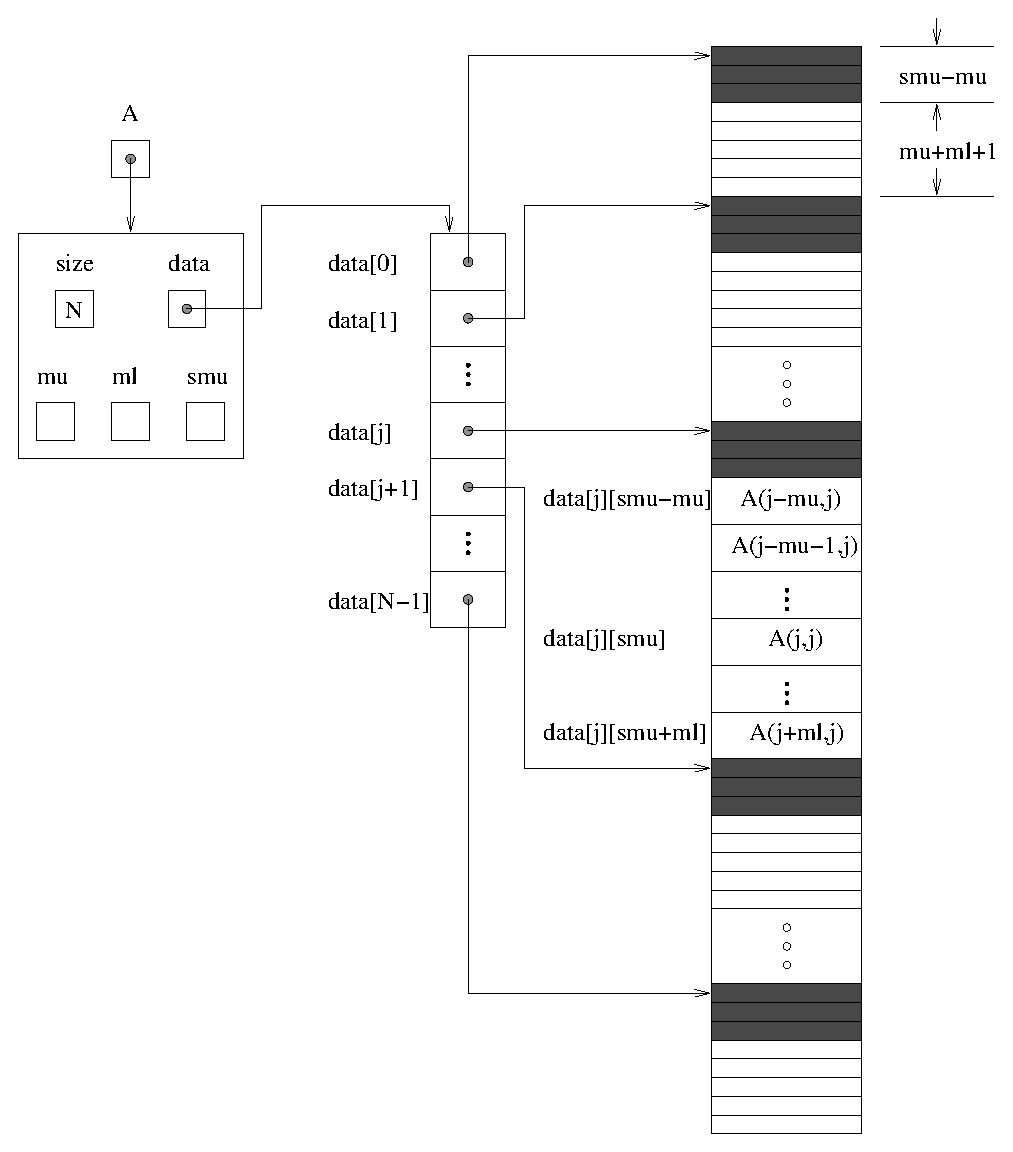
\includegraphics[width=4.5 in]{bandmat}}
\caption[Diagram of the storage for a {\sunmatband} object]
  {Diagram of the storage for the {\sunmatband} module. Here \id{A} is an
  $\id{N} \times \id{N}$ band matrix with upper and lower half-bandwidths \id{mu}
  and \id{ml}, respectively. The rows and columns of \id{A} are
  numbered from $0$ to $\id{N}-1$ and the ($i,j$)-th element of \id{A} is
  denoted \id{A(i,j)}. The greyed out areas of the underlying
  component storage are used by the associated {\sunlinsolband}
  linear solver.}\label{f:sunbandmat}
\end{figure}

\noindent The header file to include when using this module
is \id{sunmatrix/sunmatrix\_band.h}. The {\sunmatband} module
is accessible from all {\sundials} solvers \textit{without}
linking to the \newline
\id{libsundials\_sunmatrixband} module library.


% ====================================================================
\subsection{SUNMatrix\_Band accessor macros}
\label{ss:sunmat_band_macros}
% ====================================================================

The following macros are provided to access the
content of a {\sunmatband} matrix. The prefix \id{SM\_} in the names
denotes that these macros are for \emph{SUNMatrix} implementations,
and the suffix \id{\_B} denotes that these are specific to
the \emph{banded} version.
%%
\begin{itemize}

\item \ID{SM\_CONTENT\_B}

  This routine gives access to the contents of the
  banded \id{SUNMatrix}.

  The assignment \id{A\_cont} $=$ \id{SM\_CONTENT\_B(A)} sets
  \id{A\_cont} to be a pointer to the banded \id{SUNMatrix} content
  structure.

  Implementation:

  \verb|#define SM_CONTENT_B(A)     ( (SUNMatrixContent_Band)(A->content) )|

\item \ID{SM\_ROWS\_B}, \ID{SM\_COLUMNS\_B}, \ID{SM\_UBAND\_B}, \ID{SM\_LBAND\_B}, \ID{SM\_SUBAND\_B}, \ID{SM\_LDIM\_B}, and \ID{SM\_LDATA\_B}

  These macros give individual access to various lengths relevant to the
  content of a banded \id{SUNMatrix}.

  These may be used either to retrieve or to set these values.  For
  example, the assignment \id{A\_rows = SM\_ROWS\_B(A)} sets \id{A\_rows} to be
  the number of rows in the matrix \id{A}.  Similarly, the
  assignment \id{SM\_COLUMNS\_B(A) = A\_cols} sets the number of
  columns in \id{A} to equal \id{A\_cols}.

  Implementation:

  \verb|#define SM_ROWS_B(A)        ( SM_CONTENT_B(A)->M )|

  \verb|#define SM_COLUMNS_B(A)     ( SM_CONTENT_B(A)->N )|

  \verb|#define SM_UBAND_B(A)       ( SM_CONTENT_B(A)->mu )|

  \verb|#define SM_LBAND_B(A)       ( SM_CONTENT_B(A)->ml )|

  \verb|#define SM_SUBAND_B(A)      ( SM_CONTENT_B(A)->s_mu )|

  \verb|#define SM_LDIM_B(A)        ( SM_CONTENT_B(A)->ldim )|

  \verb|#define SM_LDATA_B(A)       ( SM_CONTENT_B(A)->ldata )|

\item \ID{SM\_DATA\_B} and \ID{SM\_COLS\_B}

  These macros give access to the \id{data} and \id{cols} pointers for
  the matrix entries.

  The assignment \id{A\_data = SM\_DATA\_B(A)} sets \id{A\_data} to be
  a pointer to the first component of the data array for the
  banded \id{SUNMatrix} \id{A}.  The assignment \id{SM\_DATA\_B(A) =
  A\_data} sets the data array of \id{A} to be \id{A\_data} by storing
  the pointer \id{A\_data}.

  Similarly, the assignment \id{A\_cols = SM\_COLS\_B(A)} sets \id{A\_cols} to be
  a pointer to the array of column pointers for the banded \id{SUNMatrix} \id{A}.
  The assignment \id{SM\_COLS\_B(A) = A\_cols} sets the column pointer
  array of \id{A} to be \id{A\_cols} by storing the pointer \id{A\_cols}.

  Implementation:

  \verb|#define SM_DATA_B(A)        ( SM_CONTENT_B(A)->data )|

  \verb|#define SM_COLS_B(A)        ( SM_CONTENT_B(A)->cols )|


\item \ID{SM\_COLUMN\_B}, \ID{SM\_COLUMN\_ELEMENT\_B}, and \ID{SM\_ELEMENT\_B}

  These macros give access to the individual columns and entries of
  the data array of a banded \id{SUNMatrix}.

  The assignments \id{SM\_ELEMENT\_B(A,i,j) = a\_ij} and \id{a\_ij =
  SM\_ELEMENT\_B(A,i,j)} reference the (\id{i},\id{j})-th element of the
  $\id{N} \times \id{N}$ band matrix \id{A}, where $0 \le \id{i}, \id{j} \le \id{N}-1$.
  The location (\id{i},\id{j}) should further satisfy
  \id{j}$-$\id{mu} $\le$ \id{i} $\le$ \id{j}$+$\id{ml}.

  The assignment \id{col\_j = SM\_COLUMN\_B(A,j)} sets \id{col\_j} to be
  a pointer to the diagonal element of the \id{j}-th column of the
  $\id{N} \times \id{N}$ band matrix \id{A}, $0 \le \id{j} \le \id{N}-1$.
  The type of the expression \id{SM\_COLUMN\_B(A,j)} is \id{realtype *}.
  The pointer returned by the call \id{SM\_COLUMN\_B(A,j)} can be treated as
  an array which is indexed from $-$\id{mu} to \id{ml}.

  The assignments \id{SM\_COLUMN\_ELEMENT\_B(col\_j,i,j) = a\_ij} and\\
  \id{a\_ij = SM\_COLUMN\_ELEMENT\_B(col\_j,i,j)} reference the
  (\id{i},\id{j})-th entry of the band matrix \id{A} when used in
  conjunction with \id{SM\_COLUMN\_B} to reference the \id{j}-th column
  through \id{col\_j}. The index (\id{i},\id{j}) should satisfy
  \id{j}$-$\id{mu} $\le$ \id{i} $\le$ \id{j}$+$\id{ml}.

  Implementation:

  \verb|#define SM_COLUMN_B(A,j)    ( ((SM_CONTENT_B(A)->cols)[j])+SM_SUBAND_B(A) )|

  \verb|#define SM_COLUMN_ELEMENT_B(col_j,i,j) (col_j[(i)-(j)])|

  \verb|#define SM_ELEMENT_B(A,i,j)|

  \hspace{1in} \verb|( (SM_CONTENT_B(A)->cols)[j][(i)-(j)+SM_SUBAND_B(A)] )|

\end{itemize}


% ====================================================================
\subsection{SUNMatrix\_Band functions}
\label{ss:sunmat_band_functions}
% ====================================================================

The {\sunmatband} module defines banded implementations of all matrix
operations listed in Section \ref{ss:sunmatrix_functions}. Their names are obtained
from those in Section \ref{ss:sunmatrix_functions} by appending the
suffix \id{\_Band} (e.g. \id{SUNMatCopy\_Band}).
All the standard matrix operations listed in Section \ref{ss:sunmatrix_functions} with the suffix
\id{\_Band} appended are callable via the {\F} 2003 interface by prepending an
`F' (e.g. \id{FSUNMatCopy\_Band}).

The module {\sunmatband} provides the following additional user-callable routines:
%%--------------------------------------
\sunmodfunf{SUNBandMatrix}
{
  This constructor function creates and allocates memory for a banded \id{SUNMatrix}.
  Its arguments are the matrix size, \id{N}, and the upper and lower
  half-bandwidths of the matrix, \id{mu} and \id{ml}.  The stored
  upper bandwidth is set to \id{mu+ml} to accommodate subsequent
  factorization in the {\sunlinsolband} and {\sunlinsollapband} modules.
}
{
  SUNMatrix SUNBandMatrix(sunindextype N, sunindextype mu,
  sunindextype ml)
}
%%--------------------------------------
\sunmodfun{SUNBandMatrixStorage}
{
  This constructor function creates and allocates memory for a banded \id{SUNMatrix}.
  Its arguments are the matrix size, \id{N}, the upper and lower
  half-bandwidths of the matrix, \id{mu} and \id{ml}, and the stored
  upper bandwidth, \id{smu}.  When creating a band \id{SUNMatrix},
  this value should be
  \begin{itemize}
  \item at least min(\id{N}-1,\id{mu}+\id{ml}) if the matrix will be
    used by the {\sunlinsolband} module;
  \item exactly equal to \id{mu}+\id{ml} if the matrix will be used by
    the {\sunlinsollapband} module;
  \item at least \id{mu} if used in some other manner.
  \end{itemize}
  \emph{Note: it is strongly recommended that users call the default
    constructor, \id{SUNBandMatrix}, in all standard use cases.  This
    advanced constructor is used internally within {\sundials}
    solvers, and is provided to users who require banded matrices for
    non-default purposes.}
}
{
  SUNMatrix SUNBandMatrixStorage(sunindextype N, sunindextype mu,
  \newlinefill{SUNMatrix SUNBandMatrixStorage}
  sunindextype ml, sunindextype smu)
}
%%--------------------------------------
\sunmodfun{SUNBandMatrix\_Print}
{
  This function prints the content of a banded \id{SUNMatrix} to the
  output stream specified by \id{outfile}.  Note: \id{stdout}
  or \id{stderr} may be used as arguments for \id{outfile} to print
  directly to standard output or standard error, respectively.
}
{
  void SUNBandMatrix\_Print(SUNMatrix A, FILE* outfile)
}
%%--------------------------------------
\sunmodfunf{SUNBandMatrix\_Rows}
{
  This function returns the number of rows in the banded \id{SUNMatrix}.
}
{
  sunindextype SUNBandMatrix\_Rows(SUNMatrix A)
}
%%--------------------------------------
\sunmodfunf{SUNBandMatrix\_Columns}
{
  This function returns the number of columns in the banded \id{SUNMatrix}.
}
{
  sunindextype SUNBandMatrix\_Columns(SUNMatrix A)
}
%%--------------------------------------
\sunmodfunf{SUNBandMatrix\_LowerBandwidth}
{
  This function returns the lower half-bandwidth of the banded \id{SUNMatrix}.
}
{
  sunindextype SUNBandMatrix\_LowerBandwidth(SUNMatrix A)
}
%%--------------------------------------
\sunmodfunf{SUNBandMatrix\_UpperBandwidth}
{
  This function returns the upper half-bandwidth of the banded \id{SUNMatrix}.
}
{
  sunindextype SUNBandMatrix\_UpperBandwidth(SUNMatrix A)
}
%%--------------------------------------
\sunmodfunf{SUNBandMatrix\_StoredUpperBandwidth}
{
  This function returns the stored upper half-bandwidth of the banded \id{SUNMatrix}.
}
{
  sunindextype SUNBandMatrix\_StoredUpperBandwidth(SUNMatrix A)
}
%%--------------------------------------
\sunmodfunf{SUNBandMatrix\_LDim}
{
  This function returns the length of the leading dimension of the banded \id{SUNMatrix}.
}
{
  sunindextype SUNBandMatrix\_LDim(SUNMatrix A)
}
%%--------------------------------------
\sunmodfunf{SUNBandMatrix\_Data}
{
  This function returns a pointer to the data array for the banded \id{SUNMatrix}.
}
{
  realtype* SUNBandMatrix\_Data(SUNMatrix A)
}
%%--------------------------------------
\sunmodfun{SUNBandMatrix\_Cols}
{
  This function returns a pointer to the cols array for the banded \id{SUNMatrix}.
}
{
  realtype** SUNBandMatrix\_Cols(SUNMatrix A)
}
%%--------------------------------------
\sunmodfunf{SUNBandMatrix\_Column}
{
  This function returns a pointer to the diagonal entry of the j-th
  column of the banded \id{SUNMatrix}.  The resulting pointer should
  be indexed over the range $-$\id{mu} to \id{ml}.
}
{
  realtype* SUNBandMatrix\_Column(SUNMatrix A, sunindextype j)
}
%%
%%------------------------------------
%%
\paragraph{\bf Notes}

\begin{itemize}

\item
  When looping over the components of a banded \id{SUNMatrix} \id{A},
  the most efficient approaches are to:
  \begin{itemize}
    \item First obtain the component array via \id{A\_data = SM\_DATA\_B(A)} or\\
    \id{A\_data = SUNBandMatrix\_Data(A)} and then
    access \id{A\_data[i]} within the loop.

    \item First obtain the array of column pointers via \id{A\_cols = SM\_COLS\_B(A)} or\\
    \id{A\_cols = SUNBandMatrix\_Cols(A)}, and then
    access \id{A\_cols[j][i]} within the loop.

    \item Within a loop over the columns, access the column pointer via\\
    \id{A\_colj = SUNBandMatrix\_Column(A,j)} and then to access the
    entries within that column using \id{SM\_COLUMN\_ELEMENT\_B(A\_colj,i,j)}.
  \end{itemize}
  All three of these are more efficient than
  using \id{SM\_ELEMENT\_B(A,i,j)} within a double loop.

\item
  {\warn} Within the \id{SUNMatMatvec\_Band} routine, internal
  consistency checks are performed to ensure that the matrix is called
  with consistent {\nvector} implementations.  These are currently
  limited to: {\nvecs}, {\nvecopenmp}, and {\nvecpthreads}.  As additional
  compatible vector implementations are added to {\sundials}, these
  will be included within this compatibility check.

\end{itemize}


% ====================================================================
\subsection{SUNMatrix\_Band Fortran interfaces}
\label{ss:sunmat_band_fortran}
% ====================================================================

The {\sunmatband} module provides a {\F} 2003 module as well as {\F} 77
style interface functions for use from {\F} applications.

\subsubsection*{FORTRAN 2003 interface module}
The \ID{fsunmatrix\_band\_mod} {\F} module defines interfaces to most
{\sunmatband} {\CC} functions using the intrinsic \id{iso\_c\_binding}
module which provides a standardized mechanism for interoperating with {\CC}. As
noted in the {\CC} function descriptions above, the interface functions are
named after the corresponding {\CC} function, but with a leading `F'. For
example, the function \id{SUNBandMatrix} is interfaced as
\id{FSUNBandMatrix}.

The {\F} 2003 {\sunmatband} interface module can be accessed with the \id{use}
statement, i.e. \id{use fsunmatrix\_band\_mod}, and linking to the library
\id{libsundials\_fsunmatrixband\_mod}.{\em lib} in addition to the {\CC} library.
For details on where the library and module file
\id{fsunmatrix\_band\_mod.mod} are installed see Appendix \ref{c:install}.
We note that the module is accessible from the {\F} 2003 {\sundials} integrators
\textit{without} separately linking to the
\id{libsundials\_fsunmatrixband\_mod} library.

\subsubsection*{FORTRAN 77 interface functions}
For solvers that include a {\F} interface module, the {\sunmatband}
module also includes the {\F}-callable
function \id{FSUNBandMatInit(code, N, mu, ml, ier)} to initialize
this {\sunmatband} module for a given {\sundials} solver.
Here \id{code} is an integer input solver id (1 for {\cvode}, 2 for {\ida}, 3
for {\kinsol}, 4 for {\arkode}); \id{N}, \id{mu}, and \id{ml}
are the corresponding band matrix construction arguments (declared
to match C type \id{long int}); and \id{ier} is an error return flag
equal to 0 for success and -1 for failure. Both \id{code} and \id{ier}
are declared to match C type \id{int}. Additionally, when using
{\arkode} with a non-identity mass matrix, the {\F}-callable
function \id{FSUNBandMassMatInit(N, mu, ml, ier)} initializes
this {\sunmatband} module for storing the mass matrix.

%% This is a shared SUNDIALS TEX file with a description of the
%% sparse sunmatrix implementation
%%
\section{The SUNMatrix\_Sparse implementation}\label{ss:sunmat_sparse}

The sparse implementation of the {\sunmatrix} module provided with
{\sundials}, {\sunmatsparse}, is designed to work with either
\emph{compressed-sparse-column} (CSC) or \emph{compressed-sparse-row}
(CSR) sparse matrix formats.  To this end, it defines the {\em
content} field of \id{SUNMatrix} to be the following structure:
%%
\begin{verbatim} 
struct _SUNMatrixContent_Sparse {
  sunindextype M;
  sunindextype N;
  sunindextype NNZ;
  sunindextype NP;
  realtype *data;
  int sparsetype;
  sunindextype *indexvals;
  sunindextype *indexptrs;
  /* CSC indices */
  sunindextype **rowvals;
  sunindextype **colptrs;
  /* CSR indices */
  sunindextype **colvals;
  sunindextype **rowptrs;
};
\end{verbatim}
%%
A diagram of the underlying data representation for a
CSC matrix is shown in Figure \ref{f:sparsemat} (the CSR format is
similar).  A more complete description of the parts of
this \emph{content} field is given below: 
\begin{args}[sparsetype]
  \item[M]  - number of rows
  \item[N]  - number of columns
  \item[NNZ]  - maximum number of nonzero entries in the matrix
    (allocated length of \id{data} and \id{indexvals} arrays)
  \item[NP]  - number of index pointers (e.g. number of column pointers for 
    CSC matrix). For CSC matrices $\id{NP}=\id{N}$, and for CSR
    matrices $\id{NP}=\id{M}$. This value is set automatically based
    the input for \verb|sparsetype|.
  \item[data]  - pointer to a contiguous block of \id{realtype}
    variables (of length \id{NNZ}), containing the values of the
    nonzero entries in the matrix
  \item[sparsetype]  - type of the sparse matrix (\id{CSC\_MAT} or \id{CSR\_MAT})
  \item[indexvals] - pointer to a contiguous block of \id{int} variables
    (of length \id{NNZ}), containing the row indices (if CSC) or column
   indices (if CSR) of each nonzero matrix entry held in \id{data}
  \item[indexptrs]  - pointer to a contiguous block of \id{int}
    variables (of length \id{NP+1}). For CSC matrices each 
    entry provides the index of the first column entry into the 
    \id{data} and \id{indexvals} arrays, e.g. if \id{indexptr[3]=7}, then 
    the first nonzero entry in the fourth column of the matrix is 
    located in \id{data[7]}, and is located in row \id{indexvals[7]} of the 
    matrix.  The last entry contains the total number of nonzero values in 
    the matrix and hence points one past the end of the active data in the 
    \id{data} and \id{indexvals} arrays. For CSR matrices, each entry provides 
    the index of the first row entry into the \id{data} and \id{indexvals} 
    arrays.
\end{args}
\noindent The following pointers are added to the \id{SlsMat} type for
  user convenience, to provide a more intuitive interface to the CSC
  and CSR sparse matrix data structures. They are set automatically
  when creating a sparse {\sunmatrix}, based on the sparse matrix storage
  type.  
\begin{args}[colptrs]
  \item[rowvals] - pointer to \verb|indexvals| when \id{sparsetype} is \id{CSC\_MAT},
    otherwise set to \verb|NULL|.
  \item[colptrs] - pointer to \verb|indexptrs| when \id{sparsetype} is \id{CSC\_MAT},
    otherwise set to \verb|NULL|.
  \item[colvals] - pointer to \verb|indexvals| when \id{sparsetype} is \id{CSR\_MAT},
    otherwise set to \verb|NULL|.
  \item[rowptrs] - pointer to \verb|indexptrs| when \id{sparsetype} is \id{CSR\_MAT},
    otherwise set to \verb|NULL|.
\end{args}
For example, the $5\times 4$ CSC matrix
\[
  \left[\begin{array}{cccc} 
     0 & 3 & 1 & 0\\
     3 & 0 & 0 & 2\\
     0 & 7 & 0 & 0\\
     1 & 0 & 0 & 9\\
     0 & 0 & 0 & 5
  \end{array}\right]
\]
could be stored in this structure as either
\begin{verbatim}
  M = 5;
  N = 4;
  NNZ = 8;
  NP = N;
  data = {3.0, 1.0, 3.0, 7.0, 1.0, 2.0, 9.0, 5.0};
  sparsetype = CSC_MAT;
  indexvals = {1, 3, 0, 2, 0, 1, 3, 4};
  indexptrs = {0, 2, 4, 5, 8};
\end{verbatim}
or 
\begin{verbatim}
  M = 5;
  N = 4;
  NNZ = 10;
  NP = N;
  data = {3.0, 1.0, 3.0, 7.0, 1.0, 2.0, 9.0, 5.0, *, *};
  sparsetype = CSC_MAT;
  indexvals = {1, 3, 0, 2, 0, 1, 3, 4, *, *};
  indexptrs = {0, 2, 4, 5, 8};
\end{verbatim}
where the first has no unused space, and the second has additional
storage (the entries marked with \texttt{*} may contain any values).
Note in both cases that the final value in \id{indexptrs} is $8$,
indicating the total number of nonzero entries in the matrix.

Similarly, in CSR format, the same matrix could be stored as
\begin{verbatim}
  M = 5;
  N = 4;
  NNZ = 8;
  NP = N;
  data = {3.0, 1.0, 3.0, 2.0, 7.0, 1.0, 9.0, 5.0};
  sparsetype = CSR_MAT;
  indexvals = {1, 2, 0, 3, 1, 0, 3, 3};
  indexptrs = {0, 2, 4, 5, 7, 8};
\end{verbatim}

%%
%%--------------------------------------------
%%
\begin{figure}
\centerline{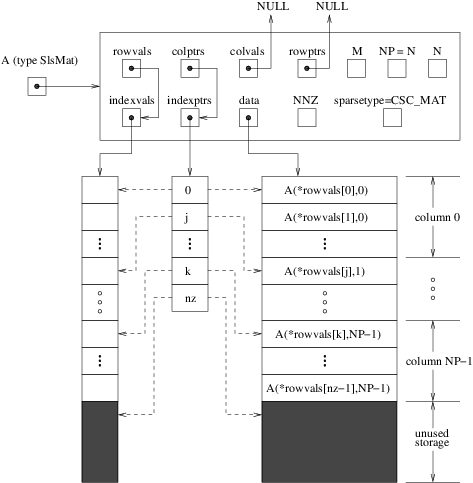
\includegraphics[width=4.5 in]{cscmat}}
\caption[Diagram of the storage for a compressed-sparse-column matrix] 
  {Diagram of the storage for a compressed-sparse-column
  matrix. Here \id{A} is an $\id{M} \times \id{N}$ sparse matrix with storage
  for up to \id{NNZ} nonzero entries (the allocated length of
  both \id{data} and \id{indexvals}).  The entries in \id{indexvals}
  may assume values from $0$ to $\id{M}-1$, corresponding to the row index
  (zero-based) of each nonzero value.  The entries in \id{data} contain
  the values of the nonzero entries, with the row $i$, column $j$
  entry of \id{A} (again, zero-based) denoted as \id{A(i,j)}.
  The \id{indexptrs} array contains $\id{N}+1$ entries; the first $\id{N}$
  denote the starting index of each column within the \id{indexvals}
  and \id{data} arrays, while the final entry points one past the
  final nonzero entry.  Here, although \id{NNZ} values are allocated,
  only \id{nz} are actually filled in; the greyed-out portions
  of \id{data} and \id{indexvals} indicate extra allocated
  space.}\label{f:sparsemat} 
\end{figure}

\noindent The header file to include when using this module 
is \id{sunmatrix/sunmatrix\_sparse.h}. The {\sunmatsparse} module
is accessible from all {\sundials} solvers \textit{without}
linking to the \\
\id{libsundials\_sunmatrixsparse} module library.


% ====================================================================
\subsection{SUNMatrix\_Sparse accessor macros}
\label{ss:sunmat_sparse_macros}
% ====================================================================

The following macros are provided to access the
content of a {\sunmatsparse} matrix. The prefix \id{SM\_} in the names
denotes that these macros are for \emph{SUNMatrix} implementations,
and the suffix \id{\_S} denotes that these are specific to
the \emph{sparse} version.
%%
\begin{itemize}

\item \ID{SM\_CONTENT\_S}
    
  This routine gives access to the contents of the
  sparse \id{SUNMatrix}.
  
  The assignment \id{A\_cont} $=$ \id{SM\_CONTENT\_S(A)} sets           
  \id{A\_cont} to be a pointer to the sparse \id{SUNMatrix} content  
  structure.                                             
                                                            
  Implementation: 
  
  \verb|#define SM_CONTENT_S(A)     ( (SUNMatrixContent_Sparse)(A->content) )|
  
\item \ID{SM\_ROWS\_S}, \ID{SM\_COLUMNS\_S}, \ID{SM\_NNZ\_S}, \ID{SM\_NP\_S}, and \ID{SM\_SPARSETYPE\_S}

  These macros give individual access to various lengths relevant to the
  content of a sparse \id{SUNMatrix}.
                                                               
  These may be used either to retrieve or to set these values.  For
  example, the assignment \id{A\_rows = SM\_ROWS\_S(A)} sets \id{A\_rows} to be
  the number of rows in the matrix \id{A}.  Similarly, the
  assignment \id{SM\_COLUMNS\_S(A) = A\_cols} sets the number of
  columns in \id{A} to equal \id{A\_cols}.
  
  Implementation: 
  
  \verb|#define SM_ROWS_S(A)        ( SM_CONTENT_S(A)->M )|

  \verb|#define SM_COLUMNS_S(A)     ( SM_CONTENT_S(A)->N )|

  \verb|#define SM_NNZ_S(A)         ( SM_CONTENT_S(A)->NNZ )|

  \verb|#define SM_NP_S(A)          ( SM_CONTENT_S(A)->NP )|

  \verb|#define SM_SPARSETYPE_S(A)  ( SM_CONTENT_S(A)->sparsetype )|


\item \ID{SM\_DATA\_S}, \ID{SM\_INDEXVALS\_S}, and \ID{SM\_INDEXPTRS\_S}
                                                            
  These macros give access to the \id{data} and index arrays for
  the matrix entries.

  The assignment \id{A\_data = SM\_DATA\_S(A)} sets \id{A\_data} to be     
  a pointer to the first component of the data array for the
  sparse \id{SUNMatrix} \id{A}.  The assignment \id{SM\_DATA\_S(A) =
  A\_data} sets the data array of \id{A} to be \id{A\_data} by storing
  the pointer \id{A\_data}. 
  
  Similarly, the assignment \id{A\_indexvals = SM\_INDEXVALS\_S(A)}
  sets \id{A\_indexvals} to be a pointer to the array of index values
  (i.e.~row indices for a CSC matrix, or column indices for a CSR
  matrix) for the sparse \id{SUNMatrix} \id{A}.  The
  assignment \id{A\_indexptrs = SM\_INDEXPTRS\_S(A)}
  sets \id{A\_indexptrs} to be a pointer to the array of index
  pointers (i.e.~the starting indices in the data/indexvals arrays for
  each row or column in CSR or CSC formats, respectively).
  
  Implementation:

  \verb|#define SM_DATA_S(A)        ( SM_CONTENT_S(A)->data )|

  \verb|#define SM_INDEXVALS_S(A)   ( SM_CONTENT_S(A)->indexvals )|

  \verb|#define SM_INDEXPTRS_S(A)   ( SM_CONTENT_S(A)->indexptrs )|

\end{itemize}


% ====================================================================
\subsection{SUNMatrix\_Sparse functions}
\label{ss:sunmat_sparse_functions}
% ====================================================================

The {\sunmatsparse} module defines sparse implementations of all matrix
operations listed in Section \ref{ss:sunmatrix_functions}. Their names are obtained
from those in Section \ref{ss:sunmatrix_functions} by appending the
suffix \id{\_Sparse} (e.g. \id{SUNMatCopy\_Sparse}). 
All the standard matrix operations listed in Section \ref{ss:sunmatrix_functions} with the suffix
\id{\_Sparse} appended are callable via the {\F} 2003 interface by prepending an
`F' (e.g. \id{FSUNMatCopy\_Sparse}).

The module {\sunmatsparse} provides the following additional
user-callable routines: 
%%--------------------------------------
\sunmodfunf{SUNSparseMatrix}
{
  This function creates and allocates memory for a sparse \id{SUNMatrix}.
  Its arguments are the number of rows and columns of the
  matrix, \id{M} and \id{N}, the maximum number of nonzeros to be
  stored in the matrix, \id{NNZ}, and a flag \id{sparsetype}
  indicating whether to use CSR or CSC format (valid arguments
  are \id{CSR\_MAT} or \id{CSC\_MAT}). 
}
{
  SUNMatrix SUNSparseMatrix(sunindextype M, sunindextype N,
  \newlinefill{SUNMatrix SUNSparseMatrix}
  sunindextype NNZ, int sparsetype)
}
%%--------------------------------------
\sunmodfunf{SUNSparseFromDenseMatrix}
{
  This function creates a new sparse matrix from an existing dense
  matrix by copying all values with magnitude larger than \id{droptol}
  into the sparse matrix structure.

  Requirements:
  \begin{itemize}
  \item \id{A} must have type \id{SUNMATRIX\_DENSE};
  \item \id{droptol} must be non-negative;
  \item \id{sparsetype} must be either \id{CSC\_MAT} or \id{CSR\_MAT}.
  \end{itemize}
  The function returns NULL if any requirements are violated, or if
  the matrix storage request cannot be satisfied. 
}
{
  SUNMatrix SUNSparseFromDenseMatrix(SUNMatrix A, realtype droptol,
  \newlinefill{SUNMatrix SUNSparseFromDenseMatrix}
  int sparsetype);
}
%%--------------------------------------
\sunmodfunf{SUNSparseFromBandMatrix}
{
  This function creates a new sparse matrix from an existing band
  matrix by copying all values with magnitude larger than \id{droptol}
  into the sparse matrix structure.

  Requirements:
  \begin{itemize}
  \item \id{A} must have type \id{SUNMATRIX\_BAND};
  \item \id{droptol} must be non-negative;
  \item \id{sparsetype} must be either \id{CSC\_MAT} or \id{CSR\_MAT}.
  \end{itemize}
  The function returns NULL if any requirements are violated, or if
  the matrix storage request cannot be satisfied. 
}
{
  SUNMatrix SUNSparseFromBandMatrix(SUNMatrix A, realtype droptol,
  \newlinefill{SUNMatrix SUNSparseFromBandMatrix}
  int sparsetype);
}
%%--------------------------------------
\sunmodfunf{SUNSparseMatrix\_Realloc}
{
  This function reallocates internal storage arrays in a sparse matrix
  so that the resulting sparse matrix has no wasted space (i.e.~the
  space allocated for nonzero entries equals the actual number of
  nonzeros, \id{indexptrs[NP]}). Returns 0 on success and 
  1 on failure (e.g.~if the input matrix is not sparse).
}
{
  int SUNSparseMatrix\_Realloc(SUNMatrix A)
}
%%--------------------------------------
\sunmodfunf{SUNSparseMatrix\_Reallocate}
{
  This function reallocates internal storage arrays in a sparse matrix
  so that the resulting sparse matrix has storage for a specified
  number of nonzeros. Returns 0 on success and 
  1 on failure (e.g.~if the input matrix is not sparse or if NNZ is
  negative). 
}
{
  int SUNSparseMatrix\_Reallocate(SUNMatrix A, sunindextype NNZ)
}
%%--------------------------------------
\sunmodfun{SUNSparseMatrix\_Print}
{
  This function prints the content of a sparse \id{SUNMatrix} to the
  output stream specified by \id{outfile}.  Note: \id{stdout}
  or \id{stderr} may be used as arguments for \id{outfile} to print
  directly to standard output or standard error, respectively.
}
{
  void SUNSparseMatrix\_Print(SUNMatrix A, FILE* outfile)
}
%%--------------------------------------
\sunmodfunf{SUNSparseMatrix\_Rows}
{
  This function returns the number of rows in the sparse \id{SUNMatrix}.
}
{
  sunindextype SUNSparseMatrix\_Rows(SUNMatrix A)
}
%%--------------------------------------
\sunmodfunf{SUNSparseMatrix\_Columns}
{
  This function returns the number of columns in the sparse \id{SUNMatrix}.
}
{
  sunindextype SUNSparseMatrix\_Columns(SUNMatrix A)
}
%%--------------------------------------
\sunmodfunf{SUNSparseMatrix\_NNZ}
{
  This function returns the number of entries allocated for nonzero
  storage for  the sparse matrix \id{SUNMatrix}.
}
{
  sunindextype SUNSparseMatrix\_NNZ(SUNMatrix A)
}
%%--------------------------------------
\sunmodfunf{SUNSparseMatrix\_NP}
{
  This function returns the number of columns/rows for the
  sparse \id{SUNMatrix}, depending on whether the matrix uses CSC/CSR
  format, respectively.  The \id{indexptrs} array has \id{NP+1} entries.
}
{
  sunindextype SUNSparseMatrix\_NP(SUNMatrix A)
}
%%--------------------------------------
\sunmodfunf{SUNSparseMatrix\_SparseType}
{
  This function returns the storage type (\id{CSR\_MAT}
  or \id{CSC\_MAT}) for the sparse \id{SUNMatrix}.
}
{
  int SUNSparseMatrix\_SparseType(SUNMatrix A)
}
%%--------------------------------------
\sunmodfunf{SUNSparseMatrix\_Data}
{
  This function returns a pointer to the data array for the
  sparse \id{SUNMatrix}. 
}
{
  realtype* SUNSparseMatrix\_Data(SUNMatrix A)
}
%%--------------------------------------
\sunmodfunf{SUNSparseMatrix\_IndexValues}
{
  This function returns a pointer to index value array for the sparse
  \id{SUNMatrix}: for CSR format this is the column index for each nonzero
  entry, for CSC format this is the row index for each nonzero entry.
}
{
  sunindextype* SUNSparseMatrix\_IndexValues(SUNMatrix A)
}
%%--------------------------------------
\sunmodfunf{SUNSparseMatrix\_IndexPointers}
{
  This function returns a pointer to the index pointer array for the
  sparse \id{SUNMatrix}: for CSR format this is the location of the first
  entry of each row in the \id{data} and \id{indexvalues} arrays, for
  CSC format this is the location of the first entry of each column.
}
{
  sunindextype* SUNSparseMatrix\_IndexPointers(SUNMatrix A)
}
%%
%%------------------------------------
%%
{\warn} Within the \id{SUNMatMatvec\_Sparse} routine, internal
consistency checks are performed to ensure that the matrix is called
with consistent {\nvector} implementations.  These are currently
limited to: {\nvecs}, {\nvecopenmp}, {\nvecpthreads}, and {\nveccuda}
when using managed memory.  As additional compatible vector implementations
are added to {\sundials}, these will be included within this compatibility check. 


% ====================================================================
\subsection{SUNMatrix\_Sparse Fortran interfaces}
\label{ss:sunmat_sparse_fortran}
% ====================================================================

The {\sunmatsparse} module provides a {\F} 2003 module as well as {\F} 77
style interface functions for use from {\F} applications.

\subsubsection*{FORTRAN 2003 interface module}
The \ID{fsunmatrix\_sparse\_mod} {\F} module defines interfaces to most
{\sunmatsparse} {\CC} functions using the intrinsic \id{iso\_c\_binding}
module which provides a standardized mechanism for interoperating with {\CC}. As
noted in the {\CC} function descriptions above, the interface functions are
named after the corresponding {\CC} function, but with a leading `F'. For
example, the function \id{SUNSparseMatrix} is interfaced as
\id{FSUNSparseMatrix}.

The {\F} 2003 {\sunmatsparse} interface module can be accessed with the \id{use}
statement, i.e. \id{use fsunmatrix\_sparse\_mod}, and linking to the library
\id{libsundials\_fsunmatrixsparse\_mod}.{\em lib} in addition to the {\CC} library.
For details on where the library and module file
\id{fsunmatrix\_sparse\_mod.mod} are installed see Appendix \ref{c:install}.
We note that the module is accessible from the {\F} 2003 {\sundials} integrators
\textit{without} separately linking to the
\id{libsundials\_fsunmatrixsparse\_mod} library.

\subsubsection*{FORTRAN 77 interface functions}
For solvers that include a Fortran interface module, the {\sunmatsparse}
module also includes the Fortran-callable
function \id{FSUNSparseMatInit(code, M, N, NNZ, sparsetype, ier)} to
initialize this {\sunmatsparse} module for a given {\sundials} solver.
Here \id{code} is an integer input for the solver id (1 for {\cvode},
2 for {\ida}, 3 for {\kinsol}, 4 for {\arkode}); \id{M}, \id{N}
and \id{NNZ} are the corresponding sparse matrix construction
arguments (declared to match C type \id{long
int}); \id{sparsetype} is an integer flag indicating the sparse
storage type (0 for CSC, 1 for CSR); and \id{ier} is an error return
flag equal to 0 for success and -1 for failure. Each of \id{code},
\id{sparsetype} and \id{ier} are declared so as to match C
type \id{int}. Additionally, when using {\arkode} with a non-identity
mass matrix, the Fortran-callable
function \id{FSUNSparseMassMatInit(M, N, NNZ, sparsetype, ier)} 
initializes this {\sunmatsparse} module for storing the mass matrix.

%% This is a shared SUNDIALS TEX file with a description of the
%% SuperLU_DIST SLUNRloc SUNMatrix implementation
%%
\section{The SUNMatrix\_SLUNRloc implementation}\label{ss:sunmat_slunrloc}

The {\sunmatslunrloc} implementation of the {\sunmatrix} module provided with
{\sundials} is an adapter for the \id{SuperMatrix} structure provided by the
{\superludist} sparse matrix factorization and solver library written by
X. Sherry Li \cite{SuperLUDIST_site,GDL:07,LD:03,SLUUG:99}.
It is designed to be used with the {\sunlinsolsludist} linear solver
discussed in Section~\ref{ss:sunlinsol_sludist}. To this end, it defines the
{\em content} field of \id{SUNMatrix} to be the following structure:
%%
\begin{verbatim}
struct _SUNMatrixContent_SLUNRloc {
  booleantype   own_data;
  gridinfo_t    *grid;
  sunindextype  *row_to_proc;
  pdgsmv_comm_t *gsmv_comm;
  SuperMatrix   *A_super;
  SuperMatrix   *ACS_super;
};
\end{verbatim}
%%

A more complete description of the this \emph{content} field is given below:

\begin{description}
  \item[own\_data] - a flag which indicates if the SUNMatrix is responsible for freeing
    \id{A\_super}
  \item[grid] - pointer to the {\superludist} structure that stores the 2D process grid
  \item[row\_to\_proc] - a mapping between the rows in the matrix and the process it
    resides on; will be \id{NULL} until the \id{SUNMatMatvecSetup} routine is called
  \item[gsmv\_comm] - pointer to the {\superludist} structure that stores the
    communication information needed for matrix-vector multiplication; will be
    \id{NULL} until the \id{SUNMatMatvecSetup} routine is called
  \item[A\_super] - pointer to the underlying {\superludist} \id{SuperMatrix} with
      \id{Stype = SLU\_NR\_loc, Dtype = SLU\_D, Mtype = SLU\_GE}; must have the
      full diagonal present to be used with \id{SUNMatScaleAddI} routine
  \item[ACS\_super] - a column-sorted version of the matrix needed to perform matrix-vector
    multiplication; will be \id{NULL} until the routine \id{SUNMatMatvecSetup}
    routine is called
\end{description}

\noindent The header file to include when using this module
is \id{sunmatrix/sunmatrix\_slunrloc.h}. The installed module
library to link to is \id{libsundials\_sunmatrixslunrloc.\textit{lib}}
where \id{\em.lib} is typically \id{.so} for shared libraries and
\id{.a} for static libraries.


% ====================================================================
\subsection{SUNMatrix\_SLUNRloc functions}
\label{ss:sunmat_slunrloc_functions}
% ====================================================================

The module {\sunmatslunrloc} provides the following user-callable routines:
%%--------------------------------------
%%
\ucfunction{SUNMatrix\_SLUNRloc}
{
  A = SUNMatrix\_SLUNRloc(Asuper, grid);
}
{
  The function \ID{SUNMatrix\_SLUNRloc} creates and allocates memory for a
  {\sunmatslunrloc} object.
}
{
  \begin{args}
  \item[Asuper] (\id{SuperMatrix*})
      a fully-allocated {\superludist} \id{SuperMatrix} that the SUNMatrix will
      wrap; must have \id{Stype = SLU\_NR\_loc, Dtype = SLU\_D, Mtype = SLU\_GE}
      to be compatible
  \item[grid] (\id{gridinfo\_t*}) the initialized {\superludist} 2D process grid structure
  \end{args}
}
{
  a \id{SUNMatrix} object if \id{Asuper} is compatible else \id{NULL}
}
{
}

\ucfunction{SUNMatrix\_SLUNRloc\_Print}
{
  SUNMatrix\_SLUNRloc\_Print(A, fp);
}
{
  The function \ID{SUNMatrix\_SLUNRloc\_Print} prints the underlying
  \id{SuperMatrix} content.
}
{
  \begin{args}
  \item[A] (\id{SUNMatrix}) the matrix to print
  \item[fp] (\id{FILE}) the file pointer used for printing
  \end{args}
}
{
  \id{void}
}
{
}

\ucfunction{SUNMatrix\_SLUNRloc\_SuperMatrix}
{
  Asuper = SUNMatrix\_SLUNRloc\_SuperMatrix(A);
}
{
  The function \ID{SUNMatrix\_SLUNRloc\_SuperMatrix} provides access
  to the underlying {\superludist} \id{SuperMatrix} of \id{A}.
}
{
  \begin{args}
  \item[A] (\id{SUNMatrix}) the matrix to access
  \end{args}
}
{
  \id{SuperMatrix*}
}
{
}

\ucfunction{SUNMatrix\_SLUNRloc\_ProcessGrid}
{
  grid = SUNMatrix\_SLUNRloc\_ProcessGrid(A);
}
{
  The function \ID{SUNMatrix\_SLUNRloc\_ProcessGrid} provides access
  to the {\superludist} \id{gridinfo\_t} structure associated with \id{A}.
}
{
  \begin{args}
  \item[A] (\id{SUNMatrix}) the matrix to access
  \end{args}
}
{
  \id{gridinfo\_t*}
}
{
}

\ucfunction{SUNMatrix\_SLUNRloc\_OwnData}
{
  does\_own\_data = SUNMatrix\_SLUNRloc\_OwnData(A);
}
{
  The function \ID{SUNMatrix\_SLUNRloc\_OwnData} returns true if the \id{SUNMatrix}
  object is responsible for freeing \id{A\_super}, otherwise it returns false.
}
{
  \begin{args}
  \item[A] (\id{SUNMatrix}) the matrix to access
  \end{args}
}
{
  \id{booleantype}
}
{
}

The {\sunmatslunrloc} module defines implementations of all generic \id{SUNMatrix} operations
listed in Section \ref{ss:sunmatrix_functions}:

\begin{itemize}
  \item \id{SUNMatGetID\_SLUNRloc} - returns \id{SUNMATRIX\_SLUNRLOC}
  \item \id{SUNMatClone\_SLUNRloc}
  \item \id{SUNMatDestroy\_SLUNRloc}
  \item \id{SUNMatSpace\_SLUNRloc} - this only returns information for the storage within the
    matrix interface, i.e. storage for \id{row\_to\_proc}
  \item \id{SUNMatZero\_SLUNRloc}
  \item \id{SUNMatCopy\_SLUNRloc}
  \item \id{SUNMatScaleAdd\_SLUNRloc} - performs $A = cA + B$, but $A$ and $B$ must have the same sparsity pattern 
  \item \id{SUNMatScaleAddI\_SLUNRloc} - performs $A = cA + I$, but the diagonal of $A$ must be present
  \item \id{SUNMatMatvecSetup\_SLUNRloc} - initializes the {\superludist} parallel communication
    structures needed to perform a matrix-vector product; only needs to be called before the
    first call to \id{SUNMatMatvec} or if the matrix changed since the last setup
  \item \id{SUNMatMatvec\_SLUNRloc}
\end{itemize}

%%------------------------------------
%%
{\warn} The {\sunmatslunrloc} module requires that the complete diagonal, i.e. nonzeros and zeros,
is present in order to use the \id{SUNMatScaleAddI} operation.

% % ====================================================================
% \subsection{SUNMatrix\_SLUNRloc Fortran interfaces}
% \label{ss:sunmat_slunrloc_fortran}
% % ====================================================================

% The {\sunmatslunrloc} module provides a {\F} 2003 module as well as {\F} 77
% style interface functions for use from {\F} applications.

% \subsubsection*{FORTRAN 2003 interface module}
% The \ID{fsunmatrix\_slunrloc\_mod} {\F} module defines interfaces to most
% {\sunmatslunrloc} {\CC} functions using the intrinsic \id{iso\_c\_binding}
% module which provides a standardized mechanism for interoperating with {\CC}. As
% noted in the {\CC} function descriptions above, the interface functions are
% named after the corresponding {\CC} function, but with a leading `F'. For
% example, the function \id{SUNMatrix\_SLUNRloc} is interfaced as
% \id{FSUNMatrix\_SLUNRloc}.

% The {\F} 2003 {\sunmatslunrloc} interface module can be accessed with the \id{use}
% statement, i.e. \id{use fsunmatrix\_slunrloc\_mod}, and linking to the library
% \id{libsundials\_fsunmatrixslunrloc\_mod}.{\em lib} in addition to the {\CC} library.
% For details on where the library and module file \id{fsunmatrix\_slunrloc\_mod.mod}
% are installed see Appendix \ref{c:install}.


%% This is a shared SUNDIALS TEX file with a description of the
%% cuSPARSE SUNMatrix implementation.
%%
\section{The SUNMatrix\_cuSparse implementation}\label{ss:sunmat_cusparse}

The \id{SUNMATRIX\_CUSPARSE} implementation of the \id{SUNMatrix} module provided with
{\sundials}, is an interface to the NVIDIA cuSPARSE matrix for use on NVIDIA GPUs
\cite{cuSPARSE_site}. All data stored by this matrix implementation resides on the
GPU at all times. The implementation currently supports the cuSPARSE CSR matrix
format described in the cuSPARSE documentation as well as a unique low-storage
format for block-diagonal matrices of the form
\begin{equation*}
  \mathbf{A} =
  \begin{bmatrix}
    \mathbf{A_0} & 0 & \cdots & 0\\
    0 & \mathbf{A_1} & \cdots & 0\\
    \vdots & \vdots & \ddots & \vdots\\
    0 & 0 & \cdots & \mathbf{A_{n-1}}\\
  \end{bmatrix}
\end{equation*}
where all the block matrices $A_j$ share the same sparsity pattern.
We will refer to this format as BCSR (not to be confused with the canonical BSR format where
each block is stored as dense). In this format, the CSR column indices and row pointers
are only stored for the first block and are computed only as necessary for other blocks.
This can drastically reduce the amount of storage required compared to the regular CSR
format when there is a large number of blocks. This format is well-suited for, and
intended to be used with the \id{SUNLinearSolver\_cuSolverSp\_batchQR} linear
solver (see Section \ref{ss:sunlinsol_cuspbqr}).

The header file to include when using this module is
\id{sunmatrix/sunmatrix\_cusparse.h}. The installed library to link to is
\id{libsundials\_sunmatrixcusparse.\textit{lib}} where \id{\em.lib} is typically \id{.so}
for shared libraries and \id{.a} for static libraries.
\newline
\newline
{\warn}The \id{SUNMatrix\_cuSparse} module is experimental and subject to change.

% ====================================================================
\subsection{SUNMatrix\_cuSparse functions}
\label{ss:sunmat_cusparse_functions}
% ====================================================================

The \id{SUNMATRIX\_CUSPARSE} module defines GPU-enabled sparse implementations
of all matrix operations listed in Section
\ref{ss:sunmatrix_functions} except for the \id{SUNMatSpace}
and \id{SUNMatMatvecSetup} operations:

\begin{enumerate}
  \item \id{SUNMatGetID\_cuSparse} -- returns \id{SUNMATRIX\_CUSPARSE}
  \item \id{SUNMatClone\_cuSparse}
  \item \id{SUNMatDestroy\_cuSparse}
  \item \id{SUNMatZero\_cuSparse}
  \item \id{SUNMatCopy\_cuSparse}
  \item \id{SUNMatScaleAdd\_cuSparse} -- performs $A = cA + B$, where $A$ and $B$
    must have the same sparsity pattern
  \item \id{SUNMatScaleAddI\_cuSparse} -- performs $A = cA + I$, where the diagonal
    of $A$ must be present
  \item \id{SUNMatMatvec\_cuSparse}
\end{enumerate}


In addition, the SUNMATRIX\_CUSPARSE module defines the following implementation specific
functions:

%%--------------------------------------
%%
\ucfunction{SUNMatrix\_cuSparse\_NewCSR}
{
  A = SUNMatrix\_cuSparse\_NewCSR(M, N, NNZ, cusp)
}
{
  This constructor function creates and allocates memory for a \id{SUNMATRIX\_CUSPARSE}
  \id{SUNMatrix} that uses the CSR storage format.
}
{
  \begin{args}[cusp]
  \item[M] (\id{int}) the number of matrix rows
  \item[N] (\id{int}) the number of matrix columns
  \item[NNZ] (\id{int}) the number of matrix nonzeros
  \item[cusp] (\id{cusparseHandle\_t}) a valid \id{cusparseHandle\_t}
  \end{args}
}
{
  a \id{SUNMatrix} object if successful else \id{NULL}
}
{}

%%--------------------------------------
%%
\ucfunction{SUNMatrix\_cuSparse\_NewBlockCSR}
{
  A = SUNMatrix\_cuSparse\_NewBlockCSR(nblocks, blockrows, blockcols, blocknnz, cusp)
}
{
  This constructor function creates and allocates memory for a \id{SUNMATRIX\_CUSPARSE}
  \id{SUNMatrix} that leverages the \id{SUNMAT\_CUSPARSE\_BCSR} storage
  format to store a block diagonal matrix where each block shares the same
  sparsity pattern. \textbf{The blocks must be square.}
}
{
  \begin{args}[blockcols]
  \item[nblocks] (\id{int}) the number of matrix blocks
  \item[blockrows] (\id{int}) the number of rows for a block
  \item[blockcols] (\id{int}) the number of columns for a block
  \item[blocknnz] (\id{int}) the number of nonzeros in a block
  \item[cusp] a valid \id{cusparseHandle\_t}
  \end{args}
}
{
  a \id{SUNMatrix} object if successful else \id{NULL}
}
{
  The \id{SUNMAT\_CUSPARSE\_BCSR} format currently only supports square matrices.
}

%%--------------------------------------
%%
\ucfunction{SUNMatrix\_cuSparse\_MakeCSR}
{
  A = SUNMatrix\_cuSparse\_MakeCSR(mat\_descr, M, N, NNZ, rowptrs, colind, data, cusp)
}
{
  This constructor function creates and allocates memory for a \id{SUNMATRIX\_CUSPARSE}
  \id{SUNMatrix} that uses the CSR storage format from the user provided pointers.
}
{
  \begin{args}[mat\_decsr]
  \item[mat\_decsr] a valid \id{cusparseMatDescr\_t} object;
    must use \id{CUSPARSE\_INDEX\_BASE\_ZERO} indexing
  \item[M] (\id{int}) the number of matrix rows
  \item[N] (\id{int}) the number of matrix columns
  \item[NNZ] (\id{int}) the number of matrix nonzeros
  \item[rowptrs] (\id{int*})a contiguous array of the CSR row pointers
  \item[colind] (\id{int*}) a contiguous array of the CSR column indices
  \item[data] (\id{realtype*}) a contiguous array of the nonzero data
  \item[cusp] (\id{cusparseHandle\_t}) a valid \id{cusparseHandle\_t}
  \end{args}
}
{
  a \id{SUNMatrix} object if successful else \id{NULL}
}
{}

%%--------------------------------------
%%
\ucfunction{SUNMatrix\_cuSparse\_Rows}
{
  M = SUNMatrix\_cuSparse\_Rows(A)
}
{
  This function returns the number of rows in the sparse \id{SUNMatrix}.
}
{
  \begin{args}
  \item[A] (\id{SUNMatrix})
  \end{args}
}
{
  the number of rows in the sparse \id{SUNMatrix}
}
{}

%%--------------------------------------
%%
\ucfunction{SUNMatrix\_cuSparse\_Columns}
{
  N = SUNMatrix\_cuSparse\_Columns(A)
}
{
  This function returns the number of columns in the sparse \id{SUNMatrix}.
}
{
  \begin{args}
  \item[A] (\id{SUNMatrix})
  \end{args}
}
{
  the number of columns in the sparse \id{SUNMatrix}
}
{}

%%--------------------------------------
%%
\ucfunction{SUNMatrix\_cuSparse\_NNZ}
{
  nnz = SUNMatrix\_cuSparse\_NNZ(A)
}
{
  This function returns the number of nonzeros in the sparse \id{SUNMatrix}.
}
{
  \begin{args}
  \item[A] (\id{SUNMatrix})
  \end{args}
}
{
  the number of nonzeros in the sparse \id{SUNMatrix}
}
{}

%%--------------------------------------
%%
\ucfunction{SUNMatrix\_cuSparse\_SparseType}
{
  type = SUNMatrix\_cuSparse\_SparseType(A)
}
{
  This function returns the sparsity format for the sparse \id{SUNMatrix}.
}
{
  \begin{args}
  \item[A] (\id{SUNMatrix})
  \end{args}
}
{
  the \id{SUNMAT\_CUSPARSE\_CSR} or \id{SUNMAT\_CUSPARSE\_BCSR} sparsity formats
}
{}

%%--------------------------------------
%%
\ucfunction{SUNMatrix\_cuSparse\_IndexValues}
{
  colind = SUNMatrix\_cuSparse\_IndexValues(A)
}
{
  This function returns a pointer to the index value array for the sparse
  \id{SUNMatrix}.
}
{
  \begin{args}
  \item[A] (\id{SUNMatrix})
  \end{args}
}
{
  for the CSR format this is an array of the column indices for each nonzero
  entry. For the BCSR format this is an array of the column indices
  for each nonzero entry in the first block only.
}
{}

%%--------------------------------------
%%
\ucfunction{SUNMatrix\_cuSparse\_IndexPointers}
{
  rowptrs = SUNMatrix\_cuSparse\_IndexPointers(A)
}
{
  This function returns a pointer to the index pointers array for the
  sparse \id{SUNMatrix}.
}
{
  \begin{args}
  \item[A] (\id{SUNMatrix})
  \end{args}
}
{
  for the CSR format this is an array of the locations
  of the first entry of each row in the \id{data} and \id{indexvalues} arrays,
  for the BCSR format this is an array of the locations of each row in the
  \id{data} and \id{indexvalues} arrays in the first block only.
}
{}

%%--------------------------------------
%%
\ucfunction{SUNMatrix\_cuSparse\_NumBlocks}
{
  nblocks = SUNMatrix\_cuSparse\_NumBlocks(A)
}
{
  This function returns the number of blocks in the sparse \id{SUNMatrix}.
}
{
  \begin{args}
  \item[A] (\id{SUNMatrix})
  \end{args}
}
{
  the number of matrix blocks
}
{}


%%--------------------------------------
%%
\ucfunction{SUNMatrix\_cuSparse\_BlockRows}
{
  blockrows = SUNMatrix\_cuSparse\_BlockRows(A)
}
{
  This function returns the number of rows of a
  block of the sparse \id{SUNMatrix}.
}
{
  \begin{args}
  \item[A] (\id{SUNMatrix})
  \end{args}
}
{
  the number of rows of a block
}
{}


%%--------------------------------------
%%
\ucfunction{SUNMatrix\_cuSparse\_BlockColumns}
{
  blockrows = SUNMatrix\_cuSparse\_BlockColumns(A)
}
{
  This function returns the number of columns of a
  block of the sparse \id{SUNMatrix}.
}
{
  \begin{args}
  \item[A] (\id{SUNMatrix})
  \end{args}
}
{
  the number of columns of a block
}
{}


%%--------------------------------------
%%
\ucfunction{SUNMatrix\_cuSparse\_BlockNNZ}
{
  blockdim = SUNMatrix\_cuSparse\_BlockNNZ(A)
}
{
  This function returns the nonzeros of a block of the sparse \id{SUNMatrix}.
}
{
  \begin{args}
  \item[A] (\id{SUNMatrix})
  \end{args}
}
{
  the number of nonzeros of a block
}
{}

%%--------------------------------------
%%
\ucfunction{SUNMatrix\_cuSparse\_BlockData}
{
  nzdata = SUNMatrix\_cuSparse\_BlockData(A, blockidx)
}
{
  This function returns a pointer to the start of the nonzero values
  in the data array for given block index. The first block in the
  \id{SUNMatrix} is index 0, the second block is index 1, and so on.
}
{
  \begin{args}
  \item[A] (\id{SUNMatrix})
  \item[blockidx] (\id{int}) the index of the desired block
  \end{args}
}
{
  a pointer to the start of the nonzero values in the data array for given
  block index
}
{}

%%--------------------------------------
%%
\ucfunction{SUNMatrix\_cuSparse\_CopyToDevice}
{
  retval = SUNMatrix\_cuSparse\_CopyToDevice(A, h\_data, h\_idxptrs, h\_idxvals)
}
{
  This functions copies the matrix information to the GPU device from the provided
  host arrays.  A user may provide \id{NULL} for any of \id{h\_data}, \id{h\_idxptrs}, or
  \id{h\_idxvals} to avoid copying that information.
}
{
  \begin{args}[h\_idxptrs]
  \item[A] (\id{SUNMatrix})
  \item[h\_data] (\id{realtype*}) a pointer to an allocated array of
    at least \id{SUNMatrix\_cuSparse\_NNZ(A)} \id{*} \id{sizeof(realtype)}
    bytes; the nonzero values will be copied from this array onto the device
  \item[h\_idxptrs] (\id{int*}) a pointer to an allocated array of
    at least \id{(SUNMatrix\_cuSparse\_BlockDim(A)+1)} \id{*} \id{sizeof(int)}
    bytes; the index pointers will be copied from this array onto the device
  \item[h\_idxvals] (\id{int*}) a pointer to an allocated array of
    at least \id{SUNMatrix\_cuSparse\_BlockNNZ(A)} \id{*} \id{sizeof(int)}
    bytes; the index values will be copied from this array onto the device
  \end{args}
}
{
  \id{SUNMAT\_SUCCESS} if the copy operation(s) were successful, or a nonzero error
  code otherwise.
}
{}

%%--------------------------------------
%%
\ucfunction{SUNMatrix\_cuSparse\_CopyFromDevice}
{
  retval = SUNMatrix\_cuSparse\_CopyFromDevice(A, h\_data, h\_idxptrs, h\_idxvals)
}
{
  This functions copies the matrix information from the GPU device to the provided
  host arrays. A user may provide \id{NULL} for any of \id{h\_data}, \id{h\_idxptrs}, or
  \id{h\_idxvals} to avoid copying that information.
}
{
  \begin{args}[h\_idxptrs]
  \item[A] (\id{SUNMatrix})
  \item[h\_data] (\id{realtype*}) a pointer to an allocated array of
    at least \id{SUNMatrix\_cuSparse\_NNZ(A)} \id{*} \id{sizeof(realtype)}
    bytes; the nonzero values will be copied into this array from the device
  \item[h\_idxptrs] (\id{int*}) a pointer to an allocated array of
    at least \id{(SUNMatrix\_cuSparse\_BlockDim(A)+1)} \id{*} \id{sizeof(int)}
    bytes; the index pointers will be copied into this array from the device
  \item[h\_idxvals] (\id{int*}) a pointer to an allocated array of
    at least \id{SUNMatrix\_cuSparse\_BlockNNZ(A)} \id{*} \id{sizeof(int)}
    bytes; the index values will be copied into this array from the device
  \end{args}
}
{
  \id{SUNMAT\_SUCCESS} if the copy operation(s) were successful, or a nonzero error
  code otherwise.
}
{}

%%--------------------------------------
%%
\ucfunction{SUNMatrix\_cuSparse\_SetKernelExecPolicy}
{
  retval = SUNMatrix\_cuSparse\_SetKernelExecPolicy(A, exec\_policy);
}
{
  This function sets the execution policies which control the kernel parameters
  utilized when launching the CUDA kernels. By default the matrix is setup to use
  a policy which tries to leverage the structure of the matrix. See section
  \ref{ss:suncudaexecpolicy} for more information about the \id{SUNCudaExecPolicy}
  class.
}
{
  \begin{args}[exec\_policy]
    \item[A] (\id{SUNMatrix})
    \item[exec\_policy] (\id{SUNCudaExecPolicy*})
  \end{args}
}
{
  \id{SUNMAT\_SUCCESS} if the operation(s) were successful, or a nonzero error
  code otherwise.
}
{
  All matrices and vector used in a single instance of a {\sundials} solver must
  use the same {\cuda} stream, and the {\cuda} stream must be set prior to
  solver initialization.
}

%%--------------------------------------
%%
\ucfunction{SUNMatrix\_cuSparse\_SetFixedPattern}
{
  retval = SUNMatrix\_cuSparse\_SetFixedPattern(A, yesno)
}
{
  This function changes the behavior of the the \id{SUNMatZero} operation on
  the \id{SUNMatrix} object \id{A}. By default the matrix sparsity pattern
  is not considered to be fixed, thus, the \id{SUNMatZero} operation zeros out
  all \id{data} array as well as the \id{indexvalues} and \id{indexpointers} arrays.
  Providing a value of \id{1} or \id{SUNTRUE} for the  \id{yesno} argument changes
  the behavior of \id{SUNMatZero} on \id{A} so that only the data is zeroed out, but
  not the \id{indexvalues} or \id{indexpointers} arrays. Providing a value of \id{0}
  or \id{SUNFALSE} for the \id{yesno} argument is equivalent to the default behavior.
}
{
  \begin{args}[yesno]
  \item[A] (\id{SUNMatrix})
  \item[yesno] (\id{booleantype})
  \end{args}
}
{
  \id{SUNMAT\_SUCCESS} if the operation(s) were successful, or a nonzero error
  code otherwise.
}
{}

% ====================================================================
\subsection{SUNMatrix\_cuSparse Usage Notes}
\label{ss:sunmat_cusparse_notes}
% ====================================================================

The \id{SUNMATRIX\_CUSPARSE} module only supports 32-bit indexing,
thus {\sundials} must be built for 32-bit indexing to use this module.

The \id{SUNMATRIX\_CUSPARSE} module can be used with CUDA streams by
calling the cuSPARSE function \id{cusparseSetStream} on the the
\id{cusparseHandle\_t} that is provided to the \id{SUNMATRIX\_CUSPARSE}
constructor.

{\warn} When using the \id{SUNMATRIX\_CUSPARSE} module with a {\sundials}
package (e.g. {\cvode}), the stream given to cuSPARSE should be the same
stream used for the {\nvector} object that is provided to the package,
and the {\nvector} object given to the \id{SUNMatvec} operation. If different
streams are utilized, synchronization issues may occur.


\clearemptydoublepage
%===============================================================
% Description of the SUNLinearSolver Concept
%===================================================================================
\chapter{Description of the SUNLinearSolver module}\label{s:sunlinsol}
%===================================================================================
\index{SUNLinearSolver@\texttt{SUNLinearSolver} module}
% This is a shared SUNDIALS TEX file with description of
% the generic sunlinsol abstraction
%
For problems that involve the solution of linear systems of equations,
the {\sundials} packages operate using generic linear solver modules
defined through the {\sunlinsol} API.  This allows {\sundials}
packages to utilize any valid {\sunlinsol} implementation that provides
a set of required functions.  These functions can be divided into
three categories.  The first are the core linear solver functions.  The
second group consists of ``set'' routines to supply the linear solver object
with functions provided by the {\sundials} package, or for modification
of solver parameters.  The last group consists of ``get'' routines for
retrieving artifacts (statistics, residual vectors, etc.) from the
linear solver.  All of these functions are defined in the header file
\Id{sundials/sundials\_linearsolver.h}.

The implementations provided with {\sundials} work in coordination
with the {\sundials} generic {\nvector} and {\sunmatrix} modules to
provide a set of compatible data structures and solvers for the
solution of linear systems using direct or iterative (matrix-based or matrix-free)
methods.  Moreover, advanced users can provide a customized
\Id{SUNLinearSolver} implementation to any {\sundials} package,
particularly in cases where they provide their own {\nvector} and/or
{\sunmatrix} modules.

Historically, the {\sundials} packages have been designed to specifically
leverage the use of either \emph{direct linear solvers} or matrix-free,
\emph{scaled, preconditioned, iterative linear solvers}.  However,
matrix-based iterative linear solvers are also supported.

The iterative linear solvers packaged with {\sundials} leverage
scaling and preconditioning, as applicable, to balance error between
solution components and to accelerate convergence of the linear
solver.  To this end, instead of solving the  linear system $Ax = b$
directly, these apply the underlying iterative algorithm to the
transformed system
\begin{equation}
  \label{eq:transformed_linear_system}
  \tilde{A} \tilde{x} = \tilde{b}
\end{equation}
where
\begin{align}
  \notag
  \tilde{A} &= S_1 P_1^{-1} A P_2^{-1} S_2^{-1},\\
  \label{eq:transformed_linear_system_components}
  \tilde{b} &= S_1 P_1^{-1} b,\\
  \notag
  \tilde{x} &= S_2 P_2 x,
\end{align}
and where
\begin{itemize}
\item $P_1$ is the left preconditioner,
\item $P_2$ is the right preconditioner,
\item $S_1$ is a diagonal matrix of scale factors for $P_1^{-1} b$,
\item $S_2$ is a diagonal matrix of scale factors for $P_2 x$.
\end{itemize}
The scaling matrices are chosen so that $S_1 P_1^{-1} b$ and $S_2 P_2 x$
have dimensionless components. If preconditioning is done on the left only
($P_2 = I$), by a  matrix $P$, then $S_2$ must be a scaling for $x$, while $S_1$
is a scaling for $P^{-1} b$, and so may also be taken as a scaling for $x$.
Similarly, if preconditioning is done on the right only ($P_1 = I$ and
$P_2 = P$), then $S_1$ must be a scaling for $b$, while $S_2$ is a scaling for
$P x$, and may also be taken as a scaling for $b$.

{\sundials} packages request that iterative linear solvers stop
based on the 2-norm of the scaled preconditioned residual meeting a
prescribed tolerance
\[
  \left\| \tilde{b} - \tilde{A} \tilde{x} \right\|_2  <  \text{tol}.
\]

When provided an iterative {\sunlinsol} implementation that does not
support the scaling matrices $S_1$ and $S_2$, {\sundials}'
packages will adjust the value of $\text{tol}$ accordingly
(see \S\ref{ss:sunlinsol_iterative_tolerance} for more details). In
this case, they instead request that iterative linear solvers stop
based on the criteria
\[
   \left\| P_1^{-1} b - P_1^{-1} A x \right\|_2  <  \text{tol}.
\]
We note that the corresponding adjustments to $\text{tol}$ in
this case are non-optimal, in that they cannot balance error between
specific entries of the solution $x$, only the aggregate error
in the overall solution vector.

We further note that not all of the {\sundials}-provided iterative
linear solvers support the full range of the above options (e.g.,
separate left/right preconditioning), and that some of the {\sundials}
packages only utilize a subset of these options.  Further details on
these exceptions are described in the documentation for each
{\sunlinsol} implementation, or for each {\sundials} package.

For users interested in providing their own {\sunlinsol} module, the
following section presents the {\sunlinsol} API and its implementation
beginning with the definition of {\sunlinsol} functions in sections
\ref{ss:sunlinsol_CoreFn} -- \ref{ss:sunlinsol_GetFn}. This is followed by
the definition of functions supplied to a linear solver implementation in
section \ref{ss:sunlinsol_SUNSuppliedFn}. A table of linear solver return
codes is given in section \ref{ss:sunlinsol_ErrorCodes}. The
\id{SUNLinearSolver} type and the generic {\sunlinsol} module are defined
in section \ref{ss:sunlinsol_Generic}.  The section
\ref{ss:sunlinsol_compatibility} discusses compatibility between the
{\sundials}-provided {\sunlinsol} modules and {\sunmatrix} modules.
Section \ref{ss:sunlinsol_custom} lists the requirements for supplying a custom
{\sunlinsol} module and discusses some intended use cases. Users wishing to
supply their own {\sunlinsol} module are encouraged to use the {\sunlinsol}
implementations provided with {\sundials} as a template for supplying custom
linear solver modules. The {\sunlinsol} functions required by this {\sundials}
package as well as other package specific details are given in
section \ref{s:sunlinsol_interface}. The remaining sections of this chapter
present the {\sunlinsol} modules provided with {\sundials}.

% ====================================================================
\section{The SUNLinearSolver API}
\label{s:sunlinsol_api}
% ====================================================================

The {\sunlinsol} API defines several linear solver operations that enable
{\sundials} packages to utilize any {\sunlinsol} implementation that
provides the required functions. These functions can be divided into three
categories. The first are the core linear solver functions. The second group
of functions consists of set routines to supply the linear solver with
functions provided by the {\sundials} time integrators and to modify solver
parameters. The final group consists of get routines for retrieving linear
solver statistics. All of these functions are defined in the header file
\id{sundials/sundials\_linearsolver.h}.



%---------------------------------------------------------------------------
\subsection{\id{SUNLinearSolver} core functions}\label{ss:sunlinsol_CoreFn}

The core linear solver functions consist of two required functions to get the
linear solver type \\ \noindent (\Id{SUNLinSolGetType}) and solve the linear
system $Ax=b$ (\Id{SUNLinSolSolve}). The remaining functions are for getting the
solver ID (\Id{SUNLinSolGetID}), initializing the linear solver object once all
solver-specific options have been set (\Id{SUNLinSolInitialize}), setting up the
linear solver object to utilize an updated matrix $A$ (\Id{SUNLinSolSetup}), and
for destroying the linear solver object (\Id{SUNLinSolFree}) are optional.

% --------------------------------------------------------------------
\ucfunctionf{SUNLinSolGetType}
{
  type = SUNLinSolGetType(LS);
}
{
  The \textit{required} function \Id{SUNLinSolGetType} returns the
  type identifier for the linear solver \id{LS}. It is used to
  determine the solver type (direct, iterative, or matrix-iterative) from
  the abstract \id{SUNLinearSolver} interface.
}
{
  \begin{args}[LS]
  \item[LS] (\id{SUNLinearSolver})
    a {\sunlinsol} object.
  \end{args}
}
{
  The return value \id{type} (of type \id{int}) will be one of the
  following:
  \begin{itemize}
  \item \Id{SUNLINEARSOLVER\_DIRECT} -- \id{0}, the {\sunlinsol} module requires
  a matrix, and computes an `exact' solution to the linear system defined by
  that matrix.
  \item \Id{SUNLINEARSOLVER\_ITERATIVE} -- \id{1}, the {\sunlinsol} module does
  not require a matrix (though one may be provided), and computes an inexact
  solution to the linear system using a matrix-free iterative algorithm. That is
  it solves the linear system defined by the package-supplied \id{ATimes}
  routine (see \Id{SUNLinSolSetATimes} below), even if that linear
  system differs from the one encoded in the matrix object (if one is
  provided). As the solver computes the solution only inexactly (or may
  diverge), the linear solver should check for solution convergence/accuracy as
  appropriate.
  \item \Id{SUNLINEARSOLVER\_MATRIX\_ITERATIVE} -- \id{2}, the {\sunlinsol}
  module requires a matrix, and computes an inexact solution to the linear
  system defined by that matrix using an iterative algorithm. That is it solves
  the linear system defined by the matrix object even if that linear system
  differs from that encoded by the package-supplied \id{ATimes} routine. As the
  solver computes the solution only inexactly (or may diverge), the linear
  solver should check for solution convergence/accuracy as appropriate.
  \end{itemize}
}
{
 See section \ref{ss:sunlinsol_intended} for more information on intended use
 cases corresponding to the linear solver type.
}
% --------------------------------------------------------------------
\ucfunctionf{SUNLinSolGetID}
{
  id = SUNLinSolGetID(LS);
}
{
  The \textit{optional} function \Id{SUNLinSolGetID} returns the
  identifier for the linear solver \id{LS}.
}
{
  \begin{args}[LS]
  \item[LS] (\id{SUNLinearSolver})
    a {\sunlinsol} object.
  \end{args}
}
{
  The return value \id{id} (of type \id{int}) will be a non-negative value
  defined by the enumeration \id{SUNLinearSolver\_ID}.
}
{
  It is recommended that a user-supplied \id{SUNLinearSolver} return the\\
  \noindent \id{SUNLINEARSOLVER\_CUSTOM} identifier.
}
% --------------------------------------------------------------------
\ucfunctionf{SUNLinSolInitialize}
{
  retval = SUNLinSolInitialize(LS);
}
{
  The \textit{optional} function \Id{SUNLinSolInitialize} performs
  linear solver initialization (assuming that all solver-specific
  options have been set).
}
{
  \begin{args}[LS]
  \item[LS] (\id{SUNLinearSolver})
    a {\sunlinsol} object.
  \end{args}
}
{
  This should return zero for a
  successful call, and a negative value for a failure, ideally
  returning one of the generic error codes listed in Table
  \ref{t:sunlinsolerr}.
}
{}
% --------------------------------------------------------------------
\ucfunctionf{SUNLinSolSetup}
{
  retval = SUNLinSolSetup(LS, A);
}
{
  The \textit{optional} function \Id{SUNLinSolSetup} performs
  any linear solver setup needed, based on an updated system
  {\sunmatrix} \id{A}.  This may be called frequently (e.g., with a full
  Newton method) or infrequently (for a modified Newton method), based
  on the type of integrator and/or nonlinear solver requesting the
  solves.
}
{
  \begin{args}[LS]
  \item[LS] (\id{SUNLinearSolver})
    a {\sunlinsol} object.
  \item[A] (\id{SUNMatrix})
    a {\sunmatrix} object.
  \end{args}
}
{
  This should return zero for a successful call, a positive
  value for a recoverable failure and a negative value for an
  unrecoverable failure, ideally returning one of the generic error
  codes listed in Table \ref{t:sunlinsolerr}.
}
{}
% --------------------------------------------------------------------
\ucfunctionf{SUNLinSolSolve}
{
  retval = SUNLinSolSolve(LS, A, x, b, tol);
}
{
  The \textit{required} function \Id{SUNLinSolSolve} solves a linear system $Ax = b$.
}
{
  \begin{args}[tol]
  \item[LS] (\id{SUNLinearSolver})
    a {\sunlinsol} object.
  \item[A] (\id{SUNMatrix})
    a {\sunmatrix} object.
  \item[x] (\id{N\_Vector})
    a {\nvector} object containing the initial guess for the solution of the
    linear system, and the solution to the linear system upon return.
  \item[b] (\id{N\_Vector})
    a {\nvector} object containing the linear system right-hand side.
  \item[tol] (\id{realtype})
    the desired linear solver tolerance.
  \end{args}
}
{
  This should return zero for
  a successful call, a positive value for a recoverable failure and a
  negative value for an unrecoverable failure, ideally returning one
  of the generic error codes listed in Table \ref{t:sunlinsolerr}.
}
{
  {\bf Direct solvers:} can ignore the \id{tol} argument.

  {\bf Matrix-free solvers:} (those that identify as
  \id{SUNLINEARSOLVER\_ITERATIVE}) can ignore the {\sunmatrix} input
  \id{A}, and should instead rely on the matrix-vector product
  function supplied through the routine \Id{SUNLinSolSetATimes}.

  {\bf Iterative solvers:} (those that identify as
  \id{SUNLINEARSOLVER\_ITERATIVE} or \newline
  \id{SUNLINEARSOLVER\_MATRIX\_ITERATIVE})
  should attempt to solve to the specified tolerance \id{tol} in a weighted
  2-norm. If the solver does not support scaling then it should just use a
  2-norm.
}
% --------------------------------------------------------------------
\ucfunctionf{SUNLinSolFree}
{
  retval = SUNLinSolFree(LS);
}
{
  The \textit{optional} function \Id{SUNLinSolFree} frees memory allocated by the linear solver.
}
{
  \begin{args}[LS]
  \item[LS] (\id{SUNLinearSolver})
    a {\sunlinsol} object.
  \end{args}
}
{
  This should return zero for a successful call and a negative value
  for a failure.
}
{}
% --------------------------------------------------------------------


%---------------------------------------------------------------------------
\subsection{\id{SUNLinearSolver} set functions}\label{ss:sunlinsol_SetFn}

The following set functions are used to supply linear solver modules with
functions defined by the {\sundials} packages and to modify solver
parameters.  Only the routine for setting the matrix-vector product
routine is required, and that is only for matrix-free linear solver
modules.  Otherwise, all other set functions are optional.  {\sunlinsol}
implementations that do not provide the functionality for any optional
routine should leave the corresponding function pointer \id{NULL}
instead of supplying a dummy routine.

% --------------------------------------------------------------------
\ucfunctionf{SUNLinSolSetATimes}
{
  retval = SUNLinSolSetATimes(LS, A\_data, ATimes);
}
{
  The function \Id{SUNLinSolSetATimes} is \textit{required for matrix-free
  linear solvers}; otherwise it is optional.

  This routine provides an \id{ATimesFn} function pointer, as well as
  a \id{void*} pointer to a data structure used by this routine, to a
  linear solver object.  {\sundials} packages will call this function
  to set the matrix-vector product function to either a
  solver-provided difference-quotient via vector operations or a
  user-supplied solver-specific routine.

}
{
  \begin{args}[ATimes]
  \item[LS] (\id{SUNLinearSolver})
    a {\sunlinsol} object.
  \item[A\_data] (\id{void*})
    data structure passed to \id{ATimes}.
  \item[ATimes] (\id{ATimesFn})
    function pointer implementing the matrix-vector product routine.
  \end{args}
}
{
  This routine should return zero for a successful call, and a
  negative value for a failure, ideally returning one of the generic
  error codes listed in Table \ref{t:sunlinsolerr}.
}
{}
% --------------------------------------------------------------------
\ucfunctionf{SUNLinSolSetPreconditioner}
{
  retval = SUNLinSolSetPreconditioner(LS, Pdata, Pset, Psol);
}
{
  The \emph{optional} function \Id{SUNLinSolSetPreconditioner}
  provides \id{PSetupFn} and \id{PSolveFn} function pointers that
  implement the preconditioner solves $P_1^{-1}$ and $P_2^{-1}$ from
  equations
  \eqref{eq:transformed_linear_system}-\eqref{eq:transformed_linear_system_components}.
  This routine will be called by a {\sundials} package, which will
  provide translation between the generic \id{Pset} and \id{Psol}
  calls and the package- or user-supplied routines.
}
{
  \begin{args}[Pdata]
  \item[LS] (\id{SUNLinearSolver})
    a {\sunlinsol} object.
  \item[Pdata] (\id{void*})
    data structure passed to both \id{Pset} and \id{Psol}.
  \item[Pset] (\id{PSetupFn})
    function pointer implementing the preconditioner setup.
  \item[Psol] (\id{PSolveFn})
    function pointer implementing the preconditioner solve.
  \end{args}
}
{
  This routine should return zero for a successful call, and a
  negative value for a failure, ideally returning one of the generic
  error codes listed in Table \ref{t:sunlinsolerr}.
}
{}
% --------------------------------------------------------------------
\ucfunctionf{SUNLinSolSetScalingVectors}
{
  retval = SUNLinSolSetScalingVectors(LS, s1, s2);
}
{
  The \emph{optional} function \Id{SUNLinSolSetScalingVectors}
  provides left/right scaling vectors for the linear system
  solve.  Here, \id{s1} and \id{s2} are {\nvector} of positive scale factors
  containing the diagonal of the matrices $S_1$ and $S_2$ from
  equations
  \eqref{eq:transformed_linear_system}-\eqref{eq:transformed_linear_system_components},
  respectively.
  Neither of these vectors need to be tested for positivity, and a \id{NULL}
  argument for either indicates that the corresponding scaling matrix
  is the identity.
}
{
  \begin{args}[LS]
  \item[LS] (\id{SUNLinearSolver})
    a {\sunlinsol} object.
  \item[s1] (\id{N\_Vector})
    diagonal of the matrix $S_1$
  \item[s2] (\id{N\_Vector})
    diagonal of the matrix $S_2$
  \end{args}
}
{
  This routine should return zero for a successful call, and a
  negative value for a failure, ideally returning one of the generic
  error codes listed in Table \ref{t:sunlinsolerr}.
}
{}
% --------------------------------------------------------------------


%---------------------------------------------------------------------------
\subsection{\id{SUNLinearSolver} get functions}\label{ss:sunlinsol_GetFn}

The following get functions allow {\sundials} packages to retrieve
results from a linear solve.  All routines are optional.

% --------------------------------------------------------------------
\ucfunctionf{SUNLinSolNumIters}
{
  its = SUNLinSolNumIters(LS);
}
{
  The \emph{optional} function \Id{SUNLinSolNumIters}
  should return the number of linear iterations performed in
  the last `solve' call.
}
{
  \begin{args}[LS]
  \item[LS] (\id{SUNLinearSolver})
    a {\sunlinsol} object.
  \end{args}
}
{
  \id{int} containing the number of iterations
}
{}
% --------------------------------------------------------------------
\ucfunctionf{SUNLinSolResNorm}
{
  rnorm = SUNLinSolResNorm(LS);
}
{
  The \emph{optional} function \Id{SUNLinSolResNorm}
  should return the final residual norm from the last
  `solve' call.
}
{
  \begin{args}[LS]
  \item[LS] (\id{SUNLinearSolver})
    a {\sunlinsol} object.
  \end{args}
}
{
  \id{realtype} containing the final residual norm
}
{}
% --------------------------------------------------------------------
\ucfunctionf{SUNLinSolResid}
{
  rvec = SUNLinSolResid(LS);
}
{
   If an iterative method computes the preconditioned initial residual
   and returns with a successful solve without performing any
   iterations (i.e., either the initial guess or the preconditioner is
   sufficiently accurate), then this \emph{optional} routine may be
   called by the {\sundials} package.  This routine should return the
   {\nvector} containing the preconditioned initial residual vector.
}
{
  \begin{args}[LS]
  \item[LS] (\id{SUNLinearSolver})
    a {\sunlinsol} object.
  \end{args}
}
{
  \id{N\_Vector} containing the final residual vector
}
{
  Since \id{N\_Vector} is actually a pointer, and the results
  are not modified, this routine should \emph{not} require additional
  memory allocation.  If the {\sunlinsol} object does not retain a
  vector for this purpose, then this function pointer should be set to
  \id{NULL} in the implementation.
}
% --------------------------------------------------------------------
\ucfunctionf{SUNLinSolLastFlag}
{
  lflag = SUNLinSolLastFlag(LS);
}
{
  The \emph{optional} function \Id{SUNLinSolLastFlag}
  should return the last error flag encountered within the
  linear solver. This is not called by the {\sundials} packages
  directly; it allows the user to investigate linear solver issues
  after a failed solve.
}
{
  \begin{args}[LS]
  \item[LS] (\id{SUNLinearSolver})
    a {\sunlinsol} object.
  \end{args}
}
{
  \id{sunindextype} containing the most recent error flag
}
{}
% --------------------------------------------------------------------
\ucfunctionf{SUNLinSolSpace}
{
  retval = SUNLinSolSpace(LS, \&lrw, \&liw);
}
{
  The \emph{optional} function \Id{SUNLinSolSpace}
  should return the storage requirements for the linear
  solver \id{LS}.
}
{
  \begin{args}[lrw]
  \item[LS] (\id{SUNLinearSolver})
    a {\sunlinsol} object.
  \item[lrw] (\id{long int*})
    the number of realtype words stored by the linear solver.
  \item[liw] (\id{long int*})
    the number of integer words stored by the linear solver.
  \end{args}
}
{
  This should return zero for a successful call, and a negative value
  for a failure, ideally returning one of the generic error codes
  listed in Table \ref{t:sunlinsolerr}.
}
{
  This function is advisory only, for use in determining a user's
  total space requirements.
}
% --------------------------------------------------------------------



%---------------------------------------------------------------------------
\subsection{Functions provided by {\sundials} packages}\label{ss:sunlinsol_SUNSuppliedFn}

To interface with the {\sunlinsol} modules, the {\sundials} packages
supply a variety of routines for evaluating the matrix-vector product,
and setting up and applying the preconditioner.  These
package-provided routines translate between the user-supplied ODE, DAE,
or nonlinear systems and the generic interfaces to the linear systems
of equations that result in their solution.  The types for functions
provided to a {\sunlinsol} module are defined in the header
file \id{sundials/sundials\_iterative.h}, and are described below.



% --------------------------------------------------------------------
\usfunction{ATimesFn}
{
  typedef int (*ATimesFn)(void *A\_data, N\_Vector v, N\_Vector z);
}
{
  These functions compute the action of a matrix on a vector,
  performing the operation $z = Av$.  Memory for \id{z} should already be
  allocted prior to calling this function.  The vector \id{v} should
  be left unchanged.
}
{
  \begin{args}[A\_data]
  \item[A\_data]
    is a pointer to client data, the same as that supplied to \id{SUNLinSolSetATimes}.
  \item[v]
    is the input vector to multiply.
  \item[z]
    is the output vector computed.
  \end{args}
}
{
  This routine should return 0 if successful and a
  non-zero value if unsuccessful.
}
{}
% --------------------------------------------------------------------
\usfunction{PSetupFn}
{
  typedef int (*PSetupFn)(void *P\_data)
}
{
  These functions set up any requisite problem data in preparation
  for calls to the corresponding \id{PSolveFn}.
}
{
  \begin{args}[P\_data]
  \item[P\_data]
    is a pointer to client data, the same pointer as that supplied to the routine
    \id{SUNLinSolSetPreconditioner}.
  \end{args}
}
{
  This routine should return 0 if successful and a non-zero value if unsuccessful.
}
{}
% --------------------------------------------------------------------
\usfunction{PSolveFn}
{
  typedef int (*PSolveFn)(&void *P\_data, N\_Vector r, N\_Vector z, \\
                          &realtype tol, int lr)
}
{
  These functions solve the preconditioner equation $Pz = r$
  for the vector $z$.  Memory for \id{z} should already be
  allocted prior to calling this function.  The
  parameter \id{P\_data} is a pointer to any information about $P$
  which the function needs in order to do its job (set up by the
  corresponding \id{PSetupFn}). The parameter \id{lr} is input, and
  indicates whether $P$ is to be taken as the left preconditioner or
  the right preconditioner: \id{lr} = 1 for left and \id{lr} = 2 for
  right.  If preconditioning is on one side only, \id{lr} can be
  ignored.  If the preconditioner is iterative, then it should strive
  to solve the preconditioner equation so that
  \[
      \| Pz - r \|_{\text{wrms}} < tol
  \]
  where the weight vector for the WRMS norm may be accessed from the
  main package memory structure.  The vector \id{r} should not be
  modified by the \id{PSolveFn}.
}
{
  \begin{args}[P\_data]
  \item[P\_data]
    is a pointer to client data, the same pointer as that supplied to the routine \id{SUNLinSolSetPreconditioner}.
  \item[r]
    is the right-hand side vector for the preconditioner system.
  \item[z]
    is the solution vector for the preconditioner system.
  \item[tol]
    is the desired tolerance for an iterative preconditioner.
  \item[lr]
    is flag indicating whether the routine should perform left (1) or
    right (2) preconditioning.
  \end{args}
}
{
  This routine should return 0 if successful and a non-zero value if
  unsuccessful.  On a failure, a negative return value indicates an
  unrecoverable condition, while a positive value indicates a
  recoverable one, in which the calling routine may reattempt the
  solution after updating preconditioner data.
}
{}
% --------------------------------------------------------------------



%---------------------------------------------------------------------------
\subsection{\id{SUNLinearSolver} return codes}\label{ss:sunlinsol_ErrorCodes}


The functions provided to {\sunlinsol} modules by each {\sundials}
package, and functions within the {\sundials}-provided {\sunlinsol}
implementations utilize a common set of return codes, shown in
Table \ref{t:sunlinsolerr}.  These adhere to a
common pattern: 0 indicates success, a postitive value corresponds to
a recoverable failure, and a negative value indicates a
non-recoverable failure.  Aside from this pattern, the actual values
of each error code are primarily to provide additional information to
the user in case of a linear solver failure.

\newlength{\ColumnOne}
\settowidth{\ColumnOne}{\id{SUNLS\_PACKAGE\_FAIL\_UNREC}}
\newlength{\ColumnTwo}
\settowidth{\ColumnTwo}{\id{Value}}
\newlength{\ColumnThree}
\setlength{\ColumnThree}{\textwidth}
\addtolength{\ColumnThree}{-0.5in}
\addtolength{\ColumnThree}{-\ColumnOne}
\addtolength{\ColumnThree}{-\ColumnTwo}

\tablecaption{Description of the \id{SUNLinearSolver} error codes}\label{t:sunlinsolerr}
\tablehead{\hline {\rule{0mm}{5mm}}{\bf Name} & {\bf Value} & {\bf Description} \\[3mm] \hline\hline}
\tabletail{\hline \multicolumn{3}{|r|}{\small\slshape continued on next page} \\ \hline}
\begin{xtabular}{|p{\ColumnOne}|p{\ColumnTwo}|p{\ColumnThree}|}
%%
\id{SUNLS\_SUCCESS} & \id{0} & successful call or converged solve
\\[1mm]
%%
\id{SUNLS\_MEM\_NULL} & \id{-801} & the memory argument to the function is \id{NULL}
\\[1mm]
%%
\id{SUNLS\_ILL\_INPUT} & \id{-802} & an illegal input has been provided to the function
\\[1mm]
%%
\id{SUNLS\_MEM\_FAIL} & \id{-803} & failed memory access or allocation
\\[1mm]
%%
\id{SUNLS\_ATIMES\_NULL} & \id{-804} & the Atimes function is \id{NULL}
\\[1mm]
%%
\id{SUNLS\_ATIMES\_FAIL\_UNREC} & \id{-805} & an unrecoverable failure
  occurred in the \id{ATimes} routine
\\[1mm]
%%
\id{SUNLS\_PSET\_FAIL\_UNREC} & \id{-806} & an unrecoverable failure
  occurred in the \id{Pset} routine
\\[1mm]
%%
\id{SUNLS\_PSOLVE\_NULL} & \id{-807} & the preconditioner solve function is \id{NULL}
\\[1mm]
%%
\id{SUNLS\_PSOLVE\_FAIL\_UNREC} & \id{-808} & an unrecoverable failure
  occurred in the \id{Psolve} routine
\\[1mm]
%%
\id{SUNLS\_PACKAGE\_FAIL\_UNREC} & \id{-809} & an unrecoverable failure
  occurred in an external linear solver package
\\[1mm]
%%
\id{SUNLS\_GS\_FAIL} & \id{-810} & a failure occurred during
  Gram-Schmidt orthogonalization ({\sunlinsolspgmr}/{\sunlinsolspfgmr})
\\[1mm]
%%
\id{SUNLS\_QRSOL\_FAIL} & \id{-811} & a singular $R$ matrix was
  encountered in a QR factorization ({\sunlinsolspgmr}/{\sunlinsolspfgmr})
\\[1mm]
%%
\id{SUNLS\_VECTOROP\_ERR} & \id{-812} & a vector operation error occurred
\\[1mm]
%%
\id{SUNLS\_RES\_REDUCED} & \id{801} &  an iterative solver reduced the
  residual, but did not converge to the desired tolerance
\\[1mm]
%%
\id{SUNLS\_CONV\_FAIL} & \id{802} &  an iterative solver did not
converge (and the residual was not reduced)
\\[1mm]
%%
\id{SUNLS\_ATIMES\_FAIL\_REC} & \id{803} & a recoverable failure occurred
  in the \id{ATimes} routine
\\[1mm]
%%
\id{SUNLS\_PSET\_FAIL\_REC} & \id{804} & a recoverable failure occurred
  in the \id{Pset} routine
\\[1mm]
%%
\id{SUNLS\_PSOLVE\_FAIL\_REC} & \id{805} & a recoverable failure occurred
  in the \id{Psolve} routine
\\[1mm]
%%
\id{SUNLS\_PACKAGE\_FAIL\_REC} & \id{806} &  a recoverable failure
  occurred in an external linear solver package
\\[1mm]
%%
\id{SUNLS\_QRFACT\_FAIL} & \id{807} & a singular matrix was encountered
  during a QR factorization ({\sunlinsolspgmr}/{\sunlinsolspfgmr})
\\[1mm]
%%
\id{SUNLS\_LUFACT\_FAIL} & \id{808} & a singular matrix was encountered
  during a LU factorization ({\sunlinsoldense}/{\sunlinsolband})
\\
\end{xtabular}
\bigskip


%---------------------------------------------------------------------------
\subsection{The generic \id{SUNLinearSolver} module}\label{ss:sunlinsol_Generic}

{\sundials} packages interact with specific {\sunlinsol} implementations
through the generic {\sunlinsol} module on which all other {\sunlinsol}
iplementations are built.  The \id{SUNLinearSolver} type is a pointer
to a structure containing an implementation-dependent \emph{content} field,
and an \emph{ops} field.  The type \Id{SUNLinearSolver} is defined as
%%
%%
\begin{verbatim}
typedef struct _generic_SUNLinearSolver *SUNLinearSolver;

struct _generic_SUNLinearSolver {
  void *content;
  struct _generic_SUNLinearSolver_Ops *ops;
};
\end{verbatim}
%%
%%
where the \id{\_generic\_SUNLinearSolver\_Ops} structure is a list of
pointers to the various actual linear solver operations provided by a
specific implementation.  The \id{\_generic\_SUNLinearSolver\_Ops}
structure is defined as
%%
\begin{verbatim}
struct _generic_SUNLinearSolver_Ops {
  SUNLinearSolver_Type (*gettype)(SUNLinearSolver);
  SUNLinearSolver_ID   (*getid)(SUNLinearSolver);
  int                  (*setatimes)(SUNLinearSolver, void*, ATimesFn);
  int                  (*setpreconditioner)(SUNLinearSolver, void*,
                                            PSetupFn, PSolveFn);
  int                  (*setscalingvectors)(SUNLinearSolver,
                                            N_Vector, N_Vector);
  int                  (*initialize)(SUNLinearSolver);
  int                  (*setup)(SUNLinearSolver, SUNMatrix);
  int                  (*solve)(SUNLinearSolver, SUNMatrix, N_Vector,
                                N_Vector, realtype);
  int                  (*numiters)(SUNLinearSolver);
  realtype             (*resnorm)(SUNLinearSolver);
  sunindxetype         (*lastflag)(SUNLinearSolver);
  int                  (*space)(SUNLinearSolver, long int*, long int*);
  N_Vector             (*resid)(SUNLinearSolver);
  int                  (*free)(SUNLinearSolver);
};
\end{verbatim}

The generic {\sunlinsol} module defines and implements the linear
solver operations defined in Sections
\ref{ss:sunlinsol_CoreFn}-\ref{ss:sunlinsol_GetFn}.  These routines
are in fact only wrappers to the linear solver operations
defined by a particular {\sunlinsol} implementation, which are
accessed through the {\em ops} field of the \id{SUNLinearSolver}
structure. To illustrate this point we show below the implementation
of a typical linear solver operation from the generic {\sunlinsol}
module, namely \id{SUNLinSolInitialize}, which initializes a
{\sunlinsol} object for use after it has been created and configured,
and returns a flag denoting a successful/failed operation:
%%
%%
\begin{verbatim}
int SUNLinSolInitialize(SUNLinearSolver S)
{
  return ((int) S->ops->initialize(S));
}
\end{verbatim}

The Fortran 2003 interface provides a \id{bind(C)} derived-type for the
\id{\_generic\_SUNLinearSolver} and the \id{\_generic\_SUNLinearSolver\_Ops} structures.
Their definition is given below.
%%
%%
\begin{verbatim}
 type, bind(C), public :: SUNLinearSolver
  type(C_PTR), public :: content
  type(C_PTR), public :: ops
 end type SUNLinearSolver

 type, bind(C), public :: SUNLinearSolver_Ops
  type(C_FUNPTR), public :: gettype
  type(C_FUNPTR), public :: setatimes
  type(C_FUNPTR), public :: setpreconditioner
  type(C_FUNPTR), public :: setscalingvectors
  type(C_FUNPTR), public :: initialize
  type(C_FUNPTR), public :: setup
  type(C_FUNPTR), public :: solve
  type(C_FUNPTR), public :: numiters
  type(C_FUNPTR), public :: resnorm
  type(C_FUNPTR), public :: lastflag
  type(C_FUNPTR), public :: space
  type(C_FUNPTR), public :: resid
  type(C_FUNPTR), public :: free
 end type SUNLinearSolver_Ops
\end{verbatim}


\section{Compatibility of \id{SUNLinearSolver} modules}\label{ss:sunlinsol_compatibility}

We note that not all {\sunlinsol} types are compatible with all
{\sunmatrix} and {\nvector} types provided with {\sundials}.  In Table
\ref{t:linsol-matrix} we show the matrix-based linear solvers
available as {\sunlinsol} modules, and the compatible matrix
implementations.  Recall that Table \ref{t:solver-vector} shows the
compatibility between all {\sunlinsol} modules and vector
implementations.

\tablecaption{{\sundials} matrix-based linear solvers and matrix
              implementations that can be used for each.}\label{t:linsol-matrix}
\tablehead{\hline \multicolumn{1}{|p{2cm}|}{{Linear Solver Interface}} &
                  \multicolumn{1}{p{1.3cm}|}{{Dense Matrix}} &
                  \multicolumn{1}{p{1.3cm}|}{{Banded Matrix}} &
                  \multicolumn{1}{p{1.4cm}|}{{Sparse Matrix}} &
                  \multicolumn{1}{p{1.4cm}|}{{SLUNRloc Matrix}} &
                  \multicolumn{1}{p{1.4cm}|}{{User Supplied}} \\ \hline}
\tabletail{\hline \multicolumn{6}{|r|}{\small\slshape continued on next page} \\ \hline}
\begin{center}
\begin{xtabular}{|l|c|c|c|c|c|}
  %   Linear Solver &  Dense   & Banded & Sparse & SLUNRloc & User     \\
  %   Interface     &          &        &        &          & Supplied \\
      Dense         &  \cm     &        &        &          & \cm      \\ \hline
      Band          &          & \cm    &        &          & \cm      \\ \hline
      LapackDense   &  \cm     &        &        &          & \cm      \\ \hline
      LapackBand    &          & \cm    &        &          & \cm      \\ \hline
      \klu          &          &        &  \cm   &          & \cm      \\ \hline
      \superludist  &          &        &        & \cm      & \cm      \\ \hline
      \superlumt    &          &        &  \cm   &          & \cm      \\ \hline
      User supplied &  \cm     & \cm    &  \cm   & \cm      & \cm      \\ \hline
\end{xtabular}
\end{center}
\bigskip



\section{Implementing a custom \id{SUNLinearSolver} module}\label{ss:sunlinsol_custom}

A particular implementation of the {\sunlinsol} module must:
\begin{itemize}
\item Specify the {\em content} field of the \id{SUNLinearSolver} object.
\item Define and implement a minimal subset of the linear solver
  operations. See the section \ref{s:sunlinsol_interface} to determine which
  {\sunlinsol} operations are required for this {\sundials} package.

  Note that the names of these routines should be unique to that
  implementation in order to permit using more than one {\sunlinsol}
  module (each with different \id{SUNLinearSolver} internal data
  representations) in the same code.
\item Define and implement user-callable constructor and destructor
  routines to create and free a \id{SUNLinearSolver} with
  the new {\em content} field and with {\em ops} pointing to the
  new linear solver operations.
\end{itemize}

We note that the function pointers for all unsupported optional
routines should be set to \id{NULL} in the \emph{ops} structure.  This
allows the {\sundials} package that is using the {\sunlinsol} object
to know that the associated functionality is not supported.

To aid in the creation of custom {\sunlinsol} modules the generic {\sunlinsol}
module provides the utility functions \id{SUNLinSolNewEmpty} and \id{SUNLinSolFreeEmpty}.
When used in custom {\sunlinsol} constructors the function \id{SUNLinSolNewEmpty} will
ease the introduction of any new optional linear solver operations to the {\sunlinsol}
API by ensuring only required operations need to be set.
%
% --------------------------------------------------------------------
%
\ucfunctionf{SUNLinSolNewEmpty}
{
  LS = SUNLinSolNewEmpty();
}
{
  The function \Id{SUNLinSolNewEmpty} allocates a new generic {\sunlinsol}
  object and initializes its content pointer and the function pointers in the
  operations structure to \id{NULL}.
}
{}
{
  This function returns a \id{SUNLinearSolver} object. If an error occurs when
  allocating the object, then this routine will return \id{NULL}.
}
{}
%
% --------------------------------------------------------------------
%
\ucfunctionf{SUNLinSolFreeEmpty}
{
  SUNLinSolFreeEmpty(LS);
}
{
  This routine frees the generic \id{SUNLinSolFreeEmpty} object, under the assumption that any
  implementation-specific data that was allocated within the underlying content structure
  has already been freed. It will additionally test whether the ops pointer is \id{NULL},
  and, if it is not, it will free it as well.
}
{
  \begin{args}[LS]
  \item[LS] (\id{SUNLinearSolver})
  \end{args}
}
{}
{}


Additionally, a {\sunlinsol} implementation \emph{may} do the
following:
\begin{itemize}
\item Define and implement additional user-callable ``set'' routines
  acting on the \id{SUNLinearSolver}, e.g., for setting various
  configuration options to tune the linear solver to a
  particular problem.
\item Provide additional user-callable ``get'' routines acting on the
  \id{SUNLinearSolver} object, e.g., for returning various solve
  statistics.
\end{itemize}

\subsection{Intended use cases}\label{ss:sunlinsol_intended}

The {\sunlinsol} (and {\sunmatrix}) APIs are designed to require a minimal set
of routines to ease interfacing with custom or third-party linear solver
libraries. External solvers provide similar routines with
the necessary functionality and thus will require minimal effort to wrap within
custom {\sunmatrix} and {\sunlinsol} implementations. Sections
\ref{s:sunmat_usage} and \ref{s:sunlinsol_interface} include a list of the required set
of routines that compatible {\sunmatrix} and {\sunlinsol} implementations must
provide. As {\sundials} packages utilize generic {\sunlinsol} modules allowing
for user-supplied \id{SUNLinearSolver} implementations, there exists a wide
range of possible linear solver combinations. Some intended use cases for both
the {\sundials}-provided and user-supplied {\sunlinsol} modules are discussd in
the following sections.

\subsubsection*{Direct linear solvers}

Direct linear solver modules require a matrix and compute an `exact' solution to
the linear system \textit{defined by the matrix}. Multiple matrix formats and
associated direct linear solvers are supplied with {\sundials} through different
{\sunmatrix} and {\sunlinsol} implementations. {\sundials} packages strive to
amortize the high cost of matrix construction by reusing matrix information for
multiple nonlinear iterations. As a result, each package's linear solver
interface recomputes Jacobian information as infrequently as possible.

Alternative matrix storage formats and compatible linear solvers that are not
currently provided by, or interfaced with, {\sundials} can leverage this
infrastructure with minimal effort. To do so, a user must implement custom
{\sunmatrix} and {\sunlinsol} wrappers for the desired matrix format
and/or linear solver following the APIs described in Chapters
\ref{s:sunmatrix} and \ref{s:sunlinsol}. \emph{This user-supplied
{\sunlinsol} module must then self-identify as having
\Id{SUNLINEARSOLVER\_DIRECT} type.}

\subsubsection*{Matrix-free iterative linear solvers}

Matrix-free iterative linear solver modules do not require a matrix and compute
an inexact solution to the linear system \textit{defined by the package-supplied
\id{ATimes} routine}. {\sundials} supplies multiple scaled, preconditioned
iterative linear solver (spils) {\sunlinsol} modules that support scaling to
allow users to handle non-dimensionalization (as best as possible) within each
{\sundials} package and retain variables and define equations as desired in
their applications. For linear solvers that do not support left/right scaling,
the tolerance supplied to the linear solver is adjusted to compensate (see
section \ref{ss:sunlinsol_iterative_tolerance} for more details); however, this
use case may be non-optimal and cannot handle situations where the magnitudes of
different solution components or equations vary dramatically within a single
problem.

To utilize alternative linear solvers that are not currently provided by, or
interfaced with, {\sundials} a user must implement a custom {\sunlinsol} wrapper
for the linear solver following the API described in Chapter \ref{s:sunlinsol}.
\emph{This user-supplied {\sunlinsol} module must then self-identify as having
\Id{SUNLINEARSOLVER\_ITERATIVE} type.}

\subsubsection*{Matrix-based iterative linear solvers (reusing $A$)}

Matrix-based iterative linear solver modules require a matrix and compute an
inexact solution to the linear system \textit{defined by the matrix}.
This matrix will be updated infrequently and resued across multiple
solves to amortize cost of matrix construction. As in the direct
linear solver case, only wrappers for the matrix and linear solver in
{\sunmatrix} and {\sunlinsol} implementations need to be created to
utilize a new linear solver. \emph{This user-supplied {\sunlinsol}
module must then self-identify as having
\Id{SUNLINEARSOLVER\_MATRIX\_ITERATIVE} type.}

At present, {\sundials} has one example problem that uses this approach for
wrapping a structured-grid matrix, linear solver, and preconditioner from the
{\hypre} library that may be used as a template for other customized
implementations
(see \texttt{examples/arkode/CXX\_parhyp/ark\_heat2D\_hypre.cpp}).

\subsubsection*{Matrix-based iterative linear solvers (current $A$)}

For users who wish to utilize a matrix-based iterative linear solver module
where the matrix is \textit{purely for preconditioning} and the linear system is
\textit{defined by the package-supplied \id{ATimes} routine}, we envision two
current possibilities.

The preferred approach is for users to employ one of the {\sundials}
spils {\sunlinsol} implementations ({\sunlinsolspgmr}, {\sunlinsolspfgmr},
{\sunlinsolspbcgs}, {\sunlinsolsptfqmr}, or {\sunlinsolpcg}) as the outer
solver. The creation and storage of the preconditioner matrix, and interfacing
with the corresponding linear solver, can be handled through a package's
preconditioner `setup' and `solve' functionality (see \S\ref{sss:optin_ls})
without creating {\sunmatrix} and {\sunlinsol} implementations. This usage mode
is recommended primarily because the {\sundials}-provided spils modules support
the scaling as described above.

A second approach supported by the linear solver APIs is as follows. If the
{\sunlinsol} implementation is matrix-based, \textit{self-identifies
as having \Id{SUNLINEARSOLVER\_ITERATIVE} type}, and \emph{also provides a
non-\id{NULL} \Id{SUNLinSolSetATimes} routine}, then each {\sundials} package
will call that routine to attach its package-specific matrix-vector product
routine to the {\sunlinsol} object. The {\sundials} package will then call the
{\sunlinsol}-provided \Id{SUNLinSolSetup} routine (infrequently) to update
matrix information, but will provide current matrix-vector products to the
{\sunlinsol} implementation through the package-supplied \id{ATimesFn} routine.



%---------------------------------------------------------------------------
\section{IDAS SUNLinearSolver interface}
\label{s:sunlinsol_interface}
%---------------------------------------------------------------------------

Table \ref{t:sunlinsoluse} below lists the {\sunlinsol} module linear solver
functions used within the {\idals} interface. As with the {\sunmatrix} module, we
emphasize that the {\ida} user does not need to know detailed usage of linear
solver functions by the {\ida} code modules in order to use {\ida}. The
information is presented as an implementation detail for the interested reader.

The linear solver functions listed below are marked with \cm to
indicate that they are required, or with $\dagger$ to indicate that
they are only called if they are non-\id{NULL} in the {\sunlinsol}
implementation that is being used. Note:
\begin{enumerate}
\item Although {\idals} does not call \id{SUNLinSolLastFlag}
  directly, this routine is available for users to query linear solver
  issues directly.
\item Although {\idals} does not call \id{SUNLinSolFree}
  directly, this routine should be available for users to call when
  cleaning up from a simulation.
\end{enumerate}

\begin{table}[htb]
\centering
\caption{List of linear solver function usage in the {\idals} interface}\label{t:sunlinsoluse}
\medskip
\begin{tabular}{|r|c|c|c|} \hline
                                                    &
\begin{sideways}{DIRECT}             \end{sideways} &
\begin{sideways}{ITERATIVE}          \end{sideways} &
\begin{sideways}{MATRIX\_ITERATIVE}  \end{sideways} \\ \hline\hline
%                                  DIRECT       ITER    & MAT-ITER
\id{SUNLinSolGetType}           &    \cm    &    \cm    &    \cm    \\ \hline
\id{SUNLinSolSetATimes}         & $\dagger$ &    \cm    & $\dagger$ \\ \hline
\id{SUNLinSolSetPreconditioner} & $\dagger$ & $\dagger$ & $\dagger$ \\ \hline
\id{SUNLinSolSetScalingVectors} & $\dagger$ & $\dagger$ & $\dagger$ \\ \hline
\id{SUNLinSolInitialize}        &    \cm    &    \cm    &    \cm    \\ \hline
\id{SUNLinSolSetup}             &    \cm    &    \cm    &    \cm    \\ \hline
\id{SUNLinSolSolve}             &    \cm    &    \cm    &    \cm    \\ \hline
\id{SUNLinSolNumIters}          &           &    \cm    &    \cm    \\ \hline
\id{SUNLinSolResid}             &           &    \cm    &    \cm    \\ \hline
$^1$\id{SUNLinSolLastFlag}      &           &           &           \\ \hline
$^2$\id{SUNLinSolFree}          &           &           &           \\ \hline
\id{SUNLinSolSpace}             & $\dagger$ & $\dagger$ & $\dagger$ \\ \hline
\end{tabular}
\end{table}

Since there are a wide range of potential {\sunlinsol} use cases, the following
subsections describe some details of the {\idals} interface, in the case that
interested users wish to develop custom {\sunlinsol} modules.

%---------------------------------------------------------------------------
\subsection{Lagged matrix information}
\label{ss:sunlinsol_lagged_matrix}
%---------------------------------------------------------------------------

If the {\sunlinsol} object self-identifies as having type
\id{SUNLINEARSOLVER\_DIRECT} or \\ \noindent
\id{SUNLINEARSOLVER\_MATRIX\_ITERATIVE}, then the {\sunlinsol} object solves a
linear system \emph{defined} by a {\sunmatrix} object. {\idals} will update the
matrix information infrequently according to the strategies outlined in
\S\ref{ss:ivp_sol}. To this end, we differentiate between the \emph{desired}
linear system $Mx=b$ and the \emph{actual} linear system $\bar{M}\bar{x} = b$.
Since {\idals} updates the {\sunmatrix} object infrequently, it is
likely that $\alpha\ne\bar{\alpha}$, and in turn $M\ne\bar{M}$.
Therefore, after calling the {\sunlinsol}-provided \id{SUNLinSolSolve}
routine, we test whether $\alpha / \bar{\alpha} \ne 1$, and if this is
the case we scale the solution $\bar{x}$ to correct the linear system
solution $x$ via
\begin{equation}
  \label{eq:rescaling}
  x = \frac{2}{1 + \alpha / \bar{\alpha}} \bar{x}.
\end{equation}
The motivation for this selection of the scaling factor $c = 2/(1 +
\alpha/\bar{\alpha})$ is discussed in detail in \cite{BCP:96,Hin:00}.
In short, if we consider a stationary iteration for the linear system
as consisting of a solve with $\bar{M}$ followed by scaling by $c$,
then for a linear constant-coefficient problem, the error in the
solution vector will be reduced at each iteration by the error matrix
$E = I - c \bar{M}^{-1} M$, with a convergence rate given by the
spectral radius of $E$.  Assuming that stiff systems have a spectrum
spread widely over the left half-plane, $c$ is chosen to minimize the
magnitude of the eigenvalues of $E$.

%---------------------------------------------------------------------------
\subsection{Iterative linear solver tolerance}
\label{ss:sunlinsol_iterative_tolerance}
%---------------------------------------------------------------------------

If the {\sunlinsol} object self-identifies as having type
\id{SUNLINEARSOLVER\_ITERATIVE} or \newline
\id{SUNLINEARSOLVER\_MATRIX\_ITERATIVE} then {\idals} will set the input
tolerance \id{delta} as described in \S\ref{ss:ivp_sol}. However, if the
iterative linear solver does not support scaling matrices (i.e., the \newline
\id{SUNLinSolSetScalingVectors} routine is \id{NULL}), then {\idals} will attempt
to adjust the linear solver tolerance to account for this lack of functionality.
To this end, the following assumptions are made:
\begin{enumerate}
\item All solution components have similar magnitude; hence the error
  weight vector $W$ used in the WRMS norm (see \S\ref{ss:ivp_sol})
  should satisfy the assumption
  \[
    W_i \approx W_{mean},\quad \text{for}\quad i=0,\ldots,n-1.
  \]
\item The {\sunlinsol} object uses a standard 2-norm to measure
  convergence.
\end{enumerate}

Since {\ida} uses identical left and right scaling matrices,
$S_1 = S_2 = S = \operatorname{diag}(W)$, then the linear
solver convergence requirement is converted as follows
(using the notation from equations
\eqref{eq:transformed_linear_system}-\eqref{eq:transformed_linear_system_components}):
\begin{align*}
  &\left\| \tilde{b} - \tilde{A} \tilde{x} \right\|_2  <  \text{tol}\\
  \Leftrightarrow \quad & \left\| S P_1^{-1} b - S P_1^{-1} A x \right\|_2  <  \text{tol}\\
  \Leftrightarrow \quad & \sum_{i=0}^{n-1} \left[W_i \left(P_1^{-1} (b - A x)\right)_i\right]^2  <  \text{tol}^2\\
  \Leftrightarrow \quad & W_{mean}^2 \sum_{i=0}^{n-1} \left[\left(P_1^{-1} (b - A x)\right)_i\right]^2  <  \text{tol}^2\\
  \Leftrightarrow \quad & \sum_{i=0}^{n-1} \left[\left(P_1^{-1} (b - A x)\right)_i\right]^2  <  \left(\frac{\text{tol}}{W_{mean}}\right)^2\\
  \Leftrightarrow \quad & \left\| P_1^{-1} (b - A x)\right\|_2  <  \frac{\text{tol}}{W_{mean}}
\end{align*}
Therefore the tolerance scaling factor
\[
  W_{mean} = \|W\|_2 / \sqrt{n}
\]
is computed and the scaled tolerance \id{delta}$= \text{tol} / W_{mean}$ is
supplied to the {\sunlinsol} object.

%---------------------------------------------------------------------------
% sunlinsol module sections
%---------------------------------------------------------------------------

% ====================================================================
\section{The SUNLinearSolver\_Dense implementation}
\label{ss:sunlinsol_dense}
% ====================================================================

This section describes the {\sunlinsol} implementation for solving dense linear
systems. The {\sunlinsoldense} module is designed to be used with the
corresponding {\sunmatdense} matrix type, and one of the serial or
shared-memory {\nvector} implementations ({\nvecs}, {\nvecopenmp}, or
{\nvecpthreads}).

To access the {\sunlinsoldense} module, include the header file
\id{sunlinsol/sunlinsol\_dense.h}. We note that the {\sunlinsoldense} module is
accessible from {\sundials} packages \textit{without} separately linking to
the \id{libsundials\_sunlinsoldense} module library.


% ====================================================================
\subsection{SUNLinearSolver\_Dense description}
\label{ss:sunlinsol_dense_description}
% ====================================================================

This solver is constructed to perform the following operations:
\begin{itemize}
\item The ``setup'' call performs a $LU$ factorization with
  partial (row) pivoting ($\mathcal O(N^3)$ cost), $PA=LU$, where $P$
  is a permutation matrix, $L$ is a lower triangular matrix with 1's
  on the diagonal, and $U$ is an upper triangular matrix.  This
  factorization is stored in-place on the input {\sunmatdense} object
  $A$, with pivoting information encoding $P$ stored in
  the \id{pivots} array.
\item The ``solve'' call performs pivoting and forward and
  backward substitution using the stored \id{pivots} array and the
  $LU$ factors held in the {\sunmatdense} object ($\mathcal O(N^2)$
  cost).
\end{itemize}


% ====================================================================
\subsection{SUNLinearSolver\_Dense functions}
\label{ss:sunlinsol_dense_functions}
% ====================================================================

The {\sunlinsoldense} module provides the following user-callable constructor
for creating a \newline \id{SUNLinearSolver} object.
%
% --------------------------------------------------------------------
%
\ucfunctiondf{SUNLinSol\_Dense}
{
  LS = SUNLinSol\_Dense(y, A);
}
{
  The function \ID{SUNLinSol\_Dense} creates and allocates memory for
  a dense \newline \id{SUNLinearSolver} object.
}
{
  \begin{args}[y]
  \item[y] (\id{N\_Vector})
    a template for cloning vectors needed within the solver
  \item[A] (\id{SUNMatrix})
    a {\sunmatdense} matrix template for cloning matrices needed
    within the solver
  \end{args}
}
{
  This returns a \id{SUNLinearSolver} object.  If either \id{A} or
  \id{y} are incompatible then this routine will return \id{NULL}.
}
{
  This routine will perform consistency checks to ensure that it is
  called with consistent {\nvector} and {\sunmatrix} implementations.
  These are currently limited to the {\sunmatdense} matrix type and
  the {\nvecs}, {\nvecopenmp}, and {\nvecpthreads} vector types.  As
  additional compatible matrix and vector implementations are added to
  {\sundials}, these will be included within this compatibility check.
}
{SUNDenseLinearSolver}
%
% --------------------------------------------------------------------
%
The {\sunlinsoldense} module defines implementations of all
``direct'' linear solver operations listed in Sections
\ref{ss:sunlinsol_CoreFn} -- \ref{ss:sunlinsol_GetFn}:
\begin{itemize}
\item \id{SUNLinSolGetType\_Dense}
\item \id{SUNLinSolInitialize\_Dense} -- this does nothing, since all
  consistency checks are performed at solver creation.
\item \id{SUNLinSolSetup\_Dense} -- this performs the $LU$ factorization.
\item \id{SUNLinSolSolve\_Dense} -- this uses the $LU$ factors
  and \id{pivots} array to perform the solve.
\item \id{SUNLinSolLastFlag\_Dense}
\item \id{SUNLinSolSpace\_Dense} -- this only returns information for
  the storage \emph{within} the solver object, i.e.~storage
  for \id{N}, \id{last\_flag}, and \id{pivots}.
\item \id{SUNLinSolFree\_Dense}
\end{itemize}
All of the listed operations are callable via the {\F} 2003 interface module
by prepending an `F' to the function name.


% ====================================================================
\subsection{SUNLinearSolver\_Dense Fortran interfaces}
\label{ss:sunlinsol_dense_fortran}
% ====================================================================

The {\sunlinsoldense} module provides a {\F} 2003 module as well as {\F} 77
style interface functions for use from {\F} applications.

\subsubsection*{FORTRAN 2003 interface module}
The \ID{fsunlinsol\_dense\_mod} {\F} module defines interfaces to all
{\sunlinsoldense} {\CC} functions using the intrinsic \id{iso\_c\_binding}
module which provides a standardized mechanism for interoperating with {\CC}. As
noted in the {\CC} function descriptions above, the interface functions are
named after the corresponding {\CC} function, but with a leading `F'. For
example, the function \id{SUNLinSol\_Dense} is interfaced as
\id{FSUNLinSol\_Dense}.

The {\F} 2003 {\sunlinsoldense} interface module can be accessed with the \id{use}
statement, i.e. \id{use fsunlinsol\_dense\_mod}, and linking to the library
\id{libsundials\_fsunlinsoldense\_mod}.{\em lib} in addition to the {\CC} library.
For details on where the library and module file
\id{fsunlinsol\_dense\_mod.mod} are installed see Appendix \ref{c:install}.
We note that the module is accessible from the {\F} 2003 {\sundials} integrators
\textit{without} separately linking to the
\id{libsundials\_fsunlinsoldense\_mod} library.

\subsubsection*{FORTRAN 77 interface functions}
For solvers that include a {\F} 77 interface module, the {\sunlinsoldense}
module also includes a Fortran-callable function for creating a
\id{SUNLinearSolver} object.
%
% --------------------------------------------------------------------
%
\ucfunction{FSUNDENSELINSOLINIT}
{
  FSUNDENSELINSOLINIT(code, ier)
}
{
  The function \ID{FSUNDENSELINSOLINIT} can be called for Fortran programs
  to create a dense \id{SUNLinearSolver} object.
}
{
  \begin{args}[code]
  \item[code] (\id{int*})
    is an integer input specifying the solver id (1 for {\cvode}, 2
    for {\ida}, 3 for {\kinsol}, and 4 for {\arkode}).
  \end{args}
}
{
  \id{ier} is a return completion flag equal to \id{0} for a success
  return and \id{-1} otherwise. See printed message for details in case
  of failure.
}
{
  This routine must be
  called \emph{after} both the {\nvector} and {\sunmatrix} objects have
  been initialized.
}
Additionally, when using {\arkode} with a non-identity
mass matrix, the {\sunlinsoldense} module includes a Fortran-callable
function for creating a \id{SUNLinearSolver} mass matrix solver
object.
%
% --------------------------------------------------------------------
%
\ucfunction{FSUNMASSDENSELINSOLINIT}
{
  FSUNMASSDENSELINSOLINIT(ier)
}
{
  The function \ID{FSUNMASSDENSELINSOLINIT} can be called for Fortran programs
  to create a dense \id{SUNLinearSolver} object for mass matrix linear
  systems.
}
{}
{
  \id{ier} is a \id{int} return completion flag equal to \id{0} for a success
  return and \id{-1} otherwise. See printed message for details in case
  of failure.
}
{
  This routine must be
  called \emph{after} both the {\nvector} and {\sunmatrix} mass-matrix
  objects have been initialized.
}


% ====================================================================
\subsection{SUNLinearSolver\_Dense content}
\label{ss:sunlinsol_dense_content}
% ====================================================================

The {\sunlinsoldense} module defines the \textit{content} field of a
\id{SUNLinearSolver} as the following structure:
%%
\begin{verbatim}
struct _SUNLinearSolverContent_Dense {
  sunindextype N;
  sunindextype *pivots;
  sunindextype last_flag;
};
\end{verbatim}
%%
These entries of the \emph{content} field contain the following
information:
\begin{args}[last\_flag]
  \item[N] - size of the linear system,
  \item[pivots] - index array for partial pivoting in LU factorization,
  \item[last\_flag] - last error return flag from internal function evaluations.
\end{args}

% ====================================================================
\section{The SUNLinearSolver\_Band implementation}
\label{ss:sunlinsol_band}
% ====================================================================

This section describes the {\sunlinsol} implementation for solving banded linear
systems. The {\sunlinsolband} module is designed to be used with the
corresponding {\sunmatband} matrix type, and one of the serial or
shared-memory {\nvector} implementations ({\nvecs}, {\nvecopenmp}, or
{\nvecpthreads}).

To access the {\sunlinsolband} module, include the header file
\id{sunlinsol/sunlinsol\_band.h}. We note that the {\sunlinsolband} module is
accessible from {\sundials} packages \textit{without} separately linking to
the \id{libsundials\_sunlinsolband} module library.


% ====================================================================
\subsection{SUNLinearSolver\_Band description}
\label{ss:sunlinsol_band_description}
% ====================================================================

This solver is constructed to perform the following operations:
\begin{itemize}
\item The ``setup'' call performs a $LU$ factorization with
  partial (row) pivoting, $PA=LU$, where $P$ is a permutation matrix,
  $L$ is a lower triangular matrix with 1's on the diagonal, and $U$
  is an upper triangular matrix.  This factorization is stored
  in-place on the input {\sunmatband} object $A$, with pivoting
  information encoding $P$ stored in the \id{pivots} array.
\item The ``solve'' call performs pivoting and forward and
  backward substitution using the stored \id{pivots} array and the
  $LU$ factors held in the {\sunmatband} object.
\item
  $A$ must be allocated to accommodate the increase in upper
  bandwidth that occurs during factorization.  More precisely, if $A$
  is a band matrix with upper bandwidth \id{mu} and lower bandwidth
  \id{ml}, then the upper triangular factor $U$ can have upper
  bandwidth as big as \id{smu = MIN(N-1,mu+ml)}. The lower triangular
  factor $L$ has lower bandwidth \id{ml}. {\warn}
\end{itemize}


% ====================================================================
\subsection{SUNLinearSolver\_Band functions}
\label{ss:sunlinsol_band_functions}
% ====================================================================

The {\sunlinsolband} module provides the following user-callable constructor
for creating a \newline \id{SUNLinearSolver} object.
%
% --------------------------------------------------------------------
%
\ucfunctiondf{SUNLinSol\_Band}
{
  LS = SUNLinSol\_Band(y, A);
}
{
  The function \ID{SUNLinSol\_Band} creates and allocates memory for
  a band \newline \id{SUNLinearSolver} object.
}
{
  \begin{args}[y]
  \item[y] (\id{N\_Vector})
    a template for cloning vectors needed within the solver
  \item[A] (\id{SUNMatrix})
    a {\sunmatband} matrix template for cloning matrices needed
    within the solver
  \end{args}
}
{
  This returns a \id{SUNLinearSolver} object.  If either \id{A} or
  \id{y} are incompatible then this routine will return \id{NULL}.
}
{
  This routine will perform consistency checks to ensure that it is
  called with consistent {\nvector} and {\sunmatrix} implementations.
  These are currently limited to the {\sunmatband} matrix type and
  the {\nvecs}, {\nvecopenmp}, and {\nvecpthreads} vector types.  As
  additional compatible matrix and vector implementations are added to
  {\sundials}, these will be included within this compatibility check.

  Additionally, this routine will verify that the input matrix \id{A}
  is allocated with appropriate upper bandwidth storage for the $LU$
  factorization.
}
{SUNBandLinearSolver}
%
% --------------------------------------------------------------------
%
The {\sunlinsolband} module defines band implementations of all
``direct'' linear solver operations listed in Sections
\ref{ss:sunlinsol_CoreFn} -- \ref{ss:sunlinsol_GetFn}:
\begin{itemize}
\item \id{SUNLinSolGetType\_Band}
\item \id{SUNLinSolInitialize\_Band} -- this does nothing, since all
  consistency checks are performed at solver creation.
\item \id{SUNLinSolSetup\_Band} -- this performs the $LU$ factorization.
\item \id{SUNLinSolSolve\_Band} -- this uses the $LU$ factors
  and \id{pivots} array to perform the solve.
\item \id{SUNLinSolLastFlag\_Band}
\item \id{SUNLinSolSpace\_Band} -- this only returns information for
  the storage \emph{within} the solver object, i.e.~storage
  for \id{N}, \id{last\_flag}, and \id{pivots}.
\item \id{SUNLinSolFree\_Band}
\end{itemize}
All of the listed operations are callable via the {\F} 2003 interface module
by prepending an `F' to the function name.


% ====================================================================
\subsection{SUNLinearSolver\_Band Fortran interfaces}
\label{ss:sunlinsol_band_fortran}
% ====================================================================

The {\sunlinsolband} module provides a {\F} 2003 module as well as {\F} 77
style interface functions for use from {\F} applications.

\subsubsection*{FORTRAN 2003 interface module}
The \ID{fsunlinsol\_band\_mod} {\F} module defines interfaces to all
{\sunlinsolband} {\CC} functions using the intrinsic \id{iso\_c\_binding}
module which provides a standardized mechanism for interoperating with {\CC}. As
noted in the {\CC} function descriptions above, the interface functions are
named after the corresponding {\CC} function, but with a leading `F'. For
example, the function \id{SUNLinSol\_Band} is interfaced as
\id{FSUNLinSol\_Band}.

The {\F} 2003 {\sunlinsolband} interface module can be accessed with the \id{use}
statement, i.e. \id{use fsunlinsol\_band\_mod}, and linking to the library
\id{libsundials\_fsunlinsolband\_mod}.{\em lib} in addition to the {\CC} library.
For details on where the library and module file
\id{fsunlinsol\_band\_mod.mod} are installed see Appendix \ref{c:install}.
We note that the module is accessible from the {\F} 2003 {\sundials} integrators
\textit{without} separately linking to the
\id{libsundials\_fsunlinsolband\_mod} library.

\subsubsection*{FORTRAN 77 interface functions}
For solvers that include a {\F} 77 interface module, the {\sunlinsolband}
module also includes a Fortran-callable function for creating a
\id{SUNLinearSolver} object.
%
% --------------------------------------------------------------------
%
\ucfunction{FSUNBANDLINSOLINIT}
{
  FSUNBANDLINSOLINIT(code, ier)
}
{
  The function \ID{FSUNBANDLINSOLINIT} can be called for Fortran programs
  to create a band \id{SUNLinearSolver} object.
}
{
  \begin{args}[code]
  \item[code] (\id{int*})
    is an integer input specifying the solver id (1 for {\cvode}, 2
    for {\ida}, 3 for {\kinsol}, and 4 for {\arkode}).
  \end{args}
}
{
  \id{ier} is a return completion flag equal to \id{0} for a success
  return and \id{-1} otherwise. See printed message for details in case
  of failure.
}
{
  This routine must be
  called \emph{after} both the {\nvector} and {\sunmatrix} objects have
  been initialized.
}
Additionally, when using {\arkode} with a non-identity
mass matrix, the {\sunlinsolband} module includes a Fortran-callable
function for creating a \id{SUNLinearSolver} mass matrix solver
object.
%
% --------------------------------------------------------------------
%
\ucfunction{FSUNMASSBANDLINSOLINIT}
{
  FSUNMASSBANDLINSOLINIT(ier)
}
{
  The function \ID{FSUNMASSBANDLINSOLINIT} can be called for Fortran programs
  to create a band \id{SUNLinearSolver} object for mass matrix linear
  systems.
}
{}
{
  \id{ier} is a \id{int} return completion flag equal to \id{0} for a success
  return and \id{-1} otherwise. See printed message for details in case
  of failure.
}
{
  This routine must be
  called \emph{after} both the {\nvector} and {\sunmatrix} mass-matrix
  objects have been initialized.
}


% ====================================================================
\subsection{SUNLinearSolver\_Band content}
\label{ss:sunlinsol_band_content}
% ====================================================================

The {\sunlinsolband} module defines the \textit{content} field of a
\id{SUNLinearSolver} as the following structure:
%%
\begin{verbatim}
struct _SUNLinearSolverContent_Band {
  sunindextype N;
  sunindextype *pivots;
  sunindextype last_flag;
};
\end{verbatim}
%%
These entries of the \emph{content} field contain the following
information:
\begin{args}[last\_flag]
  \item[N] - size of the linear system,
  \item[pivots] - index array for partial pivoting in LU factorization,
  \item[last\_flag] - last error return flag from internal function evaluations.
\end{args}

% ====================================================================
\section{The SUNLinearSolver\_LapackDense implementation}
\label{ss:sunlinsol_lapdense}
% ====================================================================

This section describes the {\sunlinsol} implementation for solving dense linear
systems with LAPACK. The {\sunlinsollapdense} module is designed to be used with the
corresponding {\sunmatdense} matrix type, and one of the serial or
shared-memory {\nvector} implementations ({\nvecs}, {\nvecopenmp}, or
{\nvecpthreads}).

To access the {\sunlinsollapdense} module, include the header file \newline
\id{sunlinsol/sunlinsol\_lapackdense.h}. The installed module library to link
to is \newline
\id{libsundials\_sunlinsollapackdense.\textit{lib}} where \id{\em.lib}
is typically \id{.so} for shared libraries and \id{.a} for static libraries.

The {\sunlinsollapdense} module is a {\sunlinsol} wrapper for
the LAPACK dense matrix factorization and solve routines, \id{*GETRF}
and \id{*GETRS}, where \id{*} is either \id{D} or \id{S}, depending on
whether {\sundials} was configured to have \id{realtype} set to
\id{double} or \id{single}, respectively (see Section \ref{s:types}).
In order to use the {\sunlinsollapdense} module it is assumed
that LAPACK has been installed on the system prior to installation of
{\sundials}, and that {\sundials} has been configured appropriately to
link with LAPACK (see Appendix \ref{c:install} for details).
We note that since there do not exist 128-bit floating-point
factorization and solve routines in LAPACK, this interface cannot be
compiled when using \id{extended} precision for \id{realtype}.
Similarly, since there do not exist 64-bit integer LAPACK routines,
the {\sunlinsollapdense} module also cannot be compiled when using
64-bit integers for the \id{sunindextype}. {\warn}


% ====================================================================
\subsection{SUNLinearSolver\_LapackDense description}
\label{ss:sunlinsol_lapdense_description}
% ====================================================================

This solver is constructed to perform the following operations:
\begin{itemize}
\item The ``setup'' call performs a $LU$ factorization with
  partial (row) pivoting ($\mathcal O(N^3)$ cost), $PA=LU$, where $P$
  is a permutation matrix, $L$ is a lower triangular matrix with 1's
  on the diagonal, and $U$ is an upper triangular matrix.  This
  factorization is stored in-place on the input {\sunmatdense} object
  $A$, with pivoting information encoding $P$ stored in
  the \id{pivots} array.
\item The ``solve'' call performs pivoting and forward and
  backward substitution using the stored \id{pivots} array and the
  $LU$ factors held in the {\sunmatdense} object ($\mathcal O(N^2)$
  cost).
\end{itemize}


% ====================================================================
\subsection{SUNLinearSolver\_LapackDense functions}
\label{ss:sunlinsol_lapdense_functions}
% ====================================================================

The {\sunlinsollapdense} module provides the following user-callable constructor
for creating a \newline \id{SUNLinearSolver} object.
%
% --------------------------------------------------------------------
%
\ucfunctiond{SUNLinSol\_LapackDense}
{
  LS = SUNLinSol\_LapackDense(y, A);
}
{
  The function \ID{SUNLinSol\_LapackDense} creates and allocates memory for
  a LAPACK-based, dense \id{SUNLinearSolver} object.
}
{
  \begin{args}[y]
  \item[y] (\id{N\_Vector})
    a template for cloning vectors needed within the solver
  \item[A] (\id{SUNMatrix})
    a {\sunmatdense} matrix template for cloning matrices needed
    within the solver
  \end{args}
}
{
  This returns a \id{SUNLinearSolver} object.  If either \id{A} or
  \id{y} are incompatible then this routine will return \id{NULL}.
}
{
  This routine will perform consistency checks to ensure that it is
  called with consistent {\nvector} and {\sunmatrix} implementations.
  These are currently limited to the {\sunmatdense} matrix type and
  the {\nvecs}, {\nvecopenmp}, and {\nvecpthreads} vector types.  As
  additional compatible matrix and vector implementations are added to
  {\sundials}, these will be included within this compatibility check.
}
{SUNLapackDense}
%
% --------------------------------------------------------------------
%
The {\sunlinsollapdense} module defines dense implementations of all
``direct'' linear solver operations listed in Sections
\ref{ss:sunlinsol_CoreFn} -- \ref{ss:sunlinsol_GetFn}:
\begin{itemize}
\item \id{SUNLinSolGetType\_LapackDense}
\item \id{SUNLinSolInitialize\_LapackDense} -- this does nothing, since all
  consistency checks are performed at solver creation.
\item \id{SUNLinSolSetup\_LapackDense} -- this calls either
  \id{DGETRF} or \id{SGETRF} to perform the $LU$ factorization.
\item \id{SUNLinSolSolve\_LapackDense} -- this calls either
  \id{DGETRS} or \id{SGETRS} to use the $LU$ factors and \id{pivots}
  array to perform the solve.
\item \id{SUNLinSolLastFlag\_LapackDense}
\item \id{SUNLinSolSpace\_LapackDense} -- this only returns information for
  the storage \emph{within} the solver object, i.e.~storage
  for \id{N}, \id{last\_flag}, and \id{pivots}.
\item \id{SUNLinSolFree\_LapackDense}
\end{itemize}


% ====================================================================
\subsection{SUNLinearSolver\_LapackDense Fortran interfaces}
\label{ss:sunlinsol_lapdense_fortran}
% ====================================================================

For solvers that include a {\F} 77 interface module, the {\sunlinsollapdense}
module also includes a Fortran-callable function for creating a
\id{SUNLinearSolver} object.
%
% --------------------------------------------------------------------
%
\ucfunction{FSUNLAPACKDENSEINIT}
{
  FSUNLAPACKDENSEINIT(code, ier)
}
{
  The function \ID{FSUNLAPACKDENSEINIT} can be called for Fortran programs
  to create a LAPACK-based dense \id{SUNLinearSolver} object.
}
{
  \begin{args}[code]
  \item[code] (\id{int*})
    is an integer input specifying the solver id (1 for {\cvode}, 2
    for {\ida}, 3 for {\kinsol}, and 4 for {\arkode}).
  \end{args}
}
{
  \id{ier} is a return completion flag equal to \id{0} for a success
  return and \id{-1} otherwise. See printed message for details in case
  of failure.
}
{
  This routine must be
  called \emph{after} both the {\nvector} and {\sunmatrix} objects have
  been initialized.
}
Additionally, when using {\arkode} with a non-identity
mass matrix, the {\sunlinsollapdense} module includes a Fortran-callable
function for creating a \id{SUNLinearSolver} mass matrix solver
object.
%
% --------------------------------------------------------------------
%
\ucfunction{FSUNMASSLAPACKDENSEINIT}
{
  FSUNMASSLAPACKDENSEINIT(ier)
}
{
  The function \ID{FSUNMASSLAPACKDENSEINIT} can be called for Fortran programs
  to create a LAPACK-based, dense \id{SUNLinearSolver} object for mass matrix linear
  systems.
}
{}
{
  \id{ier} is a \id{int} return completion flag equal to \id{0} for a success
  return and \id{-1} otherwise. See printed message for details in case
  of failure.
}
{
  This routine must be
  called \emph{after} both the {\nvector} and {\sunmatrix} mass-matrix
  objects have been initialized.
}


% ====================================================================
\subsection{SUNLinearSolver\_LapackDense content}
\label{ss:sunlinsol_lapdense_content}
% ====================================================================

The {\sunlinsollapdense} module defines the \textit{content} field of a
\id{SUNLinearSolver} as the following structure:
%%
\begin{verbatim}
struct _SUNLinearSolverContent_Dense {
  sunindextype N;
  sunindextype *pivots;
  sunindextype last_flag;
};
\end{verbatim}
%%
These entries of the \emph{content} field contain the following
information:
\begin{args}[last\_flag]
  \item[N] - size of the linear system,
  \item[pivots] - index array for partial pivoting in LU factorization,
  \item[last\_flag] - last error return flag from internal function evaluations.
\end{args}

% ====================================================================
\section{The SUNLinearSolver\_LapackBand implementation}
\label{ss:sunlinsol_lapband}
% ====================================================================

This section describes the {\sunlinsol} implementation for solving banded linear
systems with LAPACK. The {\sunlinsollapband} module is designed to be used with the
corresponding {\sunmatband} matrix type, and one of the serial or
shared-memory {\nvector} implementations ({\nvecs}, {\nvecopenmp}, or
{\nvecpthreads}).

To access the {\sunlinsollapband} module, include the header file \newline
\id{sunlinsol/sunlinsol\_lapackband.h}. The installed module library to link
to is \newline
\id{libsundials\_sunlinsollapackband.\textit{lib}} where \id{\em.lib}
is typically \id{.so} for shared libraries and \id{.a} for static libraries.

The {\sunlinsollapband} module is a {\sunlinsol} wrapper for
the LAPACK band matrix factorization and solve routines, \id{*GBTRF}
and \id{*GBTRS}, where \id{*} is either \id{D} or \id{S}, depending on
whether {\sundials} was configured to have \id{realtype} set to
\id{double} or \id{single}, respectively (see Section \ref{s:types}).
In order to use the {\sunlinsollapband} module it is assumed
that LAPACK has been installed on the system prior to installation of
{\sundials}, and that {\sundials} has been configured appropriately to
link with LAPACK (see Appendix \ref{c:install} for details).
We note that since there do not exist 128-bit floating-point
factorization and solve routines in LAPACK, this interface cannot be
compiled when using \id{extended} precision for \id{realtype}.
Similarly, since there do not exist 64-bit integer LAPACK routines,
the {\sunlinsollapband} module also cannot be compiled when using
64-bit integers for the \id{sunindextype}. {\warn}


% ====================================================================
\subsection{SUNLinearSolver\_LapackBand description}
\label{ss:sunlinsol_lapband_description}
% ====================================================================

This solver is constructed to perform the following operations:
\begin{itemize}
\item The ``setup'' call performs a $LU$ factorization with
  partial (row) pivoting, $PA=LU$, where $P$ is a permutation matrix,
  $L$ is a lower triangular matrix with 1's on the diagonal, and $U$
  is an upper triangular matrix.  This factorization is stored
  in-place on the input {\sunmatband} object $A$, with pivoting
  information encoding $P$ stored in the \id{pivots} array.
\item The ``solve'' call performs pivoting and forward and
  backward substitution using the stored \id{pivots} array and the
  $LU$ factors held in the {\sunmatband} object.
\item
  $A$ must be allocated to accommodate the increase in upper
  bandwidth that occurs during factorization.  More precisely, if $A$
  is a band matrix with upper bandwidth \id{mu} and lower bandwidth
  \id{ml}, then the upper triangular factor $U$ can have upper
  bandwidth as big as \id{smu = MIN(N-1,mu+ml)}. The lower triangular
  factor $L$ has lower bandwidth \id{ml}. {\warn}
\end{itemize}


% ====================================================================
\subsection{SUNLinearSolver\_LapackBand functions}
\label{ss:sunlinsol_lapband_functions}
% ====================================================================

The {\sunlinsollapband} module provides the following user-callable constructor
for creating a \newline \id{SUNLinearSolver} object.
%
% --------------------------------------------------------------------
%
\ucfunctiond{SUNLinSol\_LapackBand}
{
  LS = SUNLinSol\_LapackBand(y, A);
}
{
  The function \ID{SUNLinSol\_LapackBand} creates and allocates memory for
  a LAPACK-based, band \id{SUNLinearSolver} object.
}
{
  \begin{args}[y]
  \item[y] (\id{N\_Vector})
    a template for cloning vectors needed within the solver
  \item[A] (\id{SUNMatrix})
    a {\sunmatband} matrix template for cloning matrices needed
    within the solver
  \end{args}
}
{
  This returns a \id{SUNLinearSolver} object.  If either \id{A} or
  \id{y} are incompatible then this routine will return \id{NULL}.
}
{
  This routine will perform consistency checks to ensure that it is
  called with consistent {\nvector} and {\sunmatrix} implementations.
  These are currently limited to the {\sunmatband} matrix type and
  the {\nvecs}, {\nvecopenmp}, and {\nvecpthreads} vector types.  As
  additional compatible matrix and vector implementations are added to
  {\sundials}, these will be included within this compatibility check.

  Additionally, this routine will verify that the input matrix \id{A}
  is allocated with appropriate upper bandwidth storage for the $LU$
  factorization.
}
{SUNLapackBand}
%
% --------------------------------------------------------------------
%
The {\sunlinsollapband} module defines band implementations of all
``direct'' linear solver operations listed in Sections
\ref{ss:sunlinsol_CoreFn} -- \ref{ss:sunlinsol_GetFn}:
\begin{itemize}
\item \id{SUNLinSolGetType\_LapackBand}
\item \id{SUNLinSolInitialize\_LapackBand} -- this does nothing, since all
  consistency checks are performed at solver creation.
\item \id{SUNLinSolSetup\_LapackBand} -- this calls either
  \id{DGBTRF} or \id{SGBTRF} to perform the $LU$ factorization.
\item \id{SUNLinSolSolve\_LapackBand} -- this calls either
  \id{DGBTRS} or \id{SGBTRS} to use the $LU$ factors and \id{pivots}
  array to perform the solve.
\item \id{SUNLinSolLastFlag\_LapackBand}
\item \id{SUNLinSolSpace\_LapackBand} -- this only returns information for
  the storage \emph{within} the solver object, i.e.~storage
  for \id{N}, \id{last\_flag}, and \id{pivots}.
\item \id{SUNLinSolFree\_LapackBand}
\end{itemize}


% ====================================================================
\subsection{SUNLinearSolver\_LapackBand Fortran interfaces}
\label{ss:sunlinsol_lapband_fortran}
% ====================================================================

For solvers that include a {\F} 77 interface module, the {\sunlinsollapband}
module also includes a Fortran-callable function for creating a
\id{SUNLinearSolver} object.
%
% --------------------------------------------------------------------
%
\ucfunction{FSUNLAPACKDENSEINIT}
{
  FSUNLAPACKBANDINIT(code, ier)
}
{
  The function \ID{FSUNLAPACKBANDINIT} can be called for Fortran programs
  to create a LAPACK-based band \id{SUNLinearSolver} object.
}
{
  \begin{args}[code]
  \item[code] (\id{int*})
    is an integer input specifying the solver id (1 for {\cvode}, 2
    for {\ida}, 3 for {\kinsol}, and 4 for {\arkode}).
  \end{args}
}
{
  \id{ier} is a return completion flag equal to \id{0} for a success
  return and \id{-1} otherwise. See printed message for details in case
  of failure.
}
{
  This routine must be
  called \emph{after} both the {\nvector} and {\sunmatrix} objects have
  been initialized.
}
Additionally, when using {\arkode} with a non-identity
mass matrix, the {\sunlinsollapband} module includes a Fortran-callable
function for creating a \id{SUNLinearSolver} mass matrix solver
object.
%
% --------------------------------------------------------------------
%
\ucfunction{FSUNMASSLAPACKBANDINIT}
{
  FSUNMASSLAPACKBANDINIT(ier)
}
{
  The function \ID{FSUNMASSLAPACKBANDINIT} can be called for Fortran programs
  to create a LAPACK-based, band \id{SUNLinearSolver} object for mass matrix linear
  systems.
}
{}
{
  \id{ier} is a \id{int} return completion flag equal to \id{0} for a success
  return and \id{-1} otherwise. See printed message for details in case
  of failure.
}
{
  This routine must be
  called \emph{after} both the {\nvector} and {\sunmatrix} mass-matrix
  objects have been initialized.
}


% ====================================================================
\subsection{SUNLinearSolver\_LapackBand content}
\label{ss:sunlinsol_lapband_content}
% ====================================================================

The {\sunlinsollapband} module defines the \textit{content} field of a
\id{SUNLinearSolver} as the following structure:
%%
\begin{verbatim}
struct _SUNLinearSolverContent_Band {
  sunindextype N;
  sunindextype *pivots;
  sunindextype last_flag;
};
\end{verbatim}
%%
These entries of the \emph{content} field contain the following
information:
\begin{args}[last\_flag]
  \item[N] - size of the linear system,
  \item[pivots] - index array for partial pivoting in LU factorization,
  \item[last\_flag] - last error return flag from internal function evaluations.
\end{args}

% ====================================================================
\section{The SUNLinearSolver\_KLU implementation}
\label{ss:sunlinsol_klu}
% ====================================================================

This section describes the {\sunlinsol} implementation for solving sparse linear
systems with KLU. The {\sunlinsolklu} module is designed to be used with the
corresponding {\sunmatsparse} matrix type, and one of the serial or
shared-memory {\nvector} implementations ({\nvecs}, {\nvecopenmp}, or
{\nvecpthreads}).

The header file to include when using this module
is \id{sunlinsol/sunlinsol\_klu.h}. The installed module
library to link to is
\id{libsundials\_sunlinsolklu.\textit{lib}}
where \id{\em.lib} is typically \id{.so} for shared libraries and
\id{.a} for static libraries.

The {\sunlinsolklu} module is a {\sunlinsol} wrapper for
the {\klu} sparse matrix factorization and solver library written by Tim
Davis \cite{KLU_site,DaPa:10}.  In order to use the
{\sunlinsolklu} interface to {\klu}, it is assumed that {\klu} has
been installed on the system prior to installation of {\sundials}, and
that {\sundials} has been configured appropriately to link with {\klu}
(see Appendix \ref{c:install} for details).  Additionally, this
wrapper only supports double-precision calculations, and therefore
cannot be compiled if {\sundials} is configured to have \id{realtype}
set to either \id{extended} or \id{single} (see Section \ref{s:types}).
Since the {\klu} library supports both 32-bit and 64-bit integers, this
interface will be compiled for either of the available \id{sunindextype}
options. {\warn}

% ====================================================================
\subsection{SUNLinearSolver\_KLU description}
\label{ss:sunlinsol_klu_description}
% ====================================================================

The {\klu} library has a symbolic factorization routine that computes
the permutation of the linear system matrix to block triangular form
and the permutations that will pre-order the diagonal blocks (the only
ones that need to be factored) to reduce fill-in (using AMD, COLAMD,
CHOLAMD, natural, or an ordering given by the user).  Of these
ordering choices, the default value in the {\sunlinsolklu}
module is the COLAMD ordering.

{\klu} breaks the factorization into two separate parts.  The first is
a symbolic factorization and the second is a numeric factorization
that returns the factored matrix along with final pivot information.
{\klu} also has a refactor routine that can be called instead of the numeric
factorization.  This routine will reuse the pivot information.  This routine
also returns diagnostic information that a user can examine to determine if
numerical stability is being lost and a full numerical factorization should
be done instead of the refactor.

Since the linear systems that arise within the context of {\sundials}
calculations will typically have identical sparsity patterns, the
{\sunlinsolklu} module is constructed to perform the
following operations:
\begin{itemize}
\item The first time that the ``setup'' routine is called, it
  performs the symbolic factorization, followed by an initial
  numerical factorization.
\item On subsequent calls to the ``setup'' routine, it calls the
  appropriate {\klu} ``refactor'' routine, followed by estimates of
  the numerical conditioning using the relevant ``rcond'', and if
  necessary ``condest'', routine(s).  If these estimates of the
  condition number are larger than $\varepsilon^{-2/3}$ (where
  $\varepsilon$ is the double-precision unit roundoff), then a new
  factorization is performed.
\item The module includes the routine \id{SUNKLUReInit}, that
  can be called by the user to force a full or partial refactorization
  at the next ``setup'' call.
\item The ``solve'' call performs pivoting and forward and
  backward substitution using the stored {\klu} data structures.  We
  note that in this solve {\klu} operates on the native data arrays
  for the right-hand side and solution vectors, without requiring
  costly data copies.
\end{itemize}


% ====================================================================
\subsection{SUNLinearSolver\_KLU functions}
\label{ss:sunlinsol_klu_functions}
% ====================================================================

The {\sunlinsolklu} module provides the following user-callable constructor
for creating a \newline \id{SUNLinearSolver} object.
%
% --------------------------------------------------------------------
%
\ucfunctiondf{SUNLinSol\_KLU}
{
  LS = SUNLinSol\_KLU(y, A);
}
{
  The function \ID{SUNLinSol\_KLU} creates and allocates memory for
  a KLU-based \newline \id{SUNLinearSolver} object.
}
{
  \begin{args}[y]
  \item[y] (\id{N\_Vector})
    a template for cloning vectors needed within the solver
  \item[A] (\id{SUNMatrix})
    a {\sunmatsparse} matrix template for cloning matrices needed
    within the solver
  \end{args}
}
{
  This returns a \id{SUNLinearSolver} object.  If either \id{A} or
  \id{y} are incompatible then this routine will return \id{NULL}.
}
{
  This routine will perform consistency checks to ensure that it is
  called with consistent {\nvector} and {\sunmatrix} implementations.
  These are currently limited to the {\sunmatsparse} matrix type
  (using either CSR or CSC storage formats) and the {\nvecs},
  {\nvecopenmp}, and {\nvecpthreads} vector types.  As additional
  compatible matrix and vector implementations are added to
  {\sundials}, these will be included within this compatibility
  check.
}
{SUNKLU}
%
% --------------------------------------------------------------------
%
The {\sunlinsolklu} module defines implementations of all
``direct'' linear solver operations listed in Sections
\ref{ss:sunlinsol_CoreFn} -- \ref{ss:sunlinsol_GetFn}:
\begin{itemize}
\item \id{SUNLinSolGetType\_KLU}
\item \id{SUNLinSolInitialize\_KLU} -- this sets the
  \id{first\_factorize} flag to 1, forcing both symbolic and numerical
  factorizations on the subsequent ``setup'' call.
\item \id{SUNLinSolSetup\_KLU} -- this performs either a $LU$
  factorization or refactorization of the input matrix.
\item \id{SUNLinSolSolve\_KLU} -- this calls the appropriate {\klu}
  solve routine to utilize the $LU$ factors to solve the linear
  system.
\item \id{SUNLinSolLastFlag\_KLU}
\item \id{SUNLinSolSpace\_KLU} -- this only returns information for
  the storage within the solver \emph{interface}, i.e.~storage for the
  integers \id{last\_flag} and \id{first\_factorize}.  For additional
  space requirements, see the {\klu} documentation.
\item \id{SUNLinSolFree\_KLU}
\end{itemize}
All of the listed operations are callable via the {\F} 2003 interface module
by prepending an `F' to the function name.

The {\sunlinsolklu} module also defines the following additional
user-callable functions.
%
% --------------------------------------------------------------------
%
\ucfunctiondf{SUNLinSol\_KLUReInit}
{
  retval = SUNLinSol\_KLUReInit(LS, A, nnz, reinit\_type);
}
{
  The function \ID{SUNLinSol\_KLUReInit} reinitializes memory and
  flags for a new factorization (symbolic and numeric) to be conducted
  at the next solver setup call.  This routine is useful in the cases
  where the number of nonzeroes has changed or if the structure of the
  linear system has changed which would require a new symbolic (and
  numeric factorization).
}
{
  \begin{args}[reinit\_type]
  \item[LS] (\id{SUNLinearSolver})
    a template for cloning vectors needed within the solver
  \item[A] (\id{SUNMatrix})
    a {\sunmatsparse} matrix template for cloning matrices needed
    within the solver
  \item[nnz] (\id{sunindextype})
    the new number of nonzeros in the matrix
  \item[reinit\_type] (\id{int})
    flag governing the level of reinitialization.  The allowed values
    are:
    \begin{itemize}
    \item \id{SUNKLU\_REINIT\_FULL} -- The Jacobian matrix will be
      destroyed and a new one will be allocated based on the \id{nnz}
      value passed to this call.  New symbolic and numeric
      factorizations will be completed at the next solver setup.
    \item \id{SUNKLU\_REINIT\_PARTIAL} -- Only symbolic and numeric
      factorizations will be completed.  It is assumed that the
      Jacobian size has not exceeded the size of \id{nnz} given in the
      sparse matrix provided to the original constructor routine (or
      the previous \id{SUNLinSol\_KLUReInit} call).
    \end{itemize}
  \end{args}
}
{
  The return values from this function are \id{SUNLS\_MEM\_NULL}
  (either \id{S} or \id{A} are \id{NULL}), \id{SUNLS\_ILL\_INPUT}
  (\id{A} does not have type \id{SUNMATRIX\_SPARSE} or
  \id{reinit\_type} is invalid), \id{SUNLS\_MEM\_FAIL} (reallocation
  of the sparse matrix failed) or \id{SUNLS\_SUCCESS}.
}
{
  This routine will perform consistency checks to ensure that it is
  called with consistent {\nvector} and {\sunmatrix} implementations.
  These are currently limited to the {\sunmatsparse} matrix type
  (using either CSR or CSC storage formats) and the {\nvecs},
  {\nvecopenmp}, and {\nvecpthreads} vector types.  As additional
  compatible matrix and vector implementations are added to
  {\sundials}, these will be included within this compatibility
  check.

  This routine assumes no other changes to solver use are necessary.
}
{SUNKLUReInit}
%
% --------------------------------------------------------------------
%
\ucfunctiondf{SUNLinSol\_KLUSetOrdering}
{
  retval = SUNLinSol\_KLUSetOrdering(LS, ordering);
}
{
  This function sets the ordering used by {\klu} for reducing fill in
  the linear solve.
}
{
  \begin{args}[ordering]
  \item[LS] (\id{SUNLinearSolver})
    the {\sunlinsolklu} object
  \item[ordering] (\id{int})
    flag indicating the reordering algorithm to use, the options are:
    \begin{itemize}
    \item[0] AMD,
    \item[1] COLAMD, and
    \item[2] the natural ordering.
    \end{itemize}
    The default is 1 for COLAMD.
  \end{args}
}
{
  The return values from this function are \id{SUNLS\_MEM\_NULL}
  (\id{S} is \id{NULL}), \newline
  \id{SUNLS\_ILL\_INPUT} (invalid ordering choice), or \id{SUNLS\_SUCCESS}.
}
{}
{SUNKLUSetOrdering}
%
% --------------------------------------------------------------------
%
\ucfunction{SUNLinSol\_KLUGetSymbolic}
{
  symbolic = SUNLinSol\_KLUGetSymbolic(LS);
}
{
  This function returns a pointer to the {\klu} symbolic factorization
  stored in the {\sunlinsolklu} \id{content} structure.
}
{
  \begin{args}[LS]
  \item[LS] (\id{SUNLinearSolver})
    the {\sunlinsolklu} object
  \end{args}
}
{
  The return type from this function is \id{sun\_klu\_symbolic}.
}
{
  When {\sundials} is compiled with 32-bit indices
  (\id{SUNDIALS\_INDEX\_SIZE=32}),\\
  \id{sun\_klu\_symbolic} is mapped to the {\klu} type
  \id{klu\_symbolic}; when {\sundials} is compiled with 64-bit indices
  (\id{SUNDIALS\_INDEX\_SIZE=64}) this is mapped to the {\klu}
  type \id{klu\_l\_symbolic}.
}
%
% --------------------------------------------------------------------
%
\ucfunction{SUNLinSol\_KLUGetNumeric}
{
  numeric = SUNLinSol\_KLUGetNumeric(LS);
}
{
  This function returns a pointer to the {\klu} numeric factorization
  stored in the {\sunlinsolklu} \id{content} structure.
}
{
  \begin{args}[LS]
  \item[LS] (\id{SUNLinearSolver})
    the {\sunlinsolklu} object
  \end{args}
}
{
  The return type from this function is \id{sun\_klu\_numeric}.
}
{
  When {\sundials} is compiled with 32-bit indices
  (\id{SUNDIALS\_INDEX\_SIZE=32}),\\
  \id{sun\_klu\_numeric} is mapped to the {\klu} type
  \id{klu\_numeric}; when {\sundials} is compiled with 64-bit indices
  (\id{SUNDIALS\_INDEX\_SIZE=64}), this is mapped to the {\klu}
  type \id{klu\_l\_numeric}.
}
%
% --------------------------------------------------------------------
%
\ucfunction{SUNLinSol\_KLUGetCommon}
{
  common = SUNLinSol\_KLUGetCommon(LS);
}
{
  This function returns a pointer to the {\klu} common structure
  stored within in the {\sunlinsolklu} \id{content} structure.
}
{
  \begin{args}[LS]
  \item[LS] (\id{SUNLinearSolver})
    the {\sunlinsolklu} object
  \end{args}
}
{
  The return type from this function is \id{sun\_klu\_common}.
}
{
  When {\sundials} is compiled with 32-bit indices
  (\id{SUNDIALS\_INDEX\_SIZE=32}),\\
  \id{sun\_klu\_common} is mapped to the {\klu} type
  \id{klu\_common}; when {\sundials} is compiled with 64-bit indices
  (\id{SUNDIALS\_INDEX\_SIZE=64}), this is mapped to the {\klu} type\\
  \id{klu\_l\_common}.
}



% ====================================================================
\subsection{SUNLinearSolver\_KLU Fortran interfaces}
\label{ss:sunlinsol_klu_fortran}
% ====================================================================

The {\sunlinsolklu} module provides a {\F} 2003 module as well as {\F} 77
style interface functions for use from {\F} applications.

\subsubsection*{FORTRAN 2003 interface module}
The \ID{fsunlinsol\_klu\_mod} {\F} module defines interfaces to all
{\sunlinsolklu} {\CC} functions using the intrinsic \id{iso\_c\_binding}
module which provides a standardized mechanism for interoperating with {\CC}. As
noted in the {\CC} function descriptions above, the interface functions are
named after the corresponding {\CC} function, but with a leading `F'. For
example, the function \id{SUNLinSol\_klu} is interfaced as
\id{FSUNLinSol\_klu}.

The {\F} 2003 {\sunlinsolklu} interface module can be accessed with the \id{use}
statement, i.e. \id{use fsunlinsol\_klu\_mod}, and linking to the library
\id{libsundials\_fsunlinsolklu\_mod}.{\em lib} in addition to the {\CC} library.
For details on where the library and module file
\id{fsunlinsol\_klu\_mod.mod} are installed see Appendix \ref{c:install}.

\subsubsection*{FORTRAN 77 interface functions}
For solvers that include a {\F} 77 interface module, the {\sunlinsolklu}
module also includes a Fortran-callable function for creating a
\id{SUNLinearSolver} object.
%
% --------------------------------------------------------------------
%
\ucfunction{FSUNKLUINIT}
{
  FSUNKLUINIT(code, ier)
}
{
  The function \ID{FSUNKLUINIT} can be called for Fortran programs
  to create a {\sunlinsolklu} object.
}
{
  \begin{args}[code]
  \item[code] (\id{int*})
    is an integer input specifying the solver id (1 for {\cvode}, 2
    for {\ida}, 3 for {\kinsol}, and 4 for {\arkode}).
  \end{args}
}
{
  \id{ier} is a return completion flag equal to \id{0} for a success
  return and \id{-1} otherwise. See printed message for details in case
  of failure.
}
{
  This routine must be
  called \emph{after} both the {\nvector} and {\sunmatrix} objects have
  been initialized.
}
Additionally, when using {\arkode} with a non-identity
mass matrix, the {\sunlinsolklu} module includes a Fortran-callable
function for creating a \id{SUNLinearSolver} mass matrix solver
object.
%
% --------------------------------------------------------------------
%
\ucfunction{FSUNMASSKLUINIT}
{
  FSUNMASSKLUINIT(ier)
}
{
  The function \ID{FSUNMASSKLUINIT} can be called for Fortran programs
  to create a KLU-based \id{SUNLinearSolver} object for mass matrix linear
  systems.
}
{}
{
  \id{ier} is a \id{int} return completion flag equal to \id{0} for a success
  return and \id{-1} otherwise. See printed message for details in case
  of failure.
}
{
  This routine must be
  called \emph{after} both the {\nvector} and {\sunmatrix} mass-matrix
  objects have been initialized.
}
The \id{SUNLinSol\_KLUReInit} and \ID{SUNLinSol\_KLUSetOrdering}
routines also support {\F} interfaces for the system and mass
matrix solvers:
%
% --------------------------------------------------------------------
%
\ucfunction{FSUNKLUREINIT}
{
  FSUNKLUREINIT(code, nnz, reinit\_type, ier)
}
{
  The function \ID{FSUNKLUREINIT} can be called for Fortran programs
  to re-initialize a {\sunlinsolklu} object.
}
{
  \begin{args}[reinit\_type]
  \item[code] (\id{int*})
    is an integer input specifying the solver id (1 for {\cvode}, 2
    for {\ida}, 3 for {\kinsol}, and 4 for {\arkode}).
  \item[nnz] (\id{sunindextype*})
    the new number of nonzeros in the matrix
  \item[reinit\_type] (\id{int*})
    flag governing the level of reinitialization.  The allowed values
    are:
    \begin{itemize}
    \item[1] -- The Jacobian matrix will be
      destroyed and a new one will be allocated based on the \id{nnz}
      value passed to this call.  New symbolic and numeric
      factorizations will be completed at the next solver setup.
    \item[2] -- Only symbolic and numeric
      factorizations will be completed.  It is assumed that the
      Jacobian size has not exceeded the size of \id{nnz} given in the
      sparse matrix provided to the original constructor routine (or
      the previous \id{SUNLinSol\_KLUReInit} call).
    \end{itemize}
  \end{args}
}
{
  \id{ier} is a \id{int} return completion flag equal to \id{0} for a success
  return and \id{-1} otherwise. See printed message for details in case
  of failure.
}
{
  See \id{SUNLinSol\_KLUReInit} for complete further documentation of
  this routine.
}
%
% --------------------------------------------------------------------
%
\ucfunction{FSUNMASSKLUREINIT}
{
  FSUNMASSKLUREINIT(nnz, reinit\_type, ier)
}
{
  The function \ID{FSUNMASSKLUREINIT} can be called for Fortran programs
  to re-initialize a {\sunlinsolklu} object for mass matrix linear systems.
}
{
  The arguments are identical to \id{FSUNKLUREINIT} above, except that
  \id{code} is not needed since mass matrix linear systems only arise
  in {\arkode}.
}
{
  \id{ier} is a \id{int} return completion flag equal to \id{0} for a success
  return and \id{-1} otherwise. See printed message for details in case
  of failure.
}
{
  See \id{SUNLinSol\_KLUReInit} for complete further documentation of
  this routine.
}
%
% --------------------------------------------------------------------
%
\ucfunction{FSUNKLUSETORDERING}
{
  FSUNKLUSETORDERING(code, ordering, ier)
}
{
  The function \ID{FSUNKLUSETORDERING} can be called for Fortran programs
  to change the reordering algorithm used by {\klu}.
}
{
  \begin{args}[ordering]
  \item[code] (\id{int*})
    is an integer input specifying the solver id (1 for {\cvode}, 2
    for {\ida}, 3 for {\kinsol}, and 4 for {\arkode}).
  \item[ordering] (\id{int*})
    flag indication the reordering algorithm to use.  Options include:
    \begin{itemize}
    \item[0] AMD,
    \item[1] COLAMD, and
    \item[2] the natural ordering.
    \end{itemize}
    The default is 1 for COLAMD.
  \end{args}
}
{
  \id{ier} is a \id{int} return completion flag equal to \id{0} for a success
  return and \id{-1} otherwise. See printed message for details in case
  of failure.
}
{
  See \id{SUNLinSol\_KLUSetOrdering} for complete further documentation of
  this routine.
}
%
% --------------------------------------------------------------------
%
\ucfunction{FSUNMASSKLUSETORDERING}
{
  FSUNMASSKLUSETORDERING(ier)
}
{
  The function \ID{FSUNMASSKLUSETORDERING} can be called for Fortran programs
  to change the reordering algorithm used by {\klu} for mass matrix linear systems.
}
{
  The arguments are identical to \id{FSUNKLUSETORDERING} above, except that
  \id{code} is not needed since mass matrix linear systems only arise
  in {\arkode}.
}
{
  \id{ier} is a \id{int} return completion flag equal to \id{0} for a success
  return and \id{-1} otherwise. See printed message for details in case
  of failure.
}
{
  See \id{SUNLinSol\_KLUSetOrdering} for complete further documentation of
  this routine.
}


% ====================================================================
\subsection{SUNLinearSolver\_KLU content}
\label{ss:sunlinsol_klu_content}
% ====================================================================

The {\sunlinsolklu} module defines the \textit{content} field of a
\id{SUNLinearSolver} as the following structure:
%%
\begin{verbatim}
struct _SUNLinearSolverContent_KLU {
  int              last_flag;
  int              first_factorize;
  sun_klu_symbolic *symbolic;
  sun_klu_numeric  *numeric;
  sun_klu_common   common;
  sunindextype     (*klu_solver)(sun_klu_symbolic*, sun_klu_numeric*,
                                 sunindextype, sunindextype,
                                 double*, sun_klu_common*);
};
\end{verbatim}
%%
These entries of the \emph{content} field contain the following
information:
\begin{args}[first\_factorize]
  \item[last\_flag] - last error return flag from internal function evaluations,
  \item[first\_factorize] - flag indicating whether the factorization
    has ever been performed,
  \item[symbolic] - {\klu} storage structure for symbolic
    factorization components, with underlying type \id{klu\_symbolic}
    or \id{klu\_l\_symbolic}, depending on whether {\sundials} was
    installed with 32-bit versus 64-bit indices, respectively,
  \item[numeric] - {\klu} storage structure for numeric factorization
    components, with underlying type \id{klu\_numeric} or
    \id{klu\_l\_numeric}, depending on whether {\sundials} was
    installed with 32-bit versus 64-bit indices, respectively.
  \item[common] - storage structure for common {\klu} solver
    components, with underlying type \id{klu\_common} or
    \id{klu\_l\_common}, depending on whether {\sundials} was
    installed with 32-bit versus 64-bit indices, respectively,
  \item[klu\_solver] -- pointer to the appropriate {\klu} solver function
    (depending on whether it is using a CSR or CSC sparse matrix, and
    on whether {\sundials} was installed with 32-bit or 64-bit indices).
\end{args}

%% This is a shared SUNDIALS TEX file with a description of the
%% superludist sunlinsol implementation
%%
\section{The SUNLinearSolver\_SuperLUDIST implementation}\label{ss:sunlinsol_sludist}

The {\superludist} implementation of the {\sunlinsol} module provided with
{\sundials},\\
\noindent{\sunlinsolsludist}, is designed to be used with the
corresponding {\sunmatslunrloc} matrix type, and one of the serial, threaded
or parallel {\nvector} implementations ({\nvecs}, {\nvecopenmp}, {\nvecpthreads},
{\nvecp}, or {\nvecph}).

The header file to include when using this module
is \id{sunlinsol/sunlinsol\_superludist.h}. The installed module
library to link to is
\id{libsundials\_sunlinsolsuperludist.\textit{lib}}
where \id{\em.lib} is typically \id{.so} for shared libraries and
\id{.a} for static libraries.


% --------------------------------------------------------------------
\subsection{SUNLinearSolver\_SuperLUDIST description}\label{ss:sunlinsol_sludist_description}

The {\sunlinsolsludist} module is a {\sunlinsol} adapter for the
{\superludist} sparse matrix factorization and solver library written by
X. Sherry Li \cite{SuperLUDIST_site,GDL:07,LD:03,SLUUG:99}.
The package uses a SPMD parallel programming model and multithreading
to enhance efficiency in distributed-memory parallel environments with
multicore nodes and possibly GPU accelerators. It uses {\mpi} for communication,
{\openmp} for threading, and {\cuda} for GPU support. In order to use the
{\sunlinsolsludist} interface to {\superludist}, it is assumed that {\superludist}
has been installed on the system prior to installation of {\sundials}, and
that {\sundials} has been configured appropriately to link with {\superludist}
(see Appendix \ref{c:install} for details). Additionally, the adapter only
supports double-precision calculations, and therefore cannot be compiled if {\sundials}
is configured to use single or extended precision. Moreover, since the {\superludist}
library may be installed to support either 32-bit or 64-bit integers,
it is assumed that the {\superludist} library is installed using the same
integer size as {\sundials}.

The {\superludist} library provides many options to control how a linear
system will be solved. These options may be set by a user on an instance
of the \id{superlu\_dist\_options\_t} struct, and then it may be provided
as an argument to the {\sunlinsolsludist} constructor. The {\sunlinsolsludist}
module will respect all options set except for \id{Fact} -- this option is
necessarily modified by the {\sunlinsolsludist} module in the setup and solve routines.

Since the linear systems that arise within the context of {\sundials}
calculations will typically have identical sparsity patterns, the
{\sunlinsolsludist} module is constructed to perform the
following operations:
\begin{itemize}
\item The first time that the ``setup'' routine is called, it
  sets the {\superludist} option \id{Fact} to \id{DOFACT} so that a subsequent
  call to the ``solve'' routine will perform a symbolic factorization,
  followed by an initial numerical factorization before continuing
  to solve the system.
\item On subsequent calls to the ``setup'' routine, it sets the
  {\superludist} option \id{Fact} to \id{SamePattern} so that
  a subsequent call to ``solve'' will perform factorization assuming
  the same sparsity pattern as prior, i.e. it will reuse the column
  permutation vector.
\item If ``setup'' is called prior to the ``solve'' routine, then the ``solve''
  routine will perform a symbolic factorization, followed by an initial
  numerical factorization before continuing to the sparse triangular
  solves, and, potentially, iterative refinement. If ``setup'' is not
  called prior, ``solve'' will skip to the triangular solve step. We
  note that in this solve {\superludist} operates on the native data arrays
  for the right-hand side and solution vectors, without requiring costly data copies.
\end{itemize}


\subsection{SUNLinearSolver\_SuperLUDIST functions}\label{ss:sunlinsol_sludist_functions}

The {\sunlinsolsludist} module defines implementations of all
``direct'' linear solver operations listed in Sections
\ref{ss:sunlinsol_CoreFn}-\ref{ss:sunlinsol_GetFn}:
\begin{itemize}
\item \id{SUNLinSolGetType\_SuperLUDIST}
\item \id{SUNLinSolInitialize\_SuperLUDIST} -- this sets the
  \id{first\_factorize} flag to 1 and resets the internal {\superludist}
  statistics variables.
\item \id{SUNLinSolSetup\_SuperLUDIST} -- this sets the appropriate
  {\superludist} options so that a subsequent solve will perform a
  symbolic and numerical factorization before proceeding with the
  triangular solves
\item \id{SUNLinSolSolve\_SuperLUDIST} -- this calls the {\superludist}
  solve routine to perform factorization (if the setup routine
  was called prior) and then use the $LU$ factors to solve the
  linear system.
\item \id{SUNLinSolLastFlag\_SuperLUDIST}
\item \id{SUNLinSolSpace\_SuperLUDIST} -- this only returns information for
  the storage within the solver \emph{interface}, i.e.~storage for the
  integers \id{last\_flag} and \id{first\_factorize}.  For additional
  space requirements, see the {\superludist} documentation.
\item \id{SUNLinSolFree\_SuperLUDIST}
\end{itemize}

In addition, the module {\sunlinsolsludist} provides the following user-callable routines:
%%
% --------------------------------------------------------------------
\ucfunction{SUNLinSol\_SuperLUDIST}
{
  LS = SUNLinSol\_SuperLUDIST(y, A, grid, lu, scaleperm, solve, stat, options);
}
{
  The function \ID{SUNLinSol\_SuperLUDIST} creates and allocates memory for a
  {\sunlinsolsludist} object.
}
{
  \begin{args}[options]
  \item[y] (\id{N\_Vector})
    a template for cloning vectors needed within the solver
  \item[A] (\id{SUNMatrix})
    a {\sunmatslunrloc} matrix template for cloning matrices needed
    within the solver
  \item[grid] (\id{gridinfo\_t*})
  \item[lu] (\id{LUstruct\_t*})
  \item[scaleperm] (\id{ScalePermstruct\_t*})
  \item[solve] (\id{SOLVEstruct\_t*})
  \item[stat] (\id{SuperLUStat\_t*})
  \item[options] (\id{superlu\_dist\_options\_t*})
  \end{args}
}
{
  This returns a \id{SUNLinearSolver} object.  If either \id{A} or
  \id{y} are incompatible then this routine will return \id{NULL}.
}
{
  This routine analyzes the input matrix and vector to determine the
  linear system size and to assess compatibility with the {\superludist}
  library.

  This routine will perform consistency checks to ensure that it is
  called with consistent {\nvector} and {\sunmatrix} implementations.
  These are currently limited to the {\sunmatslunrloc} matrix type
  and the {\nvecs}, {\nvecp}, {\nvecph}, {\nvecopenmp}, and {\nvecpthreads}
  vector types. As additional compatible matrix and vector implementations
  are added to {\sundials}, these will be included within this compatibility
  check.

  The \id{grid}, \id{lu}, \id{scaleperm}, \id{solve}, and \id{options} arguments
  are not checked and are passed directly to {\superludist} routines.

  Some struct members of the \id{options} argument are modified internally
  by the {\sunlinsolsludist} solver. Specifically the member \id{Fact},
  is modified in the setup and solve routines.
}

% --------------------------------------------------------------------
\ucfunction{SUNLinSol\_SuperLUDIST\_GetBerr}
{
  realtype berr = SUNLinSol\_SuperLUDIST\_GetBerr(LS);
}
{
  The function \ID{SUNLinSol\_SuperLUDIST\_GetBerr} returns the componentwise
  relative backward error of the computed solution.
}
{
  \begin{args}[LS]
  \item[LS] (\id{SUNLinearSolver})
    the {\sunlinsolsludist} object
  \end{args}
}
{
  \id{realtype}
}
{
}

% --------------------------------------------------------------------
\ucfunction{SUNLinSol\_SuperLUDIST\_GetGridinfo}
{
  gridinfo\_t *grid = SUNLinSol\_SuperLUDIST\_GetGridinfo(LS);
}
{
  The function \ID{SUNLinSol\_SuperLUDIST\_GetGridinfo} returns the
  {\superludist} structure that contains the 2D process grid.
}
{
  \begin{args}[LS]
  \item[LS] (\id{SUNLinearSolver})
    the {\sunlinsolsludist} object
  \end{args}
}
{
  \id{gridinfo\_t*}
}
{
}

% --------------------------------------------------------------------
\ucfunction{SUNLinSol\_SuperLUDIST\_GetLUstruct}
{
  LUstruct\_t *lu = SUNLinSol\_SuperLUDIST\_GetLUstruct(LS);
}
{
  The function \ID{SUNLinSol\_SuperLUDIST\_GetLUstruct} returns the
  {\superludist} structure that contains the distributed $L$ and $U$ factors.
}
{
  \begin{args}[LS]
  \item[LS] (\id{SUNLinearSolver})
    the {\sunlinsolsludist} object
  \end{args}
}
{
  \id{LUstruct\_t*}
}
{
}

% --------------------------------------------------------------------
\ucfunction{SUNLinSol\_SuperLUDIST\_GetSuperLUOptions}
{
  superlu\_dist\_options\_t *opts = SUNLinSol\_SuperLUDIST\_GetSuperLUOptions(LS);
}
{
  The function \ID{SUNLinSol\_SuperLUDIST\_GetSuperLUOptions} returns the
  {\superludist} structure that contains the options which control how
  the linear system is factorized and solved.
}
{
  \begin{args}[LS]
  \item[LS] (\id{SUNLinearSolver})
    the {\sunlinsolsludist} object
  \end{args}
}
{
  \id{superlu\_dist\_options\_t*}
}
{
}

% --------------------------------------------------------------------
\ucfunction{SUNLinSol\_SuperLUDIST\_GetScalePermstruct}
{
  ScalePermstruct\_t *sp = SUNLinSol\_SuperLUDIST\_GetScalePermstruct(LS);
}
{
  The function \ID{SUNLinSol\_SuperLUDIST\_GetScalePermstruct} returns the
  {\superludist} structure that contains the vectors that describe the
  transformations done to the matrix, $A$.
}
{
  \begin{args}[LS]
  \item[LS] (\id{SUNLinearSolver})
    the {\sunlinsolsludist} object
  \end{args}
}
{
  \id{ScalePermstruct\_t*}
}
{
}

% --------------------------------------------------------------------
\ucfunction{SUNLinSol\_SuperLUDIST\_GetSOLVEstruct}
{
  SOLVEstruct\_t *solve = SUNLinSol\_SuperLUDIST\_GetSOLVEstruct(LS);
}
{
  The function \ID{SUNLinSol\_SuperLUDIST\_GetSOLVEstruct} returns the
  {\superludist} structure that contains information for communication
  during the solution phase.
}
{
  \begin{args}[LS]
  \item[LS] (\id{SUNLinearSolver})
    the {\sunlinsolsludist} object
  \end{args}
}
{
  \id{SOLVEstruct\_t*}
}
{
}

% --------------------------------------------------------------------
\ucfunction{SUNLinSol\_SuperLUDIST\_GetSuperLUStat}
{
  SuperLUStat\_t *stat = SUNLinSol\_SuperLUDIST\_GetSuperLUStat(LS);
}
{
  The function \ID{SUNLinSol\_SuperLUDIST\_GetSuperLUStat} returns the
  {\superludist} structure that stores information about runtime and
  flop count.
}
{
  \begin{args}[LS]
  \item[LS] (\id{SUNLinearSolver})
    the {\sunlinsolsludist} object
  \end{args}
}
{
  \id{SuperLUStat\_t*}
}
{
}


% --------------------------------------------------------------------
\subsection{SUNLinearSolver\_SuperLUDIST content}\label{ss:sunlinsol_sludist_content}

The {\sunlinsolsludist} module defines the {\em
content} field of a \id{SUNLinearSolver} to be the following structure:
%%
\begin{verbatim}
struct _SUNLinearSolverContent_SuperLUDIST {
  booleantype             first_factorize;
  int                     last_flag;
  realtype                berr;
  gridinfo_t              *grid;
  LUstruct_t              *lu;
  superlu_dist_options_t  *options;
  ScalePermstruct_t       *scaleperm;
  SOLVEstruct_t           *solve;
  SuperLUStat_t           *stat;
  sunindextype            N;
};
\end{verbatim}
%%
These entries of the \emph{content} field contain the following
information:
\begin{description}
  \item[first\_factorize] - flag indicating whether the factorization
    has ever been performed,
  \item[last\_flag] - last error return flag from calls to internal routines,
  \item[berr] - the componentwise relative backward error of the computed solution,
  \item[grid] - pointer to the {\superludist} structure that stores the 2D process grid,
  \item[lu] - pointer to the {\superludist} structure that stores the distributed $L$
    and $U$ factors,
  \item[options] - pointer to {\superludist} options structure,
  \item[scaleperm] - pointer to the {\superludist} structure that stores vectors describing
    the transformations done to the matrix, $A$,
  \item[solve] - pointer to the {\superludist} solve structure,
  \item[stat] - pointer to the {\superludist} structure that stores information about runtime
    and flop count,
  \item[N] - the number of equations in the system
\end{description}

% ====================================================================
\section{The SUNLinearSolver\_SuperLUMT implementation}
\label{ss:sunlinsol_superlumt}
% ====================================================================

This section describes the {\sunlinsol} implementation for solving sparse linear
systems with SuperLU\_MT. The {\superlumt} module is designed to be used with the
corresponding {\sunmatsparse} matrix type, and one of the serial or
shared-memory {\nvector} implementations ({\nvecs}, {\nvecopenmp}, or
{\nvecpthreads}). While these are compatible, it is not recommended
to use a threaded vector module with {\sunlinsolslumt} unless it is
the {\nvecopenmp} module and the {\superlumt} library has also been
compiled with OpenMP.

The header file to include when using this module
is \id{sunlinsol/sunlinsol\_superlumt.h}. The installed module
library to link to is
\id{libsundials\_sunlinsolsuperlumt.\textit{lib}}
where \id{\em.lib} is typically \id{.so} for shared libraries and
\id{.a} for static libraries.

The {\sunlinsolslumt} module is a {\sunlinsol} wrapper for
the {\superlumt} sparse matrix factorization and solver library
written by X. Sherry Li \cite{SuperLUMT_site,Li:05,DGL:99}.  The
package performs matrix factorization using threads to enhance
efficiency in shared memory parallel environments.  It should be noted
that threads are only used in the factorization step.  In
order to use the {\sunlinsolslumt} interface to {\superlumt}, it is
assumed that {\superlumt} has been installed on the system prior to
installation of {\sundials}, and that {\sundials} has been configured
appropriately to link with {\superlumt} (see Appendix \ref{c:install}
for details).  Additionally, this wrapper only supports single- and
double-precision calculations, and therefore cannot be compiled if
{\sundials} is configured to have \id{realtype} set to \id{extended}
(see Section \ref{s:types}).  Moreover, since the {\superlumt} library
may be installed to support either 32-bit or 64-bit integers, it is
assumed that the {\superlumt} library is installed using the same
integer precision as the {\sundials} \id{sunindextype} option. {\warn}

% ====================================================================
\subsection{SUNLinearSolver\_SuperLUMT description}
\label{ss:sunlinsol_slumt_usage}
% ====================================================================

The {\superlumt} library has a symbolic factorization routine that
computes the permutation of the linear system matrix to reduce fill-in
on subsequent $LU$ factorizations (using COLAMD, minimal degree
ordering on $A^T*A$, minimal degree ordering on $A^T+A$, or natural
ordering).  Of these ordering choices, the default value in the
{\sunlinsolslumt} module is the COLAMD ordering.

Since the linear systems that arise within the context of {\sundials}
calculations will typically have identical sparsity patterns, the
{\sunlinsolslumt} module is constructed to perform the
following operations:
\begin{itemize}
\item The first time that the ``setup'' routine is called, it
  performs the symbolic factorization, followed by an initial
  numerical factorization.
\item On subsequent calls to the ``setup'' routine, it skips the
  symbolic factorization, and only refactors the input matrix.
\item The ``solve'' call performs pivoting and forward and
  backward substitution using the stored {\superlumt} data
  structures.  We note that in this solve {\superlumt} operates on the
  native data arrays for the right-hand side and solution vectors,
  without requiring costly data copies.
\end{itemize}


% ====================================================================
\subsection{SUNLinearSolver\_SuperLUMT functions}
\label{ss:sunlinsol_slumt_functions}
% ====================================================================

The module {\sunlinsolslumt} provides the following user-callable constructor
for creating a \newline \id{SUNLinearSolver} object.
%
% --------------------------------------------------------------------
%
\ucfunctiond{SUNLinSol\_SuperLUMT}
{
  LS = SUNLinSol\_SuperLUMT(y, A, num\_threads);
}
{
  The function \ID{SUNLinSol\_SuperLUMT} creates and allocates memory for
  a \newline SuperLU\_MT-based \id{SUNLinearSolver} object.
}
{
  \begin{args}[num\_threads]
  \item[y] (\id{N\_Vector})
    a template for cloning vectors needed within the solver
  \item[A] (\id{SUNMatrix})
    a {\sunmatsparse} matrix template for cloning matrices needed
    within the solver
  \item[num\_threads] (\id{int})
    desired number of threads (OpenMP or Pthreads, depending on how
    {\superlumt} was installed) to use during the factorization steps
  \end{args}
}
{
  This returns a \id{SUNLinearSolver} object.  If either \id{A} or
  \id{y} are incompatible then this routine will return \id{NULL}.
}
{
  This routine analyzes the input matrix and vector to determine the
  linear system size and to assess compatibility with the {\superlumt}
  library.

  This routine will perform consistency checks to ensure that it is
  called with consistent {\nvector} and {\sunmatrix} implementations.
  These are currently limited to the {\sunmatsparse} matrix type
  (using either CSR or CSC storage formats) and the {\nvecs},
  {\nvecopenmp}, and {\nvecpthreads} vector types.  As additional
  compatible matrix and vector implementations are added to
  {\sundials}, these will be included within this compatibility
  check.

  The \id{num\_threads} argument is not checked and is passed directly
  to {\superlumt} routines.
}
{SUNSuperLUMT}
%
% --------------------------------------------------------------------
%
\noindent The {\sunlinsolslumt} module defines implementations of all
``direct'' linear solver operations listed in Sections
\ref{ss:sunlinsol_CoreFn} -- \ref{ss:sunlinsol_GetFn}:
\begin{itemize}
\item \id{SUNLinSolGetType\_SuperLUMT}
\item \id{SUNLinSolInitialize\_SuperLUMT} -- this sets the
  \id{first\_factorize} flag to 1 and resets the internal {\superlumt}
  statistics variables.
\item \id{SUNLinSolSetup\_SuperLUMT} -- this performs either a $LU$
  factorization or refactorization of the input matrix.
\item \id{SUNLinSolSolve\_SuperLUMT} -- this calls the appropriate
  {\superlumt} solve routine to utilize the $LU$ factors to solve the
  linear system.
\item \id{SUNLinSolLastFlag\_SuperLUMT}
\item \id{SUNLinSolSpace\_SuperLUMT} -- this only returns information for
  the storage within the solver \emph{interface}, i.e.~storage for the
  integers \id{last\_flag} and \id{first\_factorize}.  For additional
  space requirements, see the {\superlumt} documentation.
\item \id{SUNLinSolFree\_SuperLUMT}
\end{itemize}

The {\sunlinsolslumt} module also defines the following additional
user-callable function.
%
% --------------------------------------------------------------------
%
\ucfunctiond{SUNLinSol\_SuperLUMTSetOrdering}
{
  retval = SUNLinSol\_SuperLUMTSetOrdering(LS, ordering);
}
{
  This function sets the ordering used by {\superlumt} for reducing fill in
  the linear solve.
}
{
  \begin{args}[ordering]
  \item[LS] (\id{SUNLinearSolver})
    the {\sunlinsolslumt} object
  \item[ordering] (\id{int})
    a flag indicating the ordering algorithm to use, the options are:
    \begin{itemize}
    \item[0] natural ordering
    \item[1] minimal degree ordering on $A^TA$
    \item[2] minimal degree ordering on $A^T+A$
    \item[3] COLAMD ordering for unsymmetric matrices
    \end{itemize}
    The default is 3 for COLAMD.
  \end{args}
}
{
  The return values from this function are \id{SUNLS\_MEM\_NULL}
  (\id{S} is \id{NULL}), \newline \id{SUNLS\_ILL\_INPUT}
  (invalid ordering choice), or \id{SUNLS\_SUCCESS}.
}
{}
{SUNSuperLUMTSetOrdering}

% ====================================================================
\subsection{SUNLinearSolver\_SuperLUMT Fortran interfaces}
\label{ss:sunlinsol_slumt_fortran}
% ====================================================================

For solvers that include a Fortran interface module, the
{\sunlinsolslumt} module also includes a Fortran-callable function
for creating a \id{SUNLinearSolver} object.
%
% --------------------------------------------------------------------
%
\ucfunction{FSUNSUPERLUMTINIT}
{
  FSUNSUPERLUMTINIT(code, num\_threads, ier)
}
{
  The function \ID{FSUNSUPERLUMTINIT} can be called for Fortran programs
  to create a {\sunlinsolklu} object.
}
{
  \begin{args}[num\_threads]
  \item[code] (\id{int*})
    is an integer input specifying the solver id (1 for {\cvode}, 2
    for {\ida}, 3 for {\kinsol}, and 4 for {\arkode}).
  \item[num\_threads] (\id{int*})
    desired number of threads (OpenMP or Pthreads, depending on how
    {\superlumt} was installed) to use during the factorization steps
  \end{args}
}
{
  \id{ier} is a return completion flag equal to \id{0} for a success
  return and \id{-1} otherwise. See printed message for details in case
  of failure.
}
{
  This routine must be
  called \emph{after} both the {\nvector} and {\sunmatrix} objects have
  been initialized.
}
Additionally, when using {\arkode} with a non-identity
mass matrix, the {\sunlinsolslumt} module includes a Fortran-callable
function for creating a \id{SUNLinearSolver} mass matrix solver
object.
%
% --------------------------------------------------------------------
%
\ucfunction{FSUNMASSSUPERLUMTINIT}
{
  FSUNMASSSUPERLUMTINIT(num\_threads, ier)
}
{
  The function \ID{FSUNMASSSUPERLUMTINIT} can be called for Fortran programs
  to create a SuperLU\_MT-based \id{SUNLinearSolver} object for mass matrix linear
  systems.
}
{
  \begin{args}[num\_threads]
  \item[num\_threads] (\id{int*})
    desired number of threads (OpenMP or Pthreads, depending on how
    {\superlumt} was installed) to use during the factorization steps.
  \end{args}
}
{
  \id{ier} is a \id{int} return completion flag equal to \id{0} for a success
  return and \id{-1} otherwise. See printed message for details in case
  of failure.
}
{
  This routine must be
  called \emph{after} both the {\nvector} and {\sunmatrix} mass-matrix
  objects have been initialized.
}
The \ID{SUNLinSol\_SuperLUMTSetOrdering} routine also supports Fortran
interfaces for the system and mass matrix solvers:
%
% --------------------------------------------------------------------
%
\ucfunction{FSUNSUPERLUMTSETORDERING}
{
  FSUNSUPERLUMTSETORDERING(code, ordering, ier)
}
{
  The function \ID{FSUNSUPERLUMTSETORDERING} can be called for Fortran programs
  to update the ordering algorithm in a {\sunlinsolslumt} object.
}
{
  \begin{args}[ordering]
  \item[code] (\id{int*})
    is an integer input specifying the solver id (1 for {\cvode}, 2
    for {\ida}, 3 for {\kinsol}, and 4 for {\arkode}).
  \item[ordering] (\id{int*})
    a flag indicating the ordering algorithm, options are:
    \begin{itemize}
    \item[0] natural ordering
    \item[1] minimal degree ordering on $A^TA$
    \item[2] minimal degree ordering on $A^T+A$
    \item[3] COLAMD ordering for unsymmetric matrices
    \end{itemize}
    The default is 3 for COLAMD.
  \end{args}
}
{
  \id{ier} is a \id{int} return completion flag equal to \id{0} for a success
  return and \id{-1} otherwise. See printed message for details in case
  of failure.
}
{
  See \id{SUNLinSol\_SuperLUMTSetOrdering} for complete further
  documentation of this routine.
}
%
% --------------------------------------------------------------------
%
\ucfunction{FSUNMASSUPERLUMTSETORDERING}
{
  FSUNMASSUPERLUMTSETORDERING(ordering, ier)
}
{
  The function \ID{FSUNMASSUPERLUMTSETORDERING} can be called for Fortran
  programs to update the ordering algorithm in a {\sunlinsolslumt}
  object for mass matrix linear systems.
}
{
  \begin{args}[ordering]
  \item[ordering] (\id{int*})
    a flag indicating the ordering algorithm, options are:
    \begin{itemize}
    \item[0] natural ordering
    \item[1] minimal degree ordering on $A^TA$
    \item[2] minimal degree ordering on $A^T+A$
    \item[3] COLAMD ordering for unsymmetric matrices
    \end{itemize}
    The default is 3 for COLAMD.
  \end{args}
}
{
  \id{ier} is a \id{int} return completion flag equal to \id{0} for a success
  return and \id{-1} otherwise. See printed message for details in case
  of failure.
}
{
  See \id{SUNLinSol\_SuperLUMTSetOrdering} for complete further
  documentation of this routine.
}


% ====================================================================
\subsection{SUNLinearSolver\_SuperLUMT content}
\label{ss:sunlinsol_slumt_content}
% ====================================================================

The {\sunlinsolslumt} module defines the \textit{content} field of a
\id{SUNLinearSolver} as the following structure:
%%
\begin{verbatim}
struct _SUNLinearSolverContent_SuperLUMT {
  int          last_flag;
  int          first_factorize;
  SuperMatrix  *A, *AC, *L, *U, *B;
  Gstat_t      *Gstat;
  sunindextype *perm_r, *perm_c;
  sunindextype N;
  int          num_threads;
  realtype     diag_pivot_thresh;
  int          ordering;
  superlumt_options_t *options;
};
\end{verbatim}
%%
These entries of the \emph{content} field contain the following
information:
\begin{args}[diag\_pivot\_thresh]
  \item[last\_flag] - last error return flag from internal function evaluations,
  \item[first\_factorize] - flag indicating whether the factorization
    has ever been performed,
  \item[A, AC, L, U, B] - \id{SuperMatrix} pointers used in solve,
  \item[Gstat] - \id{GStat\_t} object used in solve,
  \item[perm\_r, perm\_c] - permutation arrays used in solve,
  \item[N] - size of the linear system,
  \item[num\_threads] - number of OpenMP/Pthreads threads to use,
  \item[diag\_pivot\_thresh] - threshold on diagonal pivoting,
  \item[ordering] - flag for which reordering algorithm to use,
  \item[options] - pointer to {\superlumt} options structure.
\end{args}

%% This is a shared SUNDIALS TEX file with a description of the
%% cusolversp batch QR sunlinsol implementation
%%
\section{The SUNLinearSolver\_cuSolverSp\_batchQR implementation}\label{ss:sunlinsol_cuspbqr}

The \id{SUNLinearSolver\_cuSolverSp\_batchQR} implementation of the {\sunlinsol} API is
designed to be used with the {\sunmatsparse} matrix type, and the {\nveccuda} vector type
\textit{with managed memory}. The header file to include when using this module is
\id{sunlinsol/sunlinsol\_cusolversp\_batchqr.h}. The installed library to link to
is \id{libsundials\_sunlinsolcusolversp.\textit{lib}} where \id{\em.lib} is typically
\id{.so} for shared libraries and \id{.a} for static libraries.
\newline
\newline
{\warn} The \id{SUNLinearSolver\_cuSolverSp\_batchQR} module is experimental and subject to change.

% --------------------------------------------------------------------
\subsection{SUNLinearSolver\_cuSolverSp\_batchQR description}\label{ss:sunlinsol_cuspbqr_description}

The \id{SUNLinearSolver\_cuSolverSp\_batchQR} implementation provides an interface to
the batched sparse QR factorization method provided by the NVIDIA cuSOLVER library
\cite{cuSOLVER_site}. The module is designed for solving block diagonal linear systems
of the form
\begin{equation*}
  \mathbf{A} =
  \begin{bmatrix}
    \mathbf{A_1} & 0 & \cdots & 0\\
    0 & \mathbf{A_2} & \cdots & 0\\
    \vdots & \vdots & \ddots & \vdots\\
    0 & 0 & \cdots & \mathbf{A_n}\\
  \end{bmatrix}
\end{equation*}
where all block matrices $\mathbf{A_j}$ share the same sparsisty pattern. The matrix
must be in the CSR storage format. For further details about the method itself,
review the NVIDIA documentation.


% % --------------------------------------------------------------------
\subsection{SUNLinearSolver\_cuSolverSp\_batchQR functions}\label{ss:sunlinsol_cuspbqr_functions}

The \id{SUNLinearSolver\_cuSolverSp\_batchQR} module defines implementations of
all ``direct'' linear solver operations listed in
Sections \ref{ss:sunlinsol_CoreFn}-\ref{ss:sunlinsol_GetFn}:
%%
%%
\begin{itemize}
\item \id{SUNLinSolGetType\_cuSolverSp\_batchQR}
\item \id{SUNLinSolInitialize\_cuSolverSp\_batchQR} -- this sets the
  \id{first\_factorize} flag to 1
\item \id{SUNLinSolSetup\_cuSolverSp\_batchQR} -- this always copies the
  relevant {\sunmatsparse} data to the GPU; if this is the first setup
  it will perform symbolic analysis on the system 
\item \id{SUNLinSolSolve\_cuSolverSp\_batchQR} -- this calls the 
  \id{cusolverSpXcsrqrsvBatched} routine to perform factorization
\item \id{SUNLinSolLastFlag\_cuSolverSp\_batchQR}
\item \id{SUNLinSolFree\_cuSolverSp\_batchQR}
\end{itemize}
%%
%%
In addition, the module provides the following user-callable routines: 
%%
%%
\ucfunction{SUNLinSol\_cuSolverSp\_batchQR}
{
  LS = SUNLinSol\_cuSolverSp\_batchQR(y, A, nsubsys, subsys\_size, subsys\_nnz);
}
{
  The function \ID{SUNLinSol\_cuSolverSp\_batchQR} creates and allocates memory for a
  {\sunlinsol} object.
}
{
  \begin{args}[subsys\_size]
  \item[y] (\id{N\_Vector})
    a {\nveccuda} vector for checking compatibility with the solver
  \item[A] (\id{SUNMatrix})
    a {\sunmatsparse} matrix for checking compatibility with the solver
  \item[nsubsys] (\id{int})
    the number of subsystems, i.e., the number of blocks in the matrix
  \item[subsys\_size] (\id{int})
    the number of rows/columns in a block
  \item[subsys\_nnz] (\id{int})
    the number of nonzeros in a block
  \end{args}
}
{
  This returns a \id{SUNLinearSolver} object.  If either \id{A} or
  \id{y} are incompatible then this routine will return \id{NULL}.
}
{
  This routine analyzes the input matrix and vector to determine the
  linear system size and to assess compatibility with the solver.

  This routine will perform consistency checks to ensure that it is
  called with consistent {\nvector} and {\sunmatrix} implementations.
  These are currently limited to the {\sunmatsparse} matrix type
  and the {\nveccuda} vector type. Since the {\sunmatsparse} matrix
  type is only compatible with the {\nveccuda} when using managed memory,
  the restriction is also in place for the linear solver. As additional
  compatible matrix and vector implementations are added to {\sundials},
  these will be included within this compatibility check.
}
%
%
\ucfunction{SUNLinSol\_cuSolverSp\_batchQR\_GetDescription}
{
  SUNLinSol\_cuSolverSp\_batchQR\_GetDescription(LS, \&desc);
}
{
  The function \ID{SUNLinSol\_cuSolverSp\_batchQR\_GetDescription}
  accesses the string description of the object (empty by default).
}
{
  \begin{args}[options]
  \item[LS] (\id{SUNLinearSolver})
    a \id{SUNLinSol\_cuSolverSp\_batchQR} object
  \item[desc] (\id{char **})
    the string description of the linear solver
  \end{args}
}
{ None }
{}
%%
%%
\ucfunction{SUNLinSol\_cuSolverSp\_batchQR\_SetDescription}
{
  SUNLinSol\_cuSolverSp\_batchQR\_SetDescription(LS, desc);
}
{
  The function \ID{SUNLinSol\_cuSolverSp\_batchQR\_SetDescription}
  sets the string description of the object (empty by default).
}
{
  \begin{args}[options]
  \item[LS] (\id{SUNLinearSolver})
    a \id{SUNLinSol\_cuSolverSp\_batchQR} object
  \item[desc] (\id{const char *})
    the string description of the linear solver
  \end{args}
}
{ None }
{}

% --------------------------------------------------------------------
\subsection{SUNLinearSolver\_cuSolverSp\_batchQR content}\label{ss:sunlinsol_cuspbqr_content}

The \id{SUNLinearSolver\_cuSolverSp\_batchQR} module defines the
{\em content} field of a \id{SUNLinearSolver} to be the following structure:
%%
\begin{verbatim} 
struct _SUNLinearSolverContent_cuSolverSp_batchQR {
  int                nsubsys;            /* number of subsystems                                 */
  int                subsys_size;        /* size of each subsystem                               */
  int                subsys_nnz;         /* number of nonzeros per subsystem                     */
  int                last_flag;          /* last return flag                                     */
  booleantype        first_factorize;    /* is this the first factorization?                     */
  size_t             internal_size;      /* size of cusolver internal buffer for Q and R         */
  size_t             workspace_size;     /* size of cusolver memory block for num. factorization */
  cusolverSpHandle_t cusolver_handle;    /* cuSolverSp context                                   */
  cusparseMatDescr_t system_description; /* matrix description                                   */
  realtype*          d_values;           /* device array of matrix A values                      */
  int*               d_rowptr;           /* device array of rowptrs for a subsystem              */
  int*               d_colind;           /* device array of column indices for a subsystem       */
  csrqrInfo_t        info;               /* opaque cusolver data structure                       */
  void*              workspace;          /* memory block used by cusolver                        */
  const char*        desc;               /* description of this linear solver                    */
};  
\end{verbatim}

% ====================================================================
\section{The SUNLinearSolver\_SPGMR implementation}
\label{ss:sunlinsol_spgmr}
% ====================================================================

This section describes the {\sunlinsol} implementation of the {\spgmr}
(Scaled, Preconditioned, Generalized Minimum Residual \cite{SaSc:86})
iterative linear solver. The {\sunlinsolspgmr} module is designed to be
compatible with any {\nvector} implementation that supports a minimal subset
of operations (\id{N\_VClone}, \id{N\_VDotProd}, \id{N\_VScale},
\id{N\_VLinearSum}, \id{N\_VProd}, \id{N\_VConst}, \id{N\_VDiv}, and
\id{N\_VDestroy}). When using Classical Gram-Schmidt, the optional function
\id{N\_VDotProdMulti} may be supplied for increased efficiency.

To access the {\sunlinsolspgmr} module, include the header file
\id{sunlinsol/sunlinsol\_spgmr.h}. We note that the {\sunlinsolspgmr} module is
accessible from {\sundials} packages \textit{without} separately linking to
the \id{libsundials\_sunlinsolspgmr} module library.


% ====================================================================
\subsection{SUNLinearSolver\_SPGMR description}
\label{ss:sunlinsol_spgmr_description}
% ====================================================================

This solver is constructed to perform the following operations:
\begin{itemize}
\item During construction, the \id{xcor} and \id{vtemp} arrays are
  cloned from a template {\nvector} that is input, and default solver
  parameters are set.
\item User-facing ``set'' routines may be called to modify default
  solver parameters.
\item Additional ``set'' routines are called by the {\sundials} solver
  that interfaces with {\sunlinsolspgmr} to supply the
  \id{ATimes}, \id{PSetup}, and \id{Psolve} function pointers and
  \id{s1} and \id{s2} scaling vectors.
\item In the ``initialize'' call, the remaining solver data is
  allocated (\id{V}, \id{Hes}, \id{givens}, and \id{yg} )
\item In the ``setup'' call, any non-\id{NULL}
  \id{PSetup} function is called.  Typically, this is provided by
  the {\sundials} solver itself, that translates between the
  generic \id{PSetup} function and the
  solver-specific routine (solver-supplied or user-supplied).
\item In the ``solve'' call, the GMRES iteration is performed.  This
  will include scaling, preconditioning, and restarts if those options
  have been supplied.
\end{itemize}


% ====================================================================
\subsection{SUNLinearSolver\_SPGMR functions}
\label{ss:sunlinsol_spgmr_functions}
% ====================================================================

The {\sunlinsolspgmr} module provides the following user-callable constructor
for creating a \newline \id{SUNLinearSolver} object.
%
% --------------------------------------------------------------------
%
\ucfunctiondf{SUNLinSol\_SPGMR}
{
  LS = SUNLinSol\_SPGMR(y, pretype, maxl);
}
{
  The function \ID{SUNLinSol\_SPGMR} creates and allocates memory for
  a {\spgmr} \newline \id{SUNLinearSolver} object.
}
{
  \begin{args}[pretype]
  \item[y] (\id{N\_Vector})
    a template for cloning vectors needed within the solver
  \item[pretype] (\id{int})
    flag indicating the desired type of preconditioning, allowed
    values are:
    \begin{itemize}
    \item \id{PREC\_NONE} (0)
    \item \id{PREC\_LEFT} (1)
    \item \id{PREC\_RIGHT} (2)
    \item \id{PREC\_BOTH} (3)
    \end{itemize}
    Any other integer input will result in the default (no
    preconditioning).
  \item[maxl] (\id{int})
    the number of Krylov basis vectors to use. Values $\le0$ will
    result in the default value (5).
  \end{args}
}
{
  This returns a \id{SUNLinearSolver} object.  If either \id{y} is
  incompatible then this routine will return \id{NULL}.
}
{
  This routine will perform consistency checks to ensure that it is
  called with a consistent {\nvector} implementation (i.e.~that it
  supplies the requisite vector operations).  If \id{y} is
  incompatible, then this routine will return \id{NULL}.

  We note that some {\sundials} solvers are designed to only work
  with left preconditioning ({\ida} and {\idas}) and others with only
  right preconditioning ({\kinsol}). While it is possible to configure
  a {\sunlinsolspgmr} object to use any of the preconditioning options
  with these solvers, this use mode is not supported and may result in
  inferior performance.
}
{SUNSPGMR}
%
% --------------------------------------------------------------------
%
The {\sunlinsolspgmr} module defines implementations of all
``iterative'' linear solver operations listed in Sections
\ref{ss:sunlinsol_CoreFn} -- \ref{ss:sunlinsol_GetFn}:
\begin{itemize}
\item \id{SUNLinSolGetType\_SPGMR}
\item \id{SUNLinSolInitialize\_SPGMR}
\item \id{SUNLinSolSetATimes\_SPGMR}
\item \id{SUNLinSolSetPreconditioner\_SPGMR}
\item \id{SUNLinSolSetScalingVectors\_SPGMR}
\item \id{SUNLinSolSetup\_SPGMR}
\item \id{SUNLinSolSolve\_SPGMR}
\item \id{SUNLinSolNumIters\_SPGMR}
\item \id{SUNLinSolResNorm\_SPGMR}
\item \id{SUNLinSolResid\_SPGMR}
\item \id{SUNLinSolLastFlag\_SPGMR}
\item \id{SUNLinSolSpace\_SPGMR}
\item \id{SUNLinSolFree\_SPGMR}
\end{itemize}
All of the listed operations are callable via the {\F} 2003 interface module
by prepending an `F' to the function name.

The {\sunlinsolspgmr} module also defines the following additional
user-callable functions.
%
% --------------------------------------------------------------------
%
\ucfunctiondf{SUNLinSol\_SPGMRSetPrecType}
{
  retval = SUNLinSol\_SPGMRSetPrecType(LS, pretype);
}
{
  The function \ID{SUNLinSol\_SPGMRSetPrecType} updates the type of
  preconditioning to use in the {\sunlinsolspgmr} object.
}
{
  \begin{args}[pretype]
  \item[LS] (\id{SUNLinearSolver})
    the {\sunlinsolspgmr} object to update
  \item[pretype] (\id{int})
    flag indicating the desired type of preconditioning, allowed
    values match those discussed in \id{SUNLinSol\_SPGMR}.
  \end{args}
}
{
  This routine will return with one of the error codes
  \id{SUNLS\_ILL\_INPUT} (illegal \id{pretype}), \id{SUNLS\_MEM\_NULL}
  (\id{S} is \id{NULL}) or \id{SUNLS\_SUCCESS}.
}
{}
{SUNSPGMRSetPrecType}
%
% --------------------------------------------------------------------
%
\ucfunctiondf{SUNLinSol\_SPGMRSetGSType}
{
  retval = SUNLinSol\_SPGMRSetGSType(LS, gstype);
}
{
  The function \ID{SUNLinSol\_SPGMRSetPrecType} sets the type of
  Gram-Schmidt orthogonalization to use in the {\sunlinsolspgmr}
  object.
}
{
  \begin{args}[gstype]
  \item[LS] (\id{SUNLinearSolver})
    the {\sunlinsolspgmr} object to update
  \item[gstype] (\id{int})
    flag indicating the desired orthogonalization algorithm; allowed
    values are:
    \begin{itemize}
    \item \id{MODIFIED\_GS} (1)
    \item \id{CLASSICAL\_GS} (2)
    \end{itemize}
    Any other integer input will result in a
    failure, returning error code \newline \id{SUNLS\_ILL\_INPUT}.
  \end{args}
}
{
  This routine will return with one of the error codes
  \id{SUNLS\_ILL\_INPUT} (illegal \id{pretype}), \id{SUNLS\_MEM\_NULL}
  (\id{S} is \id{NULL}) or \id{SUNLS\_SUCCESS}.
}
{}
{SUNSPGMRSetGSType}
%
% --------------------------------------------------------------------
%
\ucfunctiondf{SUNLinSol\_SPGMRSetMaxRestarts}
{
  retval = SUNLinSol\_SPGMRSetMaxRestarts(LS, maxrs);
}
{
  The function \ID{SUNLinSol\_SPGMRSetMaxRestarts} sets the number of
  GMRES restarts to allow in the {\sunlinsolspgmr} object.
}
{
  \begin{args}[maxrs]
  \item[LS] (\id{SUNLinearSolver})
    the {\sunlinsolspgmr} object to update
  \item[maxrs] (\id{int})
    integer indicating number of restarts to allow.  A negative input
    will result in the default of 0.
  \end{args}
}
{
  This routine will return with one of the error codes
  \id{SUNLS\_MEM\_NULL} (\id{S} is \id{NULL}) or \id{SUNLS\_SUCCESS}.
}
{}
{SUNSPGMRSetMaxRestarts}
%
% --------------------------------------------------------------------
%
\ucfunctionf{SUNLinSolSetInfoFile\_SPGMR}
{
  retval = SUNLinSolSetInfoFile\_SPGMR(LS, info\_file);
}
{
  The function \ID{SUNLinSolSetInfoFile\_SPGMR} sets the
  output file where all informative (non-error) messages should be directed.
}
{
  \begin{args}[info\_file]
    \item[LS] (\id{SUNLinearSolver})
      a {\sunnonlinsol} object
    \item[info\_file] (\id{FILE*}) pointer to output file (\id{stdout} by default);
      a \id{NULL} input will disable output
  \end{args}
}
{
  The return value is
  \begin{itemize}
    \item \id{SUNLS\_SUCCESS} if successful
    \item \id{SUNLS\_MEM\_NULL} if the SUNLinearSolver memory was \id{NULL}
    \item \id{SUNLS\_ILL\_INPUT} if {\sundials} was not built with monitoring enabled
  \end{itemize}
}
{
  This function is intended for users that wish to monitor the linear
  solver progress. By default, the file pointer is set to \id{stdout}.

  \textbf{{\sundials} must be built with the CMake option
  \id{SUNDIALS\_BUILD\_WITH\_MONITORING}, to utilize this function.}
  See section \ref{ss:configuration_options_nix} for more information.
}
%
% --------------------------------------------------------------------
%
\ucfunctionf{SUNLinSolSetPrintLevel\_SPGMR}
{
  retval = SUNLinSolSetPrintLevel\_SPGMR(NLS, print\_level);
}
{
  The function \ID{SUNLinSolSetPrintLevel\_SPGMR} specifies the level
  of verbosity of the output.
}
{
  \begin{args}[print\_level]
  \item[LS] (\id{SUNLinearSolver})
    a {\sunnonlinsol} object
  \item[print\_level] (\id{int}) flag indicating level of verbosity;
    must be one of:
    \begin{itemize}
      \item 0, no information is printed (default)
      \item 1, for each linear iteration the residual norm is printed
    \end{itemize}
  \end{args}
}
{
  The return value is
  \begin{itemize}
    \item \id{SUNLS\_SUCCESS} if successful
    \item \id{SUNLS\_MEM\_NULL} if the SUNLinearSolver memory was \id{NULL}
    \item \id{SUNLS\_ILL\_INPUT} if {\sundials} was not built with monitoring enabled,
      or the print level value was invalid
  \end{itemize}
}
{
  This function is intended for users that wish to monitor the linear
  solver progress. By default, the print level is 0.

  \textbf{{\sundials} must be built with the CMake option
  \id{SUNDIALS\_BUILD\_WITH\_MONITORING}, to utilize this function.}
  See section \ref{ss:configuration_options_nix} for more information.
}


% ====================================================================
\subsection{SUNLinearSolver\_SPGMR Fortran interfaces}
\label{ss:sunlinsol_spgmr_fortran}
% ====================================================================

The {\sunlinsolspgmr} module provides a {\F} 2003 module as well as {\F} 77
style interface functions for use from {\F} applications.

\subsubsection*{FORTRAN 2003 interface module}
The \ID{fsunlinsol\_spgmr\_mod} {\F} module defines interfaces to all
{\sunlinsolspgmr} {\CC} functions using the intrinsic \id{iso\_c\_binding}
module which provides a standardized mechanism for interoperating with {\CC}. As
noted in the {\CC} function descriptions above, the interface functions are
named after the corresponding {\CC} function, but with a leading `F'. For
example, the function \id{SUNLinSol\_SPGMR} is interfaced as
\id{FSUNLinSol\_SPGMR}.

The {\F} 2003 {\sunlinsolspgmr} interface module can be accessed with the \id{use}
statement, i.e. \id{use fsunlinsol\_spgmr\_mod}, and linking to the library
\id{libsundials\_fsunlinsolspgmr\_mod}.{\em lib} in addition to the {\CC} library.
For details on where the library and module file
\id{fsunlinsol\_spgmr\_mod.mod} are installed see Appendix \ref{c:install}.
We note that the module is accessible from the {\F} 2003 {\sundials} integrators
\textit{without} separately linking to the
\id{libsundials\_fsunlinsolspgmr\_mod} library.

\subsubsection*{FORTRAN 77 interface functions}
For solvers that include a {\F} 77 interface module, the
{\sunlinsolspgmr} module also includes a Fortran-callable function
for creating a \id{SUNLinearSolver} object.
%
% --------------------------------------------------------------------
%
\ucfunction{FSUNSPGMRINIT}
{
  FSUNSPGMRINIT(code, pretype, maxl, ier)
}
{
  The function \ID{FSUNSPGMRINIT} can be called for Fortran programs
  to create a {\sunlinsolspgmr} object.
}
{
  \begin{args}[pretype]
  \item[code] (\id{int*})
    is an integer input specifying the solver id (1 for {\cvode}, 2
    for {\ida}, 3 for {\kinsol}, and 4 for {\arkode}).
  \item[pretype] (\id{int*})
    flag indicating desired preconditioning type
  \item[maxl] (\id{int*})
    flag indicating Krylov subspace size
  \end{args}
}
{
  \id{ier} is a return completion flag equal to \id{0} for a success
  return and \id{-1} otherwise. See printed message for details in case
  of failure.
}
{
  This routine must be called \emph{after} the {\nvector} object has
  been initialized.

  Allowable values for \id{pretype} and \id{maxl} are the same as for
  the {\CC} function \newline \ID{SUNLinSol\_SPGMR}.
}
Additionally, when using {\arkode} with a non-identity
mass matrix, the {\sunlinsolspgmr} module includes a Fortran-callable
function for creating a \id{SUNLinearSolver} mass matrix solver
object.
%
% --------------------------------------------------------------------
%
\ucfunction{FSUNMASSSPGMRINIT}
{
  FSUNMASSSPGMRINIT(pretype, maxl, ier)
}
{
  The function \ID{FSUNMASSSPGMRINIT} can be called for Fortran programs
  to create a {\sunlinsolspgmr} object for mass matrix linear systems.
}
{
  \begin{args}[pretype]
  \item[pretype] (\id{int*})
    flag indicating desired preconditioning type
  \item[maxl] (\id{int*})
    flag indicating Krylov subspace size
  \end{args}
}
{
  \id{ier} is a \id{int} return completion flag equal to \id{0} for a success
  return and \id{-1} otherwise. See printed message for details in case
  of failure.
}
{
  This routine must be called \emph{after} the {\nvector} object has
  been initialized.

  Allowable values for \id{pretype} and \id{maxl} are the same as for
  the {\CC} function \newline \ID{SUNLinSol\_SPGMR}.
}
%
% --------------------------------------------------------------------
%
The \id{SUNLinSol\_SPGMRSetPrecType}, \id{SUNLinSol\_SPGMRSetGSType}
and \newline \id{SUNLinSol\_SPGMRSetMaxRestarts} routines also
support Fortran interfaces for the system and mass matrix solvers.
%
% --------------------------------------------------------------------
%
\ucfunction{FSUNSPGMRSETGSTYPE}
{
  FSUNSPGMRSETGSTYPE(code, gstype, ier)
}
{
  The function \ID{FSUNSPGMRSETGSTYPE} can be called for Fortran
  programs to change the Gram-Schmidt orthogonaliation algorithm.
}
{
  \begin{args}[gstype]
  \item[code] (\id{int*})
    is an integer input specifying the solver id (1 for {\cvode}, 2
    for {\ida}, 3 for {\kinsol}, and 4 for {\arkode}).
  \item[gstype] (\id{int*})
    flag indicating the desired orthogonalization algorithm.
  \end{args}
}
{
  \id{ier} is a \id{int} return completion flag equal to \id{0} for a success
  return and \id{-1} otherwise. See printed message for details in case
  of failure.
}
{
  See \id{SUNLinSol\_SPGMRSetGSType} for complete further documentation of
  this routine.
}
%
% --------------------------------------------------------------------
%
\ucfunction{FSUNMASSSPGMRSETGSTYPE}
{
  FSUNMASSSPGMRSETGSTYPE(gstype, ier)
}
{
  The function \ID{FSUNMASSSPGMRSETGSTYPE} can be called for Fortran
  programs to change the Gram-Schmidt orthogonaliation algorithm for
  mass matrix linear systems.
}
{
  The arguments are identical to \id{FSUNSPGMRSETGSTYPE} above, except that
  \id{code} is not needed since mass matrix linear systems only arise
  in {\arkode}.
}
{
  \id{ier} is a \id{int} return completion flag equal to \id{0} for a success
  return and \id{-1} otherwise. See printed message for details in case
  of failure.
}
{
  See \id{SUNLinSol\_SPGMRSetGSType} for complete further documentation of
  this routine.
}
%
% --------------------------------------------------------------------
%
\ucfunction{FSUNSPGMRSETPRECTYPE}
{
  FSUNSPGMRSETPRECTYPE(code, pretype, ier)
}
{
  The function \ID{FSUNSPGMRSETPRECTYPE} can be called for Fortran
  programs to change the type of preconditioning to use.
}
{
  \begin{args}[pretype]
  \item[code] (\id{int*})
    is an integer input specifying the solver id (1 for {\cvode}, 2
    for {\ida}, 3 for {\kinsol}, and 4 for {\arkode}).
  \item[pretype] (\id{int*})
    flag indicating the type of preconditioning to use.
  \end{args}
}
{
  \id{ier} is a \id{int} return completion flag equal to \id{0} for a success
  return and \id{-1} otherwise. See printed message for details in case
  of failure.
}
{
  See \id{SUNLinSol\_SPGMRSetPrecType} for complete further documentation of
  this routine.
}
%
% --------------------------------------------------------------------
%
\ucfunction{FSUNMASSSPGMRSETPRECTYPE}
{
  FSUNMASSSPGMRSETPRECTYPE(pretype, ier)
}
{
  The function \ID{FSUNMASSSPGMRSETPRECTYPE} can be called for Fortran
  programs to change the type of preconditioning for mass matrix
  linear systems.
}
{
  The arguments are identical to \id{FSUNSPGMRSETPRECTYPE} above, except that
  \id{code} is not needed since mass matrix linear systems only arise
  in {\arkode}.
}
{
  \id{ier} is a \id{int} return completion flag equal to \id{0} for a success
  return and \id{-1} otherwise. See printed message for details in case
  of failure.
}
{
  See \id{SUNLinSol\_SPGMRSetPrecType} for complete further documentation of
  this routine.
}
%
% --------------------------------------------------------------------
%
\ucfunction{FSUNSPGMRSETMAXRS}
{
  FSUNSPGMRSETMAXRS(code, maxrs, ier)
}
{
  The function \ID{FSUNSPGMRSETMAXRS} can be called for Fortran programs
  to change the maximum number of restarts allowed for {\spgmr}.
}
{
  \begin{args}[maxrs]
  \item[code] (\id{int*})
    is an integer input specifying the solver id (1 for {\cvode}, 2
    for {\ida}, 3 for {\kinsol}, and 4 for {\arkode}).
  \item[maxrs] (\id{int*})
    maximum allowed number of restarts.
  \end{args}
}
{
  \id{ier} is a \id{int} return completion flag equal to \id{0} for a success
  return and \id{-1} otherwise. See printed message for details in case
  of failure.
}
{
  See \id{SUNLinSol\_SPGMRSetMaxRestarts} for complete further
  documentation of this routine.
}
%
% --------------------------------------------------------------------
%
\ucfunction{FSUNMASSSPGMRSETMAXRS}
{
  FSUNMASSSPGMRSETMAXRS(maxrs, ier)
}
{
  The function \ID{FSUNMASSSPGMRSETMAXRS} can be called for Fortran
  programs to change the maximum number of restarts allowed for
  {\spgmr} for mass matrix linear systems.
}
{
  The arguments are identical to \id{FSUNSPGMRSETMAXRS} above, except that
  \id{code} is not needed since mass matrix linear systems only arise
  in {\arkode}.
}
{
  \id{ier} is a \id{int} return completion flag equal to \id{0} for a success
  return and \id{-1} otherwise. See printed message for details in case
  of failure.
}
{
  See \id{SUNLinSol\_SPGMRSetMaxRestarts} for complete further
  documentation of this routine.
}
%
% --------------------------------------------------------------------
%

% ====================================================================
\subsection{SUNLinearSolver\_SPGMR content}
\label{ss:sunlinsol_spgmr_content}
% ====================================================================

The {\sunlinsolspgmr} module defines the \textit{content} field of a
\id{SUNLinearSolver} as the following structure:
%%
\begin{verbatim}
struct _SUNLinearSolverContent_SPGMR {
  int maxl;
  int pretype;
  int gstype;
  int max_restarts;
  int numiters;
  realtype resnorm;
  int last_flag;
  ATimesFn ATimes;
  void* ATData;
  PSetupFn Psetup;
  PSolveFn Psolve;
  void* PData;
  N_Vector s1;
  N_Vector s2;
  N_Vector *V;
  realtype **Hes;
  realtype *givens;
  N_Vector xcor;
  realtype *yg;
  N_Vector vtemp;
  int      print_level;
  FILE*    info_file;
};
\end{verbatim}
%%
These entries of the \emph{content} field contain the following
information:
\begin{args}[max\_restarts]
  \item[maxl] - number of GMRES basis vectors to use (default is 5),
  \item[pretype] - flag for type of preconditioning to employ
    (default is none),
  \item[gstype] - flag for type of Gram-Schmidt orthogonalization
    (default is modified Gram-Schmidt),
  \item[max\_restarts] - number of GMRES restarts to allow
    (default is 0),
  \item[numiters] - number of iterations from the most-recent solve,
  \item[resnorm] - final linear residual norm from the most-recent solve,
  \item[last\_flag] - last error return flag from an internal function,
  \item[ATimes] - function pointer to perform $Av$ product,
  \item[ATData] - pointer to structure for \id{ATimes},
  \item[Psetup] - function pointer to preconditioner setup routine,
  \item[Psolve] - function pointer to preconditioner solve routine,
  \item[PData] - pointer to structure for \id{Psetup} and \id{Psolve},
  \item[s1, s2] - vector pointers for supplied scaling matrices
    (default is \id{NULL}),
  \item[V] - the array of Krylov basis vectors
    $v_1, \ldots, v_{\text{\id{maxl}}+1}$, stored in \id{V[0]},
    \ldots, \id{V[maxl]}. Each $v_i$ is a vector of type {\nvector}.,
  \item[Hes] - the $(\text{\id{maxl}}+1)\times\text{\id{maxl}}$
    Hessenberg matrix. It is stored row-wise so that the (i,j)th
    element is given by \id{Hes[i][j]}.,
  \item[givens] - a length \id{2*maxl} array which represents the
    Givens rotation matrices that arise in the GMRES algorithm. These
    matrices are $F_0, F_1, \ldots, F_j$, where
    \begin{equation*}
    F_i = \begin{bmatrix}
      1 &        &   &     &      &   &        &   \\
        & \ddots &   &     &      &   &        &   \\
        &        & 1 &     &      &   &        &   \\
        &        &   & c_i & -s_i &   &        &   \\
        &        &   & s_i &  c_i &   &        &   \\
        &        &   &     &      & 1 &        &   \\
        &        &   &     &      &   & \ddots &   \\
        &        &   &     &      &   &        & 1\end{bmatrix},
    \end{equation*}
    are represented in the \id{givens} vector as \id{givens[0] =}
    $c_0$, \id{givens[1] = } $s_0$, \id{givens[2] = } $c_1$,
    \id{givens[3] = } $s_1$, \ldots \id{givens[2j] = } $c_j$,
    \id{givens[2j+1] = } $s_j$.,
  \item[xcor] - a vector which holds the scaled, preconditioned
    correction to the initial guess,
  \item[yg] - a length \id{(maxl+1)} array of \id{realtype} values
    used to hold ``short'' vectors (e.g. $y$ and $g$),
  \item[vtemp] - temporary vector storage.
  \item[print\_level] - controls the amount of information to be printed to the info file
  \item[info\_file]   - the file where all informative (non-error) messages will be directed
\end{args}

% ====================================================================
\section{The SUNLinearSolver\_SPFGMR implementation}
\label{ss:sunlinsol_spfgmr}
% ====================================================================

This section describes the {\sunlinsol} implementation of the {\spfgmr}
(Scaled, Preconditioned, Flexible, Generalized Minimum Residual \cite{Saa:93})
iterative linear solver. The {\sunlinsolspfgmr} module is designed to be
compatible with any {\nvector} implementation that supports a minimal subset
of operations (\id{N\_VClone}, \id{N\_VDotProd}, \id{N\_VScale},
\id{N\_VLinearSum}, \id{N\_VProd}, \id{N\_VConst}, \id{N\_VDiv}, and
\id{N\_VDestroy}). When using Classical Gram-Schmidt, the optional function
\id{N\_VDotProdMulti} may be supplied for increased efficiency.
Unlike the other Krylov iterative linear solvers supplied with {\sundials},
{\spfgmr} is specifically designed to work with a changing preconditioner
(e.g.~from an iterative method).

To access the {\sunlinsolspfgmr} module, include the header file
\id{sunlinsol/sunlinsol\_spfgmr.h}. We note that the {\sunlinsolspfgmr} module is
accessible from {\sundials} packages \textit{without} separately linking to
the \id{libsundials\_sunlinsolspfgmr} module library.


% ====================================================================
\subsection{SUNLinearSolver\_SPFGMR description}
\label{ss:sunlinsol_spfgmr_description}
% ====================================================================

This solver is constructed to perform the following operations:
\begin{itemize}
\item During construction, the \id{xcor} and \id{vtemp} arrays are
  cloned from a template {\nvector} that is input, and default solver
  parameters are set.
\item User-facing ``set'' routines may be called to modify default
  solver parameters.
\item Additional ``set'' routines are called by the {\sundials} solver
  that interfaces with \newline {\sunlinsolspfgmr} to supply the
  \id{ATimes}, \id{PSetup}, and \id{Psolve} function pointers and
  \id{s1} and \id{s2} scaling vectors.
\item In the ``initialize'' call, the remaining solver data is
  allocated (\id{V}, \id{Hes}, \id{givens}, and \id{yg} )
\item In the ``setup'' call, any non-\id{NULL}
  \id{PSetup} function is called.  Typically, this is provided by
  the {\sundials} solver itself, that translates between the
  generic \id{PSetup} function and the
  solver-specific routine (solver-supplied or user-supplied).
\item In the ``solve'' call, the FGMRES iteration is performed.  This
  will include scaling, preconditioning, and restarts if those options
  have been supplied.
\end{itemize}


% ====================================================================
\subsection{SUNLinearSolver\_SPFGMR functions}
\label{ss:sunlinsol_spfgmr_functions}
% ====================================================================

The {\sunlinsolspfgmr} module provides the following user-callable constructor
for creating a \newline \id{SUNLinearSolver} object.
%
% --------------------------------------------------------------------
%
\ucfunctionf{SUNLinSol\_SPFGMR}
{
  LS = SUNLinSol\_SPFGMR(y, pretype, maxl);
}
{
  The function \ID{SUNLinSol\_SPFGMR} creates and allocates memory for
  a {\spfgmr} \newline \id{SUNLinearSolver} object.
}
{
  \begin{args}[pretype]
  \item[y] (\id{N\_Vector})
    a template for cloning vectors needed within the solver
  \item[pretype] (\id{int})
    flag indicating the desired type of preconditioning, allowed
    values are:
    \begin{itemize}
    \item \id{PREC\_NONE} (0)
    \item \id{PREC\_LEFT} (1)
    \item \id{PREC\_RIGHT} (2)
    \item \id{PREC\_BOTH} (3)
    \end{itemize}
    Any other integer input will result in the default (no
    preconditioning).
  \item[maxl] (\id{int})
    the number of Krylov basis vectors to use. Values $\le0$ will
    result in the default value (5).
  \end{args}
}
{
  This returns a \id{SUNLinearSolver} object.  If either \id{y} is
  incompatible then this routine will return \id{NULL}.
}
{
  This routine will perform consistency checks to ensure that it is
  called with a consistent {\nvector} implementation (i.e.~that it
  supplies the requisite vector operations).  If \id{y} is
  incompatible, then this routine will return \id{NULL}.

  We note that some {\sundials} solvers are designed to only work
  with left preconditioning ({\ida} and {\idas}) and others with only
  right preconditioning ({\kinsol}). While it is possible to configure
  a {\sunlinsolspfgmr} object to use any of the preconditioning options
  with these solvers, this use mode is not supported and may result in
  inferior performance.
}
{SUNSPFGMR}
%
% --------------------------------------------------------------------
%
The {\sunlinsolspfgmr} module defines implementations of all
``iterative'' linear solver operations listed in Sections
\ref{ss:sunlinsol_CoreFn} -- \ref{ss:sunlinsol_GetFn}:
\begin{itemize}
\item \id{SUNLinSolGetType\_SPFGMR}
\item \id{SUNLinSolInitialize\_SPFGMR}
\item \id{SUNLinSolSetATimes\_SPFGMR}
\item \id{SUNLinSolSetPreconditioner\_SPFGMR}
\item \id{SUNLinSolSetScalingVectors\_SPFGMR}
\item \id{SUNLinSolSetup\_SPFGMR}
\item \id{SUNLinSolSolve\_SPFGMR}
\item \id{SUNLinSolNumIters\_SPFGMR}
\item \id{SUNLinSolResNorm\_SPFGMR}
\item \id{SUNLinSolResid\_SPFGMR}
\item \id{SUNLinSolLastFlag\_SPFGMR}
\item \id{SUNLinSolSpace\_SPFGMR}
\item \id{SUNLinSolFree\_SPFGMR}
\end{itemize}
All of the listed operations are callable via the {\F} 2003 interface module
by prepending an `F' to the function name.

The {\sunlinsolspfgmr} module also defines the following additional
user-callable functions.
%
% --------------------------------------------------------------------
%
\ucfunctiondf{SUNLinSol\_SPFGMRSetPrecType}
{
  retval = SUNLinSol\_SPFGMRSetPrecType(LS, pretype);
}
{
  The function \ID{SUNLinSol\_SPFGMRSetPrecType} updates the type of
  preconditioning to use in the {\sunlinsolspfgmr} object.
}
{
  \begin{args}[pretype]
  \item[LS] (\id{SUNLinearSolver})
    the {\sunlinsolspfgmr} object to update
  \item[pretype] (\id{int})
    flag indicating the desired type of preconditioning, allowed
    values match those discussed in \id{SUNLinSol\_SPFGMR}.
  \end{args}
}
{
  This routine will return with one of the error codes
  \id{SUNLS\_ILL\_INPUT} (illegal \id{pretype}), \id{SUNLS\_MEM\_NULL}
  (\id{S} is \id{NULL}) or \id{SUNLS\_SUCCESS}.
}
{}
{SUNSPFGMRSetPrecType}
%
% --------------------------------------------------------------------
%
\ucfunctiondf{SUNLinSol\_SPFGMRSetGSType}
{
  retval = SUNLinSol\_SPFGMRSetGSType(LS, gstype);
}
{
  The function \ID{SUNLinSol\_SPFGMRSetPrecType} sets the type of
  Gram-Schmidt orthogonalization to use in the {\sunlinsolspfgmr}
  object.
}
{
  \begin{args}[gstype]
  \item[LS] (\id{SUNLinearSolver})
    the {\sunlinsolspfgmr} object to update
  \item[gstype] (\id{int})
    flag indicating the desired orthogonalization algorithm; allowed
    values are:
    \begin{itemize}
    \item \id{MODIFIED\_GS} (1)
    \item \id{CLASSICAL\_GS} (2)
    \end{itemize}
    Any other integer input will result in a
    failure, returning error code \newline \id{SUNLS\_ILL\_INPUT}.
  \end{args}
}
{
  This routine will return with one of the error codes
  \id{SUNLS\_ILL\_INPUT} (illegal \id{pretype}), \id{SUNLS\_MEM\_NULL}
  (\id{S} is \id{NULL}) or \id{SUNLS\_SUCCESS}.
}
{}
{SUNSPFGMRSetGSType}
%
% --------------------------------------------------------------------
%
\ucfunctiondf{SUNLinSol\_SPFGMRSetMaxRestarts}
{
  retval = SUNLinSol\_SPFGMRSetMaxRestarts(LS, maxrs);
}
{
  The function \ID{SUNLinSol\_SPFGMRSetMaxRestarts} sets the number of
  GMRES \newline restarts to allow in the {\sunlinsolspfgmr} object.
}
{
  \begin{args}[maxrs]
  \item[LS] (\id{SUNLinearSolver})
    the {\sunlinsolspfgmr} object to update
  \item[maxrs] (\id{int})
    integer indicating number of restarts to allow.  A negative input
    will result in the default of 0.
  \end{args}
}
{
  This routine will return with one of the error codes
  \id{SUNLS\_MEM\_NULL} (\id{S} is \id{NULL}) or \id{SUNLS\_SUCCESS}.
}
{}
{SUNSPFGMRSetMaxRestarts}
%
% --------------------------------------------------------------------
%
\ucfunctionf{SUNLinSolSetInfoFile\_SPFGMR}
{
  retval = SUNLinSolSetInfoFile\_SPFGMR(LS, info\_file);
}
{
  The function \ID{SUNLinSolSetInfoFile\_SPFGMR} sets the
  output file where all informative (non-error) messages should be directed.
}
{
  \begin{args}[info\_file]
    \item[LS] (\id{SUNLinearSolver})
      a {\sunnonlinsol} object
    \item[info\_file] (\id{FILE*}) pointer to output file (\id{stdout} by default);
      a \id{NULL} input will disable output
  \end{args}
}
{
  The return value is
  \begin{itemize}
    \item \id{SUNLS\_SUCCESS} if successful
    \item \id{SUNLS\_MEM\_NULL} if the SUNLinearSolver memory was \id{NULL}
    \item \id{SUNLS\_ILL\_INPUT} if {\sundials} was not built with monitoring enabled
  \end{itemize}
}
{
  This function is intended for users that wish to monitor the linear
  solver progress. By default, the file pointer is set to \id{stdout}.

  \textbf{{\sundials} must be built with the CMake option
  \id{SUNDIALS\_BUILD\_WITH\_MONITORING}, to utilize this function.}
  See section \ref{ss:configuration_options_nix} for more information.
}
%
% --------------------------------------------------------------------
%
\ucfunctionf{SUNLinSolSetPrintLevel\_SPFGMR}
{
  retval = SUNLinSolSetPrintLevel\_SPFGMR(NLS, print\_level);
}
{
  The function \ID{SUNLinSolSetPrintLevel\_SPFGMR} specifies the level
  of verbosity of the output.
}
{
  \begin{args}[print\_level]
  \item[LS] (\id{SUNLinearSolver})
    a {\sunnonlinsol} object
  \item[print\_level] (\id{int}) flag indicating level of verbosity;
    must be one of:
    \begin{itemize}
      \item 0, no information is printed (default)
      \item 1, for each linear iteration the residual norm is printed
    \end{itemize}
  \end{args}
}
{
  The return value is
  \begin{itemize}
    \item \id{SUNLS\_SUCCESS} if successful
    \item \id{SUNLS\_MEM\_NULL} if the SUNLinearSolver memory was \id{NULL}
    \item \id{SUNLS\_ILL\_INPUT} if {\sundials} was not built with monitoring enabled,
      or the print level value was invalid
  \end{itemize}
}
{
  This function is intended for users that wish to monitor the linear
  solver progress. By default, the print level is 0.

  \textbf{{\sundials} must be built with the CMake option
  \id{SUNDIALS\_BUILD\_WITH\_MONITORING}, to utilize this function.}
  See section \ref{ss:configuration_options_nix} for more information.
}


% ====================================================================
\subsection{SUNLinearSolver\_SPFGMR Fortran interfaces}
\label{ss:sunlinsol_spfgmr_fortran}
% ====================================================================

The {\sunlinsolspfgmr} module provides a {\F} 2003 module as well as {\F} 77
style interface functions for use from {\F} applications.

\subsubsection*{FORTRAN 2003 interface module}
The \ID{fsunlinsol\_spfgmr\_mod} {\F} module defines interfaces to all
{\sunlinsolspfgmr} {\CC} functions using the intrinsic \id{iso\_c\_binding}
module which provides a standardized mechanism for interoperating with {\CC}. As
noted in the {\CC} function descriptions above, the interface functions are
named after the corresponding {\CC} function, but with a leading `F'. For
example, the function \id{SUNLinSol\_SPFGMR} is interfaced as
\id{FSUNLinSol\_SPFGMR}.

The {\F} 2003 {\sunlinsolspfgmr} interface module can be accessed with the \id{use}
statement, i.e. \id{use fsunlinsol\_spfgmr\_mod}, and linking to the library
\id{libsundials\_fsunlinsolspfgmr\_mod}.{\em lib} in addition to the {\CC} library.
For details on where the library and module file \newline
\id{fsunlinsol\_spfgmr\_mod.mod} are installed see Appendix \ref{c:install}.
We note that the module is accessible from the {\F} 2003 {\sundials} integrators
\textit{without} separately linking to the \newline
\id{libsundials\_fsunlinsolspfgmr\_mod} library.

\subsubsection*{FORTRAN 77 interface functions}
For solvers that include a {\F} 77 interface module, the
{\sunlinsolspfgmr} module also includes a Fortran-callable function
for creating a \id{SUNLinearSolver} object.
%
% --------------------------------------------------------------------
%
\ucfunction{FSUNSPFGMRINIT}
{
  FSUNSPFGMRINIT(code, pretype, maxl, ier)
}
{
  The function \ID{FSUNSPFGMRINIT} can be called for Fortran programs
  to create a {\sunlinsolspfgmr} object.
}
{
  \begin{args}[pretype]
  \item[code] (\id{int*})
    is an integer input specifying the solver id (1 for {\cvode}, 2
    for {\ida}, 3 for {\kinsol}, and 4 for {\arkode}).
  \item[pretype] (\id{int*})
    flag indicating desired preconditioning type
  \item[maxl] (\id{int*})
    flag indicating Krylov subspace size
  \end{args}
}
{
  \id{ier} is a return completion flag equal to \id{0} for a success
  return and \id{-1} otherwise. See printed message for details in case
  of failure.
}
{
  This routine must be called \emph{after} the {\nvector} object has
  been initialized.

  Allowable values for \id{pretype} and \id{maxl} are the same as for
  the {\CC} function \newline \ID{SUNLinSol\_SPFGMR}.
}
Additionally, when using {\arkode} with a non-identity
mass matrix, the {\sunlinsolspfgmr} module includes a Fortran-callable
function for creating a \id{SUNLinearSolver} mass matrix solver
object.
%
% --------------------------------------------------------------------
%
\ucfunction{FSUNMASSSPFGMRINIT}
{
  FSUNMASSSPFGMRINIT(pretype, maxl, ier)
}
{
  The function \ID{FSUNMASSSPFGMRINIT} can be called for Fortran programs
  to create a {\sunlinsolspfgmr} object for mass matrix linear systems.
}
{
  \begin{args}[pretype]
  \item[pretype] (\id{int*})
    flag indicating desired preconditioning type
  \item[maxl] (\id{int*})
    flag indicating Krylov subspace size
  \end{args}
}
{
  \id{ier} is a \id{int} return completion flag equal to \id{0} for a success
  return and \id{-1} otherwise. See printed message for details in case
  of failure.
}
{
  This routine must be called \emph{after} the {\nvector} object has
  been initialized.

  Allowable values for \id{pretype} and \id{maxl} are the same as for
  the {\CC} function \newline \ID{SUNLinSol\_SPFGMR}.
}
% --------------------------------------------------------------------
%
The \id{SUNLinSol\_SPFGMRSetPrecType}, \id{SUNLinSol\_SPFGMRSetGSType}
and \newline \id{SUNLinSol\_SPFGMRSetMaxRestarts} routines also
support Fortran interfaces for the system and mass matrix solvers.
%
% --------------------------------------------------------------------
%
\ucfunction{FSUNSPFGMRSETGSTYPE}
{
  FSUNSPFGMRSETGSTYPE(code, gstype, ier)
}
{
  The function \ID{FSUNSPFGMRSETGSTYPE} can be called for Fortran
  programs to change the Gram-Schmidt orthogonaliation algorithm.
}
{
  \begin{args}[gstype]
  \item[code] (\id{int*})
    is an integer input specifying the solver id (1 for {\cvode}, 2
    for {\ida}, 3 for {\kinsol}, and 4 for {\arkode}).
  \item[gstype] (\id{int*})
    flag indicating the desired orthogonalization algorithm.
  \end{args}
}
{
  \id{ier} is a \id{int} return completion flag equal to \id{0} for a success
  return and \id{-1} otherwise. See printed message for details in case
  of failure.
}
{
  See \id{SUNLinSol\_SPFGMRSetGSType} for complete further documentation of
  this routine.
}
%
% --------------------------------------------------------------------
%
\ucfunction{FSUNMASSSPFGMRSETGSTYPE}
{
  FSUNMASSSPFGMRSETGSTYPE(gstype, ier)
}
{
  The function \ID{FSUNMASSSPFGMRSETGSTYPE} can be called for Fortran
  programs to change the Gram-Schmidt orthogonaliation algorithm for
  mass matrix linear systems.
}
{
  The arguments are identical to \id{FSUNSPFGMRSETGSTYPE} above, except that
  \id{code} is not needed since mass matrix linear systems only arise
  in {\arkode}.
}
{
  \id{ier} is a \id{int} return completion flag equal to \id{0} for a success
  return and \id{-1} otherwise. See printed message for details in case
  of failure.
}
{
  See \id{SUNLinSol\_SPFGMRSetGSType} for complete further documentation of
  this routine.
}
%
% --------------------------------------------------------------------
%
\ucfunction{FSUNSPFGMRSETPRECTYPE}
{
  FSUNSPFGMRSETPRECTYPE(code, pretype, ier)
}
{
  The function \ID{FSUNSPFGMRSETPRECTYPE} can be called for Fortran
  programs to change the type of preconditioning to use.
}
{
  \begin{args}[pretype]
  \item[code] (\id{int*})
    is an integer input specifying the solver id (1 for {\cvode}, 2
    for {\ida}, 3 for {\kinsol}, and 4 for {\arkode}).
  \item[pretype] (\id{int*})
    flag indicating the type of preconditioning to use.
  \end{args}
}
{
  \id{ier} is a \id{int} return completion flag equal to \id{0} for a success
  return and \id{-1} otherwise. See printed message for details in case
  of failure.
}
{
  See \id{SUNLinSol\_SPFGMRSetPrecType} for complete further documentation of
  this routine.
}
%
% --------------------------------------------------------------------
%
\ucfunction{FSUNMASSSPFGMRSETPRECTYPE}
{
  FSUNMASSSPFGMRSETPRECTYPE(pretype, ier)
}
{
  The function \ID{FSUNMASSSPFGMRSETPRECTYPE} can be called for Fortran
  programs to change the type of preconditioning for mass matrix
  linear systems.
}
{
  The arguments are identical to \id{FSUNSPFGMRSETPRECTYPE} above, except that
  \id{code} is not needed since mass matrix linear systems only arise
  in {\arkode}.
}
{
  \id{ier} is a \id{int} return completion flag equal to \id{0} for a success
  return and \id{-1} otherwise. See printed message for details in case
  of failure.
}
{
  See \id{SUNLinSol\_SPFGMRSetPrecType} for complete further documentation of
  this routine.
}
%
% --------------------------------------------------------------------
%
\ucfunction{FSUNSPFGMRSETMAXRS}
{
  FSUNSPFGMRSETMAXRS(code, maxrs, ier)
}
{
  The function \ID{FSUNSPFGMRSETMAXRS} can be called for Fortran programs
  to change the maximum number of restarts allowed for {\spfgmr}.
}
{
  \begin{args}[maxrs]
  \item[code] (\id{int*})
    is an integer input specifying the solver id (1 for {\cvode}, 2
    for {\ida}, 3 for {\kinsol}, and 4 for {\arkode}).
  \item[maxrs] (\id{int*})
    maximum allowed number of restarts.
  \end{args}
}
{
  \id{ier} is a \id{int} return completion flag equal to \id{0} for a success
  return and \id{-1} otherwise. See printed message for details in case
  of failure.
}
{
  See \id{SUNLinSol\_SPFGMRSetMaxRestarts} for complete further
  documentation of this routine.
}
%
% --------------------------------------------------------------------
%
\ucfunction{FSUNMASSSPFGMRSETMAXRS}
{
  FSUNMASSSPFGMRSETMAXRS(maxrs, ier)
}
{
  The function \ID{FSUNMASSSPFGMRSETMAXRS} can be called for Fortran
  programs to change the maximum number of restarts allowed for
  {\spfgmr} for mass matrix linear systems.
}
{
  The arguments are identical to \id{FSUNSPFGMRSETMAXRS} above, except that
  \id{code} is not needed since mass matrix linear systems only arise
  in {\arkode}.
}
{
  \id{ier} is a \id{int} return completion flag equal to \id{0} for a success
  return and \id{-1} otherwise. See printed message for details in case
  of failure.
}
{
  See \id{SUNLinSol\_SPFGMRSetMaxRestarts} for complete further
  documentation of this routine.
}
%
% --------------------------------------------------------------------
%

% ====================================================================
\subsection{SUNLinearSolver\_SPFGMR content}
\label{ss:sunlinsol_spfgmr_content}
% ====================================================================

The {\sunlinsolspfgmr} module defines the \textit{content} field of a
\id{SUNLinearSolver} as the following structure:
%%
\begin{verbatim}
struct _SUNLinearSolverContent_SPFGMR {
  int maxl;
  int pretype;
  int gstype;
  int max_restarts;
  int numiters;
  realtype resnorm;
  int last_flag;
  ATimesFn ATimes;
  void* ATData;
  PSetupFn Psetup;
  PSolveFn Psolve;
  void* PData;
  N_Vector s1;
  N_Vector s2;
  N_Vector *V;
  N_Vector *Z;
  realtype **Hes;
  realtype *givens;
  N_Vector xcor;
  realtype *yg;
  N_Vector vtemp;
  int      print_level;
  FILE*    info_file;
};
\end{verbatim}
%%
These entries of the \emph{content} field contain the following
information:
\begin{args}[max\_restarts]
  \item[maxl] - number of FGMRES basis vectors to use (default is 5),
  \item[pretype] - flag for type of preconditioning to employ
    (default is none),
  \item[gstype] - flag for type of Gram-Schmidt orthogonalization
    (default is modified Gram-Schmidt),
  \item[max\_restarts] - number of FGMRES restarts to allow
    (default is 0),
  \item[numiters] - number of iterations from the most-recent solve,
  \item[resnorm] - final linear residual norm from the most-recent solve,
  \item[last\_flag] - last error return flag from an internal function,
  \item[ATimes] - function pointer to perform $Av$ product,
  \item[ATData] - pointer to structure for \id{ATimes},
  \item[Psetup] - function pointer to preconditioner setup routine,
  \item[Psolve] - function pointer to preconditioner solve routine,
  \item[PData] - pointer to structure for \id{Psetup} and \id{Psolve},
  \item[s1, s2] - vector pointers for supplied scaling matrices
    (default is \id{NULL}),
  \item[V] - the array of Krylov basis vectors
    $v_1, \ldots, v_{\text{\id{maxl}}+1}$, stored in \id{V[0]},
    \ldots, \id{V[maxl]}. Each $v_i$ is a vector of type {\nvector}.,
  \item[Z] - the array of preconditioned Krylov basis vectors
    $z_1, \ldots, z_{\text{\id{maxl}}+1}$, stored in \id{Z[0]},
    \ldots, \id{Z[maxl]}. Each $z_i$ is a vector of type {\nvector}.,
  \item[Hes] - the $(\text{\id{maxl}}+1)\times\text{\id{maxl}}$
    Hessenberg matrix. It is stored row-wise so that the (i,j)th
    element is given by \id{Hes[i][j]}.,
  \item[givens] - a length \id{2*maxl} array which represents the
    Givens rotation matrices that arise in the FGMRES algorithm. These
    matrices are $F_0, F_1, \ldots, F_j$, where
    \begin{equation*}
    F_i = \begin{bmatrix}
      1 &        &   &     &      &   &        &   \\
        & \ddots &   &     &      &   &        &   \\
        &        & 1 &     &      &   &        &   \\
        &        &   & c_i & -s_i &   &        &   \\
        &        &   & s_i &  c_i &   &        &   \\
        &        &   &     &      & 1 &        &   \\
        &        &   &     &      &   & \ddots &   \\
        &        &   &     &      &   &        & 1\end{bmatrix},
    \end{equation*}
    are represented in the \id{givens} vector as \id{givens[0] =}
    $c_0$, \id{givens[1] = } $s_0$, \id{givens[2] = } $c_1$,
    \id{givens[3] = } $s_1$, \ldots \id{givens[2j] = } $c_j$,
    \id{givens[2j+1] = } $s_j$.,
  \item[xcor] - a vector which holds the scaled, preconditioned
    correction to the initial guess,
  \item[yg] - a length \id{(maxl+1)} array of \id{realtype} values
    used to hold ``short'' vectors (e.g. $y$ and $g$),
  \item[vtemp] - temporary vector storage.
  \item[print\_level] - controls the amount of information to be printed to the info file
  \item[info\_file]   - the file where all informative (non-error) messages will be directed
\end{args}

% ====================================================================
\section{The SUNLinearSolver\_SPBCGS implementation}
\label{ss:sunlinsol_spbcgs}
% ====================================================================

This section describes the {\sunlinsol} implementation of the {\spbcgs}
(Scaled, Preconditioned, Bi-Conjugate Gradient, Stabilized \cite{Van:92})
iterative linear solver. The {\sunlinsolspbcgs} module is designed to be
compatible with any {\nvector} implementation that supports a minimal subset
of operations (\id{N\_VClone}, \id{N\_VDotProd}, \id{N\_VScale},
\id{N\_VLinearSum}, \id{N\_VProd}, \id{N\_VDiv}, and
\id{N\_VDestroy}). Unlike the {\spgmr} and {\spfgmr} algorithms, {\spbcgs}
requires a fixed amount of memory that does not increase with the number of
allowed iterations.

To access the {\sunlinsolspbcgs} module, include the header file
\id{sunlinsol/sunlinsol\_spbcgs.h}. We note that the {\sunlinsolspbcgs} module is
accessible from {\sundials} packages \textit{without} separately linking to
the \id{libsundials\_sunlinsolspbcgs} module library.


% ====================================================================
\subsection{SUNLinearSolver\_SPBCGS description}
\label{ss:sunlinsol_spbcgs_description}
% ====================================================================

This solver is constructed to perform the following operations:
\begin{itemize}
\item During construction all {\nvector} solver data is allocated,
  with vectors cloned from a template {\nvector} that is input, and
  default solver parameters are set.
\item User-facing ``set'' routines may be called to modify default
  solver parameters.
\item Additional ``set'' routines are called by the {\sundials} solver
  that interfaces with {\sunlinsolspbcgs} to supply the
  \id{ATimes}, \id{PSetup}, and \id{Psolve} function pointers and
  \id{s1} and \id{s2} scaling vectors.
\item In the ``initialize'' call, the solver parameters are checked
  for validity.
\item In the ``setup'' call, any non-\id{NULL}
  \id{PSetup} function is called.  Typically, this is provided by
  the {\sundials} solver itself, that translates between the
  generic \id{PSetup} function and the
  solver-specific routine (solver-supplied or user-supplied).
\item In the ``solve'' call the {\spbcgs} iteration is performed.  This
  will include scaling and preconditioning if those options have been
  supplied.
\end{itemize}


% ====================================================================
\subsection{SUNLinearSolver\_SPBCGS functions}
\label{ss:sunlinsol_spbcgs_functions}
% ====================================================================

The {\sunlinsolspbcgs} module provides the following user-callable constructor
for creating a \newline \id{SUNLinearSolver} object.
%
% --------------------------------------------------------------------
%
\ucfunctiondf{SUNLinSol\_SPBCGS}
{
  LS = SUNLinSol\_SPBCGS(y, pretype, maxl);
}
{
  The function \ID{SUNLinSol\_SPBCGS} creates and allocates memory for
  a {\spbcgs} \newline \id{SUNLinearSolver} object.
}
{
  \begin{args}[pretype]
  \item[y] (\id{N\_Vector})
    a template for cloning vectors needed within the solver
  \item[pretype] (\id{int})
    flag indicating the desired type of preconditioning, allowed
    values are:
    \begin{itemize}
    \item \id{PREC\_NONE} (0)
    \item \id{PREC\_LEFT} (1)
    \item \id{PREC\_RIGHT} (2)
    \item \id{PREC\_BOTH} (3)
    \end{itemize}
    Any other integer input will result in the default (no
    preconditioning).
  \item[maxl] (\id{int})
    the number of linear iterations to allow. Values $\le0$ will
    result in the default value (5).
  \end{args}
}
{
  This returns a \id{SUNLinearSolver} object.  If either \id{y} is
  incompatible then this routine will return \id{NULL}.
}
{
  This routine will perform consistency checks to ensure that it is
  called with a consistent {\nvector} implementation (i.e.~that it
  supplies the requisite vector operations).  If \id{y} is
  incompatible, then this routine will return \id{NULL}.

  We note that some {\sundials} solvers are designed to only work
  with left preconditioning ({\ida} and {\idas}) and others with only
  right preconditioning ({\kinsol}). While it is possible to configure
  a {\sunlinsolspbcgs} object to use any of the preconditioning options
  with these solvers, this use mode is not supported and may result in
  inferior performance.
}
{SUNSPBCGS}
%
% --------------------------------------------------------------------
%
The {\sunlinsolspbcgs} module defines implementations of all
``iterative'' linear solver operations listed in Sections
\ref{ss:sunlinsol_CoreFn} -- \ref{ss:sunlinsol_GetFn}:
\begin{itemize}
\item \id{SUNLinSolGetType\_SPBCGS}
\item \id{SUNLinSolInitialize\_SPBCGS}
\item \id{SUNLinSolSetATimes\_SPBCGS}
\item \id{SUNLinSolSetPreconditioner\_SPBCGS}
\item \id{SUNLinSolSetScalingVectors\_SPBCGS}
\item \id{SUNLinSolSetup\_SPBCGS}
\item \id{SUNLinSolSolve\_SPBCGS}
\item \id{SUNLinSolNumIters\_SPBCGS}
\item \id{SUNLinSolResNorm\_SPBCGS}
\item \id{SUNLinSolResid\_SPBCGS}
\item \id{SUNLinSolLastFlag\_SPBCGS}
\item \id{SUNLinSolSpace\_SPBCGS}
\item \id{SUNLinSolFree\_SPBCGS}
\end{itemize}
All of the listed operations are callable via the {\F} 2003 interface module
by prepending an `F' to the function name.

The {\sunlinsolspbcgs} module also defines the following additional
user-callable functions.
%
% --------------------------------------------------------------------
%
\ucfunctiondf{SUNLinSol\_SPBCGSSetPrecType}
{
  retval = SUNLinSol\_SPBCGSSetPrecType(LS, pretype);
}
{
  The function \ID{SUNLinSol\_SPBCGSSetPrecType} updates the type of
  preconditioning to use in the {\sunlinsolspbcgs} object.
}
{
  \begin{args}[pretype]
  \item[LS] (\id{SUNLinearSolver})
    the {\sunlinsolspbcgs} object to update
  \item[pretype] (\id{int})
    flag indicating the desired type of preconditioning, allowed
    values match those discussed in \id{SUNLinSol\_SPBCGS}.
  \end{args}
}
{
  This routine will return with one of the error codes
  \id{SUNLS\_ILL\_INPUT} (illegal \id{pretype}), \id{SUNLS\_MEM\_NULL}
  (\id{S} is \id{NULL}) or \id{SUNLS\_SUCCESS}.
}
{}
{SUNSPBCGSSetPrecType}
%
% --------------------------------------------------------------------
%
\ucfunctiondf{SUNLinSol\_SPBCGSSetMaxl}
{
  retval = SUNLinSol\_SPBCGSSetMaxl(LS, maxl);
}
{
  The function \ID{SUNLinSol\_SPBCGSSetMaxl} updates the number of
  linear solver iterations to allow.
}
{
  \begin{args}[maxl]
  \item[LS] (\id{SUNLinearSolver})
    the {\sunlinsolspbcgs} object to update
  \item[maxl] (\id{int})
    flag indicating the number of iterations to allow. Values $\le0$
    will result in the default value (5).
  \end{args}
}
{
  This routine will return with one of the error codes
  \id{SUNLS\_MEM\_NULL} (\id{S} is \id{NULL}) or \id{SUNLS\_SUCCESS}.
}
{}
{SUNSPBCGSSetMaxl}


% ====================================================================
\subsection{SUNLinearSolver\_SPBCGS Fortran interfaces}
\label{ss:sunlinsol_spbcgs_fortran}
% ====================================================================

The {\sunlinsolspbcgs} module provides a {\F} 2003 module as well as {\F} 77
style interface functions for use from {\F} applications.

\subsubsection*{FORTRAN 2003 interface module}
The \ID{fsunlinsol\_spbcgs\_mod} {\F} module defines interfaces to all
{\sunlinsolspbcgs} {\CC} functions using the intrinsic \id{iso\_c\_binding}
module which provides a standardized mechanism for interoperating with {\CC}. As
noted in the {\CC} function descriptions above, the interface functions are
named after the corresponding {\CC} function, but with a leading `F'. For
example, the function \id{SUNLinSol\_SPBCGS} is interfaced as
\id{FSUNLinSol\_SPBCGS}.

The {\F} 2003 {\sunlinsolspbcgs} interface module can be accessed with the \id{use}
statement, i.e. \id{use fsunlinsol\_spbcgs\_mod}, and linking to the library
\id{libsundials\_fsunlinsolspbcgs\_mod}.{\em lib} in addition to the {\CC} library.
For details on where the library and module file \newline
\id{fsunlinsol\_spbcgs\_mod.mod} are installed see Appendix \ref{c:install}.
We note that the module is accessible from the {\F} 2003 {\sundials} integrators
\textit{without} separately linking to the \newline
\id{libsundials\_fsunlinsolspbcgs\_mod} library.

\subsubsection*{FORTRAN 77 interface functions}
For solvers that include a {\F} 77 interface module, the
{\sunlinsolspbcgs} module also includes a Fortran-callable function
for creating a \id{SUNLinearSolver} object.
%
% --------------------------------------------------------------------
%
\ucfunction{FSUNSPBCGSINIT}
{
  FSUNSPBCGSINIT(code, pretype, maxl, ier)
}
{
  The function \ID{FSUNSPBCGSINIT} can be called for Fortran programs
  to create a {\sunlinsolspbcgs} object.
}
{
  \begin{args}[pretype]
  \item[code] (\id{int*})
    is an integer input specifying the solver id (1 for {\cvode}, 2
    for {\ida}, 3 for {\kinsol}, and 4 for {\arkode}).
  \item[pretype] (\id{int*})
    flag indicating desired preconditioning type
  \item[maxl] (\id{int*})
    flag indicating number of iterations to allow
  \end{args}
}
{
  \id{ier} is a return completion flag equal to \id{0} for a success
  return and \id{-1} otherwise. See printed message for details in case
  of failure.
}
{
  This routine must be called \emph{after} the {\nvector} object has
  been initialized.

  Allowable values for \id{pretype} and \id{maxl} are the same as for
  the {\CC} function \newline \ID{SUNLinSol\_SPBCGS}.
}
Additionally, when using {\arkode} with a non-identity
mass matrix, the {\sunlinsolspbcgs} module includes a Fortran-callable
function for creating a \id{SUNLinearSolver} mass matrix solver
object.
%
% --------------------------------------------------------------------
%
\ucfunction{FSUNMASSSPBCGSINIT}
{
  FSUNMASSSPBCGSINIT(pretype, maxl, ier)
}
{
  The function \ID{FSUNMASSSPBCGSINIT} can be called for Fortran programs
  to create a {\sunlinsolspbcgs} object for mass matrix linear systems.
}
{
  \begin{args}[pretype]
  \item[pretype] (\id{int*})
    flag indicating desired preconditioning type
  \item[maxl] (\id{int*})
    flag indicating number of iterations to allow
  \end{args}
}
{
  \id{ier} is a \id{int} return completion flag equal to \id{0} for a success
  return and \id{-1} otherwise. See printed message for details in case
  of failure.
}
{
  This routine must be called \emph{after} the {\nvector} object has
  been initialized.

  Allowable values for \id{pretype} and \id{maxl} are the same as for
  the {\CC} function \newline \ID{SUNLinSol\_SPBCGS}.
}
%
% --------------------------------------------------------------------
%
The \id{SUNLinSol\_SPBCGSSetPrecType} and
\id{SUNLinSol\_SPBCGSSetMaxl} routines also support Fortran interfaces
for the system and mass matrix solvers.
%
% --------------------------------------------------------------------
%
\ucfunction{FSUNSPBCGSSETPRECTYPE}
{
  FSUNSPBCGSSETPRECTYPE(code, pretype, ier)
}
{
  The function \ID{FSUNSPBCGSSETPRECTYPE} can be called for Fortran
  programs to change the type of preconditioning to use.
}
{
  \begin{args}[pretype]
  \item[code] (\id{int*})
    is an integer input specifying the solver id (1 for {\cvode}, 2
    for {\ida}, 3 for {\kinsol}, and 4 for {\arkode}).
  \item[pretype] (\id{int*})
    flag indicating the type of preconditioning to use.
  \end{args}
}
{
  \id{ier} is a \id{int} return completion flag equal to \id{0} for a success
  return and \id{-1} otherwise. See printed message for details in case
  of failure.
}
{
  See \id{SUNLinSol\_SPBCGSSetPrecType} for complete further documentation of
  this routine.
}
%
% --------------------------------------------------------------------
%
\ucfunction{FSUNMASSSPBCGSSETPRECTYPE}
{
  FSUNMASSSPBCGSSETPRECTYPE(pretype, ier)
}
{
  The function \ID{FSUNMASSSPBCGSSETPRECTYPE} can be called for Fortran
  programs to change the type of preconditioning for mass matrix
  linear systems.
}
{
  The arguments are identical to \id{FSUNSPBCGSSETPRECTYPE} above, except that
  \id{code} is not needed since mass matrix linear systems only arise
  in {\arkode}.
}
{
  \id{ier} is a \id{int} return completion flag equal to \id{0} for a success
  return and \id{-1} otherwise. See printed message for details in case
  of failure.
}
{
  See \id{SUNLinSol\_SPBCGSSetPrecType} for complete further documentation of
  this routine.
}
%
% --------------------------------------------------------------------
%
\ucfunction{FSUNSPBCGSSETMAXL}
{
  FSUNSPBCGSSETMAXL(code, maxl, ier)
}
{
  The function \ID{FSUNSPBCGSSETMAXL} can be called for Fortran
  programs to change the maximum number of iterations to allow.
}
{
  \begin{args}[maxl]
  \item[code] (\id{int*})
    is an integer input specifying the solver id (1 for {\cvode}, 2
    for {\ida}, 3 for {\kinsol}, and 4 for {\arkode}).
  \item[maxl] (\id{int*})
    the number of iterations to allow.
  \end{args}
}
{
  \id{ier} is a \id{int} return completion flag equal to \id{0} for a success
  return and \id{-1} otherwise. See printed message for details in case
  of failure.
}
{
  See \id{SUNLinSol\_SPBCGSSetMaxl} for complete further
  documentation of this routine.
}
%
% --------------------------------------------------------------------
%
\ucfunction{FSUNMASSSPBCGSSETMAXL}
{
  FSUNMASSSPBCGSSETMAXL(maxl, ier)
}
{
  The function \ID{FSUNMASSSPBCGSSETMAXL} can be called for Fortran
  programs to change the type of preconditioning for mass matrix
  linear systems.
}
{
  The arguments are identical to \id{FSUNSPBCGSSETMAXL} above, except that
  \id{code} is not needed since mass matrix linear systems only arise
  in {\arkode}.
}
{
  \id{ier} is a \id{int} return completion flag equal to \id{0} for a success
  return and \id{-1} otherwise. See printed message for details in case
  of failure.
}
{
  See \id{SUNLinSol\_SPBCGSSetMaxl} for complete further
  documentation of this routine.
}
%
% --------------------------------------------------------------------
%

% ====================================================================
\subsection{SUNLinearSolver\_SPBCGS content}
\label{ss:sunlinsol_spbcgs_content}
% ====================================================================

The {\sunlinsolspbcgs} module defines the \textit{content} field of a
\id{SUNLinearSolver} as the following structure:
%%
\begin{verbatim}
struct _SUNLinearSolverContent_SPBCGS {
  int maxl;
  int pretype;
  int numiters;
  realtype resnorm;
  int last_flag;
  ATimesFn ATimes;
  void* ATData;
  PSetupFn Psetup;
  PSolveFn Psolve;
  void* PData;
  N_Vector s1;
  N_Vector s2;
  N_Vector r;
  N_Vector r_star;
  N_Vector p;
  N_Vector q;
  N_Vector u;
  N_Vector Ap;
  N_Vector vtemp;
};
\end{verbatim}
%%
These entries of the \emph{content} field contain the following
information:
\begin{args}[last\_flag]
  \item[maxl] - number of {\spbcgs} iterations to allow (default is 5),
  \item[pretype] - flag for type of preconditioning to employ
    (default is none),
  \item[numiters] - number of iterations from the most-recent solve,
  \item[resnorm] - final linear residual norm from the most-recent solve,
  \item[last\_flag] - last error return flag from an internal function,
  \item[ATimes] - function pointer to perform $Av$ product,
  \item[ATData] - pointer to structure for \id{ATimes},
  \item[Psetup] - function pointer to preconditioner setup routine,
  \item[Psolve] - function pointer to preconditioner solve routine,
  \item[PData] - pointer to structure for \id{Psetup} and \id{Psolve},
  \item[s1, s2] - vector pointers for supplied scaling matrices
    (default is \id{NULL}),
  \item[r] - a {\nvector} which holds the current scaled,
    preconditioned linear system residual,
  \item[r\_star] - a {\nvector} which holds the initial scaled,
    preconditioned linear system residual,
  \item[p, q, u, Ap, vtemp] - {\nvector}s used for workspace by the
    {\spbcgs} algorithm.
\end{args}

% ====================================================================
\section{The SUNLinearSolver\_SPTFQMR implementation}
\label{ss:sunlinsol_sptfqmr}
% ====================================================================

This section describes the {\sunlinsol} implementation of the {\sptfqmr}
(Scaled, Preconditioned, \newline Transpose-Free Quasi-Minimum Residual \cite{Fre:93})
iterative linear solver. The {\sunlinsolsptfqmr} module is designed to be
compatible with any {\nvector} implementation that supports a minimal subset
of operations (\id{N\_VClone}, \id{N\_VDotProd}, \id{N\_VScale},
\id{N\_VLinearSum}, \id{N\_VProd}, \id{N\_VConst}, \id{N\_VDiv}, and
\id{N\_VDestroy}). Unlike the {\spgmr} and {\spfgmr} algorithms, {\sptfqmr}
requires a fixed amount of memory that does not increase with the number of
allowed iterations.

To access the {\sunlinsolsptfqmr} module, include the header file \newline
\id{sunlinsol/sunlinsol\_sptfqmr.h}. We note that the {\sunlinsolsptfqmr} module is
accessible from {\sundials} packages \textit{without} separately linking to
the \id{libsundials\_sunlinsolsptfqmr} module library.


% ====================================================================
\subsection{SUNLinearSolver\_SPTFQMR description}
\label{ss:sunlinsol_sptfqmr_description}
% ====================================================================

This solver is constructed to perform the following operations:
\begin{itemize}
\item During construction all {\nvector} solver data is allocated,
  with vectors cloned from a template {\nvector} that is input, and
  default solver parameters are set.
\item User-facing ``set'' routines may be called to modify default
  solver parameters.
\item Additional ``set'' routines are called by the {\sundials} solver
  that interfaces with \newline {\sunlinsolsptfqmr} to supply the
  \id{ATimes}, \id{PSetup}, and \id{Psolve} function pointers and
  \id{s1} and \id{s2} scaling vectors.
\item In the ``initialize'' call, the solver parameters are checked
  for validity.
\item In the ``setup'' call, any non-\id{NULL}
  \id{PSetup} function is called.  Typically, this is provided by
  the {\sundials} solver itself, that translates between the
  generic \id{PSetup} function and the
  solver-specific routine (solver-supplied or user-supplied).
\item In the ``solve'' call the TFQMR iteration is performed.  This
  will include scaling and preconditioning if those options have been
  supplied.
\end{itemize}


% ====================================================================
\subsection{SUNLinearSolver\_SPTFQMR functions}
\label{ss:sunlinsol_sptfqmr_functions}
% ====================================================================

The {\sunlinsolsptfqmr} module provides the following user-callable constructor
for creating a \newline \id{SUNLinearSolver} object.
%
% --------------------------------------------------------------------
%
\ucfunctiondf{SUNLinSol\_SPTFQMR}
{
  LS = SUNLinSol\_SPTFQMR(y, pretype, maxl);
}
{
  The function \ID{SUNLinSol\_SPTFQMR} creates and allocates memory for
  a {\sptfqmr} \newline \id{SUNLinearSolver} object.
}
{
  \begin{args}[pretype]
  \item[y] (\id{N\_Vector})
    a template for cloning vectors needed within the solver
  \item[pretype] (\id{int})
    flag indicating the desired type of preconditioning, allowed
    values are:
    \begin{itemize}
    \item \id{PREC\_NONE} (0)
    \item \id{PREC\_LEFT} (1)
    \item \id{PREC\_RIGHT} (2)
    \item \id{PREC\_BOTH} (3)
    \end{itemize}
    Any other integer input will result in the default (no
    preconditioning).
  \item[maxl] (\id{int})
    the number of linear iterations to allow. Values $\le0$ will
    result in the default value (5).
  \end{args}
}
{
  This returns a \id{SUNLinearSolver} object.  If either \id{y} is
  incompatible then this routine will return \id{NULL}.
}
{
  This routine will perform consistency checks to ensure that it is
  called with a consistent {\nvector} implementation (i.e.~that it
  supplies the requisite vector operations).  If \id{y} is
  incompatible, then this routine will return \id{NULL}.

  We note that some {\sundials} solvers are designed to only work
  with left preconditioning ({\ida} and {\idas}) and others with only
  right preconditioning ({\kinsol}). While it is possible to configure
  a {\sunlinsolsptfqmr} object to use any of the preconditioning options
  with these solvers, this use mode is not supported and may result in
  inferior performance.
}
{SUNSPTFQMR}
%
% --------------------------------------------------------------------
%
The {\sunlinsolsptfqmr} module defines implementations of all
``iterative'' linear solver operations listed in Sections
\ref{ss:sunlinsol_CoreFn} -- \ref{ss:sunlinsol_GetFn}:
\begin{itemize}
\item \id{SUNLinSolGetType\_SPTFQMR}
\item \id{SUNLinSolInitialize\_SPTFQMR}
\item \id{SUNLinSolSetATimes\_SPTFQMR}
\item \id{SUNLinSolSetPreconditioner\_SPTFQMR}
\item \id{SUNLinSolSetScalingVectors\_SPTFQMR}
\item \id{SUNLinSolSetup\_SPTFQMR}
\item \id{SUNLinSolSolve\_SPTFQMR}
\item \id{SUNLinSolNumIters\_SPTFQMR}
\item \id{SUNLinSolResNorm\_SPTFQMR}
\item \id{SUNLinSolResid\_SPTFQMR}
\item \id{SUNLinSolLastFlag\_SPTFQMR}
\item \id{SUNLinSolSpace\_SPTFQMR}
\item \id{SUNLinSolFree\_SPTFQMR}
\end{itemize}
All of the listed operations are callable via the {\F} 2003 interface module
by prepending an `F' to the function name.

The {\sunlinsolsptfqmr} module also defines the following additional
user-callable functions.
%
% --------------------------------------------------------------------
%
\ucfunctiondf{SUNLinSol\_SPTFQMRSetPrecType}
{
  retval = SUNLinSol\_SPTFQMRSetPrecType(LS, pretype);
}
{
  The function \ID{SUNLinSol\_SPTFQMRSetPrecType} updates the type of
  preconditioning to use in the {\sunlinsolsptfqmr} object.
}
{
  \begin{args}[pretype]
  \item[LS] (\id{SUNLinearSolver})
    the {\sunlinsolsptfqmr} object to update
  \item[pretype] (\id{int})
    flag indicating the desired type of preconditioning, allowed
    values match those discussed in \id{SUNLinSol\_SPTFQMR}.
  \end{args}
}
{
  This routine will return with one of the error codes
  \id{SUNLS\_ILL\_INPUT} (illegal \id{pretype}), \id{SUNLS\_MEM\_NULL}
  (\id{S} is \id{NULL}) or \id{SUNLS\_SUCCESS}.
}
{}
{SUNSPTFQMRSetPrecType}
%
% --------------------------------------------------------------------
%
\ucfunctionf{SUNLinSol\_SPTFQMRSetMaxl}
{
  retval = SUNLinSol\_SPTFQMRSetMaxl(LS, maxl);
}
{
  The function \ID{SUNLinSol\_SPTFQMRSetMaxl} updates the number of
  linear solver iterations to allow.
}
{
  \begin{args}[maxl]
  \item[LS] (\id{SUNLinearSolver})
    the {\sunlinsolsptfqmr} object to update
  \item[maxl] (\id{int})
    flag indicating the number of iterations to allow; values $\le0$
    will result in the default value (5)
  \end{args}
}
{
  This routine will return with one of the error codes
  \id{SUNLS\_MEM\_NULL} (\id{S} is \id{NULL}) or \id{SUNLS\_SUCCESS}.
}
{}
{SUNSPTFQMRSetMaxl}
%
% --------------------------------------------------------------------
%
\ucfunctionf{SUNLinSolSetInfoFile\_SPTFQMR}
{
  retval = SUNLinSolSetInfoFile\_SPTFQMR(LS, info\_file);
}
{
  The function \ID{SUNLinSolSetInfoFile\_SPTFQMR} sets the
  output file where all informative (non-error) messages should be directed.
}
{
  \begin{args}[info\_file]
    \item[LS] (\id{SUNLinearSolver})
      a {\sunnonlinsol} object
    \item[info\_file] (\id{FILE*}) pointer to output file (\id{stdout} by default);
      a \id{NULL} input will disable output
  \end{args}
}
{
  The return value is
  \begin{itemize}
    \item \id{SUNLS\_SUCCESS} if successful
    \item \id{SUNLS\_MEM\_NULL} if the SUNLinearSolver memory was \id{NULL}
    \item \id{SUNLS\_ILL\_INPUT} if {\sundials} was not built with monitoring enabled
  \end{itemize}
}
{
  This function is intended for users that wish to monitor the linear
  solver progress. By default, the file pointer is set to \id{stdout}.

  \textbf{{\sundials} must be built with the CMake option
  \id{SUNDIALS\_BUILD\_WITH\_MONITORING}, to utilize this function.}
  See section \ref{ss:configuration_options_nix} for more information.
}
%
% --------------------------------------------------------------------
%
\ucfunctionf{SUNLinSolSetPrintLevel\_SPTFQMR}
{
  retval = SUNLinSolSetPrintLevel\_SPTFQMR(NLS, print\_level);
}
{
  The function \ID{SUNLinSolSetPrintLevel\_SPTFQMR} specifies the level
  of verbosity of the output.
}
{
  \begin{args}[print\_level]
  \item[LS] (\id{SUNLinearSolver})
    a {\sunnonlinsol} object
  \item[print\_level] (\id{int}) flag indicating level of verbosity;
    must be one of:
    \begin{itemize}
      \item 0, no information is printed (default)
      \item 1, for each linear iteration the residual norm is printed
    \end{itemize}
  \end{args}
}
{
  The return value is
  \begin{itemize}
    \item \id{SUNLS\_SUCCESS} if successful
    \item \id{SUNLS\_MEM\_NULL} if the SUNLinearSolver memory was \id{NULL}
    \item \id{SUNLS\_ILL\_INPUT} if {\sundials} was not built with monitoring enabled,
      or the print level value was invalid
  \end{itemize}
}
{
  This function is intended for users that wish to monitor the linear
  solver progress. By default, the print level is 0.

  \textbf{{\sundials} must be built with the CMake option
  \id{SUNDIALS\_BUILD\_WITH\_MONITORING}, to utilize this function.}
  See section \ref{ss:configuration_options_nix} for more information.
}


% ====================================================================
\subsection{SUNLinearSolver\_SPTFQMR Fortran interfaces}
\label{ss:sunlinsol_sptfqmr_fortran}
% ====================================================================

The {\sunlinsolspfgmr} module provides a {\F} 2003 module as well as {\F} 77
style interface functions for use from {\F} applications.

\subsubsection*{FORTRAN 2003 interface module}
The \ID{fsunlinsol\_sptfqmr\_mod} {\F} module defines interfaces to all
{\sunlinsolspfgmr} {\CC} functions using the intrinsic \id{iso\_c\_binding}
module which provides a standardized mechanism for interoperating with {\CC}. As
noted in the {\CC} function descriptions above, the interface functions are
named after the corresponding {\CC} function, but with a leading `F'. For
example, the function \id{SUNLinSol\_SPTFQMR} is interfaced as
\id{FSUNLinSol\_SPTFQMR}.

The {\F} 2003 {\sunlinsolspfgmr} interface module can be accessed with the \id{use}
statement, i.e. \id{use fsunlinsol\_sptfqmr\_mod}, and linking to the library
\id{libsundials\_fsunlinsolsptfqmr\_mod}.{\em lib} in addition to the {\CC} library.
For details on where the library and module file \newline
\id{fsunlinsol\_sptfqmr\_mod.mod} are installed see Appendix \ref{c:install}.
We note that the module is accessible from the {\F} 2003 {\sundials} integrators
\textit{without} separately linking to the \newline
\id{libsundials\_fsunlinsolsptfqmr\_mod} library.

\subsubsection*{FORTRAN 77 interface functions}
For solvers that include a {\F} 77 interface module, the
{\sunlinsolsptfqmr} module also includes a Fortran-callable function
for creating a \id{SUNLinearSolver} object.
%
% --------------------------------------------------------------------
%
\ucfunction{FSUNSPTFQMRINIT}
{
  FSUNSPTFQMRINIT(code, pretype, maxl, ier)
}
{
  The function \ID{FSUNSPTFQMRINIT} can be called for Fortran programs
  to create a {\sunlinsolsptfqmr} object.
}
{
  \begin{args}[pretype]
  \item[code] (\id{int*})
    is an integer input specifying the solver id (1 for {\cvode}, 2
    for {\ida}, 3 for {\kinsol}, and 4 for {\arkode}).
  \item[pretype] (\id{int*})
    flag indicating desired preconditioning type
  \item[maxl] (\id{int*})
    flag indicating number of iterations to allow
  \end{args}
}
{
  \id{ier} is a return completion flag equal to \id{0} for a success
  return and \id{-1} otherwise. See printed message for details in case
  of failure.
}
{
  This routine must be called \emph{after} the {\nvector} object has
  been initialized.

  Allowable values for \id{pretype} and \id{maxl} are the same as for
  the {\CC} function \newline \ID{SUNLinSol\_SPTFQMR}.
}
Additionally, when using {\arkode} with a non-identity
mass matrix, the {\sunlinsolsptfqmr} module includes a Fortran-callable
function for creating a \id{SUNLinearSolver} mass matrix solver
object.
%
% --------------------------------------------------------------------
%
\ucfunction{FSUNMASSSPTFQMRINIT}
{
  FSUNMASSSPTFQMRINIT(pretype, maxl, ier)
}
{
  The function \ID{FSUNMASSSPTFQMRINIT} can be called for Fortran programs
  to create a {\sunlinsolsptfqmr} object for mass matrix linear systems.
}
{
  \begin{args}[pretype]
  \item[pretype] (\id{int*})
    flag indicating desired preconditioning type
  \item[maxl] (\id{int*})
    flag indicating number of iterations to allow
  \end{args}
}
{
  \id{ier} is a \id{int} return completion flag equal to \id{0} for a success
  return and \id{-1} otherwise. See printed message for details in case
  of failure.
}
{
  This routine must be called \emph{after} the {\nvector} object has
  been initialized.

  Allowable values for \id{pretype} and \id{maxl} are the same as for
  the {\CC} function \newline \ID{SUNLinSol\_SPTFQMR}.
}
%
% --------------------------------------------------------------------
%
The \id{SUNLinSol\_SPTFQMRSetPrecType} and
\id{SUNLinSol\_SPTFQMRSetMaxl} routines also support Fortran
interfaces for the system and mass matrix solvers.
%
% --------------------------------------------------------------------
%
\ucfunction{FSUNSPTFQMRSETPRECTYPE}
{
  FSUNSPTFQMRSETPRECTYPE(code, pretype, ier)
}
{
  The function \ID{FSUNSPTFQMRSETPRECTYPE} can be called for Fortran
  programs to change the type of preconditioning to use.
}
{
  \begin{args}[pretype]
  \item[code] (\id{int*})
    is an integer input specifying the solver id (1 for {\cvode}, 2
    for {\ida}, 3 for {\kinsol}, and 4 for {\arkode}).
  \item[pretype] (\id{int*})
    flag indicating the type of preconditioning to use.
  \end{args}
}
{
  \id{ier} is a \id{int} return completion flag equal to \id{0} for a success
  return and \id{-1} otherwise. See printed message for details in case
  of failure.
}
{
  See \id{SUNLinSol\_SPTFQMRSetPrecType} for complete further documentation of
  this routine.
}
%
% --------------------------------------------------------------------
%
\ucfunction{FSUNMASSSPTFQMRSETPRECTYPE}
{
  FSUNMASSSPTFQMRSETPRECTYPE(pretype, ier)
}
{
  The function \ID{FSUNMASSSPTFQMRSETPRECTYPE} can be called for Fortran
  programs to change the type of preconditioning for mass matrix
  linear systems.
}
{
  The arguments are identical to \id{FSUNSPTFQMRSETPRECTYPE} above,
  except that \id{code} is not needed since mass matrix linear systems
  only arise in {\arkode}.
}
{
  \id{ier} is a \id{int} return completion flag equal to \id{0} for a success
  return and \id{-1} otherwise. See printed message for details in case
  of failure.
}
{
  See \id{SUNLinSol\_SPTFQMRSetPrecType} for complete further documentation of
  this routine.
}
%
% --------------------------------------------------------------------
%
\ucfunction{FSUNSPTFQMRSETMAXL}
{
  FSUNSPTFQMRSETMAXL(code, maxl, ier)
}
{
  The function \ID{FSUNSPTFQMRSETMAXL} can be called for Fortran
  programs to change the maximum number of iterations to allow.
}
{
  \begin{args}[maxl]
  \item[code] (\id{int*})
    is an integer input specifying the solver id (1 for {\cvode}, 2
    for {\ida}, 3 for {\kinsol}, and 4 for {\arkode}).
  \item[maxl] (\id{int*})
    the number of iterations to allow.
  \end{args}
}
{
  \id{ier} is a \id{int} return completion flag equal to \id{0} for a success
  return and \id{-1} otherwise. See printed message for details in case
  of failure.
}
{
  See \id{SUNLinSol\_SPTFQMRSetMaxl} for complete further
  documentation of this routine.
}
%
% --------------------------------------------------------------------
%
\ucfunction{FSUNMASSSPTFQMRSETMAXL}
{
  FSUNMASSSPTFQMRSETMAXL(maxl, ier)
}
{
  The function \ID{FSUNMASSSPTFQMRSETMAXL} can be called for Fortran
  programs to change the type of preconditioning for mass matrix
  linear systems.
}
{
  The arguments are identical to \id{FSUNSPTFQMRSETMAXL} above, except that
  \id{code} is not needed since mass matrix linear systems only arise
  in {\arkode}.
}
{
  \id{ier} is a \id{int} return completion flag equal to \id{0} for a success
  return and \id{-1} otherwise. See printed message for details in case
  of failure.
}
{
  See \id{SUNLinSol\_SPTFQMRSetMaxl} for complete further
  documentation of this routine.
}
%
% --------------------------------------------------------------------
%

% ====================================================================
\subsection{SUNLinearSolver\_SPTFQMR content}
\label{ss:sunlinsol_sptfqmr_content}
% ====================================================================

The {\sunlinsolsptfqmr} module defines the \textit{content} field of a
\id{SUNLinearSolver} as the following structure:
%%
\begin{verbatim}
struct _SUNLinearSolverContent_SPTFQMR {
  int maxl;
  int pretype;
  int numiters;
  realtype resnorm;
  int last_flag;
  ATimesFn ATimes;
  void* ATData;
  PSetupFn Psetup;
  PSolveFn Psolve;
  void* PData;
  N_Vector s1;
  N_Vector s2;
  N_Vector r_star;
  N_Vector q;
  N_Vector d;
  N_Vector v;
  N_Vector p;
  N_Vector *r;
  N_Vector u;
  N_Vector vtemp1;
  N_Vector vtemp2;
  N_Vector vtemp3;
  int      print_level;
  FILE*    info_file;
};
\end{verbatim}
%%
These entries of the \emph{content} field contain the following
information:
\begin{args}[print\_level]
  \item[maxl] - number of TFQMR iterations to allow (default is 5),
  \item[pretype] - flag for type of preconditioning to employ
    (default is none),
  \item[numiters] - number of iterations from the most-recent solve,
  \item[resnorm] - final linear residual norm from the most-recent solve,
  \item[last\_flag] - last error return flag from an internal function,
  \item[ATimes] - function pointer to perform $Av$ product,
  \item[ATData] - pointer to structure for \id{ATimes},
  \item[Psetup] - function pointer to preconditioner setup routine,
  \item[Psolve] - function pointer to preconditioner solve routine,
  \item[PData] - pointer to structure for \id{Psetup} and \id{Psolve},
  \item[s1, s2] - vector pointers for supplied scaling matrices
    (default is \id{NULL}),
  \item[r\_star] - a {\nvector} which holds the initial scaled,
    preconditioned linear system residual,
  \item[q, d, v, p, u] - {\nvector}s used for workspace by the SPTFQMR
    algorithm,
  \item [r] - array of two {\nvector}s used for workspace within the
    SPTFQMR algorithm,
  \item[vtemp1, vtemp2, vtemp3] - temporary vector storage.
  \item[print\_level] - controls the amount of information to be printed to the info file
  \item[info\_file]   - the file where all informative (non-error) messages will be directed
\end{args}

% ====================================================================
\section{The SUNLinearSolver\_PCG implementation}
\label{ss:sunlinsol_pcg}
% ====================================================================

This section describes the {\sunlinsol} implementaiton of the {\pcg}
(Preconditioned Conjugate Gradient \cite{HeSt:52})
iterative linear solver. The {\sunlinsolpcg} module is designed to be
compatible with any {\nvector} implementation that supports a minimal subset
of operations (\id{N\_VClone}, \id{N\_VDotProd}, \id{N\_VScale},
\id{N\_VLinearSum}, \id{N\_VProd}, and \id{N\_VDestroy}). Unlike the {\spgmr}
and {\spfgmr} algorithms, {\pcg} requires a fixed amount of memory that does
not increase with the number of allowed iterations.

To access the {\sunlinsolpcg} module, include the header file \newline
\id{sunlinsol/sunlinsol\_pcg.h}. We note that the {\sunlinsolpcg} module is
accessible from {\sundials} packages \textit{without} separately linking to
the \id{libsundials\_sunlinsolpcg} module library.


% ====================================================================
\subsection{SUNLinearSolver\_PCG description}
\label{ss:sunlinsol_pcg_description}
% ====================================================================

Unlike all of the other iterative linear solvers supplied with
{\sundials}, {\pcg} should only be used on \emph{symmetric} linear
systems (e.g.~mass matrix linear systems encountered in
{\arkode}). As a result, the explanation of the role of scaling and
preconditioning matrices given in general must be modified in this
scenario.  The {\pcg} algorithm solves a linear system $Ax = b$ where
$A$ is a symmetric ($A^T=A$), real-valued matrix.  Preconditioning is
allowed, and is applied in a symmetric fashion on both the right and
left.  Scaling is also allowed and is applied symmetrically.  We
denote the preconditioner and scaling matrices as follows:
\begin{itemize}
\item $P$ is the preconditioner (assumed symmetric),
\item $S$ is a diagonal matrix of scale factors.
\end{itemize}
The matrices $A$ and $P$ are not required explicitly; only routines
that provide $A$ and $P^{-1}$ as operators are required.  The diagonal
of the matrix $S$ is held in a single {\nvector}, supplied by the user.

In this notation, {\pcg} applies the underlying CG algorithm to the
equivalent transformed system
\begin{equation}
  \label{eq:transformed_linear_systemPCG}
  \tilde{A} \tilde{x} = \tilde{b}
\end{equation}
where
\begin{align}
  \notag
  \tilde{A} &= S P^{-1} A P^{-1} S,\\
  \label{eq:transformed_linear_system_componentsPCG}
  \tilde{b} &= S P^{-1} b,\\
  \notag
  \tilde{x} &= S^{-1} P x.
\end{align}
The scaling matrix must be chosen so that the vectors $SP^{-1}b$ and
$S^{-1}Px$ have dimensionless components.

The stopping test for the PCG iterations is on the L2 norm of the
scaled preconditioned residual:
\begin{align*}
  &\| \tilde{b} - \tilde{A} \tilde{x} \|_2  <  \delta\\
  \Leftrightarrow\quad &\\
  &\| S P^{-1} b - S P^{-1} A x \|_2  <  \delta\\
  \Leftrightarrow\quad &\\
  &\| P^{-1} b - P^{-1} A x \|_S  <  \delta
\end{align*}
where $\| v \|_S = \sqrt{v^T S^T S v}$, with an input tolerance $\delta$.

This solver is constructed to perform the following operations:
\begin{itemize}
\item During construction all {\nvector} solver data is allocated,
  with vectors cloned from a template {\nvector} that is input, and
  default solver parameters are set.
\item User-facing ``set'' routines may be called to modify default
  solver parameters.
\item Additional ``set'' routines are called by the {\sundials} solver
  that interfaces with {\sunlinsolpcg} to supply the
  \id{ATimes}, \id{PSetup}, and \id{Psolve} function pointers and
  \id{s} scaling vector.
\item In the ``initialize'' call, the solver parameters are checked
  for validity.
\item In the ``setup'' call, any non-\id{NULL} \id{PSetup} function is
  called.  Typically, this is provided by the {\sundials} solver
  itself, that translates between the generic \id{PSetup} function and
  the solver-specific routine (solver-supplied or user-supplied).
\item In the ``solve'' call the {\pcg} iteration is performed.  This
  will include scaling and preconditioning if those options have been
  supplied.
\end{itemize}

% ====================================================================
\subsection{SUNLinearSolver\_PCG functions}
\label{ss:sunlinsol_pcg_functions}
% ====================================================================

The {\sunlinsolpcg} module provides the following user-callable constructor
for creating a \newline \id{SUNLinearSolver} object.
%
% --------------------------------------------------------------------
%
\ucfunctiondf{SUNLinSol\_PCG}
{
  LS = SUNLinSol\_PCG(y, pretype, maxl);
}
{
  The function \ID{SUNLinSol\_PCG} creates and allocates memory for
  a {\pcg} \id{SUNLinearSolver} object.
}
{
  \begin{args}[pretype]
  \item[y] (\id{N\_Vector})
    a template for cloning vectors needed within the solver
  \item[pretype] (\id{int})
    flag indicating whether to use preconditioning.
    Since the {\pcg} algorithm is designed to only support symmetric
    preconditioning, then any of the \id{pretype} inputs
    \id{PREC\_LEFT} (1), \id{PREC\_RIGHT} (2), or \id{PREC\_BOTH} (3)
    will result in use of the symmetric preconditioner;  any other
    integer input will result in the default (no preconditioning).
  \item[maxl] (\id{int})
    the number of linear iterations to allow; values $\le0$ will
    result in the default value (5).
  \end{args}
}
{
  This returns a \id{SUNLinearSolver} object.  If either \id{y} is
  incompatible then this routine will return \id{NULL}.
}
{
  This routine will perform consistency checks to ensure that it is
  called with a consistent {\nvector} implementation (i.e.~that it
  supplies the requisite vector operations).  If \id{y} is
  incompatible, then this routine will return \id{NULL}.

  Although some {\sundials} solvers are designed to only work
  with left preconditioning ({\ida} and {\idas}) and others with only
  right preconditioning ({\kinsol}), {\pcg} should \emph{only} be used
  with these packages when the linear systems are known to
  be \emph{symmetric}.  Since the scaling of matrix rows and columns
  must be identical in a symmetric matrix, symmetric preconditioning
  should work appropriately even for packages designed with one-sided
  preconditioning in mind.
}
{SUNPCG}
%
% --------------------------------------------------------------------
%
\noindent The {\sunlinsolpcg} module defines implementations of all
``iterative'' linear solver operations listed in Sections
\ref{ss:sunlinsol_CoreFn} -- \ref{ss:sunlinsol_GetFn}:
\begin{itemize}
\item \id{SUNLinSolGetType\_PCG}
\item \id{SUNLinSolInitialize\_PCG}
\item \id{SUNLinSolSetATimes\_PCG}
\item \id{SUNLinSolSetPreconditioner\_PCG}
\item \id{SUNLinSolSetScalingVectors\_PCG} -- since {\pcg} only
  supports symmetric scaling, the second {\nvector} argument to this
  function is ignored
\item \id{SUNLinSolSetup\_PCG}
\item \id{SUNLinSolSolve\_PCG}
\item \id{SUNLinSolNumIters\_PCG}
\item \id{SUNLinSolResNorm\_PCG}
\item \id{SUNLinSolResid\_PCG}
\item \id{SUNLinSolLastFlag\_PCG}
\item \id{SUNLinSolSpace\_PCG}
\item \id{SUNLinSolFree\_PCG}
\end{itemize}
All of the listed operations are callable via the {\F} 2003 interface module
by prepending an `F' to the function name.

The {\sunlinsolpcg} module also defines the following additional
user-callable functions.
%
% --------------------------------------------------------------------
%
\ucfunctiondf{SUNLinSol\_PCGSetPrecType}
{
  retval = SUNLinSol\_PCGSetPrecType(LS, pretype);
}
{
  The function \ID{SUNLinSol\_PCGSetPrecType} updates the flag
  indicating use of preconditioning in the {\sunlinsolpcg} object.
}
{
  \begin{args}[pretype]
  \item[LS] (\id{SUNLinearSolver})
    the {\sunlinsolpcg} object to update
  \item[pretype] (\id{int})
    flag indicating use of preconditioning, allowed
    values match those discussed in \id{SUNLinSol\_PCG}.
  \end{args}
}
{
  This routine will return with one of the error codes
  \id{SUNLS\_ILL\_INPUT} (illegal \id{pretype}), \id{SUNLS\_MEM\_NULL}
  (\id{S} is \id{NULL}) or \id{SUNLS\_SUCCESS}.
}
{}
{SUNPCGSetPrecType}
%
% --------------------------------------------------------------------
%
\ucfunctiondf{SUNLinSol\_PCGSetMaxl}
{
  retval = SUNLinSol\_PCGSetMaxl(LS, maxl);
}
{
  The function \ID{SUNLinSol\_PCGSetMaxl} updates the number of
  linear solver iterations to allow.
}
{
  \begin{args}[maxl]
  \item[LS] (\id{SUNLinearSolver})
    the {\sunlinsolpcg} object to update
  \item[maxl] (\id{int})
    flag indicating the number of iterations to allow; values $\le0$
    will result in the default value (5)
  \end{args}
}
{
  This routine will return with one of the error codes
  \id{SUNLS\_MEM\_NULL} (\id{S} is \id{NULL}) or \id{SUNLS\_SUCCESS}.
}
{}
{SUNPCGSetMaxl}


% ====================================================================
\subsection{SUNLinearSolver\_PCG Fortran interfaces}
\label{ss:sunlinsol_pcg_fortran}
% ====================================================================

The {\sunlinsolpcg} module provides a {\F} 2003 module as well as {\F} 77
style interface functions for use from {\F} applications.

\subsubsection*{FORTRAN 2003 interface module}
The \ID{fsunlinsol\_pcg\_mod} {\F} module defines interfaces to all
{\sunlinsolpcg} {\CC} functions using the intrinsic \id{iso\_c\_binding}
module which provides a standardized mechanism for interoperating with {\CC}. As
noted in the {\CC} function descriptions above, the interface functions are
named after the corresponding {\CC} function, but with a leading `F'. For
example, the function \id{SUNLinSol\_PCG} is interfaced as
\id{FSUNLinSol\_PCG}.

The {\F} 2003 {\sunlinsolpcg} interface module can be accessed with the \id{use}
statement, i.e. \id{use fsunlinsol\_pcg\_mod}, and linking to the library
\id{libsundials\_fsunlinsolpcg\_mod}.{\em lib} in addition to the {\CC} library.
For details on where the library and module file
\id{fsunlinsol\_pcg\_mod.mod} are installed see Appendix \ref{c:install}.
We note that the module is accessible from the {\F} 2003 {\sundials} integrators
\textit{without} separately linking to the
\id{libsundials\_fsunlinsolpcg\_mod} library.

\subsubsection*{FORTRAN 77 interface functions}
For solvers that include a {\F} 77 interface module, the
{\sunlinsolpcg} module also includes a Fortran-callable function
for creating a \id{SUNLinearSolver} object.
%
% --------------------------------------------------------------------
%
\ucfunction{FSUNPCGINIT}
{
  FSUNPCGINIT(code, pretype, maxl, ier)
}
{
  The function \ID{FSUNPCGINIT} can be called for Fortran programs
  to create a {\sunlinsolpcg} object.
}
{
  \begin{args}[pretype]
  \item[code] (\id{int*})
    is an integer input specifying the solver id (1 for {\cvode}, 2
    for {\ida}, 3 for {\kinsol}, and 4 for {\arkode}).
  \item[pretype] (\id{int*})
    flag indicating desired preconditioning type
  \item[maxl] (\id{int*})
    flag indicating number of iterations to allow
  \end{args}
}
{
  \id{ier} is a return completion flag equal to \id{0} for a success
  return and \id{-1} otherwise. See printed message for details in case
  of failure.
}
{
  This routine must be called \emph{after} the {\nvector} object has
  been initialized.

  Allowable values for \id{pretype} and \id{maxl} are the same as for
  the {\CC} function \ID{SUNLinSol\_PCG}.
}
Additionally, when using {\arkode} with a non-identity
mass matrix, the {\sunlinsolpcg} module includes a Fortran-callable
function for creating a \id{SUNLinearSolver} mass matrix solver
object.
%
% --------------------------------------------------------------------
%
\ucfunction{FSUNMASSPCGINIT}
{
  FSUNMASSPCGINIT(pretype, maxl, ier)
}
{
  The function \ID{FSUNMASSPCGINIT} can be called for Fortran programs
  to create a {\sunlinsolpcg} object for mass matrix linear systems.
}
{
  \begin{args}[pretype]
  \item[pretype] (\id{int*})
    flag indicating desired preconditioning type
  \item[maxl] (\id{int*})
    flag indicating number of iterations to allow
  \end{args}
}
{
  \id{ier} is a \id{int} return completion flag equal to \id{0} for a success
  return and \id{-1} otherwise. See printed message for details in case
  of failure.
}
{
  This routine must be called \emph{after} the {\nvector} object has
  been initialized.

  Allowable values for \id{pretype} and \id{maxl} are the same as for
  the C function \ID{SUNLinSol\_PCG}.
}
%
% --------------------------------------------------------------------
%
The \id{SUNLinSol\_PCGSetPrecType} and
\id{SUNLinSol\_PCGSetMaxl} routines also support Fortran
interfaces for the system and mass matrix solvers.
%
% --------------------------------------------------------------------
%
\ucfunction{FSUNPCGSETPRECTYPE}
{
  FSUNPCGSETPRECTYPE(code, pretype, ier)
}
{
  The function \ID{FSUNPCGSETPRECTYPE} can be called for Fortran
  programs to change the type of preconditioning to use.
}
{
  \begin{args}[pretype]
  \item[code] (\id{int*})
    is an integer input specifying the solver id (1 for {\cvode}, 2
    for {\ida}, 3 for {\kinsol}, and 4 for {\arkode}).
  \item[pretype] (\id{int*})
    flag indicating the type of preconditioning to use.
  \end{args}
}
{
  \id{ier} is a \id{int} return completion flag equal to \id{0} for a success
  return and \id{-1} otherwise. See printed message for details in case
  of failure.
}
{
  See \id{SUNLinSol\_PCGSetPrecType} for complete further documentation of
  this routine.
}
%
% --------------------------------------------------------------------
%
\ucfunction{FSUNMASSPCGSETPRECTYPE}
{
  FSUNMASSPCGSETPRECTYPE(pretype, ier)
}
{
  The function \ID{FSUNMASSPCGSETPRECTYPE} can be called for Fortran
  programs to change the type of preconditioning for mass matrix
  linear systems.
}
{
  The arguments are identical to \id{FSUNPCGSETPRECTYPE} above,
  except that \id{code} is not needed since mass matrix linear systems
  only arise in {\arkode}.
}
{
  \id{ier} is a \id{int} return completion flag equal to \id{0} for a success
  return and \id{-1} otherwise. See printed message for details in case
  of failure.
}
{
  See \id{SUNLinSol\_PCGSetPrecType} for complete further documentation of
  this routine.
}
%
% --------------------------------------------------------------------
%
\ucfunction{FSUNPCGSETMAXL}
{
  FSUNPCGSETMAXL(code, maxl, ier)
}
{
  The function \ID{FSUNPCGSETMAXL} can be called for Fortran
  programs to change the maximum number of iterations to allow.
}
{
  \begin{args}[maxl]
  \item[code] (\id{int*})
    is an integer input specifying the solver id (1 for {\cvode}, 2
    for {\ida}, 3 for {\kinsol}, and 4 for {\arkode}).
  \item[maxl] (\id{int*})
    the number of iterations to allow.
  \end{args}
}
{
  \id{ier} is a \id{int} return completion flag equal to \id{0} for a success
  return and \id{-1} otherwise. See printed message for details in case
  of failure.
}
{
  See \id{SUNLinSol\_PCGSetMaxl} for complete further
  documentation of this routine.
}
%
% --------------------------------------------------------------------
%
\ucfunction{FSUNMASSPCGSETMAXL}
{
  FSUNMASSPCGSETMAXL(maxl, ier)
}
{
  The function \ID{FSUNMASSPCGSETMAXL} can be called for Fortran
  programs to change the type of preconditioning for mass matrix
  linear systems.
}
{
  The arguments are identical to \id{FSUNPCGSETMAXL} above, except that
  \id{code} is not needed since mass matrix linear systems only arise
  in {\arkode}.
}
{
  \id{ier} is a \id{int} return completion flag equal to \id{0} for a success
  return and \id{-1} otherwise. See printed message for details in case
  of failure.
}
{
  See \id{SUNLinSol\_PCGSetMaxl} for complete further
  documentation of this routine.
}
%
% --------------------------------------------------------------------
%

% ====================================================================
\subsection{SUNLinearSolver\_PCG content}
\label{ss:sunlinsol_pcg_content}
% ====================================================================

The {\sunlinsolpcg} module defines the \textit{content} field of a
\id{SUNLinearSolver} as the following structure:
%%
\begin{verbatim}
struct _SUNLinearSolverContent_PCG {
  int maxl;
  int pretype;
  int numiters;
  realtype resnorm;
  int last_flag;
  ATimesFn ATimes;
  void* ATData;
  PSetupFn Psetup;
  PSolveFn Psolve;
  void* PData;
  N_Vector s;
  N_Vector r;
  N_Vector p;
  N_Vector z;
  N_Vector Ap;
};
\end{verbatim}
%%
These entries of the \emph{content} field contain the following
information:
\begin{args}[last\_flag]
  \item[maxl] - number of {\pcg} iterations to allow (default is 5),
  \item[pretype] - flag for use of preconditioning (default is none),
  \item[numiters] - number of iterations from the most-recent solve,
  \item[resnorm] - final linear residual norm from the most-recent solve,
  \item[last\_flag] - last error return flag from an internal function,
  \item[ATimes] - function pointer to perform $Av$ product,
  \item[ATData] - pointer to structure for \id{ATimes},
  \item[Psetup] - function pointer to preconditioner setup routine,
  \item[Psolve] - function pointer to preconditioner solve routine,
  \item[PData] - pointer to structure for \id{Psetup} and \id{Psolve},
  \item[s] - vector pointer for supplied scaling matrix
    (default is \id{NULL}),
  \item[r] - a {\nvector} which holds the preconditioned linear system
    residual,
  \item[p, z, Ap] - {\nvector}s used for workspace by the
    {\pcg} algorithm.
\end{args}

\input{sunlinsol_examples}

\clearemptydoublepage
%===============================================================
% Description of the SUNNonlinearSolver API and modules
%===============================================================================
\chapter{Description of the SUNNonlinearSolver module}\label{c:sunnonlinsol}
%===============================================================================
\index{SUNNonlinearSolver@\texttt{SUNNonlinearSolver} module}
{\sundials} time integration packages are written in terms of generic nonlinear
solver operations defined by the {\sunnonlinsol} API and implemented by a
particular {\sunnonlinsol} module of type \noindent\Id{SUNNonlinearSolver}.
Users can supply their own {\sunnonlinsol} module, or use one of the modules
provided with {\sundials}. Depending on the package, nonlinear solver modules
can either target system presented in a rootfinding ($F(y) = 0$) or fixed-point
($G(y) = y$) formulation. For more information on the formulation of the
nonlinear system(s) see section \ref{s:sunnonlinsol_interface}.

The time integrators in {\sundials} specify a default nonlinear solver module
and as such this chapter is intended for users that wish to use a non-default
nonlinear solver module or would like to provide their own nonlinear solver
implementation. Users interested in using a non-default solver module may skip
the description of the {\sunnonlinsol} API in section \ref{s:sunnonlinsol_api}
and proceeded to the subsequent sections in this chapter that describe the
{\sunnonlinsol} modules provided with {\sundials}.

For users interested in providing their own {\sunnonlinsol} module, the
following section presents the {\sunnonlinsol} API and its implementation
beginning with the definition of {\sunnonlinsol} functions in sections
\ref{ss:sunnonlinsol_corefn} -- \ref{ss:sunnonlinsol_getfn}. This is followed by
the definition of functions supplied to a nonlinear solver implementation in
section \ref{ss:sunnonlinsol_sunsuppliedfn}. A table of nonlinear solver return
codes is given in section \ref{ss:sunnonlinsol_returncodes}. The
\id{SUNNonlinearSolver} type and the generic {\sunnonlinsol} module are defined
in section \ref{ss:sunnonlinsol_generic}. Section \ref{ss:sunnonlinsol_sens}
describes how {\sunnonlinsol} models interface with {\sundials} integrators
providing sensitivity analysis capabilities ({\cvodes} and {\idas}). Finally,
section \ref{ss:sunnonlinsol_custom} lists the requirements for supplying a
custom {\sunnonlinsol} module. Users wishing to supply their own {\sunnonlinsol}
module are encouraged to use the {\sunnonlinsol} implementations provided with
{\sundials} as a template for supplying custom nonlinear solver
modules.


% ====================================================================
\section{The SUNNonlinearSolver API}
\label{s:sunnonlinsol_api}
% ====================================================================

The {\sunnonlinsol} API defines several nonlinear solver operations that enable
{\sundials} integrators to utilize any {\sunnonlinsol} implementation that
provides the required functions. These functions can be divided into three
categories. The first are the core nonlinear solver functions. The second group
of functions consists of set routines to supply the nonlinear solver with
functions provided by the {\sundials} time integrators and to modify solver
parameters. The final group consists of get routines for retrieving nonlinear
solver statistics. All of these functions are defined in the header file
\id{sundials/sundials\_nonlinearsolver.h}.

% ====================================================================
\subsection{SUNNonlinearSolver core functions}
\label{ss:sunnonlinsol_corefn}
% ====================================================================
The core nonlinear solver functions consist of two required functions to get the
nonlinear solver type (\id{SUNNonlinsSolGetType}) and solve the nonlinear system
(\id{SUNNonlinSolSolve}). The remaining three functions for nonlinear solver
initialization (\id{SUNNonlinSolInitialization}), setup\\ \noindent
(\id{SUNNonlinSolSetup}), and destruction (\id{SUNNonlinSolFree}) are optional.

\ucfunctionf{SUNNonlinSolGetType}
{
  type = SUNNonlinSolGetType(NLS);
}
{
  The \textit{required} function \ID{SUNNonlinSolGetType} returns
  nonlinear solver type.
}
{
  \begin{args}[NLS]
  \item[NLS] (\id{SUNNonlinearSolver})
    a {\sunnonlinsol} object.
  \end{args}
}
{
  The return value \id{type} (of type \id{int}) will be one of the
  following:
  \begin{args}[SUNNONLINEARSOLVER\_FIXEDPOINT]
  \item[\Id{SUNNONLINEARSOLVER\_ROOTFIND}]
    \id{0}, the {\sunnonlinsol} module solves $F(y) = 0$.
  \item[\Id{SUNNONLINEARSOLVER\_FIXEDPOINT}]
    \id{1}, the {\sunnonlinsol} module solves $G(y) = y$.
  \end{args}
}
{}
% --------------------------------------------------------------------
\ucfunctionf{SUNNonlinSolInitialize}
{
  retval = SUNNonlinSolInitialize(NLS);
}
{
  The \textit{optional} function \ID{SUNNonlinSolInitialize} performs
  nonlinear solver initialization and may perform any necessary memory
  allocations.
}
{
  \begin{args}[NLS]
  \item[NLS] (\id{SUNNonlinearSolver})
    a {\sunnonlinsol} object.
  \end{args}
}
{
  The return value \id{retval} (of type \id{int}) is zero for a
  successful call and a negative value for a failure.
}
{
  It is assumed all solver-specific options have been set prior to
  calling \\ \noindent
  \id{SUNNonlinSolInitialize}. {\sunnonlinsol} implementations
  that do not require initialization may set this operation
  to \id{NULL}.
}
% --------------------------------------------------------------------
\ucfunctionf{SUNNonlinSolSetup}
{
  retval = SUNNonlinSolSetup(NLS, y, mem);
}
{
  The \textit{optional} function \ID{SUNNonlinSolSetup} performs any
  solver setup needed for a nonlinear solve.
}
{
  \begin{args}[NLS]
  \item[NLS] (\id{SUNNonlinearSolver})
    a {\sunnonlinsol} object.
  \item[y] (\id{N\_Vector})
    the initial iteration passed to the nonlinear solver.
  \item[mem] (\id{void *})
    the {\sundials} integrator memory structure.
  \end{args}
}
{
  The return value \id{retval} (of type \id{int}) is zero for a
  successful call and a negative value for a failure.
}
{
  {\sundials} integrators call \id{SUNonlinSolSetup} before each step
  attempt. {\sunnonlinsol} implementations that do not require setup  may set
  this operation to \id{NULL}.
}
% --------------------------------------------------------------------
\ucfunctionf{SUNNonlinSolSolve}
{
  retval = SUNNonlinSolSolve(NLS, y0, ycor, w, tol, callLSetup, mem);
}
{
  The \textit{required} function \ID{SUNNonlinSolSolve} solves the
  nonlinear system $F(y)=0$ or $G(y)=y$.
}
{
  \begin{args}[callLSetup]
  \item[NLS] (\id{SUNNonlinearSolver})
    a {\sunnonlinsol} object.
  \item[y0] (\id{N\_Vector})
    the predicted value for the new solution state. This \textit{must}
    remain unchanged throughout the solution process. See section
    \ref{s:sunnonlinsol_interface} for more detail on the nonlinear system
    formulation.
  \item[ycor] (\id{N\_Vector})
    on input the initial guess for the correction to the predicted state (zero)
    and on output the final correction to the predicted state. See section
    \ref{s:sunnonlinsol_interface} for more detail on the nonlinear system
    formulation.
  \item[w] (\id{N\_Vector})
    the solution error weight vector used for computing weighted error norms.
  \item[tol] (\id{realtype})
    the requested solution tolerance in the weighted root-mean-squared norm.
  \item[callLSetup] (\id{booleantype})
    a flag indicating that the integrator recommends for the linear
    solver setup function to be called.
  \item[mem] (\id{void *})
    the {\sundials} integrator memory structure.
  \end{args}
}
{
  The return value \id{retval} (of type \id{int}) is zero for a successul solve,
  a positive value for a recoverable error (i.e., the solve failed and the
  integrator should reduce the step size and reattempt the step), and a negative
  value for an unrecoverable error (i.e., the solve failed and the integrator
  should halt and return an error to the user).
}
{}
% --------------------------------------------------------------------
\ucfunctionf{SUNNonlinSolFree}
{
  retval = SUNNonlinSolFree(NLS);
}
{
  The \textit{optional} function \ID{SUNNonlinSolFree} frees any
  memory allocated by the nonlinear solver.
}
{
  \begin{args}[NLS]
  \item[NLS] (\id{SUNNonlinearSolver})
    a {\sunnonlinsol} object.
  \end{args}
}
{
  The return value \id{retval} (of type \id{int}) should be zero for a
  successful call, and a negative value for a failure. {\sunnonlinsol}
  implementations that do not allocate data may set this operation
  to \id{NULL}.
}
{}


% ====================================================================
\subsection{SUNNonlinearSolver set functions}
\label{ss:sunnonlinsol_setfn}
% ====================================================================
The following set functions are used to supply nonlinear solver modules with
functions defined by the {\sundials} integrators and to modify solver
parameters. Only the routine for setting the nonlinear system defining function
(\id{SUNNonlinSolSetSysFn} is required. All other set functions are optional.

\ucfunctionf{SUNNonlinSolSetSysFn}
{
  retval = SUNNonlinSolSetSysFn(NLS, SysFn);
}
{
  The \textit{required} function \ID{SUNNonlinSolSetSysFn} is used
  to provide the nonlinear solver with the function defining the
  nonlinear system. This is the function $F(y)$ in $F(y)=0$ for
  \id{SUNNONLINEARSOLVER\_ROOTFIND} modules or $G(y)$ in $G(y)=y$ for\\
  \id{SUNNONLINEARSOLVER\_FIXEDPOINT} modules.
}
{
  \begin{args}[SysFn]
  \item[NLS] (\id{SUNNonlinearSolver})
    a {\sunnonlinsol} object.
  \item[SysFn] (\id{SUNNonlinSolSysFn})
    the function defining the nonlinear system. See section
    \ref{ss:sunnonlinsol_sunsuppliedfn} for the definition of
    \id{SUNNonlinSolSysFn}.
  \end{args}
}
{
  The return value \id{retval} (of type \id{int}) should be zero for a
  successful call, and a negative value for a failure.
}
{}
% --------------------------------------------------------------------
\ucfunctionf{SUNNonlinSolSetLSetupFn}
{
  retval = SUNNonlinSolSetLSetupFn(NLS, LSetupFn);
}
{
  The \textit{optional} function \ID{SUNNonlinSolLSetupFn} is called
  by {\sundials} integrators to provide the nonlinear solver with
  access to its linear solver setup function.
}
{
  \begin{args}[LSetupFn]
  \item[NLS] (\id{SUNNonlinearSolver})
    a {\sunnonlinsol} object.
  \item[LSetupFn] (\id{SUNNonlinSolLSetupFn})
    a wrapper function to the {\sundials} integrator's linear solver setup
    function. See section \ref{ss:sunnonlinsol_sunsuppliedfn} for the
    definition of \\ \noindent
    \id{SUNNonlinLSetupFn}.
  \end{args}
}
{
  The return value \id{retval} (of type \id{int}) should be zero for a
  successful call, and a negative value for a failure.
}
{
  The \id{SUNNonlinLSetupFn} function sets up the linear system $Ax=b$ where
  $A = \frac{\partial F}{\partial y}$ is the linearization of the nonlinear
  residual function $F(y) = 0$ (when using {\sunlinsol} direct linear solvers)
  or calls the user-defined preconditioner setup function (when using
  {\sunlinsol} iterative linear solvers). {\sunnonlinsol} implementations that
  do not require solving this system, do not utilize {\sunlinsol} linear
  solvers, or use {\sunlinsol} linear solvers that do not require setup may set
  this operation to \id{NULL}.
}
% --------------------------------------------------------------------
\ucfunctionf{SUNNonlinSolSetLSolveFn}
{
  retval = SUNNonlinSolSetLSolveFn(NLS, LSolveFn);
}
{
  The \textit{optional} function \ID{SUNNonlinSolSetLSolveFn} is called by
  {\sundials} integrators to provide the nonlinear solver with access to
  its linear solver solve function.
}
{
  \begin{args}[LSolveFn]
  \item[NLS] (\id{SUNNonlinearSolver})
    a {\sunnonlinsol} object
  \item[LSolveFn] (\id{SUNNonlinSolLSolveFn})
    a wrapper function to the {\sundials} integrator's linear solver solve
    function. See section \ref{ss:sunnonlinsol_sunsuppliedfn} for the definition
    of\\ \noindent
    \id{SUNNonlinSolLSolveFn}.
  \end{args}
}
{
  The return value \id{retval} (of type \id{int}) should be zero for a
  successful call, and a negative value for a failure.
}
{
  The \id{SUNNonlinLSolveFn} function solves the linear system $Ax=b$ where
  $A = \frac{\partial F}{\partial y}$ is the linearization of the nonlinear
  residual function $F(y) = 0$. {\sunnonlinsol} implementations that do not
  require solving this system or do not use {\sunlinsol} linear solvers may set
  this operation to \id{NULL}.
}
% --------------------------------------------------------------------
\ucfunctionf{SUNNonlinSolSetConvTestFn}
{
  retval = SUNNonlinSolSetConvTestFn(NLS, CTestFn, ctest\_data);
}
{
  The \textit{optional} function \ID{SUNNonlinSolSetConvTestFn} is used to
  provide the nonlinear solver with a function for determining if the nonlinear
  solver iteration has converged. This is typically called by {\sundials}
  integrators to define their nonlinear convergence criteria, but may be replaced
  by the user.
}
{
  \begin{args}[ctest\_data]
  \item[NLS] (\id{SUNNonlinearSolver})
    a {\sunnonlinsol} object.
  \item[CTestFn] (\id{SUNNonlineSolConvTestFn})
    a {\sundials} integrator's nonlinear solver convergence test function. See
    section \ref{ss:sunnonlinsol_sunsuppliedfn} for the definition of\\ \noindent
    \id{SUNNonlinSolConvTestFn}.
  \item[ctest\_data] (\id{void*})
    is a data pointer passed to \id{CTestFn} every time it is called.
  \end{args}
}
{
  The return value \id{retval} (of type \id{int}) should be zero for a
  successful call, and a negative value for a failure.
}
{
  {\sunnonlinsol} implementations utilizing their own convergence test
  criteria may set this function to \id{NULL}.
}
% --------------------------------------------------------------------
\ucfunctionf{SUNNonlinSolSetMaxIters}
{
  retval = SUNNonlinSolSetMaxIters(NLS, maxiters);
}
{
  The \textit{optional} function \ID{SUNNonlinSolSetMaxIters} sets the maximum
  number of nonlinear solver iterations. This is typically called by
  {\sundials} integrators to define their default iteration limit, but may be
  adjusted by the user.
}
{
  \begin{args}[maxiters]
  \item[NLS] (\id{SUNNonlinearSolver})
    a {\sunnonlinsol} object.
  \item[maxiters] (\id{int})
    the maximum number of nonlinear iterations.
  \end{args}
}
{
  The return value \id{retval} (of type \id{int}) should be zero for a
  successful call, and a negative value for a failure
  (e.g., $\id{maxiters} < 1$).
}
{}


% ====================================================================
\subsection{SUNNonlinearSolver get functions}
\label{ss:sunnonlinsol_getfn}
% ====================================================================
The following get functions allow {\sundials} integrators to retrieve nonlinear
solver statistics. The routines to get the current total number of
iterations (\id{SUNNonlinSolGetNumIters}) and number of convergence failures
(\id{SUNNonlinSolGetNumConvFails}) are optional. The routine to get
the current nonlinear solver iteration (\id{SUNNonlinSolGetCurIter}) is required
when using the convergence test provided by the {\sundials} integrator
or by the {\arkode} and {\cvode} linear solver interfaces.  Otherwise,
\id{SUNNonlinSolGetCurIter} is optional.

\ucfunctionf{SUNNonlinSolGetNumIters}
{
  retval = SUNNonlinSolGetNumIters(NLS, numiters);
}
{
  The \textit{optional} function \ID{SUNNonlinSolGetNumIters} returns
  the total number of nonlinear solver iterations. This is typically
  called by the {\sundials} integrator to store the nonlinear solver
  statistics, but may also be called by the user.
}
{
  \begin{args}[numiters]
  \item[NLS] (\id{SUNNonlinearSolver})
    a {\sunnonlinsol} object
  \item[numiters] (\id{long int*})
    the total number of nonlinear solver iterations.
  \end{args}
}
{
  The return value \id{retval} (of type \id{int}) should be zero for a
  successful call, and a negative value for a failure.
}
{}
% --------------------------------------------------------------------
\ucfunctionf{SUNNonlinSolGetCurIter}
{
  retval = SUNNonlinSolGetCurIter(NLS, iter);
}
{
  The function \ID{SUNNonlinSolGetCurIter} returns the iteration index
  of the current nonlinear solve. This function is \textit{required}
  when using {\sundials} integrator-provided convergence tests or
  when using a {\sunlinsol} spils linear solver; otherwise it is
  \textit{optional}.
}
{
  \begin{args}[numiters]
  \item[NLS] (\id{SUNNonlinearSolver})
    a {\sunnonlinsol} object
  \item[iter] (\id{int*})
    the nonlinear solver iteration in the current solve starting from
    zero.
  \end{args}
}
{
  The return value \id{retval} (of type \id{int}) should be zero for a
  successful call, and a negative value for a failure.
}
{}
% --------------------------------------------------------------------
\ucfunctionf{SUNNonlinSolGetNumConvFails}
{
  retval = SUNNonlinSolGetNumConvFails(NLS, nconvfails);
}
{
  The \textit{optional} function \ID{SUNNonlinSolGetNumConvFails} returns
  the total number of nonlinear solver convergence failures. This may be
  called by the {\sundials} integrator to store the nonlinear solver
  statistics, but may also be called by the user.
}
{
  \begin{args}[nconvfails]
  \item[NLS] (\id{SUNNonlinearSolver})
    a {\sunnonlinsol} object
  \item[nconvfails] (\id{long int*})
    the total number of nonlinear solver convergence failures.
  \end{args}
}
{
  The return value \id{retval} (of type \id{int}) should be zero for a
  successful call, and a negative value for a failure.
}
{}
% --------------------------------------------------------------------

% ====================================================================
\subsection{Functions provided by SUNDIALS integrators}
\label{ss:sunnonlinsol_sunsuppliedfn}
% ====================================================================

To interface with {\sunnonlinsol} modules, the {\sundials} integrators
supply a variety of routines for evaluating the nonlinear system,
calling the {\sunlinsol} setup and solve functions, and testing the
nonlinear iteration for convergence.  These integrator-provided routines
translate between the user-supplied ODE or DAE systems and the generic
interfaces to the nonlinear or linear systems of equations that result
in their solution. The types for functions provided to a {\sunnonlinsol}
module are defined in the header file
\id{sundials/sundials\_nonlinearsolver.h}, and are described below.
% --------------------------------------------------------------------
\usfunction{SUNNonlinSolSysFn}
{
  typedef int (*SUNNonlinSolSysFn)(N\_Vector ycor, N\_Vector F, void* mem);
}
{
  These functions evaluate the nonlinear system $F(y)$
  for \id{SUNNONLINEARSOLVER\_ROOTFIND} type modules or $G(y)$
  for \id{SUNNONLINEARSOLVER\_FIXEDPOINT} type modules. Memory
  for \id{F} must by be allocated prior to calling this function. The
  vector \id{ycor} will be left unchanged.
}
{
  \begin{args}[ycor]
  \item[ycor]
    is the current correction to the predicted state at which the nonlinear
    system should be evaluated. See section \ref{s:sunnonlinsol_interface}
    for more detail on the nonlinear system formulation.
  \item[F]
    is the output vector containing $F(y)$ or $G(y)$, depending on the
    solver type.
  \item[mem]
    is the {\sundials} integrator memory structure.
  \end{args}
}
{
  The return value \id{retval} (of type \id{int}) is zero for a
  successul solve, a positive value for a recoverable error, and a
  negative value for an unrecoverable error.
  %% The return value \id{retval} (of type \id{int}) will be one of the
  %% following:
  %% \begin{args}[*\_RHSFUNC\_RECVR]
  %% \item[\id{*\_SUCCESS}]
  %%   the function evaluation was successful
  %% \item[\id{*\_RHSFUNC\_RECVR}]
  %%   the ODE right-hand side function returned a recoverable error
  %% \item[\id{*\_RES\_RECVR}]
  %%   the DAE residual function returned a recoverable error
  %% \item[\id{*\_RHSFUNC\_FAIL}]
  %%   the ODE right-hand side function returned an unrecoverable error
  %% \item[\id{*\_RES\_FAIL}]
  %%   the DAE residual function returned an unrecoverable error
  %% \item[\id{*\_MEM\_NULL}]
  %%   the {\sundials} package memory was \id{NULL}
  %% \end{args}
  %% In the above return codes \id{*} is a {\sundials} package-specific
  %% prefix (\id{CV} for {\cvode} or {\cvodes}, \id{IDA} for {\ida} or
  %% {\idas}, and \id{ARK} for {\arkode}).
}
{
  As discussed in section \ref{s:sunnonlinsol_interface}, {\sundials}
  integrators formulate nonlinear systems as a function of the correction to the
  predicted solution. On each call to the nonlinear system function the
  integrator will compute and store the current solution based on the input
  correction. Additionally, the residual will store the value of the ODE
  right-hand side function or DAE residual used in computing the nonlinear
  system residual. These stored values are then directly used in the
  integrator-supplied linear solver setup and solve functions as applicable.
}
% --------------------------------------------------------------------
\usfunction{SUNNonlinSolLSetupFn}
{
  typedef int (*SUNNonlinSolLSetupFn)(&booleantype jbad, booleantype* jcur,\\
                                      &void* mem);
}
{
  These functions are wrappers to the {\sundials} integrator's function
  for setting up linear solves with {\sunlinsol} modules.
}
{
  \begin{args}[jcur]
  \item[jbad]
    is an input indicating whether the nonlinear solver believes that
    $A$ has gone stale (\id{SUNTRUE}) or not (\id{SUNFALSE}).
  \item[jcur]
    is an output indicating whether the routine has updated the
    Jacobian $A$ (\id{SUNTRUE}) or not (\id{SUNFALSE}).
  \item[mem]
    is the {\sundials} integrator memory structure.
  \end{args}
}
{
  The return value \id{retval} (of type \id{int}) is zero for a
  successul solve, a positive value for a recoverable error, and a
  negative value for an unrecoverable error.
}
{
  The \id{SUNNonlinLSetupFn} function sets up the linear system $Ax=b$ where
  $A = \frac{\partial F}{\partial y}$ is the linearization of the nonlinear
  residual function $F(y) = 0$ (when using {\sunlinsol} direct linear solvers)
  or calls the user-defined preconditioner setup function (when using
  {\sunlinsol} iterative linear solvers). {\sunnonlinsol} implementations that
  do not require solving this system, do not utilize {\sunlinsol} linear
  solvers, or use {\sunlinsol} linear solvers that do not require setup may
  ignore these functions.

  As discussed in the description of \id{SUNNonlinSolSysFn}, the linear solver
  setup function assumes that the nonlinear system function has been called
  prior to the linear solver setup function as the setup will utilize saved
  values from the nonlinear system evaluation (e.g., the updated solution).
}
% --------------------------------------------------------------------
\usfunction{SUNNonlinSolLSolveFn}
{
  typedef int (*SUNNonlinSolLSolveFn)(N\_Vector b, void* mem);
}
{
  These functions are wrappers to the {\sundials} integrator's function
  for solving linear systems with {\sunlinsol} modules.
}
{
  \begin{args}[mem]
  \item[b]
    contains the right-hand side vector for the linear solve on input
    and the solution to the linear system on output.
  \item[mem]
    is the {\sundials} integrator memory structure.
  \end{args}
}
{
  The return value \id{retval} (of type \id{int}) is zero for a
  successul solve, a positive value for a recoverable error, and a
  negative value for an unrecoverable error.
}
{
  The \id{SUNNonlinLSolveFn} function solves the linear system $Ax=b$ where
  $A = \frac{\partial F}{\partial y}$ is the linearization of the nonlinear
  residual function $F(y) = 0$. {\sunnonlinsol} implementations that do not
  require solving this system or do not use {\sunlinsol} linear solvers may
  ignore these functions.

  As discussed in the description of \id{SUNNonlinSolSysFn}, the linear solver
  solve function assumes that the nonlinear system function has been called
  prior to the linear solver solve function as the solve may utilize saved
  values from the nonlinear system evaluation (e.g., the updated solution).
}
% --------------------------------------------------------------------
\usfunction{SUNNonlinSolConvTestFn}
{
  typedef int (*SUNNonlinSolConvTestFn)(&SUNNonlinearSolver NLS, N\_Vector ycor,\\
                                        &N\_Vector del, realtype tol,\\
                                        &N\_Vector ewt, void* ctest\_data);
}
{
  These functions are {\sundials} integrator-specific convergence tests for
  nonlinear solvers and are typically supplied by each {\sundials} integrator,
  but users may supply custom problem-specific versions as desired.
}
{
  \begin{args}[ctest\_data]
  \item[NLS]
    is the {\sunnonlinsol} object.
  \item[ycor]
    is the current correction (nonlinear iterate).
  \item[del]
    is the difference between the current and prior nonlinear iterates.
  \item[tol]
    is the nonlinear solver tolerance.
  \item[ewt]
    is the weight vector used in computing weighted norms.
  \item[ctest\_data]
    is the data pointer provided to \id{SUNNonlinSolSetConvTestFn}.
  \end{args}
}
{
  The return value of this routine will be a negative value if an unrecoverable
  error occurred or one of the following:
  \begin{args}[SUN\_NLS\_CONV\_RECVR]
  \item[\id{SUN\_NLS\_SUCCESS}]
    the iteration is converged.
  \item[\id{SUN\_NLS\_CONTINUE}]
    the iteration has not converged, keep iterating.
  \item[\id{SUN\_NLS\_CONV\_RECVR}]
    the iteration appears to be diverging, try to recover.
  \end{args}
}
{
  The tolerance passed to this routine by {\sundials} integrators is the
  tolerance in a weighted root-mean-squared norm with error weight
  vector \id{ewt}. {\sunnonlinsol} modules utilizing their own convergence
  criteria may ignore these functions.
}


% ====================================================================
\subsection{SUNNonlinearSolver return codes}
\label{ss:sunnonlinsol_returncodes}
% ====================================================================

The functions provided to {\sunnonlinsol} modules by each {\sundials}
integrator, and functions within the {\sundials}-provided {\sunnonlinsol}
implementations utilize a common set of return codes, shown below in
Table \ref{t:sunnonlinsol_returncodes}.  Here, negative values
correspond to non-recoverable failures, positive values to recoverable
failures, and zero to a successful call.

\newlength{\ColumnOneA}
\settowidth{\ColumnOneA}{\id{SUN\_NLS\_VECTOROP\_ERR}}
\newlength{\ColumnTwoA}
\settowidth{\ColumnTwoA}{\id{Value}}
\newlength{\ColumnThreeA}
\setlength{\ColumnThreeA}{\textwidth}
\addtolength{\ColumnThreeA}{-0.5in}
\addtolength{\ColumnThreeA}{-\ColumnOneA}
\addtolength{\ColumnThreeA}{-\ColumnTwoA}

\tablecaption{Description of the \id{SUNNonlinearSolver} return codes}\label{t:sunnonlinsol_returncodes}
\tablefirsthead{\hline {\rule{0mm}{5mm}}{\bf Name} & {\bf Value} & {\bf Description} \\[3mm] \hline\hline}
\tablehead{\hline \multicolumn{3}{|l|}{\small\slshape continued from last page} \\
           \hline {\rule{0mm}{5mm}}{\bf Name} & {\bf Value} & {\bf Description} \\[3mm] \hline\hline}
%% \tablehead{\hline {\rule{0mm}{5mm}}{\bf Name} & {\bf Value} & {\bf Description} \\[3mm] \hline\hline}
\tabletail{\hline \multicolumn{3}{|r|}{\small\slshape continued on next page} \\ \hline}
\begin{xtabular}{|p{\ColumnOneA}|p{\ColumnTwoA}|p{\ColumnThreeA}|}
%%
\id{SUN\_NLS\_SUCCESS}        & \id{0}  & successful call or converged solve
\\[1mm]
%%
\id{SUN\_NLS\_CONTINUE}       & \id{901}  & the nonlinear solver is not
                                            converged, keep iterating
\\[1mm]
%%
\id{SUN\_NLS\_CONV\_RECVR}    & \id{902}  & the nonlinear solver appears to
                                            be diverging, try to recover
\\[1mm]
%%
\id{SUN\_NLS\_MEM\_NULL}      & \id{-901} & a memory argument is \id{NULL}
\\[1mm]
%%
\id{SUN\_NLS\_MEM\_FAIL}      & \id{-902} & a memory access or allocation failed
\\[1mm]
%%
\id{SUN\_NLS\_ILL\_INPUT}     & \id{-903} & an illegal input option was provided
\\
\id{SUN\_NLS\_VECTOROP\_ERR}  & \id{-904} & a {\nvector} operation failed
\\
\id{SUN\_NLS\_EXT\_FAIL}      & \id{-905} & an external library call returned an error
\\
\hline
\end{xtabular}
\bigskip


% ====================================================================
\subsection{The generic SUNNonlinearSolver module}
\label{ss:sunnonlinsol_generic}
% ====================================================================

{\sundials} integrators interact with specific {\sunnonlinsol}
implementations through the generic {\sunnonlinsol} module on which all
other {\sunnonlinsol} implementations are built. The \\ \noindent
\id{SUNNonlinearSolver} type is a pointer to a structure containing an
implementation-dependent \textit{content} field and an \textit{ops}
field. The type \id{SUNNonlinearSolver} is defined as follows:
%%
%%
\begin{verbatim}
typedef struct _generic_SUNNonlinearSolver *SUNNonlinearSolver;

struct _generic_SUNNonlinearSolver {
  void *content;
  struct _generic_SUNNonlinearSolver_Ops *ops;
};
\end{verbatim}
%%
%%
where the \id{\_generic\_SUNNonlinearSolver\_Ops} structure is a list of
pointers to the various actual nonlinear solver operations provided by a
specific implementation. The \id{\_generic\_SUNNonlinearSolver\_Ops}
structure is defined as
%%
%%
\begin{verbatim}
struct _generic_SUNNonlinearSolver_Ops {
  SUNNonlinearSolver_Type (*gettype)(SUNNonlinearSolver);
  int                     (*initialize)(SUNNonlinearSolver);
  int                     (*setup)(SUNNonlinearSolver, N_Vector, void*);
  int                     (*solve)(SUNNonlinearSolver, N_Vector, N_Vector,
                                   N_Vector, realtype, booleantype, void*);
  int                     (*free)(SUNNonlinearSolver);
  int                     (*setsysfn)(SUNNonlinearSolver, SUNNonlinSolSysFn);
  int                     (*setlsetupfn)(SUNNonlinearSolver, SUNNonlinSolLSetupFn);
  int                     (*setlsolvefn)(SUNNonlinearSolver, SUNNonlinSolLSolveFn);
  int                     (*setctestfn)(SUNNonlinearSolver, SUNNonlinSolConvTestFn,
                                        void*);
  int                     (*setmaxiters)(SUNNonlinearSolver, int);
  int                     (*getnumiters)(SUNNonlinearSolver, long int*);
  int                     (*getcuriter)(SUNNonlinearSolver, int*);
  int                     (*getnumconvfails)(SUNNonlinearSolver, long int*);
};
\end{verbatim}
%%
%%
The generic {\sunnonlinsol} module defines and implements the nonlinear
solver operations defined in Sections \ref{ss:sunnonlinsol_corefn}
-- \ref{ss:sunnonlinsol_getfn}. These routines are in fact only
wrappers to the nonlinear solver operations provided by a particular
{\sunnonlinsol} implementation, which are accessed through the ops
field of the \id{SUNNonlinearSolver} structure. To illustrate this
point we show below the implementation of a typical nonlinear solver
operation from the generic {\sunnonlinsol} module, namely
\id{SUNNonlinSolSolve}, which solves the nonlinear system and returns a flag
denoting a successful or failed solve:
%%
%%
\begin{verbatim}
int SUNNonlinSolSolve(SUNNonlinearSolver NLS,
                      N_Vector y0, N_Vector y,
                      N_Vector w, realtype tol,
                      booleantype callLSetup, void* mem)
{
  return((int) NLS->ops->solve(NLS, y0, y, w, tol, callLSetup, mem));
}
\end{verbatim}

The Fortran 2003 interface provides a \id{bind(C)} derived-type for the
\id{\_generic\_SUNNonlinearSolver} and the \id{\_generic\_SUNNonlinearSolver\_Ops} structures.
Their definition is given below.
%%
%%
\begin{verbatim}
 type, bind(C), public :: SUNNonlinearSolver
  type(C_PTR), public :: content
  type(C_PTR), public :: ops
 end type SUNNonlinearSolver

 type, bind(C), public :: SUNNonlinearSolver_Ops
  type(C_FUNPTR), public :: gettype
  type(C_FUNPTR), public :: initialize
  type(C_FUNPTR), public :: setup
  type(C_FUNPTR), public :: solve
  type(C_FUNPTR), public :: free
  type(C_FUNPTR), public :: setsysfn
  type(C_FUNPTR), public :: setlsetupfn
  type(C_FUNPTR), public :: setlsolvefn
  type(C_FUNPTR), public :: setctestfn
  type(C_FUNPTR), public :: setmaxiters
  type(C_FUNPTR), public :: getnumiters
  type(C_FUNPTR), public :: getcuriter
  type(C_FUNPTR), public :: getnumconvfails
 end type SUNNonlinearSolver_Ops
\end{verbatim}


% ====================================================================
\subsection{Usage with sensitivity enabled integrators}
\label{ss:sunnonlinsol_sens}
% ====================================================================

When used with {\sundials} packages that support sensitivity analysis
capabilities (e.g., {\cvodes} and {\idas}) a special {\nvector} module is used
to interface with {\sunnonlinsol} modules for solves involving sensitivity
vectors stored in an {\nvector} array. As described below, the {\nvecwrap}
module is an {\nvector} implementation where the vector content is an {\nvector}
array. This wrapper vector allows {\sunnonlinsol} modules to operate on data
stored as a collection of vectors.

For all {\sundials}-provided {\sunnonlinsol} modules a special constructor
wrapper is provided so users do not need to interact directly with the
{\nvecwrap} module. These constructors follow the naming
convention \id{SUNNonlinSol\_***Sens(count,...)} where \id{***} is the name of
the {\sunnonlinsol} module, \id{count} is the size of the vector wrapper,
and \id{...} are the module-specific constructor arguments.

% ====================================================================
\subsubsection*{The NVECTOR\_SENSWRAPPER module}
\label{ss:sunnonlinsol_senswrapper}
% ====================================================================

This section describes the {\nvecwrap} implementation of an {\nvector}. To
access the {\nvecwrap} module, include the header file \\ \noindent
\id{sundials/sundials\_nvector\_senswrapper.h}.

The {\nvecwrap} module defines an \id{N\_Vector} implementing all of the
standard vectors operations defined in Table \ref{ss:nvecops} but with some
changes to how operations are computed in order to accommodate operating on a
collection of vectors.
\begin{enumerate}

\item Element-wise vector operations are computed on a vector-by-vector basis. For
example, the linear sum of two wrappers containing $n_v$ vectors of length $n$,
\id{N\_VLinearSum(a,x,b,y,z)}, is computed as
\begin{equation*}
z_{j,i} = a x_{j,i} + b y_{j,i}, \quad i=0,\ldots,n-1, \quad j=0,\ldots,n_v-1.
\end{equation*}

\item The dot product of two wrappers containing $n_v$ vectors of length $n$ is
computed as if it were the dot product of two vectors of length $n n_v$.
Thus \id{d = N\_VDotProd(x,y)} is
\begin{equation*}
d = \sum_{j=0}^{n_v-1} \sum_{i=0}^{n-1} x_{j,i} y_{j,i}.
\end{equation*}

\item All norms are computed as the maximum of the individual norms of the $n_v$ vectors
in the wrapper. For example, the weighted root mean square norm
\id{m = N\_VWrmsNorm(x, w)} is
\begin{equation*}
m = \max_{j} \sqrt{ \left( \frac1n \sum_{i=0}^{n-1} \left(x_{j,i}
w_{j,i}\right)^2\right) }
\end{equation*}

\end{enumerate}
To enable usage alongside other {\nvector} modules the {\nvecwrap} functions
implementing vector operations have \id{\_SensWrapper} appended to the
generic vector operation name.

The {\nvecwrap} module provides the following constructors for creating an
{\nvecwrap}:
\ucfunctionf{N\_VNewEmpty\_SensWrapper}
{
  w = N\_VNewEmpty\_SensWrapper(count);
}
{
  The function \ID{N\_VNewEmpty\_SensWrapper} creates an empty {\nvecwrap}
  wrapper with space for \id{count} vectors.
}
{
  \begin{args}[count]
  \item[count] (\id{int})
    the number of vectors the wrapper will contain.
  \end{args}
}
{
  The return value \id{w} (of type \id{N\_Vector}) will be a {\nvector} object
  if the constructor exits successfully, otherwise \id{w} will be \id{NULL}.
}
{}
%
\ucfunctionf{N\_VNew\_SensWrapper}
{
  w = N\_VNew\_SensWrapper(count, y);
}
{
  The function \ID{N\_VNew\_SensWrapper} creates an {\nvecwrap}
  wrapper containing \id{count} vectors cloned from \id{y}.
}
{
  \begin{args}[count]
  \item[count] (\id{int})
    the number of vectors the wrapper will contain.
  \item[y] (\id{N\_Vector})
    the template vectors to use in creating the vector wrapper.
  \end{args}
}
{
  The return value \id{w} (of type \id{N\_Vector}) will be a {\nvector} object
  if the constructor exits successfully, otherwise \id{w} will be \id{NULL}.
}
{}

The {\nvecwrap} implementation of the {\nvector} module defines
the \textit{content} field of the \id{N\_Vector} to be a structure containing
an \id{N\_Vector} array, the number of vectors in the vector array, and a
boolean flag indicating ownership of the vectors in the vector array.
%
\begin{verbatim}
struct _N_VectorContent_SensWrapper {
  N_Vector* vecs;
  int nvecs;
  booleantype own_vecs;
};
\end{verbatim}
%
The following macros are provided to access the content of an {\nvecwrap}
vector.
\begin{itemize}
 \item \id{NV\_CONTENT\_SW(v)}   - provides access to the content structure
 \item \id{NV\_VECS\_SW(v)}      - provides access to the vector array
 \item \id{NV\_NVECS\_SW(v)}     - provides access to the number of vectors
 \item \id{NV\_OWN\_VECS\_SW(v)} - provides access to the ownership flag
 \item \id{NV\_VEC\_SW(v,i)}     - provides access to the \id{i}-th vector in
 the  vector array
\end{itemize}

% ====================================================================
\subsection{Implementing a Custom SUNNonlinearSolver Module}
\label{ss:sunnonlinsol_custom}
% ====================================================================

A {\sunnonlinsol} implementation \textit{must} do the following:
\begin{enumerate}
\item Specify the content of the {\sunnonlinsol} module.
\item Define and implement the required nonlinear solver operations
  defined in Sections \ref{ss:sunnonlinsol_corefn}
  -- \ref{ss:sunnonlinsol_getfn}. Note that the names of the module
  routines should be unique to that implementation in order to permit
  using more than one {\sunnonlinsol} module (each with different
  \id{SUNNonlinearSolver} internal data representations) in
  the same code.
\item Define and implement a user-callable constructor to create a
  \id{SUNNonlinearSolver} object.
\end{enumerate}
Additionally, a \id{SUNNonlinearSolver} implementation \textit{may} do
the following:
\begin{enumerate}
\item Define and implement additional user-callable ``set''
  routines acting on the \id{SUNNonlinearSolver} object, e.g., for
  setting various configuration options to tune the performance of
  the nonlinear solve algorithm.
\item Provide additional user-callable ``get'' routines acting on the
  \id{SUNNonlinearSolver} object, e.g., for returning various solve
  statistics.
\end{enumerate}

To aid in the creation of custom {\sunnonlinsol} modules the generic
{\sunnonlinsol} module provides the utility functions \id{SUNNonlinSolNewEmpty}
and \id{SUNNonlinsolFreeEmpty}. When used in custom {\sunnonlinsol} constructors,
the function \id{SUNNonlinSolNewEmpty} will ease the introduction of any new
optional nonlinear solver operations to the {\sunnonlinsol} API by ensuring only
required operations need to be set.
%
% --------------------------------------------------------------------
%
\ucfunctionf{SUNNonlinSolNewEmpty}
{
  NLS = SUNNonlinSolNewEmpty();
}
{
  The function \Id{SUNNonlinSolNewEmpty} allocates a new generic {\sunnonlinsol}
  object and initializes its content pointer and the function pointers in the
  operations structure to \id{NULL}.
}
{}
{
  This function returns a \id{SUNNonlinearSolver} object. If an error occurs when
  allocating the object, then this routine will return \id{NULL}.
}
{}
%
% --------------------------------------------------------------------
%
\ucfunctionf{SUNNonlinSolFreeEmpty}
{
  SUNNonlinSolFreeEmpty(NLS);
}
{
  This routine frees the generic \id{SUNNonlinearSolver} object, under the assumption that any
  implementation-specific data that was allocated within the underlying content structure
  has already been freed. It will additionally test whether the ops pointer is \id{NULL},
  and, if it is not, it will free it as well.
}
{
  \begin{args}[NLS]
  \item[NLS] (\id{SUNNonlinearSolver})
  \end{args}
}
{}
{}


%---------------------------------------------------------------------------
\section{IDAS SUNNonlinearSolver interface}
\label{s:sunnonlinsol_interface}
%---------------------------------------------------------------------------

As discussed in Chapter \ref{s:math} each integration step requires the
(approximate) solution of the nonlinear system
\begin{equation}
  G(y_n) = F\left(t_n, y_n, h_{n}^{-1}\sum_{i=0}^{q}\alpha_{n,i}y_{n-i}\right) = 0.
\end{equation}
Rather than solving this system for the new state $y_n$ {\idas} reformulates the
system to solve for the correction $y_{cor}$ to the predicted new state $y_{pred}$
and its derivative $\dot{y}_{pred}$ so that $y_n = y_{pred} + y_{cor}$ and
$\dot{y}_n = \dot{y}_{pred} + h_{n}^{-1} \alpha_{n,0} y_{cor}$. The nonlinear
system rewritten in terms of $y_{cor}$ is
\begin{equation} \label{eq:res_corrector}
  G(y_{cor}) = F\left(t_n, y_{pred}+y_{cor},
  \dot{y}_{pred} + \alpha y_{cor}\right) = 0.
\end{equation}
where $\alpha = h_{n}^{-1} \alpha_{n,0}$.
Similarly in the forward sensitivity analysis case the nonlinear system is also
reformulated in terms of the correction to the predicted sensitivities.

The nonlinear system function provided by {\idas} to the nonlinear solver module
internally updates the current value of the new state and its derivative based
on the current corretion passed to the function (as well as the sensitivities).
These values are used when calling the DAE residual function and when setting up
linear solves (e.g., for updating the Jacobian or preconditioner).

{\idas} provides several advanced functions that will not be needed by most users,
but might be useful for users who choose to provide their own implementation of
the \id{SUNNonlinearSolver} API. For example, such a user might need access to
the current $y$ and $\dot{y}$ vectors to compute Jacobian data.

\ucfunctionf{IDAGetCurrentCj}
{
  flag = IDAGetCurrentCj(ida\_mem, \&cj);
}
{
  The function \ID{IDAGetCurrentCj} returns the scalar $c_j$
  which is proportional to the inverse of the step size ($\alpha$ in
  Eq. \ref{e:DAE_Jacobian}).
}
{
  \begin{args}[ida\_mem]
  \item[ida\_mem] (\id{void *})
    pointer to the {\idas} memory block.
  \item[cj] (\id{realtype})
    the value of $c_j$.
  \end{args}
}
{
  The return value \id{flag} (of type \id{int}) is one of
  \begin{args}[IDA\_MEM\_NULL]
  \item[IDA\_SUCCESS]
    The optional output value has been successfully set.
  \item[IDA\_MEM\_NULL]
    The \id{ida\_mem} pointer is \id{NULL}.
  \end{args}
}
{}

\ucfunctionf{IDAGetCurrentY}
{
  flag = IDAGetCurrentY(ida\_mem, \&y);
}
{
  The function \ID{IDAGetCurrentY} returns the current $y$ vector.
}
{
  \begin{args}[ida\_mem]
  \item[ida\_mem] (\id{void *})
    pointer to the {\idas} memory block.
  \item[y] (\id{N\_Vector *})
    the current $y$ vector
  \end{args}
}
{
  The return value \id{flag} (of type \id{int}) is one of
  \begin{args}[IDA\_MEM\_NULL]
  \item[IDA\_SUCCESS]
    The optional output value has been successfully set.
  \item[IDA\_MEM\_NULL]
    The \id{ida\_mem} pointer is \id{NULL}.
  \end{args}
}
{}

\ucfunctionf{IDAGetCurrentYp}
{
  flag = IDAGetCurrentYp(ida\_mem, \&yp);
}
{
  The function \ID{IDAGetCurrentYp} returns the current $\dot{y}$ vector.
}
{
  \begin{args}[ida\_mem]
  \item[ida\_mem] (\id{void *})
    pointer to the {\idas} memory block.
  \item[yp] (\id{N\_Vector *})
    the current $\dot{y}$ vector
  \end{args}
}
{
  The return value \id{flag} (of type \id{int}) is one of
  \begin{args}[IDA\_MEM\_NULL]
  \item[IDA\_SUCCESS]
    The optional output value has been successfully set.
  \item[IDA\_MEM\_NULL]
    The \id{ida\_mem} pointer is \id{NULL}.
  \end{args}
}
{}

\ucfunctionf{IDAGetCurrentYSens}
{
  flag = IDAGetCurrentYSens(ida\_mem, \&yyS);
}
{
  The function \ID{IDAGetCurrentYSens} returns the current sensitivity
  vector array.
}
{
  \begin{args}[ida\_mem]
  \item[ida\_mem] (\id{void *})
    pointer to the {\idas} memory block.
  \item[yyS] (\id{N\_Vector **})
    pointer to the vector array that is set to the array of sensitivity vectors
  \end{args}
}
{
  The return value \id{flag} (of type \id{int}) is one of
  \begin{args}[IDA\_MEM\_NULL]
  \item[IDA\_SUCCESS]
    The optional output value has been successfully set.
  \item[IDA\_MEM\_NULL]
    The \id{ida\_mem} pointer is \id{NULL}.
  \end{args}
}
{}

\ucfunctionf{IDAGetCurrentYpSens}
{
  flag = IDAGetCurrentYpSens(ida\_mem, \&ypS);
}
{
  The function \ID{IDAGetCurrentYpSens} returns the derivative the current
  sensitivity vector array.
}
{
  \begin{args}[ida\_mem]
  \item[ida\_mem] (\id{void *})
    pointer to the {\idas} memory block.
  \item[ypS] (\id{N\_Vector **})
    pointer to the vector array that is set to the array of sensitivity
    vector derivatives
  \end{args}
}
{
  The return value \id{flag} (of type \id{int}) is one of
  \begin{args}[IDA\_MEM\_NULL]
  \item[IDA\_SUCCESS]
    The optional output value has been successfully set.
  \item[IDA\_MEM\_NULL]
    The \id{ida\_mem} pointer is \id{NULL}.
  \end{args}
}
{}

\ucfunctionf{IDAGetNonlinearSystemData}
{
  flag = IDAGetNonlinearSystemData(&ida\_mem, \&tcur, \&yypred, \&yppred, \\
                                   &\&yyn, \&ypn, \&res, \&cj, user\_data);
}
{
  The function \ID{IDAGetNonlinearSystemData} returns all internal
  data required to construct the current nonlinear system
  \eqref{eq:res_corrector}.
}
{
  \begin{args}[user\_data]
  \item[ida\_mem] (\id{void *}) pointer to the {\idas} memory block.
  \item[tcur] (\id{realtype*}) current value of the independent variable $t_n$.
  \item[yypred] (\id{N\_Vector*}) predicted value of $y_{pred}$ at $t_n$.
  \item[yppred] (\id{N\_Vector*}) predicted value of $\dot{y}_{pred}$ at $t_n$.
  \item[yyn] (\id{N\_Vector*}) the vector $y_n$. This vector may be not current
    and may need to be filled (see the note below).
  \item[ypn] (\id{N\_Vector*}) the vector $\dot{y}_n$. This vector may be not
    current and may need to be filled (see the note below).
  \item[res] (\id{N\_Vector*}) the resiudal function evaluated at the current
    time and state, $F(t_n, y_n, \dot{y}_n)$. This vector may be not current and
    may need to be filled (see the note below).
  \item[cj] (\id{realtype*}) the scalar $c_j$ which is proportional to the
  inverse of the step size ($\alpha$ in \eqref{eq:res_corrector}).
  \item[user\_data] (\id{void**}) pointer to the user-defined data structures
  \end{args}
}
{
  The return value \id{flag} (of type \id{int}) is one of
  \begin{args}[IDA\_MEM\_NULL]
  \item[IDA\_SUCCESS]
    The optional output values have been successfully set.
  \item[IDA\_MEM\_NULL]
    The \id{ida\_mem} pointer is \id{NULL}.
  \end{args}
}
{
  This routine is intended for users who wish to attach a custom
  \id{SUNNonlinSolSysFn} (see \S\ref{ss:sunnonlinsol_sunsuppliedfn}) to an
  existing \id{SUNNonlinearSolver} object (through a call to
  \id{SUNNonlinSolSetSysFn}) or who need access to nonlinear system data to
  compute the nonlinear system fucntion as part of a custom
  \id{SUNNonlinearSolver} object.

  When supplying a custom \id{SUNNonlinSolSysFn} to an existing
  \id{SUNNonlinearSolver} object, the user should call
  \id{IDAGetNonlinearSystemData} \textbf{inside} the nonlinear system
  function to access the requisite data for evaluting the nonlinear system
  function of their choosing. Additionlly, if the \id{SUNNonlinearSolver} object
  (existing or custom) leverages the \id{SUNNonlinSolLSetupFn} and/or
  \id{SUNNonlinSolLSolveFn} functions supplied by {\idas} (through calls to
  \id{SUNNonlinSolSetLSetupFn} and \id{SUNNonlinSolSetLSolveFn} respectively)
  the vectors \id{yyn}, \id{ypn}, and \id{res} \textbf{must be filled} in by the
  user's \id{SUNNonlinSolSysFn} with the current state and corresponding
  evaluation of the right-hand side function respectively i.e.,
  \begin{align*}
    yyn &= y_{pred} + y_{cor}, \\
    ypn &= \dot{y}_{pred} + \alpha \dot{y}_{cor}, \\
    res &= F\left(t_{n}, y_n, \dot{y}_n\right),
  \end{align*}
  where $y_{cor}$ was the first argument supplied to the \id{SUNNonlinSolSysFn}.

  If this function is called as part of a custom linear solver (i.e., the
  default \id{SUNNonlinSolSysFn} is used) then the vectors \id{yyn}, \id{ypn},
  and \id{res} are only current when \id{IDAGetNonlinearSystemData} is called
  after an evaluation of the nonlinear system function.
}

\ucfunctionf{IDAGetNonlinearSystemDataSens}
{
  flag = IDAGetNonlinearSystemDataSens(&ida\_mem, \&tcur, \&yySpred, \&ypSpred,\\
                                       &\&yySn, \&ypSn, \&cj, user\_data);
}
{
  The function \ID{IDAGetNonlinearSystemDataSens} returns all internal
  sensitivity data required to construct the current nonlinear system
  \eqref{eq:res_corrector}.
}
{
  \begin{args}[user\_data]
  \item[ida\_mem] (\id{void *}) pointer to the {\idas} memory block.
  \item[tcur] (\id{realtype*}) current value of the independent variable $t_n$.
  \item[yySpred] (\id{N\_Vector**}) predicted value of $yS_{i,pred}$ at $t_n$
    for $i = 0 \dots N_s - 1$.
  \item[ypSpred] (\id{N\_Vector**}) predicted value of $\dot{y}S_{i,pred}$ at
    $t_n$ for $i = 0 \dots N_s - 1$.
  \item[yySn] (\id{N\_Vector**}) the vectors $yS_{i,n}$. These vectors may be
    not current (see the note below).
  \item[ypSn] (\id{N\_Vector**}) the vectors $\dot{y}S_{i,n}$. These vectors may
    be not current (see the note below).
  \item[cj] (\id{realtype*}) the scalar $c_j$ which is proportional to the
  inverse of the step size ($\alpha$ in \eqref{eq:res_corrector}).
  \item[user\_data] (\id{void**}) pointer to the user-defined data structures
  \end{args}
}
{
  The return value \id{flag} (of type \id{int}) is one of
  \begin{args}[IDA\_MEM\_NULL]
  \item[IDA\_SUCCESS]
    The optional output values have been successfully set.
  \item[IDA\_MEM\_NULL]
    The \id{ida\_mem} pointer is \id{NULL}.
  \end{args}
}
{
  This routine is intended for users who wish to attach a custom
  \id{SUNNonlinSolSysFn} (see \S\ref{ss:sunnonlinsol_sunsuppliedfn}) to an
  existing \id{SUNNonlinearSolver} object (through a call to
  \id{SUNNonlinSolSetSysFn}) or who need access to nonlinear system data to
  compute the nonlinear system fucntion as part of a custom
  \id{SUNNonlinearSolver} object.

  When supplying a custom \id{SUNNonlinSolSysFn} to an existing
  \id{SUNNonlinearSolver} object, the user should call
  \id{IDAGetNonlinearSystemDataSens} \textbf{inside} the nonlinear system
  function to access the requisite data for evaluting the nonlinear system
  function of their choosing. Additionlly, if the the vectors \id{yySn} and
  \id{ypSn} are provided as additional workspace and do not need to be filled in
  by the user's \id{SUNNonlinSolSysFn}.

  If this function is called as part of a custom linear solver (i.e., the
  default \id{SUNNonlinSolSysFn} is used) then the vectors \id{yySn} and
  \id{ypSn} are only current when \id{IDAGetNonlinearSystemDataSens} is
  called after an evaluation of the nonlinear system function.
}

\ucfunctionf{IDAComputeY}
{
  flag = IDAComputeY(ida\_mem, ycor, y);
}
{
  The function computes the current $y(t)$ vector based on the given correction
  vector from the nonlinear solver.
}
{
  \begin{args}[ida\_mem]
    \item[ida\_mem] (\id{void *}) pointer to the {\idas} memory block
    \item[ycor] (\id{N\_Vector}) the correction
    \item[y] (\id{N\_Vector}) the output vector
  \end{args}
}
{
  The return value \id{flag} (of type \id{int}) is one of
  \begin{args}[IDA\_MEM\_NULL]
  \item[IDA\_SUCCESS]
    The optional output value has been successfully set.
  \item[\Id{IDA\_MEM\_NULL}]
    The \id{ida\_mem} pointer is \id{NULL}.
  \end{args}
}
{}

\ucfunctionf{IDAComputeYp}
{
  flag = IDAComputeYp(ida\_mem, ycor, yp);
}
{
  The function computes $\dot{y}(t)$ based on the given correction
  vector from the nonlinear solver.
}
{
  \begin{args}[ida\_mem]
    \item[ida\_mem] (\id{void *}) pointer to the {\idas} memory block
    \item[ycor] (\id{N\_Vector}) the correction
    \item[yp] (\id{N\_Vector}) the output vector array
  \end{args}
}
{
  The return value \id{flag} (of type \id{int}) is one of
  \begin{args}[IDA\_MEM\_NULL]
  \item[IDA\_SUCCESS]
    The optional output value has been successfully set.
  \item[IDA\_MEM\_NULL]
    The \id{ida\_mem} pointer is \id{NULL}.
  \end{args}
}
{}

\ucfunctionf{IDAComputeYSens}
{
  flag = IDAComputeYSens(ida\_mem, ycorS, yys);
}
{
  The function computes the sensitivities based on the given correction
  vector from the nonlinear solver.
}
{
  \begin{args}[ida\_mem]
    \item[ida\_mem] (\id{void *}) pointer to the {\idas} memory block
    \item[ycorS] (\id{N\_Vector} *) the correction
    \item[yyS] (\id{N\_Vector} *) the output vector array
  \end{args}
}
{
  The return value \id{flag} (of type \id{int}) is one of
  \begin{args}[IDA\_MEM\_NULL]
  \item[IDA\_SUCCESS]
    The optional output value has been successfully set.
  \item[IDA\_MEM\_NULL]
    The \id{ida\_mem} pointer is \id{NULL}.
  \end{args}
}
{}

\ucfunctionf{IDAComputeYpSens}
{
  flag = IDAComputeYpSens(ida\_mem, ycorS, ypS);
}
{
  The function computes the sensitivity derivatives based on the
  given correction vector from the nonlinear solver.
}
{
  \begin{args}[ida\_mem]
    \item[ida\_mem] (\id{void *}) pointer to the {\idas} memory block
    \item[ycorS] (\id{N\_Vector *}) the correction
    \item[ypS] (\id{N\_Vector *}) the output vector array
  \end{args}
}
{
  The return value \id{flag} (of type \id{int}) is one of
  \begin{args}[IDA\_MEM\_NULL]
  \item[IDA\_SUCCESS]
    The optional output value has been successfully set.
  \item[IDA\_MEM\_NULL]
    The \id{ida\_mem} pointer is \id{NULL}.
  \end{args}
}
{}

%---------------------------------------------------------------------------
% sunnonlinsol module sections
%---------------------------------------------------------------------------

% ====================================================================
\section{The SUNNonlinearSolver\_Newton implementation}
\label{s:sunnonlinsol_newton}
% ====================================================================

This section describes the {\sunnonlinsol} implementation of Newton's method. To
access the {\sunnonlinsolnewton} module, include the header file
\id{sunnonlinsol/sunnonlinsol\_newton.h}. We note that the {\sunnonlinsolnewton}
module is accessible from {\sundials} integrators \textit{without} separately
linking to the \id{libsundials\_sunnonlinsolnewton} module library.

% ====================================================================
\subsection{SUNNonlinearSolver\_Newton description}
\label{ss:sunnonlinsolnewton_math}
% ====================================================================

To find the solution to
\begin{equation}\label{e:newton_sys}
  F(y) = 0 \,
\end{equation}
given an initial guess $y^{(0)}$, Newton's method computes a series of
approximate solutions
\begin{equation}
  y^{(m+1)} = y^{(m)} + \delta^{(m+1)}
\end{equation}
where $m$ is the Newton iteration index, and the Newton update $\delta^{(m+1)}$
is the solution of the linear system
\begin{equation}\label{e:newton_linsys}
  A(y^{(m)}) \delta^{(m+1)} = -F(y^{(m)}) \, ,
\end{equation}
in which $A$ is the Jacobian matrix
\begin{equation}\label{e:newton_mat}
  A \equiv \partial F / \partial y \, .
\end{equation}
Depending on the linear solver used, the {\sunnonlinsolnewton} module
will employ either a Modified Newton method, or an Inexact Newton
method~\cite{Bro:87,BrSa:90,DES:82,DeSc:96,Kel:95}. When used with a direct
linear solver, the Jacobian matrix $A$ is held constant during the Newton
iteration, resulting in a Modified Newton method. With a matrix-free iterative
linear solver, the iteration is an Inexact Newton method.

In both cases, calls to the integrator-supplied \id{SUNNonlinSolLSetupFn}
function are made infrequently to amortize the increased cost of
matrix operations (updating $A$ and its factorization within direct
linear solvers, or updating the preconditioner within iterative linear
solvers).  Specifically, {\sunnonlinsolnewton} will call the
\id{SUNNonlinSolLSetupFn} function in two instances:
\begin{itemize}
\item[(a)] when requested by the integrator (the input
  \id{callLSetSetup} is \id{SUNTRUE}) before attempting the Newton
  iteration, or
\item[(b)] when reattempting the nonlinear solve after a recoverable
  failure occurs in the Newton iteration with stale Jacobian
  information (\id{jcur} is \id{SUNFALSE}).  In this case,
  {\sunnonlinsolnewton} will set \id{jbad} to \id{SUNTRUE} before
  calling the \id{SUNNonlinSolLSetupFn} function.
\end{itemize}
Whether the Jacobian matrix $A$ is fully or partially updated depends
on logic unique to each integrator-supplied \id{SUNNonlinSolSetupFn}
routine. We refer to the discussion of nonlinear solver strategies
provided in Chapter \ref{s:math} for details on this decision.

The default maximum number of iterations and the stopping criteria for
the Newton iteration are supplied by the {\sundials} integrator when
{\sunnonlinsolnewton} is attached to it.  Both the maximum number of
iterations and the convergence test function may be modified by the
user by calling the \id{SUNNonlinSolSetMaxIters} and/or
\id{SUNNonlinSolSetConvTestFn} functions after attaching the
{\sunnonlinsolnewton} object to the integrator.

% ====================================================================
\subsection{SUNNonlinearSolver\_Newton functions}
\label{ss:sunnonlinsolnewton_functions}
% ====================================================================

The {\sunnonlinsolnewton} module provides the following constructors
for creating a \newline
\id{SUNNonlinearSolver} object.
% --------------------------------------------------------------------
\ucfunctionf{SUNNonlinSol\_Newton}
{
  NLS = SUNNonlinSol\_Newton(y);
}
{
  The function \ID{SUNNonlinSol\_Newton} creates a
  \id{SUNNonlinearSolver} object for use with {\sundials} integrators to
  solve nonlinear systems of the form $F(y) = 0$ using Newton's method.
}
{
  \begin{args}[y]
  \item[y] (\id{N\_Vector})
    a template for cloning vectors needed within the solver.
  \end{args}
}
{
  The return value \id{NLS} (of type \id{SUNNonlinearSolver}) will be
  a {\sunnonlinsol} object if the constructor exits successfully,
  otherwise \id{NLS} will be \id{NULL}.
}
{}
% --------------------------------------------------------------------
\ucfunctionf{SUNNonlinSol\_NewtonSens}
{
  NLS = SUNNonlinSol\_NewtonSens(count, y);
}
{
  The function \ID{SUNNonlinSol\_NewtonSens} creates a
  \id{SUNNonlinearSolver} object for use with {\sundials} sensitivity enabled
  integrators ({\cvodes} and {\idas}) to solve nonlinear systems of the form
  $F(y) = 0$ using Newton's method.
}
{
  \begin{args}[count]
  \item[count] (\id{int})
    the number of vectors in the nonlinear solve. When integrating a system
    containing \id{Ns} sensitivities the value of \id{count} is:
    \begin{itemize}
      \item \id{Ns+1} if using a \textit{simultaneous} corrector approach.
      \item \id{Ns} if using a \textit{staggered} corrector approach.
    \end{itemize}
  \item[y] (\id{N\_Vector})
    a template for cloning vectors needed within the solver.
  \end{args}
}
{
  The return value \id{NLS} (of type \id{SUNNonlinearSolver}) will be
  a {\sunnonlinsol} object if the constructor exits successfully,
  otherwise \id{NLS} will be \id{NULL}.
}
{}
% --------------------------------------------------------------------
The {\sunnonlinsolnewton} module implements all of the functions
defined in sections \ref{ss:sunnonlinsol_corefn} --
\ref{ss:sunnonlinsol_getfn} except for the \id{SUNNonlinSolSetup} function. The
{\sunnonlinsolnewton} functions have the same names as those defined
by the generic {\sunnonlinsol} API with \id{\_Newton} appended to the
function name. Unless using the {\sunnonlinsolnewton} module as a
standalone nonlinear solver the generic functions defined in sections
\ref{ss:sunnonlinsol_corefn} -- \ref{ss:sunnonlinsol_getfn} should be
called in favor of the {\sunnonlinsolnewton}-specific implementations.

The {\sunnonlinsolnewton} module also defines the following additional
user-callable function.
% --------------------------------------------------------------------
\ucfunctionf{SUNNonlinSolGetSysFn\_Newton}
{
  retval = SUNNonlinSolGetSysFn\_Newton(NLS, SysFn);
}
{
  The function \ID{SUNNonlinSolGetSysFn\_Newton} returns the residual function
  that defines the nonlinear system.
}
{
  \begin{args}[SysFn]
  \item[NLS] (\id{SUNNonlinearSolver})
    a {\sunnonlinsol} object
  \item[SysFn] (\id{SUNNonlinSolSysFn*})
    the function defining the nonlinear system.
  \end{args}
}
{
  The return value \id{retval} (of type \id{int}) should be zero for a
  successful call, and a negative value for a failure.
}
{
  This function is intended for users that wish to evaluate the
  nonlinear residual in a custom convergence test function for the
  {\sunnonlinsolnewton} module.  We note that {\sunnonlinsolnewton}
  will not leverage the results from any user calls to \id{SysFn}.
}


% ====================================================================
\subsection{SUNNonlinearSolver\_Newton Fortran interfaces}
\label{ss:sunnonlinsolnewton_fortran}
% ====================================================================

The {\sunnonlinsolnewton} module provides a {\F} 2003 module as well as
{\F} 77 style interface functions for use from {\F} applications.

\subsubsection*{FORTRAN 2003 interface module}
The \ID{fsunnonlinsol\_newton\_mod} {\F} module defines interfaces to all
{\sunnonlinsolnewton} {\CC} functions using the intrinsic \id{iso\_c\_binding}
module which provides a standardized mechanism for interoperating with {\CC}. As
noted in the {\CC} function descriptions above, the interface functions are
named after the corresponding {\CC} function, but with a leading `F'. For
example, the function \id{SUNNonlinSol\_Newton} is interfaced as
\id{FSUNNonlinSol\_Newton}.

The {\F} 2003 {\sunnonlinsolnewton} interface module can be accessed with the \id{use}
statement, i.e. \id{use fsunnonlinsol\_newton\_mod}, and linking to the library \newline
\id{libsundials\_fsunnonlinsolnewton\_mod}.{\em lib} in addition to the {\CC}
library. For details on where the library and module file 
\id{fsunnonlinsol\_newton\_mod.mod} are installed see Appendix \ref{c:install}.
We note that the module is accessible from the {\F} 2003 {\sundials} integrators
\textit{without} separately linking to the
\id{libsundials\_fsunnonlinsolnewton\_mod} library.

\subsubsection*{FORTRAN 77 interface functions}
For {\sundials} integrators that include a {\F} 77 interface, the
{\sunnonlinsolnewton} module also includes a Fortran-callable
function for creating a \id{SUNNonlinearSolver} object.
%
% --------------------------------------------------------------------
%
\ucfunction{FSUNNEWTONINIT}
{
  FSUNNEWTONINIT(code, ier);
}
{
  The function \ID{FSUNNEWTONINIT} can be called for Fortran programs
  to create a\\
  \id{SUNNonlinearSolver} object for use with {\sundials}
  integrators to solve nonlinear systems of the form $F(y) = 0$ with
  Newton's method.
}
{
  \begin{args}[code]
  \item[code] (\id{int*})
    is an integer input specifying the solver id (1 for {\cvode}, 2
    for {\ida}, and 4 for {\arkode}).
  \end{args}
}
{
  \id{ier} is a return completion flag equal to \id{0} for a success
  return and \id{-1} otherwise. See printed message for details in case
  of failure.
}
{}


% ====================================================================
\subsection{SUNNonlinearSolver\_Newton content}
\label{ss:sunnonlinsolnewton_content}
% ====================================================================

The {\sunnonlinsolnewton} module defines the {\textit{content} field of a
\id{SUNNonlinearSolver} as the following structure:
%%
%%
\begin{verbatim}
struct _SUNNonlinearSolverContent_Newton {

  SUNNonlinSolSysFn      Sys;
  SUNNonlinSolLSetupFn   LSetup;
  SUNNonlinSolLSolveFn   LSolve;
  SUNNonlinSolConvTestFn CTest;

  N_Vector    delta;
  booleantype jcur;
  int         curiter;
  int         maxiters;
  long int    niters;
  long int    nconvfails;
  void*       ctest_data;
};
\end{verbatim}
%%
%%
These entries of the \emph{content} field contain the following
information:
\begin{args}[ctest\_data]
  \item[Sys]         - the function for evaluating the nonlinear system,
  \item[LSetup]      - the package-supplied function for setting up the linear solver,
  \item[LSolve]      - the package-supplied function for performing a linear solve,
  \item[CTest]       - the function for checking convergence of the Newton
                       iteration,
  \item[delta]       - the Newton iteration update vector,
  \item[jcur]        - the Jacobian status (\id{SUNTRUE} = current,
                       \id{SUNFALSE} = stale),
  \item[curiter]     - the current number of iterations in the solve attempt,
  \item[maxiters]    - the maximum number of Newton iterations allowed in
                       a solve,
  \item[niters]      - the total number of nonlinear iterations across all
                       solves,
  \item[nconvfails]  - the total number of nonlinear convergence failures across
                       all solves, and
  \item[ctest\_data] - the data pointer passed to the convergence test function.
\end{args}

% ====================================================================
\section{The SUNNonlinearSolver\_PetscSNES implementation}
\label{s:sunnonlinsolpetsc}
% ====================================================================
This section describes the {\sunnonlinsol} interface to the PETSc SNES nonlinear
solver(s). To enable the {\sunnonlinsolpetsc} module, SUNDIALS must be
configured to use PETSc. Instructions on how to do this are given in
Chapter~\ref{ss:building_with_petsc}. To access the module, users must include
the header file \id{sunnonlinsol/sunnonlinsol\_petscsnes.h}. The library to link
to is \id{libsundials\_sunnonlinsolpetsc}{\em .lib} where {\em .lib} is .so for
shared libaries and .a for static libraries. Users of the {\sunnonlinsolpetsc}
should also see the section {\nvecpetsc} \ref{ss:nvec_petsc} which discusses the
{\nvector} interface to the PETSc Vec API.

% ====================================================================
\subsection{SUNNonlinearSolver\_PetscSNES description}
\label{ss:sunnonlinsolpetsc_description}
% ====================================================================

The {\sunnonlinsolpetsc} implementation allows users to utilize a PETSc SNES
nonlinear solver to solve the nonlinear systems that arise in the {\sundials}
integrators. Since SNES uses the KSP linear solver interface underneath it, the
{\sunnonlinsolpetsc} implementation does not interface with {\sundials} linear
solvers. Instead, users should set nonlinear solver options, linear solver
options, and preconditioner options through the PETSc SNES, KSP, and PC APIs
\cite{petsc-user-ref}.

{\warn}

Important usage notes for the {\sunnonlinsolpetsc} implementation are provided
below:

\begin{itemize}
\item The {\sunnonlinsolpetsc} implementation handles calling \id{SNESSetFunction}
at construction. The actual residual function $F(y)$ is set by the {\sundials}
integrator when the {\sunnonlinsolpetsc} object is attached to it. Therefore, a
user should not call \id{SNESSetFunction} on a \id{SNES} object that is being
used with {\sunnonlinsolpetsc}. For these reasons, it is recommended, although
not always necessary, that the user calls \id{SUNNonlinSol\_PetscSNES} with the
new \id{SNES} object immediately after calling

\item The number of nonlinear iterations is tracked by {\sundials} separately
from the count kept by SNES. As such, the function \id{SUNNonlinSolGetNumIters}
reports the cumulative number of iterations across the lifetime of the
{\sunnonlinsol} object.

\item Some ``converged'' and ``diverged'' convergence reasons returned by SNES
are treated as recoverable convergence failures by {\sundials}. Therefore, the
count of convergence failures returned by \id{SUNNonlinSolGetNumConvFails} will
reflect the number of recoverable convergence failures as determined by
{\sundials}, and may differ from the count returned by
\id{SNESGetNonlinearStepFailures}.

\item The {\sunnonlinsolpetsc} module is not currently compatible with the
{\cvodes} or {\idas} staggered or simultaneous sensitivity strategies.
\end{itemize}

% ====================================================================
\subsection{SUNNonlinearSolver\_PetscSNES functions}
\label{ss:sunnonlinsolpetsc_functions}
% ====================================================================

The {\sunnonlinsolpetsc} module provides the following constructor
for creating a \id{SUNNonlinearSolver} object.
% --------------------------------------------------------------------
\ucfunction{SUNNonlinSol\_PetscSNES}
{
  NLS = SUNNonlinSol\_PetscSNES(y, snes);
}
{
  The function \ID{SUNNonlinSol\_PetscSNES} creates a \id{SUNNonlinearSolver}
  object that wraps a PETSc \id{SNES} object for use with {\sundials}.
  This will call \id{SNESSetFunction} on the provided \id{SNES} object.
}
{
  \begin{args}[snes]
  \item[snes] (\id{SNES})
    a PETSc \id{SNES} object
  \item[y] (\id{N\_Vector})
    a \id{N\_Vector} object of type {\nvecpetsc} that used as a template
    for the residual vector
  \end{args}
}
{
  A {\sunnonlinsol} object if the constructor exits successfully,
  otherwise \id{NLS} will be \id{NULL}.
}
{
  {\warn} This function calls \id{SNESSetFunction} and will overwrite
  whatever function was previously set. Users should not call
  \id{SNESSetFunction} on the \id{SNES} object provided to the constructor.
}

% --------------------------------------------------------------------
The {\sunnonlinsolpetsc} module implements all of the functions
defined in sections \ref{ss:sunnonlinsol_corefn} --
\ref{ss:sunnonlinsol_getfn} except for \id{SUNNonlinSolSetup},
\id{SUNNonlinSolSetLSetupFn},\newline \id{SUNNonlinSolSetLSolveFn},
\id{SUNNonlinSolSetConvTestFn}, and \id{SUNNonlinSolSetMaxIters}.

The {\sunnonlinsolpetsc} functions have the same names as those defined
by the generic {\sunnonlinsol} API with \id{\_PetscSNES} appended to the
function name. Unless using the {\sunnonlinsolpetsc} module as a
standalone nonlinear solver the generic functions defined in sections
\ref{ss:sunnonlinsol_corefn} -- \ref{ss:sunnonlinsol_getfn} should be
called in favor of the {\sunnonlinsolpetsc}-specific implementations.

The {\sunnonlinsolpetsc} module also defines the following additional
user-callable functions.
% --------------------------------------------------------------------
\ucfunction{SUNNonlinSolGetSNES\_PetscSNES}
{
  retval = SUNNonlinSolGetSNES\_PetscSNES(NLS, SNES* snes);
}
{
  The function \ID{SUNNonlinSolGetSNES\_PetscSNES} gets the
  SNES context that was wrapped.
}
{
  \begin{args}[SysFn]
  \item[NLS] (\id{SUNNonlinearSolver})
    a {\sunnonlinsol} object
  \item[snes] (\id{SNES*})
    a pointer to a PETSc \id{SNES} object that will be set upon return
  \end{args}
}
{
  The return value \id{retval} (of type \id{int}) should be zero for a
  successful call, and a negative value for a failure.
}
{}
% --------------------------------------------------------------------
\ucfunction{SUNNonlinSolGetPetscError\_PetscSNES}
{
  retval = SUNNonlinSolGetPetscError\_PetscSNES(NLS, PestcErrorCode* error);
}
{
  The function \ID{SUNNonlinSolGetPetscError\_PetscSNES} gets the last error
  code returned by the last internal call to a PETSc API function.
}
{
  \begin{args}[SysFn]
  \item[NLS] (\id{SUNNonlinearSolver})
    a {\sunnonlinsol} object
  \item[error] (\id{PestcErrorCode*})
    a pointer to a PETSc error integer that will be set upon return
  \end{args}
}
{
  The return value \id{retval} (of type \id{int}) should be zero for a
  successful call, and a negative value for a failure.
}
{}
% --------------------------------------------------------------------
\ucfunction{SUNNonlinSolGetSysFn\_PetscSNES}
{
  retval = SUNNonlinSolGetSysFn\_PetscSNES(NLS, SysFn);
}
{
  The function \ID{SUNNonlinSolGetSysFn\_PetscSNES} returns the residual
  function that defines the nonlinear system.
}
{
  \begin{args}[SysFn]
  \item[NLS] (\id{SUNNonlinearSolver})
    a {\sunnonlinsol} object
  \item[SysFn] (\id{SUNNonlinSolSysFn*})
    the function defining the nonlinear system
  \end{args}
}
{
  The return value \id{retval} (of type \id{int}) should be zero for a
  successful call, and a negative value for a failure.
}
{}

% ====================================================================
\subsection{SUNNonlinearSolver\_PetscSNES content}
\label{ss:sunnonlinsolpetsc_content}
% ====================================================================

The {\sunnonlinsolpetsc} module defines the {\textit{content} field of a
\id{SUNNonlinearSolver} as the following structure:
%%
%%
\begin{verbatim}
struct _SUNNonlinearSolverContent_PetscSNES {
  int sysfn_last_err;
  PetscErrorCode petsc_last_err;
  long int nconvfails;
  long int nni;
  void *imem;
  SNES snes;
  Vec r;
  N_Vector y, f;
  SUNNonlinSolSysFn Sys;
};
\end{verbatim}
%%
%%
These entries of the \emph{content} field contain the following
information:
\begin{args}[Sys]
  \item[sysfn\_last\_err]  - last error returned by the system defining function,
  \item[petsc\_last\_err]  - last error returned by PETSc
  \item[nconvfails]        - number of nonlinear converge failures (recoverable or not),
  \item[nni]               - number of nonlinear iterations,
  \item[imem]              - {\sundials} integrator memory,
  \item[snes]              - PETSc SNES context,
  \item[r]                 - the nonlinear residual,
  \item[y]                 - wrapper for PETSc vectors used in the system function,
  \item[f]                 - wrapper for PETSc vectors used in the system function,
  \item[Sys]               - nonlinear system definining function.
\end{args}


\clearemptydoublepage
%%===============================================================
%% % Providing a new linear solver module
%% \include{idas_newlinsolv}
%% \clearemptydoublepage
%% %===============================================================
%% % Generic linear solvers
%% \include{linsolv}
%% \clearemptydoublepage
%===============================================================
\appendix
%===============================================================
% SUNDIALS installation procedure
\chapter{SUNDIALS Package Installation Procedure}\label{c:install}

The installation of any {\sundials} package is accomplished by installing the
{\sundials} suite as a whole, according to the instructions that follow. The
same procedure applies whether or not the downloaded file contains one or all
solvers in {\sundials}.

The {\sundials} suite (or individual solvers) are distributed as compressed
archives (\id{.tar.gz}). The name of the distribution archive is of the form
{\em solver}\id{-x.y.z.tar.gz}, where {\em solver} is one of: \id{sundials},
\id{cvode}, \id{cvodes}, \id{arkode}, \id{ida}, \id{idas}, or \id{kinsol}, and
\id{x.y.z} represents the version number (of the {\sundials} suite or of the
individual solver).
%%
To begin the installation, first uncompress and expand the sources, by issuing
\begin{verbatim}
   % tar xzf solver-x.y.z.tar.gz
\end{verbatim}
This will extract source files under a directory {\em solver}\id{-x.y.z}.

Starting with version \id{2.6.0} of {\sundials}, CMake is the only supported method
of installation.
The explanations of the installation procedure begins with a few common observations:
%%
\begin{itemize}

\item The remainder of this chapter will follow these conventions:
  \begin{description} \item[{\em solverdir}] is the directory {\em
    solver}\id{-x.y.z} created above; i.e., the directory containing the
    {\sundials} sources.  \item[{\em builddir}] is the (temporary) directory
    under which {\sundials} is built.  \item[{\em instdir}] is the directory
    under which the {\sundials} exported header files and libraries will be
    installed. Typically, header files are exported under a directory {\em
    instdir}\id{/include} while libraries are installed under {\em
  instdir}\id{/CMAKE\_INSTALL\_LIBDIR}, with {\em instdir} and\\
  \id{CMAKE\_INSTALL\_LIBDIR} specified at configuration time.
  \end{description}

\item For {\sundials} CMake-based installation, in-source builds are prohibited;
  in other words, the build directory {\em builddir} can {\bf not} be the same
  as {\em solverdir} and such an attempt will lead to an error. This prevents
  ``polluting'' the source tree and allows efficient builds for different
  configurations and/or options.

\item {\warn}The installation directory {\em instdir} can {\bf not} be the same
  as the source directory {\em solverdir}.

\item By default, only the libraries and header files are exported to the
  installation directory {\em instdir}.  If enabled by the user (with the
  appropriate toggle for CMake), the examples distributed with {\sundials} will
  be built together with the solver libraries but the installation step will
  result in exporting (by default in a subdirectory of the installation
  directory) the example sources and sample outputs together with automatically
  generated configuration files that reference the {\em installed} {\sundials}
  headers and libraries.  As such, these configuration files for the {\sundials}
  examples can be used as ``templates'' for your own problems. CMake installs
  \id{CMakeLists.txt} files and also (as an option available only under
  Unix/Linux) \id{Makefile} files. Note this installation approach also allows
  the option of building the {\sundials} examples without having to install
  them.  (This can be used as a sanity check for the freshly built libraries.)

\item Even if generation of shared libraries is enabled, only static libraries
  are created for the FCMIX modules.  (Because of the use of fixed names for the
  Fortran user-provided subroutines, FCMIX shared libraries would result in
  ``undefined symbol'' errors at link time.)

\end{itemize}


%%===============================================================================
\section{CMake-based installation}\label{s:cmake_inst}
%%===============================================================================

CMake-based installation provides a platform-independent build system. CMake can
generate Unix and Linux Makefiles, as well as KDevelop, Visual Studio, and
(Apple) XCode project files from the same configuration file.  In addition,
CMake also provides a GUI front end and which allows an interactive build and
installation process.

The {\sundials} build process requires CMake version \id{3.1.3} or higher and a
working {\CC} compiler.  On Unix-like operating systems, it also requires Make
(and \id{curses}, including its development libraries, for the GUI front end to
CMake, \id{ccmake}), while on Windows it requires Visual Studio. CMake is
continually adding new features, and the latest version can be downloaded from
{\tt http://www.cmake.org}. Build instructions for CMake (only necessary for
Unix-like systems) can be found on the CMake website.  Once CMake is installed,
Linux/Unix users will be able to use \id{ccmake}, while Windows users will be
able to use \id{CMakeSetup}.

As previously noted, when using CMake to configure, build and install
{\sundials}, it is always required to use a separate build directory. While
in-source builds are possible, they are explicitly prohibited by the {\sundials}
CMake scripts (one of the reasons being that, unlike autotools, CMake does not
provide a \id{make distclean} procedure and it is therefore difficult to
clean-up the source tree after an in-source build). By ensuring a separate build
directory, it is an easy task for the user to clean-up all traces of the build
by simply removing the build directory. CMake does generate a \id{make clean}
which will remove files generated by the compiler and linker.

\subsection{Configuring, building, and installing on Unix-like systems}

The default CMake configuration will build all included solvers and associated
examples and will build static and shared libraries. The {\em instdir} defaults
to \id{/usr/local} and can be changed by setting the \id{CMAKE\_INSTALL\_PREFIX}
variable.  Support for FORTRAN and all other options are disabled.

CMake can be used from the command line with the \id{cmake} command, or from a
\id{curses}-based GUI by using the \id{ccmake} command. Examples for using both
methods will be presented.  For the examples shown it is assumed that there is a
top level {\sundials} directory with appropriate source, build and install
directories:

\begin{verbatim}
   % mkdir (...)sundials/instdir
   % mkdir (...)sundials/builddir
   % cd (...)sundials/builddir
\end{verbatim}

%%
%% Building with the GUI configuration
%%
\subsubsection*{Building with the GUI}

Using CMake with the GUI follows this general process:
\begin{itemize}
\item Select and modify values, run configure (\id{c} key)
\item New values are denoted with an asterisk
\item To set a variable, move the cursor to the variable and press enter
  \begin{itemize}
  \item If it is a boolean (ON/OFF) it will toggle the value
  \item If it is string or file, it will allow editing of the string
  \item For file and directories, the \id{<tab>} key can be used to complete
  \end{itemize}
\item Repeat until all values are set as desired and the generate option is available (\id{g} key)
\item Some variables (advanced variables) are not visible right away
\item To see advanced variables, toggle to advanced mode (\id{t} key)
\item To search for a variable press \id{/} key, and to repeat the search, press the
\id{n} key
\end{itemize}

To build the default configuration using the GUI, from the {\em builddir} enter
the ccmake command and point to the {\em solverdir}:

\begin{verbatim}
    % ccmake ../solverdir
\end{verbatim}

The default configuration screen is shown in Figure
\ref{f:ccmakedefault}.
\begin{figure}[!ht]
{\centerline{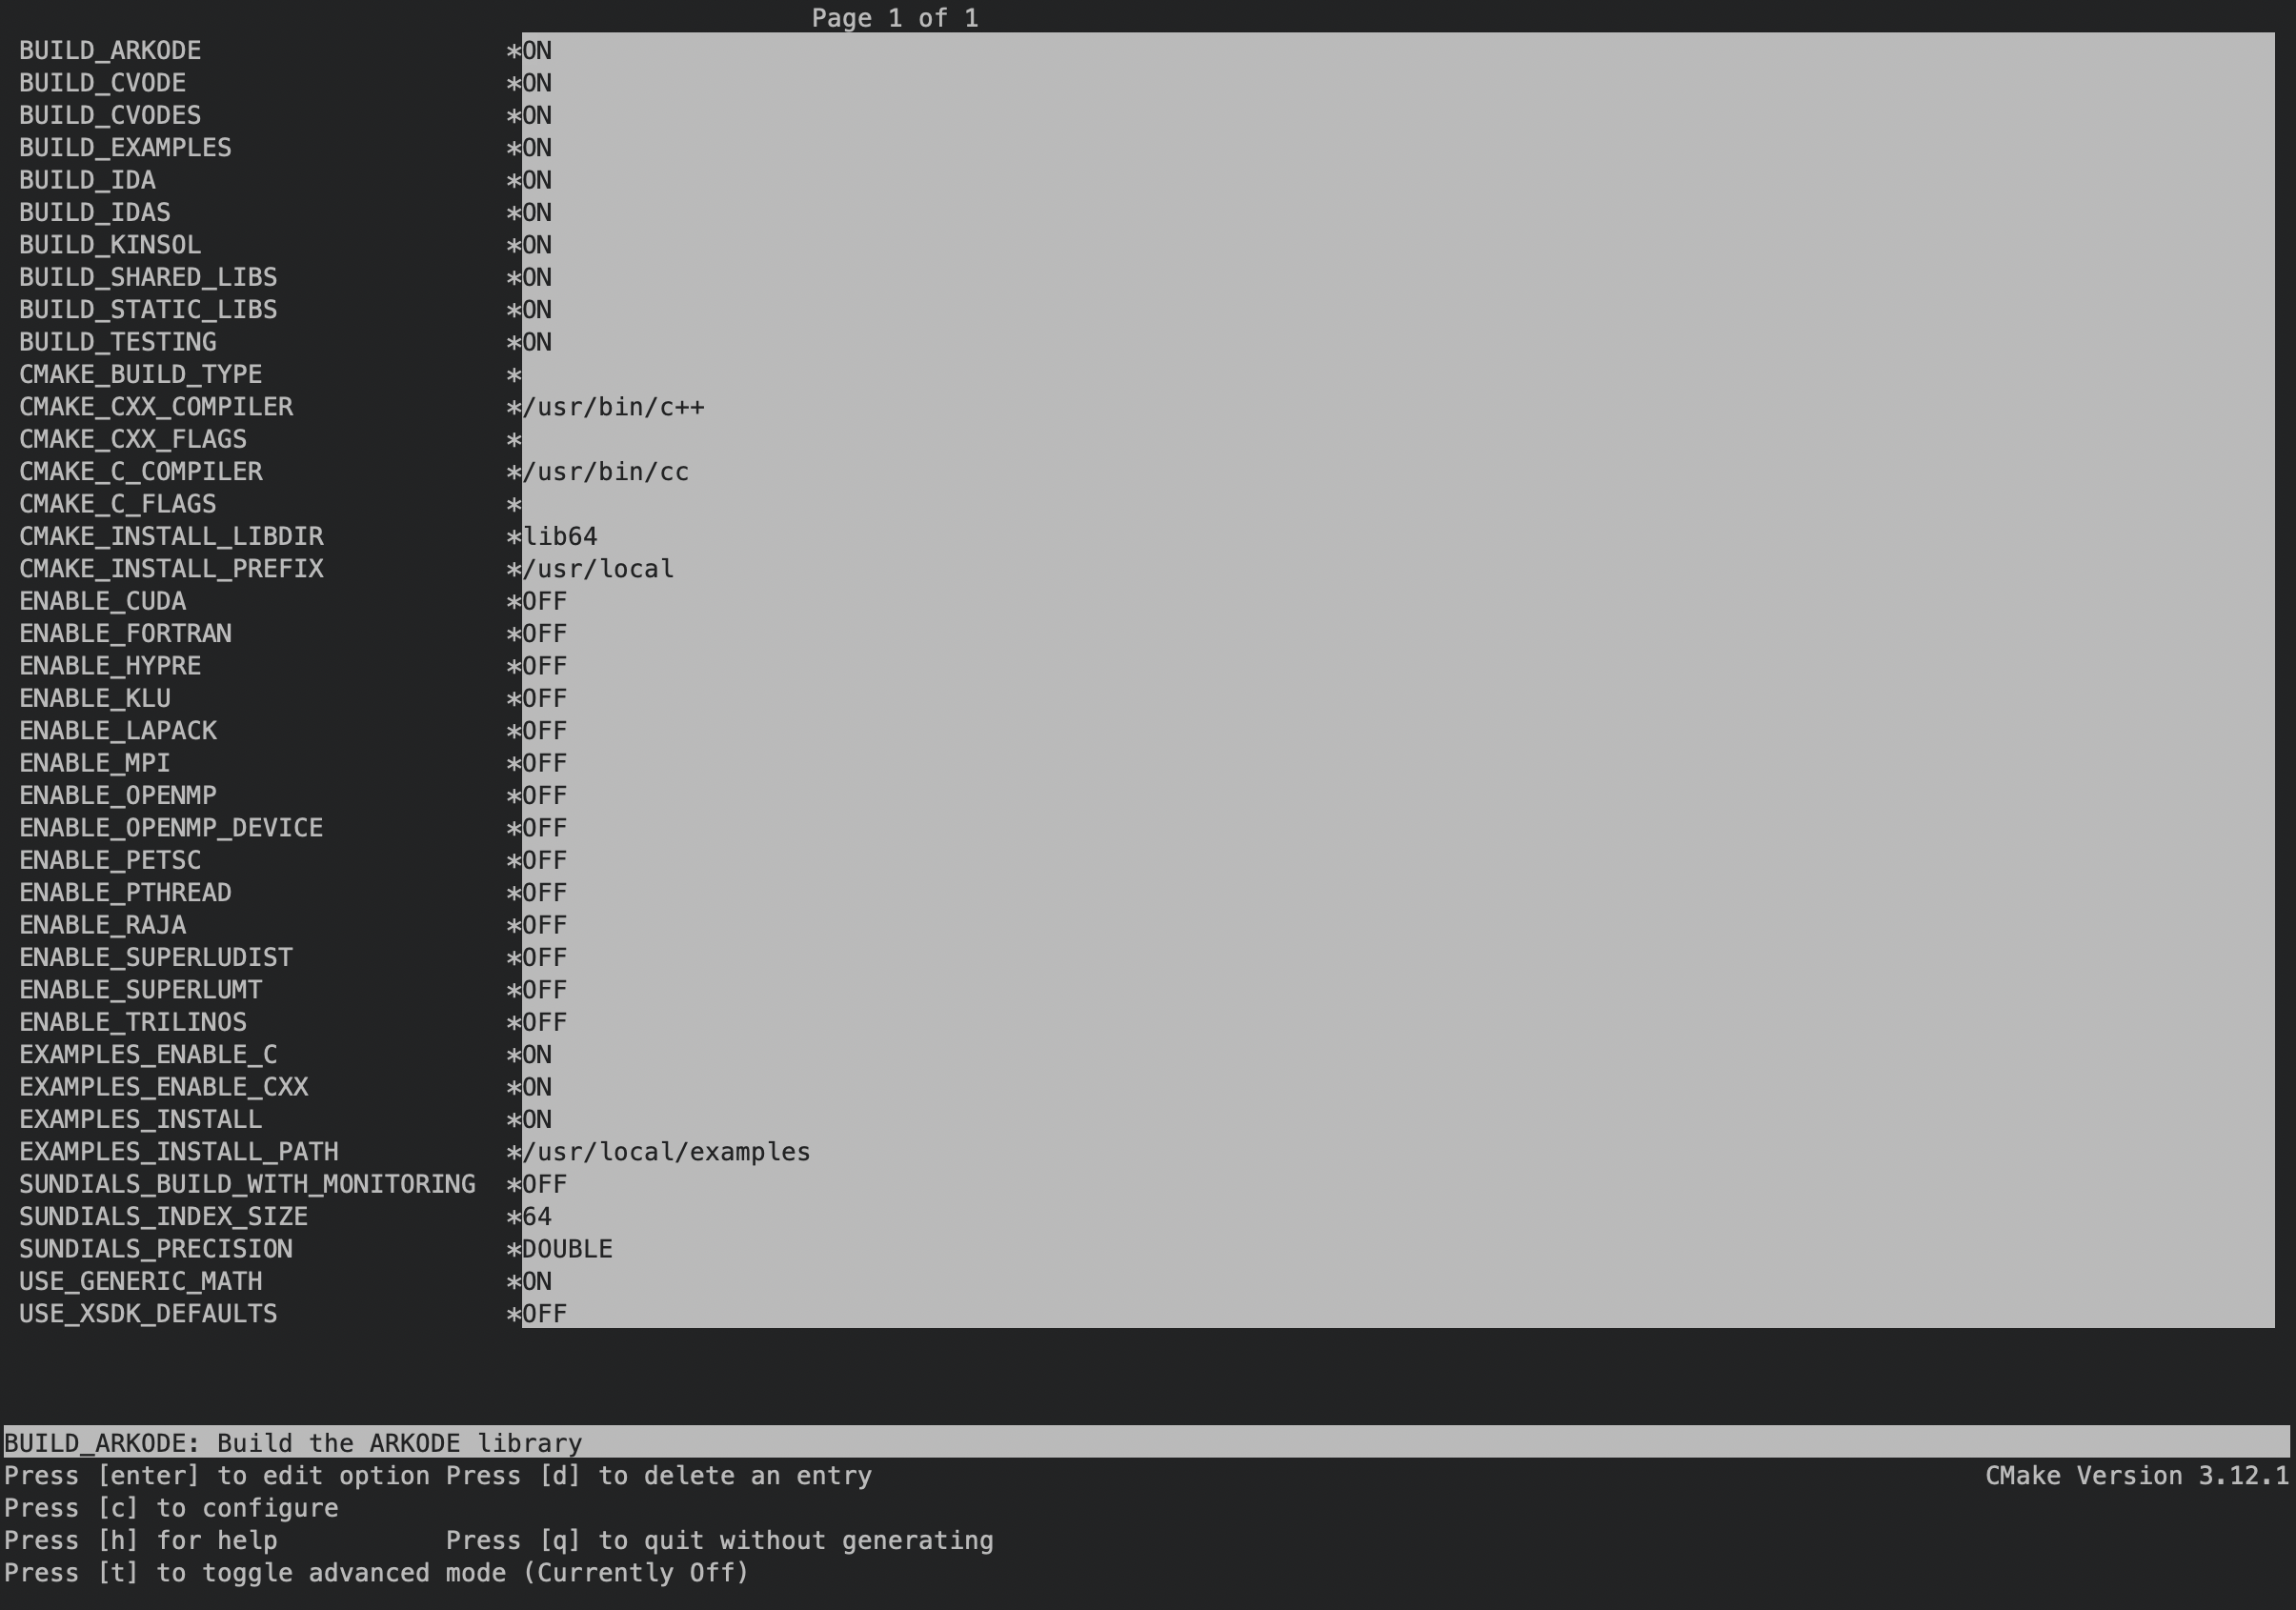
\includegraphics[width=\textwidth]{ccmakedefault}}}
\caption [Initial {\em ccmake} configuration screen]
{Default configuration screen. Note: Initial screen is empty.
To get this default configuration, press 'c' repeatedly (accepting default values denoted with asterisk)
until the 'g' option is available.}
\label{f:ccmakedefault}
\end{figure}

The default {\em instdir} for both {\sundials} and corresponding examples
can be changed by setting the \id{CMAKE\_INSTALL\_PREFIX} and
the \id{EXAMPLES\_INSTALL\_PATH} as shown in figure
\ref{f:ccmakeprefix}.
\begin{figure}[!ht]
{\centerline{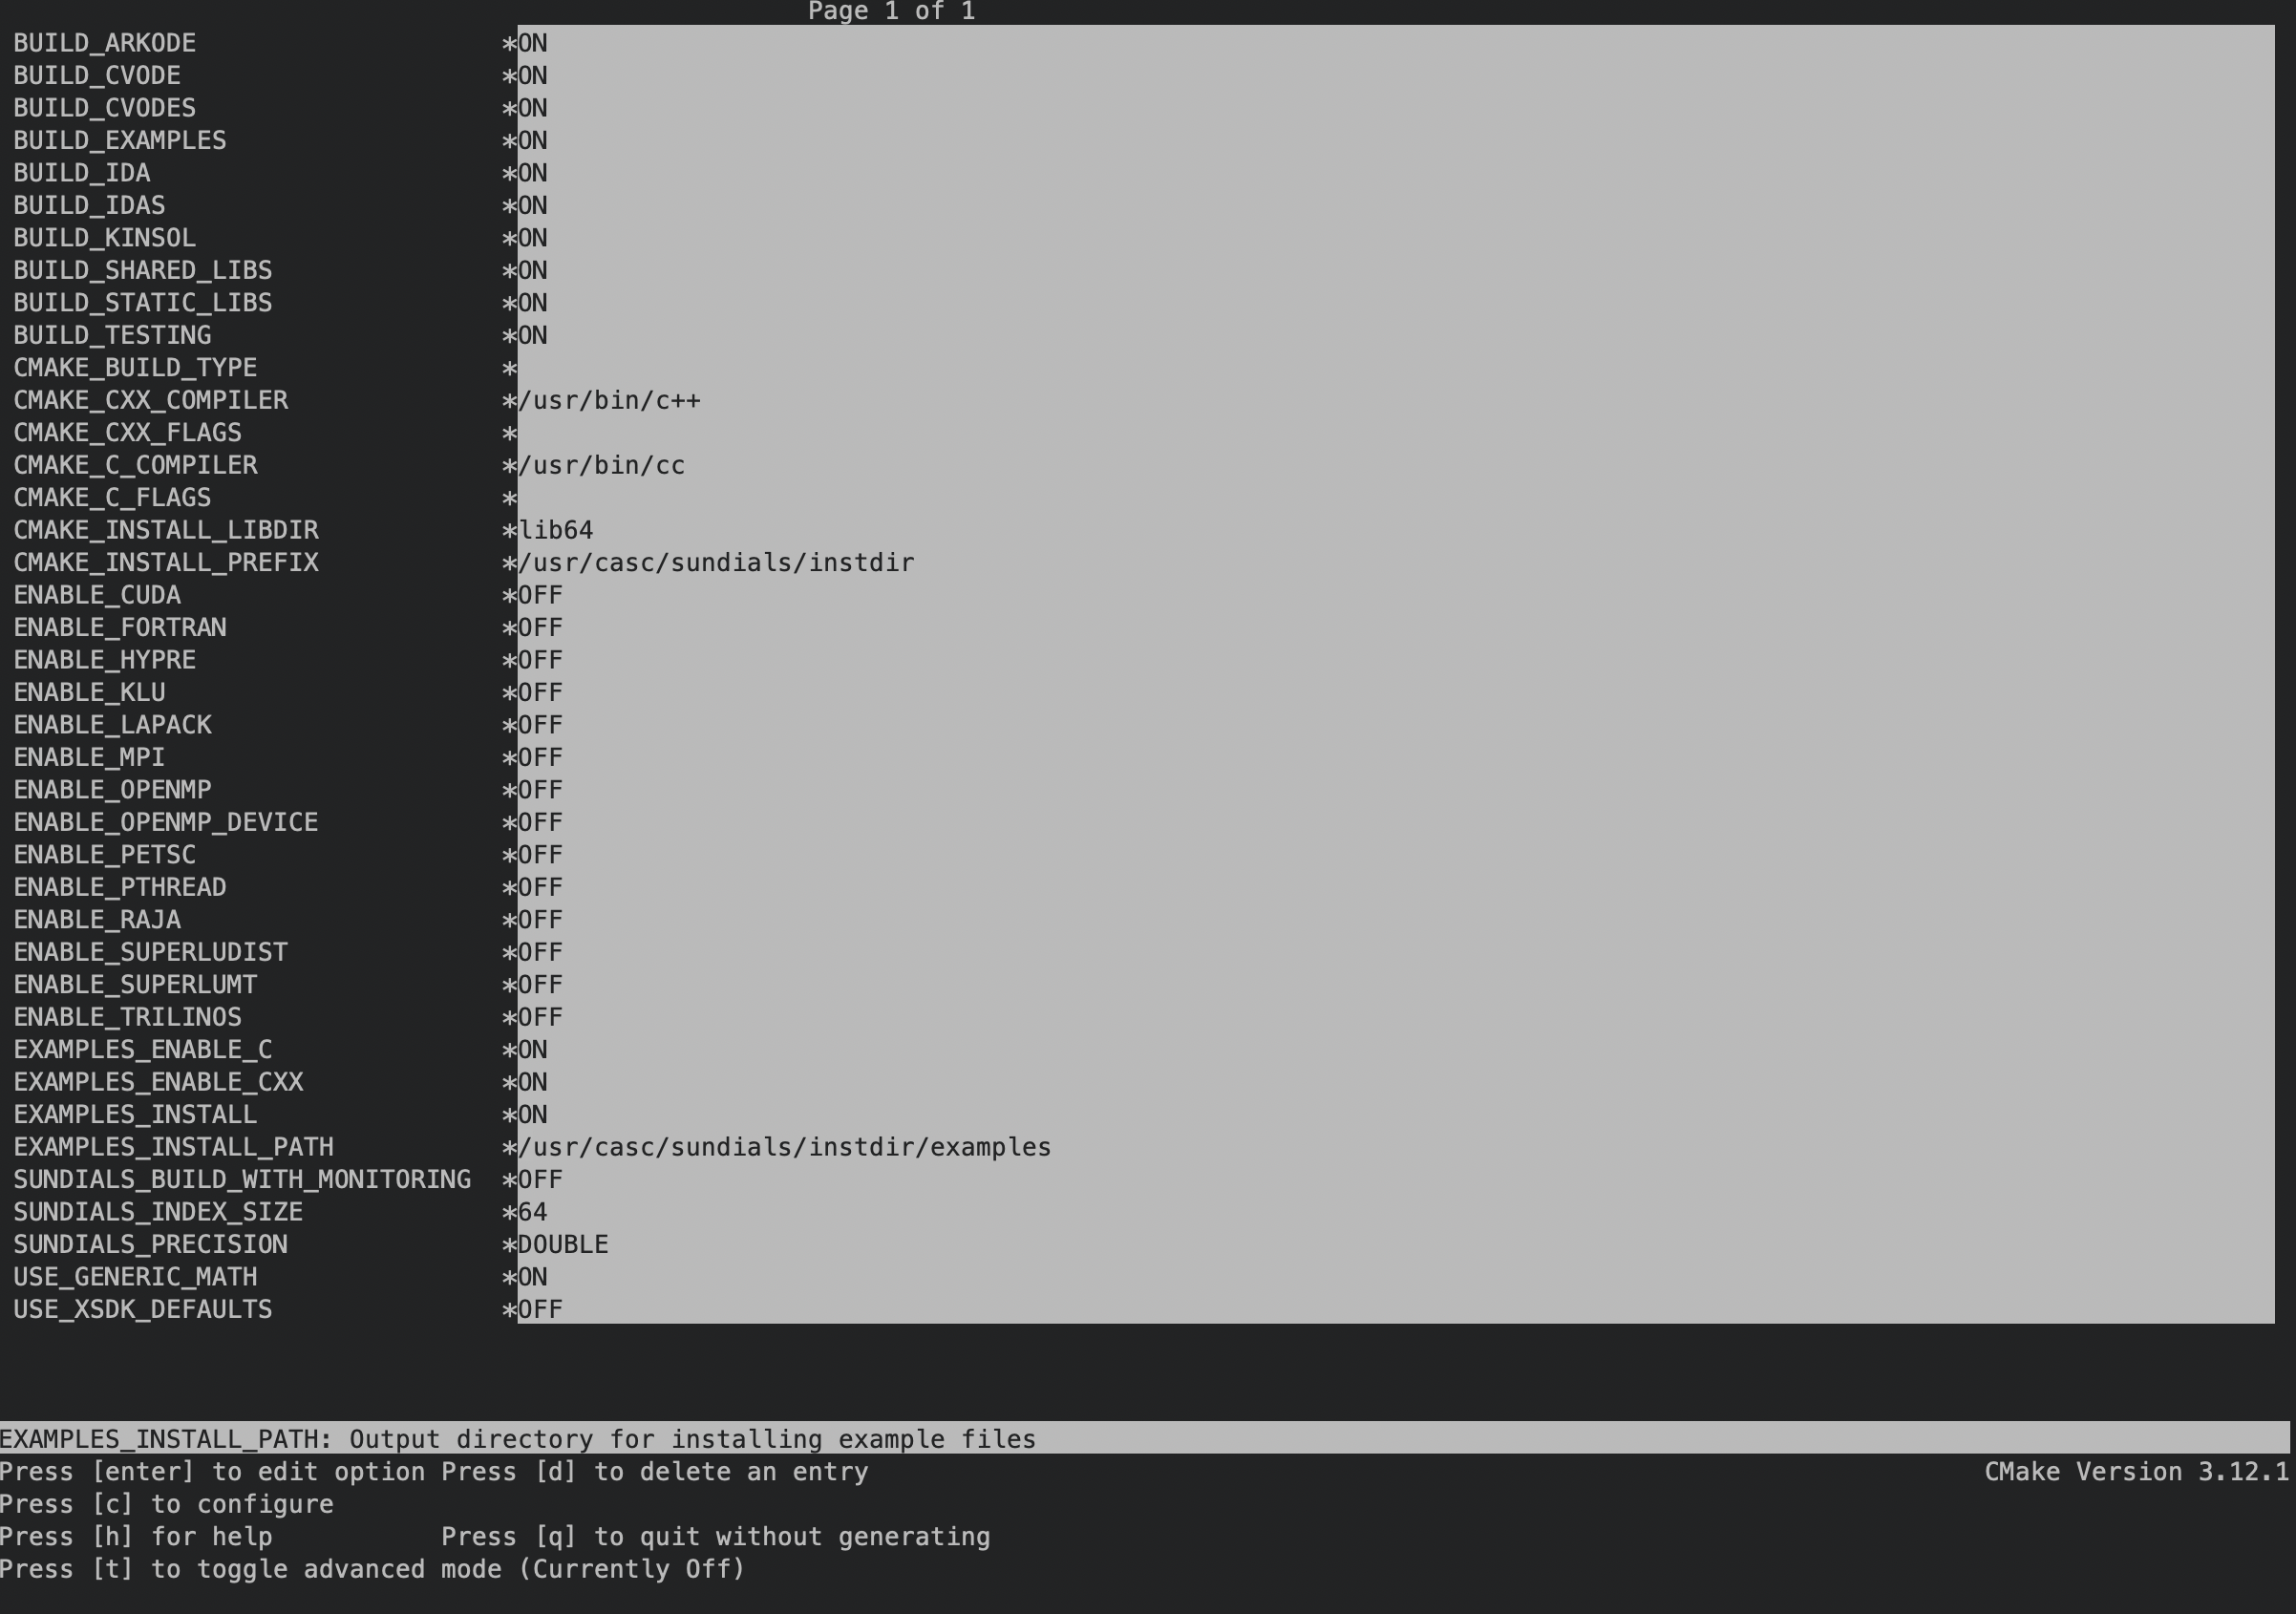
\includegraphics[width=\textwidth]{ccmakeprefix}}}
\caption [Changing the {\em instdir}]
{Changing the {\em instdir} for {\sundials} and
corresponding {\id examples} }
\label{f:ccmakeprefix}
\end{figure}

Pressing the (\id{g} key) will generate makefiles including all dependencies
and all rules to build {\sundials} on this system.
Back at the command prompt, you can now run:

\begin{verbatim}
  % make
\end{verbatim}

To install {\sundials} in the installation directory specified in the configuration, simply run:

\begin{verbatim}
  % make install
\end{verbatim}

%%
%% *** NOTE: The TestRunner will not be distributed at this time.
%% *** Thus the following is commented out from the documentation.
%% TestRunner
%%
%\subsubsection*{Testing Installation}
%The distribution of {\sundials} includes several examples corresponding to the solvers to be
%installed. Also included in the source bundle is a test script: \id{testRunner}, configured by CMake
%to test the included examples.
%To run the tests, enter:

%\begin{verbatim}
%  % make test
%\end{verbatim}
%The output of \id{testRunner} should look similar to the screens in figure
%\ref{f:testrunner}. The success of each test is based on a line-by-line comparison of expected output files, bundled with the source code, with
%the output of the newly compiled examples. The file compare does allow some differences in rounding for float values.\\\\
%NOTE: Some tests may {\em fail} due to differences in machine architecture, compiler versions, third party libraries etc.{\warn}

%\begin{figure}[!ht]
%{\centerline{\includegraphics{figure=testrunnertop.eps,width=\textwidth}}}
%\vspace{3 mm}
%{\centerline{\includegraphics{figure=testrunnerbot.eps,width=\textwidth}}}
%\caption [Running {\em testRunner}]
%{Invoking {\em testRunner} with {\id make test} to execute all configured
%{\id examples} }
%\label{f:testrunner}
%\end{figure}


%%
%% Building from the command line
%%
\subsubsection*{Building from the command line}

Using CMake from the command line is simply a matter of specifying CMake variable settings
with the \id{cmake} command.  The following will build the default configuration:

\begin{verbatim}
   % cmake -DCMAKE_INSTALL_PREFIX=/home/myname/sundials/instdir \
   > -DEXAMPLES_INSTALL_PATH=/home/myname/sundials/instdir/examples \
   > ../solverdir
   % make
   % make install
\end{verbatim}


\subsection{Configuration options (Unix/Linux)}\label{ss:configuration_options_nix}

A complete list of all available options for a CMake-based {\sundials}
configuration is provide below. Note that the default values shown are for
a typical configuration on a Linux system and are provided as illustration only.

\begin{description}
\item[\id{BUILD\_ARKODE}] -
  Build the ARKODE library
  \\
  Default: ON
\item[\id{BUILD\_CVODE}] -
  Build the CVODE library
  \\
  Default: ON
\item[\id{BUILD\_CVODES}] -
  Build the CVODES library
  \\
  Default: ON
\item[\id{BUILD\_IDA}] -
   Build the IDA library
  \\
   Default: ON
\item[\id{BUILD\_IDAS}] -
  Build the IDAS library
  \\
  Default: ON
\item[\id{BUILD\_KINSOL}] -
  Build the KINSOL library
  \\
  Default: ON
\item[\id{BUILD\_SHARED\_LIBS}] -
  Build shared libraries
  \\
  Default: ON
\item[\id{BUILD\_STATIC\_LIBS}] -
  Build static libraries
  \\
  Default: ON
\item[\id{CMAKE\_BUILD\_TYPE}] -
  Choose the type of build, options are:
  \id{None} (CMAKE\_C\_FLAGS used), \id{Debug}, \id{Release},
  \id{RelWithDebInfo}, and \id{MinSizeRel}
  \\
  Default:
  \\
  Note: Specifying a build type will trigger the corresponding
  build type specific compiler flag options below which will be
  appended to the flags set by
  CMAKE\_{\textless}language{\textgreater}\_FLAGS.
\item[\id{CMAKE\_C\_COMPILER}] -
  C compiler
  \\
  Default: /usr/bin/cc
\item[\id{CMAKE\_C\_FLAGS}] -
  Flags for C compiler
  \\
  Default:
\item[\id{CMAKE\_C\_FLAGS\_DEBUG}] -
  Flags used by the C compiler during debug builds
  \\
  Default: -g
\item[\id{CMAKE\_C\_FLAGS\_MINSIZEREL}] -
  Flags used by the C compiler during release minsize builds
  \\
  Default: -Os -DNDEBUG
\item[\id{CMAKE\_C\_FLAGS\_RELEASE}] -
  Flags used by the C compiler during release builds
  \\
  Default: -O3 -DNDEBUG
\item[\id{CMAKE\_CXX\_COMPILER}] -
  {\CPP} compiler
  \\
  Default: /usr/bin/c++
  \\
  Note: A {\CPP} compiler (and all related options) are only
  triggered if {\CPP} examples are enabled (\id{EXAMPLES\_ENABLE\_CXX}
  is ON). All {\sundials} solvers can be used from {\CPP} applications
  by default without setting any additional configuration options.
\item[\id{CMAKE\_CXX\_FLAGS}] -
  Flags for {\CPP} compiler
  \\
  Default:
\item[\id{CMAKE\_CXX\_FLAGS\_DEBUG}] -
  Flags used by the {\CPP} compiler during debug builds
  \\
  Default: -g
\item[\id{CMAKE\_CXX\_FLAGS\_MINSIZEREL}] -
  Flags used by the {\CPP} compiler during release minsize builds
  \\
  Default: -Os -DNDEBUG
\item[\id{CMAKE\_CXX\_FLAGS\_RELEASE}] -
  Flags used by the {\CPP} compiler during release builds
  \\
  Default: -O3 -DNDEBUG
\item[\id{CMAKE\_CXX\_STANDARD}] -
  The C++ standard to build C++ parts of {\sundials} with.
  \\
  Default: 11
  \\
  Note: Options are 98, 11, 14, 17, 20. This option is on used when a C++
  compiler is required.
\item[\id{CMAKE\_Fortran\_COMPILER}] -
  Fortran compiler
  \\
  Default: /usr/bin/gfortran
  \\
  Note: Fortran support (and all related options) are triggered only if
  either Fortran-C support is enabled (\id{FCMIX\_ENABLE} is ON) or
  LAPACK support is enabled (\id{ENABLE\_LAPACK} is ON).
\item[\id{CMAKE\_Fortran\_FLAGS}] -
  Flags for Fortran compiler
  \\
  Default:
\item[\id{CMAKE\_Fortran\_FLAGS\_DEBUG}] -
  Flags used by the Fortran compiler during debug builds
  \\
  Default: -g
\item[\id{CMAKE\_Fortran\_FLAGS\_MINSIZEREL}] -
  Flags used by the Fortran compiler during release minsize builds
  \\
  Default: -Os
\item[\id{CMAKE\_Fortran\_FLAGS\_RELEASE}] -
  Flags used by the Fortran compiler during release builds
  \\
  Default: -O3
\item[\id{CMAKE\_INSTALL\_PREFIX}] -
  Install path prefix, prepended onto install directories
  \\
  Default: /usr/local
  \\
  Note: The user must have write access to the location specified through
  this option. Exported {\sundials} header files and libraries will be
  installed under subdirectories \id{include} and
  \id{CMAKE\_INSTALL\_LIBDIR} of \id{CMAKE\_INSTALL\_PREFIX}, respectively.
\item[\id{CMAKE\_INSTALL\_LIBDIR}] -
  Library installation directory
  \\
  Default:
  \\
  Note: This is the directory within \id{CMAKE\_INSTALL\_PREFIX} that the {\sundials}
  libraries will be installed under. The default is automatically set based on the
  operating system using the GNUInstallDirs CMake module.
\item[\id{Fortran\_INSTALL\_MODDIR}] -
  Fortran module installation directory
  \\
  Default: fortran
\item[\id{ENABLE\_CUDA}] -
  Build the {\sundials} {\cuda} modules.
  \\
  Default: OFF
\item[\id{CUDA\_ARCH}] -
  Specifies the CUDA architecture to compile for.
  \\
  Default: sm\_30
\item[\id{EXAMPLES\_ENABLE\_C}] -
  Build the {\sundials} {\CC} examples
  \\
  Default: ON
\item[\id{EXAMPLES\_ENABLE\_CUDA}] -
  Build the {\sundials} {\cuda} examples
  \\
  Default: OFF
  \\
  Note: You need to enable {\cuda} support to build these examples.
\item[\id{EXAMPLES\_ENABLE\_CXX}] -
  Build the {\sundials} {\CPP} examples
  \\
  Default: OFF unless \id{ENABLE\_TRILINOS} is ON.
\item[\id{EXAMPLES\_ENABLE\_F77}] -
  Build the {\sundials} Fortran77 examples
  \\
  Default: ON (if \id{F77\_INTERFACE\_ENABLE} is ON)
\item[\id{EXAMPLES\_ENABLE\_F90}] -
  Build the {\sundials} Fortran90 examples
  \\
  Default: ON (if \id{F77\_INTERFACE\_ENABLE} is ON)
\item[\id{EXAMPLES\_ENABLE\_F2003}] -
  Build the {\sundials} Fortran2003 examples
  \\
  Default: ON (if \id{BUILD\_FORTRAN\_MODULE\_INTERFACE} is ON)
\item[\id{EXAMPLES\_INSTALL}] -
  Install example files
  \\
  Default: ON
  \\
  Note: This option is triggered when any of the {\sundials}
  example programs are enabled \\
  (\id{EXAMPLES\_ENABLE\_$<$language$>$} is ON). If the user requires
  installation of example programs then the sources and sample output files
  for all {\sundials} modules that are currently enabled will be exported to
  the directory specified by \id{EXAMPLES\_INSTALL\_PATH}. A CMake configuration
  script will also be automatically generated and exported to the same directory.
  Additionally, if the configuration is done under a Unix-like system, makefiles
  for the compilation of the example programs (using the installed {\sundials} libraries)
  will be automatically generated and exported to the directory
  specified by \id{EXAMPLES\_INSTALL\_PATH}.
\item[\id{EXAMPLES\_INSTALL\_PATH}] -
  Output directory for installing example files
  \\
  Default: /usr/local/examples
  \\
  Note: The actual default value for this option will be an \id{examples}
  subdirectory created under \id{CMAKE\_INSTALL\_PREFIX}.
\item[\id{F77\_INTERFACE\_ENABLE}] -
  Enable Fortran-C support via the Fortran 77 interfaces
  \\
  Default: OFF
\item[\id{BUILD\_FORTRAN\_MODULE\_INTERFACE}] -
  Enable Fortran-C support via the Fortran 2003 interfaces
  \\
  Default: OFF
\item[\id{ENABLE\_HYPRE}] -
  Enable {\hypre} support
  \\
  Default: OFF
  \\
  Note: See additional information on building with {\hypre} enabled in
  \ref{ss:externallibs}.
\item[\id{HYPRE\_INCLUDE\_DIR}] -
  Path to {\hypre} header files
\item[\id{HYPRE\_LIBRARY\_DIR}] -
  Path to {\hypre} installed library files
\item[\id{ENABLE\_KLU}] -
  Enable KLU support
  \\
  Default: OFF
  \\
  Note: See additional information on building with KLU enabled in
  \ref{ss:externallibs}.
\item[\id{KLU\_INCLUDE\_DIR}] -
  Path to SuiteSparse header files
\item[\id{KLU\_LIBRARY\_DIR}] -
  Path to SuiteSparse installed library files
\item[\id{ENABLE\_LAPACK}] -
  Enable LAPACK support
  \\
  Default: OFF
  \\
  Note: Setting this option to ON will trigger additional CMake
  options. See additional information on building with LAPACK enabled
  in \ref{ss:externallibs}.
\item[\id{LAPACK\_LIBRARIES}] -
  LAPACK (and BLAS) libraries
  \\
  Default: /usr/lib/liblapack.so;/usr/lib/libblas.so
  \\
  Note: CMake will search for libraries in your \id{LD\_LIBRARY\_PATH} prior
  to searching default system paths.
\item[\id{ENABLE\_MPI}] -
  Enable MPI support. This will build the parallel {\nvector} and the
  MPI-aware version of the ManyVector library.
  \\
  Default: OFF
  \\
  Note: Setting this option to ON will trigger several additional options
  related to MPI.
\item[\id{MPI\_C\_COMPILER}] -
  \id{mpicc} program
  \\
  Default:
\item[\id{MPI\_CXX\_COMPILER}] -
  \id{mpicxx} program
  \\
  Default:
  \\
  Note: This option is triggered only if MPI is enabled
  (\id{ENABLE\_MPI} is ON) and {\CPP} examples are enabled
  (\id{EXAMPLES\_ENABLE\_CXX} is ON). All {\sundials}
  solvers can be used from {\CPP} MPI applications by default
  without setting any additional configuration options other than
  \id{ENABLE\_MPI}.
\item[\id{MPI\_Fortran\_COMPILER}] -
  \id{mpif77} or \id{mpif90} program
  \\
  Default:
  \\
  Note: This option is triggered only if MPI is enabled
  (\id{ENABLE\_MPI} is ON) and Fortran-C support is enabled
  (\id{F77\_INTERFACE\_ENABLE} or \id{BUILD\_FORTRAN\_MODULE\_INTERFACE} is ON).
\item[\id{MPIEXEC\_EXECUTABLE}] -
  Specify the executable for running MPI programs
  \\
  Default: \id{mpirun}
  \\
  Note: This option is triggered only if MPI is enabled
  (\id{ENABLE\_MPI} is ON).
  %% \\
  %% Note: This can either be set to \id{mpirun} for OpenMPI or \id{srun} if jobs are
  %% managed by \id{SLURM} - Simple Linux Utility for Resource Management as exists on
  %% LLNL's high performance computing clusters.
\item[\id{ENABLE\_OPENMP}] -
  Enable {\openmp} support (build the {\openmp} {\nvector}).
  \\
  Default: OFF
\item[\id{OPENMP\_DEVICE\_ENABLE}] -
  Enable {\openmp} device offloading (build the OpenMPDEV nvector) if supported by
  the provided compiler.
  \\
  Default: OFF
\item[\id{OPENMP\_DEVICE\_WORKS}] - \textbf{advanced option} -
  Skip the check done to see if the {\openmp} provided by the compiler
  supports {\openmp} device offloading.
  \\
  Default: OFF
\item[\id{ENABLE\_PETSC}] -
  Enable {\petsc} support
  \\
  Default: OFF
  \\
  Note: See additional information on building with {\petsc} enabled
  in \ref{ss:build_with_petsc}.
\item[\id{PETSC\_DIR}] -
  Path to {\petsc} installation
  \\
  Default:
\item[\id{PETSC\_LIBRARIES}] - \textbf{advanced option} -
  Semi-colon separated list of PETSc link libraries. Unless provided by the
  user, this is autopopulated based on the PETSc installation found in
  \id{PETSC\_DIR}.
  \\
  Default:
\item[\id{PETSC\_INCLUDES}] - \textbf{advanced option} -
  Semi-colon separated list of PETSc include directories. Unless provided by the
  user, this is autopopulated based on the PETSc installation found in
  \id{PETSC\_DIR}.
  \\
  Default:
\item[\id{ENABLE\_PTHREAD}] -
  Enable Pthreads support (build the Pthreads {\nvector}).
  \\
  Default: OFF
\item[\id{ENABLE\_RAJA}] -
  Enable {\raja} support.
  \\
  Default: OFF
  \\
  Note: You need to enable CUDA or HIP in order to build the {\raja} vector module.
\item[\id{SUNDIALS\_RAJA\_BACKENDS}] -
  If building SUNDIALS with RAJA support, this sets the RAJA
  backend to target. Values supported are CUDA and HIP.
  \\
  Default: CUDA
\item[\id{ENABLE\_SUPERLUDIST}] -
  Enable {\superludist} support
  \\
  Default: OFF
  \\
  Note: See additional information on building with {\superludist} enabled
  in \ref{ss:externallibs}.
\item[\id{SUPERLUDIST\_INCLUDE\_DIR}] -
  Path to {\superludist} header files (typically SRC directory)
\item[\id{SUPERLUDIST\_LIBRARY\_DIR}] -
  Path to {\superludist} installed library files
\item[\id{SUPERLUDIST\_LIBRARIES}] -
  Semi-colon separated list of libraries needed for {\superludist}
\item[\id{SUPERLUDIST\_OpenMP}] -
  Enable {\sundials} support for {\superludist} built with {\openmp}
  \\
  Default: OFF
  \\
  Note: {\superludist} must be built with {\openmp} support for this option to function
  properly. Additionally the environment variable \id{OMP\_NUM\_THREADS} must be set to
  the desired number of threads.
\item[\id{ENABLE\_SUPERLUMT}] -
  Enable {\superlumt} support
  \\
  Default: OFF
  \\
  Note: See additional information on building with {\superlumt} enabled
  in \ref{ss:externallibs}.
\item[\id{SUPERLUMT\_INCLUDE\_DIR}] -
  Path to SuperLU\_MT header files (typically SRC directory)
\item[\id{SUPERLUMT\_LIBRARY\_DIR}] -
  Path to SuperLU\_MT installed library files
\item[\id{SUPERLUMT\_LIBRARIES}] -
  Semi-colon separated list of libraries needed for SuperLU\_MT
\item[\id{SUPERLUMT\_THREAD\_TYPE}] -
  Must be set to Pthread or {\openmp}
  \\
  Default: Pthread
\item[\id{ENABLE\_SYCL}] -
  Enable {\sycl} support.
  \\
  Default: OFF
  \\
  Note: At present the only supported SYCL compiler is the DPC++ (Intel oneAPI)
  compiler. CMake does not currently support autodetection of SYCL compilers and
  \id{CMAKE\_CXX\_COMPILER} must be set to a valid SYCL compiler i.e.,
  \id{dpcpp} in order to build with SYCL support.
\item[\id{ENABLE\_TRILINOS}] -
  Enable {\trilinos} support (build the {\tpetra} {\nvector}).
  \\
  Default: OFF
\item[\id{Trilinos\_DIR}] -
  Path to the Trilinos install directory.
  \\
  Default:
\item[\id{TRILINOS\_INTERFACE\_C\_COMPILER}] - \textbf{advanced option} -
  Set the {\CC} compiler for building the {\trilinos} interface
  (i.e., {\nvectrilinos} and the examples that use it).
  \\
  Default: The {\CC} compiler exported from the found {\trilinos} installation
  if \id{USE\_XSDK\_DEFAULTS=OFF}. \id{CMAKE\_C\_COMPILER} or \id{MPI\_C\_COMPILER} if \id{USE\_XSDK\_DEFAULTS=ON}.
  \\
  Note: It is recommended to use the same compiler that was used to build the {\trilinos} library.
\item[\id{TRILINOS\_INTERFACE\_C\_COMPILER\_FLAGS}] - \textbf{advanced option} -
  Set the {\CC} compiler flags for {\trilinos} interface
  (i.e., {\nvectrilinos} and the examples that use it).
  \\
  Default: The {\CC} compiler flags exported from the found {\trilinos} installation
  if \id{USE\_XSDK\_DEFAULTS=OFF}. \id{CMAKE\_C\_FLAGS} if \id{USE\_XSDK\_DEFAULTS=ON}.
  \\
  Note: It is recommended to use the same flags that were used to build the {\trilinos} library.
\item[\id{TRILINOS\_INTERFACE\_CXX\_COMPILER}] - \textbf{advanced option} -
  Set the {\CPP} compiler for builing {\trilinos} interface
  (i.e., {\nvectrilinos} and the examples that use it).
  \\
  Default: The {\CPP} compiler exported from the found {\trilinos} installation
  if \id{USE\_XSDK\_DEFAULTS=OFF}. \id{CMAKE\_CXX\_COMPILER} or \id{MPI\_CXX\_COMPILER} if \id{USE\_XSDK\_DEFAULTS=ON}.
  \\
  Note: It is recommended to use the same compiler that was used to build the {\trilinos} library.
\item[\id{TRILINOS\_INTERFACE\_CXX\_COMPILER\_FLAGS}] - \textbf{advanced option} -
  Set the {\CPP} compiler flags for {\trilinos} interface
  (i.e., {\nvectrilinos} and the examples that use it).
  \\
  Default: The {\CPP} compiler flags exported from the found {\trilinos} installation
  if \id{USE\_XSDK\_DEFAULTS=OFF}. \id{CMAKE\_CXX\_FLAGS} if \id{USE\_XSDK\_DEFAULTS=ON}.
  \\
  Note: Is is recommended to use the same flags that were used to build the {\trilinos} library.
\item[\id{SUNDIALS\_BUILD\_WITH\_MONITORING}] -
  Build {\sundials} with capabilties for fine-grained monitoring of solver progress
  and statistics. This is primarily useful for debugging.
  \\
  Default: OFF
  \\
  Note: Building with monitoring may result in minor performance degradation
  even if monitoring is not utilized.
\item[\id{SUNDIALS\_BUILD\_PACKAGE\_FUSED\_KERNELS}] -
  Build specialized fused kernels inside {\cvode}.
  \\
  Default: OFF
  \\
  Note: This option is currently only available when building with
  \id{CUDA\_ENABLE = ON}. Building with fused kernels requires
  linking to either \id{libsundials\_cvode\_fused\_cuda.{\em lib}} or
  \id{libsundials\_cvode\_fused\_stubs.{\em lib}}, where the latter
  provides CPU-only placeholders for the fused routines, in
  addition to \id{libsundials\_cvode.{\em lib}}.
\item[\id{CMAKE\_CXX\_STANDARD}] -
  The C++ standard to build C++ parts of {\sundials} with.
  \\
  Default: 11
  \\
  Note: Options are 99, 11, 14, 17. This option only used when a
  C++ compiler is required.
\item[\id{SUNDIALS\_F77\_FUNC\_CASE}] - \textbf{advanced option} -
  Specify the case to use in the Fortran name-mangling scheme, options
  are: \id{lower} or \id{upper}
  \\
  Default:
  \\
  Note: The build system will attempt to infer the Fortran
  name-mangling scheme using the Fortran compiler. This option should
  only be used if a Fortran compiler is not available or to override
  the inferred or default (\id{lower}) scheme if one can not be
  determined. If used, \id{SUNDIALS\_F77\_FUNC\_UNDERSCORES} must also
  be set.
\item[\id{SUNDIALS\_F77\_FUNC\_UNDERSCORES}] - \textbf{advanced option} -
  Specify the number of underscores to append in the Fortran
  name-mangling scheme, options are: \id{none}, \id{one}, or \id{two}
  \\
  Default:
  \\
  Note: The build system will attempt to infer the Fortran
  name-mangling scheme using the Fortran compiler. This option should
  only be used if a Fortran compiler is not available or to override
  the inferred or default (\id{one}) scheme if one can not be
  determined. If used, \id{SUNDIALS\_F77\_FUNC\_CASE} must also be set.
\item[\id{SUNDIALS\_INDEX\_TYPE}] - \textbf{advanced option} -
  Integer type used for {\sundials} indices. The size must match the size provided for
  the \\ \noindent \id{SUNDIALS\_INDEX\_SIZE} option.
  \\
  Default:
  \\
  Note:
  In past SUNDIALS versions, a user could set this option to \id{INT64\_T} to use 64-bit
  integers, or \id{INT32\_T} to use 32-bit integers. Starting in SUNDIALS 3.2.0, these
  special values are deprecated. For SUNDIALS 3.2.0 and up, a user will only need to use
  the \id{SUNDIALS\_INDEX\_SIZE} option in most cases.
\item[\id{SUNDIALS\_INDEX\_SIZE}] -
  Integer size (in bits) used for indices in {\sundials}, options are: \id{32} or \id{64}
  \\
  Default: \id{64}
  \\
  Note:
  The build system tries to find an integer type of appropriate size. Candidate 64-bit
  integer types are (in order of preference): \id{int64\_t}, \id{\_\_int64}, \id{long long}, and \id{long}.
  Candidate 32-bit integers are (in order of preference): \id{int32\_t}, \id{int}, and \id{long}.
  The advanced option, \id{SUNDIALS\_INDEX\_TYPE} can be used to provide a type not listed here.
\item[\id{SUNDIALS\_PRECISION}] -
  Precision used in {\sundials}, options are: \id{double}, \id{single}, or \id{extended}
  \\
  Default: \id{double}
\item[\id{SUNDIALS\_INSTALL\_CMAKEDIR}] -
  Installation directory for the {\sundials} cmake files (relative to \id{CMAKE\_INSTALL\_PREFIX}).
  \\
  Default: \id{CMAKE\_INSTALL\_PREFIX/cmake/sundials}
\item[\id{USE\_GENERIC\_MATH}] -
  Use generic (stdc) math libraries
  \\
  Default: ON
\item[\id{USE\_XSDK\_DEFAULTS}] -
  Enable xSDK (see \href{https://xsdk.info} for more information) default
  configuration settings. This sets \id{CMAKE\_BUILD\_TYPE} to \id{Debug},
  \id{SUNDIALS\_INDEX\_SIZE} to 32 and \id{SUNDIALS\_PRECISION} to double.
  \\
  Default: OFF
\end{description}



%%===============================================================================

\subsection{Configuration examples}

The following examples will help demonstrate usage of the CMake configure options.

\noindent To configure {\sundials} using the default C and Fortran compilers,
and default \id{mpicc} and \id{mpif77} parallel compilers,
enable compilation of examples, and install libraries, headers, and
example sources under subdirectories of
\id{/home/myname/sundials/}, use:

\begin{verbatim}
   % cmake \
   > -DCMAKE_INSTALL_PREFIX=/home/myname/sundials/instdir \
   > -DEXAMPLES_INSTALL_PATH=/home/myname/sundials/instdir/examples \
   > -DENABLE_MPI=ON \
   > -DFCMIX_ENABLE=ON \
   > /home/myname/sundials/solverdir
   %
   % make install
   %
\end{verbatim}

\noindent To disable installation of the examples, use:
\begin{verbatim}
   % cmake \
   > -DCMAKE_INSTALL_PREFIX=/home/myname/sundials/instdir \
   > -DEXAMPLES_INSTALL_PATH=/home/myname/sundials/instdir/examples \
   > -DENABLE_MPI=ON \
   > -DFCMIX_ENABLE=ON \
   > -DEXAMPLES_INSTALL=OFF \
   > /home/myname/sundials/solverdir
   %
   % make install
   %
\end{verbatim}

%%===============================================================================
\subsection{Working with external Libraries} \label{ss:externallibs}

The {\sundials} suite contains many options to enable implementation flexibility
when developing solutions. The following are some notes addressing specific configurations
when using the supported third party libraries.
When building {\sundials} as a shared library any external libraries
used with {\sundials} must also be build as a shared library or as a
static library compiled with the \id{-fPIC} flag.{\warn}

\subsubsection*{Building with LAPACK}
To enable LAPACK, set the \id{ENABLE\_LAPACK} option to \id{ON}.
If the directory containing the LAPACK library is in the
\id{LD\_LIBRARY\_PATH} environment variable, CMake will set the
\id{LAPACK\_LIBRARIES} variable accordingly, otherwise CMake will
attempt to find the LAPACK library in standard system locations. To
explicitly tell CMake what library to use, the \id{LAPACK\_LIBRARIES}
variable can be set to the desired libraries rquired for LAPACK.
\begin{verbatim}
   % cmake \
   > -DCMAKE_INSTALL_PREFIX=/home/myname/sundials/instdir \
   > -DEXAMPLES_INSTALL_PATH=/home/myname/sundials/instdir/examples \
   > -DENABLE_LAPACK=ON \
   > -DLAPACK_LIBRARIES=/mylapackpath/lib/libblas.so;/mylapackpath/lib/liblapack.so \
   > /home/myname/sundials/solverdir
   %
   % make install
   %
\end{verbatim}

If a working Fortran compiler is not available to infer the Fortran
name-mangling scheme, the options \id{SUNDIALS\_F77\_FUNC\_CASE} and
\id{SUNDIALS\_F77\_FUNC\_UNDERSCORES} \textit{must} be set in order to
bypass the check for a Fortran compiler and define the name-mangling
scheme. The defaults for these options in earlier versions of
{\sundials} were \id{lower} and \id{one} respectively.

\subsubsection*{Building with KLU}
The KLU libraries are part of SuiteSparse, a suite of sparse matrix software,
available from the Texas A\&M University website: {\tt
http://faculty.cse.tamu.edu/davis/suitesparse.html}.  {\sundials} has been
tested with SuiteSparse version 5.7.2.  To enable KLU, set \id{ENABLE\_KLU} to
\id{ON}, set \id{KLU\_INCLUDE\_DIR} to the \id{include} path of the KLU
installation and set \id{KLU\_LIBRARY\_DIR} to the \id{lib} path of the KLU
installation.  The CMake configure will result in populating the following
variables: \id{AMD\_LIBRARY}, \id{AMD\_LIBRARY\_DIR}, \id{BTF\_LIBRARY},
\id{BTF\_LIBRARY\_DIR}, \id{COLAMD\_LIBRARY}, \id{COLAMD\_LIBRARY\_DIR}, and
\newline\id{KLU\_LIBRARY}.

\subsubsection*{Building with SuperLU\_MT}
The SuperLU\_MT libraries are available for download from the Lawrence Berkeley
National Laboratory website: {\tt
http://crd-legacy.lbl.gov/$\sim$xiaoye/SuperLU/\#superlu\_mt}.  {\sundials} has
been tested with SuperLU\_MT version 3.1.  To enable SuperLU\_MT, set
\id{ENABLE\_SUPERLUMT} to \id{ON}, set \id{SUPERLUMT\_INCLUDE\_DIR} to the
\id{SRC} path of the SuperLU\_MT installation, and set the variable
\newline\id{SUPERLUMT\_LIBRARY\_DIR} to the \id{lib} path of the SuperLU\_MT
installation.  At the same time, the variable \id{SUPERLUMT\_LIBRARIES} must be
set to a semi-colon separated list of other libraries SuperLU\_MT depends on.
For example, if SuperLU\_MT ws build with an external blas library, then include
the full path to the blas library in this list. Additionally, the variable
\id{SUPERLUMT\_THREAD\_TYPE} must be set to either \id{Pthread} or
\id{{\openmp}}.

\noindent Do not mix thread types when building {\sundials} solvers.  If
threading is enabled for {\sundials} by having either \id{ENABLE\_OPENMP} or
\id{ENABLE\_PTHREAD} set to \id{ON} then SuperLU\_MT should be set to use the
same threading type.{\warn}

\subsubsection*{Building with {\superludist}}
The {\superludist} libraries are available for download from the Lawrence
Berkeley National Laboratory website: {\tt
http://crd-legacy.lbl.gov/$\sim$xiaoye/SuperLU/\#superlu\_dist}.  {\sundials}
has been tested with {\superludist} 6.1.1.  To enable {\superludist}, set
\id{ENABLE\_SUPERLUDIST} to \id{ON}, set \id{SUPERLUDIST\_INCLUDE\_DIR} to the
include directory of the {\superludist} installation (typically \id{SRC}), and
set the variable \newline\id{SUPERLUDIST\_LIBRARY\_DIR} to the path to library
directory of the {\superludist} installation (typically \id{lib}). At the same
time, the variable \id{SUPERLUDIST\_LIBRARIES} must be set to a semi-colon
separated list of other libraries {\superludist} depends on. For example, if
{\superludist} was built with LAPACK, then include the LAPACK library in this
list.  If {\superludist} was built with {\openmp} support, then you may set
\id{SUPERLUDIST\_OPENMP} to \id{ON} to utilize the {\openmp} functionality of
{\superludist}.

\noindent Do not mix thread types when building {\sundials} solvers.  If
threading is enabled for {\sundials} by having \id{ENABLE\_PTHREAD} set to
\id{ON} then {\superludist} should not be set to use {\openmp}.{\warn}

\subsubsection*{Building with PETSc}
\label{ss:building_with_petsc}
The {\petsc} libraries are available for download from the Argonne National
Laboratory website: {\tt http://www.mcs.anl.gov/petsc}. {\sundials} has been
tested with {\petsc} version 3.10.0--3.14.0. To enable {\petsc}, set
\id{ENABLE\_PETSC} to \id{ON} and then set \id{PETSC\_DIR} to the path of the
{\petsc} installation. Alternatively, a user can provide a list of include paths
in \id{PETSC\_INCLUDES}, and a list of complete paths to the libraries needed in
\id{PETSC\_LIBRARIES}.


\subsubsection*{Building with {\hypre}}
The {\hypre} libraries are available for download from the Lawrence Livermore
National Laboratory website: {\tt http://computing.llnl.gov/projects/hypre}.
{\sundials} has been tested with {\hypre} version 2.14.0--2.19.0.  To enable
{\hypre}, set  \id{ENABLE\_HYPRE} to \id{ON}, set \id{HYPRE\_INCLUDE\_DIR} to
the \id{include} path of the {\hypre} installation, and set the variable
\id{HYPRE\_LIBRARY\_DIR} to the \id{lib} path of the {\hypre} installation.

Note: {\sundials} must be configured so that \id{SUNDIALS\_INDEX\_SIZE} (or
equivalently, \id{XSDK\_INDEX\_SIZE}) equals the precision of
\id{HYPRE\_BigInt} in the corresponding {\hypre} installation.


\subsubsection*{Building with CUDA}
{\sundials} {\cuda} modules and examples have been tested with versions 9
through 11.0.2 of the {\cuda} toolkit. To build them, you need to install the
Toolkit and compatible NVIDIA drivers. Both are available for download from the
NVIDIA website: {\tt https://developer.nvidia.com/cuda-downloads}. To enable
{\cuda}, set \id{ENABLE\_CUDA} to \id{ON}. If {\cuda} is installed in a
nonstandard location, you may be prompted to set the variable
\id{CUDA\_TOOLKIT\_ROOT\_DIR} with your {\cuda} Toolkit installation path. To
enable {\cuda} examples, set \id{EXAMPLES\_ENABLE\_CUDA} to \id{ON}.

\subsubsection*{Building with RAJA}
{\raja} is a performance portability layer developed by Lawrence Livermore
National Laboratory and can be obtained from {\tt https://github.com/LLNL/RAJA}.
{\sundials} {\raja} modules and examples have been tested with {\raja} up to
version 0.12.1. Building {\sundials} {\raja} modules requires a {\cuda}-enabled
{\raja} installation. To enable {\raja}, set \id{ENABLE\_CUDA} and
\id{ENABLE\_RAJA} to \id{ON}. If {\raja} is installed in a nonstandard location
you will be prompted to set the variable \id{RAJA\_DIR} with the path to the
{\raja} CMake configuration file. To enable building the {\raja} examples set
\id{EXAMPLES\_ENABLE\_CUDA} to \id{ON}.

\subsubsection*{Building with Trilinos}
{\trilinos} is a suite of numerical libraries developed by Sandia National
Laboratories. It can be obtained at {\tt https://github.com/trilinos/Trilinos}.
{\sundials} {\trilinos} modules and examples have been tested with {\trilinos}
version 12.14.1 -- 12.18.1. To enable {\trilinos}, set
\id{ENABLE\_TRILINOS} to \id{ON}. If {\trilinos} is
installed in a nonstandard location you will be prompted to set the
variable \id{Trilinos\_DIR} with the path to the {\trilinos} CMake
configuration file. It is desireable to build the {\trilinos} vector interface
with same compiler and options that were used to build {\trilinos}.
CMake will try to find the correct compiler settings automatically from the
{\trilinos} configuration file. If that is not successful,
the compilers and options can be manually set with the following CMake variables:
\begin{itemize}
\item
\id{Trilinos\_INTERFACE\_C\_COMPILER}
\item
\id{Trilinos\_INTERFACE\_C\_COMPILER\_FLAGS}
\item
\id{Trilinos\_INTERFACE\_CXX\_COMPILER}
\item
\id{Trilinos\_INTERFACE\_CXX\_COMPILER\_FLAGS}
\end{itemize}

\subsection{Testing the build and installation}

If {\sundials} was configured with
\id{EXAMPLES\_ENABLE\_$<$language$>$} options to \id{ON}, then a set of
regression tests can be run after building with the \id{make} command
by running:
\begin{verbatim}
  % make test
\end{verbatim}
Additionally, if \id{EXAMPLES\_INSTALL} was also set to \id{ON}, then
a set of smoke tests can be run after installing with the \id{make install}
command by running:
\begin{verbatim}
  % make test_install
\end{verbatim}

%%===============================================================================
\section{Building and Running Examples}
%%===============================================================================
Each of the {\sundials} solvers is distributed with a set of examples
demonstrating basic usage. To build and install the examples, set at least of
the \id{EXAMPLES\_ENABLE\_$<$language$>$} options to \id{ON}, and set
\id{EXAMPLES\_INSTALL} to \id{ON}.  Specify the installation path for the
examples with the variable \id{EXAMPLES\_INSTALL\_PATH}. CMake will generate
\id{CMakeLists.txt} configuration files (and \id{Makefile} files if on
Linux/Unix) that reference the {\em installed} {\sundials} headers and
libraries.

Either the \id{CMakeLists.txt} file or the traditional \id{Makefile} may be used
to build the examples as well as serve as a template for creating user developed
solutions.  To use the supplied \id{Makefile} simply run \id{make} to compile
and generate the executables.  To use CMake from within the installed example
directory, run \id{cmake} (or \id{ccmake} to use the GUI) followed by \id{make}
to compile the example code.  Note that if CMake is used, it will overwrite the
traditional \id{Makefile} with a new CMake-generated \id{Makefile}.  The
resulting output from running the examples can be compared with example output
bundled in the {\sundials} distribution.

\noindent NOTE: There will potentially be differences in the output due to
machine architecture, compiler versions, use of third party libraries
etc.{\warn}


%%===============================================================================
\section{Configuring, building, and installing  on Windows}\label{s:cmake_windows}
%%===============================================================================
CMake can also be used to build {\sundials} on Windows. To build {\sundials} for
use with Visual Studio the following steps should be performed:
\begin{enumerate}
\item Unzip the downloaded tar file(s) into a directory. This will be the {\em solverdir}
\item Create a separate {\em builddir}
\item Open a Visual Studio Command Prompt and cd to {\em builddir}
\item Run cmake-gui ../{\em solverdir}
\begin{enumerate}
\item Hit Configure
\item Check/Uncheck solvers to be built
\item Change CMAKE\_INSTALL\_PREFIX to {\em instdir}
\item Set other options as desired
\item Hit Generate
\end{enumerate}
\item Back in the VS Command Window:
\begin{enumerate}
\item Run msbuild ALL\_BUILD.vcxproj
\item Run msbuild INSTALL.vcxproj
\end{enumerate}
\end{enumerate}

\noindent The resulting libraries will be in the {\em instdir}.
\noindent The {\sundials} project can also now be opened in Visual Studio.
Double click on the ALL\_BUILD.vcxproj file to open the project.
Build the whole {\em solution} to create the {\sundials} libraries.
To use the {\sundials} libraries in your own projects, you must
set the include directories for your project,
add the {\sundials} libraries to your project solution,
and set the {\sundials} libraries as dependencies for your project.

%%===============================================================================
\section{Installed libraries and exported header files}
%%===============================================================================

Using the CMake {\sundials} build system, the command
\begin{verbatim}
   % make install
\end{verbatim}
will install the libraries under {\em libdir} and the public header
files under {\em includedir}. The values for these directories are
{\em instdir}\id{/CMAKE\_INSTALL\_LIBDIR} and {\em instdir}\id{/include},
respectively. The location can be changed by setting the CMake variable \id{CMAKE\_INSTALL\_PREFIX}.
Although all installed libraries reside under {\em libdir}\id{/CMAKE\_INSTALL\_LIBDIR}, the public
header files are further organized into subdirectories under {\em includedir}\id{/include}.

The installed libraries and exported header files are listed for
reference in Table \ref{t:sundials_files}.
The file extension .{\em lib}
is typically \id{.so} for shared libraries and \id{.a} for static libraries.
Note that, in the Tables, names are relative to {\em libdir}
for libraries and to {\em includedir} for header files.

A typical user program need not explicitly include any of the shared
{\sundials} header files from under the {\em includedir}\id{/include}\id{/sundials}
directory since they are explicitly included by the appropriate solver
header files ({\em e.g.}, \id{cvode\_dense.h} includes
\id{sundials\_dense.h}). However, it is both legal and safe to do so,
and would be useful, for example, if the functions declared in \id{sundials\_dense.h}
are to be used in building a preconditioner.

\subsection{Using {\sundials} as a Third Party Library in other CMake Projects}

The \id{make install} command will also install a
\href{https://cmake.org/cmake/help/v3.12/manual/cmake-packages.7.html\#package-configuration-file}
{CMake package configuration file} that other CMake projects can load to get all
the information needed to build against {\sundials}. In the consuming project's
CMake code, the \id{find\_package} command may be used to search for the
configuration file, which will be installed to
\id{instdir/SUNDIALS\_INSTALL\_CMAKEDIR/SUNDIALSConfig.cmake}
alongside a package version file
\id{instdir/SUNDIALS\_INSTALL\_CMAKEDIR/SUNDIALSConfigVersion.cmake}.
Together these files contain all the information the consuming project needs to
use {\sundials}, including exported CMake targets. The {\sundials} exported
CMake targets follow the same naming convention as the generated library
binaries, e.g. the exported target for {\cvode} is \id{SUNDIALS::cvode}. The
CMake code snipped below shows how a consuming project might leverage the
SUNDIALS package configuration file to build against {\sundials} in their own
CMake project.
\begin{verbatim}
  project(MyProject)

  # Set the variable SUNDIALS_DIR to the SUNDIALS instdir.
  # When using the cmake CLI command, this can be done like so:
  #   cmake -D SUNDIALS_DIR=/path/to/sundials/installation

  find_project(SUNDIALS REQUIRED)

  add_executable(myexec main.c)

  # Link to SUNDIALS libraries through the exported targets.
  # This is just an example, users should link to the targets appropriate
  # for their use case.
  target_link_libraries(myexec PUBLIC SUNDIALS::cvode SUNDIALS::nvecpetsc)
\end{verbatim}


%---------------------------------------------------------------------------
% Table of installed files
%---------------------------------------------------------------------------

\newlength{\colLenOne}
\settowidth{\colLenOne}{{\sunnonlinsolfixedpoint}}

\newlength{\colLenTwo}
\settowidth{\colLenTwo}{Header files}

\newlength{\colLenThree}
\setlength{\colLenThree}{\textwidth}
\addtolength{\colLenThree}{-0.5in}
\addtolength{\colLenThree}{-\colLenOne}
\addtolength{\colLenThree}{-\colLenTwo}

%\caption{{\sundials} libraries and header files (cont.)}\label{t:sundials_files2}

\clearpage
\tablecaption{{\sundials} libraries and header files}\label{t:sundials_files}
\tablefirsthead{\hline}
\tablehead{\hline \multicolumn{4}{|l|}{\small\slshape continued from last page} \\
           \hline}
\tabletail{\hline \multicolumn{4}{|r|}{\small\slshape continued on next page} \\ \hline}
\begin{xtabular}{|p{\colLenOne}|p{\colLenTwo}|p{0.5\colLenThree} p{0.5\colLenThree}|}

%% --------------------------------------------------
{\shared}
 & Libraries    & n/a  & \\
\cline{2-4}
& Header files & sundials/sundials\_config.h                         &                           \\
&              & sundials/sundials\_fconfig.h                        &                           \\
&              & sundials/sundials\_types.h                          &                           \\
&              & sundials/sundials\_math.h                           &                           \\
&              & sundials/sundials\_nvector.h                        &                           \\
&              & sundials/sundials\_fnvector.h                       &                           \\
&              & sundials/sundials\_matrix.h                         &                           \\
&              & sundials/sundials\_linearsolver.h                   &                           \\
&              & sundials/sundials\_iterative.h                      &                           \\
&              & sundials/sundials\_direct.h                         &                           \\
&              & sundials/sundials\_dense.h                          &                           \\
&              & sundials/sundials\_band.h                           &                           \\
&              & sundials/sundials\_nonlinearsolver.h                &                           \\
&              & sundials/sundials\_version.h                        &                           \\
&              & sundials/sundials\_mpi\_types.h                     &                           \\
&              & sundials/sundials\_cuda\_policies.hpp               &                           \\
\hline
%% --------------------------------------------------
{\nvecs}
& Libraries    & libsundials\_nvecserial.{\em lib}                   &                           \\
&              & libsundials\_fnvecserial\_mod.{\em lib}             &                           \\
&              & libsundials\_fnvecserial.a                          &                           \\
\cline{2-4}
& Header files & nvector/nvector\_serial.h                           &                           \\
\cline{2-4}
& Module files & fnvector\_serial\_mod.mod                           &                           \\
\hline
%% --------------------------------------------------
{\nvecp}
& Libraries    & libsundials\_nvecparallel.{\em lib}                 &                           \\
&              & libsundials\_fnvecparallel.a                        &                           \\
&              & libsundials\_fnvecparallel\_mod.{\em lib}           &                           \\
\cline{2-4}
& Header files & nvector/nvector\_parallel.h                         &                           \\
\cline{2-4}
& Module files & fnvector\_parallel\_mod.mod                         &                           \\
\hline
%% --------------------------------------------------
{\nvecmanyvector}
& Libraries    & libsundials\_nvecmanyvector.{\em lib}               &                           \\
&              & libsundials\_nvecmanyvector\_mod.{\em lib}          &                           \\
\cline{2-4}
& Header files & nvector/nvector\_manyvector.h                       &                           \\
\cline{2-4}
& Module files & fnvector\_manyvector\_mod.mod                       &                           \\
\hline
%% --------------------------------------------------
{\nvecmpimanyvector}
& Libraries    & libsundials\_nvecmpimanyvector.{\em lib}            &                           \\
&              & libsundials\_nvecmpimanyvector\_mod.{\em lib}       &                           \\
\cline{2-4}
& Header files & nvector/nvector\_mpimanyvector.h                    &                           \\
\cline{2-4}
& Module files & fnvector\_mpimanyvector\_mod.mod                    &                           \\
\hline
%% --------------------------------------------------
{\nvecmpiplusx}
& Libraries    & libsundials\_nvecmpiplusx.{\em lib}                 &                           \\
&              & libsundials\_nvecmpiplusx\_mod.{\em lib}            &                           \\
\cline{2-4}
& Header files & nvector/nvector\_mpiplusx.h                         &                           \\
\cline{2-4}
& Module files & fnvector\_mpiplusx\_mod.mod                         &                           \\
\hline
%% --------------------------------------------------
{\nvecopenmp}
& Libraries    & libsundials\_nvecopenmp.{\em lib}                   &                           \\
&              & libsundials\_fnvecopenmp\_mod.{\em lib}             &                           \\
&              & libsundials\_fnvecopenmp.a                          &                           \\
\cline{2-4}
& Header files & nvector/nvector\_openmp.h                           &                           \\
\cline{2-4}
& Module files & fnvector\_openmp\_mod.mod                           &                           \\
\hline
%% --------------------------------------------------
{\nvecopenmpdev}
& Libraries    & libsundials\_nvecopenmpdev.{\em lib}                &                           \\
\cline{2-4}
& Header files & nvector/nvector\_openmpdev.h                        &                           \\
\hline
%% --------------------------------------------------
{\nvecpthreads}
& Libraries    & libsundials\_nvecpthreads.{\em lib}                 &                           \\
&              & libsundials\_fnvecpthreads\_mod.{\em lib}           &                           \\
&              & libsundials\_fnvecpthreads.a                        &                           \\
\cline{2-4}
& Header files & nvector/nvector\_pthreads.h                         &                           \\
\cline{2-4}
& Module files & fnvector\_pthreads\_mod.mod                         &                           \\
\hline
%% --------------------------------------------------
{\nvecph}
& Libraries    & libsundials\_nvecparhyp.{\em lib}                   &                           \\
\cline{2-4}
& Header files & nvector/nvector\_parhyp.h                           &                           \\
\hline
%% --------------------------------------------------
{\nvecpetsc}
& Libraries    & libsundials\_nvecpetsc.{\em lib}                    &                           \\
\cline{2-4}
& Header files & nvector/nvector\_petsc.h                            &                           \\
\hline
%% --------------------------------------------------
{\nveccuda}
& Libraries    & libsundials\_nveccuda.{\em lib}                     &                           \\
\cline{2-4}
& Header files & nvector/nvector\_cuda.h                             &                           \\
\hline
%% --------------------------------------------------
{\nvechip}
& Libraries    & libsundials\_nvechip.{\em lib}                      &                           \\
\cline{2-4}
& Header files & nvector/nvector\_hip.h                              &                           \\
\hline
%% --------------------------------------------------
{\nvecraja}
& Libraries    & libsundials\_nveccudaraja.{\em lib}                 &                           \\
&              & libsundials\_nvechipraja.{\em lib}                  &                           \\
\cline{2-4}
& Header files & nvector/nvector\_raja.h                             &                           \\
\hline
%% --------------------------------------------------
{\nvecsycl}
& Libraries    & libsundials\_nvecsycl.{\em lib}                     &                           \\
\cline{2-4}
& Header files & nvector/nvector\_sycl.h                             &                           \\
\hline
%% --------------------------------------------------
{\nvectrilinos}
& Libraries    & libsundials\_nvectrilinos.{\em lib}                 &                           \\
\cline{2-4}
& Header files & nvector/nvector\_trilinos.h                         &                           \\
&              & nvector/trilinos/SundialsTpetraVectorInterface.hpp  &                           \\
&              & nvector/trilinos/SundialsTpetraVectorKernels.hpp    &                           \\
\hline
%% --------------------------------------------------
{\sunmatband}
& Libraries    & libsundials\_sunmatrixband.{\em lib}                &                           \\
&              & libsundials\_fsunmatrixband\_mod.{\em lib}          &                           \\
&              & libsundials\_fsunmatrixband.a                       &                           \\
\cline{2-4}
& Header files & sunmatrix/sunmatrix\_band.h                         &                           \\
\cline{2-4}
& Module files & fsunmatrix\_band\_mod.mod                           &                           \\
\hline
%% --------------------------------------------------
{\sunmatdense}
& Libraries    & libsundials\_sunmatrixdense.{\em lib}               &                           \\
&              & libsundials\_fsunmatrixdense\_mod.{\em lib}         &                           \\
&              & libsundials\_fsunmatrixdense.a                      &                           \\
\cline{2-4}
& Header files & sunmatrix/sunmatrix\_dense.h                        &                           \\
\cline{2-4}
& Module files & fsunmatrix\_dense\_mod.mod                          &                           \\
\hline
%% --------------------------------------------------
{\sunmatsparse}
& Libraries    & libsundials\_sunmatrixsparse.{\em lib}              &                           \\
&              & libsundials\_fsunmatrixsparse\_mod.{\em lib}        &                           \\
&              & libsundials\_fsunmatrixsparse.a                     &                           \\
\cline{2-4}
& Header files & sunmatrix/sunmatrix\_sparse.h                       &                           \\
\cline{2-4}
& Module files & fsunmatrix\_sparse\_mod.mod                         &                           \\
\hline
%% --------------------------------------------------
{\sunmatslunrloc}
& Libraries    & libsundials\_sunmatrixslunrloc.{\em lib}            &                           \\
\cline{2-4}
& Header files & sunmatrix/sunmatrix\_slunrloc.h                     &                           \\
\hline
%% --------------------------------------------------
{\sunlinsolcusparse}
& Libraries    & libsundials\_sunmatrixcusparse.{\em lib}            &                           \\
\cline{2-4}
& Header files & sunmatrix/sunmatrix\_cusparse.h                     &                           \\
\hline
%% --------------------------------------------------
{\sunlinsolband}
& Libraries    & libsundials\_sunlinsolband.{\em lib}                &                           \\
&              & libsundials\_fsunlinsolband\_mod.{\em lib}          &                           \\
&              & libsundials\_fsunlinsolband.a                       &                           \\
\cline{2-4}
& Header files & sunlinsol/sunlinsol\_band.h                         &                           \\
\cline{2-4}
& Module files & fsunlinsol\_band\_mod.mod                           &                           \\
\hline
%% --------------------------------------------------
{\sunlinsoldense}
& Libraries    & libsundials\_sunlinsoldense.{\em lib}               &                           \\
&              & libsundials\_fsunlinsoldense\_mod.{\em lib}         &                           \\
&              & libsundials\_fsunlinsoldense.a                      &                           \\
\cline{2-4}
& Header files & sunlinsol/sunlinsol\_dense.h                        &                           \\
\cline{2-4}
& Module files & fsunlinsol\_dense\_mod.mod                          &                           \\
\hline
%% --------------------------------------------------
{\sunlinsolklu}
& Libraries    & libsundials\_sunlinsolklu.{\em lib}                 &                           \\
&              & libsundials\_fsunlinsolklu\_mod.{\em lib}           &                           \\
&              & libsundials\_fsunlinsolklu.a                        &                           \\
\cline{2-4}
& Header files & sunlinsol/sunlinsol\_klu.h                          &                           \\
\cline{2-4}
& Module files & fsunlinsol\_klu\_mod.mod                            &                           \\
\hline
%% --------------------------------------------------
{\sunlinsollapband}
& Libraries    & libsundials\_sunlinsollapackband.{\em lib}          &                           \\
&              & libsundials\_fsunlinsollapackband.a                 &                           \\
\cline{2-4}
& Header files & sunlinsol/sunlinsol\_lapackband.h                   &                           \\
\hline
%% --------------------------------------------------
{\sunlinsollapdense}
& Libraries    & libsundials\_sunlinsollapackdense.{\em lib}         &                           \\
&              & libsundials\_fsunlinsollapackdense.a                &                           \\
\cline{2-4}
& Header files & sunlinsol/sunlinsol\_lapackdense.h                  &                           \\
\hline
%% --------------------------------------------------
{\sunlinsolpcg}
& Libraries    & libsundials\_sunlinsolpcg.{\em lib}                 &                           \\
&              & libsundials\_fsunlinsolpcg\_mod.{\em lib}           &                           \\
&              & libsundials\_fsunlinsolpcg.a                        &                           \\
\cline{2-4}
& Header files & sunlinsol/sunlinsol\_pcg.h                          &                           \\
\cline{2-4}
& Module files & fsunlinsol\_pcg\_mod.mod                            &                           \\
\hline
%% --------------------------------------------------
{\sunlinsolspbcgs}
& Libraries    & libsundials\_sunlinsolspbcgs.{\em lib}              &                           \\
&              & libsundials\_fsunlinsolspbcgs\_mod.{\em lib}        &                           \\
&              & libsundials\_fsunlinsolspbcgs.a                     &                           \\
\cline{2-4}
& Header files & sunlinsol/sunlinsol\_spbcgs.h                       &                           \\
\cline{2-4}
& Module files & fsunlinsol\_spbcgs\_mod.mod                         &                           \\
\hline
%% --------------------------------------------------
{\sunlinsolspfgmr}
& Libraries    & libsundials\_sunlinsolspfgmr.{\em lib}              &                           \\
&              & libsundials\_fsunlinsolspfgmr\_mod.{\em lib}        &                           \\
&              & libsundials\_fsunlinsolspfgmr.a                     &                           \\
\cline{2-4}
& Header files & sunlinsol/sunlinsol\_spfgmr.h                       &                           \\
\cline{2-4}
& Module files & fsunlinsol\_spfgmr\_mod.mod                         &                           \\
\hline
%% --------------------------------------------------
{\sunlinsolspgmr}
& Libraries    & libsundials\_sunlinsolspgmr.{\em lib}               &                           \\
&              & libsundials\_fsunlinsolspgmr\_mod.{\em lib}         &                           \\
&              & libsundials\_fsunlinsolspgmr.a                      &                           \\
\cline{2-4}
& Header files & sunlinsol/sunlinsol\_spgmr.h                        &                           \\
\cline{2-4}
& Module files & fsunlinsol\_spgmr\_mod.mod                          &                           \\
\hline
%% --------------------------------------------------
{\sunlinsolsptfqmr}
& Libraries    & libsundials\_sunlinsolsptfqmr.{\em lib}             &                           \\
&              & libsundials\_fsunlinsolsptfqmr\_mod.{\em lib}       &                           \\
&              & libsundials\_fsunlinsolsptfqmr.a                    &                           \\
\cline{2-4}
& Header files & sunlinsol/sunlinsol\_sptfqmr.h                      &                           \\
\cline{2-4}
& Module files & fsunlinsol\_sptfqmr\_mod.mod                        &                           \\
\hline
%% --------------------------------------------------
{\sunlinsolslumt}
& Libraries    & libsundials\_sunlinsolsuperlumt.{\em lib}           &                           \\
&              & libsundials\_fsunlinsolsuperlumt.a                  &                           \\
\cline{2-4}
& Header files & sunlinsol/sunlinsol\_superlumt.h                    &                           \\
\hline
%% --------------------------------------------------
{\sunlinsolsludist}
& Libraries    & libsundials\_sunlinsolsuperludist.{\em lib}         &                           \\
\cline{2-4}
& Header files & sunlinsol/sunlinsol\_superludist.h                  &                           \\
\hline
%% --------------------------------------------------
{\sunlinsolcuspbqr}
& Libraries    & libsundials\_sunlinsolcusolversp.{\em lib}          &                           \\
\cline{2-4}
& Header files & sunlinsol/sunlinsol\_cusolverp\_batchqr.h           &                           \\
\hline
%% --------------------------------------------------
{\sunnonlinsolnewton}
& Libraries    & libsundials\_sunnonlinsolnewton.{\em lib}           &                           \\
&              & libsundials\_fsunnonlinsolnewton\_mod.{\em lib}     &                           \\
&              & libsundials\_fsunnonlinsolnewton.a                  &                           \\
\cline{2-4}
& Header files & sunnonlinsol/sunnonlinsol\_newton.h                 &                           \\
\cline{2-4}
& Module files & fsunnonlinsol\_newton\_mod.mod                      &                           \\
\hline
%% --------------------------------------------------
{\sunnonlinsolfixedpoint}
& Libraries    & libsundials\_sunnonlinsolfixedpoint.{\em lib}       &                           \\
&              & libsundials\_fsunnonlinsolfixedpoint.a              &                           \\
&              & libsundials\_fsunnonlinsolfixedpoint\_mod.{\em lib} &                           \\
\cline{2-4}
& Header files & sunnonlinsol/sunnonlinsol\_fixedpoint.h             &                           \\
\cline{2-4}
& Module files & fsunnonlinsol\_fixedpoint\_mod.mod                  &                           \\
\hline
%% --------------------------------------------------
{\sunnonlinsolpetsc}
& Libraries    & libsundials\_sunnonlinsolpetscsnes.{\em lib}        &                           \\
\cline{2-4}
& Header files & sunnonlinsol/sunnonlinsol\_petscsnes.h              &                           \\
\hline
%% --------------------------------------------------
{\cvode}
& Libraries    & libsundials\_cvode.{\em lib}                        &                           \\
&              & libsundials\_fcvode.a                               &                           \\
&              & libsundials\_fcvode\_mod.{\em lib}                  &                           \\
\cline{2-4}
& Header files & cvode/cvode.h                                       & cvode/cvode\_impl.h       \\
&              & cvode/cvode\_direct.h                               & cvode/cvode\_ls.h         \\
&              & cvode/cvode\_spils.h                                & cvode/cvode\_bandpre.h    \\
&              & cvode/cvode\_bbdpre.h                               &                           \\
\cline{2-4}
& Module files & fcvode\_mod.mod                                     &                           \\
\hline
%% --------------------------------------------------
{\cvodes}
& Libraries    & libsundials\_cvodes.{\em lib}                       &                           \\
&              & libsundials\_fcvodes\_mod.{\em lib}                 &                           \\
\cline{2-4}
& Header files & cvodes/cvodes.h                                     & cvodes/cvodes\_impl.h     \\
&              & cvodes/cvodes\_direct.h                             & cvodes/cvodes\_ls.h       \\
&              & cvodes/cvodes\_spils.h                              & cvodes/cvodes\_bandpre.h  \\
&              & cvodes/cvodes\_bbdpre.h                             &                           \\
\cline{2-4}
& Module files & fcvodes\_mod.mod                                    &                           \\
\hline
%% --------------------------------------------------
{\arkode}
& Libraries    & libsundials\_arkode.{\em lib}                       &                           \\
&              & libsundials\_farkode.a                              &                           \\
&              & libsundials\_farkode\_mod.{\em lib}                 &                           \\
\cline{2-4}
& Header files & arkode/arkode.h                                     & arkode/arkode\_impl.h     \\
&              & arkode/arkode\_ls.h                                 & arkode/arkode\_bandpre.h  \\
&              & arkode/arkode\_bbdpre.h                             &                           \\
\cline{2-4}
& Module files & farkode\_mod.mod                                    & farkode\_arkstep\_mod.mod \\
&              & farkode\_erkstep\_mod.mod                           & farkode\_mristep\_mod.mod \\
\hline
%% --------------------------------------------------
{\ida}
& Libraries    & libsundials\_ida.{\em lib}                          &                           \\
&              & libsundials\_fida.a                                 &                           \\
&              & libsundials\_fida\_mod.{\em lib}                    &                           \\
\cline{2-4}
& Header files & ida/ida.h                                           & ida/ida\_impl.h           \\
&              & ida/ida\_direct.h                                   & ida/ida\_ls.h             \\
&              & ida/ida\_spils.h                                    & ida/ida\_bbdpre.h         \\
\cline{2-4}
& Module files & fida\_mod.mod                                       &                           \\
\hline
%% --------------------------------------------------
{\idas}
& Libraries    & libsundials\_idas.{\em lib}                         &                           \\
&              & libsundials\_fidas\_mod.{\em lib}                   &                           \\
\cline{2-4}
& Header files & idas/idas.h                                         & idas/idas\_impl.h         \\
&              & idas/idas\_direct.h                                 & idas/idas\_ls.h           \\
&              & idas/idas\_spils.h                                  & idas/idas\_bbdpre.h       \\
\cline{2-4}
& Module files & fidas\_mod.mod                                      &                           \\
\hline
%% --------------------------------------------------
{\kinsol}
& Libraries    & libsundials\_kinsol.{\em lib}                       &                           \\
&              & libsundials\_fkinsol.a                              &                           \\
&              & libsundials\_fkinsol\_mod.{\em lib}                 &                           \\
\cline{2-4}
& Header files & kinsol/kinsol.h                                     & kinsol/kinsol\_impl.h     \\
&              & kinsol/kinsol\_direct.h                             & kinsol/kinsol\_ls.h       \\
&              & kinsol/kinsol\_spils.h                              & kinsol/kinsol\_bbdpre.h   \\
\cline{2-4}
& Module files & fkinsol\_mod.mod                                    &                           \\
\hline
 %% --------------------------------------------------
\end{xtabular}

\clearemptydoublepage
%===============================================================
% IDA constants
\include{idas_constants}
\clearemptydoublepage
%===============================================================
% SUNDIALS release history
%% =============================================================================
\chapter{SUNDIALS Release History}
\label{c:releasehistory}
%% =============================================================================

\tablecaption{Release History}\label{t:releasehistory}
\tablefirsthead{\hline \multicolumn{2}{|c|}{\bf Date} & {\bf SUNDIALS} & {\bf ARKODE}
  & {\bf CVODE} & {\bf CVODES} & {\bf IDA} & {\bf IDAS} & {\bf KINSOL} {\rule{0mm}{5mm}}\\[3mm]
  \hline\hline}
\tablehead{\hline \multicolumn{9}{|l|}{\small\slshape continued from last page} \\
  \hline \multicolumn{2}{|c|}{\bf Date} & {\bf SUNDIALS} & {\bf ARKODE}
  & {\bf CVODE} & {\bf CVODES} & {\bf IDA} & {\bf IDAS} & {\bf KINSOL} {\rule{0mm}{5mm}}\\[3mm]
  \hline\hline}
\tabletail{\hline \multicolumn{9}{|r|}{\small\slshape continued on next page}
  \\ \hline}
\tablelasttail{\hline \multicolumn{9}{|l|}{$^1${\cvode} written, $^2${\pvode} written,
    $^3${\cvode} and {\pvode} combined, $^4${\ida} written, $^5${\kinsol} written}\\ \hline}
\begin{xtabular}{|ll|c|c|c|c|c|c|c|}
  %% Version Table
Sep & 2020 & 5.4.0 & 4.4.0 & 5.4.0 & 5.4.0 & 5.4.0 & 4.4.0 & 5.4.0 \\
May & 2020 & 5.3.0 & 4.3.0 & 5.3.0 & 5.3.0 & 5.3.0 & 4.3.0 & 5.3.0 \\
Mar & 2020 & 5.2.0 & 4.2.0 & 5.2.0 & 5.2.0 & 5.2.0 & 4.2.0 & 5.2.0 \\
Jan & 2020 & 5.1.0 & 4.1.0 & 5.1.0 & 5.1.0 & 5.1.0 & 4.1.0 & 5.1.0 \\
Oct & 2019 & 5.0.0       & 4.0.0       & 5.0.0         & 5.0.0       & 5.0.0       & 4.0.0       & 5.0.0\\
Feb & 2019 & 4.1.0       & 3.1.0       & 4.1.0         & 4.1.0       & 4.1.0       & 3.1.0       & 4.1.0\\
Jan & 2019 & 4.0.2       & 3.0.2       & 4.0.2         & 4.0.2       & 4.0.2       & 3.0.2       & 4.0.2\\
Dec & 2018 & 4.0.1       & 3.0.1       & 4.0.1         & 4.0.1       & 4.0.1       & 3.0.1       & 4.0.1\\
Dec & 2018 & 4.0.0       & 3.0.0       & 4.0.0         & 4.0.0       & 4.0.0       & 3.0.0       & 4.0.0\\
Oct & 2018 & 3.2.1       & 2.2.1       & 3.2.1         & 3.2.1       & 3.2.1       & 2.2.1       & 3.2.1\\
Sep & 2018 & 3.2.0       & 2.2.0       & 3.2.0         & 3.2.0       & 3.2.0       & 2.2.0       & 3.2.0\\
Jul & 2018 & 3.1.2       & 2.1.2       & 3.1.2         & 3.1.2       & 3.1.2       & 2.1.2       & 3.1.2\\
May & 2018 & 3.1.1       & 2.1.1       & 3.1.1         & 3.1.1       & 3.1.1       & 2.1.1       & 3.1.1\\
Nov & 2017 & 3.1.0       & 2.1.0       & 3.1.0         & 3.1.0       & 3.1.0       & 2.1.0       & 3.1.0\\
Sep & 2017 & 3.0.0       & 2.0.0       & 3.0.0         & 3.0.0       & 3.0.0       & 2.0.0       & 3.0.0\\
Sep & 2016 & 2.7.0       & 1.1.0       & 2.9.0         & 2.9.0       & 2.9.0       & 1.3.0       & 2.9.0\\
Aug & 2015 & 2.6.2       & 1.0.2       & 2.8.2         & 2.8.2       & 2.8.2       & 1.2.2       & 2.8.2\\
Mar & 2015 & 2.6.1       & 1.0.1       & 2.8.1         & 2.8.1       & 2.8.1       & 1.2.1       & 2.8.1\\
Mar & 2015 & 2.6.0       & 1.0.0       & 2.8.0         & 2.8.0       & 2.8.0       & 1.2.0       & 2.8.0\\
Mar & 2012 & 2.5.0       & --          & 2.7.0         & 2.7.0       & 2.7.0       & 1.1.0       & 2.7.0\\
May & 2009 & 2.4.0       & --          & 2.6.0         & 2.6.0       & 2.6.0       & 1.0.0       & 2.6.0\\
Nov & 2006 & 2.3.0       & --          & 2.5.0         & 2.5.0       & 2.5.0       & --          & 2.5.0\\
Mar & 2006 & 2.2.0       & --          & 2.4.0         & 2.4.0       & 2.4.0       & --          & 2.4.0\\
May & 2005 & 2.1.1       & --          & 2.3.0         & 2.3.0       & 2.3.0       & --          & 2.3.0\\
Apr & 2005 & 2.1.0       & --          & 2.3.0         & 2.2.0       & 2.3.0       & --          & 2.3.0\\
Mar & 2005 & 2.0.2       & --          & 2.2.2         & 2.1.2       & 2.2.2       & --          & 2.2.2\\
Jan & 2005 & 2.0.1       & --          & 2.2.1         & 2.1.1       & 2.2.1       & --          & 2.2.1\\
Dec & 2004 & 2.0.0       & --          & 2.2.0         & 2.1.0       & 2.2.0       & --          & 2.2.0\\
Jul & 2002 & 1.0.0       & --          & 2.0.0         & 1.0.0       & 2.0.0       & --          & 2.0.0\\
Mar & 2002 & --          & --          & $1.0.0^3$     & --          & --          & --          & --\\
Feb & 1999 & --          & --          & --            & --          & $1.0.0^4$   & --          & --\\
Aug & 1998 & --          & --          & --            & --          & --          & --          & $1.0.0^5$\\
Jul & 1997 & --          & --          & $1.0.0^2$     & --          & --          & --          & --\\
Sep & 1994 & --          & --          & $1.0.0^1$     & --          & --          & --          & --\\
\end{xtabular}

\clearemptydoublepage
%===============================================================
% References
\bibliographystyle{plain}
\bibliography{biblio}
\clearemptydoublepage
%===============================================================
% Index
\printindex
\clearemptydoublepage
%===============================================================
\end{document}
